\documentclass[twoside]{book}

% Packages required by doxygen
\usepackage{fixltx2e}
\usepackage{calc}
\usepackage{doxygen}
\usepackage[export]{adjustbox} % also loads graphicx
\usepackage{graphicx}
\usepackage[utf8]{inputenc}
\usepackage{makeidx}
\usepackage{multicol}
\usepackage{multirow}
\PassOptionsToPackage{warn}{textcomp}
\usepackage{textcomp}
\usepackage[nointegrals]{wasysym}
\usepackage[table]{xcolor}

% Font selection
\usepackage[T1]{fontenc}
\usepackage[scaled=.90]{helvet}
\usepackage{courier}
\usepackage{amssymb}
\usepackage{sectsty}
\renewcommand{\familydefault}{\sfdefault}
\allsectionsfont{%
  \fontseries{bc}\selectfont%
  \color{darkgray}%
}
\renewcommand{\DoxyLabelFont}{%
  \fontseries{bc}\selectfont%
  \color{darkgray}%
}
\newcommand{\+}{\discretionary{\mbox{\scriptsize$\hookleftarrow$}}{}{}}

% Page & text layout
\usepackage{geometry}
\geometry{%
  a4paper,%
  top=2.5cm,%
  bottom=2.5cm,%
  left=2.5cm,%
  right=2.5cm%
}
\tolerance=750
\hfuzz=15pt
\hbadness=750
\setlength{\emergencystretch}{15pt}
\setlength{\parindent}{0cm}
\setlength{\parskip}{3ex plus 2ex minus 2ex}
\makeatletter
\renewcommand{\paragraph}{%
  \@startsection{paragraph}{4}{0ex}{-1.0ex}{1.0ex}{%
    \normalfont\normalsize\bfseries\SS@parafont%
  }%
}
\renewcommand{\subparagraph}{%
  \@startsection{subparagraph}{5}{0ex}{-1.0ex}{1.0ex}{%
    \normalfont\normalsize\bfseries\SS@subparafont%
  }%
}
\makeatother

% Headers & footers
\usepackage{fancyhdr}
\pagestyle{fancyplain}
\fancyhead[LE]{\fancyplain{}{\bfseries\thepage}}
\fancyhead[CE]{\fancyplain{}{}}
\fancyhead[RE]{\fancyplain{}{\bfseries\leftmark}}
\fancyhead[LO]{\fancyplain{}{\bfseries\rightmark}}
\fancyhead[CO]{\fancyplain{}{}}
\fancyhead[RO]{\fancyplain{}{\bfseries\thepage}}
\fancyfoot[LE]{\fancyplain{}{}}
\fancyfoot[CE]{\fancyplain{}{}}
\fancyfoot[RE]{\fancyplain{}{\bfseries\scriptsize Generated by Doxygen }}
\fancyfoot[LO]{\fancyplain{}{\bfseries\scriptsize Generated by Doxygen }}
\fancyfoot[CO]{\fancyplain{}{}}
\fancyfoot[RO]{\fancyplain{}{}}
\renewcommand{\footrulewidth}{0.4pt}
\renewcommand{\chaptermark}[1]{%
  \markboth{#1}{}%
}
\renewcommand{\sectionmark}[1]{%
  \markright{\thesection\ #1}%
}

% Indices & bibliography
\usepackage{natbib}
\usepackage[titles]{tocloft}
\setcounter{tocdepth}{3}
\setcounter{secnumdepth}{5}
\makeindex

% Hyperlinks (required, but should be loaded last)
\usepackage{ifpdf}
\ifpdf
  \usepackage[pdftex,pagebackref=true]{hyperref}
\else
  \usepackage[ps2pdf,pagebackref=true]{hyperref}
\fi
\hypersetup{%
  colorlinks=true,%
  linkcolor=blue,%
  citecolor=blue,%
  unicode%
}

% Custom commands
\newcommand{\clearemptydoublepage}{%
  \newpage{\pagestyle{empty}\cleardoublepage}%
}

\usepackage{caption}
\captionsetup{labelsep=space,justification=centering,font={bf},singlelinecheck=off,skip=4pt,position=top}

%===== C O N T E N T S =====

\begin{document}

% Titlepage & ToC
\hypersetup{pageanchor=false,
             bookmarksnumbered=true,
             pdfencoding=unicode
            }
\pagenumbering{alph}
\begin{titlepage}
\vspace*{7cm}
\begin{center}%
{\Large Enterprise Application Store }\\
\vspace*{1cm}
{\large Generated by Doxygen 1.8.12}\\
\end{center}
\end{titlepage}
\clearemptydoublepage
\pagenumbering{roman}
\tableofcontents
\clearemptydoublepage
\pagenumbering{arabic}
\hypersetup{pageanchor=true}

%--- Begin generated contents ---
\chapter{Namespace Index}
\section{Packages}
Here are the packages with brief descriptions (if available)\+:\begin{DoxyCompactList}
\item\contentsline{section}{\hyperlink{namespace_open}{Open} }{\pageref{namespace_open}}{}
\item\contentsline{section}{\hyperlink{namespace_open_1_1_g_i}{Open.\+GI} }{\pageref{namespace_open_1_1_g_i}}{}
\item\contentsline{section}{\hyperlink{namespace_open_1_1_g_i_1_1hypermart}{Open.\+G\+I.\+hypermart} }{\pageref{namespace_open_1_1_g_i_1_1hypermart}}{}
\item\contentsline{section}{\hyperlink{namespace_open_1_1_g_i_1_1hypermart_1_1_app___start}{Open.\+G\+I.\+hypermart.\+App\+\_\+\+Start} }{\pageref{namespace_open_1_1_g_i_1_1hypermart_1_1_app___start}}{}
\item\contentsline{section}{\hyperlink{namespace_open_1_1_g_i_1_1hypermart_1_1_areas}{Open.\+G\+I.\+hypermart.\+Areas} }{\pageref{namespace_open_1_1_g_i_1_1hypermart_1_1_areas}}{}
\item\contentsline{section}{\hyperlink{namespace_open_1_1_g_i_1_1hypermart_1_1_areas_1_1_help_page}{Open.\+G\+I.\+hypermart.\+Areas.\+Help\+Page} }{\pageref{namespace_open_1_1_g_i_1_1hypermart_1_1_areas_1_1_help_page}}{}
\item\contentsline{section}{\hyperlink{namespace_open_1_1_g_i_1_1hypermart_1_1_areas_1_1_help_page_1_1_controllers}{Open.\+G\+I.\+hypermart.\+Areas.\+Help\+Page.\+Controllers} }{\pageref{namespace_open_1_1_g_i_1_1hypermart_1_1_areas_1_1_help_page_1_1_controllers}}{}
\item\contentsline{section}{\hyperlink{namespace_open_1_1_g_i_1_1hypermart_1_1_areas_1_1_help_page_1_1_model_descriptions}{Open.\+G\+I.\+hypermart.\+Areas.\+Help\+Page.\+Model\+Descriptions} }{\pageref{namespace_open_1_1_g_i_1_1hypermart_1_1_areas_1_1_help_page_1_1_model_descriptions}}{}
\item\contentsline{section}{\hyperlink{namespace_open_1_1_g_i_1_1hypermart_1_1_areas_1_1_help_page_1_1_models}{Open.\+G\+I.\+hypermart.\+Areas.\+Help\+Page.\+Models} }{\pageref{namespace_open_1_1_g_i_1_1hypermart_1_1_areas_1_1_help_page_1_1_models}}{}
\item\contentsline{section}{\hyperlink{namespace_open_1_1_g_i_1_1hypermart_1_1_attributes}{Open.\+G\+I.\+hypermart.\+Attributes} }{\pageref{namespace_open_1_1_g_i_1_1hypermart_1_1_attributes}}{}
\item\contentsline{section}{\hyperlink{namespace_open_1_1_g_i_1_1hypermart_1_1_controllers}{Open.\+G\+I.\+hypermart.\+Controllers} }{\pageref{namespace_open_1_1_g_i_1_1hypermart_1_1_controllers}}{}
\item\contentsline{section}{\hyperlink{namespace_open_1_1_g_i_1_1hypermart_1_1_controllers_1_1_a_p_i}{Open.\+G\+I.\+hypermart.\+Controllers.\+A\+PI} }{\pageref{namespace_open_1_1_g_i_1_1hypermart_1_1_controllers_1_1_a_p_i}}{}
\item\contentsline{section}{\hyperlink{namespace_open_1_1_g_i_1_1hypermart_1_1_d_a_l}{Open.\+G\+I.\+hypermart.\+D\+AL} }{\pageref{namespace_open_1_1_g_i_1_1hypermart_1_1_d_a_l}}{}
\item\contentsline{section}{\hyperlink{namespace_open_1_1_g_i_1_1hypermart_1_1_data_transformation_objects}{Open.\+G\+I.\+hypermart.\+Data\+Transformation\+Objects} }{\pageref{namespace_open_1_1_g_i_1_1hypermart_1_1_data_transformation_objects}}{}
\item\contentsline{section}{\hyperlink{namespace_open_1_1_g_i_1_1hypermart_1_1_docs}{Open.\+G\+I.\+hypermart.\+Docs} }{\pageref{namespace_open_1_1_g_i_1_1hypermart_1_1_docs}}{}
\item\contentsline{section}{\hyperlink{namespace_open_1_1_g_i_1_1hypermart_1_1_docs_1_1_data_transformation_objects}{Open.\+G\+I.\+hypermart.\+Docs.\+Data\+Transformation\+Objects} }{\pageref{namespace_open_1_1_g_i_1_1hypermart_1_1_docs_1_1_data_transformation_objects}}{}
\item\contentsline{section}{\hyperlink{namespace_open_1_1_g_i_1_1hypermart_1_1_helpers}{Open.\+G\+I.\+hypermart.\+Helpers} }{\pageref{namespace_open_1_1_g_i_1_1hypermart_1_1_helpers}}{}
\item\contentsline{section}{\hyperlink{namespace_open_1_1_g_i_1_1hypermart_1_1_migrations}{Open.\+G\+I.\+hypermart.\+Migrations} }{\pageref{namespace_open_1_1_g_i_1_1hypermart_1_1_migrations}}{}
\item\contentsline{section}{\hyperlink{namespace_open_1_1_g_i_1_1hypermart_1_1_models}{Open.\+G\+I.\+hypermart.\+Models} }{\pageref{namespace_open_1_1_g_i_1_1hypermart_1_1_models}}{}
\item\contentsline{section}{\hyperlink{namespace_open_1_1_g_i_1_1hypermart_1_1_properties}{Open.\+G\+I.\+hypermart.\+Properties} }{\pageref{namespace_open_1_1_g_i_1_1hypermart_1_1_properties}}{}
\end{DoxyCompactList}

\chapter{Hierarchical Index}
\section{Class Hierarchy}
This inheritance list is sorted roughly, but not completely, alphabetically\+:\begin{DoxyCompactList}
\item Action\+Result\begin{DoxyCompactList}
\item \contentsline{section}{Open.\+G\+I.\+hypermart.\+Helpers.\+Atom\+Action\+Result}{\pageref{class_open_1_1_g_i_1_1hypermart_1_1_helpers_1_1_atom_action_result}}{}
\item \contentsline{section}{Open.\+G\+I.\+hypermart.\+Helpers.\+Rss\+Action\+Result}{\pageref{class_open_1_1_g_i_1_1hypermart_1_1_helpers_1_1_rss_action_result}}{}
\end{DoxyCompactList}
\item \contentsline{section}{Open.\+G\+I.\+hypermart.\+Helpers.\+A\+D\+\_\+\+Repository}{\pageref{class_open_1_1_g_i_1_1hypermart_1_1_helpers_1_1_a_d___repository}}{}
\item Api\+Controller\begin{DoxyCompactList}
\item \contentsline{section}{Open.\+G\+I.\+hypermart.\+Controllers.\+A\+P\+I.\+User\+Controller}{\pageref{class_open_1_1_g_i_1_1hypermart_1_1_controllers_1_1_a_p_i_1_1_user_controller}}{}
\item \contentsline{section}{Open.\+G\+I.\+hypermart.\+Controllers.\+A\+P\+I.\+Values\+Controller1}{\pageref{class_open_1_1_g_i_1_1hypermart_1_1_controllers_1_1_a_p_i_1_1_values_controller1}}{}
\item \contentsline{section}{Open.\+G\+I.\+hypermart.\+Controllers.\+Store\+Content\+Controller}{\pageref{class_open_1_1_g_i_1_1hypermart_1_1_controllers_1_1_store_content_controller}}{}
\end{DoxyCompactList}
\item Area\+Registration\begin{DoxyCompactList}
\item \contentsline{section}{Open.\+G\+I.\+hypermart.\+Areas.\+Help\+Page.\+Help\+Page\+Area\+Registration}{\pageref{class_open_1_1_g_i_1_1hypermart_1_1_areas_1_1_help_page_1_1_help_page_area_registration}}{}
\end{DoxyCompactList}
\item Attribute\begin{DoxyCompactList}
\item \contentsline{section}{Open.\+G\+I.\+hypermart.\+Areas.\+Help\+Page.\+Model\+Descriptions.\+Model\+Name\+Attribute}{\pageref{class_open_1_1_g_i_1_1hypermart_1_1_areas_1_1_help_page_1_1_model_descriptions_1_1_model_name_attribute}}{}
\end{DoxyCompactList}
\item \contentsline{section}{Open.\+G\+I.\+hypermart.\+Bundle\+Config}{\pageref{class_open_1_1_g_i_1_1hypermart_1_1_bundle_config}}{}
\item \contentsline{section}{Open.\+G\+I.\+hypermart.\+Models.\+Category}{\pageref{class_open_1_1_g_i_1_1hypermart_1_1_models_1_1_category}}{}
\item Controller\begin{DoxyCompactList}
\item \contentsline{section}{Open.\+G\+I.\+hypermart.\+Areas.\+Help\+Page.\+Controllers.\+Help\+Controller}{\pageref{class_open_1_1_g_i_1_1hypermart_1_1_areas_1_1_help_page_1_1_controllers_1_1_help_controller}}{}
\item \contentsline{section}{Open.\+G\+I.\+hypermart.\+Controllers.\+Download\+Controller}{\pageref{class_open_1_1_g_i_1_1hypermart_1_1_controllers_1_1_download_controller}}{}
\item \contentsline{section}{Open.\+G\+I.\+hypermart.\+Controllers.\+Home\+Controller}{\pageref{class_open_1_1_g_i_1_1hypermart_1_1_controllers_1_1_home_controller}}{}
\item \contentsline{section}{Open.\+G\+I.\+hypermart.\+Controllers.\+Nuget\+Controller}{\pageref{class_open_1_1_g_i_1_1hypermart_1_1_controllers_1_1_nuget_controller}}{}
\item \contentsline{section}{Open.\+G\+I.\+hypermart.\+Controllers.\+Products\+Controller}{\pageref{class_open_1_1_g_i_1_1hypermart_1_1_controllers_1_1_products_controller}}{}
\item \contentsline{section}{Open.\+G\+I.\+hypermart.\+Controllers.\+User\+Controller}{\pageref{class_open_1_1_g_i_1_1hypermart_1_1_controllers_1_1_user_controller}}{}
\end{DoxyCompactList}
\item Db\+Context\begin{DoxyCompactList}
\item \contentsline{section}{Open.\+G\+I.\+hypermart.\+D\+A\+L.\+Hypermart\+Context}{\pageref{class_open_1_1_g_i_1_1hypermart_1_1_d_a_l_1_1_hypermart_context}}{}
\item \contentsline{section}{Open.\+G\+I.\+hypermart.\+Models.\+Model1\+Container}{\pageref{class_open_1_1_g_i_1_1hypermart_1_1_models_1_1_model1_container}}{}
\end{DoxyCompactList}
\item Drop\+Create\+Database\+If\+Model\+Changes\begin{DoxyCompactList}
\item \contentsline{section}{Open.\+G\+I.\+hypermart.\+D\+A\+L.\+Hypermart\+Initializer}{\pageref{class_open_1_1_g_i_1_1hypermart_1_1_d_a_l_1_1_hypermart_initializer}}{}
\end{DoxyCompactList}
\item \contentsline{section}{Open.\+G\+I.\+hypermart.\+Areas.\+Help\+Page.\+Model\+Descriptions.\+Enum\+Value\+Description}{\pageref{class_open_1_1_g_i_1_1hypermart_1_1_areas_1_1_help_page_1_1_model_descriptions_1_1_enum_value_description}}{}
\item \contentsline{section}{Open.\+G\+I.\+hypermart.\+Models.\+File}{\pageref{class_open_1_1_g_i_1_1hypermart_1_1_models_1_1_file}}{}
\item \contentsline{section}{Open.\+G\+I.\+hypermart.\+Data\+Transformation\+Objects.\+File\+D\+T\+O}{\pageref{class_open_1_1_g_i_1_1hypermart_1_1_data_transformation_objects_1_1_file_d_t_o}}{}
\item \contentsline{section}{Open.\+G\+I.\+hypermart.\+Models.\+File\+Platform}{\pageref{class_open_1_1_g_i_1_1hypermart_1_1_models_1_1_file_platform}}{}
\item \contentsline{section}{Open.\+G\+I.\+hypermart.\+Helpers.\+File\+Share\+Helper}{\pageref{class_open_1_1_g_i_1_1hypermart_1_1_helpers_1_1_file_share_helper}}{}
\item \contentsline{section}{Open.\+G\+I.\+hypermart.\+Filter\+Config}{\pageref{class_open_1_1_g_i_1_1hypermart_1_1_filter_config}}{}
\item \contentsline{section}{Open.\+G\+I.\+hypermart.\+Areas.\+Help\+Page.\+Models.\+Help\+Page\+Api\+Model}{\pageref{class_open_1_1_g_i_1_1hypermart_1_1_areas_1_1_help_page_1_1_models_1_1_help_page_api_model}}{}
\item \contentsline{section}{Open.\+G\+I.\+hypermart.\+Areas.\+Help\+Page.\+Help\+Page\+Sample\+Generator}{\pageref{class_open_1_1_g_i_1_1hypermart_1_1_areas_1_1_help_page_1_1_help_page_sample_generator}}{}
\item \contentsline{section}{Open.\+G\+I.\+hypermart.\+Areas.\+Help\+Page.\+Help\+Page\+Sample\+Key}{\pageref{class_open_1_1_g_i_1_1hypermart_1_1_areas_1_1_help_page_1_1_help_page_sample_key}}{}
\item Http\+Application\begin{DoxyCompactList}
\item \contentsline{section}{Open.\+G\+I.\+hypermart.\+Mvc\+Application}{\pageref{class_open_1_1_g_i_1_1hypermart_1_1_mvc_application}}{}
\end{DoxyCompactList}
\item I\+Documentation\+Provider\begin{DoxyCompactList}
\item \contentsline{section}{Open.\+G\+I.\+hypermart.\+Areas.\+Help\+Page.\+Xml\+Documentation\+Provider}{\pageref{class_open_1_1_g_i_1_1hypermart_1_1_areas_1_1_help_page_1_1_xml_documentation_provider}}{}
\end{DoxyCompactList}
\item \contentsline{section}{Open.\+G\+I.\+hypermart.\+D\+A\+L.\+I\+Hypermart\+Context}{\pageref{interface_open_1_1_g_i_1_1hypermart_1_1_d_a_l_1_1_i_hypermart_context}}{}
\begin{DoxyCompactList}
\item \contentsline{section}{Open.\+G\+I.\+hypermart.\+D\+A\+L.\+Hypermart\+Context}{\pageref{class_open_1_1_g_i_1_1hypermart_1_1_d_a_l_1_1_hypermart_context}}{}
\end{DoxyCompactList}
\item \contentsline{section}{Open.\+G\+I.\+hypermart.\+Areas.\+Help\+Page.\+Image\+Sample}{\pageref{class_open_1_1_g_i_1_1hypermart_1_1_areas_1_1_help_page_1_1_image_sample}}{}
\item \contentsline{section}{Open.\+G\+I.\+hypermart.\+Areas.\+Help\+Page.\+Model\+Descriptions.\+I\+Model\+Documentation\+Provider}{\pageref{interface_open_1_1_g_i_1_1hypermart_1_1_areas_1_1_help_page_1_1_model_descriptions_1_1_i_model_documentation_provider}}{}
\begin{DoxyCompactList}
\item \contentsline{section}{Open.\+G\+I.\+hypermart.\+Areas.\+Help\+Page.\+Xml\+Documentation\+Provider}{\pageref{class_open_1_1_g_i_1_1hypermart_1_1_areas_1_1_help_page_1_1_xml_documentation_provider}}{}
\end{DoxyCompactList}
\item \contentsline{section}{Open.\+G\+I.\+hypermart.\+Areas.\+Help\+Page.\+Invalid\+Sample}{\pageref{class_open_1_1_g_i_1_1hypermart_1_1_areas_1_1_help_page_1_1_invalid_sample}}{}
\item \contentsline{section}{Open.\+G\+I.\+hypermart.\+Areas.\+Help\+Page.\+Model\+Descriptions.\+Model\+Description}{\pageref{class_open_1_1_g_i_1_1hypermart_1_1_areas_1_1_help_page_1_1_model_descriptions_1_1_model_description}}{}
\begin{DoxyCompactList}
\item \contentsline{section}{Open.\+G\+I.\+hypermart.\+Areas.\+Help\+Page.\+Model\+Descriptions.\+Collection\+Model\+Description}{\pageref{class_open_1_1_g_i_1_1hypermart_1_1_areas_1_1_help_page_1_1_model_descriptions_1_1_collection_model_description}}{}
\item \contentsline{section}{Open.\+G\+I.\+hypermart.\+Areas.\+Help\+Page.\+Model\+Descriptions.\+Complex\+Type\+Model\+Description}{\pageref{class_open_1_1_g_i_1_1hypermart_1_1_areas_1_1_help_page_1_1_model_descriptions_1_1_complex_type_model_description}}{}
\item \contentsline{section}{Open.\+G\+I.\+hypermart.\+Areas.\+Help\+Page.\+Model\+Descriptions.\+Enum\+Type\+Model\+Description}{\pageref{class_open_1_1_g_i_1_1hypermart_1_1_areas_1_1_help_page_1_1_model_descriptions_1_1_enum_type_model_description}}{}
\item \contentsline{section}{Open.\+G\+I.\+hypermart.\+Areas.\+Help\+Page.\+Model\+Descriptions.\+Key\+Value\+Pair\+Model\+Description}{\pageref{class_open_1_1_g_i_1_1hypermart_1_1_areas_1_1_help_page_1_1_model_descriptions_1_1_key_value_pair_model_description}}{}
\begin{DoxyCompactList}
\item \contentsline{section}{Open.\+G\+I.\+hypermart.\+Areas.\+Help\+Page.\+Model\+Descriptions.\+Dictionary\+Model\+Description}{\pageref{class_open_1_1_g_i_1_1hypermart_1_1_areas_1_1_help_page_1_1_model_descriptions_1_1_dictionary_model_description}}{}
\end{DoxyCompactList}
\item \contentsline{section}{Open.\+G\+I.\+hypermart.\+Areas.\+Help\+Page.\+Model\+Descriptions.\+Simple\+Type\+Model\+Description}{\pageref{class_open_1_1_g_i_1_1hypermart_1_1_areas_1_1_help_page_1_1_model_descriptions_1_1_simple_type_model_description}}{}
\end{DoxyCompactList}
\item \contentsline{section}{Open.\+G\+I.\+hypermart.\+Areas.\+Help\+Page.\+Model\+Descriptions.\+Model\+Description\+Generator}{\pageref{class_open_1_1_g_i_1_1hypermart_1_1_areas_1_1_help_page_1_1_model_descriptions_1_1_model_description_generator}}{}
\item \contentsline{section}{Open.\+G\+I.\+hypermart.\+Areas.\+Help\+Page.\+Object\+Generator}{\pageref{class_open_1_1_g_i_1_1hypermart_1_1_areas_1_1_help_page_1_1_object_generator}}{}
\item \contentsline{section}{Open.\+G\+I.\+hypermart.\+Areas.\+Help\+Page.\+Model\+Descriptions.\+Parameter\+Annotation}{\pageref{class_open_1_1_g_i_1_1hypermart_1_1_areas_1_1_help_page_1_1_model_descriptions_1_1_parameter_annotation}}{}
\item \contentsline{section}{Open.\+G\+I.\+hypermart.\+Areas.\+Help\+Page.\+Model\+Descriptions.\+Parameter\+Description}{\pageref{class_open_1_1_g_i_1_1hypermart_1_1_areas_1_1_help_page_1_1_model_descriptions_1_1_parameter_description}}{}
\item \contentsline{section}{Open.\+G\+I.\+hypermart.\+Models.\+Platform}{\pageref{class_open_1_1_g_i_1_1hypermart_1_1_models_1_1_platform}}{}
\item \contentsline{section}{Open.\+G\+I.\+hypermart.\+Models.\+Product}{\pageref{class_open_1_1_g_i_1_1hypermart_1_1_models_1_1_product}}{}
\item \contentsline{section}{Open.\+G\+I.\+hypermart.\+Data\+Transformation\+Objects.\+Product\+D\+T\+O}{\pageref{class_open_1_1_g_i_1_1hypermart_1_1_data_transformation_objects_1_1_product_d_t_o}}{}
\item \contentsline{section}{Open.\+G\+I.\+hypermart.\+Models.\+Rating}{\pageref{class_open_1_1_g_i_1_1hypermart_1_1_models_1_1_rating}}{}
\item \contentsline{section}{Open.\+G\+I.\+hypermart.\+Route\+Config}{\pageref{class_open_1_1_g_i_1_1hypermart_1_1_route_config}}{}
\item \contentsline{section}{Open.\+G\+I.\+hypermart.\+Models.\+Screenshot}{\pageref{class_open_1_1_g_i_1_1hypermart_1_1_models_1_1_screenshot}}{}
\item \contentsline{section}{Open.\+G\+I.\+hypermart.\+Models.\+Tag}{\pageref{class_open_1_1_g_i_1_1hypermart_1_1_models_1_1_tag}}{}
\item \contentsline{section}{Open.\+G\+I.\+hypermart.\+Areas.\+Help\+Page.\+Text\+Sample}{\pageref{class_open_1_1_g_i_1_1hypermart_1_1_areas_1_1_help_page_1_1_text_sample}}{}
\item \contentsline{section}{Open.\+G\+I.\+hypermart.\+Models.\+User}{\pageref{class_open_1_1_g_i_1_1hypermart_1_1_models_1_1_user}}{}
\item \contentsline{section}{Open.\+G\+I.\+hypermart.\+Data\+Transformation\+Objects.\+User\+D\+T\+O}{\pageref{class_open_1_1_g_i_1_1hypermart_1_1_data_transformation_objects_1_1_user_d_t_o}}{}
\item Web\+Service\begin{DoxyCompactList}
\item \contentsline{section}{Open.\+G\+I.\+hypermart.\+Status}{\pageref{class_open_1_1_g_i_1_1hypermart_1_1_status}}{}
\end{DoxyCompactList}
\end{DoxyCompactList}

\chapter{Class Index}
\section{Class List}
Here are the classes, structs, unions and interfaces with brief descriptions\+:\begin{DoxyCompactList}
\item\contentsline{section}{\hyperlink{class_open_1_1_g_i_1_1hypermart_1_1_helpers_1_1_a_d___repository}{Open.\+G\+I.\+hypermart.\+Helpers.\+A\+D\+\_\+\+Repository} \\*Active Directory Repository }{\pageref{class_open_1_1_g_i_1_1hypermart_1_1_helpers_1_1_a_d___repository}}{}
\item\contentsline{section}{\hyperlink{class_open_1_1_g_i_1_1hypermart_1_1_helpers_1_1_atom_action_result}{Open.\+G\+I.\+hypermart.\+Helpers.\+Atom\+Action\+Result} \\*Creates an A\+T\+O\+M Result }{\pageref{class_open_1_1_g_i_1_1hypermart_1_1_helpers_1_1_atom_action_result}}{}
\item\contentsline{section}{\hyperlink{class_open_1_1_g_i_1_1hypermart_1_1_bundle_config}{Open.\+G\+I.\+hypermart.\+Bundle\+Config} \\*A\+S\+P.\+N\+E\+T M\+V\+C Bundle configuration }{\pageref{class_open_1_1_g_i_1_1hypermart_1_1_bundle_config}}{}
\item\contentsline{section}{\hyperlink{class_open_1_1_g_i_1_1hypermart_1_1_models_1_1_category}{Open.\+G\+I.\+hypermart.\+Models.\+Category} \\*}{\pageref{class_open_1_1_g_i_1_1hypermart_1_1_models_1_1_category}}{}
\item\contentsline{section}{\hyperlink{class_open_1_1_g_i_1_1hypermart_1_1_areas_1_1_help_page_1_1_model_descriptions_1_1_collection_model_description}{Open.\+G\+I.\+hypermart.\+Areas.\+Help\+Page.\+Model\+Descriptions.\+Collection\+Model\+Description} \\*}{\pageref{class_open_1_1_g_i_1_1hypermart_1_1_areas_1_1_help_page_1_1_model_descriptions_1_1_collection_model_description}}{}
\item\contentsline{section}{\hyperlink{class_open_1_1_g_i_1_1hypermart_1_1_areas_1_1_help_page_1_1_model_descriptions_1_1_complex_type_model_description}{Open.\+G\+I.\+hypermart.\+Areas.\+Help\+Page.\+Model\+Descriptions.\+Complex\+Type\+Model\+Description} \\*}{\pageref{class_open_1_1_g_i_1_1hypermart_1_1_areas_1_1_help_page_1_1_model_descriptions_1_1_complex_type_model_description}}{}
\item\contentsline{section}{\hyperlink{class_open_1_1_g_i_1_1hypermart_1_1_areas_1_1_help_page_1_1_model_descriptions_1_1_dictionary_model_description}{Open.\+G\+I.\+hypermart.\+Areas.\+Help\+Page.\+Model\+Descriptions.\+Dictionary\+Model\+Description} \\*}{\pageref{class_open_1_1_g_i_1_1hypermart_1_1_areas_1_1_help_page_1_1_model_descriptions_1_1_dictionary_model_description}}{}
\item\contentsline{section}{\hyperlink{class_open_1_1_g_i_1_1hypermart_1_1_controllers_1_1_download_controller}{Open.\+G\+I.\+hypermart.\+Controllers.\+Download\+Controller} \\*}{\pageref{class_open_1_1_g_i_1_1hypermart_1_1_controllers_1_1_download_controller}}{}
\item\contentsline{section}{\hyperlink{class_open_1_1_g_i_1_1hypermart_1_1_areas_1_1_help_page_1_1_model_descriptions_1_1_enum_type_model_description}{Open.\+G\+I.\+hypermart.\+Areas.\+Help\+Page.\+Model\+Descriptions.\+Enum\+Type\+Model\+Description} \\*}{\pageref{class_open_1_1_g_i_1_1hypermart_1_1_areas_1_1_help_page_1_1_model_descriptions_1_1_enum_type_model_description}}{}
\item\contentsline{section}{\hyperlink{class_open_1_1_g_i_1_1hypermart_1_1_areas_1_1_help_page_1_1_model_descriptions_1_1_enum_value_description}{Open.\+G\+I.\+hypermart.\+Areas.\+Help\+Page.\+Model\+Descriptions.\+Enum\+Value\+Description} \\*}{\pageref{class_open_1_1_g_i_1_1hypermart_1_1_areas_1_1_help_page_1_1_model_descriptions_1_1_enum_value_description}}{}
\item\contentsline{section}{\hyperlink{class_open_1_1_g_i_1_1hypermart_1_1_models_1_1_file}{Open.\+G\+I.\+hypermart.\+Models.\+File} \\*Model Class representing a \hyperlink{class_open_1_1_g_i_1_1hypermart_1_1_models_1_1_file}{File}. }{\pageref{class_open_1_1_g_i_1_1hypermart_1_1_models_1_1_file}}{}
\item\contentsline{section}{\hyperlink{class_open_1_1_g_i_1_1hypermart_1_1_data_transformation_objects_1_1_file_d_t_o}{Open.\+G\+I.\+hypermart.\+Data\+Transformation\+Objects.\+File\+D\+T\+O} \\*}{\pageref{class_open_1_1_g_i_1_1hypermart_1_1_data_transformation_objects_1_1_file_d_t_o}}{}
\item\contentsline{section}{\hyperlink{class_open_1_1_g_i_1_1hypermart_1_1_models_1_1_file_platform}{Open.\+G\+I.\+hypermart.\+Models.\+File\+Platform} }{\pageref{class_open_1_1_g_i_1_1hypermart_1_1_models_1_1_file_platform}}{}
\item\contentsline{section}{\hyperlink{class_open_1_1_g_i_1_1hypermart_1_1_helpers_1_1_file_share_helper}{Open.\+G\+I.\+hypermart.\+Helpers.\+File\+Share\+Helper} \\*}{\pageref{class_open_1_1_g_i_1_1hypermart_1_1_helpers_1_1_file_share_helper}}{}
\item\contentsline{section}{\hyperlink{class_open_1_1_g_i_1_1hypermart_1_1_filter_config}{Open.\+G\+I.\+hypermart.\+Filter\+Config} \\*Class for filter configuration }{\pageref{class_open_1_1_g_i_1_1hypermart_1_1_filter_config}}{}
\item\contentsline{section}{\hyperlink{class_open_1_1_g_i_1_1hypermart_1_1_areas_1_1_help_page_1_1_controllers_1_1_help_controller}{Open.\+G\+I.\+hypermart.\+Areas.\+Help\+Page.\+Controllers.\+Help\+Controller} \\*The controller that will handle requests for the help page. }{\pageref{class_open_1_1_g_i_1_1hypermart_1_1_areas_1_1_help_page_1_1_controllers_1_1_help_controller}}{}
\item\contentsline{section}{\hyperlink{class_open_1_1_g_i_1_1hypermart_1_1_areas_1_1_help_page_1_1_models_1_1_help_page_api_model}{Open.\+G\+I.\+hypermart.\+Areas.\+Help\+Page.\+Models.\+Help\+Page\+Api\+Model} \\*The model that represents an A\+P\+I displayed on the help page. }{\pageref{class_open_1_1_g_i_1_1hypermart_1_1_areas_1_1_help_page_1_1_models_1_1_help_page_api_model}}{}
\item\contentsline{section}{\hyperlink{class_open_1_1_g_i_1_1hypermart_1_1_areas_1_1_help_page_1_1_help_page_area_registration}{Open.\+G\+I.\+hypermart.\+Areas.\+Help\+Page.\+Help\+Page\+Area\+Registration} \\*}{\pageref{class_open_1_1_g_i_1_1hypermart_1_1_areas_1_1_help_page_1_1_help_page_area_registration}}{}
\item\contentsline{section}{\hyperlink{class_open_1_1_g_i_1_1hypermart_1_1_areas_1_1_help_page_1_1_help_page_sample_generator}{Open.\+G\+I.\+hypermart.\+Areas.\+Help\+Page.\+Help\+Page\+Sample\+Generator} \\*This class will generate the samples for the help page. }{\pageref{class_open_1_1_g_i_1_1hypermart_1_1_areas_1_1_help_page_1_1_help_page_sample_generator}}{}
\item\contentsline{section}{\hyperlink{class_open_1_1_g_i_1_1hypermart_1_1_areas_1_1_help_page_1_1_help_page_sample_key}{Open.\+G\+I.\+hypermart.\+Areas.\+Help\+Page.\+Help\+Page\+Sample\+Key} \\*This is used to identify the place where the sample should be applied. }{\pageref{class_open_1_1_g_i_1_1hypermart_1_1_areas_1_1_help_page_1_1_help_page_sample_key}}{}
\item\contentsline{section}{\hyperlink{class_open_1_1_g_i_1_1hypermart_1_1_controllers_1_1_home_controller}{Open.\+G\+I.\+hypermart.\+Controllers.\+Home\+Controller} \\*A\+S\+P.\+N\+E\+T M\+V\+C Home Controller }{\pageref{class_open_1_1_g_i_1_1hypermart_1_1_controllers_1_1_home_controller}}{}
\item\contentsline{section}{\hyperlink{class_open_1_1_g_i_1_1hypermart_1_1_d_a_l_1_1_hypermart_context}{Open.\+G\+I.\+hypermart.\+D\+A\+L.\+Hypermart\+Context} \\*Hypermart Context }{\pageref{class_open_1_1_g_i_1_1hypermart_1_1_d_a_l_1_1_hypermart_context}}{}
\item\contentsline{section}{\hyperlink{class_open_1_1_g_i_1_1hypermart_1_1_d_a_l_1_1_hypermart_initializer}{Open.\+G\+I.\+hypermart.\+D\+A\+L.\+Hypermart\+Initializer} \\*Hypermart Initializer }{\pageref{class_open_1_1_g_i_1_1hypermart_1_1_d_a_l_1_1_hypermart_initializer}}{}
\item\contentsline{section}{\hyperlink{interface_open_1_1_g_i_1_1hypermart_1_1_d_a_l_1_1_i_hypermart_context}{Open.\+G\+I.\+hypermart.\+D\+A\+L.\+I\+Hypermart\+Context} \\*Interface describing the functionality of the Database Context }{\pageref{interface_open_1_1_g_i_1_1hypermart_1_1_d_a_l_1_1_i_hypermart_context}}{}
\item\contentsline{section}{\hyperlink{class_open_1_1_g_i_1_1hypermart_1_1_areas_1_1_help_page_1_1_image_sample}{Open.\+G\+I.\+hypermart.\+Areas.\+Help\+Page.\+Image\+Sample} \\*This represents an image sample on the help page. There\textquotesingle{}s a display template named \hyperlink{class_open_1_1_g_i_1_1hypermart_1_1_areas_1_1_help_page_1_1_image_sample}{Image\+Sample} associated with this class. }{\pageref{class_open_1_1_g_i_1_1hypermart_1_1_areas_1_1_help_page_1_1_image_sample}}{}
\item\contentsline{section}{\hyperlink{interface_open_1_1_g_i_1_1hypermart_1_1_areas_1_1_help_page_1_1_model_descriptions_1_1_i_model_documentation_provider}{Open.\+G\+I.\+hypermart.\+Areas.\+Help\+Page.\+Model\+Descriptions.\+I\+Model\+Documentation\+Provider} \\*}{\pageref{interface_open_1_1_g_i_1_1hypermart_1_1_areas_1_1_help_page_1_1_model_descriptions_1_1_i_model_documentation_provider}}{}
\item\contentsline{section}{\hyperlink{class_open_1_1_g_i_1_1hypermart_1_1_areas_1_1_help_page_1_1_invalid_sample}{Open.\+G\+I.\+hypermart.\+Areas.\+Help\+Page.\+Invalid\+Sample} \\*This represents an invalid sample on the help page. There\textquotesingle{}s a display template named \hyperlink{class_open_1_1_g_i_1_1hypermart_1_1_areas_1_1_help_page_1_1_invalid_sample}{Invalid\+Sample} associated with this class. }{\pageref{class_open_1_1_g_i_1_1hypermart_1_1_areas_1_1_help_page_1_1_invalid_sample}}{}
\item\contentsline{section}{\hyperlink{class_open_1_1_g_i_1_1hypermart_1_1_areas_1_1_help_page_1_1_model_descriptions_1_1_key_value_pair_model_description}{Open.\+G\+I.\+hypermart.\+Areas.\+Help\+Page.\+Model\+Descriptions.\+Key\+Value\+Pair\+Model\+Description} \\*}{\pageref{class_open_1_1_g_i_1_1hypermart_1_1_areas_1_1_help_page_1_1_model_descriptions_1_1_key_value_pair_model_description}}{}
\item\contentsline{section}{\hyperlink{class_open_1_1_g_i_1_1hypermart_1_1_models_1_1_model1_container}{Open.\+G\+I.\+hypermart.\+Models.\+Model1\+Container} }{\pageref{class_open_1_1_g_i_1_1hypermart_1_1_models_1_1_model1_container}}{}
\item\contentsline{section}{\hyperlink{class_open_1_1_g_i_1_1hypermart_1_1_areas_1_1_help_page_1_1_model_descriptions_1_1_model_description}{Open.\+G\+I.\+hypermart.\+Areas.\+Help\+Page.\+Model\+Descriptions.\+Model\+Description} \\*Describes a type model. }{\pageref{class_open_1_1_g_i_1_1hypermart_1_1_areas_1_1_help_page_1_1_model_descriptions_1_1_model_description}}{}
\item\contentsline{section}{\hyperlink{class_open_1_1_g_i_1_1hypermart_1_1_areas_1_1_help_page_1_1_model_descriptions_1_1_model_description_generator}{Open.\+G\+I.\+hypermart.\+Areas.\+Help\+Page.\+Model\+Descriptions.\+Model\+Description\+Generator} \\*Generates model descriptions for given types. }{\pageref{class_open_1_1_g_i_1_1hypermart_1_1_areas_1_1_help_page_1_1_model_descriptions_1_1_model_description_generator}}{}
\item\contentsline{section}{\hyperlink{class_open_1_1_g_i_1_1hypermart_1_1_areas_1_1_help_page_1_1_model_descriptions_1_1_model_name_attribute}{Open.\+G\+I.\+hypermart.\+Areas.\+Help\+Page.\+Model\+Descriptions.\+Model\+Name\+Attribute} \\*Use this attribute to change the name of the \hyperlink{class_open_1_1_g_i_1_1hypermart_1_1_areas_1_1_help_page_1_1_model_descriptions_1_1_model_description}{Model\+Description} generated for a type. }{\pageref{class_open_1_1_g_i_1_1hypermart_1_1_areas_1_1_help_page_1_1_model_descriptions_1_1_model_name_attribute}}{}
\item\contentsline{section}{\hyperlink{class_open_1_1_g_i_1_1hypermart_1_1_mvc_application}{Open.\+G\+I.\+hypermart.\+Mvc\+Application} \\*Main M\+V\+C Application Class }{\pageref{class_open_1_1_g_i_1_1hypermart_1_1_mvc_application}}{}
\item\contentsline{section}{\hyperlink{class_open_1_1_g_i_1_1hypermart_1_1_controllers_1_1_nuget_controller}{Open.\+G\+I.\+hypermart.\+Controllers.\+Nuget\+Controller} \\*An attempt to create a Nuget controller (phase 2) }{\pageref{class_open_1_1_g_i_1_1hypermart_1_1_controllers_1_1_nuget_controller}}{}
\item\contentsline{section}{\hyperlink{class_open_1_1_g_i_1_1hypermart_1_1_areas_1_1_help_page_1_1_object_generator}{Open.\+G\+I.\+hypermart.\+Areas.\+Help\+Page.\+Object\+Generator} \\*This class will create an object of a given type and populate it with sample data. }{\pageref{class_open_1_1_g_i_1_1hypermart_1_1_areas_1_1_help_page_1_1_object_generator}}{}
\item\contentsline{section}{\hyperlink{class_open_1_1_g_i_1_1hypermart_1_1_areas_1_1_help_page_1_1_model_descriptions_1_1_parameter_annotation}{Open.\+G\+I.\+hypermart.\+Areas.\+Help\+Page.\+Model\+Descriptions.\+Parameter\+Annotation} \\*}{\pageref{class_open_1_1_g_i_1_1hypermart_1_1_areas_1_1_help_page_1_1_model_descriptions_1_1_parameter_annotation}}{}
\item\contentsline{section}{\hyperlink{class_open_1_1_g_i_1_1hypermart_1_1_areas_1_1_help_page_1_1_model_descriptions_1_1_parameter_description}{Open.\+G\+I.\+hypermart.\+Areas.\+Help\+Page.\+Model\+Descriptions.\+Parameter\+Description} \\*}{\pageref{class_open_1_1_g_i_1_1hypermart_1_1_areas_1_1_help_page_1_1_model_descriptions_1_1_parameter_description}}{}
\item\contentsline{section}{\hyperlink{class_open_1_1_g_i_1_1hypermart_1_1_models_1_1_platform}{Open.\+G\+I.\+hypermart.\+Models.\+Platform} \\*Model Class for platform. }{\pageref{class_open_1_1_g_i_1_1hypermart_1_1_models_1_1_platform}}{}
\item\contentsline{section}{\hyperlink{class_open_1_1_g_i_1_1hypermart_1_1_models_1_1_product}{Open.\+G\+I.\+hypermart.\+Models.\+Product} \\*\hyperlink{class_open_1_1_g_i_1_1hypermart_1_1_models_1_1_product}{Product} Model Class }{\pageref{class_open_1_1_g_i_1_1hypermart_1_1_models_1_1_product}}{}
\item\contentsline{section}{\hyperlink{class_open_1_1_g_i_1_1hypermart_1_1_data_transformation_objects_1_1_product_d_t_o}{Open.\+G\+I.\+hypermart.\+Data\+Transformation\+Objects.\+Product\+D\+T\+O} \\*}{\pageref{class_open_1_1_g_i_1_1hypermart_1_1_data_transformation_objects_1_1_product_d_t_o}}{}
\item\contentsline{section}{\hyperlink{class_open_1_1_g_i_1_1hypermart_1_1_controllers_1_1_products_controller}{Open.\+G\+I.\+hypermart.\+Controllers.\+Products\+Controller} \\*}{\pageref{class_open_1_1_g_i_1_1hypermart_1_1_controllers_1_1_products_controller}}{}
\item\contentsline{section}{\hyperlink{class_open_1_1_g_i_1_1hypermart_1_1_models_1_1_rating}{Open.\+G\+I.\+hypermart.\+Models.\+Rating} \\*Model for storing rating information }{\pageref{class_open_1_1_g_i_1_1hypermart_1_1_models_1_1_rating}}{}
\item\contentsline{section}{\hyperlink{class_open_1_1_g_i_1_1hypermart_1_1_route_config}{Open.\+G\+I.\+hypermart.\+Route\+Config} \\*M\+V\+C -\/ Route Registration }{\pageref{class_open_1_1_g_i_1_1hypermart_1_1_route_config}}{}
\item\contentsline{section}{\hyperlink{class_open_1_1_g_i_1_1hypermart_1_1_helpers_1_1_rss_action_result}{Open.\+G\+I.\+hypermart.\+Helpers.\+Rss\+Action\+Result} \\*R\+S\+S Action Results }{\pageref{class_open_1_1_g_i_1_1hypermart_1_1_helpers_1_1_rss_action_result}}{}
\item\contentsline{section}{\hyperlink{class_open_1_1_g_i_1_1hypermart_1_1_models_1_1_screenshot}{Open.\+G\+I.\+hypermart.\+Models.\+Screenshot} \\*Screen Shot Model Class }{\pageref{class_open_1_1_g_i_1_1hypermart_1_1_models_1_1_screenshot}}{}
\item\contentsline{section}{\hyperlink{class_open_1_1_g_i_1_1hypermart_1_1_areas_1_1_help_page_1_1_model_descriptions_1_1_simple_type_model_description}{Open.\+G\+I.\+hypermart.\+Areas.\+Help\+Page.\+Model\+Descriptions.\+Simple\+Type\+Model\+Description} \\*}{\pageref{class_open_1_1_g_i_1_1hypermart_1_1_areas_1_1_help_page_1_1_model_descriptions_1_1_simple_type_model_description}}{}
\item\contentsline{section}{\hyperlink{class_open_1_1_g_i_1_1hypermart_1_1_status}{Open.\+G\+I.\+hypermart.\+Status} \\*Summary description for \hyperlink{class_open_1_1_g_i_1_1hypermart_1_1_status}{Status} }{\pageref{class_open_1_1_g_i_1_1hypermart_1_1_status}}{}
\item\contentsline{section}{\hyperlink{class_open_1_1_g_i_1_1hypermart_1_1_controllers_1_1_store_content_controller}{Open.\+G\+I.\+hypermart.\+Controllers.\+Store\+Content\+Controller} \\*This is the Open\+G\+I \hyperlink{namespace_open_1_1_g_i_1_1hypermart_1_1_controllers_1_1_a_p_i}{A\+P\+I} layer for interacting with the Store(\+Ading content etc). Some of the calls here relating to updates and creation will require a session token. }{\pageref{class_open_1_1_g_i_1_1hypermart_1_1_controllers_1_1_store_content_controller}}{}
\item\contentsline{section}{\hyperlink{class_open_1_1_g_i_1_1hypermart_1_1_models_1_1_tag}{Open.\+G\+I.\+hypermart.\+Models.\+Tag} \\*Hyper\+Mart -\/ Tagging. Tagging seems simple -\/ it is after all a collection of strings that the user can choose to asociate with a file. }{\pageref{class_open_1_1_g_i_1_1hypermart_1_1_models_1_1_tag}}{}
\item\contentsline{section}{\hyperlink{class_open_1_1_g_i_1_1hypermart_1_1_areas_1_1_help_page_1_1_text_sample}{Open.\+G\+I.\+hypermart.\+Areas.\+Help\+Page.\+Text\+Sample} \\*This represents a preformatted text sample on the help page. There\textquotesingle{}s a display template named \hyperlink{class_open_1_1_g_i_1_1hypermart_1_1_areas_1_1_help_page_1_1_text_sample}{Text\+Sample} associated with this class. }{\pageref{class_open_1_1_g_i_1_1hypermart_1_1_areas_1_1_help_page_1_1_text_sample}}{}
\item\contentsline{section}{\hyperlink{class_open_1_1_g_i_1_1hypermart_1_1_models_1_1_user}{Open.\+G\+I.\+hypermart.\+Models.\+User} \\*\hyperlink{class_open_1_1_g_i_1_1hypermart_1_1_models_1_1_user}{User} Model Class }{\pageref{class_open_1_1_g_i_1_1hypermart_1_1_models_1_1_user}}{}
\item\contentsline{section}{\hyperlink{class_open_1_1_g_i_1_1hypermart_1_1_controllers_1_1_a_p_i_1_1_user_controller}{Open.\+G\+I.\+hypermart.\+Controllers.\+A\+P\+I.\+User\+Controller} \\*This is the Open\+G\+I \hyperlink{namespace_open_1_1_g_i_1_1hypermart_1_1_controllers_1_1_a_p_i}{A\+P\+I} layer for interacting with users. This \hyperlink{namespace_open_1_1_g_i_1_1hypermart_1_1_controllers_1_1_a_p_i}{A\+P\+I} layer allows user details to be retireved from Active Directory. }{\pageref{class_open_1_1_g_i_1_1hypermart_1_1_controllers_1_1_a_p_i_1_1_user_controller}}{}
\item\contentsline{section}{\hyperlink{class_open_1_1_g_i_1_1hypermart_1_1_controllers_1_1_user_controller}{Open.\+G\+I.\+hypermart.\+Controllers.\+User\+Controller} \\*User Controller }{\pageref{class_open_1_1_g_i_1_1hypermart_1_1_controllers_1_1_user_controller}}{}
\item\contentsline{section}{\hyperlink{class_open_1_1_g_i_1_1hypermart_1_1_data_transformation_objects_1_1_user_d_t_o}{Open.\+G\+I.\+hypermart.\+Data\+Transformation\+Objects.\+User\+D\+T\+O} \\*Class for Over-\/the-\/wire transmission of user information. If a user cannot be found, then an Unknown User will be returned. }{\pageref{class_open_1_1_g_i_1_1hypermart_1_1_data_transformation_objects_1_1_user_d_t_o}}{}
\item\contentsline{section}{\hyperlink{class_open_1_1_g_i_1_1hypermart_1_1_controllers_1_1_a_p_i_1_1_values_controller1}{Open.\+G\+I.\+hypermart.\+Controllers.\+A\+P\+I.\+Values\+Controller1} \\*Values Controller }{\pageref{class_open_1_1_g_i_1_1hypermart_1_1_controllers_1_1_a_p_i_1_1_values_controller1}}{}
\item\contentsline{section}{\hyperlink{class_open_1_1_g_i_1_1hypermart_1_1_areas_1_1_help_page_1_1_xml_documentation_provider}{Open.\+G\+I.\+hypermart.\+Areas.\+Help\+Page.\+Xml\+Documentation\+Provider} \\*A custom I\+Documentation\+Provider that reads the A\+P\+I documentation from an X\+M\+L documentation file. }{\pageref{class_open_1_1_g_i_1_1hypermart_1_1_areas_1_1_help_page_1_1_xml_documentation_provider}}{}
\end{DoxyCompactList}

\chapter{File Index}
\section{File List}
Here is a list of all files with brief descriptions\+:\begin{DoxyCompactList}
\item\contentsline{section}{C\+:/\+Projects/\+App-\/\+Utility-\/\+Store/\+Open.\+G\+I.\+hypermart/\hyperlink{_global_8asax_8cs}{Global.\+asax.\+cs} }{\pageref{_global_8asax_8cs}}{}
\item\contentsline{section}{C\+:/\+Projects/\+App-\/\+Utility-\/\+Store/\+Open.\+G\+I.\+hypermart/\hyperlink{_status_8asmx_8cs}{Status.\+asmx.\+cs} }{\pageref{_status_8asmx_8cs}}{}
\item\contentsline{section}{C\+:/\+Projects/\+App-\/\+Utility-\/\+Store/\+Open.\+G\+I.\+hypermart/\+App\+\_\+\+Start/\hyperlink{_bundle_config_8cs}{Bundle\+Config.\+cs} }{\pageref{_bundle_config_8cs}}{}
\item\contentsline{section}{C\+:/\+Projects/\+App-\/\+Utility-\/\+Store/\+Open.\+G\+I.\+hypermart/\+App\+\_\+\+Start/\hyperlink{_filter_config_8cs}{Filter\+Config.\+cs} }{\pageref{_filter_config_8cs}}{}
\item\contentsline{section}{C\+:/\+Projects/\+App-\/\+Utility-\/\+Store/\+Open.\+G\+I.\+hypermart/\+App\+\_\+\+Start/\hyperlink{_route_config_8cs}{Route\+Config.\+cs} }{\pageref{_route_config_8cs}}{}
\item\contentsline{section}{C\+:/\+Projects/\+App-\/\+Utility-\/\+Store/\+Open.\+G\+I.\+hypermart/\+App\+\_\+\+Start/\hyperlink{_web_api_config_8cs}{Web\+Api\+Config.\+cs} }{\pageref{_web_api_config_8cs}}{}
\item\contentsline{section}{C\+:/\+Projects/\+App-\/\+Utility-\/\+Store/\+Open.\+G\+I.\+hypermart/\+Areas/\+Help\+Page/\hyperlink{_api_description_extensions_8cs}{Api\+Description\+Extensions.\+cs} }{\pageref{_api_description_extensions_8cs}}{}
\item\contentsline{section}{C\+:/\+Projects/\+App-\/\+Utility-\/\+Store/\+Open.\+G\+I.\+hypermart/\+Areas/\+Help\+Page/\hyperlink{_help_page_area_registration_8cs}{Help\+Page\+Area\+Registration.\+cs} }{\pageref{_help_page_area_registration_8cs}}{}
\item\contentsline{section}{C\+:/\+Projects/\+App-\/\+Utility-\/\+Store/\+Open.\+G\+I.\+hypermart/\+Areas/\+Help\+Page/\hyperlink{_help_page_configuration_extensions_8cs}{Help\+Page\+Configuration\+Extensions.\+cs} }{\pageref{_help_page_configuration_extensions_8cs}}{}
\item\contentsline{section}{C\+:/\+Projects/\+App-\/\+Utility-\/\+Store/\+Open.\+G\+I.\+hypermart/\+Areas/\+Help\+Page/\hyperlink{_xml_documentation_provider_8cs}{Xml\+Documentation\+Provider.\+cs} }{\pageref{_xml_documentation_provider_8cs}}{}
\item\contentsline{section}{C\+:/\+Projects/\+App-\/\+Utility-\/\+Store/\+Open.\+G\+I.\+hypermart/\+Areas/\+Help\+Page/\+App\+\_\+\+Start/\hyperlink{_help_page_config_8cs}{Help\+Page\+Config.\+cs} }{\pageref{_help_page_config_8cs}}{}
\item\contentsline{section}{C\+:/\+Projects/\+App-\/\+Utility-\/\+Store/\+Open.\+G\+I.\+hypermart/\+Areas/\+Help\+Page/\+Controllers/\hyperlink{_help_controller_8cs}{Help\+Controller.\+cs} }{\pageref{_help_controller_8cs}}{}
\item\contentsline{section}{C\+:/\+Projects/\+App-\/\+Utility-\/\+Store/\+Open.\+G\+I.\+hypermart/\+Areas/\+Help\+Page/\+Model\+Descriptions/\hyperlink{_collection_model_description_8cs}{Collection\+Model\+Description.\+cs} }{\pageref{_collection_model_description_8cs}}{}
\item\contentsline{section}{C\+:/\+Projects/\+App-\/\+Utility-\/\+Store/\+Open.\+G\+I.\+hypermart/\+Areas/\+Help\+Page/\+Model\+Descriptions/\hyperlink{_complex_type_model_description_8cs}{Complex\+Type\+Model\+Description.\+cs} }{\pageref{_complex_type_model_description_8cs}}{}
\item\contentsline{section}{C\+:/\+Projects/\+App-\/\+Utility-\/\+Store/\+Open.\+G\+I.\+hypermart/\+Areas/\+Help\+Page/\+Model\+Descriptions/\hyperlink{_dictionary_model_description_8cs}{Dictionary\+Model\+Description.\+cs} }{\pageref{_dictionary_model_description_8cs}}{}
\item\contentsline{section}{C\+:/\+Projects/\+App-\/\+Utility-\/\+Store/\+Open.\+G\+I.\+hypermart/\+Areas/\+Help\+Page/\+Model\+Descriptions/\hyperlink{_enum_type_model_description_8cs}{Enum\+Type\+Model\+Description.\+cs} }{\pageref{_enum_type_model_description_8cs}}{}
\item\contentsline{section}{C\+:/\+Projects/\+App-\/\+Utility-\/\+Store/\+Open.\+G\+I.\+hypermart/\+Areas/\+Help\+Page/\+Model\+Descriptions/\hyperlink{_enum_value_description_8cs}{Enum\+Value\+Description.\+cs} }{\pageref{_enum_value_description_8cs}}{}
\item\contentsline{section}{C\+:/\+Projects/\+App-\/\+Utility-\/\+Store/\+Open.\+G\+I.\+hypermart/\+Areas/\+Help\+Page/\+Model\+Descriptions/\hyperlink{_i_model_documentation_provider_8cs}{I\+Model\+Documentation\+Provider.\+cs} }{\pageref{_i_model_documentation_provider_8cs}}{}
\item\contentsline{section}{C\+:/\+Projects/\+App-\/\+Utility-\/\+Store/\+Open.\+G\+I.\+hypermart/\+Areas/\+Help\+Page/\+Model\+Descriptions/\hyperlink{_key_value_pair_model_description_8cs}{Key\+Value\+Pair\+Model\+Description.\+cs} }{\pageref{_key_value_pair_model_description_8cs}}{}
\item\contentsline{section}{C\+:/\+Projects/\+App-\/\+Utility-\/\+Store/\+Open.\+G\+I.\+hypermart/\+Areas/\+Help\+Page/\+Model\+Descriptions/\hyperlink{_model_description_8cs}{Model\+Description.\+cs} }{\pageref{_model_description_8cs}}{}
\item\contentsline{section}{C\+:/\+Projects/\+App-\/\+Utility-\/\+Store/\+Open.\+G\+I.\+hypermart/\+Areas/\+Help\+Page/\+Model\+Descriptions/\hyperlink{_model_description_generator_8cs}{Model\+Description\+Generator.\+cs} }{\pageref{_model_description_generator_8cs}}{}
\item\contentsline{section}{C\+:/\+Projects/\+App-\/\+Utility-\/\+Store/\+Open.\+G\+I.\+hypermart/\+Areas/\+Help\+Page/\+Model\+Descriptions/\hyperlink{_model_name_attribute_8cs}{Model\+Name\+Attribute.\+cs} }{\pageref{_model_name_attribute_8cs}}{}
\item\contentsline{section}{C\+:/\+Projects/\+App-\/\+Utility-\/\+Store/\+Open.\+G\+I.\+hypermart/\+Areas/\+Help\+Page/\+Model\+Descriptions/\hyperlink{_model_name_helper_8cs}{Model\+Name\+Helper.\+cs} }{\pageref{_model_name_helper_8cs}}{}
\item\contentsline{section}{C\+:/\+Projects/\+App-\/\+Utility-\/\+Store/\+Open.\+G\+I.\+hypermart/\+Areas/\+Help\+Page/\+Model\+Descriptions/\hyperlink{_parameter_annotation_8cs}{Parameter\+Annotation.\+cs} }{\pageref{_parameter_annotation_8cs}}{}
\item\contentsline{section}{C\+:/\+Projects/\+App-\/\+Utility-\/\+Store/\+Open.\+G\+I.\+hypermart/\+Areas/\+Help\+Page/\+Model\+Descriptions/\hyperlink{_parameter_description_8cs}{Parameter\+Description.\+cs} }{\pageref{_parameter_description_8cs}}{}
\item\contentsline{section}{C\+:/\+Projects/\+App-\/\+Utility-\/\+Store/\+Open.\+G\+I.\+hypermart/\+Areas/\+Help\+Page/\+Model\+Descriptions/\hyperlink{_simple_type_model_description_8cs}{Simple\+Type\+Model\+Description.\+cs} }{\pageref{_simple_type_model_description_8cs}}{}
\item\contentsline{section}{C\+:/\+Projects/\+App-\/\+Utility-\/\+Store/\+Open.\+G\+I.\+hypermart/\+Areas/\+Help\+Page/\+Models/\hyperlink{_help_page_api_model_8cs}{Help\+Page\+Api\+Model.\+cs} }{\pageref{_help_page_api_model_8cs}}{}
\item\contentsline{section}{C\+:/\+Projects/\+App-\/\+Utility-\/\+Store/\+Open.\+G\+I.\+hypermart/\+Areas/\+Help\+Page/\+Sample\+Generation/\hyperlink{_help_page_sample_generator_8cs}{Help\+Page\+Sample\+Generator.\+cs} }{\pageref{_help_page_sample_generator_8cs}}{}
\item\contentsline{section}{C\+:/\+Projects/\+App-\/\+Utility-\/\+Store/\+Open.\+G\+I.\+hypermart/\+Areas/\+Help\+Page/\+Sample\+Generation/\hyperlink{_help_page_sample_key_8cs}{Help\+Page\+Sample\+Key.\+cs} }{\pageref{_help_page_sample_key_8cs}}{}
\item\contentsline{section}{C\+:/\+Projects/\+App-\/\+Utility-\/\+Store/\+Open.\+G\+I.\+hypermart/\+Areas/\+Help\+Page/\+Sample\+Generation/\hyperlink{_image_sample_8cs}{Image\+Sample.\+cs} }{\pageref{_image_sample_8cs}}{}
\item\contentsline{section}{C\+:/\+Projects/\+App-\/\+Utility-\/\+Store/\+Open.\+G\+I.\+hypermart/\+Areas/\+Help\+Page/\+Sample\+Generation/\hyperlink{_invalid_sample_8cs}{Invalid\+Sample.\+cs} }{\pageref{_invalid_sample_8cs}}{}
\item\contentsline{section}{C\+:/\+Projects/\+App-\/\+Utility-\/\+Store/\+Open.\+G\+I.\+hypermart/\+Areas/\+Help\+Page/\+Sample\+Generation/\hyperlink{_object_generator_8cs}{Object\+Generator.\+cs} }{\pageref{_object_generator_8cs}}{}
\item\contentsline{section}{C\+:/\+Projects/\+App-\/\+Utility-\/\+Store/\+Open.\+G\+I.\+hypermart/\+Areas/\+Help\+Page/\+Sample\+Generation/\hyperlink{_sample_direction_8cs}{Sample\+Direction.\+cs} }{\pageref{_sample_direction_8cs}}{}
\item\contentsline{section}{C\+:/\+Projects/\+App-\/\+Utility-\/\+Store/\+Open.\+G\+I.\+hypermart/\+Areas/\+Help\+Page/\+Sample\+Generation/\hyperlink{_text_sample_8cs}{Text\+Sample.\+cs} }{\pageref{_text_sample_8cs}}{}
\item\contentsline{section}{C\+:/\+Projects/\+App-\/\+Utility-\/\+Store/\+Open.\+G\+I.\+hypermart/\+Controllers/\hyperlink{_download_controller_8cs}{Download\+Controller.\+cs} }{\pageref{_download_controller_8cs}}{}
\item\contentsline{section}{C\+:/\+Projects/\+App-\/\+Utility-\/\+Store/\+Open.\+G\+I.\+hypermart/\+Controllers/\hyperlink{_home_controller_8cs}{Home\+Controller.\+cs} }{\pageref{_home_controller_8cs}}{}
\item\contentsline{section}{C\+:/\+Projects/\+App-\/\+Utility-\/\+Store/\+Open.\+G\+I.\+hypermart/\+Controllers/\hyperlink{_nuget_controller_8cs}{Nuget\+Controller.\+cs} }{\pageref{_nuget_controller_8cs}}{}
\item\contentsline{section}{C\+:/\+Projects/\+App-\/\+Utility-\/\+Store/\+Open.\+G\+I.\+hypermart/\+Controllers/\hyperlink{_products_controller_8cs}{Products\+Controller.\+cs} }{\pageref{_products_controller_8cs}}{}
\item\contentsline{section}{C\+:/\+Projects/\+App-\/\+Utility-\/\+Store/\+Open.\+G\+I.\+hypermart/\+Controllers/\hyperlink{_user_controller_8cs}{User\+Controller.\+cs} }{\pageref{_user_controller_8cs}}{}
\item\contentsline{section}{C\+:/\+Projects/\+App-\/\+Utility-\/\+Store/\+Open.\+G\+I.\+hypermart/\+Controllers/\+A\+P\+I/\hyperlink{_store_content_controller_8cs}{Store\+Content\+Controller.\+cs} }{\pageref{_store_content_controller_8cs}}{}
\item\contentsline{section}{C\+:/\+Projects/\+App-\/\+Utility-\/\+Store/\+Open.\+G\+I.\+hypermart/\+Controllers/\+A\+P\+I/\hyperlink{_a_p_i_2_user_controller_8cs}{User\+Controller.\+cs} }{\pageref{_a_p_i_2_user_controller_8cs}}{}
\item\contentsline{section}{C\+:/\+Projects/\+App-\/\+Utility-\/\+Store/\+Open.\+G\+I.\+hypermart/\+Controllers/\+A\+P\+I/\hyperlink{_values_controller1_8cs}{Values\+Controller1.\+cs} }{\pageref{_values_controller1_8cs}}{}
\item\contentsline{section}{C\+:/\+Projects/\+App-\/\+Utility-\/\+Store/\+Open.\+G\+I.\+hypermart/\+D\+A\+L/\hyperlink{_hypermart_context_8cs}{Hypermart\+Context.\+cs} }{\pageref{_hypermart_context_8cs}}{}
\item\contentsline{section}{C\+:/\+Projects/\+App-\/\+Utility-\/\+Store/\+Open.\+G\+I.\+hypermart/\+D\+A\+L/\hyperlink{_hypermart_initializer_8cs}{Hypermart\+Initializer.\+cs} }{\pageref{_hypermart_initializer_8cs}}{}
\item\contentsline{section}{C\+:/\+Projects/\+App-\/\+Utility-\/\+Store/\+Open.\+G\+I.\+hypermart/\+D\+A\+L/\hyperlink{_i_hypermart_context_8cs}{I\+Hypermart\+Context.\+cs} }{\pageref{_i_hypermart_context_8cs}}{}
\item\contentsline{section}{C\+:/\+Projects/\+App-\/\+Utility-\/\+Store/\+Open.\+G\+I.\+hypermart/\+Data\+Transformation\+Objects/\hyperlink{_file_d_t_o_8cs}{File\+D\+T\+O.\+cs} }{\pageref{_file_d_t_o_8cs}}{}
\item\contentsline{section}{C\+:/\+Projects/\+App-\/\+Utility-\/\+Store/\+Open.\+G\+I.\+hypermart/\+Data\+Transformation\+Objects/\hyperlink{_product_d_t_o_8cs}{Product\+D\+T\+O.\+cs} }{\pageref{_product_d_t_o_8cs}}{}
\item\contentsline{section}{C\+:/\+Projects/\+App-\/\+Utility-\/\+Store/\+Open.\+G\+I.\+hypermart/\+Data\+Transformation\+Objects/\hyperlink{_user_d_t_o_8cs}{User\+D\+T\+O.\+cs} }{\pageref{_user_d_t_o_8cs}}{}
\item\contentsline{section}{C\+:/\+Projects/\+App-\/\+Utility-\/\+Store/\+Open.\+G\+I.\+hypermart/\+Helpers/\hyperlink{_a_d___repository_8cs}{A\+D\+\_\+\+Repository.\+cs} }{\pageref{_a_d___repository_8cs}}{}
\item\contentsline{section}{C\+:/\+Projects/\+App-\/\+Utility-\/\+Store/\+Open.\+G\+I.\+hypermart/\+Helpers/\hyperlink{_file_share_helper_8cs}{File\+Share\+Helper.\+cs} }{\pageref{_file_share_helper_8cs}}{}
\item\contentsline{section}{C\+:/\+Projects/\+App-\/\+Utility-\/\+Store/\+Open.\+G\+I.\+hypermart/\+Helpers/\hyperlink{_image_helper_8cs}{Image\+Helper.\+cs} }{\pageref{_image_helper_8cs}}{}
\item\contentsline{section}{C\+:/\+Projects/\+App-\/\+Utility-\/\+Store/\+Open.\+G\+I.\+hypermart/\+Helpers/\hyperlink{_platform_helper_8cs}{Platform\+Helper.\+cs} }{\pageref{_platform_helper_8cs}}{}
\item\contentsline{section}{C\+:/\+Projects/\+App-\/\+Utility-\/\+Store/\+Open.\+G\+I.\+hypermart/\+Helpers/\hyperlink{_rss_action_result_8cs}{Rss\+Action\+Result.\+cs} }{\pageref{_rss_action_result_8cs}}{}
\item\contentsline{section}{C\+:/\+Projects/\+App-\/\+Utility-\/\+Store/\+Open.\+G\+I.\+hypermart/\+Models/\hyperlink{_category_8cs}{Category.\+cs} }{\pageref{_category_8cs}}{}
\item\contentsline{section}{C\+:/\+Projects/\+App-\/\+Utility-\/\+Store/\+Open.\+G\+I.\+hypermart/\+Models/\hyperlink{_models_2_file_8cs}{File.\+cs} }{\pageref{_models_2_file_8cs}}{}
\item\contentsline{section}{C\+:/\+Projects/\+App-\/\+Utility-\/\+Store/\+Open.\+G\+I.\+hypermart/\+Models/\hyperlink{_models_2_platform_8cs}{Platform.\+cs} }{\pageref{_models_2_platform_8cs}}{}
\item\contentsline{section}{C\+:/\+Projects/\+App-\/\+Utility-\/\+Store/\+Open.\+G\+I.\+hypermart/\+Models/\hyperlink{_models_2_product_8cs}{Product.\+cs} }{\pageref{_models_2_product_8cs}}{}
\item\contentsline{section}{C\+:/\+Projects/\+App-\/\+Utility-\/\+Store/\+Open.\+G\+I.\+hypermart/\+Models/\hyperlink{_rating_8cs}{Rating.\+cs} }{\pageref{_rating_8cs}}{}
\item\contentsline{section}{C\+:/\+Projects/\+App-\/\+Utility-\/\+Store/\+Open.\+G\+I.\+hypermart/\+Models/\hyperlink{_models_2_screenshot_8cs}{Screenshot.\+cs} }{\pageref{_models_2_screenshot_8cs}}{}
\item\contentsline{section}{C\+:/\+Projects/\+App-\/\+Utility-\/\+Store/\+Open.\+G\+I.\+hypermart/\+Models/\hyperlink{_models_2_storage_type_8cs}{Storage\+Type.\+cs} }{\pageref{_models_2_storage_type_8cs}}{}
\item\contentsline{section}{C\+:/\+Projects/\+App-\/\+Utility-\/\+Store/\+Open.\+G\+I.\+hypermart/\+Models/\hyperlink{_tag_8cs}{Tag.\+cs} }{\pageref{_tag_8cs}}{}
\item\contentsline{section}{C\+:/\+Projects/\+App-\/\+Utility-\/\+Store/\+Open.\+G\+I.\+hypermart/\+Models/\hyperlink{_models_2_user_8cs}{User.\+cs} }{\pageref{_models_2_user_8cs}}{}
\item\contentsline{section}{C\+:/\+Projects/\+App-\/\+Utility-\/\+Store/\+Open.\+G\+I.\+hypermart/obj/\+Debug/\hyperlink{_debug_2_temporary_generated_file__036_c0_b5_b-1481-4323-8_d20-8_f5_a_d_c_b23_d92_8cs}{Temporary\+Generated\+File\+\_\+036\+C0\+B5\+B-\/1481-\/4323-\/8\+D20-\/8\+F5\+A\+D\+C\+B23\+D92.\+cs} }{\pageref{_debug_2_temporary_generated_file__036_c0_b5_b-1481-4323-8_d20-8_f5_a_d_c_b23_d92_8cs}}{}
\item\contentsline{section}{C\+:/\+Projects/\+App-\/\+Utility-\/\+Store/\+Open.\+G\+I.\+hypermart/obj/\+Debug/\hyperlink{_debug_2_temporary_generated_file__5937a670-0e60-4077-877b-f7221da3dda1_8cs}{Temporary\+Generated\+File\+\_\+5937a670-\/0e60-\/4077-\/877b-\/f7221da3dda1.\+cs} }{\pageref{_debug_2_temporary_generated_file__5937a670-0e60-4077-877b-f7221da3dda1_8cs}}{}
\item\contentsline{section}{C\+:/\+Projects/\+App-\/\+Utility-\/\+Store/\+Open.\+G\+I.\+hypermart/obj/\+Debug/\hyperlink{_debug_2_temporary_generated_file___e7_a71_f73-0_f8_d-4_b9_b-_b56_e-8_e70_b10_b_c5_d3_8cs}{Temporary\+Generated\+File\+\_\+\+E7\+A71\+F73-\/0\+F8\+D-\/4\+B9\+B-\/\+B56\+E-\/8\+E70\+B10\+B\+C5\+D3.\+cs} }{\pageref{_debug_2_temporary_generated_file___e7_a71_f73-0_f8_d-4_b9_b-_b56_e-8_e70_b10_b_c5_d3_8cs}}{}
\item\contentsline{section}{C\+:/\+Projects/\+App-\/\+Utility-\/\+Store/\+Open.\+G\+I.\+hypermart/obj/\+Release/\hyperlink{_release_2_temporary_generated_file__036_c0_b5_b-1481-4323-8_d20-8_f5_a_d_c_b23_d92_8cs}{Temporary\+Generated\+File\+\_\+036\+C0\+B5\+B-\/1481-\/4323-\/8\+D20-\/8\+F5\+A\+D\+C\+B23\+D92.\+cs} }{\pageref{_release_2_temporary_generated_file__036_c0_b5_b-1481-4323-8_d20-8_f5_a_d_c_b23_d92_8cs}}{}
\item\contentsline{section}{C\+:/\+Projects/\+App-\/\+Utility-\/\+Store/\+Open.\+G\+I.\+hypermart/obj/\+Release/\hyperlink{_release_2_temporary_generated_file__5937a670-0e60-4077-877b-f7221da3dda1_8cs}{Temporary\+Generated\+File\+\_\+5937a670-\/0e60-\/4077-\/877b-\/f7221da3dda1.\+cs} }{\pageref{_release_2_temporary_generated_file__5937a670-0e60-4077-877b-f7221da3dda1_8cs}}{}
\item\contentsline{section}{C\+:/\+Projects/\+App-\/\+Utility-\/\+Store/\+Open.\+G\+I.\+hypermart/obj/\+Release/\hyperlink{_release_2_temporary_generated_file___e7_a71_f73-0_f8_d-4_b9_b-_b56_e-8_e70_b10_b_c5_d3_8cs}{Temporary\+Generated\+File\+\_\+\+E7\+A71\+F73-\/0\+F8\+D-\/4\+B9\+B-\/\+B56\+E-\/8\+E70\+B10\+B\+C5\+D3.\+cs} }{\pageref{_release_2_temporary_generated_file___e7_a71_f73-0_f8_d-4_b9_b-_b56_e-8_e70_b10_b_c5_d3_8cs}}{}
\item\contentsline{section}{C\+:/\+Projects/\+App-\/\+Utility-\/\+Store/\+Open.\+G\+I.\+hypermart/obj/\+Release/\+Package/\+Package\+Tmp/\+Scripts/\hyperlink{obj_2_release_2_package_2_package_tmp_2_scripts_2__references_8js}{\+\_\+references.\+js} }{\pageref{obj_2_release_2_package_2_package_tmp_2_scripts_2__references_8js}}{}
\item\contentsline{section}{C\+:/\+Projects/\+App-\/\+Utility-\/\+Store/\+Open.\+G\+I.\+hypermart/obj/\+Release/\+Package/\+Package\+Tmp/\+Scripts/\hyperlink{obj_2_release_2_package_2_package_tmp_2_scripts_2bootstrap_8js}{bootstrap.\+js} }{\pageref{obj_2_release_2_package_2_package_tmp_2_scripts_2bootstrap_8js}}{}
\item\contentsline{section}{C\+:/\+Projects/\+App-\/\+Utility-\/\+Store/\+Open.\+G\+I.\+hypermart/obj/\+Release/\+Package/\+Package\+Tmp/\+Scripts/\hyperlink{obj_2_release_2_package_2_package_tmp_2_scripts_2bootstrap_8min_8js}{bootstrap.\+min.\+js} }{\pageref{obj_2_release_2_package_2_package_tmp_2_scripts_2bootstrap_8min_8js}}{}
\item\contentsline{section}{C\+:/\+Projects/\+App-\/\+Utility-\/\+Store/\+Open.\+G\+I.\+hypermart/obj/\+Release/\+Package/\+Package\+Tmp/\+Scripts/\hyperlink{obj_2_release_2_package_2_package_tmp_2_scripts_2dropzone_8js}{dropzone.\+js} }{\pageref{obj_2_release_2_package_2_package_tmp_2_scripts_2dropzone_8js}}{}
\item\contentsline{section}{C\+:/\+Projects/\+App-\/\+Utility-\/\+Store/\+Open.\+G\+I.\+hypermart/obj/\+Release/\+Package/\+Package\+Tmp/\+Scripts/\hyperlink{obj_2_release_2_package_2_package_tmp_2_scripts_2jquery-1_810_82_8js}{jquery-\/1.\+10.\+2.\+js} }{\pageref{obj_2_release_2_package_2_package_tmp_2_scripts_2jquery-1_810_82_8js}}{}
\item\contentsline{section}{C\+:/\+Projects/\+App-\/\+Utility-\/\+Store/\+Open.\+G\+I.\+hypermart/obj/\+Release/\+Package/\+Package\+Tmp/\+Scripts/\hyperlink{obj_2_release_2_package_2_package_tmp_2_scripts_2jquery-1_810_82_8min_8js}{jquery-\/1.\+10.\+2.\+min.\+js} }{\pageref{obj_2_release_2_package_2_package_tmp_2_scripts_2jquery-1_810_82_8min_8js}}{}
\item\contentsline{section}{C\+:/\+Projects/\+App-\/\+Utility-\/\+Store/\+Open.\+G\+I.\+hypermart/obj/\+Release/\+Package/\+Package\+Tmp/\+Scripts/\hyperlink{obj_2_release_2_package_2_package_tmp_2_scripts_2jquery_8validate_8js}{jquery.\+validate.\+js} }{\pageref{obj_2_release_2_package_2_package_tmp_2_scripts_2jquery_8validate_8js}}{}
\item\contentsline{section}{C\+:/\+Projects/\+App-\/\+Utility-\/\+Store/\+Open.\+G\+I.\+hypermart/obj/\+Release/\+Package/\+Package\+Tmp/\+Scripts/\hyperlink{obj_2_release_2_package_2_package_tmp_2_scripts_2jquery_8validate_8min_8js}{jquery.\+validate.\+min.\+js} }{\pageref{obj_2_release_2_package_2_package_tmp_2_scripts_2jquery_8validate_8min_8js}}{}
\item\contentsline{section}{C\+:/\+Projects/\+App-\/\+Utility-\/\+Store/\+Open.\+G\+I.\+hypermart/obj/\+Release/\+Package/\+Package\+Tmp/\+Scripts/\hyperlink{obj_2_release_2_package_2_package_tmp_2_scripts_2jquery_8validate_8unobtrusive_8js}{jquery.\+validate.\+unobtrusive.\+js} }{\pageref{obj_2_release_2_package_2_package_tmp_2_scripts_2jquery_8validate_8unobtrusive_8js}}{}
\item\contentsline{section}{C\+:/\+Projects/\+App-\/\+Utility-\/\+Store/\+Open.\+G\+I.\+hypermart/obj/\+Release/\+Package/\+Package\+Tmp/\+Scripts/\hyperlink{obj_2_release_2_package_2_package_tmp_2_scripts_2jquery_8validate_8unobtrusive_8min_8js}{jquery.\+validate.\+unobtrusive.\+min.\+js} }{\pageref{obj_2_release_2_package_2_package_tmp_2_scripts_2jquery_8validate_8unobtrusive_8min_8js}}{}
\item\contentsline{section}{C\+:/\+Projects/\+App-\/\+Utility-\/\+Store/\+Open.\+G\+I.\+hypermart/obj/\+Release/\+Package/\+Package\+Tmp/\+Scripts/\hyperlink{obj_2_release_2_package_2_package_tmp_2_scripts_2modernizr-2_86_82_8js}{modernizr-\/2.\+6.\+2.\+js} }{\pageref{obj_2_release_2_package_2_package_tmp_2_scripts_2modernizr-2_86_82_8js}}{}
\item\contentsline{section}{C\+:/\+Projects/\+App-\/\+Utility-\/\+Store/\+Open.\+G\+I.\+hypermart/obj/\+Release/\+Package/\+Package\+Tmp/\+Scripts/\hyperlink{obj_2_release_2_package_2_package_tmp_2_scripts_2_product_edit_8js}{Product\+Edit.\+js} }{\pageref{obj_2_release_2_package_2_package_tmp_2_scripts_2_product_edit_8js}}{}
\item\contentsline{section}{C\+:/\+Projects/\+App-\/\+Utility-\/\+Store/\+Open.\+G\+I.\+hypermart/obj/\+Release/\+Package/\+Package\+Tmp/\+Scripts/\hyperlink{obj_2_release_2_package_2_package_tmp_2_scripts_2profile_8js}{profile.\+js} }{\pageref{obj_2_release_2_package_2_package_tmp_2_scripts_2profile_8js}}{}
\item\contentsline{section}{C\+:/\+Projects/\+App-\/\+Utility-\/\+Store/\+Open.\+G\+I.\+hypermart/obj/\+Release/\+Package/\+Package\+Tmp/\+Scripts/\hyperlink{obj_2_release_2_package_2_package_tmp_2_scripts_2respond_8js}{respond.\+js} }{\pageref{obj_2_release_2_package_2_package_tmp_2_scripts_2respond_8js}}{}
\item\contentsline{section}{C\+:/\+Projects/\+App-\/\+Utility-\/\+Store/\+Open.\+G\+I.\+hypermart/obj/\+Release/\+Package/\+Package\+Tmp/\+Scripts/\hyperlink{obj_2_release_2_package_2_package_tmp_2_scripts_2respond_8min_8js}{respond.\+min.\+js} }{\pageref{obj_2_release_2_package_2_package_tmp_2_scripts_2respond_8min_8js}}{}
\item\contentsline{section}{C\+:/\+Projects/\+App-\/\+Utility-\/\+Store/\+Open.\+G\+I.\+hypermart/\+Properties/\hyperlink{_assembly_info_8cs}{Assembly\+Info.\+cs} }{\pageref{_assembly_info_8cs}}{}
\item\contentsline{section}{C\+:/\+Projects/\+App-\/\+Utility-\/\+Store/\+Open.\+G\+I.\+hypermart/\+Properties/\hyperlink{_resources_8_designer_8cs}{Resources.\+Designer.\+cs} }{\pageref{_resources_8_designer_8cs}}{}
\item\contentsline{section}{C\+:/\+Projects/\+App-\/\+Utility-\/\+Store/\+Open.\+G\+I.\+hypermart/\+Scripts/\hyperlink{_scripts_2__references_8js}{\+\_\+references.\+js} }{\pageref{_scripts_2__references_8js}}{}
\item\contentsline{section}{C\+:/\+Projects/\+App-\/\+Utility-\/\+Store/\+Open.\+G\+I.\+hypermart/\+Scripts/\hyperlink{_scripts_2bootstrap_8js}{bootstrap.\+js} }{\pageref{_scripts_2bootstrap_8js}}{}
\item\contentsline{section}{C\+:/\+Projects/\+App-\/\+Utility-\/\+Store/\+Open.\+G\+I.\+hypermart/\+Scripts/\hyperlink{_scripts_2bootstrap_8min_8js}{bootstrap.\+min.\+js} }{\pageref{_scripts_2bootstrap_8min_8js}}{}
\item\contentsline{section}{C\+:/\+Projects/\+App-\/\+Utility-\/\+Store/\+Open.\+G\+I.\+hypermart/\+Scripts/\hyperlink{_scripts_2dropzone_8js}{dropzone.\+js} }{\pageref{_scripts_2dropzone_8js}}{}
\item\contentsline{section}{C\+:/\+Projects/\+App-\/\+Utility-\/\+Store/\+Open.\+G\+I.\+hypermart/\+Scripts/\hyperlink{jquery-1_810_82_8intellisense_8js}{jquery-\/1.\+10.\+2.\+intellisense.\+js} }{\pageref{jquery-1_810_82_8intellisense_8js}}{}
\item\contentsline{section}{C\+:/\+Projects/\+App-\/\+Utility-\/\+Store/\+Open.\+G\+I.\+hypermart/\+Scripts/\hyperlink{_scripts_2jquery-1_810_82_8js}{jquery-\/1.\+10.\+2.\+js} }{\pageref{_scripts_2jquery-1_810_82_8js}}{}
\item\contentsline{section}{C\+:/\+Projects/\+App-\/\+Utility-\/\+Store/\+Open.\+G\+I.\+hypermart/\+Scripts/\hyperlink{_scripts_2jquery-1_810_82_8min_8js}{jquery-\/1.\+10.\+2.\+min.\+js} }{\pageref{_scripts_2jquery-1_810_82_8min_8js}}{}
\item\contentsline{section}{C\+:/\+Projects/\+App-\/\+Utility-\/\+Store/\+Open.\+G\+I.\+hypermart/\+Scripts/\hyperlink{jquery_8validate-vsdoc_8js}{jquery.\+validate-\/vsdoc.\+js} }{\pageref{jquery_8validate-vsdoc_8js}}{}
\item\contentsline{section}{C\+:/\+Projects/\+App-\/\+Utility-\/\+Store/\+Open.\+G\+I.\+hypermart/\+Scripts/\hyperlink{_scripts_2jquery_8validate_8js}{jquery.\+validate.\+js} }{\pageref{_scripts_2jquery_8validate_8js}}{}
\item\contentsline{section}{C\+:/\+Projects/\+App-\/\+Utility-\/\+Store/\+Open.\+G\+I.\+hypermart/\+Scripts/\hyperlink{_scripts_2jquery_8validate_8min_8js}{jquery.\+validate.\+min.\+js} }{\pageref{_scripts_2jquery_8validate_8min_8js}}{}
\item\contentsline{section}{C\+:/\+Projects/\+App-\/\+Utility-\/\+Store/\+Open.\+G\+I.\+hypermart/\+Scripts/\hyperlink{_scripts_2jquery_8validate_8unobtrusive_8js}{jquery.\+validate.\+unobtrusive.\+js} }{\pageref{_scripts_2jquery_8validate_8unobtrusive_8js}}{}
\item\contentsline{section}{C\+:/\+Projects/\+App-\/\+Utility-\/\+Store/\+Open.\+G\+I.\+hypermart/\+Scripts/\hyperlink{_scripts_2jquery_8validate_8unobtrusive_8min_8js}{jquery.\+validate.\+unobtrusive.\+min.\+js} }{\pageref{_scripts_2jquery_8validate_8unobtrusive_8min_8js}}{}
\item\contentsline{section}{C\+:/\+Projects/\+App-\/\+Utility-\/\+Store/\+Open.\+G\+I.\+hypermart/\+Scripts/\hyperlink{_scripts_2modernizr-2_86_82_8js}{modernizr-\/2.\+6.\+2.\+js} }{\pageref{_scripts_2modernizr-2_86_82_8js}}{}
\item\contentsline{section}{C\+:/\+Projects/\+App-\/\+Utility-\/\+Store/\+Open.\+G\+I.\+hypermart/\+Scripts/\hyperlink{_scripts_2_product_edit_8js}{Product\+Edit.\+js} }{\pageref{_scripts_2_product_edit_8js}}{}
\item\contentsline{section}{C\+:/\+Projects/\+App-\/\+Utility-\/\+Store/\+Open.\+G\+I.\+hypermart/\+Scripts/\hyperlink{_scripts_2profile_8js}{Profile.\+js} }{\pageref{_scripts_2profile_8js}}{}
\item\contentsline{section}{C\+:/\+Projects/\+App-\/\+Utility-\/\+Store/\+Open.\+G\+I.\+hypermart/\+Scripts/\hyperlink{_scripts_2respond_8js}{respond.\+js} }{\pageref{_scripts_2respond_8js}}{}
\item\contentsline{section}{C\+:/\+Projects/\+App-\/\+Utility-\/\+Store/\+Open.\+G\+I.\+hypermart/\+Scripts/\hyperlink{_scripts_2respond_8min_8js}{respond.\+min.\+js} }{\pageref{_scripts_2respond_8min_8js}}{}
\item\contentsline{section}{C\+:/\+Projects/\+App-\/\+Utility-\/\+Store/\+Open.\+G\+I.\+hypermart/\+W\+I\+P/\hyperlink{_w_i_p_2_file_8cs}{File.\+cs} }{\pageref{_w_i_p_2_file_8cs}}{}
\item\contentsline{section}{C\+:/\+Projects/\+App-\/\+Utility-\/\+Store/\+Open.\+G\+I.\+hypermart/\+W\+I\+P/\hyperlink{_file_platform_8cs}{File\+Platform.\+cs} }{\pageref{_file_platform_8cs}}{}
\item\contentsline{section}{C\+:/\+Projects/\+App-\/\+Utility-\/\+Store/\+Open.\+G\+I.\+hypermart/\+W\+I\+P/\hyperlink{_model1_8_context_8cs}{Model1.\+Context.\+cs} }{\pageref{_model1_8_context_8cs}}{}
\item\contentsline{section}{C\+:/\+Projects/\+App-\/\+Utility-\/\+Store/\+Open.\+G\+I.\+hypermart/\+W\+I\+P/\hyperlink{_w_i_p_2_platform_8cs}{Platform.\+cs} }{\pageref{_w_i_p_2_platform_8cs}}{}
\item\contentsline{section}{C\+:/\+Projects/\+App-\/\+Utility-\/\+Store/\+Open.\+G\+I.\+hypermart/\+W\+I\+P/\hyperlink{_w_i_p_2_product_8cs}{Product.\+cs} }{\pageref{_w_i_p_2_product_8cs}}{}
\item\contentsline{section}{C\+:/\+Projects/\+App-\/\+Utility-\/\+Store/\+Open.\+G\+I.\+hypermart/\+W\+I\+P/\hyperlink{_w_i_p_2_screenshot_8cs}{Screenshot.\+cs} }{\pageref{_w_i_p_2_screenshot_8cs}}{}
\item\contentsline{section}{C\+:/\+Projects/\+App-\/\+Utility-\/\+Store/\+Open.\+G\+I.\+hypermart/\+W\+I\+P/\hyperlink{_w_i_p_2_storage_type_8cs}{Storage\+Type.\+cs} }{\pageref{_w_i_p_2_storage_type_8cs}}{}
\item\contentsline{section}{C\+:/\+Projects/\+App-\/\+Utility-\/\+Store/\+Open.\+G\+I.\+hypermart/\+W\+I\+P/\hyperlink{_w_i_p_2_user_8cs}{User.\+cs} }{\pageref{_w_i_p_2_user_8cs}}{}
\end{DoxyCompactList}

\chapter{Namespace Documentation}
\hypertarget{namespace_open}{}\section{Open Namespace Reference}
\label{namespace_open}\index{Open@{Open}}
\subsection*{Namespaces}
\begin{DoxyCompactItemize}
\item 
namespace \hyperlink{namespace_open_1_1_g_i}{GI}
\end{DoxyCompactItemize}

\hypertarget{namespace_open_1_1_g_i}{}\section{Open.\+GI Namespace Reference}
\label{namespace_open_1_1_g_i}\index{Open.\+GI@{Open.\+GI}}
\subsection*{Namespaces}
\begin{DoxyCompactItemize}
\item 
namespace \hyperlink{namespace_open_1_1_g_i_1_1hypermart}{hypermart}
\end{DoxyCompactItemize}

\hypertarget{namespace_open_1_1_g_i_1_1hypermart}{}\section{Open.\+G\+I.\+hypermart Namespace Reference}
\label{namespace_open_1_1_g_i_1_1hypermart}\index{Open.\+G\+I.\+hypermart@{Open.\+G\+I.\+hypermart}}
\subsection*{Namespaces}
\begin{DoxyCompactItemize}
\item 
namespace \hyperlink{namespace_open_1_1_g_i_1_1hypermart_1_1_app___start}{App\+\_\+\+Start}
\item 
namespace \hyperlink{namespace_open_1_1_g_i_1_1hypermart_1_1_areas}{Areas}
\item 
namespace \hyperlink{namespace_open_1_1_g_i_1_1hypermart_1_1_attributes}{Attributes}
\item 
namespace \hyperlink{namespace_open_1_1_g_i_1_1hypermart_1_1_controllers}{Controllers}
\item 
namespace \hyperlink{namespace_open_1_1_g_i_1_1hypermart_1_1_d_a_l}{D\+AL}
\item 
namespace \hyperlink{namespace_open_1_1_g_i_1_1hypermart_1_1_data_transformation_objects}{Data\+Transformation\+Objects}
\item 
namespace \hyperlink{namespace_open_1_1_g_i_1_1hypermart_1_1_docs}{Docs}
\item 
namespace \hyperlink{namespace_open_1_1_g_i_1_1hypermart_1_1_helpers}{Helpers}
\item 
namespace \hyperlink{namespace_open_1_1_g_i_1_1hypermart_1_1_migrations}{Migrations}
\item 
namespace \hyperlink{namespace_open_1_1_g_i_1_1hypermart_1_1_models}{Models}
\item 
namespace \hyperlink{namespace_open_1_1_g_i_1_1hypermart_1_1_properties}{Properties}
\end{DoxyCompactItemize}
\subsection*{Classes}
\begin{DoxyCompactItemize}
\item 
class \hyperlink{class_open_1_1_g_i_1_1hypermart_1_1_bundle_config}{Bundle\+Config}
\begin{DoxyCompactList}\small\item\em A\+S\+P.\+N\+ET M\+VC Bundle configuration \end{DoxyCompactList}\item 
class \hyperlink{class_open_1_1_g_i_1_1hypermart_1_1_filter_config}{Filter\+Config}
\begin{DoxyCompactList}\small\item\em Class for filter configuration \end{DoxyCompactList}\item 
class \hyperlink{class_open_1_1_g_i_1_1hypermart_1_1_mvc_application}{Mvc\+Application}
\begin{DoxyCompactList}\small\item\em Main M\+VC Application Class \end{DoxyCompactList}\item 
class {\bfseries Registration}
\begin{DoxyCompactList}\small\item\em Register system dependencies \end{DoxyCompactList}\item 
class \hyperlink{class_open_1_1_g_i_1_1hypermart_1_1_route_config}{Route\+Config}
\begin{DoxyCompactList}\small\item\em M\+VC -\/ Route Registration \end{DoxyCompactList}\item 
class \hyperlink{class_open_1_1_g_i_1_1hypermart_1_1_startup}{Startup}
\begin{DoxyCompactList}\small\item\em Class that will eventually form the kernel for the O\+Auth Authentication system for Scripts. \end{DoxyCompactList}\item 
class \hyperlink{class_open_1_1_g_i_1_1hypermart_1_1_status}{Status}
\begin{DoxyCompactList}\small\item\em Summary description for \hyperlink{class_open_1_1_g_i_1_1hypermart_1_1_status}{Status} \end{DoxyCompactList}\item 
class {\bfseries Web\+Api\+Config}
\begin{DoxyCompactList}\small\item\em Configuring Web A\+PI layer \end{DoxyCompactList}\end{DoxyCompactItemize}

\section{Open.\+G\+I.\+hypermart.\+App\+\_\+\+Start Namespace Reference}
\label{namespace_open_1_1_g_i_1_1hypermart_1_1_app___start}\index{Open.\+G\+I.\+hypermart.\+App\+\_\+\+Start@{Open.\+G\+I.\+hypermart.\+App\+\_\+\+Start}}
\subsection*{Classes}
\begin{DoxyCompactItemize}
\item 
class \textbf{ Unity\+Config}
\begin{DoxyCompactList}\small\item\em Specifies the Unity configuration for the main container. \end{DoxyCompactList}\item 
class {\bfseries Unity\+Web\+Activator}
\begin{DoxyCompactList}\small\item\em Provides the bootstrapping for integrating Unity with A\+S\+P.\+N\+ET M\+VC.\end{DoxyCompactList}\end{DoxyCompactItemize}

\section{Open.\+G\+I.\+hypermart.\+Areas Namespace Reference}
\label{namespace_open_1_1_g_i_1_1hypermart_1_1_areas}\index{Open.\+G\+I.\+hypermart.\+Areas@{Open.\+G\+I.\+hypermart.\+Areas}}
\subsection*{Namespaces}
\begin{DoxyCompactItemize}
\item 
namespace \textbf{ Help\+Page}
\end{DoxyCompactItemize}

\hypertarget{namespace_open_1_1_g_i_1_1hypermart_1_1_areas_1_1_help_page}{}\section{Open.\+G\+I.\+hypermart.\+Areas.\+Help\+Page Namespace Reference}
\label{namespace_open_1_1_g_i_1_1hypermart_1_1_areas_1_1_help_page}\index{Open.\+G\+I.\+hypermart.\+Areas.\+Help\+Page@{Open.\+G\+I.\+hypermart.\+Areas.\+Help\+Page}}
\subsection*{Namespaces}
\begin{DoxyCompactItemize}
\item 
namespace \hyperlink{namespace_open_1_1_g_i_1_1hypermart_1_1_areas_1_1_help_page_1_1_controllers}{Controllers}
\item 
namespace \hyperlink{namespace_open_1_1_g_i_1_1hypermart_1_1_areas_1_1_help_page_1_1_model_descriptions}{Model\+Descriptions}
\item 
namespace \hyperlink{namespace_open_1_1_g_i_1_1hypermart_1_1_areas_1_1_help_page_1_1_models}{Models}
\end{DoxyCompactItemize}
\subsection*{Classes}
\begin{DoxyCompactItemize}
\item 
class {\bfseries Api\+Description\+Extensions}
\item 
class \hyperlink{class_open_1_1_g_i_1_1hypermart_1_1_areas_1_1_help_page_1_1_help_page_area_registration}{Help\+Page\+Area\+Registration}
\item 
class {\bfseries Help\+Page\+Config}
\begin{DoxyCompactList}\small\item\em Use this class to customize the Help Page. For example you can set a custom System.\+Web.\+Http.\+Description.\+I\+Documentation\+Provider to supply the documentation or you can provide the samples for the requests/responses. \end{DoxyCompactList}\item 
class {\bfseries Help\+Page\+Configuration\+Extensions}
\item 
class \hyperlink{class_open_1_1_g_i_1_1hypermart_1_1_areas_1_1_help_page_1_1_help_page_sample_generator}{Help\+Page\+Sample\+Generator}
\begin{DoxyCompactList}\small\item\em This class will generate the samples for the help page. \end{DoxyCompactList}\item 
class \hyperlink{class_open_1_1_g_i_1_1hypermart_1_1_areas_1_1_help_page_1_1_help_page_sample_key}{Help\+Page\+Sample\+Key}
\begin{DoxyCompactList}\small\item\em This is used to identify the place where the sample should be applied. \end{DoxyCompactList}\item 
class \hyperlink{class_open_1_1_g_i_1_1hypermart_1_1_areas_1_1_help_page_1_1_image_sample}{Image\+Sample}
\begin{DoxyCompactList}\small\item\em This represents an image sample on the help page. There\textquotesingle{}s a display template named \hyperlink{class_open_1_1_g_i_1_1hypermart_1_1_areas_1_1_help_page_1_1_image_sample}{Image\+Sample} associated with this class. \end{DoxyCompactList}\item 
class \hyperlink{class_open_1_1_g_i_1_1hypermart_1_1_areas_1_1_help_page_1_1_invalid_sample}{Invalid\+Sample}
\begin{DoxyCompactList}\small\item\em This represents an invalid sample on the help page. There\textquotesingle{}s a display template named \hyperlink{class_open_1_1_g_i_1_1hypermart_1_1_areas_1_1_help_page_1_1_invalid_sample}{Invalid\+Sample} associated with this class. \end{DoxyCompactList}\item 
class \hyperlink{class_open_1_1_g_i_1_1hypermart_1_1_areas_1_1_help_page_1_1_object_generator}{Object\+Generator}
\begin{DoxyCompactList}\small\item\em This class will create an object of a given type and populate it with sample data. \end{DoxyCompactList}\item 
class \hyperlink{class_open_1_1_g_i_1_1hypermart_1_1_areas_1_1_help_page_1_1_text_sample}{Text\+Sample}
\begin{DoxyCompactList}\small\item\em This represents a preformatted text sample on the help page. There\textquotesingle{}s a display template named \hyperlink{class_open_1_1_g_i_1_1hypermart_1_1_areas_1_1_help_page_1_1_text_sample}{Text\+Sample} associated with this class. \end{DoxyCompactList}\item 
class \hyperlink{class_open_1_1_g_i_1_1hypermart_1_1_areas_1_1_help_page_1_1_xml_documentation_provider}{Xml\+Documentation\+Provider}
\begin{DoxyCompactList}\small\item\em A custom I\+Documentation\+Provider that reads the A\+P\+I documentation from an X\+M\+L documentation file. \end{DoxyCompactList}\end{DoxyCompactItemize}
\subsection*{Enumerations}
\begin{DoxyCompactItemize}
\item 
enum \hyperlink{namespace_open_1_1_g_i_1_1hypermart_1_1_areas_1_1_help_page_a96790152101b7f9c7e4ff518bb45c822}{Sample\+Direction} \{ \hyperlink{namespace_open_1_1_g_i_1_1hypermart_1_1_areas_1_1_help_page_a96790152101b7f9c7e4ff518bb45c822a15c2d85f1fae22a3c3a0594510a1f611}{Sample\+Direction.\+Request} = 0, 
\hyperlink{namespace_open_1_1_g_i_1_1hypermart_1_1_areas_1_1_help_page_a96790152101b7f9c7e4ff518bb45c822ad64ed3e9c10229648e069f56e32f4c8e}{Sample\+Direction.\+Response}
 \}\begin{DoxyCompactList}\small\item\em Indicates whether the sample is used for request or response \end{DoxyCompactList}
\end{DoxyCompactItemize}


\subsection{Enumeration Type Documentation}
\hypertarget{namespace_open_1_1_g_i_1_1hypermart_1_1_areas_1_1_help_page_a96790152101b7f9c7e4ff518bb45c822}{}\index{Open\+::\+G\+I\+::hypermart\+::\+Areas\+::\+Help\+Page@{Open\+::\+G\+I\+::hypermart\+::\+Areas\+::\+Help\+Page}!Sample\+Direction@{Sample\+Direction}}
\index{Sample\+Direction@{Sample\+Direction}!Open\+::\+G\+I\+::hypermart\+::\+Areas\+::\+Help\+Page@{Open\+::\+G\+I\+::hypermart\+::\+Areas\+::\+Help\+Page}}
\subsubsection[{Sample\+Direction}]{\setlength{\rightskip}{0pt plus 5cm}enum {\bf Open.\+G\+I.\+hypermart.\+Areas.\+Help\+Page.\+Sample\+Direction}\hspace{0.3cm}{\ttfamily [strong]}}\label{namespace_open_1_1_g_i_1_1hypermart_1_1_areas_1_1_help_page_a96790152101b7f9c7e4ff518bb45c822}


Indicates whether the sample is used for request or response 

\begin{Desc}
\item[Enumerator]\par
\begin{description}
\index{Request@{Request}!Open\+::\+G\+I\+::hypermart\+::\+Areas\+::\+Help\+Page@{Open\+::\+G\+I\+::hypermart\+::\+Areas\+::\+Help\+Page}}\index{Open\+::\+G\+I\+::hypermart\+::\+Areas\+::\+Help\+Page@{Open\+::\+G\+I\+::hypermart\+::\+Areas\+::\+Help\+Page}!Request@{Request}}\item[{\em 
\hypertarget{namespace_open_1_1_g_i_1_1hypermart_1_1_areas_1_1_help_page_a96790152101b7f9c7e4ff518bb45c822a15c2d85f1fae22a3c3a0594510a1f611}{}Request\label{namespace_open_1_1_g_i_1_1hypermart_1_1_areas_1_1_help_page_a96790152101b7f9c7e4ff518bb45c822a15c2d85f1fae22a3c3a0594510a1f611}
}]The request \index{Response@{Response}!Open\+::\+G\+I\+::hypermart\+::\+Areas\+::\+Help\+Page@{Open\+::\+G\+I\+::hypermart\+::\+Areas\+::\+Help\+Page}}\index{Open\+::\+G\+I\+::hypermart\+::\+Areas\+::\+Help\+Page@{Open\+::\+G\+I\+::hypermart\+::\+Areas\+::\+Help\+Page}!Response@{Response}}\item[{\em 
\hypertarget{namespace_open_1_1_g_i_1_1hypermart_1_1_areas_1_1_help_page_a96790152101b7f9c7e4ff518bb45c822ad64ed3e9c10229648e069f56e32f4c8e}{}Response\label{namespace_open_1_1_g_i_1_1hypermart_1_1_areas_1_1_help_page_a96790152101b7f9c7e4ff518bb45c822ad64ed3e9c10229648e069f56e32f4c8e}
}]The response \end{description}
\end{Desc}


Definition at line 6 of file Sample\+Direction.\+cs.


\section{Open.\+G\+I.\+hypermart.\+Areas.\+Help\+Page.\+Controllers Namespace Reference}
\label{namespace_open_1_1_g_i_1_1hypermart_1_1_areas_1_1_help_page_1_1_controllers}\index{Open.\+G\+I.\+hypermart.\+Areas.\+Help\+Page.\+Controllers@{Open.\+G\+I.\+hypermart.\+Areas.\+Help\+Page.\+Controllers}}
\subsection*{Classes}
\begin{DoxyCompactItemize}
\item 
class \textbf{ Help\+Controller}
\begin{DoxyCompactList}\small\item\em The controller that will handle requests for the help page. \end{DoxyCompactList}\end{DoxyCompactItemize}

\hypertarget{namespace_open_1_1_g_i_1_1hypermart_1_1_areas_1_1_help_page_1_1_model_descriptions}{}\section{Open.\+G\+I.\+hypermart.\+Areas.\+Help\+Page.\+Model\+Descriptions Namespace Reference}
\label{namespace_open_1_1_g_i_1_1hypermart_1_1_areas_1_1_help_page_1_1_model_descriptions}\index{Open.\+G\+I.\+hypermart.\+Areas.\+Help\+Page.\+Model\+Descriptions@{Open.\+G\+I.\+hypermart.\+Areas.\+Help\+Page.\+Model\+Descriptions}}
\subsection*{Classes}
\begin{DoxyCompactItemize}
\item 
class \hyperlink{class_open_1_1_g_i_1_1hypermart_1_1_areas_1_1_help_page_1_1_model_descriptions_1_1_collection_model_description}{Collection\+Model\+Description}
\item 
class \hyperlink{class_open_1_1_g_i_1_1hypermart_1_1_areas_1_1_help_page_1_1_model_descriptions_1_1_complex_type_model_description}{Complex\+Type\+Model\+Description}
\item 
class \hyperlink{class_open_1_1_g_i_1_1hypermart_1_1_areas_1_1_help_page_1_1_model_descriptions_1_1_dictionary_model_description}{Dictionary\+Model\+Description}
\item 
class \hyperlink{class_open_1_1_g_i_1_1hypermart_1_1_areas_1_1_help_page_1_1_model_descriptions_1_1_enum_type_model_description}{Enum\+Type\+Model\+Description}
\item 
class \hyperlink{class_open_1_1_g_i_1_1hypermart_1_1_areas_1_1_help_page_1_1_model_descriptions_1_1_enum_value_description}{Enum\+Value\+Description}
\item 
interface \hyperlink{interface_open_1_1_g_i_1_1hypermart_1_1_areas_1_1_help_page_1_1_model_descriptions_1_1_i_model_documentation_provider}{I\+Model\+Documentation\+Provider}
\item 
class \hyperlink{class_open_1_1_g_i_1_1hypermart_1_1_areas_1_1_help_page_1_1_model_descriptions_1_1_key_value_pair_model_description}{Key\+Value\+Pair\+Model\+Description}
\item 
class \hyperlink{class_open_1_1_g_i_1_1hypermart_1_1_areas_1_1_help_page_1_1_model_descriptions_1_1_model_description}{Model\+Description}
\begin{DoxyCompactList}\small\item\em Describes a type model. \end{DoxyCompactList}\item 
class \hyperlink{class_open_1_1_g_i_1_1hypermart_1_1_areas_1_1_help_page_1_1_model_descriptions_1_1_model_description_generator}{Model\+Description\+Generator}
\begin{DoxyCompactList}\small\item\em Generates model descriptions for given types. \end{DoxyCompactList}\item 
class \hyperlink{class_open_1_1_g_i_1_1hypermart_1_1_areas_1_1_help_page_1_1_model_descriptions_1_1_model_name_attribute}{Model\+Name\+Attribute}
\begin{DoxyCompactList}\small\item\em Use this attribute to change the name of the \hyperlink{class_open_1_1_g_i_1_1hypermart_1_1_areas_1_1_help_page_1_1_model_descriptions_1_1_model_description}{Model\+Description} generated for a type. \end{DoxyCompactList}\item 
class {\bfseries Model\+Name\+Helper}
\item 
class \hyperlink{class_open_1_1_g_i_1_1hypermart_1_1_areas_1_1_help_page_1_1_model_descriptions_1_1_parameter_annotation}{Parameter\+Annotation}
\item 
class \hyperlink{class_open_1_1_g_i_1_1hypermart_1_1_areas_1_1_help_page_1_1_model_descriptions_1_1_parameter_description}{Parameter\+Description}
\item 
class \hyperlink{class_open_1_1_g_i_1_1hypermart_1_1_areas_1_1_help_page_1_1_model_descriptions_1_1_simple_type_model_description}{Simple\+Type\+Model\+Description}
\end{DoxyCompactItemize}

\hypertarget{namespace_open_1_1_g_i_1_1hypermart_1_1_areas_1_1_help_page_1_1_models}{}\section{Open.\+G\+I.\+hypermart.\+Areas.\+Help\+Page.\+Models Namespace Reference}
\label{namespace_open_1_1_g_i_1_1hypermart_1_1_areas_1_1_help_page_1_1_models}\index{Open.\+G\+I.\+hypermart.\+Areas.\+Help\+Page.\+Models@{Open.\+G\+I.\+hypermart.\+Areas.\+Help\+Page.\+Models}}
\subsection*{Classes}
\begin{DoxyCompactItemize}
\item 
class \hyperlink{class_open_1_1_g_i_1_1hypermart_1_1_areas_1_1_help_page_1_1_models_1_1_help_page_api_model}{Help\+Page\+Api\+Model}
\begin{DoxyCompactList}\small\item\em The model that represents an A\+PI displayed on the help page. \end{DoxyCompactList}\end{DoxyCompactItemize}

\hypertarget{namespace_open_1_1_g_i_1_1hypermart_1_1_attributes}{}\section{Open.\+G\+I.\+hypermart.\+Attributes Namespace Reference}
\label{namespace_open_1_1_g_i_1_1hypermart_1_1_attributes}\index{Open.\+G\+I.\+hypermart.\+Attributes@{Open.\+G\+I.\+hypermart.\+Attributes}}
\subsection*{Classes}
\begin{DoxyCompactItemize}
\item 
class \hyperlink{class_open_1_1_g_i_1_1hypermart_1_1_attributes_1_1_api_identity}{Api\+Identity}
\begin{DoxyCompactList}\small\item\em A\+PI identity object \end{DoxyCompactList}\item 
class \hyperlink{class_open_1_1_g_i_1_1hypermart_1_1_attributes_1_1_identity_basic_authentication_attribute}{Identity\+Basic\+Authentication\+Attribute}
\begin{DoxyCompactList}\small\item\em Basic Authentication filter for Web\+A\+PI actions \end{DoxyCompactList}\item 
class \hyperlink{class_open_1_1_g_i_1_1hypermart_1_1_attributes_1_1_store_attribute}{Store\+Attribute}
\begin{DoxyCompactList}\small\item\em Custom attribute, assignable to an assembly that can store information connecting this .N\+ET assembly to a Hypermarket Store entry. \end{DoxyCompactList}\end{DoxyCompactItemize}

\hypertarget{namespace_open_1_1_g_i_1_1hypermart_1_1_controllers}{}\section{Open.\+G\+I.\+hypermart.\+Controllers Namespace Reference}
\label{namespace_open_1_1_g_i_1_1hypermart_1_1_controllers}\index{Open.\+G\+I.\+hypermart.\+Controllers@{Open.\+G\+I.\+hypermart.\+Controllers}}
\subsection*{Namespaces}
\begin{DoxyCompactItemize}
\item 
namespace \hyperlink{namespace_open_1_1_g_i_1_1hypermart_1_1_controllers_1_1_a_p_i}{A\+PI}
\end{DoxyCompactItemize}
\subsection*{Classes}
\begin{DoxyCompactItemize}
\item 
class \hyperlink{class_open_1_1_g_i_1_1hypermart_1_1_controllers_1_1_download_controller}{Download\+Controller}
\begin{DoxyCompactList}\small\item\em Controller responsible for serving donwload files to the user. \end{DoxyCompactList}\item 
class \hyperlink{class_open_1_1_g_i_1_1hypermart_1_1_controllers_1_1_fake_controller}{Fake\+Controller}
\begin{DoxyCompactList}\small\item\em Controller for returning Errors \end{DoxyCompactList}\item 
class \hyperlink{class_open_1_1_g_i_1_1hypermart_1_1_controllers_1_1_home_controller}{Home\+Controller}
\begin{DoxyCompactList}\small\item\em A\+S\+P.\+N\+ET M\+VC Home Controller \end{DoxyCompactList}\item 
class \hyperlink{class_open_1_1_g_i_1_1hypermart_1_1_controllers_1_1_nuget_controller}{Nuget\+Controller}
\begin{DoxyCompactList}\small\item\em An attempt to create a Nuget controller (phase 2) \end{DoxyCompactList}\item 
class \hyperlink{class_open_1_1_g_i_1_1hypermart_1_1_controllers_1_1_products_controller}{Products\+Controller}
\item 
class \hyperlink{class_open_1_1_g_i_1_1hypermart_1_1_controllers_1_1_search_controller}{Search\+Controller}
\begin{DoxyCompactList}\small\item\em Performs searches against the Product metadata (possibly also against the user database) -\/ to be decided \end{DoxyCompactList}\item 
class \hyperlink{class_open_1_1_g_i_1_1hypermart_1_1_controllers_1_1_store_content_controller}{Store\+Content\+Controller}
\begin{DoxyCompactList}\small\item\em This is the Open\+GI \hyperlink{namespace_open_1_1_g_i_1_1hypermart_1_1_controllers_1_1_a_p_i}{A\+PI} layer for interacting with the Store(\+Ading content etc). Some of the calls here relating to updates and creation will require a session token. \end{DoxyCompactList}\item 
class \hyperlink{class_open_1_1_g_i_1_1hypermart_1_1_controllers_1_1_user_controller}{User\+Controller}
\begin{DoxyCompactList}\small\item\em User Controller \end{DoxyCompactList}\end{DoxyCompactItemize}

\hypertarget{namespace_open_1_1_g_i_1_1hypermart_1_1_controllers_1_1_a_p_i}{}\section{Open.\+G\+I.\+hypermart.\+Controllers.\+A\+PI Namespace Reference}
\label{namespace_open_1_1_g_i_1_1hypermart_1_1_controllers_1_1_a_p_i}\index{Open.\+G\+I.\+hypermart.\+Controllers.\+A\+PI@{Open.\+G\+I.\+hypermart.\+Controllers.\+A\+PI}}
\subsection*{Classes}
\begin{DoxyCompactItemize}
\item 
class \hyperlink{class_open_1_1_g_i_1_1hypermart_1_1_controllers_1_1_a_p_i_1_1_account_controller}{Account\+Controller}
\item 
class \hyperlink{class_open_1_1_g_i_1_1hypermart_1_1_controllers_1_1_a_p_i_1_1_files_controller}{Files\+Controller}
\begin{DoxyCompactList}\small\item\em R\+E\+ST \hyperlink{namespace_open_1_1_g_i_1_1hypermart_1_1_controllers_1_1_a_p_i}{A\+PI} layer for interacting with files. \end{DoxyCompactList}\item 
class \hyperlink{class_open_1_1_g_i_1_1hypermart_1_1_controllers_1_1_a_p_i_1_1_products_controller}{Products\+Controller}
\begin{DoxyCompactList}\small\item\em R\+E\+ST \hyperlink{namespace_open_1_1_g_i_1_1hypermart_1_1_controllers_1_1_a_p_i}{A\+PI} layer for interacting with Products. \end{DoxyCompactList}\item 
class \hyperlink{class_open_1_1_g_i_1_1hypermart_1_1_controllers_1_1_a_p_i_1_1_rating_details_controller}{Rating\+Details\+Controller}
\begin{DoxyCompactList}\small\item\em R\+E\+ST \hyperlink{namespace_open_1_1_g_i_1_1hypermart_1_1_controllers_1_1_a_p_i}{A\+PI} layer for interacting with ratings. \end{DoxyCompactList}\item 
class \hyperlink{class_open_1_1_g_i_1_1hypermart_1_1_controllers_1_1_a_p_i_1_1_ratings_controller}{Ratings\+Controller}
\begin{DoxyCompactList}\small\item\em R\+E\+ST \hyperlink{namespace_open_1_1_g_i_1_1hypermart_1_1_controllers_1_1_a_p_i}{A\+PI} layer for interacting with files. \end{DoxyCompactList}\item 
class \hyperlink{class_open_1_1_g_i_1_1hypermart_1_1_controllers_1_1_a_p_i_1_1_screenshots_controller}{Screenshots\+Controller}
\begin{DoxyCompactList}\small\item\em R\+E\+ST \hyperlink{namespace_open_1_1_g_i_1_1hypermart_1_1_controllers_1_1_a_p_i}{A\+PI} layer for interacting with screenshots. \end{DoxyCompactList}\item 
class \hyperlink{class_open_1_1_g_i_1_1hypermart_1_1_controllers_1_1_a_p_i_1_1_user_controller}{User\+Controller}
\begin{DoxyCompactList}\small\item\em This is the Open\+GI \hyperlink{namespace_open_1_1_g_i_1_1hypermart_1_1_controllers_1_1_a_p_i}{A\+PI} layer for interacting with users. This \hyperlink{namespace_open_1_1_g_i_1_1hypermart_1_1_controllers_1_1_a_p_i}{A\+PI} layer allows user details to be retireved from Active Directory. \end{DoxyCompactList}\item 
class \hyperlink{class_open_1_1_g_i_1_1hypermart_1_1_controllers_1_1_a_p_i_1_1_values_controller}{Values\+Controller}
\end{DoxyCompactItemize}

\hypertarget{namespace_open_1_1_g_i_1_1hypermart_1_1_d_a_l}{}\section{Open.\+G\+I.\+hypermart.\+D\+AL Namespace Reference}
\label{namespace_open_1_1_g_i_1_1hypermart_1_1_d_a_l}\index{Open.\+G\+I.\+hypermart.\+D\+AL@{Open.\+G\+I.\+hypermart.\+D\+AL}}
\subsection*{Classes}
\begin{DoxyCompactItemize}
\item 
class \hyperlink{class_open_1_1_g_i_1_1hypermart_1_1_d_a_l_1_1_auth_context}{Auth\+Context}
\item 
class \hyperlink{class_open_1_1_g_i_1_1hypermart_1_1_d_a_l_1_1_hypermart_context}{Hypermart\+Context}
\begin{DoxyCompactList}\small\item\em Hypermart Context \end{DoxyCompactList}\item 
class \hyperlink{class_open_1_1_g_i_1_1hypermart_1_1_d_a_l_1_1_hypermart_initializer}{Hypermart\+Initializer}
\begin{DoxyCompactList}\small\item\em Hypermart Initializer \end{DoxyCompactList}\item 
interface \hyperlink{interface_open_1_1_g_i_1_1hypermart_1_1_d_a_l_1_1_i_hypermart_context}{I\+Hypermart\+Context}
\begin{DoxyCompactList}\small\item\em Interface describing the functionality of the Database Context \end{DoxyCompactList}\item 
class \hyperlink{class_open_1_1_g_i_1_1hypermart_1_1_d_a_l_1_1_store_content_d_a_l}{Store\+Content\+D\+AL}
\end{DoxyCompactItemize}

\hypertarget{namespace_open_1_1_g_i_1_1hypermart_1_1_data_transformation_objects}{}\section{Open.\+G\+I.\+hypermart.\+Data\+Transformation\+Objects Namespace Reference}
\label{namespace_open_1_1_g_i_1_1hypermart_1_1_data_transformation_objects}\index{Open.\+G\+I.\+hypermart.\+Data\+Transformation\+Objects@{Open.\+G\+I.\+hypermart.\+Data\+Transformation\+Objects}}
\subsection*{Classes}
\begin{DoxyCompactItemize}
\item 
class \hyperlink{class_open_1_1_g_i_1_1hypermart_1_1_data_transformation_objects_1_1_file_d_t_o}{File\+D\+TO}
\item 
class \hyperlink{class_open_1_1_g_i_1_1hypermart_1_1_data_transformation_objects_1_1_product_d_t_o}{Product\+D\+TO}
\item 
class \hyperlink{class_open_1_1_g_i_1_1hypermart_1_1_data_transformation_objects_1_1_rating_d_t_o}{Rating\+D\+TO}
\begin{DoxyCompactList}\small\item\em Rating detail D\+TO \end{DoxyCompactList}\item 
class \hyperlink{class_open_1_1_g_i_1_1hypermart_1_1_data_transformation_objects_1_1_rating_information_d_t_o}{Rating\+Information\+D\+TO}
\begin{DoxyCompactList}\small\item\em Rating information D\+TO \end{DoxyCompactList}\item 
class \hyperlink{class_open_1_1_g_i_1_1hypermart_1_1_data_transformation_objects_1_1_user_d_t_o}{User\+D\+TO}
\begin{DoxyCompactList}\small\item\em Class for Over-\/the-\/wire transmission of user information. If a user cannot be found, then an Unknown User will be returned. \end{DoxyCompactList}\end{DoxyCompactItemize}

\section{Open.\+G\+I.\+hypermart.\+Docs Namespace Reference}
\label{namespace_open_1_1_g_i_1_1hypermart_1_1_docs}\index{Open.\+G\+I.\+hypermart.\+Docs@{Open.\+G\+I.\+hypermart.\+Docs}}
\subsection*{Namespaces}
\begin{DoxyCompactItemize}
\item 
namespace \textbf{ Data\+Transformation\+Objects}
\end{DoxyCompactItemize}

\section{Open.\+G\+I.\+hypermart.\+Docs.\+Data\+Transformation\+Objects Namespace Reference}
\label{namespace_open_1_1_g_i_1_1hypermart_1_1_docs_1_1_data_transformation_objects}\index{Open.\+G\+I.\+hypermart.\+Docs.\+Data\+Transformation\+Objects@{Open.\+G\+I.\+hypermart.\+Docs.\+Data\+Transformation\+Objects}}
\subsection*{Classes}
\begin{DoxyCompactItemize}
\item 
class \textbf{ Screen\+Shot\+D\+TO}
\begin{DoxyCompactList}\small\item\em Screen\+Shot D\+TO \end{DoxyCompactList}\end{DoxyCompactItemize}

\hypertarget{namespace_open_1_1_g_i_1_1hypermart_1_1_helpers}{}\section{Open.\+G\+I.\+hypermart.\+Helpers Namespace Reference}
\label{namespace_open_1_1_g_i_1_1hypermart_1_1_helpers}\index{Open.\+G\+I.\+hypermart.\+Helpers@{Open.\+G\+I.\+hypermart.\+Helpers}}
\subsection*{Classes}
\begin{DoxyCompactItemize}
\item 
class \hyperlink{class_open_1_1_g_i_1_1hypermart_1_1_helpers_1_1_a_d___repository}{A\+D\+\_\+\+Repository}
\begin{DoxyCompactList}\small\item\em Active Directory Repository \end{DoxyCompactList}\item 
class \hyperlink{class_open_1_1_g_i_1_1hypermart_1_1_helpers_1_1_atom_action_result}{Atom\+Action\+Result}
\begin{DoxyCompactList}\small\item\em Creates an A\+T\+OM Result \end{DoxyCompactList}\item 
class \hyperlink{class_open_1_1_g_i_1_1hypermart_1_1_helpers_1_1_auth_repository}{Auth\+Repository}
\item 
class \hyperlink{class_open_1_1_g_i_1_1hypermart_1_1_helpers_1_1_empty_controller}{Empty\+Controller}
\begin{DoxyCompactList}\small\item\em Empty M\+VC Controller instance used to instantiate and provide a new Controller\+Context for the \hyperlink{class_open_1_1_g_i_1_1hypermart_1_1_helpers_1_1_view_renderer}{View\+Renderer} \end{DoxyCompactList}\item 
class \hyperlink{class_open_1_1_g_i_1_1hypermart_1_1_helpers_1_1_file_share_helper}{File\+Share\+Helper}
\item 
class {\bfseries Image\+Helper}
\begin{DoxyCompactList}\small\item\em Image \hyperlink{namespace_open_1_1_g_i_1_1hypermart_1_1_helpers}{Helpers} -\/ manage images. \end{DoxyCompactList}\item 
class {\bfseries Platform\+Helper}
\begin{DoxyCompactList}\small\item\em Platform helper Class. \end{DoxyCompactList}\item 
class \hyperlink{class_open_1_1_g_i_1_1hypermart_1_1_helpers_1_1_rss_action_result}{Rss\+Action\+Result}
\begin{DoxyCompactList}\small\item\em R\+SS Action Results \end{DoxyCompactList}\item 
class \hyperlink{class_open_1_1_g_i_1_1hypermart_1_1_helpers_1_1_search}{Search}
\begin{DoxyCompactList}\small\item\em Lucene \hyperlink{class_open_1_1_g_i_1_1hypermart_1_1_helpers_1_1_search}{Search} -\/ searching the store using Lucene \end{DoxyCompactList}\item 
class \hyperlink{class_open_1_1_g_i_1_1hypermart_1_1_helpers_1_1_view_renderer}{View\+Renderer}
\begin{DoxyCompactList}\small\item\em Class that renders M\+VC views to a string using the standard M\+VC View Engine to render the view. \end{DoxyCompactList}\end{DoxyCompactItemize}
\subsection*{Enumerations}
\begin{DoxyCompactItemize}
\item 
enum \hyperlink{namespace_open_1_1_g_i_1_1hypermart_1_1_helpers_a6b99f1e1d7a403abfd1f2ceb7fcb8e41}{Management\+Type} \+: uint \{ \newline
\hyperlink{namespace_open_1_1_g_i_1_1hypermart_1_1_helpers_a6b99f1e1d7a403abfd1f2ceb7fcb8e41adc8b3ede1c4a7d046b28690397e7bc54}{Management\+Type.\+Disk\+Drive} = 0x0, 
\hyperlink{namespace_open_1_1_g_i_1_1hypermart_1_1_helpers_a6b99f1e1d7a403abfd1f2ceb7fcb8e41ae71bdc4c38933eed3f4694f182f31fd8}{Management\+Type.\+Print\+Queue} = 0x1, 
\hyperlink{namespace_open_1_1_g_i_1_1hypermart_1_1_helpers_a6b99f1e1d7a403abfd1f2ceb7fcb8e41ae10b6ab6a278644ce40631f62f360b6d}{Management\+Type.\+D\+E\+V\+I\+CE} = 0x2, 
\hyperlink{namespace_open_1_1_g_i_1_1hypermart_1_1_helpers_a6b99f1e1d7a403abfd1f2ceb7fcb8e41ac8660c6d72e7323867ec800d6bb953df}{Management\+Type.\+I\+PC} = 0x3, 
\newline
\hyperlink{namespace_open_1_1_g_i_1_1hypermart_1_1_helpers_a6b99f1e1d7a403abfd1f2ceb7fcb8e41ad99f15606e6e8555c01b7ce7af881006}{Management\+Type.\+D\+I\+S\+K\+\_\+\+D\+R\+I\+V\+E\+\_\+\+A\+D\+M\+IN} = 0x80000000, 
\hyperlink{namespace_open_1_1_g_i_1_1hypermart_1_1_helpers_a6b99f1e1d7a403abfd1f2ceb7fcb8e41a155c7c24b15d822ca5c2185df2d3680b}{Management\+Type.\+P\+R\+I\+N\+T\+\_\+\+Q\+U\+E\+U\+E\+\_\+\+A\+D\+M\+IN} = 0x80000001, 
\hyperlink{namespace_open_1_1_g_i_1_1hypermart_1_1_helpers_a6b99f1e1d7a403abfd1f2ceb7fcb8e41ad35d20759ddf04ed0b0a3d64aaec699a}{Management\+Type.\+D\+E\+V\+I\+C\+E\+\_\+\+A\+D\+M\+IN} = 0x80000002, 
\hyperlink{namespace_open_1_1_g_i_1_1hypermart_1_1_helpers_a6b99f1e1d7a403abfd1f2ceb7fcb8e41a1805889a412e56185f803f04a8d79dcb}{Management\+Type.\+I\+P\+C\+\_\+\+A\+D\+M\+IN} = 0x8000003
 \}\begin{DoxyCompactList}\small\item\em File Share helper (create and manage file shares) \end{DoxyCompactList}
\end{DoxyCompactItemize}


\subsection{Enumeration Type Documentation}
\hypertarget{namespace_open_1_1_g_i_1_1hypermart_1_1_helpers_a6b99f1e1d7a403abfd1f2ceb7fcb8e41}{}\label{namespace_open_1_1_g_i_1_1hypermart_1_1_helpers_a6b99f1e1d7a403abfd1f2ceb7fcb8e41} 
\index{Open\+::\+G\+I\+::hypermart\+::\+Helpers@{Open\+::\+G\+I\+::hypermart\+::\+Helpers}!Management\+Type@{Management\+Type}}
\index{Management\+Type@{Management\+Type}!Open\+::\+G\+I\+::hypermart\+::\+Helpers@{Open\+::\+G\+I\+::hypermart\+::\+Helpers}}
\subsubsection{\texorpdfstring{Management\+Type}{ManagementType}}
{\footnotesize\ttfamily enum \hyperlink{namespace_open_1_1_g_i_1_1hypermart_1_1_helpers_a6b99f1e1d7a403abfd1f2ceb7fcb8e41}{Open.\+G\+I.\+hypermart.\+Helpers.\+Management\+Type} \+: uint\hspace{0.3cm}{\ttfamily [strong]}}



File Share helper (create and manage file shares) 

\begin{DoxyEnumFields}{Enumerator}
\raisebox{\heightof{T}}[0pt][0pt]{\index{Disk\+Drive@{Disk\+Drive}!Open\+::\+G\+I\+::hypermart\+::\+Helpers@{Open\+::\+G\+I\+::hypermart\+::\+Helpers}}\index{Open\+::\+G\+I\+::hypermart\+::\+Helpers@{Open\+::\+G\+I\+::hypermart\+::\+Helpers}!Disk\+Drive@{Disk\+Drive}}}\hypertarget{namespace_open_1_1_g_i_1_1hypermart_1_1_helpers_a6b99f1e1d7a403abfd1f2ceb7fcb8e41adc8b3ede1c4a7d046b28690397e7bc54}{}\label{namespace_open_1_1_g_i_1_1hypermart_1_1_helpers_a6b99f1e1d7a403abfd1f2ceb7fcb8e41adc8b3ede1c4a7d046b28690397e7bc54} 
Disk\+Drive&The disk drive \\
\hline

\raisebox{\heightof{T}}[0pt][0pt]{\index{Print\+Queue@{Print\+Queue}!Open\+::\+G\+I\+::hypermart\+::\+Helpers@{Open\+::\+G\+I\+::hypermart\+::\+Helpers}}\index{Open\+::\+G\+I\+::hypermart\+::\+Helpers@{Open\+::\+G\+I\+::hypermart\+::\+Helpers}!Print\+Queue@{Print\+Queue}}}\hypertarget{namespace_open_1_1_g_i_1_1hypermart_1_1_helpers_a6b99f1e1d7a403abfd1f2ceb7fcb8e41ae71bdc4c38933eed3f4694f182f31fd8}{}\label{namespace_open_1_1_g_i_1_1hypermart_1_1_helpers_a6b99f1e1d7a403abfd1f2ceb7fcb8e41ae71bdc4c38933eed3f4694f182f31fd8} 
Print\+Queue&The print queue \\
\hline

\raisebox{\heightof{T}}[0pt][0pt]{\index{D\+E\+V\+I\+CE@{D\+E\+V\+I\+CE}!Open\+::\+G\+I\+::hypermart\+::\+Helpers@{Open\+::\+G\+I\+::hypermart\+::\+Helpers}}\index{Open\+::\+G\+I\+::hypermart\+::\+Helpers@{Open\+::\+G\+I\+::hypermart\+::\+Helpers}!D\+E\+V\+I\+CE@{D\+E\+V\+I\+CE}}}\hypertarget{namespace_open_1_1_g_i_1_1hypermart_1_1_helpers_a6b99f1e1d7a403abfd1f2ceb7fcb8e41ae10b6ab6a278644ce40631f62f360b6d}{}\label{namespace_open_1_1_g_i_1_1hypermart_1_1_helpers_a6b99f1e1d7a403abfd1f2ceb7fcb8e41ae10b6ab6a278644ce40631f62f360b6d} 
D\+E\+V\+I\+CE&The device \\
\hline

\raisebox{\heightof{T}}[0pt][0pt]{\index{I\+PC@{I\+PC}!Open\+::\+G\+I\+::hypermart\+::\+Helpers@{Open\+::\+G\+I\+::hypermart\+::\+Helpers}}\index{Open\+::\+G\+I\+::hypermart\+::\+Helpers@{Open\+::\+G\+I\+::hypermart\+::\+Helpers}!I\+PC@{I\+PC}}}\hypertarget{namespace_open_1_1_g_i_1_1hypermart_1_1_helpers_a6b99f1e1d7a403abfd1f2ceb7fcb8e41ac8660c6d72e7323867ec800d6bb953df}{}\label{namespace_open_1_1_g_i_1_1hypermart_1_1_helpers_a6b99f1e1d7a403abfd1f2ceb7fcb8e41ac8660c6d72e7323867ec800d6bb953df} 
I\+PC&The ipc \\
\hline

\raisebox{\heightof{T}}[0pt][0pt]{\index{D\+I\+S\+K\+\_\+\+D\+R\+I\+V\+E\+\_\+\+A\+D\+M\+IN@{D\+I\+S\+K\+\_\+\+D\+R\+I\+V\+E\+\_\+\+A\+D\+M\+IN}!Open\+::\+G\+I\+::hypermart\+::\+Helpers@{Open\+::\+G\+I\+::hypermart\+::\+Helpers}}\index{Open\+::\+G\+I\+::hypermart\+::\+Helpers@{Open\+::\+G\+I\+::hypermart\+::\+Helpers}!D\+I\+S\+K\+\_\+\+D\+R\+I\+V\+E\+\_\+\+A\+D\+M\+IN@{D\+I\+S\+K\+\_\+\+D\+R\+I\+V\+E\+\_\+\+A\+D\+M\+IN}}}\hypertarget{namespace_open_1_1_g_i_1_1hypermart_1_1_helpers_a6b99f1e1d7a403abfd1f2ceb7fcb8e41ad99f15606e6e8555c01b7ce7af881006}{}\label{namespace_open_1_1_g_i_1_1hypermart_1_1_helpers_a6b99f1e1d7a403abfd1f2ceb7fcb8e41ad99f15606e6e8555c01b7ce7af881006} 
D\+I\+S\+K\+\_\+\+D\+R\+I\+V\+E\+\_\+\+A\+D\+M\+IN&The dis k\+\_\+ driv e\+\_\+ admin \\
\hline

\raisebox{\heightof{T}}[0pt][0pt]{\index{P\+R\+I\+N\+T\+\_\+\+Q\+U\+E\+U\+E\+\_\+\+A\+D\+M\+IN@{P\+R\+I\+N\+T\+\_\+\+Q\+U\+E\+U\+E\+\_\+\+A\+D\+M\+IN}!Open\+::\+G\+I\+::hypermart\+::\+Helpers@{Open\+::\+G\+I\+::hypermart\+::\+Helpers}}\index{Open\+::\+G\+I\+::hypermart\+::\+Helpers@{Open\+::\+G\+I\+::hypermart\+::\+Helpers}!P\+R\+I\+N\+T\+\_\+\+Q\+U\+E\+U\+E\+\_\+\+A\+D\+M\+IN@{P\+R\+I\+N\+T\+\_\+\+Q\+U\+E\+U\+E\+\_\+\+A\+D\+M\+IN}}}\hypertarget{namespace_open_1_1_g_i_1_1hypermart_1_1_helpers_a6b99f1e1d7a403abfd1f2ceb7fcb8e41a155c7c24b15d822ca5c2185df2d3680b}{}\label{namespace_open_1_1_g_i_1_1hypermart_1_1_helpers_a6b99f1e1d7a403abfd1f2ceb7fcb8e41a155c7c24b15d822ca5c2185df2d3680b} 
P\+R\+I\+N\+T\+\_\+\+Q\+U\+E\+U\+E\+\_\+\+A\+D\+M\+IN&The prin t\+\_\+ queu e\+\_\+ admin \\
\hline

\raisebox{\heightof{T}}[0pt][0pt]{\index{D\+E\+V\+I\+C\+E\+\_\+\+A\+D\+M\+IN@{D\+E\+V\+I\+C\+E\+\_\+\+A\+D\+M\+IN}!Open\+::\+G\+I\+::hypermart\+::\+Helpers@{Open\+::\+G\+I\+::hypermart\+::\+Helpers}}\index{Open\+::\+G\+I\+::hypermart\+::\+Helpers@{Open\+::\+G\+I\+::hypermart\+::\+Helpers}!D\+E\+V\+I\+C\+E\+\_\+\+A\+D\+M\+IN@{D\+E\+V\+I\+C\+E\+\_\+\+A\+D\+M\+IN}}}\hypertarget{namespace_open_1_1_g_i_1_1hypermart_1_1_helpers_a6b99f1e1d7a403abfd1f2ceb7fcb8e41ad35d20759ddf04ed0b0a3d64aaec699a}{}\label{namespace_open_1_1_g_i_1_1hypermart_1_1_helpers_a6b99f1e1d7a403abfd1f2ceb7fcb8e41ad35d20759ddf04ed0b0a3d64aaec699a} 
D\+E\+V\+I\+C\+E\+\_\+\+A\+D\+M\+IN&The devic e\+\_\+ admin \\
\hline

\raisebox{\heightof{T}}[0pt][0pt]{\index{I\+P\+C\+\_\+\+A\+D\+M\+IN@{I\+P\+C\+\_\+\+A\+D\+M\+IN}!Open\+::\+G\+I\+::hypermart\+::\+Helpers@{Open\+::\+G\+I\+::hypermart\+::\+Helpers}}\index{Open\+::\+G\+I\+::hypermart\+::\+Helpers@{Open\+::\+G\+I\+::hypermart\+::\+Helpers}!I\+P\+C\+\_\+\+A\+D\+M\+IN@{I\+P\+C\+\_\+\+A\+D\+M\+IN}}}\hypertarget{namespace_open_1_1_g_i_1_1hypermart_1_1_helpers_a6b99f1e1d7a403abfd1f2ceb7fcb8e41a1805889a412e56185f803f04a8d79dcb}{}\label{namespace_open_1_1_g_i_1_1hypermart_1_1_helpers_a6b99f1e1d7a403abfd1f2ceb7fcb8e41a1805889a412e56185f803f04a8d79dcb} 
I\+P\+C\+\_\+\+A\+D\+M\+IN&The ip c\+\_\+ admin \\
\hline

\end{DoxyEnumFields}

\section{Open.\+G\+I.\+hypermart.\+Migrations Namespace Reference}
\label{namespace_open_1_1_g_i_1_1hypermart_1_1_migrations}\index{Open.\+G\+I.\+hypermart.\+Migrations@{Open.\+G\+I.\+hypermart.\+Migrations}}
\subsection*{Classes}
\begin{DoxyCompactItemize}
\item 
class {\bfseries Configuration}
\item 
class \textbf{ Initial}
\end{DoxyCompactItemize}

\section{Open.\+G\+I.\+hypermart.\+Models Namespace Reference}
\label{namespace_open_1_1_g_i_1_1hypermart_1_1_models}\index{Open.\+G\+I.\+hypermart.\+Models@{Open.\+G\+I.\+hypermart.\+Models}}
\subsection*{Classes}
\begin{DoxyCompactItemize}
\item 
class \textbf{ Category}
\item 
class \textbf{ File}
\begin{DoxyCompactList}\small\item\em Model Class representing a \doxyref{File}{p.}{class_open_1_1_g_i_1_1hypermart_1_1_models_1_1_file}. \end{DoxyCompactList}\item 
class \textbf{ File\+Platform}
\item 
class \textbf{ Http\+Error\+Page}
\begin{DoxyCompactList}\small\item\em Error page information \end{DoxyCompactList}\item 
class \textbf{ Installation\+History}
\begin{DoxyCompactList}\small\item\em Model object for storing the history of applications that a user has installed. \end{DoxyCompactList}\item 
class \textbf{ Model1\+Container}
\item 
class \textbf{ Platform}
\begin{DoxyCompactList}\small\item\em Model Class for platform. \end{DoxyCompactList}\item 
class \textbf{ Product}
\begin{DoxyCompactList}\small\item\em \doxyref{Product}{p.}{class_open_1_1_g_i_1_1hypermart_1_1_models_1_1_product} Model Class \end{DoxyCompactList}\item 
class \textbf{ Rating}
\begin{DoxyCompactList}\small\item\em Model for storing rating information \end{DoxyCompactList}\item 
class \textbf{ Rating\+Details}
\begin{DoxyCompactList}\small\item\em Model for storing rating information \end{DoxyCompactList}\item 
class \textbf{ Screenshot}
\begin{DoxyCompactList}\small\item\em Screen Shot Model Class \end{DoxyCompactList}\item 
class \textbf{ Service}
\begin{DoxyCompactList}\small\item\em Class which decribes a \doxyref{Service}{p.}{class_open_1_1_g_i_1_1hypermart_1_1_models_1_1_service}, providing an O\+Auth Access token to allow secured access. \end{DoxyCompactList}\item 
class \textbf{ Tag}
\begin{DoxyCompactList}\small\item\em Hyper\+Mart -\/ Tagging. Tagging seems simple -\/ it is after all a collection of strings that the user can choose to asociate with a file. \end{DoxyCompactList}\item 
class \textbf{ User}
\begin{DoxyCompactList}\small\item\em \doxyref{User}{p.}{class_open_1_1_g_i_1_1hypermart_1_1_models_1_1_user} Model Class \end{DoxyCompactList}\item 
class \textbf{ User\+Model}
\item 
class \textbf{ W\+S\+User}
\begin{DoxyCompactList}\small\item\em Web \doxyref{Service}{p.}{class_open_1_1_g_i_1_1hypermart_1_1_models_1_1_service} user context \end{DoxyCompactList}\end{DoxyCompactItemize}
\subsection*{Enumerations}
\begin{DoxyCompactItemize}
\item 
enum \textbf{ storage\+Type} \{ \textbf{ storage\+Type.\+Internal\+B\+L\+OB}, 
\textbf{ storage\+Type.\+Remote\+Share}, 
\textbf{ storage\+Type.\+Internal\+B\+L\+OB}, 
\textbf{ storage\+Type.\+Remote\+Share}
 \}\begin{DoxyCompactList}\small\item\em Type of storage used. \end{DoxyCompactList}
\item 
enum \textbf{ storage\+Type} \{ \textbf{ storage\+Type.\+Internal\+B\+L\+OB}, 
\textbf{ storage\+Type.\+Remote\+Share}, 
\textbf{ storage\+Type.\+Internal\+B\+L\+OB}, 
\textbf{ storage\+Type.\+Remote\+Share}
 \}
\end{DoxyCompactItemize}


\subsection{Enumeration Type Documentation}
\mbox{\label{namespace_open_1_1_g_i_1_1hypermart_1_1_models_a21c5ffa7da75ad8a6d2b04798113f9db}} 
\index{Open\+::\+G\+I\+::hypermart\+::\+Models@{Open\+::\+G\+I\+::hypermart\+::\+Models}!storage\+Type@{storage\+Type}}
\index{storage\+Type@{storage\+Type}!Open\+::\+G\+I\+::hypermart\+::\+Models@{Open\+::\+G\+I\+::hypermart\+::\+Models}}
\subsubsection{storage\+Type\hspace{0.1cm}{\footnotesize\ttfamily [1/2]}}
{\footnotesize\ttfamily enum \textbf{ Open.\+G\+I.\+hypermart.\+Models.\+storage\+Type}\hspace{0.3cm}{\ttfamily [strong]}}

\begin{DoxyEnumFields}{Enumerator}
\raisebox{\heightof{T}}[0pt][0pt]{\index{Internal\+B\+L\+OB@{Internal\+B\+L\+OB}!Open\+::\+G\+I\+::hypermart\+::\+Models@{Open\+::\+G\+I\+::hypermart\+::\+Models}}\index{Open\+::\+G\+I\+::hypermart\+::\+Models@{Open\+::\+G\+I\+::hypermart\+::\+Models}!Internal\+B\+L\+OB@{Internal\+B\+L\+OB}}}\mbox{\label{namespace_open_1_1_g_i_1_1hypermart_1_1_models_a21c5ffa7da75ad8a6d2b04798113f9dba8f87bf12722bc0a9f85e6e26a5ea44ae}} 
Internal\+B\+L\+OB&The internal B\+L\+OB store \\
\hline

\raisebox{\heightof{T}}[0pt][0pt]{\index{Remote\+Share@{Remote\+Share}!Open\+::\+G\+I\+::hypermart\+::\+Models@{Open\+::\+G\+I\+::hypermart\+::\+Models}}\index{Open\+::\+G\+I\+::hypermart\+::\+Models@{Open\+::\+G\+I\+::hypermart\+::\+Models}!Remote\+Share@{Remote\+Share}}}\mbox{\label{namespace_open_1_1_g_i_1_1hypermart_1_1_models_a21c5ffa7da75ad8a6d2b04798113f9dba3631a3e39fc04e9ba7977a14b6e20308}} 
Remote\+Share&The remote share \\
\hline

\raisebox{\heightof{T}}[0pt][0pt]{\index{Internal\+B\+L\+OB@{Internal\+B\+L\+OB}!Open\+::\+G\+I\+::hypermart\+::\+Models@{Open\+::\+G\+I\+::hypermart\+::\+Models}}\index{Open\+::\+G\+I\+::hypermart\+::\+Models@{Open\+::\+G\+I\+::hypermart\+::\+Models}!Internal\+B\+L\+OB@{Internal\+B\+L\+OB}}}\mbox{\label{namespace_open_1_1_g_i_1_1hypermart_1_1_models_a21c5ffa7da75ad8a6d2b04798113f9dba8f87bf12722bc0a9f85e6e26a5ea44ae}} 
Internal\+B\+L\+OB&\\
\hline

\raisebox{\heightof{T}}[0pt][0pt]{\index{Remote\+Share@{Remote\+Share}!Open\+::\+G\+I\+::hypermart\+::\+Models@{Open\+::\+G\+I\+::hypermart\+::\+Models}}\index{Open\+::\+G\+I\+::hypermart\+::\+Models@{Open\+::\+G\+I\+::hypermart\+::\+Models}!Remote\+Share@{Remote\+Share}}}\mbox{\label{namespace_open_1_1_g_i_1_1hypermart_1_1_models_a21c5ffa7da75ad8a6d2b04798113f9dba3631a3e39fc04e9ba7977a14b6e20308}} 
Remote\+Share&\\
\hline

\end{DoxyEnumFields}


Definition at line 8 of file Storage\+Type.\+cs.

\mbox{\label{namespace_open_1_1_g_i_1_1hypermart_1_1_models_a21c5ffa7da75ad8a6d2b04798113f9db}} 
\index{Open\+::\+G\+I\+::hypermart\+::\+Models@{Open\+::\+G\+I\+::hypermart\+::\+Models}!storage\+Type@{storage\+Type}}
\index{storage\+Type@{storage\+Type}!Open\+::\+G\+I\+::hypermart\+::\+Models@{Open\+::\+G\+I\+::hypermart\+::\+Models}}
\subsubsection{storage\+Type\hspace{0.1cm}{\footnotesize\ttfamily [2/2]}}
{\footnotesize\ttfamily enum \textbf{ Open.\+G\+I.\+hypermart.\+Models.\+storage\+Type}\hspace{0.3cm}{\ttfamily [strong]}}



Type of storage used. 

\begin{DoxyEnumFields}{Enumerator}
\raisebox{\heightof{T}}[0pt][0pt]{\index{Internal\+B\+L\+OB@{Internal\+B\+L\+OB}!Open\+::\+G\+I\+::hypermart\+::\+Models@{Open\+::\+G\+I\+::hypermart\+::\+Models}}\index{Open\+::\+G\+I\+::hypermart\+::\+Models@{Open\+::\+G\+I\+::hypermart\+::\+Models}!Internal\+B\+L\+OB@{Internal\+B\+L\+OB}}}\mbox{\label{namespace_open_1_1_g_i_1_1hypermart_1_1_models_a21c5ffa7da75ad8a6d2b04798113f9dba8f87bf12722bc0a9f85e6e26a5ea44ae}} 
Internal\+B\+L\+OB&The internal B\+L\+OB store \\
\hline

\raisebox{\heightof{T}}[0pt][0pt]{\index{Remote\+Share@{Remote\+Share}!Open\+::\+G\+I\+::hypermart\+::\+Models@{Open\+::\+G\+I\+::hypermart\+::\+Models}}\index{Open\+::\+G\+I\+::hypermart\+::\+Models@{Open\+::\+G\+I\+::hypermart\+::\+Models}!Remote\+Share@{Remote\+Share}}}\mbox{\label{namespace_open_1_1_g_i_1_1hypermart_1_1_models_a21c5ffa7da75ad8a6d2b04798113f9dba3631a3e39fc04e9ba7977a14b6e20308}} 
Remote\+Share&The remote share \\
\hline

\raisebox{\heightof{T}}[0pt][0pt]{\index{Internal\+B\+L\+OB@{Internal\+B\+L\+OB}!Open\+::\+G\+I\+::hypermart\+::\+Models@{Open\+::\+G\+I\+::hypermart\+::\+Models}}\index{Open\+::\+G\+I\+::hypermart\+::\+Models@{Open\+::\+G\+I\+::hypermart\+::\+Models}!Internal\+B\+L\+OB@{Internal\+B\+L\+OB}}}\mbox{\label{namespace_open_1_1_g_i_1_1hypermart_1_1_models_a21c5ffa7da75ad8a6d2b04798113f9dba8f87bf12722bc0a9f85e6e26a5ea44ae}} 
Internal\+B\+L\+OB&\\
\hline

\raisebox{\heightof{T}}[0pt][0pt]{\index{Remote\+Share@{Remote\+Share}!Open\+::\+G\+I\+::hypermart\+::\+Models@{Open\+::\+G\+I\+::hypermart\+::\+Models}}\index{Open\+::\+G\+I\+::hypermart\+::\+Models@{Open\+::\+G\+I\+::hypermart\+::\+Models}!Remote\+Share@{Remote\+Share}}}\mbox{\label{namespace_open_1_1_g_i_1_1hypermart_1_1_models_a21c5ffa7da75ad8a6d2b04798113f9dba3631a3e39fc04e9ba7977a14b6e20308}} 
Remote\+Share&\\
\hline

\end{DoxyEnumFields}


Definition at line 11 of file Storage\+Type.\+cs.


\section{Open.\+G\+I.\+hypermart.\+Properties Namespace Reference}
\label{namespace_open_1_1_g_i_1_1hypermart_1_1_properties}\index{Open.\+G\+I.\+hypermart.\+Properties@{Open.\+G\+I.\+hypermart.\+Properties}}
\subsection*{Classes}
\begin{DoxyCompactItemize}
\item 
class {\bfseries Resources}
\begin{DoxyCompactList}\small\item\em A strongly-\/typed resource class, for looking up localized strings, etc. \end{DoxyCompactList}\end{DoxyCompactItemize}

\chapter{Class Documentation}
\hypertarget{class_open_1_1_g_i_1_1hypermart_1_1_controllers_1_1_a_p_i_1_1_account_controller}{}\section{Open.\+G\+I.\+hypermart.\+Controllers.\+A\+P\+I.\+Account\+Controller Class Reference}
\label{class_open_1_1_g_i_1_1hypermart_1_1_controllers_1_1_a_p_i_1_1_account_controller}\index{Open.\+G\+I.\+hypermart.\+Controllers.\+A\+P\+I.\+Account\+Controller@{Open.\+G\+I.\+hypermart.\+Controllers.\+A\+P\+I.\+Account\+Controller}}


 


Inheritance diagram for Open.\+G\+I.\+hypermart.\+Controllers.\+A\+P\+I.\+Account\+Controller\+:\begin{figure}[H]
\begin{center}
\leavevmode
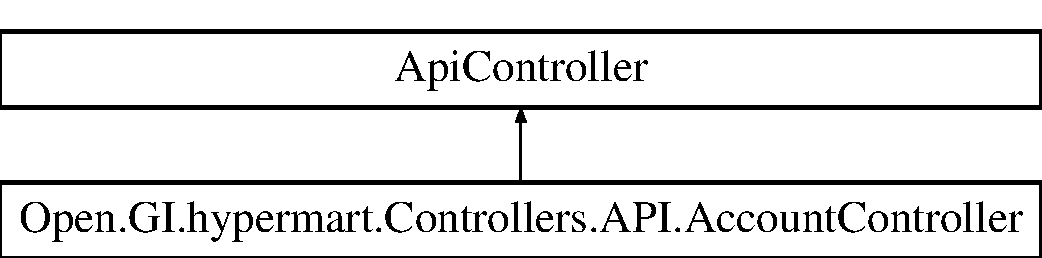
\includegraphics[height=2.000000cm]{class_open_1_1_g_i_1_1hypermart_1_1_controllers_1_1_a_p_i_1_1_account_controller}
\end{center}
\end{figure}
\subsection*{Public Member Functions}
\begin{DoxyCompactItemize}
\item 
\hyperlink{class_open_1_1_g_i_1_1hypermart_1_1_controllers_1_1_a_p_i_1_1_account_controller_ad19bf4f799cb21b28dc2e92454deca5f}{Account\+Controller} ()
\begin{DoxyCompactList}\small\item\em Initializes a new instance of the \hyperlink{class_open_1_1_g_i_1_1hypermart_1_1_controllers_1_1_a_p_i_1_1_account_controller}{Account\+Controller} class. \end{DoxyCompactList}\item 
async Task$<$ I\+Http\+Action\+Result $>$ \hyperlink{class_open_1_1_g_i_1_1hypermart_1_1_controllers_1_1_a_p_i_1_1_account_controller_af7539d8bf4d884854d63a75733ce93e9}{Register} (\hyperlink{class_open_1_1_g_i_1_1hypermart_1_1_models_1_1_user_model}{User\+Model} user\+Model)
\begin{DoxyCompactList}\small\item\em Registers the specified user model. \end{DoxyCompactList}\end{DoxyCompactItemize}
\subsection*{Protected Member Functions}
\begin{DoxyCompactItemize}
\item 
override void \hyperlink{class_open_1_1_g_i_1_1hypermart_1_1_controllers_1_1_a_p_i_1_1_account_controller_a92393dd7d9b1c1d8f2f762ee31fbdd3d}{Dispose} (bool disposing)
\begin{DoxyCompactList}\small\item\em Releases unmanaged and -\/ optionally -\/ managed resources. \end{DoxyCompactList}\end{DoxyCompactItemize}


\subsection{Detailed Description}


\begin{DoxySeeAlso}{See also}
System.\+Web.\+Http.\+Api\+Controller


\end{DoxySeeAlso}


\subsection{Constructor \& Destructor Documentation}
\hypertarget{class_open_1_1_g_i_1_1hypermart_1_1_controllers_1_1_a_p_i_1_1_account_controller_ad19bf4f799cb21b28dc2e92454deca5f}{}\label{class_open_1_1_g_i_1_1hypermart_1_1_controllers_1_1_a_p_i_1_1_account_controller_ad19bf4f799cb21b28dc2e92454deca5f} 
\index{Open\+::\+G\+I\+::hypermart\+::\+Controllers\+::\+A\+P\+I\+::\+Account\+Controller@{Open\+::\+G\+I\+::hypermart\+::\+Controllers\+::\+A\+P\+I\+::\+Account\+Controller}!Account\+Controller@{Account\+Controller}}
\index{Account\+Controller@{Account\+Controller}!Open\+::\+G\+I\+::hypermart\+::\+Controllers\+::\+A\+P\+I\+::\+Account\+Controller@{Open\+::\+G\+I\+::hypermart\+::\+Controllers\+::\+A\+P\+I\+::\+Account\+Controller}}
\subsubsection{\texorpdfstring{Account\+Controller()}{AccountController()}}
{\footnotesize\ttfamily Open.\+G\+I.\+hypermart.\+Controllers.\+A\+P\+I.\+Account\+Controller.\+Account\+Controller (\begin{DoxyParamCaption}{ }\end{DoxyParamCaption})}



Initializes a new instance of the \hyperlink{class_open_1_1_g_i_1_1hypermart_1_1_controllers_1_1_a_p_i_1_1_account_controller}{Account\+Controller} class. 



\subsection{Member Function Documentation}
\hypertarget{class_open_1_1_g_i_1_1hypermart_1_1_controllers_1_1_a_p_i_1_1_account_controller_a92393dd7d9b1c1d8f2f762ee31fbdd3d}{}\label{class_open_1_1_g_i_1_1hypermart_1_1_controllers_1_1_a_p_i_1_1_account_controller_a92393dd7d9b1c1d8f2f762ee31fbdd3d} 
\index{Open\+::\+G\+I\+::hypermart\+::\+Controllers\+::\+A\+P\+I\+::\+Account\+Controller@{Open\+::\+G\+I\+::hypermart\+::\+Controllers\+::\+A\+P\+I\+::\+Account\+Controller}!Dispose@{Dispose}}
\index{Dispose@{Dispose}!Open\+::\+G\+I\+::hypermart\+::\+Controllers\+::\+A\+P\+I\+::\+Account\+Controller@{Open\+::\+G\+I\+::hypermart\+::\+Controllers\+::\+A\+P\+I\+::\+Account\+Controller}}
\subsubsection{\texorpdfstring{Dispose()}{Dispose()}}
{\footnotesize\ttfamily override void Open.\+G\+I.\+hypermart.\+Controllers.\+A\+P\+I.\+Account\+Controller.\+Dispose (\begin{DoxyParamCaption}\item[{bool}]{disposing }\end{DoxyParamCaption})\hspace{0.3cm}{\ttfamily [protected]}}



Releases unmanaged and -\/ optionally -\/ managed resources. 


\begin{DoxyParams}{Parameters}
{\em disposing} & {\ttfamily true} to release both managed and unmanaged resources; {\ttfamily false} to release only unmanaged resources.\\
\hline
\end{DoxyParams}
\hypertarget{class_open_1_1_g_i_1_1hypermart_1_1_controllers_1_1_a_p_i_1_1_account_controller_af7539d8bf4d884854d63a75733ce93e9}{}\label{class_open_1_1_g_i_1_1hypermart_1_1_controllers_1_1_a_p_i_1_1_account_controller_af7539d8bf4d884854d63a75733ce93e9} 
\index{Open\+::\+G\+I\+::hypermart\+::\+Controllers\+::\+A\+P\+I\+::\+Account\+Controller@{Open\+::\+G\+I\+::hypermart\+::\+Controllers\+::\+A\+P\+I\+::\+Account\+Controller}!Register@{Register}}
\index{Register@{Register}!Open\+::\+G\+I\+::hypermart\+::\+Controllers\+::\+A\+P\+I\+::\+Account\+Controller@{Open\+::\+G\+I\+::hypermart\+::\+Controllers\+::\+A\+P\+I\+::\+Account\+Controller}}
\subsubsection{\texorpdfstring{Register()}{Register()}}
{\footnotesize\ttfamily async Task$<$I\+Http\+Action\+Result$>$ Open.\+G\+I.\+hypermart.\+Controllers.\+A\+P\+I.\+Account\+Controller.\+Register (\begin{DoxyParamCaption}\item[{\hyperlink{class_open_1_1_g_i_1_1hypermart_1_1_models_1_1_user_model}{User\+Model}}]{user\+Model }\end{DoxyParamCaption})}



Registers the specified user model. 


\begin{DoxyParams}{Parameters}
{\em user\+Model} & The user model.\\
\hline
\end{DoxyParams}
\begin{DoxyReturn}{Returns}

\end{DoxyReturn}


The documentation for this class was generated from the following file\+:\begin{DoxyCompactItemize}
\item 
C\+:/\+Projects/\+App-\/\+Utility-\/\+Store/\+Open.\+G\+I.\+hypermart/\+Controllers/\+A\+P\+I/\hyperlink{_account_controller_8cs}{Account\+Controller.\+cs}\end{DoxyCompactItemize}

\hypertarget{class_open_1_1_g_i_1_1hypermart_1_1_helpers_1_1_a_d___repository}{}\section{Open.\+G\+I.\+hypermart.\+Helpers.\+A\+D\+\_\+\+Repository Class Reference}
\label{class_open_1_1_g_i_1_1hypermart_1_1_helpers_1_1_a_d___repository}\index{Open.\+G\+I.\+hypermart.\+Helpers.\+A\+D\+\_\+\+Repository@{Open.\+G\+I.\+hypermart.\+Helpers.\+A\+D\+\_\+\+Repository}}


Active Directory Repository  


\subsection*{Public Member Functions}
\begin{DoxyCompactItemize}
\item 
List$<$ \hyperlink{class_open_1_1_g_i_1_1hypermart_1_1_models_1_1_user}{User} $>$ \hyperlink{class_open_1_1_g_i_1_1hypermart_1_1_helpers_1_1_a_d___repository_acf1eb85047c96cf0925f10a7acd96859}{Get\+Users} (string partial\+Name)
\begin{DoxyCompactList}\small\item\em Gets the users. \end{DoxyCompactList}\end{DoxyCompactItemize}
\subsection*{Static Public Member Functions}
\begin{DoxyCompactItemize}
\item 
static Array\+List \hyperlink{class_open_1_1_g_i_1_1hypermart_1_1_helpers_1_1_a_d___repository_a648df6740e7c4c8b603bf8dac1c0d4a1}{Enumerate\+Domains} ()
\begin{DoxyCompactList}\small\item\em Enumerates the domains. \end{DoxyCompactList}\item 
static string \hyperlink{class_open_1_1_g_i_1_1hypermart_1_1_helpers_1_1_a_d___repository_a69769f94231c2d4347184f3b5d6a14a6}{Friendly\+Domain\+To\+Ldap\+Domain} (string friendly\+Domain\+Name)
\begin{DoxyCompactList}\small\item\em Friendlies the domain to L\+D\+AP domain. \end{DoxyCompactList}\item 
static \hyperlink{class_open_1_1_g_i_1_1hypermart_1_1_models_1_1_user}{User} \hyperlink{class_open_1_1_g_i_1_1hypermart_1_1_helpers_1_1_a_d___repository_ab3cdd5f9a962e26fcb50033a5dc4fc0f}{get\+User} (string partial\+Name)
\begin{DoxyCompactList}\small\item\em Gets the user. \end{DoxyCompactList}\end{DoxyCompactItemize}


\subsection{Detailed Description}
Active Directory Repository 



\subsection{Member Function Documentation}
\hypertarget{class_open_1_1_g_i_1_1hypermart_1_1_helpers_1_1_a_d___repository_a648df6740e7c4c8b603bf8dac1c0d4a1}{}\label{class_open_1_1_g_i_1_1hypermart_1_1_helpers_1_1_a_d___repository_a648df6740e7c4c8b603bf8dac1c0d4a1} 
\index{Open\+::\+G\+I\+::hypermart\+::\+Helpers\+::\+A\+D\+\_\+\+Repository@{Open\+::\+G\+I\+::hypermart\+::\+Helpers\+::\+A\+D\+\_\+\+Repository}!Enumerate\+Domains@{Enumerate\+Domains}}
\index{Enumerate\+Domains@{Enumerate\+Domains}!Open\+::\+G\+I\+::hypermart\+::\+Helpers\+::\+A\+D\+\_\+\+Repository@{Open\+::\+G\+I\+::hypermart\+::\+Helpers\+::\+A\+D\+\_\+\+Repository}}
\subsubsection{\texorpdfstring{Enumerate\+Domains()}{EnumerateDomains()}}
{\footnotesize\ttfamily static Array\+List Open.\+G\+I.\+hypermart.\+Helpers.\+A\+D\+\_\+\+Repository.\+Enumerate\+Domains (\begin{DoxyParamCaption}{ }\end{DoxyParamCaption})\hspace{0.3cm}{\ttfamily [static]}}



Enumerates the domains. 

\begin{DoxyReturn}{Returns}

\end{DoxyReturn}
\hypertarget{class_open_1_1_g_i_1_1hypermart_1_1_helpers_1_1_a_d___repository_a69769f94231c2d4347184f3b5d6a14a6}{}\label{class_open_1_1_g_i_1_1hypermart_1_1_helpers_1_1_a_d___repository_a69769f94231c2d4347184f3b5d6a14a6} 
\index{Open\+::\+G\+I\+::hypermart\+::\+Helpers\+::\+A\+D\+\_\+\+Repository@{Open\+::\+G\+I\+::hypermart\+::\+Helpers\+::\+A\+D\+\_\+\+Repository}!Friendly\+Domain\+To\+Ldap\+Domain@{Friendly\+Domain\+To\+Ldap\+Domain}}
\index{Friendly\+Domain\+To\+Ldap\+Domain@{Friendly\+Domain\+To\+Ldap\+Domain}!Open\+::\+G\+I\+::hypermart\+::\+Helpers\+::\+A\+D\+\_\+\+Repository@{Open\+::\+G\+I\+::hypermart\+::\+Helpers\+::\+A\+D\+\_\+\+Repository}}
\subsubsection{\texorpdfstring{Friendly\+Domain\+To\+Ldap\+Domain()}{FriendlyDomainToLdapDomain()}}
{\footnotesize\ttfamily static string Open.\+G\+I.\+hypermart.\+Helpers.\+A\+D\+\_\+\+Repository.\+Friendly\+Domain\+To\+Ldap\+Domain (\begin{DoxyParamCaption}\item[{string}]{friendly\+Domain\+Name }\end{DoxyParamCaption})\hspace{0.3cm}{\ttfamily [static]}}



Friendlies the domain to L\+D\+AP domain. 


\begin{DoxyParams}{Parameters}
{\em friendly\+Domain\+Name} & Name of the friendly domain.\\
\hline
\end{DoxyParams}
\begin{DoxyReturn}{Returns}

\end{DoxyReturn}
\hypertarget{class_open_1_1_g_i_1_1hypermart_1_1_helpers_1_1_a_d___repository_ab3cdd5f9a962e26fcb50033a5dc4fc0f}{}\label{class_open_1_1_g_i_1_1hypermart_1_1_helpers_1_1_a_d___repository_ab3cdd5f9a962e26fcb50033a5dc4fc0f} 
\index{Open\+::\+G\+I\+::hypermart\+::\+Helpers\+::\+A\+D\+\_\+\+Repository@{Open\+::\+G\+I\+::hypermart\+::\+Helpers\+::\+A\+D\+\_\+\+Repository}!get\+User@{get\+User}}
\index{get\+User@{get\+User}!Open\+::\+G\+I\+::hypermart\+::\+Helpers\+::\+A\+D\+\_\+\+Repository@{Open\+::\+G\+I\+::hypermart\+::\+Helpers\+::\+A\+D\+\_\+\+Repository}}
\subsubsection{\texorpdfstring{get\+User()}{getUser()}}
{\footnotesize\ttfamily static \hyperlink{class_open_1_1_g_i_1_1hypermart_1_1_models_1_1_user}{User} Open.\+G\+I.\+hypermart.\+Helpers.\+A\+D\+\_\+\+Repository.\+get\+User (\begin{DoxyParamCaption}\item[{string}]{partial\+Name }\end{DoxyParamCaption})\hspace{0.3cm}{\ttfamily [static]}}



Gets the user. 


\begin{DoxyParams}{Parameters}
{\em partial\+Name} & The partial name.\\
\hline
\end{DoxyParams}
\begin{DoxyReturn}{Returns}
In the event that the user cannot be resolved, then an Empty user will be returned.
\end{DoxyReturn}
\hypertarget{class_open_1_1_g_i_1_1hypermart_1_1_helpers_1_1_a_d___repository_acf1eb85047c96cf0925f10a7acd96859}{}\label{class_open_1_1_g_i_1_1hypermart_1_1_helpers_1_1_a_d___repository_acf1eb85047c96cf0925f10a7acd96859} 
\index{Open\+::\+G\+I\+::hypermart\+::\+Helpers\+::\+A\+D\+\_\+\+Repository@{Open\+::\+G\+I\+::hypermart\+::\+Helpers\+::\+A\+D\+\_\+\+Repository}!Get\+Users@{Get\+Users}}
\index{Get\+Users@{Get\+Users}!Open\+::\+G\+I\+::hypermart\+::\+Helpers\+::\+A\+D\+\_\+\+Repository@{Open\+::\+G\+I\+::hypermart\+::\+Helpers\+::\+A\+D\+\_\+\+Repository}}
\subsubsection{\texorpdfstring{Get\+Users()}{GetUsers()}}
{\footnotesize\ttfamily List$<$\hyperlink{class_open_1_1_g_i_1_1hypermart_1_1_models_1_1_user}{User}$>$ Open.\+G\+I.\+hypermart.\+Helpers.\+A\+D\+\_\+\+Repository.\+Get\+Users (\begin{DoxyParamCaption}\item[{string}]{partial\+Name }\end{DoxyParamCaption})}



Gets the users. 


\begin{DoxyParams}{Parameters}
{\em partial\+Name} & The partial name.\\
\hline
\end{DoxyParams}
\begin{DoxyReturn}{Returns}

\end{DoxyReturn}


The documentation for this class was generated from the following file\+:\begin{DoxyCompactItemize}
\item 
C\+:/\+Projects/\+App-\/\+Utility-\/\+Store/\+Open.\+G\+I.\+hypermart/\+Helpers/\hyperlink{_a_d___repository_8cs}{A\+D\+\_\+\+Repository.\+cs}\end{DoxyCompactItemize}

\hypertarget{class_open_1_1_g_i_1_1hypermart_1_1_attributes_1_1_api_identity}{}\section{Open.\+G\+I.\+hypermart.\+Attributes.\+Api\+Identity Class Reference}
\label{class_open_1_1_g_i_1_1hypermart_1_1_attributes_1_1_api_identity}\index{Open.\+G\+I.\+hypermart.\+Attributes.\+Api\+Identity@{Open.\+G\+I.\+hypermart.\+Attributes.\+Api\+Identity}}


A\+PI identity object  


Inheritance diagram for Open.\+G\+I.\+hypermart.\+Attributes.\+Api\+Identity\+:\begin{figure}[H]
\begin{center}
\leavevmode
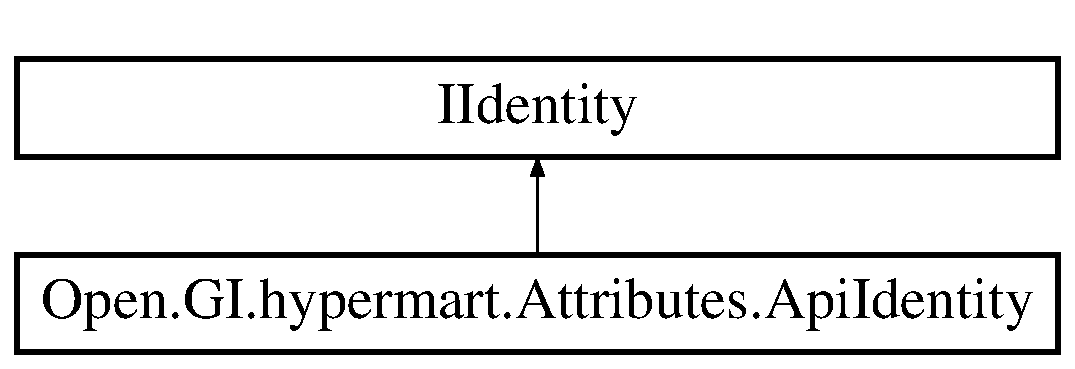
\includegraphics[height=2.000000cm]{class_open_1_1_g_i_1_1hypermart_1_1_attributes_1_1_api_identity}
\end{center}
\end{figure}
\subsection*{Public Member Functions}
\begin{DoxyCompactItemize}
\item 
\hyperlink{class_open_1_1_g_i_1_1hypermart_1_1_attributes_1_1_api_identity_a0ca1c38ef87fde2fb7b816fde06e6ebe}{Api\+Identity} (\hyperlink{class_open_1_1_g_i_1_1hypermart_1_1_models_1_1_w_s_user}{W\+S\+User} user)
\begin{DoxyCompactList}\small\item\em Initializes a new instance of the \hyperlink{class_open_1_1_g_i_1_1hypermart_1_1_attributes_1_1_api_identity}{Api\+Identity} class. \end{DoxyCompactList}\end{DoxyCompactItemize}
\subsection*{Properties}
\begin{DoxyCompactItemize}
\item 
\hyperlink{class_open_1_1_g_i_1_1hypermart_1_1_models_1_1_w_s_user}{W\+S\+User} \hyperlink{class_open_1_1_g_i_1_1hypermart_1_1_attributes_1_1_api_identity_a2335a04152138cb6d766f7553b754204}{User}\hspace{0.3cm}{\ttfamily  \mbox{[}get\mbox{]}}
\begin{DoxyCompactList}\small\item\em Gets the user. \end{DoxyCompactList}\item 
string \hyperlink{class_open_1_1_g_i_1_1hypermart_1_1_attributes_1_1_api_identity_aec1f85ea14352e908d2cbe7e66e27913}{Name}\hspace{0.3cm}{\ttfamily  \mbox{[}get\mbox{]}}
\begin{DoxyCompactList}\small\item\em Gets the name of the current user. \end{DoxyCompactList}\item 
string \hyperlink{class_open_1_1_g_i_1_1hypermart_1_1_attributes_1_1_api_identity_aa3d5a607ebaae15ce9b20556fb633fab}{Authentication\+Type}\hspace{0.3cm}{\ttfamily  \mbox{[}get\mbox{]}}
\begin{DoxyCompactList}\small\item\em Gets the type of authentication used. \end{DoxyCompactList}\item 
bool \hyperlink{class_open_1_1_g_i_1_1hypermart_1_1_attributes_1_1_api_identity_a3407b6da66e2ed782c6f88456b71335f}{Is\+Authenticated}\hspace{0.3cm}{\ttfamily  \mbox{[}get\mbox{]}}
\begin{DoxyCompactList}\small\item\em Gets a value that indicates whether the user has been authenticated. \end{DoxyCompactList}\end{DoxyCompactItemize}


\subsection{Detailed Description}
A\+PI identity object 

\begin{DoxySeeAlso}{See also}
System.\+Security.\+Principal.\+I\+Identity


\end{DoxySeeAlso}


\subsection{Constructor \& Destructor Documentation}
\hypertarget{class_open_1_1_g_i_1_1hypermart_1_1_attributes_1_1_api_identity_a0ca1c38ef87fde2fb7b816fde06e6ebe}{}\label{class_open_1_1_g_i_1_1hypermart_1_1_attributes_1_1_api_identity_a0ca1c38ef87fde2fb7b816fde06e6ebe} 
\index{Open\+::\+G\+I\+::hypermart\+::\+Attributes\+::\+Api\+Identity@{Open\+::\+G\+I\+::hypermart\+::\+Attributes\+::\+Api\+Identity}!Api\+Identity@{Api\+Identity}}
\index{Api\+Identity@{Api\+Identity}!Open\+::\+G\+I\+::hypermart\+::\+Attributes\+::\+Api\+Identity@{Open\+::\+G\+I\+::hypermart\+::\+Attributes\+::\+Api\+Identity}}
\subsubsection{\texorpdfstring{Api\+Identity()}{ApiIdentity()}}
{\footnotesize\ttfamily Open.\+G\+I.\+hypermart.\+Attributes.\+Api\+Identity.\+Api\+Identity (\begin{DoxyParamCaption}\item[{\hyperlink{class_open_1_1_g_i_1_1hypermart_1_1_models_1_1_w_s_user}{W\+S\+User}}]{user }\end{DoxyParamCaption})}



Initializes a new instance of the \hyperlink{class_open_1_1_g_i_1_1hypermart_1_1_attributes_1_1_api_identity}{Api\+Identity} class. 


\begin{DoxyParams}{Parameters}
{\em user} & The user.\\
\hline
\end{DoxyParams}

\begin{DoxyExceptions}{Exceptions}
{\em System.\+Argument\+Null\+Exception} & user\\
\hline
\end{DoxyExceptions}


\subsection{Property Documentation}
\hypertarget{class_open_1_1_g_i_1_1hypermart_1_1_attributes_1_1_api_identity_aa3d5a607ebaae15ce9b20556fb633fab}{}\label{class_open_1_1_g_i_1_1hypermart_1_1_attributes_1_1_api_identity_aa3d5a607ebaae15ce9b20556fb633fab} 
\index{Open\+::\+G\+I\+::hypermart\+::\+Attributes\+::\+Api\+Identity@{Open\+::\+G\+I\+::hypermart\+::\+Attributes\+::\+Api\+Identity}!Authentication\+Type@{Authentication\+Type}}
\index{Authentication\+Type@{Authentication\+Type}!Open\+::\+G\+I\+::hypermart\+::\+Attributes\+::\+Api\+Identity@{Open\+::\+G\+I\+::hypermart\+::\+Attributes\+::\+Api\+Identity}}
\subsubsection{\texorpdfstring{Authentication\+Type}{AuthenticationType}}
{\footnotesize\ttfamily string Open.\+G\+I.\+hypermart.\+Attributes.\+Api\+Identity.\+Authentication\+Type\hspace{0.3cm}{\ttfamily [get]}}



Gets the type of authentication used. 

\hypertarget{class_open_1_1_g_i_1_1hypermart_1_1_attributes_1_1_api_identity_a3407b6da66e2ed782c6f88456b71335f}{}\label{class_open_1_1_g_i_1_1hypermart_1_1_attributes_1_1_api_identity_a3407b6da66e2ed782c6f88456b71335f} 
\index{Open\+::\+G\+I\+::hypermart\+::\+Attributes\+::\+Api\+Identity@{Open\+::\+G\+I\+::hypermart\+::\+Attributes\+::\+Api\+Identity}!Is\+Authenticated@{Is\+Authenticated}}
\index{Is\+Authenticated@{Is\+Authenticated}!Open\+::\+G\+I\+::hypermart\+::\+Attributes\+::\+Api\+Identity@{Open\+::\+G\+I\+::hypermart\+::\+Attributes\+::\+Api\+Identity}}
\subsubsection{\texorpdfstring{Is\+Authenticated}{IsAuthenticated}}
{\footnotesize\ttfamily bool Open.\+G\+I.\+hypermart.\+Attributes.\+Api\+Identity.\+Is\+Authenticated\hspace{0.3cm}{\ttfamily [get]}}



Gets a value that indicates whether the user has been authenticated. 

\hypertarget{class_open_1_1_g_i_1_1hypermart_1_1_attributes_1_1_api_identity_aec1f85ea14352e908d2cbe7e66e27913}{}\label{class_open_1_1_g_i_1_1hypermart_1_1_attributes_1_1_api_identity_aec1f85ea14352e908d2cbe7e66e27913} 
\index{Open\+::\+G\+I\+::hypermart\+::\+Attributes\+::\+Api\+Identity@{Open\+::\+G\+I\+::hypermart\+::\+Attributes\+::\+Api\+Identity}!Name@{Name}}
\index{Name@{Name}!Open\+::\+G\+I\+::hypermart\+::\+Attributes\+::\+Api\+Identity@{Open\+::\+G\+I\+::hypermart\+::\+Attributes\+::\+Api\+Identity}}
\subsubsection{\texorpdfstring{Name}{Name}}
{\footnotesize\ttfamily string Open.\+G\+I.\+hypermart.\+Attributes.\+Api\+Identity.\+Name\hspace{0.3cm}{\ttfamily [get]}}



Gets the name of the current user. 

\hypertarget{class_open_1_1_g_i_1_1hypermart_1_1_attributes_1_1_api_identity_a2335a04152138cb6d766f7553b754204}{}\label{class_open_1_1_g_i_1_1hypermart_1_1_attributes_1_1_api_identity_a2335a04152138cb6d766f7553b754204} 
\index{Open\+::\+G\+I\+::hypermart\+::\+Attributes\+::\+Api\+Identity@{Open\+::\+G\+I\+::hypermart\+::\+Attributes\+::\+Api\+Identity}!User@{User}}
\index{User@{User}!Open\+::\+G\+I\+::hypermart\+::\+Attributes\+::\+Api\+Identity@{Open\+::\+G\+I\+::hypermart\+::\+Attributes\+::\+Api\+Identity}}
\subsubsection{\texorpdfstring{User}{User}}
{\footnotesize\ttfamily \hyperlink{class_open_1_1_g_i_1_1hypermart_1_1_models_1_1_w_s_user}{W\+S\+User} Open.\+G\+I.\+hypermart.\+Attributes.\+Api\+Identity.\+User\hspace{0.3cm}{\ttfamily [get]}}



Gets the user. 

The user. 

The documentation for this class was generated from the following file\+:\begin{DoxyCompactItemize}
\item 
C\+:/\+Projects/\+App-\/\+Utility-\/\+Store/\+Open.\+G\+I.\+hypermart/\+Attributes/\hyperlink{_api_identity_8cs}{Api\+Identity.\+cs}\end{DoxyCompactItemize}

\hypertarget{class_open_1_1_g_i_1_1hypermart_1_1_helpers_1_1_atom_action_result}{}\section{Open.\+G\+I.\+hypermart.\+Helpers.\+Atom\+Action\+Result Class Reference}
\label{class_open_1_1_g_i_1_1hypermart_1_1_helpers_1_1_atom_action_result}\index{Open.\+G\+I.\+hypermart.\+Helpers.\+Atom\+Action\+Result@{Open.\+G\+I.\+hypermart.\+Helpers.\+Atom\+Action\+Result}}


Creates an A\+T\+O\+M Result  


Inheritance diagram for Open.\+G\+I.\+hypermart.\+Helpers.\+Atom\+Action\+Result\+:\begin{figure}[H]
\begin{center}
\leavevmode
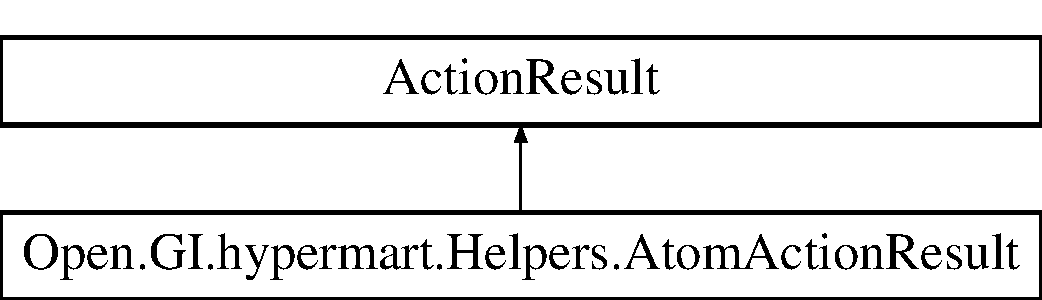
\includegraphics[height=2.000000cm]{class_open_1_1_g_i_1_1hypermart_1_1_helpers_1_1_atom_action_result}
\end{center}
\end{figure}
\subsection*{Public Member Functions}
\begin{DoxyCompactItemize}
\item 
override void \hyperlink{class_open_1_1_g_i_1_1hypermart_1_1_helpers_1_1_atom_action_result_a525b622f00e4c2294a4fedb438273981}{Execute\+Result} (Controller\+Context context)
\begin{DoxyCompactList}\small\item\em Enables processing of the result of an action method by a custom type that inherits from the T\+:\+System.\+Web.\+Mvc.\+Action\+Result class. \end{DoxyCompactList}\end{DoxyCompactItemize}
\subsection*{Properties}
\begin{DoxyCompactItemize}
\item 
Syndication\+Feed \hyperlink{class_open_1_1_g_i_1_1hypermart_1_1_helpers_1_1_atom_action_result_a17a5a951bdf5ed9f8a93f24843e124ca}{Feed}\hspace{0.3cm}{\ttfamily  \mbox{[}get, set\mbox{]}}
\begin{DoxyCompactList}\small\item\em Gets or sets the feed. \end{DoxyCompactList}\end{DoxyCompactItemize}


\subsection{Detailed Description}
Creates an A\+T\+O\+M Result 

\begin{DoxySeeAlso}{See also}
System.\+Web.\+Mvc.\+Action\+Result


\end{DoxySeeAlso}


Definition at line 14 of file Rss\+Action\+Result.\+cs.



\subsection{Member Function Documentation}
\hypertarget{class_open_1_1_g_i_1_1hypermart_1_1_helpers_1_1_atom_action_result_a525b622f00e4c2294a4fedb438273981}{}\index{Open\+::\+G\+I\+::hypermart\+::\+Helpers\+::\+Atom\+Action\+Result@{Open\+::\+G\+I\+::hypermart\+::\+Helpers\+::\+Atom\+Action\+Result}!Execute\+Result@{Execute\+Result}}
\index{Execute\+Result@{Execute\+Result}!Open\+::\+G\+I\+::hypermart\+::\+Helpers\+::\+Atom\+Action\+Result@{Open\+::\+G\+I\+::hypermart\+::\+Helpers\+::\+Atom\+Action\+Result}}
\subsubsection[{Execute\+Result(\+Controller\+Context context)}]{\setlength{\rightskip}{0pt plus 5cm}override void Open.\+G\+I.\+hypermart.\+Helpers.\+Atom\+Action\+Result.\+Execute\+Result (
\begin{DoxyParamCaption}
\item[{Controller\+Context}]{context}
\end{DoxyParamCaption}
)}\label{class_open_1_1_g_i_1_1hypermart_1_1_helpers_1_1_atom_action_result_a525b622f00e4c2294a4fedb438273981}


Enables processing of the result of an action method by a custom type that inherits from the T\+:\+System.\+Web.\+Mvc.\+Action\+Result class. 


\begin{DoxyParams}{Parameters}
{\em context} & The context in which the result is executed. The context information includes the controller, H\+T\+T\+P content, request context, and route data.\\
\hline
\end{DoxyParams}


Definition at line 28 of file Rss\+Action\+Result.\+cs.



\subsection{Property Documentation}
\hypertarget{class_open_1_1_g_i_1_1hypermart_1_1_helpers_1_1_atom_action_result_a17a5a951bdf5ed9f8a93f24843e124ca}{}\index{Open\+::\+G\+I\+::hypermart\+::\+Helpers\+::\+Atom\+Action\+Result@{Open\+::\+G\+I\+::hypermart\+::\+Helpers\+::\+Atom\+Action\+Result}!Feed@{Feed}}
\index{Feed@{Feed}!Open\+::\+G\+I\+::hypermart\+::\+Helpers\+::\+Atom\+Action\+Result@{Open\+::\+G\+I\+::hypermart\+::\+Helpers\+::\+Atom\+Action\+Result}}
\subsubsection[{Feed}]{\setlength{\rightskip}{0pt plus 5cm}Syndication\+Feed Open.\+G\+I.\+hypermart.\+Helpers.\+Atom\+Action\+Result.\+Feed\hspace{0.3cm}{\ttfamily [get]}, {\ttfamily [set]}}\label{class_open_1_1_g_i_1_1hypermart_1_1_helpers_1_1_atom_action_result_a17a5a951bdf5ed9f8a93f24843e124ca}


Gets or sets the feed. 

The feed. 

Definition at line 22 of file Rss\+Action\+Result.\+cs.



The documentation for this class was generated from the following file\+:\begin{DoxyCompactItemize}
\item 
C\+:/\+Projects/\+App-\/\+Utility-\/\+Store/\+Open.\+G\+I.\+hypermart/\+Helpers/\hyperlink{_rss_action_result_8cs}{Rss\+Action\+Result.\+cs}\end{DoxyCompactItemize}

\section{Open.\+G\+I.\+hypermart.\+D\+A\+L.\+Auth\+Context Class Reference}
\label{class_open_1_1_g_i_1_1hypermart_1_1_d_a_l_1_1_auth_context}\index{Open.\+G\+I.\+hypermart.\+D\+A\+L.\+Auth\+Context@{Open.\+G\+I.\+hypermart.\+D\+A\+L.\+Auth\+Context}}


 


Inheritance diagram for Open.\+G\+I.\+hypermart.\+D\+A\+L.\+Auth\+Context\+:\begin{figure}[H]
\begin{center}
\leavevmode
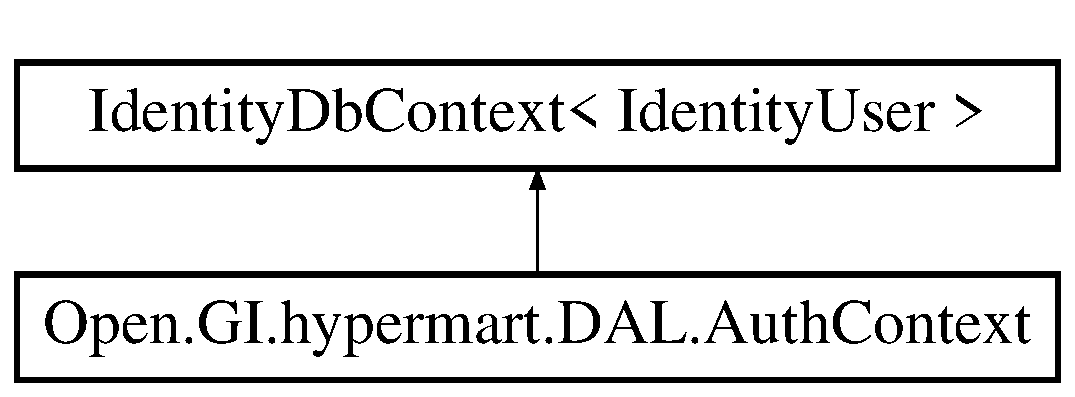
\includegraphics[height=2.000000cm]{class_open_1_1_g_i_1_1hypermart_1_1_d_a_l_1_1_auth_context}
\end{center}
\end{figure}
\subsection*{Public Member Functions}
\begin{DoxyCompactItemize}
\item 
\textbf{ Auth\+Context} ()
\begin{DoxyCompactList}\small\item\em Initializes a new instance of the \doxyref{Auth\+Context}{p.}{class_open_1_1_g_i_1_1hypermart_1_1_d_a_l_1_1_auth_context} class. \end{DoxyCompactList}\end{DoxyCompactItemize}


\subsection{Detailed Description}




Definition at line 14 of file Auth\+Context.\+cs.



\subsection{Constructor \& Destructor Documentation}
\mbox{\label{class_open_1_1_g_i_1_1hypermart_1_1_d_a_l_1_1_auth_context_ad497de9f8875b2f08c83fea4f5086dd1}} 
\index{Open\+::\+G\+I\+::hypermart\+::\+D\+A\+L\+::\+Auth\+Context@{Open\+::\+G\+I\+::hypermart\+::\+D\+A\+L\+::\+Auth\+Context}!Auth\+Context@{Auth\+Context}}
\index{Auth\+Context@{Auth\+Context}!Open\+::\+G\+I\+::hypermart\+::\+D\+A\+L\+::\+Auth\+Context@{Open\+::\+G\+I\+::hypermart\+::\+D\+A\+L\+::\+Auth\+Context}}
\subsubsection{Auth\+Context()}
{\footnotesize\ttfamily Open.\+G\+I.\+hypermart.\+D\+A\+L.\+Auth\+Context.\+Auth\+Context (\begin{DoxyParamCaption}{ }\end{DoxyParamCaption})}



Initializes a new instance of the \doxyref{Auth\+Context}{p.}{class_open_1_1_g_i_1_1hypermart_1_1_d_a_l_1_1_auth_context} class. 



Definition at line 19 of file Auth\+Context.\+cs.



The documentation for this class was generated from the following file\+:\begin{DoxyCompactItemize}
\item 
C\+:/\+Projects/\+App-\/\+Utility-\/\+Store/\+Open.\+G\+I.\+hypermart/\+D\+A\+L/\textbf{ Auth\+Context.\+cs}\end{DoxyCompactItemize}

\section{Open.\+G\+I.\+hypermart.\+Helpers.\+Auth\+Repository Class Reference}
\label{class_open_1_1_g_i_1_1hypermart_1_1_helpers_1_1_auth_repository}\index{Open.\+G\+I.\+hypermart.\+Helpers.\+Auth\+Repository@{Open.\+G\+I.\+hypermart.\+Helpers.\+Auth\+Repository}}


 


Inheritance diagram for Open.\+G\+I.\+hypermart.\+Helpers.\+Auth\+Repository\+:\begin{figure}[H]
\begin{center}
\leavevmode
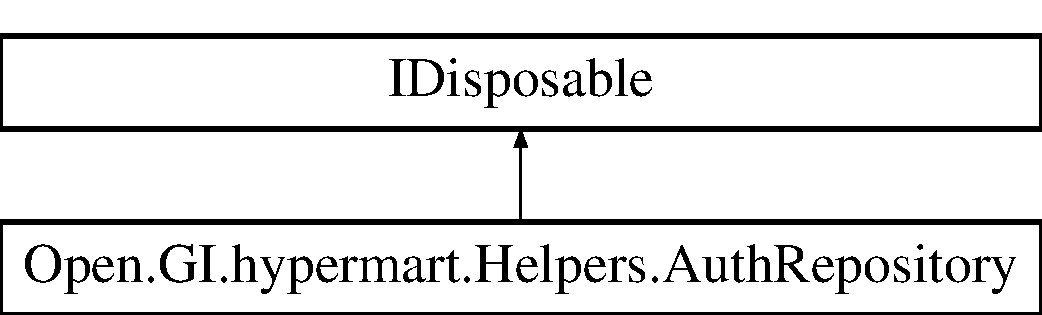
\includegraphics[height=2.000000cm]{class_open_1_1_g_i_1_1hypermart_1_1_helpers_1_1_auth_repository}
\end{center}
\end{figure}
\subsection*{Public Member Functions}
\begin{DoxyCompactItemize}
\item 
\textbf{ Auth\+Repository} ()
\begin{DoxyCompactList}\small\item\em Initializes a new instance of the \doxyref{Auth\+Repository}{p.}{class_open_1_1_g_i_1_1hypermart_1_1_helpers_1_1_auth_repository} class. \end{DoxyCompactList}\item 
async Task$<$ Identity\+Result $>$ \textbf{ Register\+User} (\textbf{ User\+Model} user\+Model)
\begin{DoxyCompactList}\small\item\em Registers the user. \end{DoxyCompactList}\item 
async Task$<$ Identity\+User $>$ \textbf{ Find\+User} (string user\+Name, string password)
\begin{DoxyCompactList}\small\item\em Finds the user. \end{DoxyCompactList}\item 
void \textbf{ Dispose} ()
\begin{DoxyCompactList}\small\item\em Performs application-\/defined tasks associated with freeing, releasing, or resetting unmanaged resources. \end{DoxyCompactList}\end{DoxyCompactItemize}


\subsection{Detailed Description}


\begin{DoxySeeAlso}{See also}
System.\+I\+Disposable


\end{DoxySeeAlso}


Definition at line 17 of file Auth\+Repository.\+cs.



\subsection{Constructor \& Destructor Documentation}
\mbox{\label{class_open_1_1_g_i_1_1hypermart_1_1_helpers_1_1_auth_repository_a45b19c0a6f979f86ae43cbded49aeb5a}} 
\index{Open\+::\+G\+I\+::hypermart\+::\+Helpers\+::\+Auth\+Repository@{Open\+::\+G\+I\+::hypermart\+::\+Helpers\+::\+Auth\+Repository}!Auth\+Repository@{Auth\+Repository}}
\index{Auth\+Repository@{Auth\+Repository}!Open\+::\+G\+I\+::hypermart\+::\+Helpers\+::\+Auth\+Repository@{Open\+::\+G\+I\+::hypermart\+::\+Helpers\+::\+Auth\+Repository}}
\subsubsection{Auth\+Repository()}
{\footnotesize\ttfamily Open.\+G\+I.\+hypermart.\+Helpers.\+Auth\+Repository.\+Auth\+Repository (\begin{DoxyParamCaption}{ }\end{DoxyParamCaption})}



Initializes a new instance of the \doxyref{Auth\+Repository}{p.}{class_open_1_1_g_i_1_1hypermart_1_1_helpers_1_1_auth_repository} class. 



Definition at line 25 of file Auth\+Repository.\+cs.



\subsection{Member Function Documentation}
\mbox{\label{class_open_1_1_g_i_1_1hypermart_1_1_helpers_1_1_auth_repository_afd0cd6f5615edaecc5395a7d60c769a6}} 
\index{Open\+::\+G\+I\+::hypermart\+::\+Helpers\+::\+Auth\+Repository@{Open\+::\+G\+I\+::hypermart\+::\+Helpers\+::\+Auth\+Repository}!Dispose@{Dispose}}
\index{Dispose@{Dispose}!Open\+::\+G\+I\+::hypermart\+::\+Helpers\+::\+Auth\+Repository@{Open\+::\+G\+I\+::hypermart\+::\+Helpers\+::\+Auth\+Repository}}
\subsubsection{Dispose()}
{\footnotesize\ttfamily void Open.\+G\+I.\+hypermart.\+Helpers.\+Auth\+Repository.\+Dispose (\begin{DoxyParamCaption}{ }\end{DoxyParamCaption})}



Performs application-\/defined tasks associated with freeing, releasing, or resetting unmanaged resources. 



Definition at line 61 of file Auth\+Repository.\+cs.

\mbox{\label{class_open_1_1_g_i_1_1hypermart_1_1_helpers_1_1_auth_repository_afe19f379cb79c18b95ae18be218960a6}} 
\index{Open\+::\+G\+I\+::hypermart\+::\+Helpers\+::\+Auth\+Repository@{Open\+::\+G\+I\+::hypermart\+::\+Helpers\+::\+Auth\+Repository}!Find\+User@{Find\+User}}
\index{Find\+User@{Find\+User}!Open\+::\+G\+I\+::hypermart\+::\+Helpers\+::\+Auth\+Repository@{Open\+::\+G\+I\+::hypermart\+::\+Helpers\+::\+Auth\+Repository}}
\subsubsection{Find\+User()}
{\footnotesize\ttfamily async Task$<$Identity\+User$>$ Open.\+G\+I.\+hypermart.\+Helpers.\+Auth\+Repository.\+Find\+User (\begin{DoxyParamCaption}\item[{string}]{user\+Name,  }\item[{string}]{password }\end{DoxyParamCaption})}



Finds the user. 


\begin{DoxyParams}{Parameters}
{\em user\+Name} & Name of the user.\\
\hline
{\em password} & The password.\\
\hline
\end{DoxyParams}
\begin{DoxyReturn}{Returns}

\end{DoxyReturn}


Definition at line 52 of file Auth\+Repository.\+cs.

\mbox{\label{class_open_1_1_g_i_1_1hypermart_1_1_helpers_1_1_auth_repository_aedc26a57af08ecb4a9cae4ab46055bf9}} 
\index{Open\+::\+G\+I\+::hypermart\+::\+Helpers\+::\+Auth\+Repository@{Open\+::\+G\+I\+::hypermart\+::\+Helpers\+::\+Auth\+Repository}!Register\+User@{Register\+User}}
\index{Register\+User@{Register\+User}!Open\+::\+G\+I\+::hypermart\+::\+Helpers\+::\+Auth\+Repository@{Open\+::\+G\+I\+::hypermart\+::\+Helpers\+::\+Auth\+Repository}}
\subsubsection{Register\+User()}
{\footnotesize\ttfamily async Task$<$Identity\+Result$>$ Open.\+G\+I.\+hypermart.\+Helpers.\+Auth\+Repository.\+Register\+User (\begin{DoxyParamCaption}\item[{\textbf{ User\+Model}}]{user\+Model }\end{DoxyParamCaption})}



Registers the user. 


\begin{DoxyParams}{Parameters}
{\em user\+Model} & The user model.\\
\hline
\end{DoxyParams}
\begin{DoxyReturn}{Returns}

\end{DoxyReturn}


Definition at line 35 of file Auth\+Repository.\+cs.



The documentation for this class was generated from the following file\+:\begin{DoxyCompactItemize}
\item 
C\+:/\+Projects/\+App-\/\+Utility-\/\+Store/\+Open.\+G\+I.\+hypermart/\+Helpers/\textbf{ Auth\+Repository.\+cs}\end{DoxyCompactItemize}

\hypertarget{class_open_1_1_g_i_1_1hypermart_1_1_bundle_config}{}\section{Open.\+G\+I.\+hypermart.\+Bundle\+Config Class Reference}
\label{class_open_1_1_g_i_1_1hypermart_1_1_bundle_config}\index{Open.\+G\+I.\+hypermart.\+Bundle\+Config@{Open.\+G\+I.\+hypermart.\+Bundle\+Config}}


A\+S\+P.\+N\+ET M\+VC Bundle configuration  


\subsection*{Static Public Member Functions}
\begin{DoxyCompactItemize}
\item 
static void \hyperlink{class_open_1_1_g_i_1_1hypermart_1_1_bundle_config_a7b372315a10361265239dc75c616207e}{Register\+Bundles} (Bundle\+Collection bundles)
\begin{DoxyCompactList}\small\item\em Registers the bundles. \end{DoxyCompactList}\end{DoxyCompactItemize}


\subsection{Detailed Description}
A\+S\+P.\+N\+ET M\+VC Bundle configuration 



\subsection{Member Function Documentation}
\hypertarget{class_open_1_1_g_i_1_1hypermart_1_1_bundle_config_a7b372315a10361265239dc75c616207e}{}\label{class_open_1_1_g_i_1_1hypermart_1_1_bundle_config_a7b372315a10361265239dc75c616207e} 
\index{Open\+::\+G\+I\+::hypermart\+::\+Bundle\+Config@{Open\+::\+G\+I\+::hypermart\+::\+Bundle\+Config}!Register\+Bundles@{Register\+Bundles}}
\index{Register\+Bundles@{Register\+Bundles}!Open\+::\+G\+I\+::hypermart\+::\+Bundle\+Config@{Open\+::\+G\+I\+::hypermart\+::\+Bundle\+Config}}
\subsubsection{\texorpdfstring{Register\+Bundles()}{RegisterBundles()}}
{\footnotesize\ttfamily static void Open.\+G\+I.\+hypermart.\+Bundle\+Config.\+Register\+Bundles (\begin{DoxyParamCaption}\item[{Bundle\+Collection}]{bundles }\end{DoxyParamCaption})\hspace{0.3cm}{\ttfamily [static]}}



Registers the bundles. 


\begin{DoxyParams}{Parameters}
{\em bundles} & The bundles.\\
\hline
\end{DoxyParams}


The documentation for this class was generated from the following file\+:\begin{DoxyCompactItemize}
\item 
C\+:/\+Projects/\+App-\/\+Utility-\/\+Store/\+Open.\+G\+I.\+hypermart/\+App\+\_\+\+Start/\hyperlink{_bundle_config_8cs}{Bundle\+Config.\+cs}\end{DoxyCompactItemize}

\hypertarget{class_open_1_1_g_i_1_1hypermart_1_1_models_1_1_category}{}\section{Open.\+G\+I.\+hypermart.\+Models.\+Category Class Reference}
\label{class_open_1_1_g_i_1_1hypermart_1_1_models_1_1_category}\index{Open.\+G\+I.\+hypermart.\+Models.\+Category@{Open.\+G\+I.\+hypermart.\+Models.\+Category}}


 




\subsection{Detailed Description}




The documentation for this class was generated from the following file\+:\begin{DoxyCompactItemize}
\item 
C\+:/\+Projects/\+App-\/\+Utility-\/\+Store/\+Open.\+G\+I.\+hypermart/\+Models/\hyperlink{_category_8cs}{Category.\+cs}\end{DoxyCompactItemize}

\hypertarget{class_open_1_1_g_i_1_1hypermart_1_1_areas_1_1_help_page_1_1_model_descriptions_1_1_collection_model_description}{}\section{Open.\+G\+I.\+hypermart.\+Areas.\+Help\+Page.\+Model\+Descriptions.\+Collection\+Model\+Description Class Reference}
\label{class_open_1_1_g_i_1_1hypermart_1_1_areas_1_1_help_page_1_1_model_descriptions_1_1_collection_model_description}\index{Open.\+G\+I.\+hypermart.\+Areas.\+Help\+Page.\+Model\+Descriptions.\+Collection\+Model\+Description@{Open.\+G\+I.\+hypermart.\+Areas.\+Help\+Page.\+Model\+Descriptions.\+Collection\+Model\+Description}}


 


Inheritance diagram for Open.\+G\+I.\+hypermart.\+Areas.\+Help\+Page.\+Model\+Descriptions.\+Collection\+Model\+Description\+:\begin{figure}[H]
\begin{center}
\leavevmode
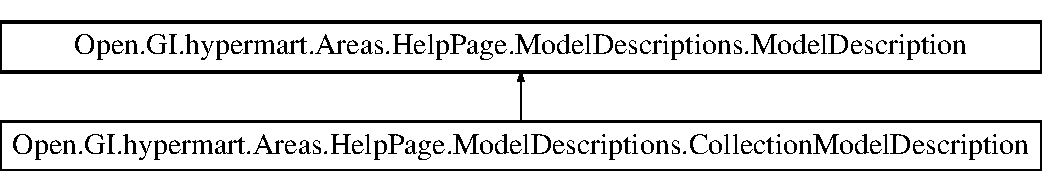
\includegraphics[height=2.000000cm]{class_open_1_1_g_i_1_1hypermart_1_1_areas_1_1_help_page_1_1_model_descriptions_1_1_collection_model_description}
\end{center}
\end{figure}
\subsection*{Properties}
\begin{DoxyCompactItemize}
\item 
\hyperlink{class_open_1_1_g_i_1_1hypermart_1_1_areas_1_1_help_page_1_1_model_descriptions_1_1_model_description}{Model\+Description} \hyperlink{class_open_1_1_g_i_1_1hypermart_1_1_areas_1_1_help_page_1_1_model_descriptions_1_1_collection_model_description_a4049e2a56d1af746b241c4ae2da109ca}{Element\+Description}\hspace{0.3cm}{\ttfamily  \mbox{[}get, set\mbox{]}}
\begin{DoxyCompactList}\small\item\em Gets or sets the element description. \end{DoxyCompactList}\end{DoxyCompactItemize}


\subsection{Detailed Description}


\begin{DoxySeeAlso}{See also}
\hyperlink{class_open_1_1_g_i_1_1hypermart_1_1_areas_1_1_help_page_1_1_model_descriptions_1_1_model_description}{Open.\+G\+I.\+hypermart.\+Areas.\+Help\+Page.\+Model\+Descriptions.\+Model\+Description}


\end{DoxySeeAlso}


\subsection{Property Documentation}
\hypertarget{class_open_1_1_g_i_1_1hypermart_1_1_areas_1_1_help_page_1_1_model_descriptions_1_1_collection_model_description_a4049e2a56d1af746b241c4ae2da109ca}{}\label{class_open_1_1_g_i_1_1hypermart_1_1_areas_1_1_help_page_1_1_model_descriptions_1_1_collection_model_description_a4049e2a56d1af746b241c4ae2da109ca} 
\index{Open\+::\+G\+I\+::hypermart\+::\+Areas\+::\+Help\+Page\+::\+Model\+Descriptions\+::\+Collection\+Model\+Description@{Open\+::\+G\+I\+::hypermart\+::\+Areas\+::\+Help\+Page\+::\+Model\+Descriptions\+::\+Collection\+Model\+Description}!Element\+Description@{Element\+Description}}
\index{Element\+Description@{Element\+Description}!Open\+::\+G\+I\+::hypermart\+::\+Areas\+::\+Help\+Page\+::\+Model\+Descriptions\+::\+Collection\+Model\+Description@{Open\+::\+G\+I\+::hypermart\+::\+Areas\+::\+Help\+Page\+::\+Model\+Descriptions\+::\+Collection\+Model\+Description}}
\subsubsection{\texorpdfstring{Element\+Description}{ElementDescription}}
{\footnotesize\ttfamily \hyperlink{class_open_1_1_g_i_1_1hypermart_1_1_areas_1_1_help_page_1_1_model_descriptions_1_1_model_description}{Model\+Description} Open.\+G\+I.\+hypermart.\+Areas.\+Help\+Page.\+Model\+Descriptions.\+Collection\+Model\+Description.\+Element\+Description\hspace{0.3cm}{\ttfamily [get]}, {\ttfamily [set]}}



Gets or sets the element description. 

The element description. 

The documentation for this class was generated from the following file\+:\begin{DoxyCompactItemize}
\item 
C\+:/\+Projects/\+App-\/\+Utility-\/\+Store/\+Open.\+G\+I.\+hypermart/\+Areas/\+Help\+Page/\+Model\+Descriptions/\hyperlink{_collection_model_description_8cs}{Collection\+Model\+Description.\+cs}\end{DoxyCompactItemize}

\section{Open.\+G\+I.\+hypermart.\+Areas.\+Help\+Page.\+Model\+Descriptions.\+Complex\+Type\+Model\+Description Class Reference}
\label{class_open_1_1_g_i_1_1hypermart_1_1_areas_1_1_help_page_1_1_model_descriptions_1_1_complex_type_model_description}\index{Open.\+G\+I.\+hypermart.\+Areas.\+Help\+Page.\+Model\+Descriptions.\+Complex\+Type\+Model\+Description@{Open.\+G\+I.\+hypermart.\+Areas.\+Help\+Page.\+Model\+Descriptions.\+Complex\+Type\+Model\+Description}}


 


Inheritance diagram for Open.\+G\+I.\+hypermart.\+Areas.\+Help\+Page.\+Model\+Descriptions.\+Complex\+Type\+Model\+Description\+:\begin{figure}[H]
\begin{center}
\leavevmode
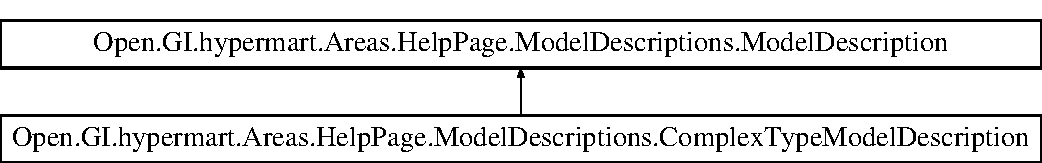
\includegraphics[height=2.000000cm]{class_open_1_1_g_i_1_1hypermart_1_1_areas_1_1_help_page_1_1_model_descriptions_1_1_complex_type_model_description}
\end{center}
\end{figure}
\subsection*{Public Member Functions}
\begin{DoxyCompactItemize}
\item 
\textbf{ Complex\+Type\+Model\+Description} ()
\begin{DoxyCompactList}\small\item\em Initializes a new instance of the \doxyref{Complex\+Type\+Model\+Description}{p.}{class_open_1_1_g_i_1_1hypermart_1_1_areas_1_1_help_page_1_1_model_descriptions_1_1_complex_type_model_description} class. \end{DoxyCompactList}\end{DoxyCompactItemize}
\subsection*{Properties}
\begin{DoxyCompactItemize}
\item 
Collection$<$ \textbf{ Parameter\+Description} $>$ \textbf{ Properties}\hspace{0.3cm}{\ttfamily  [get]}
\begin{DoxyCompactList}\small\item\em Gets the properties. \end{DoxyCompactList}\end{DoxyCompactItemize}


\subsection{Detailed Description}


\begin{DoxySeeAlso}{See also}
\doxyref{Open.\+G\+I.\+hypermart.\+Areas.\+Help\+Page.\+Model\+Descriptions.\+Model\+Description}{p.}{class_open_1_1_g_i_1_1hypermart_1_1_areas_1_1_help_page_1_1_model_descriptions_1_1_model_description}


\end{DoxySeeAlso}


Definition at line 9 of file Complex\+Type\+Model\+Description.\+cs.



\subsection{Constructor \& Destructor Documentation}
\mbox{\label{class_open_1_1_g_i_1_1hypermart_1_1_areas_1_1_help_page_1_1_model_descriptions_1_1_complex_type_model_description_a750b8a599e8e45d091aebfb26edfb3cd}} 
\index{Open\+::\+G\+I\+::hypermart\+::\+Areas\+::\+Help\+Page\+::\+Model\+Descriptions\+::\+Complex\+Type\+Model\+Description@{Open\+::\+G\+I\+::hypermart\+::\+Areas\+::\+Help\+Page\+::\+Model\+Descriptions\+::\+Complex\+Type\+Model\+Description}!Complex\+Type\+Model\+Description@{Complex\+Type\+Model\+Description}}
\index{Complex\+Type\+Model\+Description@{Complex\+Type\+Model\+Description}!Open\+::\+G\+I\+::hypermart\+::\+Areas\+::\+Help\+Page\+::\+Model\+Descriptions\+::\+Complex\+Type\+Model\+Description@{Open\+::\+G\+I\+::hypermart\+::\+Areas\+::\+Help\+Page\+::\+Model\+Descriptions\+::\+Complex\+Type\+Model\+Description}}
\subsubsection{Complex\+Type\+Model\+Description()}
{\footnotesize\ttfamily Open.\+G\+I.\+hypermart.\+Areas.\+Help\+Page.\+Model\+Descriptions.\+Complex\+Type\+Model\+Description.\+Complex\+Type\+Model\+Description (\begin{DoxyParamCaption}{ }\end{DoxyParamCaption})}



Initializes a new instance of the \doxyref{Complex\+Type\+Model\+Description}{p.}{class_open_1_1_g_i_1_1hypermart_1_1_areas_1_1_help_page_1_1_model_descriptions_1_1_complex_type_model_description} class. 



Definition at line 14 of file Complex\+Type\+Model\+Description.\+cs.



\subsection{Property Documentation}
\mbox{\label{class_open_1_1_g_i_1_1hypermart_1_1_areas_1_1_help_page_1_1_model_descriptions_1_1_complex_type_model_description_aef12ede0391a6d743c2f92b1f94d46c2}} 
\index{Open\+::\+G\+I\+::hypermart\+::\+Areas\+::\+Help\+Page\+::\+Model\+Descriptions\+::\+Complex\+Type\+Model\+Description@{Open\+::\+G\+I\+::hypermart\+::\+Areas\+::\+Help\+Page\+::\+Model\+Descriptions\+::\+Complex\+Type\+Model\+Description}!Properties@{Properties}}
\index{Properties@{Properties}!Open\+::\+G\+I\+::hypermart\+::\+Areas\+::\+Help\+Page\+::\+Model\+Descriptions\+::\+Complex\+Type\+Model\+Description@{Open\+::\+G\+I\+::hypermart\+::\+Areas\+::\+Help\+Page\+::\+Model\+Descriptions\+::\+Complex\+Type\+Model\+Description}}
\subsubsection{Properties}
{\footnotesize\ttfamily Collection$<$\textbf{ Parameter\+Description}$>$ Open.\+G\+I.\+hypermart.\+Areas.\+Help\+Page.\+Model\+Descriptions.\+Complex\+Type\+Model\+Description.\+Properties\hspace{0.3cm}{\ttfamily [get]}}



Gets the properties. 

The properties. 

Definition at line 25 of file Complex\+Type\+Model\+Description.\+cs.



The documentation for this class was generated from the following file\+:\begin{DoxyCompactItemize}
\item 
C\+:/\+Projects/\+App-\/\+Utility-\/\+Store/\+Open.\+G\+I.\+hypermart/\+Areas/\+Help\+Page/\+Model\+Descriptions/\textbf{ Complex\+Type\+Model\+Description.\+cs}\end{DoxyCompactItemize}

\hypertarget{class_open_1_1_g_i_1_1hypermart_1_1_areas_1_1_help_page_1_1_model_descriptions_1_1_dictionary_model_description}{}\section{Open.\+G\+I.\+hypermart.\+Areas.\+Help\+Page.\+Model\+Descriptions.\+Dictionary\+Model\+Description Class Reference}
\label{class_open_1_1_g_i_1_1hypermart_1_1_areas_1_1_help_page_1_1_model_descriptions_1_1_dictionary_model_description}\index{Open.\+G\+I.\+hypermart.\+Areas.\+Help\+Page.\+Model\+Descriptions.\+Dictionary\+Model\+Description@{Open.\+G\+I.\+hypermart.\+Areas.\+Help\+Page.\+Model\+Descriptions.\+Dictionary\+Model\+Description}}


 


Inheritance diagram for Open.\+G\+I.\+hypermart.\+Areas.\+Help\+Page.\+Model\+Descriptions.\+Dictionary\+Model\+Description\+:\begin{figure}[H]
\begin{center}
\leavevmode
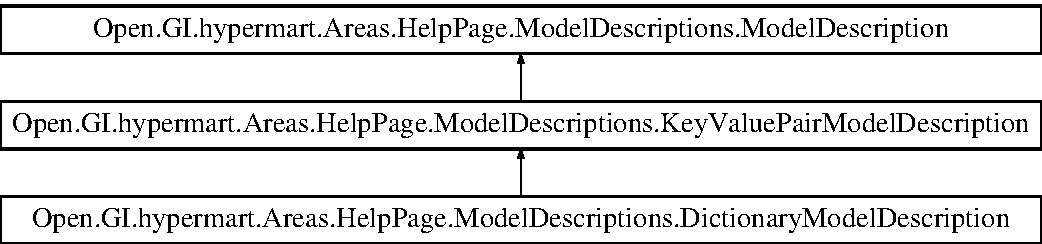
\includegraphics[height=3.000000cm]{class_open_1_1_g_i_1_1hypermart_1_1_areas_1_1_help_page_1_1_model_descriptions_1_1_dictionary_model_description}
\end{center}
\end{figure}
\subsection*{Additional Inherited Members}


\subsection{Detailed Description}


\begin{DoxySeeAlso}{See also}
\hyperlink{class_open_1_1_g_i_1_1hypermart_1_1_areas_1_1_help_page_1_1_model_descriptions_1_1_key_value_pair_model_description}{Open.\+G\+I.\+hypermart.\+Areas.\+Help\+Page.\+Model\+Descriptions.\+Key\+Value\+Pair\+Model\+Description}


\end{DoxySeeAlso}


Definition at line 7 of file Dictionary\+Model\+Description.\+cs.



The documentation for this class was generated from the following file\+:\begin{DoxyCompactItemize}
\item 
C\+:/\+Projects/\+App-\/\+Utility-\/\+Store/\+Open.\+G\+I.\+hypermart/\+Areas/\+Help\+Page/\+Model\+Descriptions/\hyperlink{_dictionary_model_description_8cs}{Dictionary\+Model\+Description.\+cs}\end{DoxyCompactItemize}

\hypertarget{class_open_1_1_g_i_1_1hypermart_1_1_controllers_1_1_download_controller}{}\section{Open.\+G\+I.\+hypermart.\+Controllers.\+Download\+Controller Class Reference}
\label{class_open_1_1_g_i_1_1hypermart_1_1_controllers_1_1_download_controller}\index{Open.\+G\+I.\+hypermart.\+Controllers.\+Download\+Controller@{Open.\+G\+I.\+hypermart.\+Controllers.\+Download\+Controller}}


Controller responsible for serving donwload files to the user.  


Inheritance diagram for Open.\+G\+I.\+hypermart.\+Controllers.\+Download\+Controller\+:\begin{figure}[H]
\begin{center}
\leavevmode
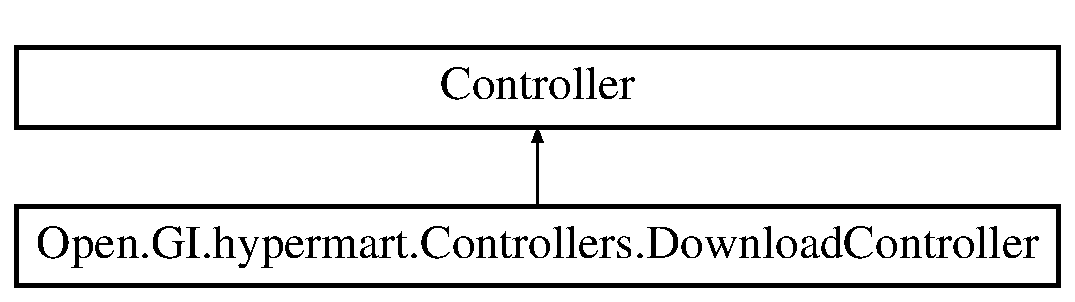
\includegraphics[height=2.000000cm]{class_open_1_1_g_i_1_1hypermart_1_1_controllers_1_1_download_controller}
\end{center}
\end{figure}
\subsection*{Public Member Functions}
\begin{DoxyCompactItemize}
\item 
File\+Result \hyperlink{class_open_1_1_g_i_1_1hypermart_1_1_controllers_1_1_download_controller_a272d3e80defa78e91555596d44891c47}{Download} (int id)
\begin{DoxyCompactList}\small\item\em Downloads the specified identifier. \end{DoxyCompactList}\end{DoxyCompactItemize}


\subsection{Detailed Description}
Controller responsible for serving donwload files to the user. 

\begin{DoxySeeAlso}{See also}
System.\+Web.\+Mvc.\+Controller


\end{DoxySeeAlso}


\subsection{Member Function Documentation}
\hypertarget{class_open_1_1_g_i_1_1hypermart_1_1_controllers_1_1_download_controller_a272d3e80defa78e91555596d44891c47}{}\label{class_open_1_1_g_i_1_1hypermart_1_1_controllers_1_1_download_controller_a272d3e80defa78e91555596d44891c47} 
\index{Open\+::\+G\+I\+::hypermart\+::\+Controllers\+::\+Download\+Controller@{Open\+::\+G\+I\+::hypermart\+::\+Controllers\+::\+Download\+Controller}!Download@{Download}}
\index{Download@{Download}!Open\+::\+G\+I\+::hypermart\+::\+Controllers\+::\+Download\+Controller@{Open\+::\+G\+I\+::hypermart\+::\+Controllers\+::\+Download\+Controller}}
\subsubsection{\texorpdfstring{Download()}{Download()}}
{\footnotesize\ttfamily File\+Result Open.\+G\+I.\+hypermart.\+Controllers.\+Download\+Controller.\+Download (\begin{DoxyParamCaption}\item[{int}]{id }\end{DoxyParamCaption})}



Downloads the specified identifier. 


\begin{DoxyParams}{Parameters}
{\em id} & The identifier.\\
\hline
\end{DoxyParams}
\begin{DoxyReturn}{Returns}

\end{DoxyReturn}

\begin{DoxyExceptions}{Exceptions}
{\em System.\+Web.\+Http\+Exception} & Cannot find file or Cannot find file -\/ can\textquotesingle{}t get remote link. \\
\hline
\end{DoxyExceptions}


The documentation for this class was generated from the following file\+:\begin{DoxyCompactItemize}
\item 
C\+:/\+Projects/\+App-\/\+Utility-\/\+Store/\+Open.\+G\+I.\+hypermart/\+Controllers/\hyperlink{_download_controller_8cs}{Download\+Controller.\+cs}\end{DoxyCompactItemize}

\section{Open.\+G\+I.\+hypermart.\+Helpers.\+Empty\+Controller Class Reference}
\label{class_open_1_1_g_i_1_1hypermart_1_1_helpers_1_1_empty_controller}\index{Open.\+G\+I.\+hypermart.\+Helpers.\+Empty\+Controller@{Open.\+G\+I.\+hypermart.\+Helpers.\+Empty\+Controller}}


Empty M\+VC Controller instance used to instantiate and provide a new Controller\+Context for the \doxyref{View\+Renderer}{p.}{class_open_1_1_g_i_1_1hypermart_1_1_helpers_1_1_view_renderer}  


Inheritance diagram for Open.\+G\+I.\+hypermart.\+Helpers.\+Empty\+Controller\+:\begin{figure}[H]
\begin{center}
\leavevmode
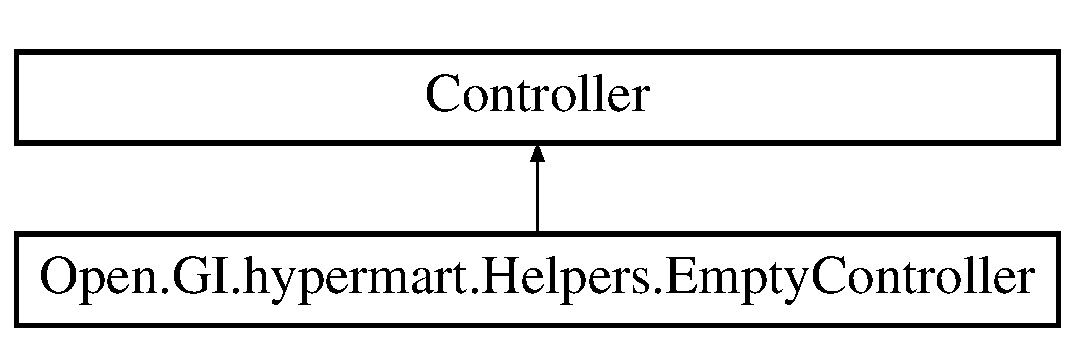
\includegraphics[height=2.000000cm]{class_open_1_1_g_i_1_1hypermart_1_1_helpers_1_1_empty_controller}
\end{center}
\end{figure}


\subsection{Detailed Description}
Empty M\+VC Controller instance used to instantiate and provide a new Controller\+Context for the \doxyref{View\+Renderer}{p.}{class_open_1_1_g_i_1_1hypermart_1_1_helpers_1_1_view_renderer} 



Definition at line 367 of file View\+Renderer.\+cs.



The documentation for this class was generated from the following file\+:\begin{DoxyCompactItemize}
\item 
C\+:/\+Projects/\+App-\/\+Utility-\/\+Store/\+Open.\+G\+I.\+hypermart/\+Helpers/\textbf{ View\+Renderer.\+cs}\end{DoxyCompactItemize}

\section{Open.\+G\+I.\+hypermart.\+Areas.\+Help\+Page.\+Model\+Descriptions.\+Enum\+Type\+Model\+Description Class Reference}
\label{class_open_1_1_g_i_1_1hypermart_1_1_areas_1_1_help_page_1_1_model_descriptions_1_1_enum_type_model_description}\index{Open.\+G\+I.\+hypermart.\+Areas.\+Help\+Page.\+Model\+Descriptions.\+Enum\+Type\+Model\+Description@{Open.\+G\+I.\+hypermart.\+Areas.\+Help\+Page.\+Model\+Descriptions.\+Enum\+Type\+Model\+Description}}


 


Inheritance diagram for Open.\+G\+I.\+hypermart.\+Areas.\+Help\+Page.\+Model\+Descriptions.\+Enum\+Type\+Model\+Description\+:\begin{figure}[H]
\begin{center}
\leavevmode
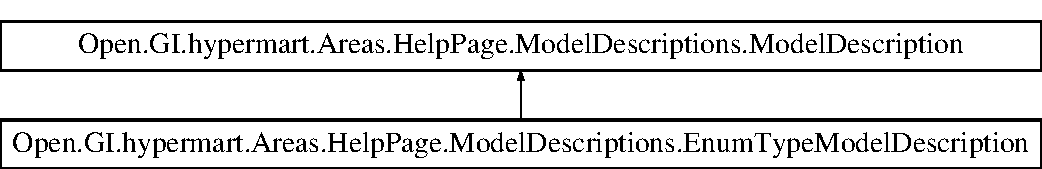
\includegraphics[height=2.000000cm]{class_open_1_1_g_i_1_1hypermart_1_1_areas_1_1_help_page_1_1_model_descriptions_1_1_enum_type_model_description}
\end{center}
\end{figure}
\subsection*{Public Member Functions}
\begin{DoxyCompactItemize}
\item 
\textbf{ Enum\+Type\+Model\+Description} ()
\begin{DoxyCompactList}\small\item\em Initializes a new instance of the \doxyref{Enum\+Type\+Model\+Description}{p.}{class_open_1_1_g_i_1_1hypermart_1_1_areas_1_1_help_page_1_1_model_descriptions_1_1_enum_type_model_description} class. \end{DoxyCompactList}\end{DoxyCompactItemize}
\subsection*{Properties}
\begin{DoxyCompactItemize}
\item 
Collection$<$ \textbf{ Enum\+Value\+Description} $>$ \textbf{ Values}\hspace{0.3cm}{\ttfamily  [get]}
\begin{DoxyCompactList}\small\item\em Gets the values. \end{DoxyCompactList}\end{DoxyCompactItemize}


\subsection{Detailed Description}


\begin{DoxySeeAlso}{See also}
\doxyref{Open.\+G\+I.\+hypermart.\+Areas.\+Help\+Page.\+Model\+Descriptions.\+Model\+Description}{p.}{class_open_1_1_g_i_1_1hypermart_1_1_areas_1_1_help_page_1_1_model_descriptions_1_1_model_description}


\end{DoxySeeAlso}


Definition at line 10 of file Enum\+Type\+Model\+Description.\+cs.



\subsection{Constructor \& Destructor Documentation}
\mbox{\label{class_open_1_1_g_i_1_1hypermart_1_1_areas_1_1_help_page_1_1_model_descriptions_1_1_enum_type_model_description_a77a337dadd9fdcee12869c7385bf51dc}} 
\index{Open\+::\+G\+I\+::hypermart\+::\+Areas\+::\+Help\+Page\+::\+Model\+Descriptions\+::\+Enum\+Type\+Model\+Description@{Open\+::\+G\+I\+::hypermart\+::\+Areas\+::\+Help\+Page\+::\+Model\+Descriptions\+::\+Enum\+Type\+Model\+Description}!Enum\+Type\+Model\+Description@{Enum\+Type\+Model\+Description}}
\index{Enum\+Type\+Model\+Description@{Enum\+Type\+Model\+Description}!Open\+::\+G\+I\+::hypermart\+::\+Areas\+::\+Help\+Page\+::\+Model\+Descriptions\+::\+Enum\+Type\+Model\+Description@{Open\+::\+G\+I\+::hypermart\+::\+Areas\+::\+Help\+Page\+::\+Model\+Descriptions\+::\+Enum\+Type\+Model\+Description}}
\subsubsection{Enum\+Type\+Model\+Description()}
{\footnotesize\ttfamily Open.\+G\+I.\+hypermart.\+Areas.\+Help\+Page.\+Model\+Descriptions.\+Enum\+Type\+Model\+Description.\+Enum\+Type\+Model\+Description (\begin{DoxyParamCaption}{ }\end{DoxyParamCaption})}



Initializes a new instance of the \doxyref{Enum\+Type\+Model\+Description}{p.}{class_open_1_1_g_i_1_1hypermart_1_1_areas_1_1_help_page_1_1_model_descriptions_1_1_enum_type_model_description} class. 



Definition at line 15 of file Enum\+Type\+Model\+Description.\+cs.



\subsection{Property Documentation}
\mbox{\label{class_open_1_1_g_i_1_1hypermart_1_1_areas_1_1_help_page_1_1_model_descriptions_1_1_enum_type_model_description_a7b42c1652865a638dd214ba6a1642819}} 
\index{Open\+::\+G\+I\+::hypermart\+::\+Areas\+::\+Help\+Page\+::\+Model\+Descriptions\+::\+Enum\+Type\+Model\+Description@{Open\+::\+G\+I\+::hypermart\+::\+Areas\+::\+Help\+Page\+::\+Model\+Descriptions\+::\+Enum\+Type\+Model\+Description}!Values@{Values}}
\index{Values@{Values}!Open\+::\+G\+I\+::hypermart\+::\+Areas\+::\+Help\+Page\+::\+Model\+Descriptions\+::\+Enum\+Type\+Model\+Description@{Open\+::\+G\+I\+::hypermart\+::\+Areas\+::\+Help\+Page\+::\+Model\+Descriptions\+::\+Enum\+Type\+Model\+Description}}
\subsubsection{Values}
{\footnotesize\ttfamily Collection$<$\textbf{ Enum\+Value\+Description}$>$ Open.\+G\+I.\+hypermart.\+Areas.\+Help\+Page.\+Model\+Descriptions.\+Enum\+Type\+Model\+Description.\+Values\hspace{0.3cm}{\ttfamily [get]}}



Gets the values. 

The values. 

Definition at line 26 of file Enum\+Type\+Model\+Description.\+cs.



The documentation for this class was generated from the following file\+:\begin{DoxyCompactItemize}
\item 
C\+:/\+Projects/\+App-\/\+Utility-\/\+Store/\+Open.\+G\+I.\+hypermart/\+Areas/\+Help\+Page/\+Model\+Descriptions/\textbf{ Enum\+Type\+Model\+Description.\+cs}\end{DoxyCompactItemize}

\hypertarget{class_open_1_1_g_i_1_1hypermart_1_1_areas_1_1_help_page_1_1_model_descriptions_1_1_enum_value_description}{}\section{Open.\+G\+I.\+hypermart.\+Areas.\+Help\+Page.\+Model\+Descriptions.\+Enum\+Value\+Description Class Reference}
\label{class_open_1_1_g_i_1_1hypermart_1_1_areas_1_1_help_page_1_1_model_descriptions_1_1_enum_value_description}\index{Open.\+G\+I.\+hypermart.\+Areas.\+Help\+Page.\+Model\+Descriptions.\+Enum\+Value\+Description@{Open.\+G\+I.\+hypermart.\+Areas.\+Help\+Page.\+Model\+Descriptions.\+Enum\+Value\+Description}}


 


\subsection*{Properties}
\begin{DoxyCompactItemize}
\item 
string \hyperlink{class_open_1_1_g_i_1_1hypermart_1_1_areas_1_1_help_page_1_1_model_descriptions_1_1_enum_value_description_a8e1e8adc9b367cdc6034e648067585c9}{Documentation}\hspace{0.3cm}{\ttfamily  \mbox{[}get, set\mbox{]}}
\begin{DoxyCompactList}\small\item\em Gets or sets the documentation. \end{DoxyCompactList}\item 
string \hyperlink{class_open_1_1_g_i_1_1hypermart_1_1_areas_1_1_help_page_1_1_model_descriptions_1_1_enum_value_description_a9a7f37f9e6c2a01c41a557b7a8e65d4e}{Name}\hspace{0.3cm}{\ttfamily  \mbox{[}get, set\mbox{]}}
\begin{DoxyCompactList}\small\item\em Gets or sets the name. \end{DoxyCompactList}\item 
string \hyperlink{class_open_1_1_g_i_1_1hypermart_1_1_areas_1_1_help_page_1_1_model_descriptions_1_1_enum_value_description_ab94229a6c9c5afad58abc04d705169f8}{Value}\hspace{0.3cm}{\ttfamily  \mbox{[}get, set\mbox{]}}
\begin{DoxyCompactList}\small\item\em Gets or sets the value. \end{DoxyCompactList}\end{DoxyCompactItemize}


\subsection{Detailed Description}




Definition at line 6 of file Enum\+Value\+Description.\+cs.



\subsection{Property Documentation}
\hypertarget{class_open_1_1_g_i_1_1hypermart_1_1_areas_1_1_help_page_1_1_model_descriptions_1_1_enum_value_description_a8e1e8adc9b367cdc6034e648067585c9}{}\index{Open\+::\+G\+I\+::hypermart\+::\+Areas\+::\+Help\+Page\+::\+Model\+Descriptions\+::\+Enum\+Value\+Description@{Open\+::\+G\+I\+::hypermart\+::\+Areas\+::\+Help\+Page\+::\+Model\+Descriptions\+::\+Enum\+Value\+Description}!Documentation@{Documentation}}
\index{Documentation@{Documentation}!Open\+::\+G\+I\+::hypermart\+::\+Areas\+::\+Help\+Page\+::\+Model\+Descriptions\+::\+Enum\+Value\+Description@{Open\+::\+G\+I\+::hypermart\+::\+Areas\+::\+Help\+Page\+::\+Model\+Descriptions\+::\+Enum\+Value\+Description}}
\subsubsection[{Documentation}]{\setlength{\rightskip}{0pt plus 5cm}string Open.\+G\+I.\+hypermart.\+Areas.\+Help\+Page.\+Model\+Descriptions.\+Enum\+Value\+Description.\+Documentation\hspace{0.3cm}{\ttfamily [get]}, {\ttfamily [set]}}\label{class_open_1_1_g_i_1_1hypermart_1_1_areas_1_1_help_page_1_1_model_descriptions_1_1_enum_value_description_a8e1e8adc9b367cdc6034e648067585c9}


Gets or sets the documentation. 

The documentation. 

Definition at line 14 of file Enum\+Value\+Description.\+cs.

\hypertarget{class_open_1_1_g_i_1_1hypermart_1_1_areas_1_1_help_page_1_1_model_descriptions_1_1_enum_value_description_a9a7f37f9e6c2a01c41a557b7a8e65d4e}{}\index{Open\+::\+G\+I\+::hypermart\+::\+Areas\+::\+Help\+Page\+::\+Model\+Descriptions\+::\+Enum\+Value\+Description@{Open\+::\+G\+I\+::hypermart\+::\+Areas\+::\+Help\+Page\+::\+Model\+Descriptions\+::\+Enum\+Value\+Description}!Name@{Name}}
\index{Name@{Name}!Open\+::\+G\+I\+::hypermart\+::\+Areas\+::\+Help\+Page\+::\+Model\+Descriptions\+::\+Enum\+Value\+Description@{Open\+::\+G\+I\+::hypermart\+::\+Areas\+::\+Help\+Page\+::\+Model\+Descriptions\+::\+Enum\+Value\+Description}}
\subsubsection[{Name}]{\setlength{\rightskip}{0pt plus 5cm}string Open.\+G\+I.\+hypermart.\+Areas.\+Help\+Page.\+Model\+Descriptions.\+Enum\+Value\+Description.\+Name\hspace{0.3cm}{\ttfamily [get]}, {\ttfamily [set]}}\label{class_open_1_1_g_i_1_1hypermart_1_1_areas_1_1_help_page_1_1_model_descriptions_1_1_enum_value_description_a9a7f37f9e6c2a01c41a557b7a8e65d4e}


Gets or sets the name. 

The name. 

Definition at line 22 of file Enum\+Value\+Description.\+cs.

\hypertarget{class_open_1_1_g_i_1_1hypermart_1_1_areas_1_1_help_page_1_1_model_descriptions_1_1_enum_value_description_ab94229a6c9c5afad58abc04d705169f8}{}\index{Open\+::\+G\+I\+::hypermart\+::\+Areas\+::\+Help\+Page\+::\+Model\+Descriptions\+::\+Enum\+Value\+Description@{Open\+::\+G\+I\+::hypermart\+::\+Areas\+::\+Help\+Page\+::\+Model\+Descriptions\+::\+Enum\+Value\+Description}!Value@{Value}}
\index{Value@{Value}!Open\+::\+G\+I\+::hypermart\+::\+Areas\+::\+Help\+Page\+::\+Model\+Descriptions\+::\+Enum\+Value\+Description@{Open\+::\+G\+I\+::hypermart\+::\+Areas\+::\+Help\+Page\+::\+Model\+Descriptions\+::\+Enum\+Value\+Description}}
\subsubsection[{Value}]{\setlength{\rightskip}{0pt plus 5cm}string Open.\+G\+I.\+hypermart.\+Areas.\+Help\+Page.\+Model\+Descriptions.\+Enum\+Value\+Description.\+Value\hspace{0.3cm}{\ttfamily [get]}, {\ttfamily [set]}}\label{class_open_1_1_g_i_1_1hypermart_1_1_areas_1_1_help_page_1_1_model_descriptions_1_1_enum_value_description_ab94229a6c9c5afad58abc04d705169f8}


Gets or sets the value. 

The value. 

Definition at line 30 of file Enum\+Value\+Description.\+cs.



The documentation for this class was generated from the following file\+:\begin{DoxyCompactItemize}
\item 
C\+:/\+Projects/\+App-\/\+Utility-\/\+Store/\+Open.\+G\+I.\+hypermart/\+Areas/\+Help\+Page/\+Model\+Descriptions/\hyperlink{_enum_value_description_8cs}{Enum\+Value\+Description.\+cs}\end{DoxyCompactItemize}

\hypertarget{class_open_1_1_g_i_1_1hypermart_1_1_controllers_1_1_fake_controller}{}\section{Open.\+G\+I.\+hypermart.\+Controllers.\+Fake\+Controller Class Reference}
\label{class_open_1_1_g_i_1_1hypermart_1_1_controllers_1_1_fake_controller}\index{Open.\+G\+I.\+hypermart.\+Controllers.\+Fake\+Controller@{Open.\+G\+I.\+hypermart.\+Controllers.\+Fake\+Controller}}


Controller for returning Errors  


Inheritance diagram for Open.\+G\+I.\+hypermart.\+Controllers.\+Fake\+Controller\+:\begin{figure}[H]
\begin{center}
\leavevmode
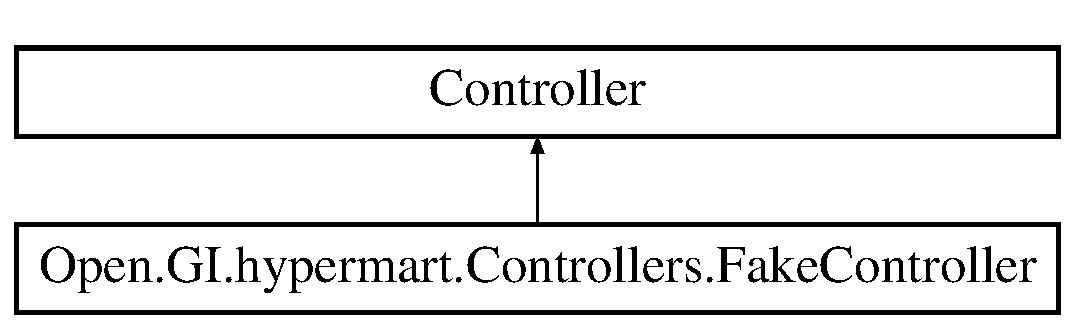
\includegraphics[height=2.000000cm]{class_open_1_1_g_i_1_1hypermart_1_1_controllers_1_1_fake_controller}
\end{center}
\end{figure}
\subsection*{Public Member Functions}
\begin{DoxyCompactItemize}
\item 
Action\+Result \hyperlink{class_open_1_1_g_i_1_1hypermart_1_1_controllers_1_1_fake_controller_a783fcc0fd5e686066951dc93380d02bd}{Index} ()
\begin{DoxyCompactList}\small\item\em Indexes this instance. \end{DoxyCompactList}\end{DoxyCompactItemize}


\subsection{Detailed Description}
Controller for returning Errors 

\begin{DoxySeeAlso}{See also}
System.\+Web.\+Mvc.\+Controller


\end{DoxySeeAlso}


\subsection{Member Function Documentation}
\hypertarget{class_open_1_1_g_i_1_1hypermart_1_1_controllers_1_1_fake_controller_a783fcc0fd5e686066951dc93380d02bd}{}\label{class_open_1_1_g_i_1_1hypermart_1_1_controllers_1_1_fake_controller_a783fcc0fd5e686066951dc93380d02bd} 
\index{Open\+::\+G\+I\+::hypermart\+::\+Controllers\+::\+Fake\+Controller@{Open\+::\+G\+I\+::hypermart\+::\+Controllers\+::\+Fake\+Controller}!Index@{Index}}
\index{Index@{Index}!Open\+::\+G\+I\+::hypermart\+::\+Controllers\+::\+Fake\+Controller@{Open\+::\+G\+I\+::hypermart\+::\+Controllers\+::\+Fake\+Controller}}
\subsubsection{\texorpdfstring{Index()}{Index()}}
{\footnotesize\ttfamily Action\+Result Open.\+G\+I.\+hypermart.\+Controllers.\+Fake\+Controller.\+Index (\begin{DoxyParamCaption}{ }\end{DoxyParamCaption})}



Indexes this instance. 

\begin{DoxyReturn}{Returns}

\end{DoxyReturn}


The documentation for this class was generated from the following file\+:\begin{DoxyCompactItemize}
\item 
C\+:/\+Projects/\+App-\/\+Utility-\/\+Store/\+Open.\+G\+I.\+hypermart/\+Controllers/\hyperlink{_fake_controller_8cs}{Fake\+Controller.\+cs}\end{DoxyCompactItemize}

\section{Open.\+G\+I.\+hypermart.\+Models.\+File Class Reference}
\label{class_open_1_1_g_i_1_1hypermart_1_1_models_1_1_file}\index{Open.\+G\+I.\+hypermart.\+Models.\+File@{Open.\+G\+I.\+hypermart.\+Models.\+File}}


Model Class representing a \doxyref{File}{p.}{class_open_1_1_g_i_1_1hypermart_1_1_models_1_1_file}.  


\subsection*{Public Member Functions}
\begin{DoxyCompactItemize}
\item 
\textbf{ File} ()
\begin{DoxyCompactList}\small\item\em Initializes a new instance of the \doxyref{File}{p.}{class_open_1_1_g_i_1_1hypermart_1_1_models_1_1_file} class. \end{DoxyCompactList}\item 
\textbf{ File} ()
\end{DoxyCompactItemize}
\subsection*{Properties}
\begin{DoxyCompactItemize}
\item 
int \textbf{ ID}\hspace{0.3cm}{\ttfamily  [get, set]}
\begin{DoxyCompactList}\small\item\em Gets or sets the identifier. \end{DoxyCompactList}\item 
\textbf{ storage\+Type} \textbf{ Storage\+Type}\hspace{0.3cm}{\ttfamily  [get, set]}
\begin{DoxyCompactList}\small\item\em Gets or sets the type of the storage. \end{DoxyCompactList}\item 
string \textbf{ File\+Name}\hspace{0.3cm}{\ttfamily  [get, set]}
\begin{DoxyCompactList}\small\item\em Gets or sets the name of the file. \end{DoxyCompactList}\item 
byte [$\,$] \textbf{ B\+L\+OB}\hspace{0.3cm}{\ttfamily  [get, set]}
\begin{DoxyCompactList}\small\item\em Gets or sets the B\+L\+OB. \end{DoxyCompactList}\item 
string \textbf{ Link}\hspace{0.3cm}{\ttfamily  [get, set]}
\begin{DoxyCompactList}\small\item\em Gets or sets the link. \end{DoxyCompactList}\item 
string \textbf{ Version}\hspace{0.3cm}{\ttfamily  [get, set]}
\begin{DoxyCompactList}\small\item\em Gets or sets the version. \end{DoxyCompactList}\item 
int \textbf{ Product\+ID}\hspace{0.3cm}{\ttfamily  [get, set]}
\begin{DoxyCompactList}\small\item\em Gets or sets the product identifier. \end{DoxyCompactList}\item 
\textbf{ Product} \textbf{ Product}\hspace{0.3cm}{\ttfamily  [get, set]}
\begin{DoxyCompactList}\small\item\em Gets or sets the product. \end{DoxyCompactList}\item 
virtual I\+Collection$<$ \textbf{ Platform} $>$ \textbf{ Platforms}\hspace{0.3cm}{\ttfamily  [get, set]}
\begin{DoxyCompactList}\small\item\em Gets or sets the platforms. \end{DoxyCompactList}\item 
int \textbf{ Storage\+Type}\hspace{0.3cm}{\ttfamily  [get, set]}
\item 
Nullable$<$ int $>$ \textbf{ Product\+ID}\hspace{0.3cm}{\ttfamily  [get, set]}
\item 
virtual \textbf{ Product} \textbf{ Product}\hspace{0.3cm}{\ttfamily  [get, set]}
\item 
virtual I\+Collection$<$ \textbf{ File\+Platform} $>$ \textbf{ File\+Platforms}\hspace{0.3cm}{\ttfamily  [get, set]}
\end{DoxyCompactItemize}


\subsection{Detailed Description}
Model Class representing a \doxyref{File}{p.}{class_open_1_1_g_i_1_1hypermart_1_1_models_1_1_file}. 



Definition at line 12 of file File.\+cs.



\subsection{Constructor \& Destructor Documentation}
\mbox{\label{class_open_1_1_g_i_1_1hypermart_1_1_models_1_1_file_a6834fcf6e0ea0428dc2decfaa974f8d2}} 
\index{Open\+::\+G\+I\+::hypermart\+::\+Models\+::\+File@{Open\+::\+G\+I\+::hypermart\+::\+Models\+::\+File}!File@{File}}
\index{File@{File}!Open\+::\+G\+I\+::hypermart\+::\+Models\+::\+File@{Open\+::\+G\+I\+::hypermart\+::\+Models\+::\+File}}
\subsubsection{File()\hspace{0.1cm}{\footnotesize\ttfamily [1/2]}}
{\footnotesize\ttfamily Open.\+G\+I.\+hypermart.\+Models.\+File.\+File (\begin{DoxyParamCaption}{ }\end{DoxyParamCaption})}



Initializes a new instance of the \doxyref{File}{p.}{class_open_1_1_g_i_1_1hypermart_1_1_models_1_1_file} class. 



Definition at line 18 of file File.\+cs.

\mbox{\label{class_open_1_1_g_i_1_1hypermart_1_1_models_1_1_file_a6834fcf6e0ea0428dc2decfaa974f8d2}} 
\index{Open\+::\+G\+I\+::hypermart\+::\+Models\+::\+File@{Open\+::\+G\+I\+::hypermart\+::\+Models\+::\+File}!File@{File}}
\index{File@{File}!Open\+::\+G\+I\+::hypermart\+::\+Models\+::\+File@{Open\+::\+G\+I\+::hypermart\+::\+Models\+::\+File}}
\subsubsection{File()\hspace{0.1cm}{\footnotesize\ttfamily [2/2]}}
{\footnotesize\ttfamily Open.\+G\+I.\+hypermart.\+Models.\+File.\+File (\begin{DoxyParamCaption}{ }\end{DoxyParamCaption})}



Definition at line 18 of file File.\+cs.



\subsection{Property Documentation}
\mbox{\label{class_open_1_1_g_i_1_1hypermart_1_1_models_1_1_file_acfdfc6e64338fc14a71994e5d7aa5111}} 
\index{Open\+::\+G\+I\+::hypermart\+::\+Models\+::\+File@{Open\+::\+G\+I\+::hypermart\+::\+Models\+::\+File}!B\+L\+OB@{B\+L\+OB}}
\index{B\+L\+OB@{B\+L\+OB}!Open\+::\+G\+I\+::hypermart\+::\+Models\+::\+File@{Open\+::\+G\+I\+::hypermart\+::\+Models\+::\+File}}
\subsubsection{B\+L\+OB}
{\footnotesize\ttfamily byte [$\,$] Open.\+G\+I.\+hypermart.\+Models.\+File.\+B\+L\+OB\hspace{0.3cm}{\ttfamily [get]}, {\ttfamily [set]}}



Gets or sets the B\+L\+OB. 

The B\+L\+OB. 

Definition at line 53 of file File.\+cs.

\mbox{\label{class_open_1_1_g_i_1_1hypermart_1_1_models_1_1_file_a5675dd150dd5ca0de9bc6755fe6c45ad}} 
\index{Open\+::\+G\+I\+::hypermart\+::\+Models\+::\+File@{Open\+::\+G\+I\+::hypermart\+::\+Models\+::\+File}!File\+Name@{File\+Name}}
\index{File\+Name@{File\+Name}!Open\+::\+G\+I\+::hypermart\+::\+Models\+::\+File@{Open\+::\+G\+I\+::hypermart\+::\+Models\+::\+File}}
\subsubsection{File\+Name}
{\footnotesize\ttfamily string Open.\+G\+I.\+hypermart.\+Models.\+File.\+File\+Name\hspace{0.3cm}{\ttfamily [get]}, {\ttfamily [set]}}



Gets or sets the name of the file. 

The name of the file. 

Definition at line 45 of file File.\+cs.

\mbox{\label{class_open_1_1_g_i_1_1hypermart_1_1_models_1_1_file_ac075b378d09c288deda822c0ea6b854c}} 
\index{Open\+::\+G\+I\+::hypermart\+::\+Models\+::\+File@{Open\+::\+G\+I\+::hypermart\+::\+Models\+::\+File}!File\+Platforms@{File\+Platforms}}
\index{File\+Platforms@{File\+Platforms}!Open\+::\+G\+I\+::hypermart\+::\+Models\+::\+File@{Open\+::\+G\+I\+::hypermart\+::\+Models\+::\+File}}
\subsubsection{File\+Platforms}
{\footnotesize\ttfamily virtual I\+Collection$<$\textbf{ File\+Platform}$>$ Open.\+G\+I.\+hypermart.\+Models.\+File.\+File\+Platforms\hspace{0.3cm}{\ttfamily [get]}, {\ttfamily [set]}}



Definition at line 33 of file File.\+cs.

\mbox{\label{class_open_1_1_g_i_1_1hypermart_1_1_models_1_1_file_ade215e549b777e8f30cfa19ec28cff96}} 
\index{Open\+::\+G\+I\+::hypermart\+::\+Models\+::\+File@{Open\+::\+G\+I\+::hypermart\+::\+Models\+::\+File}!ID@{ID}}
\index{ID@{ID}!Open\+::\+G\+I\+::hypermart\+::\+Models\+::\+File@{Open\+::\+G\+I\+::hypermart\+::\+Models\+::\+File}}
\subsubsection{ID}
{\footnotesize\ttfamily int Open.\+G\+I.\+hypermart.\+Models.\+File.\+ID\hspace{0.3cm}{\ttfamily [get]}, {\ttfamily [set]}}



Gets or sets the identifier. 

The identifier. 

Definition at line 29 of file File.\+cs.

\mbox{\label{class_open_1_1_g_i_1_1hypermart_1_1_models_1_1_file_a47b36d33252b1a1f58bee02a94d11dd5}} 
\index{Open\+::\+G\+I\+::hypermart\+::\+Models\+::\+File@{Open\+::\+G\+I\+::hypermart\+::\+Models\+::\+File}!Link@{Link}}
\index{Link@{Link}!Open\+::\+G\+I\+::hypermart\+::\+Models\+::\+File@{Open\+::\+G\+I\+::hypermart\+::\+Models\+::\+File}}
\subsubsection{Link}
{\footnotesize\ttfamily string Open.\+G\+I.\+hypermart.\+Models.\+File.\+Link\hspace{0.3cm}{\ttfamily [get]}, {\ttfamily [set]}}



Gets or sets the link. 

The link. 

Definition at line 61 of file File.\+cs.

\mbox{\label{class_open_1_1_g_i_1_1hypermart_1_1_models_1_1_file_a7cf38ed851b70df6af9b0606c4d744ed}} 
\index{Open\+::\+G\+I\+::hypermart\+::\+Models\+::\+File@{Open\+::\+G\+I\+::hypermart\+::\+Models\+::\+File}!Platforms@{Platforms}}
\index{Platforms@{Platforms}!Open\+::\+G\+I\+::hypermart\+::\+Models\+::\+File@{Open\+::\+G\+I\+::hypermart\+::\+Models\+::\+File}}
\subsubsection{Platforms}
{\footnotesize\ttfamily virtual I\+Collection$<$\textbf{ Platform}$>$ Open.\+G\+I.\+hypermart.\+Models.\+File.\+Platforms\hspace{0.3cm}{\ttfamily [get]}, {\ttfamily [set]}}



Gets or sets the platforms. 

The platforms. 

Definition at line 95 of file File.\+cs.

\mbox{\label{class_open_1_1_g_i_1_1hypermart_1_1_models_1_1_file_a7a2d45936082be844aa8528b298a2d6a}} 
\index{Open\+::\+G\+I\+::hypermart\+::\+Models\+::\+File@{Open\+::\+G\+I\+::hypermart\+::\+Models\+::\+File}!Product@{Product}}
\index{Product@{Product}!Open\+::\+G\+I\+::hypermart\+::\+Models\+::\+File@{Open\+::\+G\+I\+::hypermart\+::\+Models\+::\+File}}
\subsubsection{Product\hspace{0.1cm}{\footnotesize\ttfamily [1/2]}}
{\footnotesize\ttfamily virtual \textbf{ Product} Open.\+G\+I.\+hypermart.\+Models.\+File.\+Product\hspace{0.3cm}{\ttfamily [get]}, {\ttfamily [set]}}



Definition at line 31 of file File.\+cs.

\mbox{\label{class_open_1_1_g_i_1_1hypermart_1_1_models_1_1_file_a4b8d3f1af1802269e9e06285f9bf81b3}} 
\index{Open\+::\+G\+I\+::hypermart\+::\+Models\+::\+File@{Open\+::\+G\+I\+::hypermart\+::\+Models\+::\+File}!Product@{Product}}
\index{Product@{Product}!Open\+::\+G\+I\+::hypermart\+::\+Models\+::\+File@{Open\+::\+G\+I\+::hypermart\+::\+Models\+::\+File}}
\subsubsection{Product\hspace{0.1cm}{\footnotesize\ttfamily [2/2]}}
{\footnotesize\ttfamily \textbf{ Product} Open.\+G\+I.\+hypermart.\+Models.\+File.\+Product\hspace{0.3cm}{\ttfamily [get]}, {\ttfamily [set]}}



Gets or sets the product. 

The product. 

Definition at line 86 of file File.\+cs.

\mbox{\label{class_open_1_1_g_i_1_1hypermart_1_1_models_1_1_file_ad0b974d38df4491ce90d1d5e884a56a8}} 
\index{Open\+::\+G\+I\+::hypermart\+::\+Models\+::\+File@{Open\+::\+G\+I\+::hypermart\+::\+Models\+::\+File}!Product\+ID@{Product\+ID}}
\index{Product\+ID@{Product\+ID}!Open\+::\+G\+I\+::hypermart\+::\+Models\+::\+File@{Open\+::\+G\+I\+::hypermart\+::\+Models\+::\+File}}
\subsubsection{Product\+ID\hspace{0.1cm}{\footnotesize\ttfamily [1/2]}}
{\footnotesize\ttfamily Nullable$<$int$>$ Open.\+G\+I.\+hypermart.\+Models.\+File.\+Product\+ID\hspace{0.3cm}{\ttfamily [get]}, {\ttfamily [set]}}



Definition at line 29 of file File.\+cs.

\mbox{\label{class_open_1_1_g_i_1_1hypermart_1_1_models_1_1_file_a7f0a3da01808662b23635d9b9b6f6848}} 
\index{Open\+::\+G\+I\+::hypermart\+::\+Models\+::\+File@{Open\+::\+G\+I\+::hypermart\+::\+Models\+::\+File}!Product\+ID@{Product\+ID}}
\index{Product\+ID@{Product\+ID}!Open\+::\+G\+I\+::hypermart\+::\+Models\+::\+File@{Open\+::\+G\+I\+::hypermart\+::\+Models\+::\+File}}
\subsubsection{Product\+ID\hspace{0.1cm}{\footnotesize\ttfamily [2/2]}}
{\footnotesize\ttfamily int Open.\+G\+I.\+hypermart.\+Models.\+File.\+Product\+ID\hspace{0.3cm}{\ttfamily [get]}, {\ttfamily [set]}}



Gets or sets the product identifier. 

The product identifier. 

Definition at line 78 of file File.\+cs.

\mbox{\label{class_open_1_1_g_i_1_1hypermart_1_1_models_1_1_file_ab4ac8af085696918a7a4e1765639066d}} 
\index{Open\+::\+G\+I\+::hypermart\+::\+Models\+::\+File@{Open\+::\+G\+I\+::hypermart\+::\+Models\+::\+File}!Storage\+Type@{Storage\+Type}}
\index{Storage\+Type@{Storage\+Type}!Open\+::\+G\+I\+::hypermart\+::\+Models\+::\+File@{Open\+::\+G\+I\+::hypermart\+::\+Models\+::\+File}}
\subsubsection{Storage\+Type\hspace{0.1cm}{\footnotesize\ttfamily [1/2]}}
{\footnotesize\ttfamily int Open.\+G\+I.\+hypermart.\+Models.\+File.\+Storage\+Type\hspace{0.3cm}{\ttfamily [get]}, {\ttfamily [set]}}



Definition at line 24 of file File.\+cs.

\mbox{\label{class_open_1_1_g_i_1_1hypermart_1_1_models_1_1_file_a4d6910e1f3277beb5b50309e8139a356}} 
\index{Open\+::\+G\+I\+::hypermart\+::\+Models\+::\+File@{Open\+::\+G\+I\+::hypermart\+::\+Models\+::\+File}!Storage\+Type@{Storage\+Type}}
\index{Storage\+Type@{Storage\+Type}!Open\+::\+G\+I\+::hypermart\+::\+Models\+::\+File@{Open\+::\+G\+I\+::hypermart\+::\+Models\+::\+File}}
\subsubsection{Storage\+Type\hspace{0.1cm}{\footnotesize\ttfamily [2/2]}}
{\footnotesize\ttfamily \textbf{ storage\+Type} Open.\+G\+I.\+hypermart.\+Models.\+File.\+Storage\+Type\hspace{0.3cm}{\ttfamily [get]}, {\ttfamily [set]}}



Gets or sets the type of the storage. 

The type of the storage. 

Definition at line 37 of file File.\+cs.

\mbox{\label{class_open_1_1_g_i_1_1hypermart_1_1_models_1_1_file_a59b1cbe55394fce55d55200ea7e55cae}} 
\index{Open\+::\+G\+I\+::hypermart\+::\+Models\+::\+File@{Open\+::\+G\+I\+::hypermart\+::\+Models\+::\+File}!Version@{Version}}
\index{Version@{Version}!Open\+::\+G\+I\+::hypermart\+::\+Models\+::\+File@{Open\+::\+G\+I\+::hypermart\+::\+Models\+::\+File}}
\subsubsection{Version}
{\footnotesize\ttfamily string Open.\+G\+I.\+hypermart.\+Models.\+File.\+Version\hspace{0.3cm}{\ttfamily [get]}, {\ttfamily [set]}}



Gets or sets the version. 

The version. 

Definition at line 70 of file File.\+cs.



The documentation for this class was generated from the following file\+:\begin{DoxyCompactItemize}
\item 
C\+:/\+Projects/\+App-\/\+Utility-\/\+Store/\+Open.\+G\+I.\+hypermart/\+Models/\textbf{ File.\+cs}\end{DoxyCompactItemize}

\hypertarget{class_open_1_1_g_i_1_1hypermart_1_1_data_transformation_objects_1_1_file_d_t_o}{}\section{Open.\+G\+I.\+hypermart.\+Data\+Transformation\+Objects.\+File\+D\+TO Class Reference}
\label{class_open_1_1_g_i_1_1hypermart_1_1_data_transformation_objects_1_1_file_d_t_o}\index{Open.\+G\+I.\+hypermart.\+Data\+Transformation\+Objects.\+File\+D\+TO@{Open.\+G\+I.\+hypermart.\+Data\+Transformation\+Objects.\+File\+D\+TO}}


 


\subsection*{Public Member Functions}
\begin{DoxyCompactItemize}
\item 
\hyperlink{class_open_1_1_g_i_1_1hypermart_1_1_data_transformation_objects_1_1_file_d_t_o_ae0da87388dbf076d2aa151cce63c81a8}{File\+D\+TO} ()
\begin{DoxyCompactList}\small\item\em Initializes a new instance of the \hyperlink{class_open_1_1_g_i_1_1hypermart_1_1_data_transformation_objects_1_1_file_d_t_o}{File\+D\+TO} class. \end{DoxyCompactList}\item 
\hyperlink{class_open_1_1_g_i_1_1hypermart_1_1_data_transformation_objects_1_1_file_d_t_o_add1a3ae47dca46ed24d3d8dda310a3a2}{File\+D\+TO} (\hyperlink{class_open_1_1_g_i_1_1hypermart_1_1_models_1_1_file}{File} \hyperlink{class_open_1_1_g_i_1_1hypermart_1_1_models_1_1_file}{File})
\begin{DoxyCompactList}\small\item\em Initializes a new instance of the \hyperlink{class_open_1_1_g_i_1_1hypermart_1_1_data_transformation_objects_1_1_file_d_t_o}{File\+D\+TO} class. \end{DoxyCompactList}\end{DoxyCompactItemize}
\subsection*{Properties}
\begin{DoxyCompactItemize}
\item 
int \hyperlink{class_open_1_1_g_i_1_1hypermart_1_1_data_transformation_objects_1_1_file_d_t_o_ab187e7f070650067d055de8f707e1eed}{ID}\hspace{0.3cm}{\ttfamily  \mbox{[}get, set\mbox{]}}
\begin{DoxyCompactList}\small\item\em Gets or sets the identifier. \end{DoxyCompactList}\item 
\hyperlink{namespace_open_1_1_g_i_1_1hypermart_1_1_models_a21c5ffa7da75ad8a6d2b04798113f9db}{storage\+Type} \hyperlink{class_open_1_1_g_i_1_1hypermart_1_1_data_transformation_objects_1_1_file_d_t_o_a4563713ee116eb1163eaac1f242b395f}{Storage\+Type}\hspace{0.3cm}{\ttfamily  \mbox{[}get, set\mbox{]}}
\begin{DoxyCompactList}\small\item\em Gets or sets the type of the storage. \end{DoxyCompactList}\item 
string \hyperlink{class_open_1_1_g_i_1_1hypermart_1_1_data_transformation_objects_1_1_file_d_t_o_a55fb34aacab9513037108ff3f1d287a8}{File\+Name}\hspace{0.3cm}{\ttfamily  \mbox{[}get, set\mbox{]}}
\begin{DoxyCompactList}\small\item\em Gets or sets the name of the file. \end{DoxyCompactList}\item 
byte \mbox{[}$\,$\mbox{]} \hyperlink{class_open_1_1_g_i_1_1hypermart_1_1_data_transformation_objects_1_1_file_d_t_o_af2ebb686a878cb8342e76648d048f19a}{B\+L\+OB}\hspace{0.3cm}{\ttfamily  \mbox{[}get, set\mbox{]}}
\begin{DoxyCompactList}\small\item\em Gets or sets the B\+L\+OB. \end{DoxyCompactList}\item 
string \hyperlink{class_open_1_1_g_i_1_1hypermart_1_1_data_transformation_objects_1_1_file_d_t_o_af58091e5ba2e9fde7db92f08dc4d3a41}{Link}\hspace{0.3cm}{\ttfamily  \mbox{[}get, set\mbox{]}}
\begin{DoxyCompactList}\small\item\em Gets or sets the link. \end{DoxyCompactList}\item 
string \hyperlink{class_open_1_1_g_i_1_1hypermart_1_1_data_transformation_objects_1_1_file_d_t_o_ac55a6e7062078277eed54e42b7c29d73}{Version}\hspace{0.3cm}{\ttfamily  \mbox{[}get, set\mbox{]}}
\begin{DoxyCompactList}\small\item\em Gets or sets the version. \end{DoxyCompactList}\item 
int \hyperlink{class_open_1_1_g_i_1_1hypermart_1_1_data_transformation_objects_1_1_file_d_t_o_abd8d9083fbb95dac1e2781f2a8d4f8e9}{Product\+ID}\hspace{0.3cm}{\ttfamily  \mbox{[}get, set\mbox{]}}
\begin{DoxyCompactList}\small\item\em Gets or sets the product identifier. \end{DoxyCompactList}\item 
virtual \hyperlink{class_open_1_1_g_i_1_1hypermart_1_1_models_1_1_product}{Product} \hyperlink{class_open_1_1_g_i_1_1hypermart_1_1_data_transformation_objects_1_1_file_d_t_o_aa587dd986d4c6d62d8bf5520d3a48e79}{Product}\hspace{0.3cm}{\ttfamily  \mbox{[}get, set\mbox{]}}
\begin{DoxyCompactList}\small\item\em Gets or sets the product. \end{DoxyCompactList}\item 
virtual I\+Collection$<$ \hyperlink{class_open_1_1_g_i_1_1hypermart_1_1_models_1_1_platform}{Platform} $>$ \hyperlink{class_open_1_1_g_i_1_1hypermart_1_1_data_transformation_objects_1_1_file_d_t_o_a784824c36cab74d3bc03a8ae55d9a62a}{Platforms}\hspace{0.3cm}{\ttfamily  \mbox{[}get, set\mbox{]}}
\begin{DoxyCompactList}\small\item\em Gets or sets the platforms. \end{DoxyCompactList}\end{DoxyCompactItemize}


\subsection{Detailed Description}




\subsection{Constructor \& Destructor Documentation}
\hypertarget{class_open_1_1_g_i_1_1hypermart_1_1_data_transformation_objects_1_1_file_d_t_o_ae0da87388dbf076d2aa151cce63c81a8}{}\label{class_open_1_1_g_i_1_1hypermart_1_1_data_transformation_objects_1_1_file_d_t_o_ae0da87388dbf076d2aa151cce63c81a8} 
\index{Open\+::\+G\+I\+::hypermart\+::\+Data\+Transformation\+Objects\+::\+File\+D\+TO@{Open\+::\+G\+I\+::hypermart\+::\+Data\+Transformation\+Objects\+::\+File\+D\+TO}!File\+D\+TO@{File\+D\+TO}}
\index{File\+D\+TO@{File\+D\+TO}!Open\+::\+G\+I\+::hypermart\+::\+Data\+Transformation\+Objects\+::\+File\+D\+TO@{Open\+::\+G\+I\+::hypermart\+::\+Data\+Transformation\+Objects\+::\+File\+D\+TO}}
\subsubsection{\texorpdfstring{File\+D\+T\+O()}{FileDTO()}\hspace{0.1cm}{\footnotesize\ttfamily [1/2]}}
{\footnotesize\ttfamily Open.\+G\+I.\+hypermart.\+Data\+Transformation\+Objects.\+File\+D\+T\+O.\+File\+D\+TO (\begin{DoxyParamCaption}{ }\end{DoxyParamCaption})}



Initializes a new instance of the \hyperlink{class_open_1_1_g_i_1_1hypermart_1_1_data_transformation_objects_1_1_file_d_t_o}{File\+D\+TO} class. 

\hypertarget{class_open_1_1_g_i_1_1hypermart_1_1_data_transformation_objects_1_1_file_d_t_o_add1a3ae47dca46ed24d3d8dda310a3a2}{}\label{class_open_1_1_g_i_1_1hypermart_1_1_data_transformation_objects_1_1_file_d_t_o_add1a3ae47dca46ed24d3d8dda310a3a2} 
\index{Open\+::\+G\+I\+::hypermart\+::\+Data\+Transformation\+Objects\+::\+File\+D\+TO@{Open\+::\+G\+I\+::hypermart\+::\+Data\+Transformation\+Objects\+::\+File\+D\+TO}!File\+D\+TO@{File\+D\+TO}}
\index{File\+D\+TO@{File\+D\+TO}!Open\+::\+G\+I\+::hypermart\+::\+Data\+Transformation\+Objects\+::\+File\+D\+TO@{Open\+::\+G\+I\+::hypermart\+::\+Data\+Transformation\+Objects\+::\+File\+D\+TO}}
\subsubsection{\texorpdfstring{File\+D\+T\+O()}{FileDTO()}\hspace{0.1cm}{\footnotesize\ttfamily [2/2]}}
{\footnotesize\ttfamily Open.\+G\+I.\+hypermart.\+Data\+Transformation\+Objects.\+File\+D\+T\+O.\+File\+D\+TO (\begin{DoxyParamCaption}\item[{\hyperlink{class_open_1_1_g_i_1_1hypermart_1_1_models_1_1_file}{File}}]{File }\end{DoxyParamCaption})}



Initializes a new instance of the \hyperlink{class_open_1_1_g_i_1_1hypermart_1_1_data_transformation_objects_1_1_file_d_t_o}{File\+D\+TO} class. 


\begin{DoxyParams}{Parameters}
{\em File} & The file.\\
\hline
\end{DoxyParams}


\subsection{Property Documentation}
\hypertarget{class_open_1_1_g_i_1_1hypermart_1_1_data_transformation_objects_1_1_file_d_t_o_af2ebb686a878cb8342e76648d048f19a}{}\label{class_open_1_1_g_i_1_1hypermart_1_1_data_transformation_objects_1_1_file_d_t_o_af2ebb686a878cb8342e76648d048f19a} 
\index{Open\+::\+G\+I\+::hypermart\+::\+Data\+Transformation\+Objects\+::\+File\+D\+TO@{Open\+::\+G\+I\+::hypermart\+::\+Data\+Transformation\+Objects\+::\+File\+D\+TO}!B\+L\+OB@{B\+L\+OB}}
\index{B\+L\+OB@{B\+L\+OB}!Open\+::\+G\+I\+::hypermart\+::\+Data\+Transformation\+Objects\+::\+File\+D\+TO@{Open\+::\+G\+I\+::hypermart\+::\+Data\+Transformation\+Objects\+::\+File\+D\+TO}}
\subsubsection{\texorpdfstring{B\+L\+OB}{BLOB}}
{\footnotesize\ttfamily byte \mbox{[}$\,$\mbox{]} Open.\+G\+I.\+hypermart.\+Data\+Transformation\+Objects.\+File\+D\+T\+O.\+B\+L\+OB\hspace{0.3cm}{\ttfamily [get]}, {\ttfamily [set]}}



Gets or sets the B\+L\+OB. 

The B\+L\+OB. \hypertarget{class_open_1_1_g_i_1_1hypermart_1_1_data_transformation_objects_1_1_file_d_t_o_a55fb34aacab9513037108ff3f1d287a8}{}\label{class_open_1_1_g_i_1_1hypermart_1_1_data_transformation_objects_1_1_file_d_t_o_a55fb34aacab9513037108ff3f1d287a8} 
\index{Open\+::\+G\+I\+::hypermart\+::\+Data\+Transformation\+Objects\+::\+File\+D\+TO@{Open\+::\+G\+I\+::hypermart\+::\+Data\+Transformation\+Objects\+::\+File\+D\+TO}!File\+Name@{File\+Name}}
\index{File\+Name@{File\+Name}!Open\+::\+G\+I\+::hypermart\+::\+Data\+Transformation\+Objects\+::\+File\+D\+TO@{Open\+::\+G\+I\+::hypermart\+::\+Data\+Transformation\+Objects\+::\+File\+D\+TO}}
\subsubsection{\texorpdfstring{File\+Name}{FileName}}
{\footnotesize\ttfamily string Open.\+G\+I.\+hypermart.\+Data\+Transformation\+Objects.\+File\+D\+T\+O.\+File\+Name\hspace{0.3cm}{\ttfamily [get]}, {\ttfamily [set]}}



Gets or sets the name of the file. 

The name of the file. \hypertarget{class_open_1_1_g_i_1_1hypermart_1_1_data_transformation_objects_1_1_file_d_t_o_ab187e7f070650067d055de8f707e1eed}{}\label{class_open_1_1_g_i_1_1hypermart_1_1_data_transformation_objects_1_1_file_d_t_o_ab187e7f070650067d055de8f707e1eed} 
\index{Open\+::\+G\+I\+::hypermart\+::\+Data\+Transformation\+Objects\+::\+File\+D\+TO@{Open\+::\+G\+I\+::hypermart\+::\+Data\+Transformation\+Objects\+::\+File\+D\+TO}!ID@{ID}}
\index{ID@{ID}!Open\+::\+G\+I\+::hypermart\+::\+Data\+Transformation\+Objects\+::\+File\+D\+TO@{Open\+::\+G\+I\+::hypermart\+::\+Data\+Transformation\+Objects\+::\+File\+D\+TO}}
\subsubsection{\texorpdfstring{ID}{ID}}
{\footnotesize\ttfamily int Open.\+G\+I.\+hypermart.\+Data\+Transformation\+Objects.\+File\+D\+T\+O.\+ID\hspace{0.3cm}{\ttfamily [get]}, {\ttfamily [set]}}



Gets or sets the identifier. 

The identifier. \hypertarget{class_open_1_1_g_i_1_1hypermart_1_1_data_transformation_objects_1_1_file_d_t_o_af58091e5ba2e9fde7db92f08dc4d3a41}{}\label{class_open_1_1_g_i_1_1hypermart_1_1_data_transformation_objects_1_1_file_d_t_o_af58091e5ba2e9fde7db92f08dc4d3a41} 
\index{Open\+::\+G\+I\+::hypermart\+::\+Data\+Transformation\+Objects\+::\+File\+D\+TO@{Open\+::\+G\+I\+::hypermart\+::\+Data\+Transformation\+Objects\+::\+File\+D\+TO}!Link@{Link}}
\index{Link@{Link}!Open\+::\+G\+I\+::hypermart\+::\+Data\+Transformation\+Objects\+::\+File\+D\+TO@{Open\+::\+G\+I\+::hypermart\+::\+Data\+Transformation\+Objects\+::\+File\+D\+TO}}
\subsubsection{\texorpdfstring{Link}{Link}}
{\footnotesize\ttfamily string Open.\+G\+I.\+hypermart.\+Data\+Transformation\+Objects.\+File\+D\+T\+O.\+Link\hspace{0.3cm}{\ttfamily [get]}, {\ttfamily [set]}}



Gets or sets the link. 

The link. \hypertarget{class_open_1_1_g_i_1_1hypermart_1_1_data_transformation_objects_1_1_file_d_t_o_a784824c36cab74d3bc03a8ae55d9a62a}{}\label{class_open_1_1_g_i_1_1hypermart_1_1_data_transformation_objects_1_1_file_d_t_o_a784824c36cab74d3bc03a8ae55d9a62a} 
\index{Open\+::\+G\+I\+::hypermart\+::\+Data\+Transformation\+Objects\+::\+File\+D\+TO@{Open\+::\+G\+I\+::hypermart\+::\+Data\+Transformation\+Objects\+::\+File\+D\+TO}!Platforms@{Platforms}}
\index{Platforms@{Platforms}!Open\+::\+G\+I\+::hypermart\+::\+Data\+Transformation\+Objects\+::\+File\+D\+TO@{Open\+::\+G\+I\+::hypermart\+::\+Data\+Transformation\+Objects\+::\+File\+D\+TO}}
\subsubsection{\texorpdfstring{Platforms}{Platforms}}
{\footnotesize\ttfamily virtual I\+Collection$<$\hyperlink{class_open_1_1_g_i_1_1hypermart_1_1_models_1_1_platform}{Platform}$>$ Open.\+G\+I.\+hypermart.\+Data\+Transformation\+Objects.\+File\+D\+T\+O.\+Platforms\hspace{0.3cm}{\ttfamily [get]}, {\ttfamily [set]}}



Gets or sets the platforms. 

The platforms. \hypertarget{class_open_1_1_g_i_1_1hypermart_1_1_data_transformation_objects_1_1_file_d_t_o_aa587dd986d4c6d62d8bf5520d3a48e79}{}\label{class_open_1_1_g_i_1_1hypermart_1_1_data_transformation_objects_1_1_file_d_t_o_aa587dd986d4c6d62d8bf5520d3a48e79} 
\index{Open\+::\+G\+I\+::hypermart\+::\+Data\+Transformation\+Objects\+::\+File\+D\+TO@{Open\+::\+G\+I\+::hypermart\+::\+Data\+Transformation\+Objects\+::\+File\+D\+TO}!Product@{Product}}
\index{Product@{Product}!Open\+::\+G\+I\+::hypermart\+::\+Data\+Transformation\+Objects\+::\+File\+D\+TO@{Open\+::\+G\+I\+::hypermart\+::\+Data\+Transformation\+Objects\+::\+File\+D\+TO}}
\subsubsection{\texorpdfstring{Product}{Product}}
{\footnotesize\ttfamily virtual \hyperlink{class_open_1_1_g_i_1_1hypermart_1_1_models_1_1_product}{Product} Open.\+G\+I.\+hypermart.\+Data\+Transformation\+Objects.\+File\+D\+T\+O.\+Product\hspace{0.3cm}{\ttfamily [get]}, {\ttfamily [set]}}



Gets or sets the product. 

The product. \hypertarget{class_open_1_1_g_i_1_1hypermart_1_1_data_transformation_objects_1_1_file_d_t_o_abd8d9083fbb95dac1e2781f2a8d4f8e9}{}\label{class_open_1_1_g_i_1_1hypermart_1_1_data_transformation_objects_1_1_file_d_t_o_abd8d9083fbb95dac1e2781f2a8d4f8e9} 
\index{Open\+::\+G\+I\+::hypermart\+::\+Data\+Transformation\+Objects\+::\+File\+D\+TO@{Open\+::\+G\+I\+::hypermart\+::\+Data\+Transformation\+Objects\+::\+File\+D\+TO}!Product\+ID@{Product\+ID}}
\index{Product\+ID@{Product\+ID}!Open\+::\+G\+I\+::hypermart\+::\+Data\+Transformation\+Objects\+::\+File\+D\+TO@{Open\+::\+G\+I\+::hypermart\+::\+Data\+Transformation\+Objects\+::\+File\+D\+TO}}
\subsubsection{\texorpdfstring{Product\+ID}{ProductID}}
{\footnotesize\ttfamily int Open.\+G\+I.\+hypermart.\+Data\+Transformation\+Objects.\+File\+D\+T\+O.\+Product\+ID\hspace{0.3cm}{\ttfamily [get]}, {\ttfamily [set]}}



Gets or sets the product identifier. 

The product identifier. \hypertarget{class_open_1_1_g_i_1_1hypermart_1_1_data_transformation_objects_1_1_file_d_t_o_a4563713ee116eb1163eaac1f242b395f}{}\label{class_open_1_1_g_i_1_1hypermart_1_1_data_transformation_objects_1_1_file_d_t_o_a4563713ee116eb1163eaac1f242b395f} 
\index{Open\+::\+G\+I\+::hypermart\+::\+Data\+Transformation\+Objects\+::\+File\+D\+TO@{Open\+::\+G\+I\+::hypermart\+::\+Data\+Transformation\+Objects\+::\+File\+D\+TO}!Storage\+Type@{Storage\+Type}}
\index{Storage\+Type@{Storage\+Type}!Open\+::\+G\+I\+::hypermart\+::\+Data\+Transformation\+Objects\+::\+File\+D\+TO@{Open\+::\+G\+I\+::hypermart\+::\+Data\+Transformation\+Objects\+::\+File\+D\+TO}}
\subsubsection{\texorpdfstring{Storage\+Type}{StorageType}}
{\footnotesize\ttfamily \hyperlink{namespace_open_1_1_g_i_1_1hypermart_1_1_models_a21c5ffa7da75ad8a6d2b04798113f9db}{storage\+Type} Open.\+G\+I.\+hypermart.\+Data\+Transformation\+Objects.\+File\+D\+T\+O.\+Storage\+Type\hspace{0.3cm}{\ttfamily [get]}, {\ttfamily [set]}}



Gets or sets the type of the storage. 

The type of the storage. \hypertarget{class_open_1_1_g_i_1_1hypermart_1_1_data_transformation_objects_1_1_file_d_t_o_ac55a6e7062078277eed54e42b7c29d73}{}\label{class_open_1_1_g_i_1_1hypermart_1_1_data_transformation_objects_1_1_file_d_t_o_ac55a6e7062078277eed54e42b7c29d73} 
\index{Open\+::\+G\+I\+::hypermart\+::\+Data\+Transformation\+Objects\+::\+File\+D\+TO@{Open\+::\+G\+I\+::hypermart\+::\+Data\+Transformation\+Objects\+::\+File\+D\+TO}!Version@{Version}}
\index{Version@{Version}!Open\+::\+G\+I\+::hypermart\+::\+Data\+Transformation\+Objects\+::\+File\+D\+TO@{Open\+::\+G\+I\+::hypermart\+::\+Data\+Transformation\+Objects\+::\+File\+D\+TO}}
\subsubsection{\texorpdfstring{Version}{Version}}
{\footnotesize\ttfamily string Open.\+G\+I.\+hypermart.\+Data\+Transformation\+Objects.\+File\+D\+T\+O.\+Version\hspace{0.3cm}{\ttfamily [get]}, {\ttfamily [set]}}



Gets or sets the version. 

The version. 

The documentation for this class was generated from the following file\+:\begin{DoxyCompactItemize}
\item 
C\+:/\+Projects/\+App-\/\+Utility-\/\+Store/\+Open.\+G\+I.\+hypermart/\+Docs/\+Data\+Transformation\+Objects/\hyperlink{_file_d_t_o_8cs}{File\+D\+T\+O.\+cs}\end{DoxyCompactItemize}

\hypertarget{class_open_1_1_g_i_1_1hypermart_1_1_models_1_1_file_platform}{}\section{Open.\+G\+I.\+hypermart.\+Models.\+File\+Platform Class Reference}
\label{class_open_1_1_g_i_1_1hypermart_1_1_models_1_1_file_platform}\index{Open.\+G\+I.\+hypermart.\+Models.\+File\+Platform@{Open.\+G\+I.\+hypermart.\+Models.\+File\+Platform}}
\subsection*{Properties}
\begin{DoxyCompactItemize}
\item 
int \hyperlink{class_open_1_1_g_i_1_1hypermart_1_1_models_1_1_file_platform_a6a2b6dbace772016d649b3feb7c65e44}{Files\+\_\+\+I\+D}\hspace{0.3cm}{\ttfamily  \mbox{[}get, set\mbox{]}}
\item 
string \hyperlink{class_open_1_1_g_i_1_1hypermart_1_1_models_1_1_file_platform_afe9e1d6e156cababf5d2123d21556d5f}{Platforms\+\_\+\+I\+D}\hspace{0.3cm}{\ttfamily  \mbox{[}get, set\mbox{]}}
\item 
virtual \hyperlink{class_open_1_1_g_i_1_1hypermart_1_1_models_1_1_platform}{Platform} \hyperlink{class_open_1_1_g_i_1_1hypermart_1_1_models_1_1_file_platform_aeab28cbe72f89ee18f61510d8ea2b7bc}{Platform}\hspace{0.3cm}{\ttfamily  \mbox{[}get, set\mbox{]}}
\item 
virtual \hyperlink{class_open_1_1_g_i_1_1hypermart_1_1_models_1_1_file}{File} \hyperlink{class_open_1_1_g_i_1_1hypermart_1_1_models_1_1_file_platform_aa9fd91411ba71f8dd77bdba062daecd3}{File}\hspace{0.3cm}{\ttfamily  \mbox{[}get, set\mbox{]}}
\end{DoxyCompactItemize}


\subsection{Detailed Description}


Definition at line 15 of file File\+Platform.\+cs.



\subsection{Property Documentation}
\hypertarget{class_open_1_1_g_i_1_1hypermart_1_1_models_1_1_file_platform_aa9fd91411ba71f8dd77bdba062daecd3}{}\index{Open\+::\+G\+I\+::hypermart\+::\+Models\+::\+File\+Platform@{Open\+::\+G\+I\+::hypermart\+::\+Models\+::\+File\+Platform}!File@{File}}
\index{File@{File}!Open\+::\+G\+I\+::hypermart\+::\+Models\+::\+File\+Platform@{Open\+::\+G\+I\+::hypermart\+::\+Models\+::\+File\+Platform}}
\subsubsection[{File}]{\setlength{\rightskip}{0pt plus 5cm}virtual {\bf File} Open.\+G\+I.\+hypermart.\+Models.\+File\+Platform.\+File\hspace{0.3cm}{\ttfamily [get]}, {\ttfamily [set]}}\label{class_open_1_1_g_i_1_1hypermart_1_1_models_1_1_file_platform_aa9fd91411ba71f8dd77bdba062daecd3}


Definition at line 21 of file File\+Platform.\+cs.

\hypertarget{class_open_1_1_g_i_1_1hypermart_1_1_models_1_1_file_platform_a6a2b6dbace772016d649b3feb7c65e44}{}\index{Open\+::\+G\+I\+::hypermart\+::\+Models\+::\+File\+Platform@{Open\+::\+G\+I\+::hypermart\+::\+Models\+::\+File\+Platform}!Files\+\_\+\+I\+D@{Files\+\_\+\+I\+D}}
\index{Files\+\_\+\+I\+D@{Files\+\_\+\+I\+D}!Open\+::\+G\+I\+::hypermart\+::\+Models\+::\+File\+Platform@{Open\+::\+G\+I\+::hypermart\+::\+Models\+::\+File\+Platform}}
\subsubsection[{Files\+\_\+\+I\+D}]{\setlength{\rightskip}{0pt plus 5cm}int Open.\+G\+I.\+hypermart.\+Models.\+File\+Platform.\+Files\+\_\+\+I\+D\hspace{0.3cm}{\ttfamily [get]}, {\ttfamily [set]}}\label{class_open_1_1_g_i_1_1hypermart_1_1_models_1_1_file_platform_a6a2b6dbace772016d649b3feb7c65e44}


Definition at line 17 of file File\+Platform.\+cs.

\hypertarget{class_open_1_1_g_i_1_1hypermart_1_1_models_1_1_file_platform_aeab28cbe72f89ee18f61510d8ea2b7bc}{}\index{Open\+::\+G\+I\+::hypermart\+::\+Models\+::\+File\+Platform@{Open\+::\+G\+I\+::hypermart\+::\+Models\+::\+File\+Platform}!Platform@{Platform}}
\index{Platform@{Platform}!Open\+::\+G\+I\+::hypermart\+::\+Models\+::\+File\+Platform@{Open\+::\+G\+I\+::hypermart\+::\+Models\+::\+File\+Platform}}
\subsubsection[{Platform}]{\setlength{\rightskip}{0pt plus 5cm}virtual {\bf Platform} Open.\+G\+I.\+hypermart.\+Models.\+File\+Platform.\+Platform\hspace{0.3cm}{\ttfamily [get]}, {\ttfamily [set]}}\label{class_open_1_1_g_i_1_1hypermart_1_1_models_1_1_file_platform_aeab28cbe72f89ee18f61510d8ea2b7bc}


Definition at line 20 of file File\+Platform.\+cs.

\hypertarget{class_open_1_1_g_i_1_1hypermart_1_1_models_1_1_file_platform_afe9e1d6e156cababf5d2123d21556d5f}{}\index{Open\+::\+G\+I\+::hypermart\+::\+Models\+::\+File\+Platform@{Open\+::\+G\+I\+::hypermart\+::\+Models\+::\+File\+Platform}!Platforms\+\_\+\+I\+D@{Platforms\+\_\+\+I\+D}}
\index{Platforms\+\_\+\+I\+D@{Platforms\+\_\+\+I\+D}!Open\+::\+G\+I\+::hypermart\+::\+Models\+::\+File\+Platform@{Open\+::\+G\+I\+::hypermart\+::\+Models\+::\+File\+Platform}}
\subsubsection[{Platforms\+\_\+\+I\+D}]{\setlength{\rightskip}{0pt plus 5cm}string Open.\+G\+I.\+hypermart.\+Models.\+File\+Platform.\+Platforms\+\_\+\+I\+D\hspace{0.3cm}{\ttfamily [get]}, {\ttfamily [set]}}\label{class_open_1_1_g_i_1_1hypermart_1_1_models_1_1_file_platform_afe9e1d6e156cababf5d2123d21556d5f}


Definition at line 18 of file File\+Platform.\+cs.



The documentation for this class was generated from the following file\+:\begin{DoxyCompactItemize}
\item 
C\+:/\+Projects/\+App-\/\+Utility-\/\+Store/\+Open.\+G\+I.\+hypermart/\+W\+I\+P/\hyperlink{_file_platform_8cs}{File\+Platform.\+cs}\end{DoxyCompactItemize}

\section{Open.\+G\+I.\+hypermart.\+Controllers.\+A\+P\+I.\+Files\+Controller Class Reference}
\label{class_open_1_1_g_i_1_1hypermart_1_1_controllers_1_1_a_p_i_1_1_files_controller}\index{Open.\+G\+I.\+hypermart.\+Controllers.\+A\+P\+I.\+Files\+Controller@{Open.\+G\+I.\+hypermart.\+Controllers.\+A\+P\+I.\+Files\+Controller}}


R\+E\+ST \doxyref{A\+PI}{p.}{namespace_open_1_1_g_i_1_1hypermart_1_1_controllers_1_1_a_p_i} layer for interacting with files.  


Inheritance diagram for Open.\+G\+I.\+hypermart.\+Controllers.\+A\+P\+I.\+Files\+Controller\+:\begin{figure}[H]
\begin{center}
\leavevmode
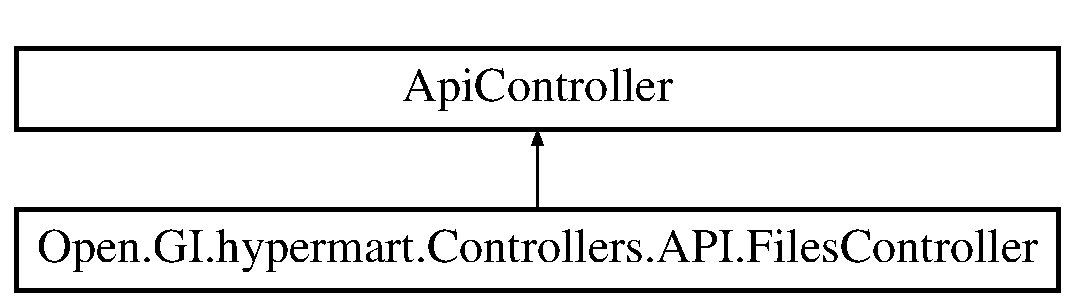
\includegraphics[height=2.000000cm]{class_open_1_1_g_i_1_1hypermart_1_1_controllers_1_1_a_p_i_1_1_files_controller}
\end{center}
\end{figure}
\subsection*{Public Member Functions}
\begin{DoxyCompactItemize}
\item 
I\+Queryable$<$ \textbf{ File} $>$ \textbf{ Get\+Files} ()
\begin{DoxyCompactList}\small\item\em Gets the files. \end{DoxyCompactList}\item 
I\+Http\+Action\+Result \textbf{ Get\+File} (int id)
\begin{DoxyCompactList}\small\item\em Gets the file. \end{DoxyCompactList}\item 
I\+Http\+Action\+Result \textbf{ Put\+File} (int id, \textbf{ File} file)
\begin{DoxyCompactList}\small\item\em Puts the file. \end{DoxyCompactList}\item 
I\+Http\+Action\+Result \textbf{ Post\+File} (\textbf{ File} file)
\begin{DoxyCompactList}\small\item\em Posts the file. \end{DoxyCompactList}\item 
I\+Http\+Action\+Result \textbf{ Delete\+File} (int id)
\begin{DoxyCompactList}\small\item\em Deletes the file. \end{DoxyCompactList}\end{DoxyCompactItemize}
\subsection*{Protected Member Functions}
\begin{DoxyCompactItemize}
\item 
override void \textbf{ Dispose} (bool disposing)
\begin{DoxyCompactList}\small\item\em Releases the unmanaged resources that are used by the object and, optionally, releases the managed resources. \end{DoxyCompactList}\end{DoxyCompactItemize}


\subsection{Detailed Description}
R\+E\+ST \doxyref{A\+PI}{p.}{namespace_open_1_1_g_i_1_1hypermart_1_1_controllers_1_1_a_p_i} layer for interacting with files. 

\begin{DoxySeeAlso}{See also}
System.\+Web.\+Http.\+Api\+Controller


\end{DoxySeeAlso}


Definition at line 20 of file Files\+Controller.\+cs.



\subsection{Member Function Documentation}
\mbox{\label{class_open_1_1_g_i_1_1hypermart_1_1_controllers_1_1_a_p_i_1_1_files_controller_a0eb8a707a270627264d4c2600e8d7671}} 
\index{Open\+::\+G\+I\+::hypermart\+::\+Controllers\+::\+A\+P\+I\+::\+Files\+Controller@{Open\+::\+G\+I\+::hypermart\+::\+Controllers\+::\+A\+P\+I\+::\+Files\+Controller}!Delete\+File@{Delete\+File}}
\index{Delete\+File@{Delete\+File}!Open\+::\+G\+I\+::hypermart\+::\+Controllers\+::\+A\+P\+I\+::\+Files\+Controller@{Open\+::\+G\+I\+::hypermart\+::\+Controllers\+::\+A\+P\+I\+::\+Files\+Controller}}
\subsubsection{Delete\+File()}
{\footnotesize\ttfamily I\+Http\+Action\+Result Open.\+G\+I.\+hypermart.\+Controllers.\+A\+P\+I.\+Files\+Controller.\+Delete\+File (\begin{DoxyParamCaption}\item[{int}]{id }\end{DoxyParamCaption})}



Deletes the file. 


\begin{DoxyParams}{Parameters}
{\em id} & The identifier.\\
\hline
\end{DoxyParams}
\begin{DoxyReturn}{Returns}

\end{DoxyReturn}


Definition at line 120 of file Files\+Controller.\+cs.

\mbox{\label{class_open_1_1_g_i_1_1hypermart_1_1_controllers_1_1_a_p_i_1_1_files_controller_abdd2147a5540d600382f2d1021a6c623}} 
\index{Open\+::\+G\+I\+::hypermart\+::\+Controllers\+::\+A\+P\+I\+::\+Files\+Controller@{Open\+::\+G\+I\+::hypermart\+::\+Controllers\+::\+A\+P\+I\+::\+Files\+Controller}!Dispose@{Dispose}}
\index{Dispose@{Dispose}!Open\+::\+G\+I\+::hypermart\+::\+Controllers\+::\+A\+P\+I\+::\+Files\+Controller@{Open\+::\+G\+I\+::hypermart\+::\+Controllers\+::\+A\+P\+I\+::\+Files\+Controller}}
\subsubsection{Dispose()}
{\footnotesize\ttfamily override void Open.\+G\+I.\+hypermart.\+Controllers.\+A\+P\+I.\+Files\+Controller.\+Dispose (\begin{DoxyParamCaption}\item[{bool}]{disposing }\end{DoxyParamCaption})\hspace{0.3cm}{\ttfamily [protected]}}



Releases the unmanaged resources that are used by the object and, optionally, releases the managed resources. 


\begin{DoxyParams}{Parameters}
{\em disposing} & true to release both managed and unmanaged resources; false to release only unmanaged resources.\\
\hline
\end{DoxyParams}


Definition at line 137 of file Files\+Controller.\+cs.

\mbox{\label{class_open_1_1_g_i_1_1hypermart_1_1_controllers_1_1_a_p_i_1_1_files_controller_ae232956a5cf1b0d749bb27e96154dfd3}} 
\index{Open\+::\+G\+I\+::hypermart\+::\+Controllers\+::\+A\+P\+I\+::\+Files\+Controller@{Open\+::\+G\+I\+::hypermart\+::\+Controllers\+::\+A\+P\+I\+::\+Files\+Controller}!Get\+File@{Get\+File}}
\index{Get\+File@{Get\+File}!Open\+::\+G\+I\+::hypermart\+::\+Controllers\+::\+A\+P\+I\+::\+Files\+Controller@{Open\+::\+G\+I\+::hypermart\+::\+Controllers\+::\+A\+P\+I\+::\+Files\+Controller}}
\subsubsection{Get\+File()}
{\footnotesize\ttfamily I\+Http\+Action\+Result Open.\+G\+I.\+hypermart.\+Controllers.\+A\+P\+I.\+Files\+Controller.\+Get\+File (\begin{DoxyParamCaption}\item[{int}]{id }\end{DoxyParamCaption})}



Gets the file. 


\begin{DoxyParams}{Parameters}
{\em id} & The identifier.\\
\hline
\end{DoxyParams}
\begin{DoxyReturn}{Returns}

\end{DoxyReturn}


Definition at line 41 of file Files\+Controller.\+cs.

\mbox{\label{class_open_1_1_g_i_1_1hypermart_1_1_controllers_1_1_a_p_i_1_1_files_controller_ab9860e1f780182dd01086d07e8bbab65}} 
\index{Open\+::\+G\+I\+::hypermart\+::\+Controllers\+::\+A\+P\+I\+::\+Files\+Controller@{Open\+::\+G\+I\+::hypermart\+::\+Controllers\+::\+A\+P\+I\+::\+Files\+Controller}!Get\+Files@{Get\+Files}}
\index{Get\+Files@{Get\+Files}!Open\+::\+G\+I\+::hypermart\+::\+Controllers\+::\+A\+P\+I\+::\+Files\+Controller@{Open\+::\+G\+I\+::hypermart\+::\+Controllers\+::\+A\+P\+I\+::\+Files\+Controller}}
\subsubsection{Get\+Files()}
{\footnotesize\ttfamily I\+Queryable$<$\textbf{ File}$>$ Open.\+G\+I.\+hypermart.\+Controllers.\+A\+P\+I.\+Files\+Controller.\+Get\+Files (\begin{DoxyParamCaption}{ }\end{DoxyParamCaption})}



Gets the files. 

\begin{DoxyReturn}{Returns}

\end{DoxyReturn}


Definition at line 29 of file Files\+Controller.\+cs.

\mbox{\label{class_open_1_1_g_i_1_1hypermart_1_1_controllers_1_1_a_p_i_1_1_files_controller_a4c176da21d23430d23010248e644d61b}} 
\index{Open\+::\+G\+I\+::hypermart\+::\+Controllers\+::\+A\+P\+I\+::\+Files\+Controller@{Open\+::\+G\+I\+::hypermart\+::\+Controllers\+::\+A\+P\+I\+::\+Files\+Controller}!Post\+File@{Post\+File}}
\index{Post\+File@{Post\+File}!Open\+::\+G\+I\+::hypermart\+::\+Controllers\+::\+A\+P\+I\+::\+Files\+Controller@{Open\+::\+G\+I\+::hypermart\+::\+Controllers\+::\+A\+P\+I\+::\+Files\+Controller}}
\subsubsection{Post\+File()}
{\footnotesize\ttfamily I\+Http\+Action\+Result Open.\+G\+I.\+hypermart.\+Controllers.\+A\+P\+I.\+Files\+Controller.\+Post\+File (\begin{DoxyParamCaption}\item[{\textbf{ File}}]{file }\end{DoxyParamCaption})}



Posts the file. 


\begin{DoxyParams}{Parameters}
{\em file} & The file.\\
\hline
\end{DoxyParams}
\begin{DoxyReturn}{Returns}

\end{DoxyReturn}


Definition at line 100 of file Files\+Controller.\+cs.

\mbox{\label{class_open_1_1_g_i_1_1hypermart_1_1_controllers_1_1_a_p_i_1_1_files_controller_a773d8f70de8b006795b74c1bd921bdb2}} 
\index{Open\+::\+G\+I\+::hypermart\+::\+Controllers\+::\+A\+P\+I\+::\+Files\+Controller@{Open\+::\+G\+I\+::hypermart\+::\+Controllers\+::\+A\+P\+I\+::\+Files\+Controller}!Put\+File@{Put\+File}}
\index{Put\+File@{Put\+File}!Open\+::\+G\+I\+::hypermart\+::\+Controllers\+::\+A\+P\+I\+::\+Files\+Controller@{Open\+::\+G\+I\+::hypermart\+::\+Controllers\+::\+A\+P\+I\+::\+Files\+Controller}}
\subsubsection{Put\+File()}
{\footnotesize\ttfamily I\+Http\+Action\+Result Open.\+G\+I.\+hypermart.\+Controllers.\+A\+P\+I.\+Files\+Controller.\+Put\+File (\begin{DoxyParamCaption}\item[{int}]{id,  }\item[{\textbf{ File}}]{file }\end{DoxyParamCaption})}



Puts the file. 


\begin{DoxyParams}{Parameters}
{\em id} & The identifier.\\
\hline
{\em file} & The file.\\
\hline
\end{DoxyParams}
\begin{DoxyReturn}{Returns}

\end{DoxyReturn}


Definition at line 60 of file Files\+Controller.\+cs.



The documentation for this class was generated from the following file\+:\begin{DoxyCompactItemize}
\item 
C\+:/\+Projects/\+App-\/\+Utility-\/\+Store/\+Open.\+G\+I.\+hypermart/\+Controllers/\+A\+P\+I/\textbf{ Files\+Controller.\+cs}\end{DoxyCompactItemize}

\hypertarget{class_open_1_1_g_i_1_1hypermart_1_1_helpers_1_1_file_share_helper}{}\section{Open.\+G\+I.\+hypermart.\+Helpers.\+File\+Share\+Helper Class Reference}
\label{class_open_1_1_g_i_1_1hypermart_1_1_helpers_1_1_file_share_helper}\index{Open.\+G\+I.\+hypermart.\+Helpers.\+File\+Share\+Helper@{Open.\+G\+I.\+hypermart.\+Helpers.\+File\+Share\+Helper}}


 


\subsection*{Static Public Member Functions}
\begin{DoxyCompactItemize}
\item 
static void \hyperlink{class_open_1_1_g_i_1_1hypermart_1_1_helpers_1_1_file_share_helper_a8e938d7ae2d931ab892c0ebf964ee4d2}{Create\+Folder} (String Folder\+Name)
\begin{DoxyCompactList}\small\item\em Create a Folder -\/ used to create a file System for storing products \end{DoxyCompactList}\item 
static void \hyperlink{class_open_1_1_g_i_1_1hypermart_1_1_helpers_1_1_file_share_helper_af08f7c0abe722a41623b0ae56f78a927}{Create\+Share} (string Folder\+Name, string Share\+Name, string Description)
\begin{DoxyCompactList}\small\item\em Creates the share. \end{DoxyCompactList}\item 
static void \hyperlink{class_open_1_1_g_i_1_1hypermart_1_1_helpers_1_1_file_share_helper_afa333f49f2689e9a64708c27450582ef}{Delete\+Share} (string Folder\+Name)
\begin{DoxyCompactList}\small\item\em Deletes the share. \end{DoxyCompactList}\end{DoxyCompactItemize}


\subsection{Detailed Description}




\subsection{Member Function Documentation}
\hypertarget{class_open_1_1_g_i_1_1hypermart_1_1_helpers_1_1_file_share_helper_a8e938d7ae2d931ab892c0ebf964ee4d2}{}\label{class_open_1_1_g_i_1_1hypermart_1_1_helpers_1_1_file_share_helper_a8e938d7ae2d931ab892c0ebf964ee4d2} 
\index{Open\+::\+G\+I\+::hypermart\+::\+Helpers\+::\+File\+Share\+Helper@{Open\+::\+G\+I\+::hypermart\+::\+Helpers\+::\+File\+Share\+Helper}!Create\+Folder@{Create\+Folder}}
\index{Create\+Folder@{Create\+Folder}!Open\+::\+G\+I\+::hypermart\+::\+Helpers\+::\+File\+Share\+Helper@{Open\+::\+G\+I\+::hypermart\+::\+Helpers\+::\+File\+Share\+Helper}}
\subsubsection{\texorpdfstring{Create\+Folder()}{CreateFolder()}}
{\footnotesize\ttfamily static void Open.\+G\+I.\+hypermart.\+Helpers.\+File\+Share\+Helper.\+Create\+Folder (\begin{DoxyParamCaption}\item[{String}]{Folder\+Name }\end{DoxyParamCaption})\hspace{0.3cm}{\ttfamily [static]}}



Create a Folder -\/ used to create a file System for storing products 


\begin{DoxyParams}{Parameters}
{\em Folder\+Name} & \\
\hline
\end{DoxyParams}
\hypertarget{class_open_1_1_g_i_1_1hypermart_1_1_helpers_1_1_file_share_helper_af08f7c0abe722a41623b0ae56f78a927}{}\label{class_open_1_1_g_i_1_1hypermart_1_1_helpers_1_1_file_share_helper_af08f7c0abe722a41623b0ae56f78a927} 
\index{Open\+::\+G\+I\+::hypermart\+::\+Helpers\+::\+File\+Share\+Helper@{Open\+::\+G\+I\+::hypermart\+::\+Helpers\+::\+File\+Share\+Helper}!Create\+Share@{Create\+Share}}
\index{Create\+Share@{Create\+Share}!Open\+::\+G\+I\+::hypermart\+::\+Helpers\+::\+File\+Share\+Helper@{Open\+::\+G\+I\+::hypermart\+::\+Helpers\+::\+File\+Share\+Helper}}
\subsubsection{\texorpdfstring{Create\+Share()}{CreateShare()}}
{\footnotesize\ttfamily static void Open.\+G\+I.\+hypermart.\+Helpers.\+File\+Share\+Helper.\+Create\+Share (\begin{DoxyParamCaption}\item[{string}]{Folder\+Name,  }\item[{string}]{Share\+Name,  }\item[{string}]{Description }\end{DoxyParamCaption})\hspace{0.3cm}{\ttfamily [static]}}



Creates the share. 


\begin{DoxyParams}{Parameters}
{\em Folder\+Name} & Name of the folder.\\
\hline
{\em Share\+Name} & Name of the share.\\
\hline
{\em Description} & The description.\\
\hline
\end{DoxyParams}

\begin{DoxyExceptions}{Exceptions}
{\em System.\+Exception} & Unable to share directory.\\
\hline
\end{DoxyExceptions}
\hypertarget{class_open_1_1_g_i_1_1hypermart_1_1_helpers_1_1_file_share_helper_afa333f49f2689e9a64708c27450582ef}{}\label{class_open_1_1_g_i_1_1hypermart_1_1_helpers_1_1_file_share_helper_afa333f49f2689e9a64708c27450582ef} 
\index{Open\+::\+G\+I\+::hypermart\+::\+Helpers\+::\+File\+Share\+Helper@{Open\+::\+G\+I\+::hypermart\+::\+Helpers\+::\+File\+Share\+Helper}!Delete\+Share@{Delete\+Share}}
\index{Delete\+Share@{Delete\+Share}!Open\+::\+G\+I\+::hypermart\+::\+Helpers\+::\+File\+Share\+Helper@{Open\+::\+G\+I\+::hypermart\+::\+Helpers\+::\+File\+Share\+Helper}}
\subsubsection{\texorpdfstring{Delete\+Share()}{DeleteShare()}}
{\footnotesize\ttfamily static void Open.\+G\+I.\+hypermart.\+Helpers.\+File\+Share\+Helper.\+Delete\+Share (\begin{DoxyParamCaption}\item[{string}]{Folder\+Name }\end{DoxyParamCaption})\hspace{0.3cm}{\ttfamily [static]}}



Deletes the share. 


\begin{DoxyParams}{Parameters}
{\em Folder\+Name} & Name of the folder.\\
\hline
\end{DoxyParams}


The documentation for this class was generated from the following file\+:\begin{DoxyCompactItemize}
\item 
C\+:/\+Projects/\+App-\/\+Utility-\/\+Store/\+Open.\+G\+I.\+hypermart/\+Helpers/\hyperlink{_file_share_helper_8cs}{File\+Share\+Helper.\+cs}\end{DoxyCompactItemize}

\section{Open.\+G\+I.\+hypermart.\+Filter\+Config Class Reference}
\label{class_open_1_1_g_i_1_1hypermart_1_1_filter_config}\index{Open.\+G\+I.\+hypermart.\+Filter\+Config@{Open.\+G\+I.\+hypermart.\+Filter\+Config}}


Class for filter configuration  


\subsection*{Static Public Member Functions}
\begin{DoxyCompactItemize}
\item 
static void \textbf{ Register\+Global\+Filters} (Global\+Filter\+Collection filters)
\begin{DoxyCompactList}\small\item\em Registers the global filters. \end{DoxyCompactList}\end{DoxyCompactItemize}


\subsection{Detailed Description}
Class for filter configuration 



Definition at line 9 of file Filter\+Config.\+cs.



\subsection{Member Function Documentation}
\mbox{\label{class_open_1_1_g_i_1_1hypermart_1_1_filter_config_a7c2f9e6d0e8157c2942a400ccff8134b}} 
\index{Open\+::\+G\+I\+::hypermart\+::\+Filter\+Config@{Open\+::\+G\+I\+::hypermart\+::\+Filter\+Config}!Register\+Global\+Filters@{Register\+Global\+Filters}}
\index{Register\+Global\+Filters@{Register\+Global\+Filters}!Open\+::\+G\+I\+::hypermart\+::\+Filter\+Config@{Open\+::\+G\+I\+::hypermart\+::\+Filter\+Config}}
\subsubsection{Register\+Global\+Filters()}
{\footnotesize\ttfamily static void Open.\+G\+I.\+hypermart.\+Filter\+Config.\+Register\+Global\+Filters (\begin{DoxyParamCaption}\item[{Global\+Filter\+Collection}]{filters }\end{DoxyParamCaption})\hspace{0.3cm}{\ttfamily [static]}}



Registers the global filters. 


\begin{DoxyParams}{Parameters}
{\em filters} & The filters.\\
\hline
\end{DoxyParams}


Definition at line 15 of file Filter\+Config.\+cs.



The documentation for this class was generated from the following file\+:\begin{DoxyCompactItemize}
\item 
C\+:/\+Projects/\+App-\/\+Utility-\/\+Store/\+Open.\+G\+I.\+hypermart/\+App\+\_\+\+Start/\textbf{ Filter\+Config.\+cs}\end{DoxyCompactItemize}

\section{Open.\+G\+I.\+hypermart.\+Areas.\+Help\+Page.\+Controllers.\+Help\+Controller Class Reference}
\label{class_open_1_1_g_i_1_1hypermart_1_1_areas_1_1_help_page_1_1_controllers_1_1_help_controller}\index{Open.\+G\+I.\+hypermart.\+Areas.\+Help\+Page.\+Controllers.\+Help\+Controller@{Open.\+G\+I.\+hypermart.\+Areas.\+Help\+Page.\+Controllers.\+Help\+Controller}}


The controller that will handle requests for the help page.  


Inheritance diagram for Open.\+G\+I.\+hypermart.\+Areas.\+Help\+Page.\+Controllers.\+Help\+Controller\+:\begin{figure}[H]
\begin{center}
\leavevmode
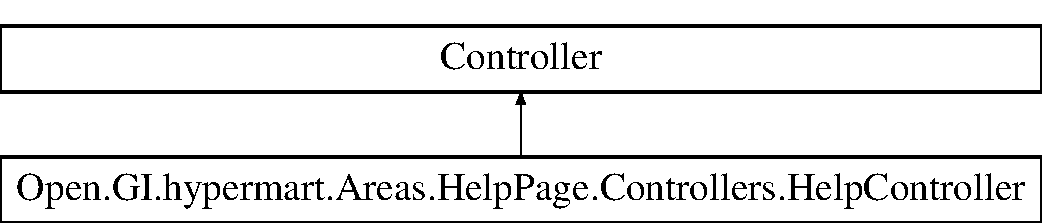
\includegraphics[height=2.000000cm]{class_open_1_1_g_i_1_1hypermart_1_1_areas_1_1_help_page_1_1_controllers_1_1_help_controller}
\end{center}
\end{figure}
\subsection*{Public Member Functions}
\begin{DoxyCompactItemize}
\item 
\textbf{ Help\+Controller} ()
\begin{DoxyCompactList}\small\item\em Initializes a new instance of the \doxyref{Help\+Controller}{p.}{class_open_1_1_g_i_1_1hypermart_1_1_areas_1_1_help_page_1_1_controllers_1_1_help_controller} class. \end{DoxyCompactList}\item 
\textbf{ Help\+Controller} (Http\+Configuration config)
\begin{DoxyCompactList}\small\item\em Initializes a new instance of the \doxyref{Help\+Controller}{p.}{class_open_1_1_g_i_1_1hypermart_1_1_areas_1_1_help_page_1_1_controllers_1_1_help_controller} class. \end{DoxyCompactList}\item 
Action\+Result \textbf{ Index} ()
\begin{DoxyCompactList}\small\item\em Indexes this instance. \end{DoxyCompactList}\item 
Action\+Result \textbf{ Api} (string api\+Id)
\begin{DoxyCompactList}\small\item\em A\+P\+Is the specified A\+PI identifier. \end{DoxyCompactList}\item 
Action\+Result \textbf{ Resource\+Model} (string model\+Name)
\begin{DoxyCompactList}\small\item\em Resources the model. \end{DoxyCompactList}\end{DoxyCompactItemize}
\subsection*{Properties}
\begin{DoxyCompactItemize}
\item 
Http\+Configuration \textbf{ Configuration}\hspace{0.3cm}{\ttfamily  [get]}
\begin{DoxyCompactList}\small\item\em Gets the configuration. \end{DoxyCompactList}\end{DoxyCompactItemize}


\subsection{Detailed Description}
The controller that will handle requests for the help page. 



Definition at line 12 of file Help\+Controller.\+cs.



\subsection{Constructor \& Destructor Documentation}
\mbox{\label{class_open_1_1_g_i_1_1hypermart_1_1_areas_1_1_help_page_1_1_controllers_1_1_help_controller_afa0b9b820c64c6b4f58818ea7a8fbee9}} 
\index{Open\+::\+G\+I\+::hypermart\+::\+Areas\+::\+Help\+Page\+::\+Controllers\+::\+Help\+Controller@{Open\+::\+G\+I\+::hypermart\+::\+Areas\+::\+Help\+Page\+::\+Controllers\+::\+Help\+Controller}!Help\+Controller@{Help\+Controller}}
\index{Help\+Controller@{Help\+Controller}!Open\+::\+G\+I\+::hypermart\+::\+Areas\+::\+Help\+Page\+::\+Controllers\+::\+Help\+Controller@{Open\+::\+G\+I\+::hypermart\+::\+Areas\+::\+Help\+Page\+::\+Controllers\+::\+Help\+Controller}}
\subsubsection{Help\+Controller()\hspace{0.1cm}{\footnotesize\ttfamily [1/2]}}
{\footnotesize\ttfamily Open.\+G\+I.\+hypermart.\+Areas.\+Help\+Page.\+Controllers.\+Help\+Controller.\+Help\+Controller (\begin{DoxyParamCaption}{ }\end{DoxyParamCaption})}



Initializes a new instance of the \doxyref{Help\+Controller}{p.}{class_open_1_1_g_i_1_1hypermart_1_1_areas_1_1_help_page_1_1_controllers_1_1_help_controller} class. 



Definition at line 19 of file Help\+Controller.\+cs.

\mbox{\label{class_open_1_1_g_i_1_1hypermart_1_1_areas_1_1_help_page_1_1_controllers_1_1_help_controller_a5701fb0613147c92bcf47b40636fbb4c}} 
\index{Open\+::\+G\+I\+::hypermart\+::\+Areas\+::\+Help\+Page\+::\+Controllers\+::\+Help\+Controller@{Open\+::\+G\+I\+::hypermart\+::\+Areas\+::\+Help\+Page\+::\+Controllers\+::\+Help\+Controller}!Help\+Controller@{Help\+Controller}}
\index{Help\+Controller@{Help\+Controller}!Open\+::\+G\+I\+::hypermart\+::\+Areas\+::\+Help\+Page\+::\+Controllers\+::\+Help\+Controller@{Open\+::\+G\+I\+::hypermart\+::\+Areas\+::\+Help\+Page\+::\+Controllers\+::\+Help\+Controller}}
\subsubsection{Help\+Controller()\hspace{0.1cm}{\footnotesize\ttfamily [2/2]}}
{\footnotesize\ttfamily Open.\+G\+I.\+hypermart.\+Areas.\+Help\+Page.\+Controllers.\+Help\+Controller.\+Help\+Controller (\begin{DoxyParamCaption}\item[{Http\+Configuration}]{config }\end{DoxyParamCaption})}



Initializes a new instance of the \doxyref{Help\+Controller}{p.}{class_open_1_1_g_i_1_1hypermart_1_1_areas_1_1_help_page_1_1_controllers_1_1_help_controller} class. 


\begin{DoxyParams}{Parameters}
{\em config} & The configuration.\\
\hline
\end{DoxyParams}


Definition at line 28 of file Help\+Controller.\+cs.



\subsection{Member Function Documentation}
\mbox{\label{class_open_1_1_g_i_1_1hypermart_1_1_areas_1_1_help_page_1_1_controllers_1_1_help_controller_a5f4e23a5d390343976a5b04f7a3e9344}} 
\index{Open\+::\+G\+I\+::hypermart\+::\+Areas\+::\+Help\+Page\+::\+Controllers\+::\+Help\+Controller@{Open\+::\+G\+I\+::hypermart\+::\+Areas\+::\+Help\+Page\+::\+Controllers\+::\+Help\+Controller}!Api@{Api}}
\index{Api@{Api}!Open\+::\+G\+I\+::hypermart\+::\+Areas\+::\+Help\+Page\+::\+Controllers\+::\+Help\+Controller@{Open\+::\+G\+I\+::hypermart\+::\+Areas\+::\+Help\+Page\+::\+Controllers\+::\+Help\+Controller}}
\subsubsection{Api()}
{\footnotesize\ttfamily Action\+Result Open.\+G\+I.\+hypermart.\+Areas.\+Help\+Page.\+Controllers.\+Help\+Controller.\+Api (\begin{DoxyParamCaption}\item[{string}]{api\+Id }\end{DoxyParamCaption})}



A\+P\+Is the specified A\+PI identifier. 


\begin{DoxyParams}{Parameters}
{\em api\+Id} & The A\+PI identifier.\\
\hline
\end{DoxyParams}
\begin{DoxyReturn}{Returns}

\end{DoxyReturn}


Definition at line 56 of file Help\+Controller.\+cs.

\mbox{\label{class_open_1_1_g_i_1_1hypermart_1_1_areas_1_1_help_page_1_1_controllers_1_1_help_controller_a4c63414e59364e8ce99be20a5c909da8}} 
\index{Open\+::\+G\+I\+::hypermart\+::\+Areas\+::\+Help\+Page\+::\+Controllers\+::\+Help\+Controller@{Open\+::\+G\+I\+::hypermart\+::\+Areas\+::\+Help\+Page\+::\+Controllers\+::\+Help\+Controller}!Index@{Index}}
\index{Index@{Index}!Open\+::\+G\+I\+::hypermart\+::\+Areas\+::\+Help\+Page\+::\+Controllers\+::\+Help\+Controller@{Open\+::\+G\+I\+::hypermart\+::\+Areas\+::\+Help\+Page\+::\+Controllers\+::\+Help\+Controller}}
\subsubsection{Index()}
{\footnotesize\ttfamily Action\+Result Open.\+G\+I.\+hypermart.\+Areas.\+Help\+Page.\+Controllers.\+Help\+Controller.\+Index (\begin{DoxyParamCaption}{ }\end{DoxyParamCaption})}



Indexes this instance. 

\begin{DoxyReturn}{Returns}

\end{DoxyReturn}


Definition at line 45 of file Help\+Controller.\+cs.

\mbox{\label{class_open_1_1_g_i_1_1hypermart_1_1_areas_1_1_help_page_1_1_controllers_1_1_help_controller_a374c9c2d8d4630c433a397b3ac76c53c}} 
\index{Open\+::\+G\+I\+::hypermart\+::\+Areas\+::\+Help\+Page\+::\+Controllers\+::\+Help\+Controller@{Open\+::\+G\+I\+::hypermart\+::\+Areas\+::\+Help\+Page\+::\+Controllers\+::\+Help\+Controller}!Resource\+Model@{Resource\+Model}}
\index{Resource\+Model@{Resource\+Model}!Open\+::\+G\+I\+::hypermart\+::\+Areas\+::\+Help\+Page\+::\+Controllers\+::\+Help\+Controller@{Open\+::\+G\+I\+::hypermart\+::\+Areas\+::\+Help\+Page\+::\+Controllers\+::\+Help\+Controller}}
\subsubsection{Resource\+Model()}
{\footnotesize\ttfamily Action\+Result Open.\+G\+I.\+hypermart.\+Areas.\+Help\+Page.\+Controllers.\+Help\+Controller.\+Resource\+Model (\begin{DoxyParamCaption}\item[{string}]{model\+Name }\end{DoxyParamCaption})}



Resources the model. 


\begin{DoxyParams}{Parameters}
{\em model\+Name} & Name of the model.\\
\hline
\end{DoxyParams}
\begin{DoxyReturn}{Returns}

\end{DoxyReturn}


Definition at line 75 of file Help\+Controller.\+cs.



\subsection{Property Documentation}
\mbox{\label{class_open_1_1_g_i_1_1hypermart_1_1_areas_1_1_help_page_1_1_controllers_1_1_help_controller_ac1327fb5827701100fa4e1b3566fd752}} 
\index{Open\+::\+G\+I\+::hypermart\+::\+Areas\+::\+Help\+Page\+::\+Controllers\+::\+Help\+Controller@{Open\+::\+G\+I\+::hypermart\+::\+Areas\+::\+Help\+Page\+::\+Controllers\+::\+Help\+Controller}!Configuration@{Configuration}}
\index{Configuration@{Configuration}!Open\+::\+G\+I\+::hypermart\+::\+Areas\+::\+Help\+Page\+::\+Controllers\+::\+Help\+Controller@{Open\+::\+G\+I\+::hypermart\+::\+Areas\+::\+Help\+Page\+::\+Controllers\+::\+Help\+Controller}}
\subsubsection{Configuration}
{\footnotesize\ttfamily Http\+Configuration Open.\+G\+I.\+hypermart.\+Areas.\+Help\+Page.\+Controllers.\+Help\+Controller.\+Configuration\hspace{0.3cm}{\ttfamily [get]}}



Gets the configuration. 

The configuration. 

Definition at line 39 of file Help\+Controller.\+cs.



The documentation for this class was generated from the following file\+:\begin{DoxyCompactItemize}
\item 
C\+:/\+Projects/\+App-\/\+Utility-\/\+Store/\+Open.\+G\+I.\+hypermart/\+Areas/\+Help\+Page/\+Controllers/\textbf{ Help\+Controller.\+cs}\end{DoxyCompactItemize}

\section{Open.\+G\+I.\+hypermart.\+Areas.\+Help\+Page.\+Models.\+Help\+Page\+Api\+Model Class Reference}
\label{class_open_1_1_g_i_1_1hypermart_1_1_areas_1_1_help_page_1_1_models_1_1_help_page_api_model}\index{Open.\+G\+I.\+hypermart.\+Areas.\+Help\+Page.\+Models.\+Help\+Page\+Api\+Model@{Open.\+G\+I.\+hypermart.\+Areas.\+Help\+Page.\+Models.\+Help\+Page\+Api\+Model}}


The model that represents an A\+PI displayed on the help page.  


\subsection*{Public Member Functions}
\begin{DoxyCompactItemize}
\item 
\textbf{ Help\+Page\+Api\+Model} ()
\begin{DoxyCompactList}\small\item\em Initializes a new instance of the \doxyref{Help\+Page\+Api\+Model}{p.}{class_open_1_1_g_i_1_1hypermart_1_1_areas_1_1_help_page_1_1_models_1_1_help_page_api_model} class. \end{DoxyCompactList}\end{DoxyCompactItemize}
\subsection*{Properties}
\begin{DoxyCompactItemize}
\item 
Api\+Description \textbf{ Api\+Description}\hspace{0.3cm}{\ttfamily  [get, set]}
\begin{DoxyCompactList}\small\item\em Gets or sets the \doxyref{Api\+Description}{p.}{class_open_1_1_g_i_1_1hypermart_1_1_areas_1_1_help_page_1_1_models_1_1_help_page_api_model_a80061bc5f25f38dbfbff06705a48372e} that describes the A\+PI. \end{DoxyCompactList}\item 
Collection$<$ \textbf{ Parameter\+Description} $>$ \textbf{ Uri\+Parameters}\hspace{0.3cm}{\ttfamily  [get]}
\begin{DoxyCompactList}\small\item\em Gets or sets the Parameter\+Description collection that describes the U\+RI parameters for the A\+PI. \end{DoxyCompactList}\item 
string \textbf{ Request\+Documentation}\hspace{0.3cm}{\ttfamily  [get, set]}
\begin{DoxyCompactList}\small\item\em Gets or sets the documentation for the request. \end{DoxyCompactList}\item 
\textbf{ Model\+Description} \textbf{ Request\+Model\+Description}\hspace{0.3cm}{\ttfamily  [get, set]}
\begin{DoxyCompactList}\small\item\em Gets or sets the Model\+Description that describes the request body. \end{DoxyCompactList}\item 
I\+List$<$ \textbf{ Parameter\+Description} $>$ \textbf{ Request\+Body\+Parameters}\hspace{0.3cm}{\ttfamily  [get]}
\begin{DoxyCompactList}\small\item\em Gets the request body parameter descriptions. \end{DoxyCompactList}\item 
\textbf{ Model\+Description} \textbf{ Resource\+Description}\hspace{0.3cm}{\ttfamily  [get, set]}
\begin{DoxyCompactList}\small\item\em Gets or sets the Model\+Description that describes the resource. \end{DoxyCompactList}\item 
I\+List$<$ \textbf{ Parameter\+Description} $>$ \textbf{ Resource\+Properties}\hspace{0.3cm}{\ttfamily  [get]}
\begin{DoxyCompactList}\small\item\em Gets the resource property descriptions. \end{DoxyCompactList}\item 
I\+Dictionary$<$ Media\+Type\+Header\+Value, object $>$ \textbf{ Sample\+Requests}\hspace{0.3cm}{\ttfamily  [get]}
\begin{DoxyCompactList}\small\item\em Gets the sample requests associated with the A\+PI. \end{DoxyCompactList}\item 
I\+Dictionary$<$ Media\+Type\+Header\+Value, object $>$ \textbf{ Sample\+Responses}\hspace{0.3cm}{\ttfamily  [get]}
\begin{DoxyCompactList}\small\item\em Gets the sample responses associated with the A\+PI. \end{DoxyCompactList}\item 
Collection$<$ string $>$ \textbf{ Error\+Messages}\hspace{0.3cm}{\ttfamily  [get]}
\begin{DoxyCompactList}\small\item\em Gets the error messages associated with this model. \end{DoxyCompactList}\end{DoxyCompactItemize}


\subsection{Detailed Description}
The model that represents an A\+PI displayed on the help page. 



Definition at line 12 of file Help\+Page\+Api\+Model.\+cs.



\subsection{Constructor \& Destructor Documentation}
\mbox{\label{class_open_1_1_g_i_1_1hypermart_1_1_areas_1_1_help_page_1_1_models_1_1_help_page_api_model_a34aa95dfea87b53bcfac8601fb1f3b93}} 
\index{Open\+::\+G\+I\+::hypermart\+::\+Areas\+::\+Help\+Page\+::\+Models\+::\+Help\+Page\+Api\+Model@{Open\+::\+G\+I\+::hypermart\+::\+Areas\+::\+Help\+Page\+::\+Models\+::\+Help\+Page\+Api\+Model}!Help\+Page\+Api\+Model@{Help\+Page\+Api\+Model}}
\index{Help\+Page\+Api\+Model@{Help\+Page\+Api\+Model}!Open\+::\+G\+I\+::hypermart\+::\+Areas\+::\+Help\+Page\+::\+Models\+::\+Help\+Page\+Api\+Model@{Open\+::\+G\+I\+::hypermart\+::\+Areas\+::\+Help\+Page\+::\+Models\+::\+Help\+Page\+Api\+Model}}
\subsubsection{Help\+Page\+Api\+Model()}
{\footnotesize\ttfamily Open.\+G\+I.\+hypermart.\+Areas.\+Help\+Page.\+Models.\+Help\+Page\+Api\+Model.\+Help\+Page\+Api\+Model (\begin{DoxyParamCaption}{ }\end{DoxyParamCaption})}



Initializes a new instance of the \doxyref{Help\+Page\+Api\+Model}{p.}{class_open_1_1_g_i_1_1hypermart_1_1_areas_1_1_help_page_1_1_models_1_1_help_page_api_model} class. 



Definition at line 17 of file Help\+Page\+Api\+Model.\+cs.



\subsection{Property Documentation}
\mbox{\label{class_open_1_1_g_i_1_1hypermart_1_1_areas_1_1_help_page_1_1_models_1_1_help_page_api_model_a80061bc5f25f38dbfbff06705a48372e}} 
\index{Open\+::\+G\+I\+::hypermart\+::\+Areas\+::\+Help\+Page\+::\+Models\+::\+Help\+Page\+Api\+Model@{Open\+::\+G\+I\+::hypermart\+::\+Areas\+::\+Help\+Page\+::\+Models\+::\+Help\+Page\+Api\+Model}!Api\+Description@{Api\+Description}}
\index{Api\+Description@{Api\+Description}!Open\+::\+G\+I\+::hypermart\+::\+Areas\+::\+Help\+Page\+::\+Models\+::\+Help\+Page\+Api\+Model@{Open\+::\+G\+I\+::hypermart\+::\+Areas\+::\+Help\+Page\+::\+Models\+::\+Help\+Page\+Api\+Model}}
\subsubsection{Api\+Description}
{\footnotesize\ttfamily Api\+Description Open.\+G\+I.\+hypermart.\+Areas.\+Help\+Page.\+Models.\+Help\+Page\+Api\+Model.\+Api\+Description\hspace{0.3cm}{\ttfamily [get]}, {\ttfamily [set]}}



Gets or sets the \doxyref{Api\+Description}{p.}{class_open_1_1_g_i_1_1hypermart_1_1_areas_1_1_help_page_1_1_models_1_1_help_page_api_model_a80061bc5f25f38dbfbff06705a48372e} that describes the A\+PI. 



Definition at line 28 of file Help\+Page\+Api\+Model.\+cs.

\mbox{\label{class_open_1_1_g_i_1_1hypermart_1_1_areas_1_1_help_page_1_1_models_1_1_help_page_api_model_a318df386bf722bfbafab9a6f2812641e}} 
\index{Open\+::\+G\+I\+::hypermart\+::\+Areas\+::\+Help\+Page\+::\+Models\+::\+Help\+Page\+Api\+Model@{Open\+::\+G\+I\+::hypermart\+::\+Areas\+::\+Help\+Page\+::\+Models\+::\+Help\+Page\+Api\+Model}!Error\+Messages@{Error\+Messages}}
\index{Error\+Messages@{Error\+Messages}!Open\+::\+G\+I\+::hypermart\+::\+Areas\+::\+Help\+Page\+::\+Models\+::\+Help\+Page\+Api\+Model@{Open\+::\+G\+I\+::hypermart\+::\+Areas\+::\+Help\+Page\+::\+Models\+::\+Help\+Page\+Api\+Model}}
\subsubsection{Error\+Messages}
{\footnotesize\ttfamily Collection$<$string$>$ Open.\+G\+I.\+hypermart.\+Areas.\+Help\+Page.\+Models.\+Help\+Page\+Api\+Model.\+Error\+Messages\hspace{0.3cm}{\ttfamily [get]}}



Gets the error messages associated with this model. 



Definition at line 85 of file Help\+Page\+Api\+Model.\+cs.

\mbox{\label{class_open_1_1_g_i_1_1hypermart_1_1_areas_1_1_help_page_1_1_models_1_1_help_page_api_model_a6b2ccd725318cec7557237bb25272ac0}} 
\index{Open\+::\+G\+I\+::hypermart\+::\+Areas\+::\+Help\+Page\+::\+Models\+::\+Help\+Page\+Api\+Model@{Open\+::\+G\+I\+::hypermart\+::\+Areas\+::\+Help\+Page\+::\+Models\+::\+Help\+Page\+Api\+Model}!Request\+Body\+Parameters@{Request\+Body\+Parameters}}
\index{Request\+Body\+Parameters@{Request\+Body\+Parameters}!Open\+::\+G\+I\+::hypermart\+::\+Areas\+::\+Help\+Page\+::\+Models\+::\+Help\+Page\+Api\+Model@{Open\+::\+G\+I\+::hypermart\+::\+Areas\+::\+Help\+Page\+::\+Models\+::\+Help\+Page\+Api\+Model}}
\subsubsection{Request\+Body\+Parameters}
{\footnotesize\ttfamily I\+List$<$\textbf{ Parameter\+Description}$>$ Open.\+G\+I.\+hypermart.\+Areas.\+Help\+Page.\+Models.\+Help\+Page\+Api\+Model.\+Request\+Body\+Parameters\hspace{0.3cm}{\ttfamily [get]}}



Gets the request body parameter descriptions. 



Definition at line 49 of file Help\+Page\+Api\+Model.\+cs.

\mbox{\label{class_open_1_1_g_i_1_1hypermart_1_1_areas_1_1_help_page_1_1_models_1_1_help_page_api_model_aa27a2376388763669d59b97fab474a47}} 
\index{Open\+::\+G\+I\+::hypermart\+::\+Areas\+::\+Help\+Page\+::\+Models\+::\+Help\+Page\+Api\+Model@{Open\+::\+G\+I\+::hypermart\+::\+Areas\+::\+Help\+Page\+::\+Models\+::\+Help\+Page\+Api\+Model}!Request\+Documentation@{Request\+Documentation}}
\index{Request\+Documentation@{Request\+Documentation}!Open\+::\+G\+I\+::hypermart\+::\+Areas\+::\+Help\+Page\+::\+Models\+::\+Help\+Page\+Api\+Model@{Open\+::\+G\+I\+::hypermart\+::\+Areas\+::\+Help\+Page\+::\+Models\+::\+Help\+Page\+Api\+Model}}
\subsubsection{Request\+Documentation}
{\footnotesize\ttfamily string Open.\+G\+I.\+hypermart.\+Areas.\+Help\+Page.\+Models.\+Help\+Page\+Api\+Model.\+Request\+Documentation\hspace{0.3cm}{\ttfamily [get]}, {\ttfamily [set]}}



Gets or sets the documentation for the request. 



Definition at line 38 of file Help\+Page\+Api\+Model.\+cs.

\mbox{\label{class_open_1_1_g_i_1_1hypermart_1_1_areas_1_1_help_page_1_1_models_1_1_help_page_api_model_a9922daf50e7226b541b2906b6011947c}} 
\index{Open\+::\+G\+I\+::hypermart\+::\+Areas\+::\+Help\+Page\+::\+Models\+::\+Help\+Page\+Api\+Model@{Open\+::\+G\+I\+::hypermart\+::\+Areas\+::\+Help\+Page\+::\+Models\+::\+Help\+Page\+Api\+Model}!Request\+Model\+Description@{Request\+Model\+Description}}
\index{Request\+Model\+Description@{Request\+Model\+Description}!Open\+::\+G\+I\+::hypermart\+::\+Areas\+::\+Help\+Page\+::\+Models\+::\+Help\+Page\+Api\+Model@{Open\+::\+G\+I\+::hypermart\+::\+Areas\+::\+Help\+Page\+::\+Models\+::\+Help\+Page\+Api\+Model}}
\subsubsection{Request\+Model\+Description}
{\footnotesize\ttfamily \textbf{ Model\+Description} Open.\+G\+I.\+hypermart.\+Areas.\+Help\+Page.\+Models.\+Help\+Page\+Api\+Model.\+Request\+Model\+Description\hspace{0.3cm}{\ttfamily [get]}, {\ttfamily [set]}}



Gets or sets the Model\+Description that describes the request body. 



Definition at line 43 of file Help\+Page\+Api\+Model.\+cs.

\mbox{\label{class_open_1_1_g_i_1_1hypermart_1_1_areas_1_1_help_page_1_1_models_1_1_help_page_api_model_a69f18559e320aecc4dc81f68b8327729}} 
\index{Open\+::\+G\+I\+::hypermart\+::\+Areas\+::\+Help\+Page\+::\+Models\+::\+Help\+Page\+Api\+Model@{Open\+::\+G\+I\+::hypermart\+::\+Areas\+::\+Help\+Page\+::\+Models\+::\+Help\+Page\+Api\+Model}!Resource\+Description@{Resource\+Description}}
\index{Resource\+Description@{Resource\+Description}!Open\+::\+G\+I\+::hypermart\+::\+Areas\+::\+Help\+Page\+::\+Models\+::\+Help\+Page\+Api\+Model@{Open\+::\+G\+I\+::hypermart\+::\+Areas\+::\+Help\+Page\+::\+Models\+::\+Help\+Page\+Api\+Model}}
\subsubsection{Resource\+Description}
{\footnotesize\ttfamily \textbf{ Model\+Description} Open.\+G\+I.\+hypermart.\+Areas.\+Help\+Page.\+Models.\+Help\+Page\+Api\+Model.\+Resource\+Description\hspace{0.3cm}{\ttfamily [get]}, {\ttfamily [set]}}



Gets or sets the Model\+Description that describes the resource. 



Definition at line 59 of file Help\+Page\+Api\+Model.\+cs.

\mbox{\label{class_open_1_1_g_i_1_1hypermart_1_1_areas_1_1_help_page_1_1_models_1_1_help_page_api_model_a1fc678443900b538ee0b4bbd22e9b4d3}} 
\index{Open\+::\+G\+I\+::hypermart\+::\+Areas\+::\+Help\+Page\+::\+Models\+::\+Help\+Page\+Api\+Model@{Open\+::\+G\+I\+::hypermart\+::\+Areas\+::\+Help\+Page\+::\+Models\+::\+Help\+Page\+Api\+Model}!Resource\+Properties@{Resource\+Properties}}
\index{Resource\+Properties@{Resource\+Properties}!Open\+::\+G\+I\+::hypermart\+::\+Areas\+::\+Help\+Page\+::\+Models\+::\+Help\+Page\+Api\+Model@{Open\+::\+G\+I\+::hypermart\+::\+Areas\+::\+Help\+Page\+::\+Models\+::\+Help\+Page\+Api\+Model}}
\subsubsection{Resource\+Properties}
{\footnotesize\ttfamily I\+List$<$\textbf{ Parameter\+Description}$>$ Open.\+G\+I.\+hypermart.\+Areas.\+Help\+Page.\+Models.\+Help\+Page\+Api\+Model.\+Resource\+Properties\hspace{0.3cm}{\ttfamily [get]}}



Gets the resource property descriptions. 



Definition at line 65 of file Help\+Page\+Api\+Model.\+cs.

\mbox{\label{class_open_1_1_g_i_1_1hypermart_1_1_areas_1_1_help_page_1_1_models_1_1_help_page_api_model_a5ba6db9c9586dc77949e8d824cca46b3}} 
\index{Open\+::\+G\+I\+::hypermart\+::\+Areas\+::\+Help\+Page\+::\+Models\+::\+Help\+Page\+Api\+Model@{Open\+::\+G\+I\+::hypermart\+::\+Areas\+::\+Help\+Page\+::\+Models\+::\+Help\+Page\+Api\+Model}!Sample\+Requests@{Sample\+Requests}}
\index{Sample\+Requests@{Sample\+Requests}!Open\+::\+G\+I\+::hypermart\+::\+Areas\+::\+Help\+Page\+::\+Models\+::\+Help\+Page\+Api\+Model@{Open\+::\+G\+I\+::hypermart\+::\+Areas\+::\+Help\+Page\+::\+Models\+::\+Help\+Page\+Api\+Model}}
\subsubsection{Sample\+Requests}
{\footnotesize\ttfamily I\+Dictionary$<$Media\+Type\+Header\+Value, object$>$ Open.\+G\+I.\+hypermart.\+Areas.\+Help\+Page.\+Models.\+Help\+Page\+Api\+Model.\+Sample\+Requests\hspace{0.3cm}{\ttfamily [get]}}



Gets the sample requests associated with the A\+PI. 



Definition at line 75 of file Help\+Page\+Api\+Model.\+cs.

\mbox{\label{class_open_1_1_g_i_1_1hypermart_1_1_areas_1_1_help_page_1_1_models_1_1_help_page_api_model_a08ca3610bd41722c64d0a58231e358a3}} 
\index{Open\+::\+G\+I\+::hypermart\+::\+Areas\+::\+Help\+Page\+::\+Models\+::\+Help\+Page\+Api\+Model@{Open\+::\+G\+I\+::hypermart\+::\+Areas\+::\+Help\+Page\+::\+Models\+::\+Help\+Page\+Api\+Model}!Sample\+Responses@{Sample\+Responses}}
\index{Sample\+Responses@{Sample\+Responses}!Open\+::\+G\+I\+::hypermart\+::\+Areas\+::\+Help\+Page\+::\+Models\+::\+Help\+Page\+Api\+Model@{Open\+::\+G\+I\+::hypermart\+::\+Areas\+::\+Help\+Page\+::\+Models\+::\+Help\+Page\+Api\+Model}}
\subsubsection{Sample\+Responses}
{\footnotesize\ttfamily I\+Dictionary$<$Media\+Type\+Header\+Value, object$>$ Open.\+G\+I.\+hypermart.\+Areas.\+Help\+Page.\+Models.\+Help\+Page\+Api\+Model.\+Sample\+Responses\hspace{0.3cm}{\ttfamily [get]}}



Gets the sample responses associated with the A\+PI. 



Definition at line 80 of file Help\+Page\+Api\+Model.\+cs.

\mbox{\label{class_open_1_1_g_i_1_1hypermart_1_1_areas_1_1_help_page_1_1_models_1_1_help_page_api_model_a1ff7528f7e83c0a9951649f44f55745f}} 
\index{Open\+::\+G\+I\+::hypermart\+::\+Areas\+::\+Help\+Page\+::\+Models\+::\+Help\+Page\+Api\+Model@{Open\+::\+G\+I\+::hypermart\+::\+Areas\+::\+Help\+Page\+::\+Models\+::\+Help\+Page\+Api\+Model}!Uri\+Parameters@{Uri\+Parameters}}
\index{Uri\+Parameters@{Uri\+Parameters}!Open\+::\+G\+I\+::hypermart\+::\+Areas\+::\+Help\+Page\+::\+Models\+::\+Help\+Page\+Api\+Model@{Open\+::\+G\+I\+::hypermart\+::\+Areas\+::\+Help\+Page\+::\+Models\+::\+Help\+Page\+Api\+Model}}
\subsubsection{Uri\+Parameters}
{\footnotesize\ttfamily Collection$<$\textbf{ Parameter\+Description}$>$ Open.\+G\+I.\+hypermart.\+Areas.\+Help\+Page.\+Models.\+Help\+Page\+Api\+Model.\+Uri\+Parameters\hspace{0.3cm}{\ttfamily [get]}}



Gets or sets the Parameter\+Description collection that describes the U\+RI parameters for the A\+PI. 



Definition at line 33 of file Help\+Page\+Api\+Model.\+cs.



The documentation for this class was generated from the following file\+:\begin{DoxyCompactItemize}
\item 
C\+:/\+Projects/\+App-\/\+Utility-\/\+Store/\+Open.\+G\+I.\+hypermart/\+Areas/\+Help\+Page/\+Models/\textbf{ Help\+Page\+Api\+Model.\+cs}\end{DoxyCompactItemize}

\section{Open.\+G\+I.\+hypermart.\+Areas.\+Help\+Page.\+Help\+Page\+Area\+Registration Class Reference}
\label{class_open_1_1_g_i_1_1hypermart_1_1_areas_1_1_help_page_1_1_help_page_area_registration}\index{Open.\+G\+I.\+hypermart.\+Areas.\+Help\+Page.\+Help\+Page\+Area\+Registration@{Open.\+G\+I.\+hypermart.\+Areas.\+Help\+Page.\+Help\+Page\+Area\+Registration}}


 


Inheritance diagram for Open.\+G\+I.\+hypermart.\+Areas.\+Help\+Page.\+Help\+Page\+Area\+Registration\+:\begin{figure}[H]
\begin{center}
\leavevmode
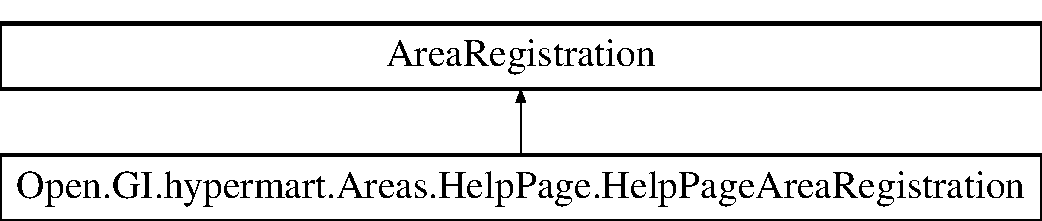
\includegraphics[height=2.000000cm]{class_open_1_1_g_i_1_1hypermart_1_1_areas_1_1_help_page_1_1_help_page_area_registration}
\end{center}
\end{figure}
\subsection*{Public Member Functions}
\begin{DoxyCompactItemize}
\item 
override void \textbf{ Register\+Area} (Area\+Registration\+Context context)
\begin{DoxyCompactList}\small\item\em Registers an area in an A\+S\+P.\+N\+ET M\+VC application using the specified area\textquotesingle{}s context information. \end{DoxyCompactList}\end{DoxyCompactItemize}
\subsection*{Properties}
\begin{DoxyCompactItemize}
\item 
override string \textbf{ Area\+Name}\hspace{0.3cm}{\ttfamily  [get]}
\begin{DoxyCompactList}\small\item\em Gets the name of the area to register. \end{DoxyCompactList}\end{DoxyCompactItemize}


\subsection{Detailed Description}


\begin{DoxySeeAlso}{See also}
System.\+Web.\+Mvc.\+Area\+Registration


\end{DoxySeeAlso}


Definition at line 10 of file Help\+Page\+Area\+Registration.\+cs.



\subsection{Member Function Documentation}
\mbox{\label{class_open_1_1_g_i_1_1hypermart_1_1_areas_1_1_help_page_1_1_help_page_area_registration_aee73751274402f096ce32ee010ef1a11}} 
\index{Open\+::\+G\+I\+::hypermart\+::\+Areas\+::\+Help\+Page\+::\+Help\+Page\+Area\+Registration@{Open\+::\+G\+I\+::hypermart\+::\+Areas\+::\+Help\+Page\+::\+Help\+Page\+Area\+Registration}!Register\+Area@{Register\+Area}}
\index{Register\+Area@{Register\+Area}!Open\+::\+G\+I\+::hypermart\+::\+Areas\+::\+Help\+Page\+::\+Help\+Page\+Area\+Registration@{Open\+::\+G\+I\+::hypermart\+::\+Areas\+::\+Help\+Page\+::\+Help\+Page\+Area\+Registration}}
\subsubsection{Register\+Area()}
{\footnotesize\ttfamily override void Open.\+G\+I.\+hypermart.\+Areas.\+Help\+Page.\+Help\+Page\+Area\+Registration.\+Register\+Area (\begin{DoxyParamCaption}\item[{Area\+Registration\+Context}]{context }\end{DoxyParamCaption})}



Registers an area in an A\+S\+P.\+N\+ET M\+VC application using the specified area\textquotesingle{}s context information. 


\begin{DoxyParams}{Parameters}
{\em context} & Encapsulates the information that is required in order to register the area.\\
\hline
\end{DoxyParams}


Definition at line 27 of file Help\+Page\+Area\+Registration.\+cs.



\subsection{Property Documentation}
\mbox{\label{class_open_1_1_g_i_1_1hypermart_1_1_areas_1_1_help_page_1_1_help_page_area_registration_a98b4d777a4852021b9a120b1eb5cd08a}} 
\index{Open\+::\+G\+I\+::hypermart\+::\+Areas\+::\+Help\+Page\+::\+Help\+Page\+Area\+Registration@{Open\+::\+G\+I\+::hypermart\+::\+Areas\+::\+Help\+Page\+::\+Help\+Page\+Area\+Registration}!Area\+Name@{Area\+Name}}
\index{Area\+Name@{Area\+Name}!Open\+::\+G\+I\+::hypermart\+::\+Areas\+::\+Help\+Page\+::\+Help\+Page\+Area\+Registration@{Open\+::\+G\+I\+::hypermart\+::\+Areas\+::\+Help\+Page\+::\+Help\+Page\+Area\+Registration}}
\subsubsection{Area\+Name}
{\footnotesize\ttfamily override string Open.\+G\+I.\+hypermart.\+Areas.\+Help\+Page.\+Help\+Page\+Area\+Registration.\+Area\+Name\hspace{0.3cm}{\ttfamily [get]}}



Gets the name of the area to register. 



Definition at line 16 of file Help\+Page\+Area\+Registration.\+cs.



The documentation for this class was generated from the following file\+:\begin{DoxyCompactItemize}
\item 
C\+:/\+Projects/\+App-\/\+Utility-\/\+Store/\+Open.\+G\+I.\+hypermart/\+Areas/\+Help\+Page/\textbf{ Help\+Page\+Area\+Registration.\+cs}\end{DoxyCompactItemize}

\hypertarget{class_open_1_1_g_i_1_1hypermart_1_1_areas_1_1_help_page_1_1_help_page_sample_generator}{}\section{Open.\+G\+I.\+hypermart.\+Areas.\+Help\+Page.\+Help\+Page\+Sample\+Generator Class Reference}
\label{class_open_1_1_g_i_1_1hypermart_1_1_areas_1_1_help_page_1_1_help_page_sample_generator}\index{Open.\+G\+I.\+hypermart.\+Areas.\+Help\+Page.\+Help\+Page\+Sample\+Generator@{Open.\+G\+I.\+hypermart.\+Areas.\+Help\+Page.\+Help\+Page\+Sample\+Generator}}


This class will generate the samples for the help page.  


\subsection*{Public Member Functions}
\begin{DoxyCompactItemize}
\item 
\hyperlink{class_open_1_1_g_i_1_1hypermart_1_1_areas_1_1_help_page_1_1_help_page_sample_generator_aa3984bba40389ce2ca9530e02a6a2eff}{Help\+Page\+Sample\+Generator} ()
\begin{DoxyCompactList}\small\item\em Initializes a new instance of the \hyperlink{class_open_1_1_g_i_1_1hypermart_1_1_areas_1_1_help_page_1_1_help_page_sample_generator}{Help\+Page\+Sample\+Generator} class. \end{DoxyCompactList}\item 
I\+Dictionary$<$ Media\+Type\+Header\+Value, object $>$ \hyperlink{class_open_1_1_g_i_1_1hypermart_1_1_areas_1_1_help_page_1_1_help_page_sample_generator_a1ae2a75ff1221fb53031799fbf2e4e65}{Get\+Sample\+Requests} (Api\+Description api)
\begin{DoxyCompactList}\small\item\em Gets the request body samples for a given Api\+Description. \end{DoxyCompactList}\item 
I\+Dictionary$<$ Media\+Type\+Header\+Value, object $>$ \hyperlink{class_open_1_1_g_i_1_1hypermart_1_1_areas_1_1_help_page_1_1_help_page_sample_generator_ac1b28b1a321875fe574c8db544326551}{Get\+Sample\+Responses} (Api\+Description api)
\begin{DoxyCompactList}\small\item\em Gets the response body samples for a given Api\+Description. \end{DoxyCompactList}\item 
virtual I\+Dictionary$<$ Media\+Type\+Header\+Value, object $>$ \hyperlink{class_open_1_1_g_i_1_1hypermart_1_1_areas_1_1_help_page_1_1_help_page_sample_generator_aa427225f9c3a32e667b908b071537f10}{Get\+Sample} (Api\+Description api, \hyperlink{namespace_open_1_1_g_i_1_1hypermart_1_1_areas_1_1_help_page_a96790152101b7f9c7e4ff518bb45c822}{Sample\+Direction} sample\+Direction)
\begin{DoxyCompactList}\small\item\em Gets the request or response body samples. \end{DoxyCompactList}\item 
virtual object \hyperlink{class_open_1_1_g_i_1_1hypermart_1_1_areas_1_1_help_page_1_1_help_page_sample_generator_aafd6b28c8518482fe8d7826d4a36a2bf}{Get\+Action\+Sample} (string controller\+Name, string action\+Name, I\+Enumerable$<$ string $>$ parameter\+Names, Type type, Media\+Type\+Formatter formatter, Media\+Type\+Header\+Value media\+Type, \hyperlink{namespace_open_1_1_g_i_1_1hypermart_1_1_areas_1_1_help_page_a96790152101b7f9c7e4ff518bb45c822}{Sample\+Direction} sample\+Direction)
\begin{DoxyCompactList}\small\item\em Search for samples that are provided directly through \hyperlink{class_open_1_1_g_i_1_1hypermart_1_1_areas_1_1_help_page_1_1_help_page_sample_generator_a6e94135c5b0f1c91af7a2662aa40d713}{Action\+Samples}. \end{DoxyCompactList}\item 
virtual object \hyperlink{class_open_1_1_g_i_1_1hypermart_1_1_areas_1_1_help_page_1_1_help_page_sample_generator_ae69a2233e30b8e1799fe175bc0e65821}{Get\+Sample\+Object} (Type type)
\begin{DoxyCompactList}\small\item\em Gets the sample object that will be serialized by the formatters. First, it will look at the \hyperlink{class_open_1_1_g_i_1_1hypermart_1_1_areas_1_1_help_page_1_1_help_page_sample_generator_a1a16afd9020493bb00d793ed79d0a056}{Sample\+Objects}. If no sample object is found, it will try to create one using Default\+Sample\+Object\+Factory (which wraps an \hyperlink{class_open_1_1_g_i_1_1hypermart_1_1_areas_1_1_help_page_1_1_object_generator}{Object\+Generator}) and other factories in \hyperlink{class_open_1_1_g_i_1_1hypermart_1_1_areas_1_1_help_page_1_1_help_page_sample_generator_a659aa13a69376385d931264d06fbd398}{Sample\+Object\+Factories}. \end{DoxyCompactList}\item 
virtual Type \hyperlink{class_open_1_1_g_i_1_1hypermart_1_1_areas_1_1_help_page_1_1_help_page_sample_generator_a64f0926946de3989be80507e6189fdc8}{Resolve\+Http\+Request\+Message\+Type} (Api\+Description api)
\begin{DoxyCompactList}\small\item\em Resolves the actual type of System.\+Net.\+Http.\+Object\+Content$<$\+T$>$ passed to the System.\+Net.\+Http.\+Http\+Request\+Message in an action. \end{DoxyCompactList}\item 
virtual Type \hyperlink{class_open_1_1_g_i_1_1hypermart_1_1_areas_1_1_help_page_1_1_help_page_sample_generator_aa2027a7a15a18958eb23c9a9d2407cda}{Resolve\+Type} (Api\+Description api, string controller\+Name, string action\+Name, I\+Enumerable$<$ string $>$ parameter\+Names, \hyperlink{namespace_open_1_1_g_i_1_1hypermart_1_1_areas_1_1_help_page_a96790152101b7f9c7e4ff518bb45c822}{Sample\+Direction} sample\+Direction, out Collection$<$ Media\+Type\+Formatter $>$ formatters)
\begin{DoxyCompactList}\small\item\em Resolves the type of the action parameter or return value when Http\+Request\+Message or Http\+Response\+Message is used. \end{DoxyCompactList}\item 
virtual object \hyperlink{class_open_1_1_g_i_1_1hypermart_1_1_areas_1_1_help_page_1_1_help_page_sample_generator_a2612cc414813ea500d4822a4cd17731a}{Write\+Sample\+Object\+Using\+Formatter} (Media\+Type\+Formatter formatter, object value, Type type, Media\+Type\+Header\+Value media\+Type)
\begin{DoxyCompactList}\small\item\em Writes the sample object using formatter. \end{DoxyCompactList}\end{DoxyCompactItemize}
\subsection*{Properties}
\begin{DoxyCompactItemize}
\item 
I\+Dictionary$<$ \hyperlink{class_open_1_1_g_i_1_1hypermart_1_1_areas_1_1_help_page_1_1_help_page_sample_key}{Help\+Page\+Sample\+Key}, Type $>$ \hyperlink{class_open_1_1_g_i_1_1hypermart_1_1_areas_1_1_help_page_1_1_help_page_sample_generator_a62bbf2941b3a4e2db28a546ae2fc5857}{Actual\+Http\+Message\+Types}\hspace{0.3cm}{\ttfamily  \mbox{[}get, set\mbox{]}}
\begin{DoxyCompactList}\small\item\em Gets C\+L\+R types that are used as the content of Http\+Request\+Message or Http\+Response\+Message. \end{DoxyCompactList}\item 
I\+Dictionary$<$ \hyperlink{class_open_1_1_g_i_1_1hypermart_1_1_areas_1_1_help_page_1_1_help_page_sample_key}{Help\+Page\+Sample\+Key}, object $>$ \hyperlink{class_open_1_1_g_i_1_1hypermart_1_1_areas_1_1_help_page_1_1_help_page_sample_generator_a6e94135c5b0f1c91af7a2662aa40d713}{Action\+Samples}\hspace{0.3cm}{\ttfamily  \mbox{[}get, set\mbox{]}}
\begin{DoxyCompactList}\small\item\em Gets the objects that are used directly as samples for certain actions. \end{DoxyCompactList}\item 
I\+Dictionary$<$ Type, object $>$ \hyperlink{class_open_1_1_g_i_1_1hypermart_1_1_areas_1_1_help_page_1_1_help_page_sample_generator_a1a16afd9020493bb00d793ed79d0a056}{Sample\+Objects}\hspace{0.3cm}{\ttfamily  \mbox{[}get, set\mbox{]}}
\begin{DoxyCompactList}\small\item\em Gets the objects that are serialized as samples by the supported formatters. \end{DoxyCompactList}\item 
I\+List$<$ Func$<$ \hyperlink{class_open_1_1_g_i_1_1hypermart_1_1_areas_1_1_help_page_1_1_help_page_sample_generator}{Help\+Page\+Sample\+Generator}, Type, object $>$ $>$ \hyperlink{class_open_1_1_g_i_1_1hypermart_1_1_areas_1_1_help_page_1_1_help_page_sample_generator_a659aa13a69376385d931264d06fbd398}{Sample\+Object\+Factories}\hspace{0.3cm}{\ttfamily  \mbox{[}get\mbox{]}}
\begin{DoxyCompactList}\small\item\em Gets factories for the objects that the supported formatters will serialize as samples. Processed in order, stopping when the factory successfully returns a non-\/ object. \end{DoxyCompactList}\end{DoxyCompactItemize}


\subsection{Detailed Description}
This class will generate the samples for the help page. 



Definition at line 21 of file Help\+Page\+Sample\+Generator.\+cs.



\subsection{Constructor \& Destructor Documentation}
\hypertarget{class_open_1_1_g_i_1_1hypermart_1_1_areas_1_1_help_page_1_1_help_page_sample_generator_aa3984bba40389ce2ca9530e02a6a2eff}{}\index{Open\+::\+G\+I\+::hypermart\+::\+Areas\+::\+Help\+Page\+::\+Help\+Page\+Sample\+Generator@{Open\+::\+G\+I\+::hypermart\+::\+Areas\+::\+Help\+Page\+::\+Help\+Page\+Sample\+Generator}!Help\+Page\+Sample\+Generator@{Help\+Page\+Sample\+Generator}}
\index{Help\+Page\+Sample\+Generator@{Help\+Page\+Sample\+Generator}!Open\+::\+G\+I\+::hypermart\+::\+Areas\+::\+Help\+Page\+::\+Help\+Page\+Sample\+Generator@{Open\+::\+G\+I\+::hypermart\+::\+Areas\+::\+Help\+Page\+::\+Help\+Page\+Sample\+Generator}}
\subsubsection[{Help\+Page\+Sample\+Generator()}]{\setlength{\rightskip}{0pt plus 5cm}Open.\+G\+I.\+hypermart.\+Areas.\+Help\+Page.\+Help\+Page\+Sample\+Generator.\+Help\+Page\+Sample\+Generator (
\begin{DoxyParamCaption}
{}
\end{DoxyParamCaption}
)}\label{class_open_1_1_g_i_1_1hypermart_1_1_areas_1_1_help_page_1_1_help_page_sample_generator_aa3984bba40389ce2ca9530e02a6a2eff}


Initializes a new instance of the \hyperlink{class_open_1_1_g_i_1_1hypermart_1_1_areas_1_1_help_page_1_1_help_page_sample_generator}{Help\+Page\+Sample\+Generator} class. 



Definition at line 26 of file Help\+Page\+Sample\+Generator.\+cs.



\subsection{Member Function Documentation}
\hypertarget{class_open_1_1_g_i_1_1hypermart_1_1_areas_1_1_help_page_1_1_help_page_sample_generator_aafd6b28c8518482fe8d7826d4a36a2bf}{}\index{Open\+::\+G\+I\+::hypermart\+::\+Areas\+::\+Help\+Page\+::\+Help\+Page\+Sample\+Generator@{Open\+::\+G\+I\+::hypermart\+::\+Areas\+::\+Help\+Page\+::\+Help\+Page\+Sample\+Generator}!Get\+Action\+Sample@{Get\+Action\+Sample}}
\index{Get\+Action\+Sample@{Get\+Action\+Sample}!Open\+::\+G\+I\+::hypermart\+::\+Areas\+::\+Help\+Page\+::\+Help\+Page\+Sample\+Generator@{Open\+::\+G\+I\+::hypermart\+::\+Areas\+::\+Help\+Page\+::\+Help\+Page\+Sample\+Generator}}
\subsubsection[{Get\+Action\+Sample(string controller\+Name, string action\+Name, I\+Enumerable$<$ string $>$ parameter\+Names, Type type, Media\+Type\+Formatter formatter, Media\+Type\+Header\+Value media\+Type, Sample\+Direction sample\+Direction)}]{\setlength{\rightskip}{0pt plus 5cm}virtual object Open.\+G\+I.\+hypermart.\+Areas.\+Help\+Page.\+Help\+Page\+Sample\+Generator.\+Get\+Action\+Sample (
\begin{DoxyParamCaption}
\item[{string}]{controller\+Name, }
\item[{string}]{action\+Name, }
\item[{I\+Enumerable$<$ string $>$}]{parameter\+Names, }
\item[{Type}]{type, }
\item[{Media\+Type\+Formatter}]{formatter, }
\item[{Media\+Type\+Header\+Value}]{media\+Type, }
\item[{{\bf Sample\+Direction}}]{sample\+Direction}
\end{DoxyParamCaption}
)\hspace{0.3cm}{\ttfamily [virtual]}}\label{class_open_1_1_g_i_1_1hypermart_1_1_areas_1_1_help_page_1_1_help_page_sample_generator_aafd6b28c8518482fe8d7826d4a36a2bf}


Search for samples that are provided directly through \hyperlink{class_open_1_1_g_i_1_1hypermart_1_1_areas_1_1_help_page_1_1_help_page_sample_generator_a6e94135c5b0f1c91af7a2662aa40d713}{Action\+Samples}. 


\begin{DoxyParams}{Parameters}
{\em controller\+Name} & Name of the controller.\\
\hline
{\em action\+Name} & Name of the action.\\
\hline
{\em parameter\+Names} & The parameter names.\\
\hline
{\em type} & The C\+L\+R type.\\
\hline
{\em formatter} & The formatter.\\
\hline
{\em media\+Type} & The media type.\\
\hline
{\em sample\+Direction} & The value indicating whether the sample is for a request or for a response.\\
\hline
\end{DoxyParams}
\begin{DoxyReturn}{Returns}
The sample that matches the parameters.
\end{DoxyReturn}


Definition at line 149 of file Help\+Page\+Sample\+Generator.\+cs.

\hypertarget{class_open_1_1_g_i_1_1hypermart_1_1_areas_1_1_help_page_1_1_help_page_sample_generator_aa427225f9c3a32e667b908b071537f10}{}\index{Open\+::\+G\+I\+::hypermart\+::\+Areas\+::\+Help\+Page\+::\+Help\+Page\+Sample\+Generator@{Open\+::\+G\+I\+::hypermart\+::\+Areas\+::\+Help\+Page\+::\+Help\+Page\+Sample\+Generator}!Get\+Sample@{Get\+Sample}}
\index{Get\+Sample@{Get\+Sample}!Open\+::\+G\+I\+::hypermart\+::\+Areas\+::\+Help\+Page\+::\+Help\+Page\+Sample\+Generator@{Open\+::\+G\+I\+::hypermart\+::\+Areas\+::\+Help\+Page\+::\+Help\+Page\+Sample\+Generator}}
\subsubsection[{Get\+Sample(\+Api\+Description api, Sample\+Direction sample\+Direction)}]{\setlength{\rightskip}{0pt plus 5cm}virtual I\+Dictionary$<$Media\+Type\+Header\+Value, object$>$ Open.\+G\+I.\+hypermart.\+Areas.\+Help\+Page.\+Help\+Page\+Sample\+Generator.\+Get\+Sample (
\begin{DoxyParamCaption}
\item[{Api\+Description}]{api, }
\item[{{\bf Sample\+Direction}}]{sample\+Direction}
\end{DoxyParamCaption}
)\hspace{0.3cm}{\ttfamily [virtual]}}\label{class_open_1_1_g_i_1_1hypermart_1_1_areas_1_1_help_page_1_1_help_page_sample_generator_aa427225f9c3a32e667b908b071537f10}


Gets the request or response body samples. 


\begin{DoxyParams}{Parameters}
{\em api} & The Api\+Description.\\
\hline
{\em sample\+Direction} & The value indicating whether the sample is for a request or for a response.\\
\hline
\end{DoxyParams}
\begin{DoxyReturn}{Returns}
The samples keyed by media type.
\end{DoxyReturn}


Definition at line 90 of file Help\+Page\+Sample\+Generator.\+cs.

\hypertarget{class_open_1_1_g_i_1_1hypermart_1_1_areas_1_1_help_page_1_1_help_page_sample_generator_ae69a2233e30b8e1799fe175bc0e65821}{}\index{Open\+::\+G\+I\+::hypermart\+::\+Areas\+::\+Help\+Page\+::\+Help\+Page\+Sample\+Generator@{Open\+::\+G\+I\+::hypermart\+::\+Areas\+::\+Help\+Page\+::\+Help\+Page\+Sample\+Generator}!Get\+Sample\+Object@{Get\+Sample\+Object}}
\index{Get\+Sample\+Object@{Get\+Sample\+Object}!Open\+::\+G\+I\+::hypermart\+::\+Areas\+::\+Help\+Page\+::\+Help\+Page\+Sample\+Generator@{Open\+::\+G\+I\+::hypermart\+::\+Areas\+::\+Help\+Page\+::\+Help\+Page\+Sample\+Generator}}
\subsubsection[{Get\+Sample\+Object(\+Type type)}]{\setlength{\rightskip}{0pt plus 5cm}virtual object Open.\+G\+I.\+hypermart.\+Areas.\+Help\+Page.\+Help\+Page\+Sample\+Generator.\+Get\+Sample\+Object (
\begin{DoxyParamCaption}
\item[{Type}]{type}
\end{DoxyParamCaption}
)\hspace{0.3cm}{\ttfamily [virtual]}}\label{class_open_1_1_g_i_1_1hypermart_1_1_areas_1_1_help_page_1_1_help_page_sample_generator_ae69a2233e30b8e1799fe175bc0e65821}


Gets the sample object that will be serialized by the formatters. First, it will look at the \hyperlink{class_open_1_1_g_i_1_1hypermart_1_1_areas_1_1_help_page_1_1_help_page_sample_generator_a1a16afd9020493bb00d793ed79d0a056}{Sample\+Objects}. If no sample object is found, it will try to create one using Default\+Sample\+Object\+Factory (which wraps an \hyperlink{class_open_1_1_g_i_1_1hypermart_1_1_areas_1_1_help_page_1_1_object_generator}{Object\+Generator}) and other factories in \hyperlink{class_open_1_1_g_i_1_1hypermart_1_1_areas_1_1_help_page_1_1_help_page_sample_generator_a659aa13a69376385d931264d06fbd398}{Sample\+Object\+Factories}. 


\begin{DoxyParams}{Parameters}
{\em type} & The type.\\
\hline
\end{DoxyParams}
\begin{DoxyReturn}{Returns}
The sample object.
\end{DoxyReturn}


Definition at line 178 of file Help\+Page\+Sample\+Generator.\+cs.

\hypertarget{class_open_1_1_g_i_1_1hypermart_1_1_areas_1_1_help_page_1_1_help_page_sample_generator_a1ae2a75ff1221fb53031799fbf2e4e65}{}\index{Open\+::\+G\+I\+::hypermart\+::\+Areas\+::\+Help\+Page\+::\+Help\+Page\+Sample\+Generator@{Open\+::\+G\+I\+::hypermart\+::\+Areas\+::\+Help\+Page\+::\+Help\+Page\+Sample\+Generator}!Get\+Sample\+Requests@{Get\+Sample\+Requests}}
\index{Get\+Sample\+Requests@{Get\+Sample\+Requests}!Open\+::\+G\+I\+::hypermart\+::\+Areas\+::\+Help\+Page\+::\+Help\+Page\+Sample\+Generator@{Open\+::\+G\+I\+::hypermart\+::\+Areas\+::\+Help\+Page\+::\+Help\+Page\+Sample\+Generator}}
\subsubsection[{Get\+Sample\+Requests(\+Api\+Description api)}]{\setlength{\rightskip}{0pt plus 5cm}I\+Dictionary$<$Media\+Type\+Header\+Value, object$>$ Open.\+G\+I.\+hypermart.\+Areas.\+Help\+Page.\+Help\+Page\+Sample\+Generator.\+Get\+Sample\+Requests (
\begin{DoxyParamCaption}
\item[{Api\+Description}]{api}
\end{DoxyParamCaption}
)}\label{class_open_1_1_g_i_1_1hypermart_1_1_areas_1_1_help_page_1_1_help_page_sample_generator_a1ae2a75ff1221fb53031799fbf2e4e65}


Gets the request body samples for a given Api\+Description. 


\begin{DoxyParams}{Parameters}
{\em api} & The Api\+Description.\\
\hline
\end{DoxyParams}
\begin{DoxyReturn}{Returns}
The samples keyed by media type.
\end{DoxyReturn}


Definition at line 69 of file Help\+Page\+Sample\+Generator.\+cs.

\hypertarget{class_open_1_1_g_i_1_1hypermart_1_1_areas_1_1_help_page_1_1_help_page_sample_generator_ac1b28b1a321875fe574c8db544326551}{}\index{Open\+::\+G\+I\+::hypermart\+::\+Areas\+::\+Help\+Page\+::\+Help\+Page\+Sample\+Generator@{Open\+::\+G\+I\+::hypermart\+::\+Areas\+::\+Help\+Page\+::\+Help\+Page\+Sample\+Generator}!Get\+Sample\+Responses@{Get\+Sample\+Responses}}
\index{Get\+Sample\+Responses@{Get\+Sample\+Responses}!Open\+::\+G\+I\+::hypermart\+::\+Areas\+::\+Help\+Page\+::\+Help\+Page\+Sample\+Generator@{Open\+::\+G\+I\+::hypermart\+::\+Areas\+::\+Help\+Page\+::\+Help\+Page\+Sample\+Generator}}
\subsubsection[{Get\+Sample\+Responses(\+Api\+Description api)}]{\setlength{\rightskip}{0pt plus 5cm}I\+Dictionary$<$Media\+Type\+Header\+Value, object$>$ Open.\+G\+I.\+hypermart.\+Areas.\+Help\+Page.\+Help\+Page\+Sample\+Generator.\+Get\+Sample\+Responses (
\begin{DoxyParamCaption}
\item[{Api\+Description}]{api}
\end{DoxyParamCaption}
)}\label{class_open_1_1_g_i_1_1hypermart_1_1_areas_1_1_help_page_1_1_help_page_sample_generator_ac1b28b1a321875fe574c8db544326551}


Gets the response body samples for a given Api\+Description. 


\begin{DoxyParams}{Parameters}
{\em api} & The Api\+Description.\\
\hline
\end{DoxyParams}
\begin{DoxyReturn}{Returns}
The samples keyed by media type.
\end{DoxyReturn}


Definition at line 79 of file Help\+Page\+Sample\+Generator.\+cs.

\hypertarget{class_open_1_1_g_i_1_1hypermart_1_1_areas_1_1_help_page_1_1_help_page_sample_generator_a64f0926946de3989be80507e6189fdc8}{}\index{Open\+::\+G\+I\+::hypermart\+::\+Areas\+::\+Help\+Page\+::\+Help\+Page\+Sample\+Generator@{Open\+::\+G\+I\+::hypermart\+::\+Areas\+::\+Help\+Page\+::\+Help\+Page\+Sample\+Generator}!Resolve\+Http\+Request\+Message\+Type@{Resolve\+Http\+Request\+Message\+Type}}
\index{Resolve\+Http\+Request\+Message\+Type@{Resolve\+Http\+Request\+Message\+Type}!Open\+::\+G\+I\+::hypermart\+::\+Areas\+::\+Help\+Page\+::\+Help\+Page\+Sample\+Generator@{Open\+::\+G\+I\+::hypermart\+::\+Areas\+::\+Help\+Page\+::\+Help\+Page\+Sample\+Generator}}
\subsubsection[{Resolve\+Http\+Request\+Message\+Type(\+Api\+Description api)}]{\setlength{\rightskip}{0pt plus 5cm}virtual Type Open.\+G\+I.\+hypermart.\+Areas.\+Help\+Page.\+Help\+Page\+Sample\+Generator.\+Resolve\+Http\+Request\+Message\+Type (
\begin{DoxyParamCaption}
\item[{Api\+Description}]{api}
\end{DoxyParamCaption}
)\hspace{0.3cm}{\ttfamily [virtual]}}\label{class_open_1_1_g_i_1_1hypermart_1_1_areas_1_1_help_page_1_1_help_page_sample_generator_a64f0926946de3989be80507e6189fdc8}


Resolves the actual type of System.\+Net.\+Http.\+Object\+Content$<$\+T$>$ passed to the System.\+Net.\+Http.\+Http\+Request\+Message in an action. 


\begin{DoxyParams}{Parameters}
{\em api} & The Api\+Description.\\
\hline
\end{DoxyParams}
\begin{DoxyReturn}{Returns}
The type.
\end{DoxyReturn}


Definition at line 215 of file Help\+Page\+Sample\+Generator.\+cs.

\hypertarget{class_open_1_1_g_i_1_1hypermart_1_1_areas_1_1_help_page_1_1_help_page_sample_generator_aa2027a7a15a18958eb23c9a9d2407cda}{}\index{Open\+::\+G\+I\+::hypermart\+::\+Areas\+::\+Help\+Page\+::\+Help\+Page\+Sample\+Generator@{Open\+::\+G\+I\+::hypermart\+::\+Areas\+::\+Help\+Page\+::\+Help\+Page\+Sample\+Generator}!Resolve\+Type@{Resolve\+Type}}
\index{Resolve\+Type@{Resolve\+Type}!Open\+::\+G\+I\+::hypermart\+::\+Areas\+::\+Help\+Page\+::\+Help\+Page\+Sample\+Generator@{Open\+::\+G\+I\+::hypermart\+::\+Areas\+::\+Help\+Page\+::\+Help\+Page\+Sample\+Generator}}
\subsubsection[{Resolve\+Type(\+Api\+Description api, string controller\+Name, string action\+Name, I\+Enumerable$<$ string $>$ parameter\+Names, Sample\+Direction sample\+Direction, out Collection$<$ Media\+Type\+Formatter $>$ formatters)}]{\setlength{\rightskip}{0pt plus 5cm}virtual Type Open.\+G\+I.\+hypermart.\+Areas.\+Help\+Page.\+Help\+Page\+Sample\+Generator.\+Resolve\+Type (
\begin{DoxyParamCaption}
\item[{Api\+Description}]{api, }
\item[{string}]{controller\+Name, }
\item[{string}]{action\+Name, }
\item[{I\+Enumerable$<$ string $>$}]{parameter\+Names, }
\item[{{\bf Sample\+Direction}}]{sample\+Direction, }
\item[{out Collection$<$ Media\+Type\+Formatter $>$}]{formatters}
\end{DoxyParamCaption}
)\hspace{0.3cm}{\ttfamily [virtual]}}\label{class_open_1_1_g_i_1_1hypermart_1_1_areas_1_1_help_page_1_1_help_page_sample_generator_aa2027a7a15a18958eb23c9a9d2407cda}


Resolves the type of the action parameter or return value when Http\+Request\+Message or Http\+Response\+Message is used. 


\begin{DoxyParams}{Parameters}
{\em api} & The Api\+Description.\\
\hline
{\em controller\+Name} & Name of the controller.\\
\hline
{\em action\+Name} & Name of the action.\\
\hline
{\em parameter\+Names} & The parameter names.\\
\hline
{\em sample\+Direction} & The value indicating whether the sample is for a request or a response.\\
\hline
{\em formatters} & The formatters.\\
\hline
\end{DoxyParams}


Definition at line 234 of file Help\+Page\+Sample\+Generator.\+cs.

\hypertarget{class_open_1_1_g_i_1_1hypermart_1_1_areas_1_1_help_page_1_1_help_page_sample_generator_a2612cc414813ea500d4822a4cd17731a}{}\index{Open\+::\+G\+I\+::hypermart\+::\+Areas\+::\+Help\+Page\+::\+Help\+Page\+Sample\+Generator@{Open\+::\+G\+I\+::hypermart\+::\+Areas\+::\+Help\+Page\+::\+Help\+Page\+Sample\+Generator}!Write\+Sample\+Object\+Using\+Formatter@{Write\+Sample\+Object\+Using\+Formatter}}
\index{Write\+Sample\+Object\+Using\+Formatter@{Write\+Sample\+Object\+Using\+Formatter}!Open\+::\+G\+I\+::hypermart\+::\+Areas\+::\+Help\+Page\+::\+Help\+Page\+Sample\+Generator@{Open\+::\+G\+I\+::hypermart\+::\+Areas\+::\+Help\+Page\+::\+Help\+Page\+Sample\+Generator}}
\subsubsection[{Write\+Sample\+Object\+Using\+Formatter(\+Media\+Type\+Formatter formatter, object value, Type type, Media\+Type\+Header\+Value media\+Type)}]{\setlength{\rightskip}{0pt plus 5cm}virtual object Open.\+G\+I.\+hypermart.\+Areas.\+Help\+Page.\+Help\+Page\+Sample\+Generator.\+Write\+Sample\+Object\+Using\+Formatter (
\begin{DoxyParamCaption}
\item[{Media\+Type\+Formatter}]{formatter, }
\item[{object}]{value, }
\item[{Type}]{type, }
\item[{Media\+Type\+Header\+Value}]{media\+Type}
\end{DoxyParamCaption}
)\hspace{0.3cm}{\ttfamily [virtual]}}\label{class_open_1_1_g_i_1_1hypermart_1_1_areas_1_1_help_page_1_1_help_page_sample_generator_a2612cc414813ea500d4822a4cd17731a}


Writes the sample object using formatter. 


\begin{DoxyParams}{Parameters}
{\em formatter} & The formatter.\\
\hline
{\em value} & The value.\\
\hline
{\em type} & The type.\\
\hline
{\em media\+Type} & Type of the media.\\
\hline
\end{DoxyParams}
\begin{DoxyReturn}{Returns}

\end{DoxyReturn}


Definition at line 288 of file Help\+Page\+Sample\+Generator.\+cs.



\subsection{Property Documentation}
\hypertarget{class_open_1_1_g_i_1_1hypermart_1_1_areas_1_1_help_page_1_1_help_page_sample_generator_a6e94135c5b0f1c91af7a2662aa40d713}{}\index{Open\+::\+G\+I\+::hypermart\+::\+Areas\+::\+Help\+Page\+::\+Help\+Page\+Sample\+Generator@{Open\+::\+G\+I\+::hypermart\+::\+Areas\+::\+Help\+Page\+::\+Help\+Page\+Sample\+Generator}!Action\+Samples@{Action\+Samples}}
\index{Action\+Samples@{Action\+Samples}!Open\+::\+G\+I\+::hypermart\+::\+Areas\+::\+Help\+Page\+::\+Help\+Page\+Sample\+Generator@{Open\+::\+G\+I\+::hypermart\+::\+Areas\+::\+Help\+Page\+::\+Help\+Page\+Sample\+Generator}}
\subsubsection[{Action\+Samples}]{\setlength{\rightskip}{0pt plus 5cm}I\+Dictionary$<${\bf Help\+Page\+Sample\+Key}, object$>$ Open.\+G\+I.\+hypermart.\+Areas.\+Help\+Page.\+Help\+Page\+Sample\+Generator.\+Action\+Samples\hspace{0.3cm}{\ttfamily [get]}, {\ttfamily [set]}}\label{class_open_1_1_g_i_1_1hypermart_1_1_areas_1_1_help_page_1_1_help_page_sample_generator_a6e94135c5b0f1c91af7a2662aa40d713}


Gets the objects that are used directly as samples for certain actions. 



Definition at line 45 of file Help\+Page\+Sample\+Generator.\+cs.

\hypertarget{class_open_1_1_g_i_1_1hypermart_1_1_areas_1_1_help_page_1_1_help_page_sample_generator_a62bbf2941b3a4e2db28a546ae2fc5857}{}\index{Open\+::\+G\+I\+::hypermart\+::\+Areas\+::\+Help\+Page\+::\+Help\+Page\+Sample\+Generator@{Open\+::\+G\+I\+::hypermart\+::\+Areas\+::\+Help\+Page\+::\+Help\+Page\+Sample\+Generator}!Actual\+Http\+Message\+Types@{Actual\+Http\+Message\+Types}}
\index{Actual\+Http\+Message\+Types@{Actual\+Http\+Message\+Types}!Open\+::\+G\+I\+::hypermart\+::\+Areas\+::\+Help\+Page\+::\+Help\+Page\+Sample\+Generator@{Open\+::\+G\+I\+::hypermart\+::\+Areas\+::\+Help\+Page\+::\+Help\+Page\+Sample\+Generator}}
\subsubsection[{Actual\+Http\+Message\+Types}]{\setlength{\rightskip}{0pt plus 5cm}I\+Dictionary$<${\bf Help\+Page\+Sample\+Key}, Type$>$ Open.\+G\+I.\+hypermart.\+Areas.\+Help\+Page.\+Help\+Page\+Sample\+Generator.\+Actual\+Http\+Message\+Types\hspace{0.3cm}{\ttfamily [get]}, {\ttfamily [set]}}\label{class_open_1_1_g_i_1_1hypermart_1_1_areas_1_1_help_page_1_1_help_page_sample_generator_a62bbf2941b3a4e2db28a546ae2fc5857}


Gets C\+L\+R types that are used as the content of Http\+Request\+Message or Http\+Response\+Message. 



Definition at line 40 of file Help\+Page\+Sample\+Generator.\+cs.

\hypertarget{class_open_1_1_g_i_1_1hypermart_1_1_areas_1_1_help_page_1_1_help_page_sample_generator_a659aa13a69376385d931264d06fbd398}{}\index{Open\+::\+G\+I\+::hypermart\+::\+Areas\+::\+Help\+Page\+::\+Help\+Page\+Sample\+Generator@{Open\+::\+G\+I\+::hypermart\+::\+Areas\+::\+Help\+Page\+::\+Help\+Page\+Sample\+Generator}!Sample\+Object\+Factories@{Sample\+Object\+Factories}}
\index{Sample\+Object\+Factories@{Sample\+Object\+Factories}!Open\+::\+G\+I\+::hypermart\+::\+Areas\+::\+Help\+Page\+::\+Help\+Page\+Sample\+Generator@{Open\+::\+G\+I\+::hypermart\+::\+Areas\+::\+Help\+Page\+::\+Help\+Page\+Sample\+Generator}}
\subsubsection[{Sample\+Object\+Factories}]{\setlength{\rightskip}{0pt plus 5cm}I\+List$<$Func$<${\bf Help\+Page\+Sample\+Generator}, Type, object$>$ $>$ Open.\+G\+I.\+hypermart.\+Areas.\+Help\+Page.\+Help\+Page\+Sample\+Generator.\+Sample\+Object\+Factories\hspace{0.3cm}{\ttfamily [get]}}\label{class_open_1_1_g_i_1_1hypermart_1_1_areas_1_1_help_page_1_1_help_page_sample_generator_a659aa13a69376385d931264d06fbd398}


Gets factories for the objects that the supported formatters will serialize as samples. Processed in order, stopping when the factory successfully returns a non-\/ object. 

Collection includes just \hyperlink{class_open_1_1_g_i_1_1hypermart_1_1_areas_1_1_help_page_1_1_object_generator_a118924d1ff5f565e6e9c2893d36f35d2}{Object\+Generator.\+Generate\+Object(\+Type)} initially. Use 
\begin{DoxyCode}
\hyperlink{class_open_1_1_g_i_1_1hypermart_1_1_areas_1_1_help_page_1_1_help_page_sample_generator_a659aa13a69376385d931264d06fbd398}{SampleObjectFactories}.Insert(0, func)
\end{DoxyCode}
 to provide an override and 
\begin{DoxyCode}
\hyperlink{class_open_1_1_g_i_1_1hypermart_1_1_areas_1_1_help_page_1_1_help_page_sample_generator_a659aa13a69376385d931264d06fbd398}{SampleObjectFactories}.Add(func)
\end{DoxyCode}
 to provide a fallback.

Definition at line 62 of file Help\+Page\+Sample\+Generator.\+cs.

\hypertarget{class_open_1_1_g_i_1_1hypermart_1_1_areas_1_1_help_page_1_1_help_page_sample_generator_a1a16afd9020493bb00d793ed79d0a056}{}\index{Open\+::\+G\+I\+::hypermart\+::\+Areas\+::\+Help\+Page\+::\+Help\+Page\+Sample\+Generator@{Open\+::\+G\+I\+::hypermart\+::\+Areas\+::\+Help\+Page\+::\+Help\+Page\+Sample\+Generator}!Sample\+Objects@{Sample\+Objects}}
\index{Sample\+Objects@{Sample\+Objects}!Open\+::\+G\+I\+::hypermart\+::\+Areas\+::\+Help\+Page\+::\+Help\+Page\+Sample\+Generator@{Open\+::\+G\+I\+::hypermart\+::\+Areas\+::\+Help\+Page\+::\+Help\+Page\+Sample\+Generator}}
\subsubsection[{Sample\+Objects}]{\setlength{\rightskip}{0pt plus 5cm}I\+Dictionary$<$Type, object$>$ Open.\+G\+I.\+hypermart.\+Areas.\+Help\+Page.\+Help\+Page\+Sample\+Generator.\+Sample\+Objects\hspace{0.3cm}{\ttfamily [get]}, {\ttfamily [set]}}\label{class_open_1_1_g_i_1_1hypermart_1_1_areas_1_1_help_page_1_1_help_page_sample_generator_a1a16afd9020493bb00d793ed79d0a056}


Gets the objects that are serialized as samples by the supported formatters. 



Definition at line 50 of file Help\+Page\+Sample\+Generator.\+cs.



The documentation for this class was generated from the following file\+:\begin{DoxyCompactItemize}
\item 
C\+:/\+Projects/\+App-\/\+Utility-\/\+Store/\+Open.\+G\+I.\+hypermart/\+Areas/\+Help\+Page/\+Sample\+Generation/\hyperlink{_help_page_sample_generator_8cs}{Help\+Page\+Sample\+Generator.\+cs}\end{DoxyCompactItemize}

\hypertarget{class_open_1_1_g_i_1_1hypermart_1_1_areas_1_1_help_page_1_1_help_page_sample_key}{}\section{Open.\+G\+I.\+hypermart.\+Areas.\+Help\+Page.\+Help\+Page\+Sample\+Key Class Reference}
\label{class_open_1_1_g_i_1_1hypermart_1_1_areas_1_1_help_page_1_1_help_page_sample_key}\index{Open.\+G\+I.\+hypermart.\+Areas.\+Help\+Page.\+Help\+Page\+Sample\+Key@{Open.\+G\+I.\+hypermart.\+Areas.\+Help\+Page.\+Help\+Page\+Sample\+Key}}


This is used to identify the place where the sample should be applied.  


\subsection*{Public Member Functions}
\begin{DoxyCompactItemize}
\item 
\hyperlink{class_open_1_1_g_i_1_1hypermart_1_1_areas_1_1_help_page_1_1_help_page_sample_key_ad8a76b6a8eb3e52035d2dd20d0a9706b}{Help\+Page\+Sample\+Key} (Media\+Type\+Header\+Value media\+Type)
\begin{DoxyCompactList}\small\item\em Creates a new \hyperlink{class_open_1_1_g_i_1_1hypermart_1_1_areas_1_1_help_page_1_1_help_page_sample_key}{Help\+Page\+Sample\+Key} based on media type. \end{DoxyCompactList}\item 
\hyperlink{class_open_1_1_g_i_1_1hypermart_1_1_areas_1_1_help_page_1_1_help_page_sample_key_a17332c9908a0efd7d9c68d15f2217170}{Help\+Page\+Sample\+Key} (Media\+Type\+Header\+Value media\+Type, Type type)
\begin{DoxyCompactList}\small\item\em Creates a new \hyperlink{class_open_1_1_g_i_1_1hypermart_1_1_areas_1_1_help_page_1_1_help_page_sample_key}{Help\+Page\+Sample\+Key} based on media type and C\+L\+R type. \end{DoxyCompactList}\item 
\hyperlink{class_open_1_1_g_i_1_1hypermart_1_1_areas_1_1_help_page_1_1_help_page_sample_key_a98e3f2c1797d9c12a29d6aaca315fef9}{Help\+Page\+Sample\+Key} (\hyperlink{namespace_open_1_1_g_i_1_1hypermart_1_1_areas_1_1_help_page_a96790152101b7f9c7e4ff518bb45c822}{Sample\+Direction} sample\+Direction, string controller\+Name, string action\+Name, I\+Enumerable$<$ string $>$ parameter\+Names)
\begin{DoxyCompactList}\small\item\em Creates a new \hyperlink{class_open_1_1_g_i_1_1hypermart_1_1_areas_1_1_help_page_1_1_help_page_sample_key}{Help\+Page\+Sample\+Key} based on \hyperlink{class_open_1_1_g_i_1_1hypermart_1_1_areas_1_1_help_page_1_1_help_page_sample_key_a62a3b3c50ce55cf2b20b4f859776f884}{Sample\+Direction}, controller name, action name and parameter names. \end{DoxyCompactList}\item 
\hyperlink{class_open_1_1_g_i_1_1hypermart_1_1_areas_1_1_help_page_1_1_help_page_sample_key_ad0be4fe1feb2ef2719dd3f2cb649a987}{Help\+Page\+Sample\+Key} (Media\+Type\+Header\+Value media\+Type, \hyperlink{namespace_open_1_1_g_i_1_1hypermart_1_1_areas_1_1_help_page_a96790152101b7f9c7e4ff518bb45c822}{Sample\+Direction} sample\+Direction, string controller\+Name, string action\+Name, I\+Enumerable$<$ string $>$ parameter\+Names)
\begin{DoxyCompactList}\small\item\em Creates a new \hyperlink{class_open_1_1_g_i_1_1hypermart_1_1_areas_1_1_help_page_1_1_help_page_sample_key}{Help\+Page\+Sample\+Key} based on media type, \hyperlink{class_open_1_1_g_i_1_1hypermart_1_1_areas_1_1_help_page_1_1_help_page_sample_key_a62a3b3c50ce55cf2b20b4f859776f884}{Sample\+Direction}, controller name, action name and parameter names. \end{DoxyCompactList}\item 
override bool \hyperlink{class_open_1_1_g_i_1_1hypermart_1_1_areas_1_1_help_page_1_1_help_page_sample_key_a6f27772d78ce8643c31153497bdff9b7}{Equals} (object obj)
\begin{DoxyCompactList}\small\item\em Determines whether the specified System.\+Object, is equal to this instance. \end{DoxyCompactList}\item 
override int \hyperlink{class_open_1_1_g_i_1_1hypermart_1_1_areas_1_1_help_page_1_1_help_page_sample_key_a232891dfae35aa54606577e755c3b3c3}{Get\+Hash\+Code} ()
\begin{DoxyCompactList}\small\item\em Returns a hash code for this instance. \end{DoxyCompactList}\end{DoxyCompactItemize}
\subsection*{Properties}
\begin{DoxyCompactItemize}
\item 
string \hyperlink{class_open_1_1_g_i_1_1hypermart_1_1_areas_1_1_help_page_1_1_help_page_sample_key_a8045e8479b1f6b2f1bb4f51c96fc7591}{Controller\+Name}\hspace{0.3cm}{\ttfamily  \mbox{[}get\mbox{]}}
\begin{DoxyCompactList}\small\item\em Gets the name of the controller. \end{DoxyCompactList}\item 
string \hyperlink{class_open_1_1_g_i_1_1hypermart_1_1_areas_1_1_help_page_1_1_help_page_sample_key_aaa937f6039e7b88ba4fade25831f0295}{Action\+Name}\hspace{0.3cm}{\ttfamily  \mbox{[}get\mbox{]}}
\begin{DoxyCompactList}\small\item\em Gets the name of the action. \end{DoxyCompactList}\item 
Media\+Type\+Header\+Value \hyperlink{class_open_1_1_g_i_1_1hypermart_1_1_areas_1_1_help_page_1_1_help_page_sample_key_a55d7490220ed44dd3611a3982b802850}{Media\+Type}\hspace{0.3cm}{\ttfamily  \mbox{[}get\mbox{]}}
\begin{DoxyCompactList}\small\item\em Gets the media type. \end{DoxyCompactList}\item 
Hash\+Set$<$ string $>$ \hyperlink{class_open_1_1_g_i_1_1hypermart_1_1_areas_1_1_help_page_1_1_help_page_sample_key_af57a533cea792e25a70fda6695a65c46}{Parameter\+Names}\hspace{0.3cm}{\ttfamily  \mbox{[}get\mbox{]}}
\begin{DoxyCompactList}\small\item\em Gets the parameter names. \end{DoxyCompactList}\item 
Type \hyperlink{class_open_1_1_g_i_1_1hypermart_1_1_areas_1_1_help_page_1_1_help_page_sample_key_afa5b00d332331b114e9391367bda2bf0}{Parameter\+Type}\hspace{0.3cm}{\ttfamily  \mbox{[}get\mbox{]}}
\begin{DoxyCompactList}\small\item\em Gets the type of the parameter. \end{DoxyCompactList}\item 
\hyperlink{namespace_open_1_1_g_i_1_1hypermart_1_1_areas_1_1_help_page_a96790152101b7f9c7e4ff518bb45c822}{Sample\+Direction} \hyperlink{class_open_1_1_g_i_1_1hypermart_1_1_areas_1_1_help_page_1_1_help_page_sample_key_a62a3b3c50ce55cf2b20b4f859776f884}{Sample\+Direction}\hspace{0.3cm}{\ttfamily  \mbox{[}get\mbox{]}}
\begin{DoxyCompactList}\small\item\em Gets the \hyperlink{class_open_1_1_g_i_1_1hypermart_1_1_areas_1_1_help_page_1_1_help_page_sample_key_a62a3b3c50ce55cf2b20b4f859776f884}{Sample\+Direction}. \end{DoxyCompactList}\end{DoxyCompactItemize}


\subsection{Detailed Description}
This is used to identify the place where the sample should be applied. 



Definition at line 11 of file Help\+Page\+Sample\+Key.\+cs.



\subsection{Constructor \& Destructor Documentation}
\hypertarget{class_open_1_1_g_i_1_1hypermart_1_1_areas_1_1_help_page_1_1_help_page_sample_key_ad8a76b6a8eb3e52035d2dd20d0a9706b}{}\index{Open\+::\+G\+I\+::hypermart\+::\+Areas\+::\+Help\+Page\+::\+Help\+Page\+Sample\+Key@{Open\+::\+G\+I\+::hypermart\+::\+Areas\+::\+Help\+Page\+::\+Help\+Page\+Sample\+Key}!Help\+Page\+Sample\+Key@{Help\+Page\+Sample\+Key}}
\index{Help\+Page\+Sample\+Key@{Help\+Page\+Sample\+Key}!Open\+::\+G\+I\+::hypermart\+::\+Areas\+::\+Help\+Page\+::\+Help\+Page\+Sample\+Key@{Open\+::\+G\+I\+::hypermart\+::\+Areas\+::\+Help\+Page\+::\+Help\+Page\+Sample\+Key}}
\subsubsection[{Help\+Page\+Sample\+Key(\+Media\+Type\+Header\+Value media\+Type)}]{\setlength{\rightskip}{0pt plus 5cm}Open.\+G\+I.\+hypermart.\+Areas.\+Help\+Page.\+Help\+Page\+Sample\+Key.\+Help\+Page\+Sample\+Key (
\begin{DoxyParamCaption}
\item[{Media\+Type\+Header\+Value}]{media\+Type}
\end{DoxyParamCaption}
)}\label{class_open_1_1_g_i_1_1hypermart_1_1_areas_1_1_help_page_1_1_help_page_sample_key_ad8a76b6a8eb3e52035d2dd20d0a9706b}


Creates a new \hyperlink{class_open_1_1_g_i_1_1hypermart_1_1_areas_1_1_help_page_1_1_help_page_sample_key}{Help\+Page\+Sample\+Key} based on media type. 


\begin{DoxyParams}{Parameters}
{\em media\+Type} & The media type.\\
\hline
\end{DoxyParams}


Definition at line 17 of file Help\+Page\+Sample\+Key.\+cs.

\hypertarget{class_open_1_1_g_i_1_1hypermart_1_1_areas_1_1_help_page_1_1_help_page_sample_key_a17332c9908a0efd7d9c68d15f2217170}{}\index{Open\+::\+G\+I\+::hypermart\+::\+Areas\+::\+Help\+Page\+::\+Help\+Page\+Sample\+Key@{Open\+::\+G\+I\+::hypermart\+::\+Areas\+::\+Help\+Page\+::\+Help\+Page\+Sample\+Key}!Help\+Page\+Sample\+Key@{Help\+Page\+Sample\+Key}}
\index{Help\+Page\+Sample\+Key@{Help\+Page\+Sample\+Key}!Open\+::\+G\+I\+::hypermart\+::\+Areas\+::\+Help\+Page\+::\+Help\+Page\+Sample\+Key@{Open\+::\+G\+I\+::hypermart\+::\+Areas\+::\+Help\+Page\+::\+Help\+Page\+Sample\+Key}}
\subsubsection[{Help\+Page\+Sample\+Key(\+Media\+Type\+Header\+Value media\+Type, Type type)}]{\setlength{\rightskip}{0pt plus 5cm}Open.\+G\+I.\+hypermart.\+Areas.\+Help\+Page.\+Help\+Page\+Sample\+Key.\+Help\+Page\+Sample\+Key (
\begin{DoxyParamCaption}
\item[{Media\+Type\+Header\+Value}]{media\+Type, }
\item[{Type}]{type}
\end{DoxyParamCaption}
)}\label{class_open_1_1_g_i_1_1hypermart_1_1_areas_1_1_help_page_1_1_help_page_sample_key_a17332c9908a0efd7d9c68d15f2217170}


Creates a new \hyperlink{class_open_1_1_g_i_1_1hypermart_1_1_areas_1_1_help_page_1_1_help_page_sample_key}{Help\+Page\+Sample\+Key} based on media type and C\+L\+R type. 


\begin{DoxyParams}{Parameters}
{\em media\+Type} & The media type.\\
\hline
{\em type} & The C\+L\+R type.\\
\hline
\end{DoxyParams}


Definition at line 35 of file Help\+Page\+Sample\+Key.\+cs.

\hypertarget{class_open_1_1_g_i_1_1hypermart_1_1_areas_1_1_help_page_1_1_help_page_sample_key_a98e3f2c1797d9c12a29d6aaca315fef9}{}\index{Open\+::\+G\+I\+::hypermart\+::\+Areas\+::\+Help\+Page\+::\+Help\+Page\+Sample\+Key@{Open\+::\+G\+I\+::hypermart\+::\+Areas\+::\+Help\+Page\+::\+Help\+Page\+Sample\+Key}!Help\+Page\+Sample\+Key@{Help\+Page\+Sample\+Key}}
\index{Help\+Page\+Sample\+Key@{Help\+Page\+Sample\+Key}!Open\+::\+G\+I\+::hypermart\+::\+Areas\+::\+Help\+Page\+::\+Help\+Page\+Sample\+Key@{Open\+::\+G\+I\+::hypermart\+::\+Areas\+::\+Help\+Page\+::\+Help\+Page\+Sample\+Key}}
\subsubsection[{Help\+Page\+Sample\+Key(\+Sample\+Direction sample\+Direction, string controller\+Name, string action\+Name, I\+Enumerable$<$ string $>$ parameter\+Names)}]{\setlength{\rightskip}{0pt plus 5cm}Open.\+G\+I.\+hypermart.\+Areas.\+Help\+Page.\+Help\+Page\+Sample\+Key.\+Help\+Page\+Sample\+Key (
\begin{DoxyParamCaption}
\item[{{\bf Sample\+Direction}}]{sample\+Direction, }
\item[{string}]{controller\+Name, }
\item[{string}]{action\+Name, }
\item[{I\+Enumerable$<$ string $>$}]{parameter\+Names}
\end{DoxyParamCaption}
)}\label{class_open_1_1_g_i_1_1hypermart_1_1_areas_1_1_help_page_1_1_help_page_sample_key_a98e3f2c1797d9c12a29d6aaca315fef9}


Creates a new \hyperlink{class_open_1_1_g_i_1_1hypermart_1_1_areas_1_1_help_page_1_1_help_page_sample_key}{Help\+Page\+Sample\+Key} based on \hyperlink{class_open_1_1_g_i_1_1hypermart_1_1_areas_1_1_help_page_1_1_help_page_sample_key_a62a3b3c50ce55cf2b20b4f859776f884}{Sample\+Direction}, controller name, action name and parameter names. 


\begin{DoxyParams}{Parameters}
{\em sample\+Direction} & The \hyperlink{class_open_1_1_g_i_1_1hypermart_1_1_areas_1_1_help_page_1_1_help_page_sample_key_a62a3b3c50ce55cf2b20b4f859776f884}{Sample\+Direction}.\\
\hline
{\em controller\+Name} & Name of the controller.\\
\hline
{\em action\+Name} & Name of the action.\\
\hline
{\em parameter\+Names} & The parameter names.\\
\hline
\end{DoxyParams}


Definition at line 53 of file Help\+Page\+Sample\+Key.\+cs.

\hypertarget{class_open_1_1_g_i_1_1hypermart_1_1_areas_1_1_help_page_1_1_help_page_sample_key_ad0be4fe1feb2ef2719dd3f2cb649a987}{}\index{Open\+::\+G\+I\+::hypermart\+::\+Areas\+::\+Help\+Page\+::\+Help\+Page\+Sample\+Key@{Open\+::\+G\+I\+::hypermart\+::\+Areas\+::\+Help\+Page\+::\+Help\+Page\+Sample\+Key}!Help\+Page\+Sample\+Key@{Help\+Page\+Sample\+Key}}
\index{Help\+Page\+Sample\+Key@{Help\+Page\+Sample\+Key}!Open\+::\+G\+I\+::hypermart\+::\+Areas\+::\+Help\+Page\+::\+Help\+Page\+Sample\+Key@{Open\+::\+G\+I\+::hypermart\+::\+Areas\+::\+Help\+Page\+::\+Help\+Page\+Sample\+Key}}
\subsubsection[{Help\+Page\+Sample\+Key(\+Media\+Type\+Header\+Value media\+Type, Sample\+Direction sample\+Direction, string controller\+Name, string action\+Name, I\+Enumerable$<$ string $>$ parameter\+Names)}]{\setlength{\rightskip}{0pt plus 5cm}Open.\+G\+I.\+hypermart.\+Areas.\+Help\+Page.\+Help\+Page\+Sample\+Key.\+Help\+Page\+Sample\+Key (
\begin{DoxyParamCaption}
\item[{Media\+Type\+Header\+Value}]{media\+Type, }
\item[{{\bf Sample\+Direction}}]{sample\+Direction, }
\item[{string}]{controller\+Name, }
\item[{string}]{action\+Name, }
\item[{I\+Enumerable$<$ string $>$}]{parameter\+Names}
\end{DoxyParamCaption}
)}\label{class_open_1_1_g_i_1_1hypermart_1_1_areas_1_1_help_page_1_1_help_page_sample_key_ad0be4fe1feb2ef2719dd3f2cb649a987}


Creates a new \hyperlink{class_open_1_1_g_i_1_1hypermart_1_1_areas_1_1_help_page_1_1_help_page_sample_key}{Help\+Page\+Sample\+Key} based on media type, \hyperlink{class_open_1_1_g_i_1_1hypermart_1_1_areas_1_1_help_page_1_1_help_page_sample_key_a62a3b3c50ce55cf2b20b4f859776f884}{Sample\+Direction}, controller name, action name and parameter names. 


\begin{DoxyParams}{Parameters}
{\em media\+Type} & The media type.\\
\hline
{\em sample\+Direction} & The \hyperlink{class_open_1_1_g_i_1_1hypermart_1_1_areas_1_1_help_page_1_1_help_page_sample_key_a62a3b3c50ce55cf2b20b4f859776f884}{Sample\+Direction}.\\
\hline
{\em controller\+Name} & Name of the controller.\\
\hline
{\em action\+Name} & Name of the action.\\
\hline
{\em parameter\+Names} & The parameter names.\\
\hline
\end{DoxyParams}


Definition at line 86 of file Help\+Page\+Sample\+Key.\+cs.



\subsection{Member Function Documentation}
\hypertarget{class_open_1_1_g_i_1_1hypermart_1_1_areas_1_1_help_page_1_1_help_page_sample_key_a6f27772d78ce8643c31153497bdff9b7}{}\index{Open\+::\+G\+I\+::hypermart\+::\+Areas\+::\+Help\+Page\+::\+Help\+Page\+Sample\+Key@{Open\+::\+G\+I\+::hypermart\+::\+Areas\+::\+Help\+Page\+::\+Help\+Page\+Sample\+Key}!Equals@{Equals}}
\index{Equals@{Equals}!Open\+::\+G\+I\+::hypermart\+::\+Areas\+::\+Help\+Page\+::\+Help\+Page\+Sample\+Key@{Open\+::\+G\+I\+::hypermart\+::\+Areas\+::\+Help\+Page\+::\+Help\+Page\+Sample\+Key}}
\subsubsection[{Equals(object obj)}]{\setlength{\rightskip}{0pt plus 5cm}override bool Open.\+G\+I.\+hypermart.\+Areas.\+Help\+Page.\+Help\+Page\+Sample\+Key.\+Equals (
\begin{DoxyParamCaption}
\item[{object}]{obj}
\end{DoxyParamCaption}
)}\label{class_open_1_1_g_i_1_1hypermart_1_1_areas_1_1_help_page_1_1_help_page_sample_key_a6f27772d78ce8643c31153497bdff9b7}


Determines whether the specified System.\+Object, is equal to this instance. 


\begin{DoxyParams}{Parameters}
{\em obj} & The System.\+Object to compare with this instance.\\
\hline
\end{DoxyParams}
\begin{DoxyReturn}{Returns}
{\ttfamily true} if the specified System.\+Object is equal to this instance; otherwise, {\ttfamily false}. 
\end{DoxyReturn}


Definition at line 146 of file Help\+Page\+Sample\+Key.\+cs.

\hypertarget{class_open_1_1_g_i_1_1hypermart_1_1_areas_1_1_help_page_1_1_help_page_sample_key_a232891dfae35aa54606577e755c3b3c3}{}\index{Open\+::\+G\+I\+::hypermart\+::\+Areas\+::\+Help\+Page\+::\+Help\+Page\+Sample\+Key@{Open\+::\+G\+I\+::hypermart\+::\+Areas\+::\+Help\+Page\+::\+Help\+Page\+Sample\+Key}!Get\+Hash\+Code@{Get\+Hash\+Code}}
\index{Get\+Hash\+Code@{Get\+Hash\+Code}!Open\+::\+G\+I\+::hypermart\+::\+Areas\+::\+Help\+Page\+::\+Help\+Page\+Sample\+Key@{Open\+::\+G\+I\+::hypermart\+::\+Areas\+::\+Help\+Page\+::\+Help\+Page\+Sample\+Key}}
\subsubsection[{Get\+Hash\+Code()}]{\setlength{\rightskip}{0pt plus 5cm}override int Open.\+G\+I.\+hypermart.\+Areas.\+Help\+Page.\+Help\+Page\+Sample\+Key.\+Get\+Hash\+Code (
\begin{DoxyParamCaption}
{}
\end{DoxyParamCaption}
)}\label{class_open_1_1_g_i_1_1hypermart_1_1_areas_1_1_help_page_1_1_help_page_sample_key_a232891dfae35aa54606577e755c3b3c3}


Returns a hash code for this instance. 

\begin{DoxyReturn}{Returns}
A hash code for this instance, suitable for use in hashing algorithms and data structures like a hash table. 
\end{DoxyReturn}


Definition at line 168 of file Help\+Page\+Sample\+Key.\+cs.



\subsection{Property Documentation}
\hypertarget{class_open_1_1_g_i_1_1hypermart_1_1_areas_1_1_help_page_1_1_help_page_sample_key_aaa937f6039e7b88ba4fade25831f0295}{}\index{Open\+::\+G\+I\+::hypermart\+::\+Areas\+::\+Help\+Page\+::\+Help\+Page\+Sample\+Key@{Open\+::\+G\+I\+::hypermart\+::\+Areas\+::\+Help\+Page\+::\+Help\+Page\+Sample\+Key}!Action\+Name@{Action\+Name}}
\index{Action\+Name@{Action\+Name}!Open\+::\+G\+I\+::hypermart\+::\+Areas\+::\+Help\+Page\+::\+Help\+Page\+Sample\+Key@{Open\+::\+G\+I\+::hypermart\+::\+Areas\+::\+Help\+Page\+::\+Help\+Page\+Sample\+Key}}
\subsubsection[{Action\+Name}]{\setlength{\rightskip}{0pt plus 5cm}string Open.\+G\+I.\+hypermart.\+Areas.\+Help\+Page.\+Help\+Page\+Sample\+Key.\+Action\+Name\hspace{0.3cm}{\ttfamily [get]}}\label{class_open_1_1_g_i_1_1hypermart_1_1_areas_1_1_help_page_1_1_help_page_sample_key_aaa937f6039e7b88ba4fade25831f0295}


Gets the name of the action. 

The name of the action. 

Definition at line 111 of file Help\+Page\+Sample\+Key.\+cs.

\hypertarget{class_open_1_1_g_i_1_1hypermart_1_1_areas_1_1_help_page_1_1_help_page_sample_key_a8045e8479b1f6b2f1bb4f51c96fc7591}{}\index{Open\+::\+G\+I\+::hypermart\+::\+Areas\+::\+Help\+Page\+::\+Help\+Page\+Sample\+Key@{Open\+::\+G\+I\+::hypermart\+::\+Areas\+::\+Help\+Page\+::\+Help\+Page\+Sample\+Key}!Controller\+Name@{Controller\+Name}}
\index{Controller\+Name@{Controller\+Name}!Open\+::\+G\+I\+::hypermart\+::\+Areas\+::\+Help\+Page\+::\+Help\+Page\+Sample\+Key@{Open\+::\+G\+I\+::hypermart\+::\+Areas\+::\+Help\+Page\+::\+Help\+Page\+Sample\+Key}}
\subsubsection[{Controller\+Name}]{\setlength{\rightskip}{0pt plus 5cm}string Open.\+G\+I.\+hypermart.\+Areas.\+Help\+Page.\+Help\+Page\+Sample\+Key.\+Controller\+Name\hspace{0.3cm}{\ttfamily [get]}}\label{class_open_1_1_g_i_1_1hypermart_1_1_areas_1_1_help_page_1_1_help_page_sample_key_a8045e8479b1f6b2f1bb4f51c96fc7591}


Gets the name of the controller. 

The name of the controller. 

Definition at line 103 of file Help\+Page\+Sample\+Key.\+cs.

\hypertarget{class_open_1_1_g_i_1_1hypermart_1_1_areas_1_1_help_page_1_1_help_page_sample_key_a55d7490220ed44dd3611a3982b802850}{}\index{Open\+::\+G\+I\+::hypermart\+::\+Areas\+::\+Help\+Page\+::\+Help\+Page\+Sample\+Key@{Open\+::\+G\+I\+::hypermart\+::\+Areas\+::\+Help\+Page\+::\+Help\+Page\+Sample\+Key}!Media\+Type@{Media\+Type}}
\index{Media\+Type@{Media\+Type}!Open\+::\+G\+I\+::hypermart\+::\+Areas\+::\+Help\+Page\+::\+Help\+Page\+Sample\+Key@{Open\+::\+G\+I\+::hypermart\+::\+Areas\+::\+Help\+Page\+::\+Help\+Page\+Sample\+Key}}
\subsubsection[{Media\+Type}]{\setlength{\rightskip}{0pt plus 5cm}Media\+Type\+Header\+Value Open.\+G\+I.\+hypermart.\+Areas.\+Help\+Page.\+Help\+Page\+Sample\+Key.\+Media\+Type\hspace{0.3cm}{\ttfamily [get]}}\label{class_open_1_1_g_i_1_1hypermart_1_1_areas_1_1_help_page_1_1_help_page_sample_key_a55d7490220ed44dd3611a3982b802850}


Gets the media type. 

The media type. 

Definition at line 119 of file Help\+Page\+Sample\+Key.\+cs.

\hypertarget{class_open_1_1_g_i_1_1hypermart_1_1_areas_1_1_help_page_1_1_help_page_sample_key_af57a533cea792e25a70fda6695a65c46}{}\index{Open\+::\+G\+I\+::hypermart\+::\+Areas\+::\+Help\+Page\+::\+Help\+Page\+Sample\+Key@{Open\+::\+G\+I\+::hypermart\+::\+Areas\+::\+Help\+Page\+::\+Help\+Page\+Sample\+Key}!Parameter\+Names@{Parameter\+Names}}
\index{Parameter\+Names@{Parameter\+Names}!Open\+::\+G\+I\+::hypermart\+::\+Areas\+::\+Help\+Page\+::\+Help\+Page\+Sample\+Key@{Open\+::\+G\+I\+::hypermart\+::\+Areas\+::\+Help\+Page\+::\+Help\+Page\+Sample\+Key}}
\subsubsection[{Parameter\+Names}]{\setlength{\rightskip}{0pt plus 5cm}Hash\+Set$<$string$>$ Open.\+G\+I.\+hypermart.\+Areas.\+Help\+Page.\+Help\+Page\+Sample\+Key.\+Parameter\+Names\hspace{0.3cm}{\ttfamily [get]}}\label{class_open_1_1_g_i_1_1hypermart_1_1_areas_1_1_help_page_1_1_help_page_sample_key_af57a533cea792e25a70fda6695a65c46}


Gets the parameter names. 



Definition at line 124 of file Help\+Page\+Sample\+Key.\+cs.

\hypertarget{class_open_1_1_g_i_1_1hypermart_1_1_areas_1_1_help_page_1_1_help_page_sample_key_afa5b00d332331b114e9391367bda2bf0}{}\index{Open\+::\+G\+I\+::hypermart\+::\+Areas\+::\+Help\+Page\+::\+Help\+Page\+Sample\+Key@{Open\+::\+G\+I\+::hypermart\+::\+Areas\+::\+Help\+Page\+::\+Help\+Page\+Sample\+Key}!Parameter\+Type@{Parameter\+Type}}
\index{Parameter\+Type@{Parameter\+Type}!Open\+::\+G\+I\+::hypermart\+::\+Areas\+::\+Help\+Page\+::\+Help\+Page\+Sample\+Key@{Open\+::\+G\+I\+::hypermart\+::\+Areas\+::\+Help\+Page\+::\+Help\+Page\+Sample\+Key}}
\subsubsection[{Parameter\+Type}]{\setlength{\rightskip}{0pt plus 5cm}Type Open.\+G\+I.\+hypermart.\+Areas.\+Help\+Page.\+Help\+Page\+Sample\+Key.\+Parameter\+Type\hspace{0.3cm}{\ttfamily [get]}}\label{class_open_1_1_g_i_1_1hypermart_1_1_areas_1_1_help_page_1_1_help_page_sample_key_afa5b00d332331b114e9391367bda2bf0}


Gets the type of the parameter. 

The type of the parameter. 

Definition at line 132 of file Help\+Page\+Sample\+Key.\+cs.

\hypertarget{class_open_1_1_g_i_1_1hypermart_1_1_areas_1_1_help_page_1_1_help_page_sample_key_a62a3b3c50ce55cf2b20b4f859776f884}{}\index{Open\+::\+G\+I\+::hypermart\+::\+Areas\+::\+Help\+Page\+::\+Help\+Page\+Sample\+Key@{Open\+::\+G\+I\+::hypermart\+::\+Areas\+::\+Help\+Page\+::\+Help\+Page\+Sample\+Key}!Sample\+Direction@{Sample\+Direction}}
\index{Sample\+Direction@{Sample\+Direction}!Open\+::\+G\+I\+::hypermart\+::\+Areas\+::\+Help\+Page\+::\+Help\+Page\+Sample\+Key@{Open\+::\+G\+I\+::hypermart\+::\+Areas\+::\+Help\+Page\+::\+Help\+Page\+Sample\+Key}}
\subsubsection[{Sample\+Direction}]{\setlength{\rightskip}{0pt plus 5cm}{\bf Sample\+Direction} Open.\+G\+I.\+hypermart.\+Areas.\+Help\+Page.\+Help\+Page\+Sample\+Key.\+Sample\+Direction\hspace{0.3cm}{\ttfamily [get]}}\label{class_open_1_1_g_i_1_1hypermart_1_1_areas_1_1_help_page_1_1_help_page_sample_key_a62a3b3c50ce55cf2b20b4f859776f884}


Gets the \hyperlink{class_open_1_1_g_i_1_1hypermart_1_1_areas_1_1_help_page_1_1_help_page_sample_key_a62a3b3c50ce55cf2b20b4f859776f884}{Sample\+Direction}. 



Definition at line 137 of file Help\+Page\+Sample\+Key.\+cs.



The documentation for this class was generated from the following file\+:\begin{DoxyCompactItemize}
\item 
C\+:/\+Projects/\+App-\/\+Utility-\/\+Store/\+Open.\+G\+I.\+hypermart/\+Areas/\+Help\+Page/\+Sample\+Generation/\hyperlink{_help_page_sample_key_8cs}{Help\+Page\+Sample\+Key.\+cs}\end{DoxyCompactItemize}

\hypertarget{class_open_1_1_g_i_1_1hypermart_1_1_controllers_1_1_home_controller}{}\section{Open.\+G\+I.\+hypermart.\+Controllers.\+Home\+Controller Class Reference}
\label{class_open_1_1_g_i_1_1hypermart_1_1_controllers_1_1_home_controller}\index{Open.\+G\+I.\+hypermart.\+Controllers.\+Home\+Controller@{Open.\+G\+I.\+hypermart.\+Controllers.\+Home\+Controller}}


A\+S\+P.\+N\+E\+T M\+V\+C Home Controller  


Inheritance diagram for Open.\+G\+I.\+hypermart.\+Controllers.\+Home\+Controller\+:\begin{figure}[H]
\begin{center}
\leavevmode
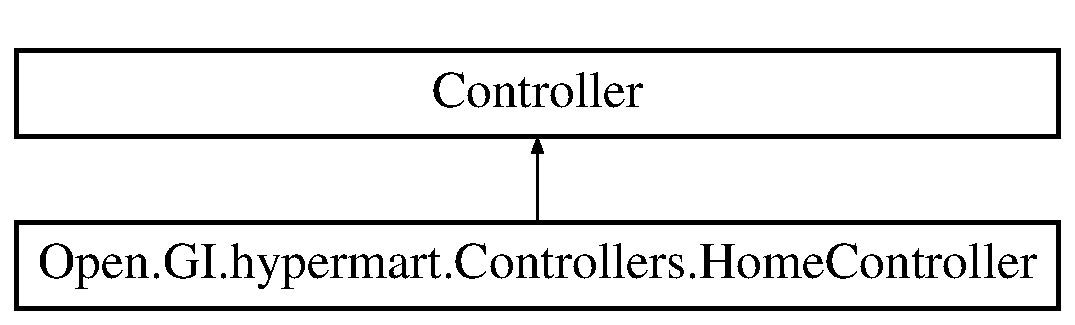
\includegraphics[height=2.000000cm]{class_open_1_1_g_i_1_1hypermart_1_1_controllers_1_1_home_controller}
\end{center}
\end{figure}
\subsection*{Public Member Functions}
\begin{DoxyCompactItemize}
\item 
Action\+Result \hyperlink{class_open_1_1_g_i_1_1hypermart_1_1_controllers_1_1_home_controller_a18ad180258caf702a7cfe51c16bf5558}{Index} ()
\begin{DoxyCompactList}\small\item\em Indexes this instance. \end{DoxyCompactList}\item 
Action\+Result \hyperlink{class_open_1_1_g_i_1_1hypermart_1_1_controllers_1_1_home_controller_a6d90d2a8ae2ce9f7c9ec38b175847e6f}{About} ()
\begin{DoxyCompactList}\small\item\em Abouts this instance. \end{DoxyCompactList}\item 
Action\+Result \hyperlink{class_open_1_1_g_i_1_1hypermart_1_1_controllers_1_1_home_controller_a758666761af826c9091b8a8655eb5e18}{Contact} ()
\begin{DoxyCompactList}\small\item\em Contacts this instance. \end{DoxyCompactList}\end{DoxyCompactItemize}


\subsection{Detailed Description}
A\+S\+P.\+N\+E\+T M\+V\+C Home Controller 

\begin{DoxySeeAlso}{See also}
System.\+Web.\+Mvc.\+Controller


\end{DoxySeeAlso}


Definition at line 13 of file Home\+Controller.\+cs.



\subsection{Member Function Documentation}
\hypertarget{class_open_1_1_g_i_1_1hypermart_1_1_controllers_1_1_home_controller_a6d90d2a8ae2ce9f7c9ec38b175847e6f}{}\index{Open\+::\+G\+I\+::hypermart\+::\+Controllers\+::\+Home\+Controller@{Open\+::\+G\+I\+::hypermart\+::\+Controllers\+::\+Home\+Controller}!About@{About}}
\index{About@{About}!Open\+::\+G\+I\+::hypermart\+::\+Controllers\+::\+Home\+Controller@{Open\+::\+G\+I\+::hypermart\+::\+Controllers\+::\+Home\+Controller}}
\subsubsection[{About()}]{\setlength{\rightskip}{0pt plus 5cm}Action\+Result Open.\+G\+I.\+hypermart.\+Controllers.\+Home\+Controller.\+About (
\begin{DoxyParamCaption}
{}
\end{DoxyParamCaption}
)}\label{class_open_1_1_g_i_1_1hypermart_1_1_controllers_1_1_home_controller_a6d90d2a8ae2ce9f7c9ec38b175847e6f}


Abouts this instance. 

\begin{DoxyReturn}{Returns}

\end{DoxyReturn}


Definition at line 28 of file Home\+Controller.\+cs.

\hypertarget{class_open_1_1_g_i_1_1hypermart_1_1_controllers_1_1_home_controller_a758666761af826c9091b8a8655eb5e18}{}\index{Open\+::\+G\+I\+::hypermart\+::\+Controllers\+::\+Home\+Controller@{Open\+::\+G\+I\+::hypermart\+::\+Controllers\+::\+Home\+Controller}!Contact@{Contact}}
\index{Contact@{Contact}!Open\+::\+G\+I\+::hypermart\+::\+Controllers\+::\+Home\+Controller@{Open\+::\+G\+I\+::hypermart\+::\+Controllers\+::\+Home\+Controller}}
\subsubsection[{Contact()}]{\setlength{\rightskip}{0pt plus 5cm}Action\+Result Open.\+G\+I.\+hypermart.\+Controllers.\+Home\+Controller.\+Contact (
\begin{DoxyParamCaption}
{}
\end{DoxyParamCaption}
)}\label{class_open_1_1_g_i_1_1hypermart_1_1_controllers_1_1_home_controller_a758666761af826c9091b8a8655eb5e18}


Contacts this instance. 

\begin{DoxyReturn}{Returns}

\end{DoxyReturn}


Definition at line 39 of file Home\+Controller.\+cs.

\hypertarget{class_open_1_1_g_i_1_1hypermart_1_1_controllers_1_1_home_controller_a18ad180258caf702a7cfe51c16bf5558}{}\index{Open\+::\+G\+I\+::hypermart\+::\+Controllers\+::\+Home\+Controller@{Open\+::\+G\+I\+::hypermart\+::\+Controllers\+::\+Home\+Controller}!Index@{Index}}
\index{Index@{Index}!Open\+::\+G\+I\+::hypermart\+::\+Controllers\+::\+Home\+Controller@{Open\+::\+G\+I\+::hypermart\+::\+Controllers\+::\+Home\+Controller}}
\subsubsection[{Index()}]{\setlength{\rightskip}{0pt plus 5cm}Action\+Result Open.\+G\+I.\+hypermart.\+Controllers.\+Home\+Controller.\+Index (
\begin{DoxyParamCaption}
{}
\end{DoxyParamCaption}
)}\label{class_open_1_1_g_i_1_1hypermart_1_1_controllers_1_1_home_controller_a18ad180258caf702a7cfe51c16bf5558}


Indexes this instance. 

\begin{DoxyReturn}{Returns}

\end{DoxyReturn}


Definition at line 19 of file Home\+Controller.\+cs.



The documentation for this class was generated from the following file\+:\begin{DoxyCompactItemize}
\item 
C\+:/\+Projects/\+App-\/\+Utility-\/\+Store/\+Open.\+G\+I.\+hypermart/\+Controllers/\hyperlink{_home_controller_8cs}{Home\+Controller.\+cs}\end{DoxyCompactItemize}

\section{Open.\+G\+I.\+hypermart.\+Models.\+Http\+Error\+Page Class Reference}
\label{class_open_1_1_g_i_1_1hypermart_1_1_models_1_1_http_error_page}\index{Open.\+G\+I.\+hypermart.\+Models.\+Http\+Error\+Page@{Open.\+G\+I.\+hypermart.\+Models.\+Http\+Error\+Page}}


Error page information  


\subsection*{Properties}
\begin{DoxyCompactItemize}
\item 
int \textbf{ Error\+Code}\hspace{0.3cm}{\ttfamily  [get, set]}
\begin{DoxyCompactList}\small\item\em Gets or sets the error code. \end{DoxyCompactList}\item 
string \textbf{ Error\+Title}\hspace{0.3cm}{\ttfamily  [get, set]}
\begin{DoxyCompactList}\small\item\em Gets or sets the error title. \end{DoxyCompactList}\item 
string \textbf{ Error\+Description}\hspace{0.3cm}{\ttfamily  [get, set]}
\begin{DoxyCompactList}\small\item\em Gets or sets the error description. \end{DoxyCompactList}\item 
string \textbf{ Technical\+Contact}\hspace{0.3cm}{\ttfamily  [get, set]}
\begin{DoxyCompactList}\small\item\em Gets or sets the technical contact. \end{DoxyCompactList}\end{DoxyCompactItemize}


\subsection{Detailed Description}
Error page information 



Definition at line 12 of file Http\+Error\+Page.\+cs.



\subsection{Property Documentation}
\mbox{\label{class_open_1_1_g_i_1_1hypermart_1_1_models_1_1_http_error_page_a1bf51383a2ce1467237ed44fce2214f0}} 
\index{Open\+::\+G\+I\+::hypermart\+::\+Models\+::\+Http\+Error\+Page@{Open\+::\+G\+I\+::hypermart\+::\+Models\+::\+Http\+Error\+Page}!Error\+Code@{Error\+Code}}
\index{Error\+Code@{Error\+Code}!Open\+::\+G\+I\+::hypermart\+::\+Models\+::\+Http\+Error\+Page@{Open\+::\+G\+I\+::hypermart\+::\+Models\+::\+Http\+Error\+Page}}
\subsubsection{Error\+Code}
{\footnotesize\ttfamily int Open.\+G\+I.\+hypermart.\+Models.\+Http\+Error\+Page.\+Error\+Code\hspace{0.3cm}{\ttfamily [get]}, {\ttfamily [set]}}



Gets or sets the error code. 

The error code. 

Definition at line 20 of file Http\+Error\+Page.\+cs.

\mbox{\label{class_open_1_1_g_i_1_1hypermart_1_1_models_1_1_http_error_page_af5e4bfc21400b65117b1a23090adadb6}} 
\index{Open\+::\+G\+I\+::hypermart\+::\+Models\+::\+Http\+Error\+Page@{Open\+::\+G\+I\+::hypermart\+::\+Models\+::\+Http\+Error\+Page}!Error\+Description@{Error\+Description}}
\index{Error\+Description@{Error\+Description}!Open\+::\+G\+I\+::hypermart\+::\+Models\+::\+Http\+Error\+Page@{Open\+::\+G\+I\+::hypermart\+::\+Models\+::\+Http\+Error\+Page}}
\subsubsection{Error\+Description}
{\footnotesize\ttfamily string Open.\+G\+I.\+hypermart.\+Models.\+Http\+Error\+Page.\+Error\+Description\hspace{0.3cm}{\ttfamily [get]}, {\ttfamily [set]}}



Gets or sets the error description. 

The error description. 

Definition at line 34 of file Http\+Error\+Page.\+cs.

\mbox{\label{class_open_1_1_g_i_1_1hypermart_1_1_models_1_1_http_error_page_a5b8d76394892e084e31faf6781f88d61}} 
\index{Open\+::\+G\+I\+::hypermart\+::\+Models\+::\+Http\+Error\+Page@{Open\+::\+G\+I\+::hypermart\+::\+Models\+::\+Http\+Error\+Page}!Error\+Title@{Error\+Title}}
\index{Error\+Title@{Error\+Title}!Open\+::\+G\+I\+::hypermart\+::\+Models\+::\+Http\+Error\+Page@{Open\+::\+G\+I\+::hypermart\+::\+Models\+::\+Http\+Error\+Page}}
\subsubsection{Error\+Title}
{\footnotesize\ttfamily string Open.\+G\+I.\+hypermart.\+Models.\+Http\+Error\+Page.\+Error\+Title\hspace{0.3cm}{\ttfamily [get]}, {\ttfamily [set]}}



Gets or sets the error title. 

The error title. 

Definition at line 27 of file Http\+Error\+Page.\+cs.

\mbox{\label{class_open_1_1_g_i_1_1hypermart_1_1_models_1_1_http_error_page_a0db493a849f0b8a35064d1c48e736cec}} 
\index{Open\+::\+G\+I\+::hypermart\+::\+Models\+::\+Http\+Error\+Page@{Open\+::\+G\+I\+::hypermart\+::\+Models\+::\+Http\+Error\+Page}!Technical\+Contact@{Technical\+Contact}}
\index{Technical\+Contact@{Technical\+Contact}!Open\+::\+G\+I\+::hypermart\+::\+Models\+::\+Http\+Error\+Page@{Open\+::\+G\+I\+::hypermart\+::\+Models\+::\+Http\+Error\+Page}}
\subsubsection{Technical\+Contact}
{\footnotesize\ttfamily string Open.\+G\+I.\+hypermart.\+Models.\+Http\+Error\+Page.\+Technical\+Contact\hspace{0.3cm}{\ttfamily [get]}, {\ttfamily [set]}}



Gets or sets the technical contact. 

The technical contact. 

Definition at line 41 of file Http\+Error\+Page.\+cs.



The documentation for this class was generated from the following file\+:\begin{DoxyCompactItemize}
\item 
C\+:/\+Projects/\+App-\/\+Utility-\/\+Store/\+Open.\+G\+I.\+hypermart/\+Models/\textbf{ Http\+Error\+Page.\+cs}\end{DoxyCompactItemize}

\hypertarget{class_open_1_1_g_i_1_1hypermart_1_1_d_a_l_1_1_hypermart_context}{}\section{Open.\+G\+I.\+hypermart.\+D\+A\+L.\+Hypermart\+Context Class Reference}
\label{class_open_1_1_g_i_1_1hypermart_1_1_d_a_l_1_1_hypermart_context}\index{Open.\+G\+I.\+hypermart.\+D\+A\+L.\+Hypermart\+Context@{Open.\+G\+I.\+hypermart.\+D\+A\+L.\+Hypermart\+Context}}


Hypermart Context  


Inheritance diagram for Open.\+G\+I.\+hypermart.\+D\+A\+L.\+Hypermart\+Context\+:\begin{figure}[H]
\begin{center}
\leavevmode
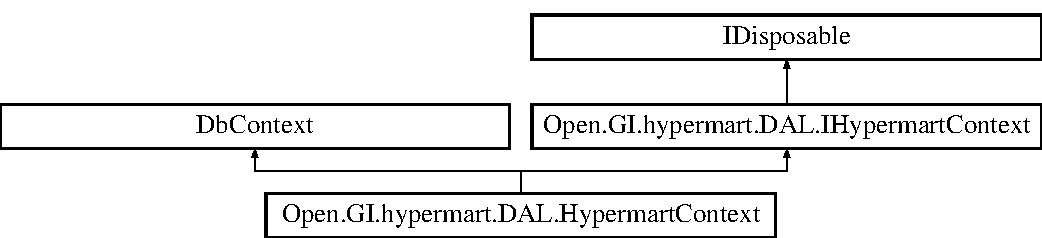
\includegraphics[height=2.000000cm]{class_open_1_1_g_i_1_1hypermart_1_1_d_a_l_1_1_hypermart_context}
\end{center}
\end{figure}
\subsection*{Public Member Functions}
\begin{DoxyCompactItemize}
\item 
\hyperlink{class_open_1_1_g_i_1_1hypermart_1_1_d_a_l_1_1_hypermart_context_a3bcbe3fbf08e41a8b384326b606a7327}{Hypermart\+Context} ()
\begin{DoxyCompactList}\small\item\em Initializes a new instance of the \hyperlink{class_open_1_1_g_i_1_1hypermart_1_1_d_a_l_1_1_hypermart_context}{Hypermart\+Context} class. \end{DoxyCompactList}\item 
new void \hyperlink{class_open_1_1_g_i_1_1hypermart_1_1_d_a_l_1_1_hypermart_context_a30d97828a1a45fcdf9b51cadb10029a4}{Save\+Changes} ()
\begin{DoxyCompactList}\small\item\em In a D\+B Context object, this should save all changes made in this context to the underlying database \end{DoxyCompactList}\end{DoxyCompactItemize}
\subsection*{Protected Member Functions}
\begin{DoxyCompactItemize}
\item 
override void \hyperlink{class_open_1_1_g_i_1_1hypermart_1_1_d_a_l_1_1_hypermart_context_a1a255d0b197dd90f76233146c608a0f1}{On\+Model\+Creating} (Db\+Model\+Builder model\+Builder)
\begin{DoxyCompactList}\small\item\em This method is called when the model for a derived context has been initialized, but before the model has been locked down and used to initialize the context. The default implementation of this method does nothing, but it can be overridden in a derived class such that the model can be further configured before it is locked down. \end{DoxyCompactList}\end{DoxyCompactItemize}
\subsection*{Properties}
\begin{DoxyCompactItemize}
\item 
virtual Db\+Set$<$ \hyperlink{class_open_1_1_g_i_1_1hypermart_1_1_models_1_1_file}{File} $>$ \hyperlink{class_open_1_1_g_i_1_1hypermart_1_1_d_a_l_1_1_hypermart_context_aa42b145ebbfe133c3bc2beddfb23de36}{Files}\hspace{0.3cm}{\ttfamily  \mbox{[}get, set\mbox{]}}
\begin{DoxyCompactList}\small\item\em Gets or sets the files. \end{DoxyCompactList}\item 
virtual Db\+Set$<$ \hyperlink{class_open_1_1_g_i_1_1hypermart_1_1_models_1_1_platform}{Platform} $>$ \hyperlink{class_open_1_1_g_i_1_1hypermart_1_1_d_a_l_1_1_hypermart_context_aff4be9e14ae1b0224c5a7b780050222f}{Platforms}\hspace{0.3cm}{\ttfamily  \mbox{[}get, set\mbox{]}}
\begin{DoxyCompactList}\small\item\em Gets or sets the platforms. \end{DoxyCompactList}\item 
virtual Db\+Set$<$ \hyperlink{class_open_1_1_g_i_1_1hypermart_1_1_models_1_1_product}{Product} $>$ \hyperlink{class_open_1_1_g_i_1_1hypermart_1_1_d_a_l_1_1_hypermart_context_a2673d17b8a620d2f9f11f44edd5d86ef}{Products}\hspace{0.3cm}{\ttfamily  \mbox{[}get, set\mbox{]}}
\begin{DoxyCompactList}\small\item\em Gets or sets the products. \end{DoxyCompactList}\item 
virtual Db\+Set$<$ \hyperlink{class_open_1_1_g_i_1_1hypermart_1_1_models_1_1_screenshot}{Screenshot} $>$ \hyperlink{class_open_1_1_g_i_1_1hypermart_1_1_d_a_l_1_1_hypermart_context_a267136fa00e08f78b49a0a888e548bef}{Screenshots}\hspace{0.3cm}{\ttfamily  \mbox{[}get, set\mbox{]}}
\begin{DoxyCompactList}\small\item\em Gets or sets the screenshots. \end{DoxyCompactList}\end{DoxyCompactItemize}


\subsection{Detailed Description}
Hypermart Context 

\begin{DoxySeeAlso}{See also}
System.\+Data.\+Entity.\+Db\+Context, \hyperlink{interface_open_1_1_g_i_1_1hypermart_1_1_d_a_l_1_1_i_hypermart_context}{Open.\+G\+I.\+hypermart.\+D\+A\+L.\+I\+Hypermart\+Context}


\end{DoxySeeAlso}


Definition at line 14 of file Hypermart\+Context.\+cs.



\subsection{Constructor \& Destructor Documentation}
\hypertarget{class_open_1_1_g_i_1_1hypermart_1_1_d_a_l_1_1_hypermart_context_a3bcbe3fbf08e41a8b384326b606a7327}{}\index{Open\+::\+G\+I\+::hypermart\+::\+D\+A\+L\+::\+Hypermart\+Context@{Open\+::\+G\+I\+::hypermart\+::\+D\+A\+L\+::\+Hypermart\+Context}!Hypermart\+Context@{Hypermart\+Context}}
\index{Hypermart\+Context@{Hypermart\+Context}!Open\+::\+G\+I\+::hypermart\+::\+D\+A\+L\+::\+Hypermart\+Context@{Open\+::\+G\+I\+::hypermart\+::\+D\+A\+L\+::\+Hypermart\+Context}}
\subsubsection[{Hypermart\+Context()}]{\setlength{\rightskip}{0pt plus 5cm}Open.\+G\+I.\+hypermart.\+D\+A\+L.\+Hypermart\+Context.\+Hypermart\+Context (
\begin{DoxyParamCaption}
{}
\end{DoxyParamCaption}
)}\label{class_open_1_1_g_i_1_1hypermart_1_1_d_a_l_1_1_hypermart_context_a3bcbe3fbf08e41a8b384326b606a7327}


Initializes a new instance of the \hyperlink{class_open_1_1_g_i_1_1hypermart_1_1_d_a_l_1_1_hypermart_context}{Hypermart\+Context} class. 



Definition at line 19 of file Hypermart\+Context.\+cs.



\subsection{Member Function Documentation}
\hypertarget{class_open_1_1_g_i_1_1hypermart_1_1_d_a_l_1_1_hypermart_context_a1a255d0b197dd90f76233146c608a0f1}{}\index{Open\+::\+G\+I\+::hypermart\+::\+D\+A\+L\+::\+Hypermart\+Context@{Open\+::\+G\+I\+::hypermart\+::\+D\+A\+L\+::\+Hypermart\+Context}!On\+Model\+Creating@{On\+Model\+Creating}}
\index{On\+Model\+Creating@{On\+Model\+Creating}!Open\+::\+G\+I\+::hypermart\+::\+D\+A\+L\+::\+Hypermart\+Context@{Open\+::\+G\+I\+::hypermart\+::\+D\+A\+L\+::\+Hypermart\+Context}}
\subsubsection[{On\+Model\+Creating(\+Db\+Model\+Builder model\+Builder)}]{\setlength{\rightskip}{0pt plus 5cm}override void Open.\+G\+I.\+hypermart.\+D\+A\+L.\+Hypermart\+Context.\+On\+Model\+Creating (
\begin{DoxyParamCaption}
\item[{Db\+Model\+Builder}]{model\+Builder}
\end{DoxyParamCaption}
)\hspace{0.3cm}{\ttfamily [protected]}}\label{class_open_1_1_g_i_1_1hypermart_1_1_d_a_l_1_1_hypermart_context_a1a255d0b197dd90f76233146c608a0f1}


This method is called when the model for a derived context has been initialized, but before the model has been locked down and used to initialize the context. The default implementation of this method does nothing, but it can be overridden in a derived class such that the model can be further configured before it is locked down. 


\begin{DoxyParams}{Parameters}
{\em model\+Builder} & The builder that defines the model for the context being created.\\
\hline
\end{DoxyParams}


Typically, this method is called only once when the first instance of a derived context is created. The model for that context is then cached and is for all further instances of the context in the app domain. This caching can be disabled by setting the Model\+Caching property on the given Model\+Buidler, but note that this can seriously degrade performance. More control over caching is provided through use of the Db\+Model\+Builder and Db\+Context\+Factory classes directly. 

Definition at line 67 of file Hypermart\+Context.\+cs.

\hypertarget{class_open_1_1_g_i_1_1hypermart_1_1_d_a_l_1_1_hypermart_context_a30d97828a1a45fcdf9b51cadb10029a4}{}\index{Open\+::\+G\+I\+::hypermart\+::\+D\+A\+L\+::\+Hypermart\+Context@{Open\+::\+G\+I\+::hypermart\+::\+D\+A\+L\+::\+Hypermart\+Context}!Save\+Changes@{Save\+Changes}}
\index{Save\+Changes@{Save\+Changes}!Open\+::\+G\+I\+::hypermart\+::\+D\+A\+L\+::\+Hypermart\+Context@{Open\+::\+G\+I\+::hypermart\+::\+D\+A\+L\+::\+Hypermart\+Context}}
\subsubsection[{Save\+Changes()}]{\setlength{\rightskip}{0pt plus 5cm}new void Open.\+G\+I.\+hypermart.\+D\+A\+L.\+Hypermart\+Context.\+Save\+Changes (
\begin{DoxyParamCaption}
{}
\end{DoxyParamCaption}
)}\label{class_open_1_1_g_i_1_1hypermart_1_1_d_a_l_1_1_hypermart_context_a30d97828a1a45fcdf9b51cadb10029a4}


In a D\+B Context object, this should save all changes made in this context to the underlying database 



Implements \hyperlink{interface_open_1_1_g_i_1_1hypermart_1_1_d_a_l_1_1_i_hypermart_context_aacc5015260d97950f2a10d7673873304}{Open.\+G\+I.\+hypermart.\+D\+A\+L.\+I\+Hypermart\+Context}.



Definition at line 84 of file Hypermart\+Context.\+cs.



\subsection{Property Documentation}
\hypertarget{class_open_1_1_g_i_1_1hypermart_1_1_d_a_l_1_1_hypermart_context_aa42b145ebbfe133c3bc2beddfb23de36}{}\index{Open\+::\+G\+I\+::hypermart\+::\+D\+A\+L\+::\+Hypermart\+Context@{Open\+::\+G\+I\+::hypermart\+::\+D\+A\+L\+::\+Hypermart\+Context}!Files@{Files}}
\index{Files@{Files}!Open\+::\+G\+I\+::hypermart\+::\+D\+A\+L\+::\+Hypermart\+Context@{Open\+::\+G\+I\+::hypermart\+::\+D\+A\+L\+::\+Hypermart\+Context}}
\subsubsection[{Files}]{\setlength{\rightskip}{0pt plus 5cm}virtual Db\+Set$<${\bf File}$>$ Open.\+G\+I.\+hypermart.\+D\+A\+L.\+Hypermart\+Context.\+Files\hspace{0.3cm}{\ttfamily [get]}, {\ttfamily [set]}}\label{class_open_1_1_g_i_1_1hypermart_1_1_d_a_l_1_1_hypermart_context_aa42b145ebbfe133c3bc2beddfb23de36}


Gets or sets the files. 

The files. 

Definition at line 29 of file Hypermart\+Context.\+cs.

\hypertarget{class_open_1_1_g_i_1_1hypermart_1_1_d_a_l_1_1_hypermart_context_aff4be9e14ae1b0224c5a7b780050222f}{}\index{Open\+::\+G\+I\+::hypermart\+::\+D\+A\+L\+::\+Hypermart\+Context@{Open\+::\+G\+I\+::hypermart\+::\+D\+A\+L\+::\+Hypermart\+Context}!Platforms@{Platforms}}
\index{Platforms@{Platforms}!Open\+::\+G\+I\+::hypermart\+::\+D\+A\+L\+::\+Hypermart\+Context@{Open\+::\+G\+I\+::hypermart\+::\+D\+A\+L\+::\+Hypermart\+Context}}
\subsubsection[{Platforms}]{\setlength{\rightskip}{0pt plus 5cm}virtual Db\+Set$<${\bf Platform}$>$ Open.\+G\+I.\+hypermart.\+D\+A\+L.\+Hypermart\+Context.\+Platforms\hspace{0.3cm}{\ttfamily [get]}, {\ttfamily [set]}}\label{class_open_1_1_g_i_1_1hypermart_1_1_d_a_l_1_1_hypermart_context_aff4be9e14ae1b0224c5a7b780050222f}


Gets or sets the platforms. 

The platforms. 

Definition at line 36 of file Hypermart\+Context.\+cs.

\hypertarget{class_open_1_1_g_i_1_1hypermart_1_1_d_a_l_1_1_hypermart_context_a2673d17b8a620d2f9f11f44edd5d86ef}{}\index{Open\+::\+G\+I\+::hypermart\+::\+D\+A\+L\+::\+Hypermart\+Context@{Open\+::\+G\+I\+::hypermart\+::\+D\+A\+L\+::\+Hypermart\+Context}!Products@{Products}}
\index{Products@{Products}!Open\+::\+G\+I\+::hypermart\+::\+D\+A\+L\+::\+Hypermart\+Context@{Open\+::\+G\+I\+::hypermart\+::\+D\+A\+L\+::\+Hypermart\+Context}}
\subsubsection[{Products}]{\setlength{\rightskip}{0pt plus 5cm}virtual Db\+Set$<${\bf Product}$>$ Open.\+G\+I.\+hypermart.\+D\+A\+L.\+Hypermart\+Context.\+Products\hspace{0.3cm}{\ttfamily [get]}, {\ttfamily [set]}}\label{class_open_1_1_g_i_1_1hypermart_1_1_d_a_l_1_1_hypermart_context_a2673d17b8a620d2f9f11f44edd5d86ef}


Gets or sets the products. 

The products. 

Definition at line 43 of file Hypermart\+Context.\+cs.

\hypertarget{class_open_1_1_g_i_1_1hypermart_1_1_d_a_l_1_1_hypermart_context_a267136fa00e08f78b49a0a888e548bef}{}\index{Open\+::\+G\+I\+::hypermart\+::\+D\+A\+L\+::\+Hypermart\+Context@{Open\+::\+G\+I\+::hypermart\+::\+D\+A\+L\+::\+Hypermart\+Context}!Screenshots@{Screenshots}}
\index{Screenshots@{Screenshots}!Open\+::\+G\+I\+::hypermart\+::\+D\+A\+L\+::\+Hypermart\+Context@{Open\+::\+G\+I\+::hypermart\+::\+D\+A\+L\+::\+Hypermart\+Context}}
\subsubsection[{Screenshots}]{\setlength{\rightskip}{0pt plus 5cm}virtual Db\+Set$<${\bf Screenshot}$>$ Open.\+G\+I.\+hypermart.\+D\+A\+L.\+Hypermart\+Context.\+Screenshots\hspace{0.3cm}{\ttfamily [get]}, {\ttfamily [set]}}\label{class_open_1_1_g_i_1_1hypermart_1_1_d_a_l_1_1_hypermart_context_a267136fa00e08f78b49a0a888e548bef}


Gets or sets the screenshots. 

The screenshots. 

Definition at line 50 of file Hypermart\+Context.\+cs.



The documentation for this class was generated from the following file\+:\begin{DoxyCompactItemize}
\item 
C\+:/\+Projects/\+App-\/\+Utility-\/\+Store/\+Open.\+G\+I.\+hypermart/\+D\+A\+L/\hyperlink{_hypermart_context_8cs}{Hypermart\+Context.\+cs}\end{DoxyCompactItemize}

\hypertarget{class_open_1_1_g_i_1_1hypermart_1_1_d_a_l_1_1_hypermart_initializer}{}\section{Open.\+G\+I.\+hypermart.\+D\+A\+L.\+Hypermart\+Initializer Class Reference}
\label{class_open_1_1_g_i_1_1hypermart_1_1_d_a_l_1_1_hypermart_initializer}\index{Open.\+G\+I.\+hypermart.\+D\+A\+L.\+Hypermart\+Initializer@{Open.\+G\+I.\+hypermart.\+D\+A\+L.\+Hypermart\+Initializer}}


Hypermart Initializer  


Inheritance diagram for Open.\+G\+I.\+hypermart.\+D\+A\+L.\+Hypermart\+Initializer\+:\begin{figure}[H]
\begin{center}
\leavevmode
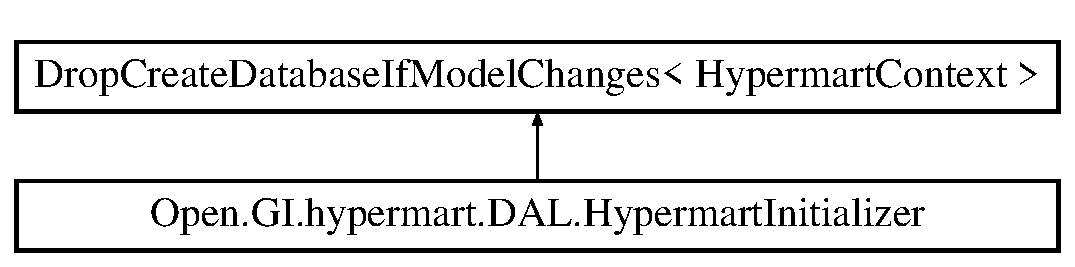
\includegraphics[height=2.000000cm]{class_open_1_1_g_i_1_1hypermart_1_1_d_a_l_1_1_hypermart_initializer}
\end{center}
\end{figure}
\subsection*{Protected Member Functions}
\begin{DoxyCompactItemize}
\item 
override void \hyperlink{class_open_1_1_g_i_1_1hypermart_1_1_d_a_l_1_1_hypermart_initializer_a2e19732fa6f8db0a6b72049415947016}{Seed} (\hyperlink{class_open_1_1_g_i_1_1hypermart_1_1_d_a_l_1_1_hypermart_context}{Hypermart\+Context} context)
\begin{DoxyCompactList}\small\item\em Seeds the database with content. \end{DoxyCompactList}\end{DoxyCompactItemize}


\subsection{Detailed Description}
Hypermart Initializer 



Definition at line 15 of file Hypermart\+Initializer.\+cs.



\subsection{Member Function Documentation}
\hypertarget{class_open_1_1_g_i_1_1hypermart_1_1_d_a_l_1_1_hypermart_initializer_a2e19732fa6f8db0a6b72049415947016}{}\index{Open\+::\+G\+I\+::hypermart\+::\+D\+A\+L\+::\+Hypermart\+Initializer@{Open\+::\+G\+I\+::hypermart\+::\+D\+A\+L\+::\+Hypermart\+Initializer}!Seed@{Seed}}
\index{Seed@{Seed}!Open\+::\+G\+I\+::hypermart\+::\+D\+A\+L\+::\+Hypermart\+Initializer@{Open\+::\+G\+I\+::hypermart\+::\+D\+A\+L\+::\+Hypermart\+Initializer}}
\subsubsection[{Seed(\+Hypermart\+Context context)}]{\setlength{\rightskip}{0pt plus 5cm}override void Open.\+G\+I.\+hypermart.\+D\+A\+L.\+Hypermart\+Initializer.\+Seed (
\begin{DoxyParamCaption}
\item[{{\bf Hypermart\+Context}}]{context}
\end{DoxyParamCaption}
)\hspace{0.3cm}{\ttfamily [protected]}}\label{class_open_1_1_g_i_1_1hypermart_1_1_d_a_l_1_1_hypermart_initializer_a2e19732fa6f8db0a6b72049415947016}


Seeds the database with content. 


\begin{DoxyParams}{Parameters}
{\em context} & The context.\\
\hline
\end{DoxyParams}


Definition at line 21 of file Hypermart\+Initializer.\+cs.



The documentation for this class was generated from the following file\+:\begin{DoxyCompactItemize}
\item 
C\+:/\+Projects/\+App-\/\+Utility-\/\+Store/\+Open.\+G\+I.\+hypermart/\+D\+A\+L/\hyperlink{_hypermart_initializer_8cs}{Hypermart\+Initializer.\+cs}\end{DoxyCompactItemize}

\hypertarget{class_open_1_1_g_i_1_1hypermart_1_1_attributes_1_1_identity_basic_authentication_attribute}{}\section{Open.\+G\+I.\+hypermart.\+Attributes.\+Identity\+Basic\+Authentication\+Attribute Class Reference}
\label{class_open_1_1_g_i_1_1hypermart_1_1_attributes_1_1_identity_basic_authentication_attribute}\index{Open.\+G\+I.\+hypermart.\+Attributes.\+Identity\+Basic\+Authentication\+Attribute@{Open.\+G\+I.\+hypermart.\+Attributes.\+Identity\+Basic\+Authentication\+Attribute}}


Basic Authentication filter for Web\+A\+PI actions  


Inheritance diagram for Open.\+G\+I.\+hypermart.\+Attributes.\+Identity\+Basic\+Authentication\+Attribute\+:\begin{figure}[H]
\begin{center}
\leavevmode
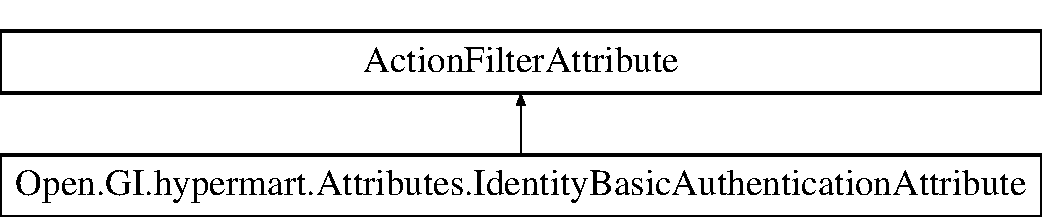
\includegraphics[height=2.000000cm]{class_open_1_1_g_i_1_1hypermart_1_1_attributes_1_1_identity_basic_authentication_attribute}
\end{center}
\end{figure}
\subsection*{Public Member Functions}
\begin{DoxyCompactItemize}
\item 
override void \hyperlink{class_open_1_1_g_i_1_1hypermart_1_1_attributes_1_1_identity_basic_authentication_attribute_af9c5fb2bfb2694f6c284d6f1ec81fc38}{On\+Action\+Executing} (Http\+Action\+Context action\+Context)
\begin{DoxyCompactList}\small\item\em Occurs before the action method is invoked. \end{DoxyCompactList}\end{DoxyCompactItemize}


\subsection{Detailed Description}
Basic Authentication filter for Web\+A\+PI actions 

\begin{DoxySeeAlso}{See also}
System.\+Web.\+Http.\+Filters.\+Action\+Filter\+Attribute


\end{DoxySeeAlso}


\subsection{Member Function Documentation}
\hypertarget{class_open_1_1_g_i_1_1hypermart_1_1_attributes_1_1_identity_basic_authentication_attribute_af9c5fb2bfb2694f6c284d6f1ec81fc38}{}\label{class_open_1_1_g_i_1_1hypermart_1_1_attributes_1_1_identity_basic_authentication_attribute_af9c5fb2bfb2694f6c284d6f1ec81fc38} 
\index{Open\+::\+G\+I\+::hypermart\+::\+Attributes\+::\+Identity\+Basic\+Authentication\+Attribute@{Open\+::\+G\+I\+::hypermart\+::\+Attributes\+::\+Identity\+Basic\+Authentication\+Attribute}!On\+Action\+Executing@{On\+Action\+Executing}}
\index{On\+Action\+Executing@{On\+Action\+Executing}!Open\+::\+G\+I\+::hypermart\+::\+Attributes\+::\+Identity\+Basic\+Authentication\+Attribute@{Open\+::\+G\+I\+::hypermart\+::\+Attributes\+::\+Identity\+Basic\+Authentication\+Attribute}}
\subsubsection{\texorpdfstring{On\+Action\+Executing()}{OnActionExecuting()}}
{\footnotesize\ttfamily override void Open.\+G\+I.\+hypermart.\+Attributes.\+Identity\+Basic\+Authentication\+Attribute.\+On\+Action\+Executing (\begin{DoxyParamCaption}\item[{Http\+Action\+Context}]{action\+Context }\end{DoxyParamCaption})}



Occurs before the action method is invoked. 


\begin{DoxyParams}{Parameters}
{\em action\+Context} & The action context.\\
\hline
\end{DoxyParams}


The documentation for this class was generated from the following file\+:\begin{DoxyCompactItemize}
\item 
C\+:/\+Projects/\+App-\/\+Utility-\/\+Store/\+Open.\+G\+I.\+hypermart/\+Attributes/\hyperlink{_identity_basic_authentication_attribute_8cs}{Identity\+Basic\+Authentication\+Attribute.\+cs}\end{DoxyCompactItemize}

\section{Open.\+G\+I.\+hypermart.\+D\+A\+L.\+I\+Hypermart\+Context Interface Reference}
\label{interface_open_1_1_g_i_1_1hypermart_1_1_d_a_l_1_1_i_hypermart_context}\index{Open.\+G\+I.\+hypermart.\+D\+A\+L.\+I\+Hypermart\+Context@{Open.\+G\+I.\+hypermart.\+D\+A\+L.\+I\+Hypermart\+Context}}


Interface describing the functionality of the Database Context  


Inheritance diagram for Open.\+G\+I.\+hypermart.\+D\+A\+L.\+I\+Hypermart\+Context\+:\begin{figure}[H]
\begin{center}
\leavevmode
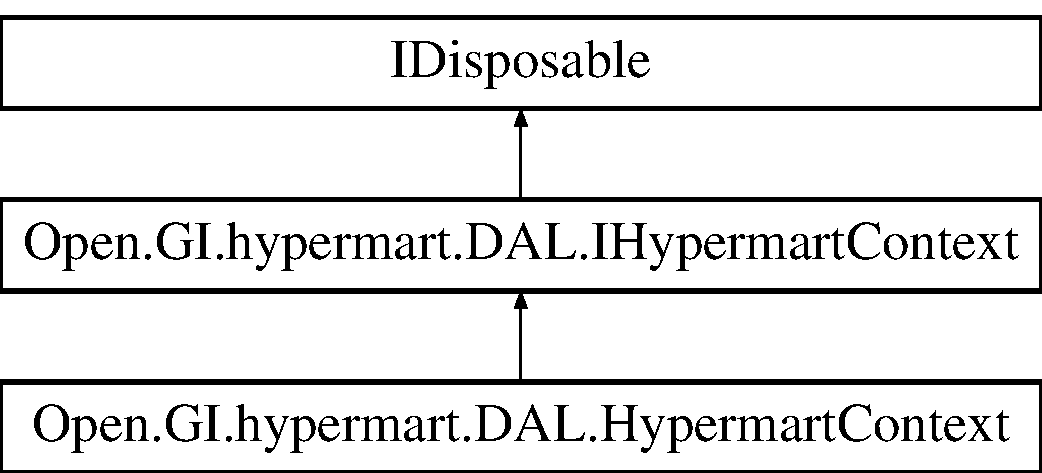
\includegraphics[height=3.000000cm]{interface_open_1_1_g_i_1_1hypermart_1_1_d_a_l_1_1_i_hypermart_context}
\end{center}
\end{figure}
\subsection*{Public Member Functions}
\begin{DoxyCompactItemize}
\item 
void \textbf{ Save\+Changes} ()
\begin{DoxyCompactList}\small\item\em In a DB Context object, this should save all changes made in this context to the underlying database \end{DoxyCompactList}\end{DoxyCompactItemize}
\subsection*{Properties}
\begin{DoxyCompactItemize}
\item 
System.\+Data.\+Entity.\+I\+Db\+Set$<$ \textbf{ Open.\+G\+I.\+hypermart.\+Models.\+File} $>$ \textbf{ Files}\hspace{0.3cm}{\ttfamily  [get, set]}
\begin{DoxyCompactList}\small\item\em Gets or sets the files. \end{DoxyCompactList}\item 
System.\+Data.\+Entity.\+I\+Db\+Set$<$ \textbf{ Open.\+G\+I.\+hypermart.\+Models.\+Platform} $>$ \textbf{ Platforms}\hspace{0.3cm}{\ttfamily  [get, set]}
\begin{DoxyCompactList}\small\item\em Gets or sets the platforms. \end{DoxyCompactList}\item 
System.\+Data.\+Entity.\+I\+Db\+Set$<$ \textbf{ Open.\+G\+I.\+hypermart.\+Models.\+Product} $>$ \textbf{ Products}\hspace{0.3cm}{\ttfamily  [get, set]}
\begin{DoxyCompactList}\small\item\em Gets or sets the products. \end{DoxyCompactList}\item 
System.\+Data.\+Entity.\+I\+Db\+Set$<$ \textbf{ Open.\+G\+I.\+hypermart.\+Models.\+Screenshot} $>$ \textbf{ Screenshots}\hspace{0.3cm}{\ttfamily  [get, set]}
\begin{DoxyCompactList}\small\item\em Gets or sets the screenshots. \end{DoxyCompactList}\item 
System.\+Data.\+Entity.\+I\+Db\+Set$<$ \textbf{ Open.\+G\+I.\+hypermart.\+Models.\+Rating} $>$ \textbf{ Ratings}\hspace{0.3cm}{\ttfamily  [get, set]}
\begin{DoxyCompactList}\small\item\em Gets or sets the ratings. \end{DoxyCompactList}\end{DoxyCompactItemize}


\subsection{Detailed Description}
Interface describing the functionality of the Database Context 



Definition at line 9 of file I\+Hypermart\+Context.\+cs.



\subsection{Member Function Documentation}
\mbox{\label{interface_open_1_1_g_i_1_1hypermart_1_1_d_a_l_1_1_i_hypermart_context_aacc5015260d97950f2a10d7673873304}} 
\index{Open\+::\+G\+I\+::hypermart\+::\+D\+A\+L\+::\+I\+Hypermart\+Context@{Open\+::\+G\+I\+::hypermart\+::\+D\+A\+L\+::\+I\+Hypermart\+Context}!Save\+Changes@{Save\+Changes}}
\index{Save\+Changes@{Save\+Changes}!Open\+::\+G\+I\+::hypermart\+::\+D\+A\+L\+::\+I\+Hypermart\+Context@{Open\+::\+G\+I\+::hypermart\+::\+D\+A\+L\+::\+I\+Hypermart\+Context}}
\subsubsection{Save\+Changes()}
{\footnotesize\ttfamily void Open.\+G\+I.\+hypermart.\+D\+A\+L.\+I\+Hypermart\+Context.\+Save\+Changes (\begin{DoxyParamCaption}{ }\end{DoxyParamCaption})}



In a DB Context object, this should save all changes made in this context to the underlying database 



Implemented in \textbf{ Open.\+G\+I.\+hypermart.\+D\+A\+L.\+Hypermart\+Context} \doxyref{}{p.}{class_open_1_1_g_i_1_1hypermart_1_1_d_a_l_1_1_hypermart_context_a53edb75fbc2507fc97eaf26e36d92f42}.



\subsection{Property Documentation}
\mbox{\label{interface_open_1_1_g_i_1_1hypermart_1_1_d_a_l_1_1_i_hypermart_context_a43675ffb78127ee6af56534c51d593c5}} 
\index{Open\+::\+G\+I\+::hypermart\+::\+D\+A\+L\+::\+I\+Hypermart\+Context@{Open\+::\+G\+I\+::hypermart\+::\+D\+A\+L\+::\+I\+Hypermart\+Context}!Files@{Files}}
\index{Files@{Files}!Open\+::\+G\+I\+::hypermart\+::\+D\+A\+L\+::\+I\+Hypermart\+Context@{Open\+::\+G\+I\+::hypermart\+::\+D\+A\+L\+::\+I\+Hypermart\+Context}}
\subsubsection{Files}
{\footnotesize\ttfamily System.\+Data.\+Entity.\+I\+Db\+Set$<$\textbf{ Open.\+G\+I.\+hypermart.\+Models.\+File}$>$ Open.\+G\+I.\+hypermart.\+D\+A\+L.\+I\+Hypermart\+Context.\+Files\hspace{0.3cm}{\ttfamily [get]}, {\ttfamily [set]}}



Gets or sets the files. 

The files. 

Definition at line 17 of file I\+Hypermart\+Context.\+cs.

\mbox{\label{interface_open_1_1_g_i_1_1hypermart_1_1_d_a_l_1_1_i_hypermart_context_a555845fae4537e83a55b431d87b6642e}} 
\index{Open\+::\+G\+I\+::hypermart\+::\+D\+A\+L\+::\+I\+Hypermart\+Context@{Open\+::\+G\+I\+::hypermart\+::\+D\+A\+L\+::\+I\+Hypermart\+Context}!Platforms@{Platforms}}
\index{Platforms@{Platforms}!Open\+::\+G\+I\+::hypermart\+::\+D\+A\+L\+::\+I\+Hypermart\+Context@{Open\+::\+G\+I\+::hypermart\+::\+D\+A\+L\+::\+I\+Hypermart\+Context}}
\subsubsection{Platforms}
{\footnotesize\ttfamily System.\+Data.\+Entity.\+I\+Db\+Set$<$\textbf{ Open.\+G\+I.\+hypermart.\+Models.\+Platform}$>$ Open.\+G\+I.\+hypermart.\+D\+A\+L.\+I\+Hypermart\+Context.\+Platforms\hspace{0.3cm}{\ttfamily [get]}, {\ttfamily [set]}}



Gets or sets the platforms. 

The platforms. 

Definition at line 24 of file I\+Hypermart\+Context.\+cs.

\mbox{\label{interface_open_1_1_g_i_1_1hypermart_1_1_d_a_l_1_1_i_hypermart_context_addebf65ed282146ad46149f0a4575ec7}} 
\index{Open\+::\+G\+I\+::hypermart\+::\+D\+A\+L\+::\+I\+Hypermart\+Context@{Open\+::\+G\+I\+::hypermart\+::\+D\+A\+L\+::\+I\+Hypermart\+Context}!Products@{Products}}
\index{Products@{Products}!Open\+::\+G\+I\+::hypermart\+::\+D\+A\+L\+::\+I\+Hypermart\+Context@{Open\+::\+G\+I\+::hypermart\+::\+D\+A\+L\+::\+I\+Hypermart\+Context}}
\subsubsection{Products}
{\footnotesize\ttfamily System.\+Data.\+Entity.\+I\+Db\+Set$<$\textbf{ Open.\+G\+I.\+hypermart.\+Models.\+Product}$>$ Open.\+G\+I.\+hypermart.\+D\+A\+L.\+I\+Hypermart\+Context.\+Products\hspace{0.3cm}{\ttfamily [get]}, {\ttfamily [set]}}



Gets or sets the products. 

The products. 

Definition at line 31 of file I\+Hypermart\+Context.\+cs.

\mbox{\label{interface_open_1_1_g_i_1_1hypermart_1_1_d_a_l_1_1_i_hypermart_context_a4e1ab8903a144091a90920c6e3e62d32}} 
\index{Open\+::\+G\+I\+::hypermart\+::\+D\+A\+L\+::\+I\+Hypermart\+Context@{Open\+::\+G\+I\+::hypermart\+::\+D\+A\+L\+::\+I\+Hypermart\+Context}!Ratings@{Ratings}}
\index{Ratings@{Ratings}!Open\+::\+G\+I\+::hypermart\+::\+D\+A\+L\+::\+I\+Hypermart\+Context@{Open\+::\+G\+I\+::hypermart\+::\+D\+A\+L\+::\+I\+Hypermart\+Context}}
\subsubsection{Ratings}
{\footnotesize\ttfamily System.\+Data.\+Entity.\+I\+Db\+Set$<$\textbf{ Open.\+G\+I.\+hypermart.\+Models.\+Rating}$>$ Open.\+G\+I.\+hypermart.\+D\+A\+L.\+I\+Hypermart\+Context.\+Ratings\hspace{0.3cm}{\ttfamily [get]}, {\ttfamily [set]}}



Gets or sets the ratings. 

The ratings. 

Definition at line 45 of file I\+Hypermart\+Context.\+cs.

\mbox{\label{interface_open_1_1_g_i_1_1hypermart_1_1_d_a_l_1_1_i_hypermart_context_ab60981916a8ecd6e871be2f4cb699b19}} 
\index{Open\+::\+G\+I\+::hypermart\+::\+D\+A\+L\+::\+I\+Hypermart\+Context@{Open\+::\+G\+I\+::hypermart\+::\+D\+A\+L\+::\+I\+Hypermart\+Context}!Screenshots@{Screenshots}}
\index{Screenshots@{Screenshots}!Open\+::\+G\+I\+::hypermart\+::\+D\+A\+L\+::\+I\+Hypermart\+Context@{Open\+::\+G\+I\+::hypermart\+::\+D\+A\+L\+::\+I\+Hypermart\+Context}}
\subsubsection{Screenshots}
{\footnotesize\ttfamily System.\+Data.\+Entity.\+I\+Db\+Set$<$\textbf{ Open.\+G\+I.\+hypermart.\+Models.\+Screenshot}$>$ Open.\+G\+I.\+hypermart.\+D\+A\+L.\+I\+Hypermart\+Context.\+Screenshots\hspace{0.3cm}{\ttfamily [get]}, {\ttfamily [set]}}



Gets or sets the screenshots. 

The screenshots. 

Definition at line 38 of file I\+Hypermart\+Context.\+cs.



The documentation for this interface was generated from the following file\+:\begin{DoxyCompactItemize}
\item 
C\+:/\+Projects/\+App-\/\+Utility-\/\+Store/\+Open.\+G\+I.\+hypermart/\+D\+A\+L/\textbf{ I\+Hypermart\+Context.\+cs}\end{DoxyCompactItemize}

\hypertarget{class_open_1_1_g_i_1_1hypermart_1_1_areas_1_1_help_page_1_1_image_sample}{}\section{Open.\+G\+I.\+hypermart.\+Areas.\+Help\+Page.\+Image\+Sample Class Reference}
\label{class_open_1_1_g_i_1_1hypermart_1_1_areas_1_1_help_page_1_1_image_sample}\index{Open.\+G\+I.\+hypermart.\+Areas.\+Help\+Page.\+Image\+Sample@{Open.\+G\+I.\+hypermart.\+Areas.\+Help\+Page.\+Image\+Sample}}


This represents an image sample on the help page. There\textquotesingle{}s a display template named \hyperlink{class_open_1_1_g_i_1_1hypermart_1_1_areas_1_1_help_page_1_1_image_sample}{Image\+Sample} associated with this class.  


\subsection*{Public Member Functions}
\begin{DoxyCompactItemize}
\item 
\hyperlink{class_open_1_1_g_i_1_1hypermart_1_1_areas_1_1_help_page_1_1_image_sample_a3570ac8793e478a72e64041784f39120}{Image\+Sample} (string src)
\begin{DoxyCompactList}\small\item\em Initializes a new instance of the \hyperlink{class_open_1_1_g_i_1_1hypermart_1_1_areas_1_1_help_page_1_1_image_sample}{Image\+Sample} class. \end{DoxyCompactList}\item 
override bool \hyperlink{class_open_1_1_g_i_1_1hypermart_1_1_areas_1_1_help_page_1_1_image_sample_a51e16a01c4f9a5a568c82d1f2d093337}{Equals} (object obj)
\begin{DoxyCompactList}\small\item\em Determines whether the specified System.\+Object, is equal to this instance. \end{DoxyCompactList}\item 
override int \hyperlink{class_open_1_1_g_i_1_1hypermart_1_1_areas_1_1_help_page_1_1_image_sample_a3374507c967e37d7fcba28ec9481865b}{Get\+Hash\+Code} ()
\begin{DoxyCompactList}\small\item\em Returns a hash code for this instance. \end{DoxyCompactList}\item 
override string \hyperlink{class_open_1_1_g_i_1_1hypermart_1_1_areas_1_1_help_page_1_1_image_sample_a704782de956313701ca9e6e61692d433}{To\+String} ()
\begin{DoxyCompactList}\small\item\em Returns a System.\+String that represents this instance. \end{DoxyCompactList}\end{DoxyCompactItemize}
\subsection*{Properties}
\begin{DoxyCompactItemize}
\item 
string \hyperlink{class_open_1_1_g_i_1_1hypermart_1_1_areas_1_1_help_page_1_1_image_sample_a19a1c712823d2e81590e2be51f2e30fb}{Src}\hspace{0.3cm}{\ttfamily  \mbox{[}get\mbox{]}}
\end{DoxyCompactItemize}


\subsection{Detailed Description}
This represents an image sample on the help page. There\textquotesingle{}s a display template named \hyperlink{class_open_1_1_g_i_1_1hypermart_1_1_areas_1_1_help_page_1_1_image_sample}{Image\+Sample} associated with this class. 



\subsection{Constructor \& Destructor Documentation}
\hypertarget{class_open_1_1_g_i_1_1hypermart_1_1_areas_1_1_help_page_1_1_image_sample_a3570ac8793e478a72e64041784f39120}{}\label{class_open_1_1_g_i_1_1hypermart_1_1_areas_1_1_help_page_1_1_image_sample_a3570ac8793e478a72e64041784f39120} 
\index{Open\+::\+G\+I\+::hypermart\+::\+Areas\+::\+Help\+Page\+::\+Image\+Sample@{Open\+::\+G\+I\+::hypermart\+::\+Areas\+::\+Help\+Page\+::\+Image\+Sample}!Image\+Sample@{Image\+Sample}}
\index{Image\+Sample@{Image\+Sample}!Open\+::\+G\+I\+::hypermart\+::\+Areas\+::\+Help\+Page\+::\+Image\+Sample@{Open\+::\+G\+I\+::hypermart\+::\+Areas\+::\+Help\+Page\+::\+Image\+Sample}}
\subsubsection{\texorpdfstring{Image\+Sample()}{ImageSample()}}
{\footnotesize\ttfamily Open.\+G\+I.\+hypermart.\+Areas.\+Help\+Page.\+Image\+Sample.\+Image\+Sample (\begin{DoxyParamCaption}\item[{string}]{src }\end{DoxyParamCaption})}



Initializes a new instance of the \hyperlink{class_open_1_1_g_i_1_1hypermart_1_1_areas_1_1_help_page_1_1_image_sample}{Image\+Sample} class. 


\begin{DoxyParams}{Parameters}
{\em src} & The U\+RL of an image.\\
\hline
\end{DoxyParams}


\subsection{Member Function Documentation}
\hypertarget{class_open_1_1_g_i_1_1hypermart_1_1_areas_1_1_help_page_1_1_image_sample_a51e16a01c4f9a5a568c82d1f2d093337}{}\label{class_open_1_1_g_i_1_1hypermart_1_1_areas_1_1_help_page_1_1_image_sample_a51e16a01c4f9a5a568c82d1f2d093337} 
\index{Open\+::\+G\+I\+::hypermart\+::\+Areas\+::\+Help\+Page\+::\+Image\+Sample@{Open\+::\+G\+I\+::hypermart\+::\+Areas\+::\+Help\+Page\+::\+Image\+Sample}!Equals@{Equals}}
\index{Equals@{Equals}!Open\+::\+G\+I\+::hypermart\+::\+Areas\+::\+Help\+Page\+::\+Image\+Sample@{Open\+::\+G\+I\+::hypermart\+::\+Areas\+::\+Help\+Page\+::\+Image\+Sample}}
\subsubsection{\texorpdfstring{Equals()}{Equals()}}
{\footnotesize\ttfamily override bool Open.\+G\+I.\+hypermart.\+Areas.\+Help\+Page.\+Image\+Sample.\+Equals (\begin{DoxyParamCaption}\item[{object}]{obj }\end{DoxyParamCaption})}



Determines whether the specified System.\+Object, is equal to this instance. 


\begin{DoxyParams}{Parameters}
{\em obj} & The System.\+Object to compare with this instance.\\
\hline
\end{DoxyParams}
\begin{DoxyReturn}{Returns}
{\ttfamily true} if the specified System.\+Object is equal to this instance; otherwise, {\ttfamily false}. 
\end{DoxyReturn}
\hypertarget{class_open_1_1_g_i_1_1hypermart_1_1_areas_1_1_help_page_1_1_image_sample_a3374507c967e37d7fcba28ec9481865b}{}\label{class_open_1_1_g_i_1_1hypermart_1_1_areas_1_1_help_page_1_1_image_sample_a3374507c967e37d7fcba28ec9481865b} 
\index{Open\+::\+G\+I\+::hypermart\+::\+Areas\+::\+Help\+Page\+::\+Image\+Sample@{Open\+::\+G\+I\+::hypermart\+::\+Areas\+::\+Help\+Page\+::\+Image\+Sample}!Get\+Hash\+Code@{Get\+Hash\+Code}}
\index{Get\+Hash\+Code@{Get\+Hash\+Code}!Open\+::\+G\+I\+::hypermart\+::\+Areas\+::\+Help\+Page\+::\+Image\+Sample@{Open\+::\+G\+I\+::hypermart\+::\+Areas\+::\+Help\+Page\+::\+Image\+Sample}}
\subsubsection{\texorpdfstring{Get\+Hash\+Code()}{GetHashCode()}}
{\footnotesize\ttfamily override int Open.\+G\+I.\+hypermart.\+Areas.\+Help\+Page.\+Image\+Sample.\+Get\+Hash\+Code (\begin{DoxyParamCaption}{ }\end{DoxyParamCaption})}



Returns a hash code for this instance. 

\begin{DoxyReturn}{Returns}
A hash code for this instance, suitable for use in hashing algorithms and data structures like a hash table. 
\end{DoxyReturn}
\hypertarget{class_open_1_1_g_i_1_1hypermart_1_1_areas_1_1_help_page_1_1_image_sample_a704782de956313701ca9e6e61692d433}{}\label{class_open_1_1_g_i_1_1hypermart_1_1_areas_1_1_help_page_1_1_image_sample_a704782de956313701ca9e6e61692d433} 
\index{Open\+::\+G\+I\+::hypermart\+::\+Areas\+::\+Help\+Page\+::\+Image\+Sample@{Open\+::\+G\+I\+::hypermart\+::\+Areas\+::\+Help\+Page\+::\+Image\+Sample}!To\+String@{To\+String}}
\index{To\+String@{To\+String}!Open\+::\+G\+I\+::hypermart\+::\+Areas\+::\+Help\+Page\+::\+Image\+Sample@{Open\+::\+G\+I\+::hypermart\+::\+Areas\+::\+Help\+Page\+::\+Image\+Sample}}
\subsubsection{\texorpdfstring{To\+String()}{ToString()}}
{\footnotesize\ttfamily override string Open.\+G\+I.\+hypermart.\+Areas.\+Help\+Page.\+Image\+Sample.\+To\+String (\begin{DoxyParamCaption}{ }\end{DoxyParamCaption})}



Returns a System.\+String that represents this instance. 

\begin{DoxyReturn}{Returns}
A System.\+String that represents this instance. 
\end{DoxyReturn}


\subsection{Property Documentation}
\hypertarget{class_open_1_1_g_i_1_1hypermart_1_1_areas_1_1_help_page_1_1_image_sample_a19a1c712823d2e81590e2be51f2e30fb}{}\label{class_open_1_1_g_i_1_1hypermart_1_1_areas_1_1_help_page_1_1_image_sample_a19a1c712823d2e81590e2be51f2e30fb} 
\index{Open\+::\+G\+I\+::hypermart\+::\+Areas\+::\+Help\+Page\+::\+Image\+Sample@{Open\+::\+G\+I\+::hypermart\+::\+Areas\+::\+Help\+Page\+::\+Image\+Sample}!Src@{Src}}
\index{Src@{Src}!Open\+::\+G\+I\+::hypermart\+::\+Areas\+::\+Help\+Page\+::\+Image\+Sample@{Open\+::\+G\+I\+::hypermart\+::\+Areas\+::\+Help\+Page\+::\+Image\+Sample}}
\subsubsection{\texorpdfstring{Src}{Src}}
{\footnotesize\ttfamily string Open.\+G\+I.\+hypermart.\+Areas.\+Help\+Page.\+Image\+Sample.\+Src\hspace{0.3cm}{\ttfamily [get]}}





The source. 

The documentation for this class was generated from the following file\+:\begin{DoxyCompactItemize}
\item 
C\+:/\+Projects/\+App-\/\+Utility-\/\+Store/\+Open.\+G\+I.\+hypermart/\+Areas/\+Help\+Page/\+Sample\+Generation/\hyperlink{_image_sample_8cs}{Image\+Sample.\+cs}\end{DoxyCompactItemize}

\section{Open.\+G\+I.\+hypermart.\+Areas.\+Help\+Page.\+Model\+Descriptions.\+I\+Model\+Documentation\+Provider Interface Reference}
\label{interface_open_1_1_g_i_1_1hypermart_1_1_areas_1_1_help_page_1_1_model_descriptions_1_1_i_model_documentation_provider}\index{Open.\+G\+I.\+hypermart.\+Areas.\+Help\+Page.\+Model\+Descriptions.\+I\+Model\+Documentation\+Provider@{Open.\+G\+I.\+hypermart.\+Areas.\+Help\+Page.\+Model\+Descriptions.\+I\+Model\+Documentation\+Provider}}


 


Inheritance diagram for Open.\+G\+I.\+hypermart.\+Areas.\+Help\+Page.\+Model\+Descriptions.\+I\+Model\+Documentation\+Provider\+:\begin{figure}[H]
\begin{center}
\leavevmode
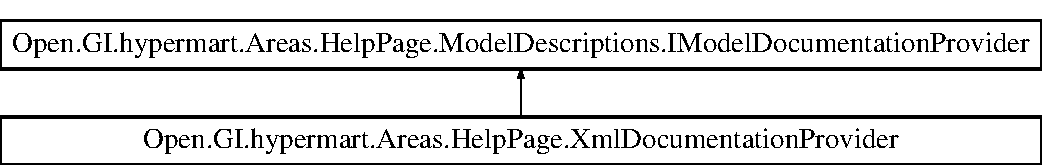
\includegraphics[height=2.000000cm]{interface_open_1_1_g_i_1_1hypermart_1_1_areas_1_1_help_page_1_1_model_descriptions_1_1_i_model_documentation_provider}
\end{center}
\end{figure}
\subsection*{Public Member Functions}
\begin{DoxyCompactItemize}
\item 
string \textbf{ Get\+Documentation} (Member\+Info member)
\begin{DoxyCompactList}\small\item\em Gets the documentation. \end{DoxyCompactList}\item 
string \textbf{ Get\+Documentation} (Type type)
\begin{DoxyCompactList}\small\item\em Gets the documentation. \end{DoxyCompactList}\end{DoxyCompactItemize}


\subsection{Detailed Description}




Definition at line 9 of file I\+Model\+Documentation\+Provider.\+cs.



\subsection{Member Function Documentation}
\mbox{\label{interface_open_1_1_g_i_1_1hypermart_1_1_areas_1_1_help_page_1_1_model_descriptions_1_1_i_model_documentation_provider_a27d4470da05e52051ae345515c17755a}} 
\index{Open\+::\+G\+I\+::hypermart\+::\+Areas\+::\+Help\+Page\+::\+Model\+Descriptions\+::\+I\+Model\+Documentation\+Provider@{Open\+::\+G\+I\+::hypermart\+::\+Areas\+::\+Help\+Page\+::\+Model\+Descriptions\+::\+I\+Model\+Documentation\+Provider}!Get\+Documentation@{Get\+Documentation}}
\index{Get\+Documentation@{Get\+Documentation}!Open\+::\+G\+I\+::hypermart\+::\+Areas\+::\+Help\+Page\+::\+Model\+Descriptions\+::\+I\+Model\+Documentation\+Provider@{Open\+::\+G\+I\+::hypermart\+::\+Areas\+::\+Help\+Page\+::\+Model\+Descriptions\+::\+I\+Model\+Documentation\+Provider}}
\subsubsection{Get\+Documentation()\hspace{0.1cm}{\footnotesize\ttfamily [1/2]}}
{\footnotesize\ttfamily string Open.\+G\+I.\+hypermart.\+Areas.\+Help\+Page.\+Model\+Descriptions.\+I\+Model\+Documentation\+Provider.\+Get\+Documentation (\begin{DoxyParamCaption}\item[{Member\+Info}]{member }\end{DoxyParamCaption})}



Gets the documentation. 


\begin{DoxyParams}{Parameters}
{\em member} & The member.\\
\hline
\end{DoxyParams}
\begin{DoxyReturn}{Returns}

\end{DoxyReturn}


Implemented in \textbf{ Open.\+G\+I.\+hypermart.\+Areas.\+Help\+Page.\+Xml\+Documentation\+Provider} \doxyref{}{p.}{class_open_1_1_g_i_1_1hypermart_1_1_areas_1_1_help_page_1_1_xml_documentation_provider_a1ba7e50dea71787a555f92306ec99efc}.

\mbox{\label{interface_open_1_1_g_i_1_1hypermart_1_1_areas_1_1_help_page_1_1_model_descriptions_1_1_i_model_documentation_provider_a047061b90c62930fc0a1dbcb09732bd3}} 
\index{Open\+::\+G\+I\+::hypermart\+::\+Areas\+::\+Help\+Page\+::\+Model\+Descriptions\+::\+I\+Model\+Documentation\+Provider@{Open\+::\+G\+I\+::hypermart\+::\+Areas\+::\+Help\+Page\+::\+Model\+Descriptions\+::\+I\+Model\+Documentation\+Provider}!Get\+Documentation@{Get\+Documentation}}
\index{Get\+Documentation@{Get\+Documentation}!Open\+::\+G\+I\+::hypermart\+::\+Areas\+::\+Help\+Page\+::\+Model\+Descriptions\+::\+I\+Model\+Documentation\+Provider@{Open\+::\+G\+I\+::hypermart\+::\+Areas\+::\+Help\+Page\+::\+Model\+Descriptions\+::\+I\+Model\+Documentation\+Provider}}
\subsubsection{Get\+Documentation()\hspace{0.1cm}{\footnotesize\ttfamily [2/2]}}
{\footnotesize\ttfamily string Open.\+G\+I.\+hypermart.\+Areas.\+Help\+Page.\+Model\+Descriptions.\+I\+Model\+Documentation\+Provider.\+Get\+Documentation (\begin{DoxyParamCaption}\item[{Type}]{type }\end{DoxyParamCaption})}



Gets the documentation. 


\begin{DoxyParams}{Parameters}
{\em type} & The type.\\
\hline
\end{DoxyParams}
\begin{DoxyReturn}{Returns}

\end{DoxyReturn}


Implemented in \textbf{ Open.\+G\+I.\+hypermart.\+Areas.\+Help\+Page.\+Xml\+Documentation\+Provider} \doxyref{}{p.}{class_open_1_1_g_i_1_1hypermart_1_1_areas_1_1_help_page_1_1_xml_documentation_provider_af096939cdb4e5a26bd20ae3341fad66c}.



The documentation for this interface was generated from the following file\+:\begin{DoxyCompactItemize}
\item 
C\+:/\+Projects/\+App-\/\+Utility-\/\+Store/\+Open.\+G\+I.\+hypermart/\+Areas/\+Help\+Page/\+Model\+Descriptions/\textbf{ I\+Model\+Documentation\+Provider.\+cs}\end{DoxyCompactItemize}

\section{Open.\+G\+I.\+hypermart.\+Migrations.\+Initial Class Reference}
\label{class_open_1_1_g_i_1_1hypermart_1_1_migrations_1_1_initial}\index{Open.\+G\+I.\+hypermart.\+Migrations.\+Initial@{Open.\+G\+I.\+hypermart.\+Migrations.\+Initial}}


 


Inheritance diagram for Open.\+G\+I.\+hypermart.\+Migrations.\+Initial\+:\begin{figure}[H]
\begin{center}
\leavevmode
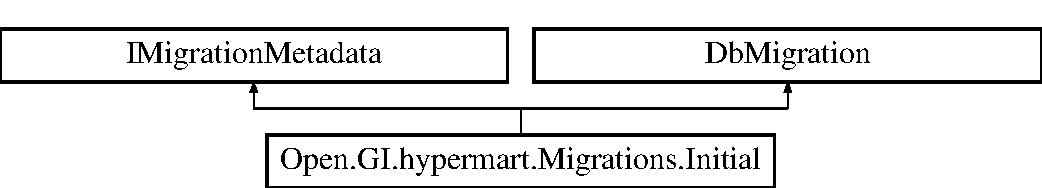
\includegraphics[height=2.000000cm]{class_open_1_1_g_i_1_1hypermart_1_1_migrations_1_1_initial}
\end{center}
\end{figure}
\subsection*{Public Member Functions}
\begin{DoxyCompactItemize}
\item 
override void \textbf{ Up} ()
\begin{DoxyCompactList}\small\item\em Operations to be performed during the upgrade process. \end{DoxyCompactList}\item 
override void \textbf{ Down} ()
\begin{DoxyCompactList}\small\item\em Operations to be performed during the downgrade process. \end{DoxyCompactList}\end{DoxyCompactItemize}


\subsection{Detailed Description}


\begin{DoxySeeAlso}{See also}
System.\+Data.\+Entity.\+Migrations.\+Db\+Migration


\end{DoxySeeAlso}


Definition at line 9 of file 201610201858128\+\_\+\+Initial.\+cs.



\subsection{Member Function Documentation}
\mbox{\label{class_open_1_1_g_i_1_1hypermart_1_1_migrations_1_1_initial_a30a9317e9693d9c0431a1bda53d4497b}} 
\index{Open\+::\+G\+I\+::hypermart\+::\+Migrations\+::\+Initial@{Open\+::\+G\+I\+::hypermart\+::\+Migrations\+::\+Initial}!Down@{Down}}
\index{Down@{Down}!Open\+::\+G\+I\+::hypermart\+::\+Migrations\+::\+Initial@{Open\+::\+G\+I\+::hypermart\+::\+Migrations\+::\+Initial}}
\subsubsection{Down()}
{\footnotesize\ttfamily override void Open.\+G\+I.\+hypermart.\+Migrations.\+Initial.\+Down (\begin{DoxyParamCaption}{ }\end{DoxyParamCaption})}



Operations to be performed during the downgrade process. 



Definition at line 108 of file 201610201858128\+\_\+\+Initial.\+cs.

\mbox{\label{class_open_1_1_g_i_1_1hypermart_1_1_migrations_1_1_initial_a0d322b6e395871e51474b0a1accfa014}} 
\index{Open\+::\+G\+I\+::hypermart\+::\+Migrations\+::\+Initial@{Open\+::\+G\+I\+::hypermart\+::\+Migrations\+::\+Initial}!Up@{Up}}
\index{Up@{Up}!Open\+::\+G\+I\+::hypermart\+::\+Migrations\+::\+Initial@{Open\+::\+G\+I\+::hypermart\+::\+Migrations\+::\+Initial}}
\subsubsection{Up()}
{\footnotesize\ttfamily override void Open.\+G\+I.\+hypermart.\+Migrations.\+Initial.\+Up (\begin{DoxyParamCaption}{ }\end{DoxyParamCaption})}



Operations to be performed during the upgrade process. 



Definition at line 14 of file 201610201858128\+\_\+\+Initial.\+cs.



The documentation for this class was generated from the following files\+:\begin{DoxyCompactItemize}
\item 
C\+:/\+Projects/\+App-\/\+Utility-\/\+Store/\+Open.\+G\+I.\+hypermart/\+Migrations/\textbf{ 201610201858128\+\_\+\+Initial.\+cs}\item 
C\+:/\+Projects/\+App-\/\+Utility-\/\+Store/\+Open.\+G\+I.\+hypermart/\+Migrations/\textbf{ 201610201858128\+\_\+\+Initial.\+Designer.\+cs}\end{DoxyCompactItemize}

\hypertarget{class_open_1_1_g_i_1_1hypermart_1_1_models_1_1_installation_history}{}\section{Open.\+G\+I.\+hypermart.\+Models.\+Installation\+History Class Reference}
\label{class_open_1_1_g_i_1_1hypermart_1_1_models_1_1_installation_history}\index{Open.\+G\+I.\+hypermart.\+Models.\+Installation\+History@{Open.\+G\+I.\+hypermart.\+Models.\+Installation\+History}}


Model object for storing the history of applications that a user has installed.  


\subsection*{Properties}
\begin{DoxyCompactItemize}
\item 
string \hyperlink{class_open_1_1_g_i_1_1hypermart_1_1_models_1_1_installation_history_acfc4d740fbdade68a23eb93a577c9539}{user\+ID}\hspace{0.3cm}{\ttfamily  \mbox{[}get, set\mbox{]}}
\begin{DoxyCompactList}\small\item\em Gets or sets the user identifier. \end{DoxyCompactList}\item 
int \hyperlink{class_open_1_1_g_i_1_1hypermart_1_1_models_1_1_installation_history_a42a9e298540659d4ef03d7bf2440fdae}{Product\+ID}\hspace{0.3cm}{\ttfamily  \mbox{[}get, set\mbox{]}}
\begin{DoxyCompactList}\small\item\em Gets or sets the product identifier. \end{DoxyCompactList}\item 
int \hyperlink{class_open_1_1_g_i_1_1hypermart_1_1_models_1_1_installation_history_ab0b9384f5250f31dc6120af767bfd6ff}{File\+ID}\hspace{0.3cm}{\ttfamily  \mbox{[}get, set\mbox{]}}
\begin{DoxyCompactList}\small\item\em Gets or sets the file identifier. \end{DoxyCompactList}\item 
Date\+Time \hyperlink{class_open_1_1_g_i_1_1hypermart_1_1_models_1_1_installation_history_a6a5b73639b8fabacda9d9661de4ad89c}{Installation\+Date}\hspace{0.3cm}{\ttfamily  \mbox{[}get, set\mbox{]}}
\begin{DoxyCompactList}\small\item\em Date of installation \end{DoxyCompactList}\end{DoxyCompactItemize}


\subsection{Detailed Description}
Model object for storing the history of applications that a user has installed. 



\subsection{Property Documentation}
\hypertarget{class_open_1_1_g_i_1_1hypermart_1_1_models_1_1_installation_history_ab0b9384f5250f31dc6120af767bfd6ff}{}\label{class_open_1_1_g_i_1_1hypermart_1_1_models_1_1_installation_history_ab0b9384f5250f31dc6120af767bfd6ff} 
\index{Open\+::\+G\+I\+::hypermart\+::\+Models\+::\+Installation\+History@{Open\+::\+G\+I\+::hypermart\+::\+Models\+::\+Installation\+History}!File\+ID@{File\+ID}}
\index{File\+ID@{File\+ID}!Open\+::\+G\+I\+::hypermart\+::\+Models\+::\+Installation\+History@{Open\+::\+G\+I\+::hypermart\+::\+Models\+::\+Installation\+History}}
\subsubsection{\texorpdfstring{File\+ID}{FileID}}
{\footnotesize\ttfamily int Open.\+G\+I.\+hypermart.\+Models.\+Installation\+History.\+File\+ID\hspace{0.3cm}{\ttfamily [get]}, {\ttfamily [set]}}



Gets or sets the file identifier. 

The file identifier. \hypertarget{class_open_1_1_g_i_1_1hypermart_1_1_models_1_1_installation_history_a6a5b73639b8fabacda9d9661de4ad89c}{}\label{class_open_1_1_g_i_1_1hypermart_1_1_models_1_1_installation_history_a6a5b73639b8fabacda9d9661de4ad89c} 
\index{Open\+::\+G\+I\+::hypermart\+::\+Models\+::\+Installation\+History@{Open\+::\+G\+I\+::hypermart\+::\+Models\+::\+Installation\+History}!Installation\+Date@{Installation\+Date}}
\index{Installation\+Date@{Installation\+Date}!Open\+::\+G\+I\+::hypermart\+::\+Models\+::\+Installation\+History@{Open\+::\+G\+I\+::hypermart\+::\+Models\+::\+Installation\+History}}
\subsubsection{\texorpdfstring{Installation\+Date}{InstallationDate}}
{\footnotesize\ttfamily Date\+Time Open.\+G\+I.\+hypermart.\+Models.\+Installation\+History.\+Installation\+Date\hspace{0.3cm}{\ttfamily [get]}, {\ttfamily [set]}}



Date of installation 

\hypertarget{class_open_1_1_g_i_1_1hypermart_1_1_models_1_1_installation_history_a42a9e298540659d4ef03d7bf2440fdae}{}\label{class_open_1_1_g_i_1_1hypermart_1_1_models_1_1_installation_history_a42a9e298540659d4ef03d7bf2440fdae} 
\index{Open\+::\+G\+I\+::hypermart\+::\+Models\+::\+Installation\+History@{Open\+::\+G\+I\+::hypermart\+::\+Models\+::\+Installation\+History}!Product\+ID@{Product\+ID}}
\index{Product\+ID@{Product\+ID}!Open\+::\+G\+I\+::hypermart\+::\+Models\+::\+Installation\+History@{Open\+::\+G\+I\+::hypermart\+::\+Models\+::\+Installation\+History}}
\subsubsection{\texorpdfstring{Product\+ID}{ProductID}}
{\footnotesize\ttfamily int Open.\+G\+I.\+hypermart.\+Models.\+Installation\+History.\+Product\+ID\hspace{0.3cm}{\ttfamily [get]}, {\ttfamily [set]}}



Gets or sets the product identifier. 

The product identifier. \hypertarget{class_open_1_1_g_i_1_1hypermart_1_1_models_1_1_installation_history_acfc4d740fbdade68a23eb93a577c9539}{}\label{class_open_1_1_g_i_1_1hypermart_1_1_models_1_1_installation_history_acfc4d740fbdade68a23eb93a577c9539} 
\index{Open\+::\+G\+I\+::hypermart\+::\+Models\+::\+Installation\+History@{Open\+::\+G\+I\+::hypermart\+::\+Models\+::\+Installation\+History}!user\+ID@{user\+ID}}
\index{user\+ID@{user\+ID}!Open\+::\+G\+I\+::hypermart\+::\+Models\+::\+Installation\+History@{Open\+::\+G\+I\+::hypermart\+::\+Models\+::\+Installation\+History}}
\subsubsection{\texorpdfstring{user\+ID}{userID}}
{\footnotesize\ttfamily string Open.\+G\+I.\+hypermart.\+Models.\+Installation\+History.\+user\+ID\hspace{0.3cm}{\ttfamily [get]}, {\ttfamily [set]}}



Gets or sets the user identifier. 

The user identifier. 

The documentation for this class was generated from the following file\+:\begin{DoxyCompactItemize}
\item 
C\+:/\+Projects/\+App-\/\+Utility-\/\+Store/\+Open.\+G\+I.\+hypermart/\+Models/\hyperlink{_installation_history_8cs}{Installation\+History.\+cs}\end{DoxyCompactItemize}

\hypertarget{class_open_1_1_g_i_1_1hypermart_1_1_areas_1_1_help_page_1_1_invalid_sample}{}\section{Open.\+G\+I.\+hypermart.\+Areas.\+Help\+Page.\+Invalid\+Sample Class Reference}
\label{class_open_1_1_g_i_1_1hypermart_1_1_areas_1_1_help_page_1_1_invalid_sample}\index{Open.\+G\+I.\+hypermart.\+Areas.\+Help\+Page.\+Invalid\+Sample@{Open.\+G\+I.\+hypermart.\+Areas.\+Help\+Page.\+Invalid\+Sample}}


This represents an invalid sample on the help page. There\textquotesingle{}s a display template named \hyperlink{class_open_1_1_g_i_1_1hypermart_1_1_areas_1_1_help_page_1_1_invalid_sample}{Invalid\+Sample} associated with this class.  


\subsection*{Public Member Functions}
\begin{DoxyCompactItemize}
\item 
\hyperlink{class_open_1_1_g_i_1_1hypermart_1_1_areas_1_1_help_page_1_1_invalid_sample_a27e0677e2227b94913ea3072e05094b1}{Invalid\+Sample} (string error\+Message)
\begin{DoxyCompactList}\small\item\em Initializes a new instance of the \hyperlink{class_open_1_1_g_i_1_1hypermart_1_1_areas_1_1_help_page_1_1_invalid_sample}{Invalid\+Sample} class. \end{DoxyCompactList}\item 
override bool \hyperlink{class_open_1_1_g_i_1_1hypermart_1_1_areas_1_1_help_page_1_1_invalid_sample_a3c5afe0e3460fccc63bb2b058cf13a8d}{Equals} (object obj)
\begin{DoxyCompactList}\small\item\em Determines whether the specified System.\+Object, is equal to this instance. \end{DoxyCompactList}\item 
override int \hyperlink{class_open_1_1_g_i_1_1hypermart_1_1_areas_1_1_help_page_1_1_invalid_sample_a804d4354478ebcdab08f85e34f138496}{Get\+Hash\+Code} ()
\begin{DoxyCompactList}\small\item\em Returns a hash code for this instance. \end{DoxyCompactList}\item 
override string \hyperlink{class_open_1_1_g_i_1_1hypermart_1_1_areas_1_1_help_page_1_1_invalid_sample_ac19ab8008f61f08252bad6d7c063e7bd}{To\+String} ()
\begin{DoxyCompactList}\small\item\em Returns a System.\+String that represents this instance. \end{DoxyCompactList}\end{DoxyCompactItemize}
\subsection*{Properties}
\begin{DoxyCompactItemize}
\item 
string \hyperlink{class_open_1_1_g_i_1_1hypermart_1_1_areas_1_1_help_page_1_1_invalid_sample_a89f95b69edc57c57963b214d0bc844af}{Error\+Message}\hspace{0.3cm}{\ttfamily  \mbox{[}get\mbox{]}}
\begin{DoxyCompactList}\small\item\em Gets the error message. \end{DoxyCompactList}\end{DoxyCompactItemize}


\subsection{Detailed Description}
This represents an invalid sample on the help page. There\textquotesingle{}s a display template named \hyperlink{class_open_1_1_g_i_1_1hypermart_1_1_areas_1_1_help_page_1_1_invalid_sample}{Invalid\+Sample} associated with this class. 



Definition at line 8 of file Invalid\+Sample.\+cs.



\subsection{Constructor \& Destructor Documentation}
\hypertarget{class_open_1_1_g_i_1_1hypermart_1_1_areas_1_1_help_page_1_1_invalid_sample_a27e0677e2227b94913ea3072e05094b1}{}\index{Open\+::\+G\+I\+::hypermart\+::\+Areas\+::\+Help\+Page\+::\+Invalid\+Sample@{Open\+::\+G\+I\+::hypermart\+::\+Areas\+::\+Help\+Page\+::\+Invalid\+Sample}!Invalid\+Sample@{Invalid\+Sample}}
\index{Invalid\+Sample@{Invalid\+Sample}!Open\+::\+G\+I\+::hypermart\+::\+Areas\+::\+Help\+Page\+::\+Invalid\+Sample@{Open\+::\+G\+I\+::hypermart\+::\+Areas\+::\+Help\+Page\+::\+Invalid\+Sample}}
\subsubsection[{Invalid\+Sample(string error\+Message)}]{\setlength{\rightskip}{0pt plus 5cm}Open.\+G\+I.\+hypermart.\+Areas.\+Help\+Page.\+Invalid\+Sample.\+Invalid\+Sample (
\begin{DoxyParamCaption}
\item[{string}]{error\+Message}
\end{DoxyParamCaption}
)}\label{class_open_1_1_g_i_1_1hypermart_1_1_areas_1_1_help_page_1_1_invalid_sample_a27e0677e2227b94913ea3072e05094b1}


Initializes a new instance of the \hyperlink{class_open_1_1_g_i_1_1hypermart_1_1_areas_1_1_help_page_1_1_invalid_sample}{Invalid\+Sample} class. 


\begin{DoxyParams}{Parameters}
{\em error\+Message} & The error message.\\
\hline
\end{DoxyParams}

\begin{DoxyExceptions}{Exceptions}
{\em System.\+Argument\+Null\+Exception} & error\+Message\\
\hline
\end{DoxyExceptions}


Definition at line 15 of file Invalid\+Sample.\+cs.



\subsection{Member Function Documentation}
\hypertarget{class_open_1_1_g_i_1_1hypermart_1_1_areas_1_1_help_page_1_1_invalid_sample_a3c5afe0e3460fccc63bb2b058cf13a8d}{}\index{Open\+::\+G\+I\+::hypermart\+::\+Areas\+::\+Help\+Page\+::\+Invalid\+Sample@{Open\+::\+G\+I\+::hypermart\+::\+Areas\+::\+Help\+Page\+::\+Invalid\+Sample}!Equals@{Equals}}
\index{Equals@{Equals}!Open\+::\+G\+I\+::hypermart\+::\+Areas\+::\+Help\+Page\+::\+Invalid\+Sample@{Open\+::\+G\+I\+::hypermart\+::\+Areas\+::\+Help\+Page\+::\+Invalid\+Sample}}
\subsubsection[{Equals(object obj)}]{\setlength{\rightskip}{0pt plus 5cm}override bool Open.\+G\+I.\+hypermart.\+Areas.\+Help\+Page.\+Invalid\+Sample.\+Equals (
\begin{DoxyParamCaption}
\item[{object}]{obj}
\end{DoxyParamCaption}
)}\label{class_open_1_1_g_i_1_1hypermart_1_1_areas_1_1_help_page_1_1_invalid_sample_a3c5afe0e3460fccc63bb2b058cf13a8d}


Determines whether the specified System.\+Object, is equal to this instance. 


\begin{DoxyParams}{Parameters}
{\em obj} & The System.\+Object to compare with this instance.\\
\hline
\end{DoxyParams}
\begin{DoxyReturn}{Returns}
{\ttfamily true} if the specified System.\+Object is equal to this instance; otherwise, {\ttfamily false}. 
\end{DoxyReturn}


Definition at line 39 of file Invalid\+Sample.\+cs.

\hypertarget{class_open_1_1_g_i_1_1hypermart_1_1_areas_1_1_help_page_1_1_invalid_sample_a804d4354478ebcdab08f85e34f138496}{}\index{Open\+::\+G\+I\+::hypermart\+::\+Areas\+::\+Help\+Page\+::\+Invalid\+Sample@{Open\+::\+G\+I\+::hypermart\+::\+Areas\+::\+Help\+Page\+::\+Invalid\+Sample}!Get\+Hash\+Code@{Get\+Hash\+Code}}
\index{Get\+Hash\+Code@{Get\+Hash\+Code}!Open\+::\+G\+I\+::hypermart\+::\+Areas\+::\+Help\+Page\+::\+Invalid\+Sample@{Open\+::\+G\+I\+::hypermart\+::\+Areas\+::\+Help\+Page\+::\+Invalid\+Sample}}
\subsubsection[{Get\+Hash\+Code()}]{\setlength{\rightskip}{0pt plus 5cm}override int Open.\+G\+I.\+hypermart.\+Areas.\+Help\+Page.\+Invalid\+Sample.\+Get\+Hash\+Code (
\begin{DoxyParamCaption}
{}
\end{DoxyParamCaption}
)}\label{class_open_1_1_g_i_1_1hypermart_1_1_areas_1_1_help_page_1_1_invalid_sample_a804d4354478ebcdab08f85e34f138496}


Returns a hash code for this instance. 

\begin{DoxyReturn}{Returns}
A hash code for this instance, suitable for use in hashing algorithms and data structures like a hash table. 
\end{DoxyReturn}


Definition at line 51 of file Invalid\+Sample.\+cs.

\hypertarget{class_open_1_1_g_i_1_1hypermart_1_1_areas_1_1_help_page_1_1_invalid_sample_ac19ab8008f61f08252bad6d7c063e7bd}{}\index{Open\+::\+G\+I\+::hypermart\+::\+Areas\+::\+Help\+Page\+::\+Invalid\+Sample@{Open\+::\+G\+I\+::hypermart\+::\+Areas\+::\+Help\+Page\+::\+Invalid\+Sample}!To\+String@{To\+String}}
\index{To\+String@{To\+String}!Open\+::\+G\+I\+::hypermart\+::\+Areas\+::\+Help\+Page\+::\+Invalid\+Sample@{Open\+::\+G\+I\+::hypermart\+::\+Areas\+::\+Help\+Page\+::\+Invalid\+Sample}}
\subsubsection[{To\+String()}]{\setlength{\rightskip}{0pt plus 5cm}override string Open.\+G\+I.\+hypermart.\+Areas.\+Help\+Page.\+Invalid\+Sample.\+To\+String (
\begin{DoxyParamCaption}
{}
\end{DoxyParamCaption}
)}\label{class_open_1_1_g_i_1_1hypermart_1_1_areas_1_1_help_page_1_1_invalid_sample_ac19ab8008f61f08252bad6d7c063e7bd}


Returns a System.\+String that represents this instance. 

\begin{DoxyReturn}{Returns}
A System.\+String that represents this instance. 
\end{DoxyReturn}


Definition at line 62 of file Invalid\+Sample.\+cs.



\subsection{Property Documentation}
\hypertarget{class_open_1_1_g_i_1_1hypermart_1_1_areas_1_1_help_page_1_1_invalid_sample_a89f95b69edc57c57963b214d0bc844af}{}\index{Open\+::\+G\+I\+::hypermart\+::\+Areas\+::\+Help\+Page\+::\+Invalid\+Sample@{Open\+::\+G\+I\+::hypermart\+::\+Areas\+::\+Help\+Page\+::\+Invalid\+Sample}!Error\+Message@{Error\+Message}}
\index{Error\+Message@{Error\+Message}!Open\+::\+G\+I\+::hypermart\+::\+Areas\+::\+Help\+Page\+::\+Invalid\+Sample@{Open\+::\+G\+I\+::hypermart\+::\+Areas\+::\+Help\+Page\+::\+Invalid\+Sample}}
\subsubsection[{Error\+Message}]{\setlength{\rightskip}{0pt plus 5cm}string Open.\+G\+I.\+hypermart.\+Areas.\+Help\+Page.\+Invalid\+Sample.\+Error\+Message\hspace{0.3cm}{\ttfamily [get]}}\label{class_open_1_1_g_i_1_1hypermart_1_1_areas_1_1_help_page_1_1_invalid_sample_a89f95b69edc57c57963b214d0bc844af}


Gets the error message. 

The error message. 

Definition at line 30 of file Invalid\+Sample.\+cs.



The documentation for this class was generated from the following file\+:\begin{DoxyCompactItemize}
\item 
C\+:/\+Projects/\+App-\/\+Utility-\/\+Store/\+Open.\+G\+I.\+hypermart/\+Areas/\+Help\+Page/\+Sample\+Generation/\hyperlink{_invalid_sample_8cs}{Invalid\+Sample.\+cs}\end{DoxyCompactItemize}

\hypertarget{class_open_1_1_g_i_1_1hypermart_1_1_areas_1_1_help_page_1_1_model_descriptions_1_1_key_value_pair_model_description}{}\section{Open.\+G\+I.\+hypermart.\+Areas.\+Help\+Page.\+Model\+Descriptions.\+Key\+Value\+Pair\+Model\+Description Class Reference}
\label{class_open_1_1_g_i_1_1hypermart_1_1_areas_1_1_help_page_1_1_model_descriptions_1_1_key_value_pair_model_description}\index{Open.\+G\+I.\+hypermart.\+Areas.\+Help\+Page.\+Model\+Descriptions.\+Key\+Value\+Pair\+Model\+Description@{Open.\+G\+I.\+hypermart.\+Areas.\+Help\+Page.\+Model\+Descriptions.\+Key\+Value\+Pair\+Model\+Description}}


 


Inheritance diagram for Open.\+G\+I.\+hypermart.\+Areas.\+Help\+Page.\+Model\+Descriptions.\+Key\+Value\+Pair\+Model\+Description\+:\begin{figure}[H]
\begin{center}
\leavevmode
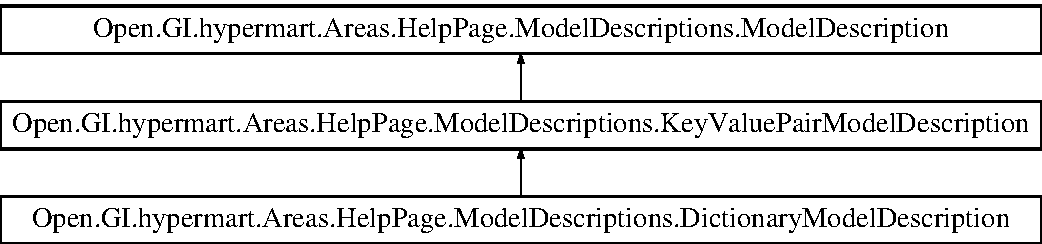
\includegraphics[height=3.000000cm]{class_open_1_1_g_i_1_1hypermart_1_1_areas_1_1_help_page_1_1_model_descriptions_1_1_key_value_pair_model_description}
\end{center}
\end{figure}
\subsection*{Properties}
\begin{DoxyCompactItemize}
\item 
\hyperlink{class_open_1_1_g_i_1_1hypermart_1_1_areas_1_1_help_page_1_1_model_descriptions_1_1_model_description}{Model\+Description} \hyperlink{class_open_1_1_g_i_1_1hypermart_1_1_areas_1_1_help_page_1_1_model_descriptions_1_1_key_value_pair_model_description_a76ccd9d3ad532ce5a56b52d15d84c324}{Key\+Model\+Description}\hspace{0.3cm}{\ttfamily  \mbox{[}get, set\mbox{]}}
\begin{DoxyCompactList}\small\item\em Gets or sets the key model description. \end{DoxyCompactList}\item 
\hyperlink{class_open_1_1_g_i_1_1hypermart_1_1_areas_1_1_help_page_1_1_model_descriptions_1_1_model_description}{Model\+Description} \hyperlink{class_open_1_1_g_i_1_1hypermart_1_1_areas_1_1_help_page_1_1_model_descriptions_1_1_key_value_pair_model_description_a5bcf18b1e78df6ba8b0cbc001a11ace6}{Value\+Model\+Description}\hspace{0.3cm}{\ttfamily  \mbox{[}get, set\mbox{]}}
\begin{DoxyCompactList}\small\item\em Gets or sets the value model description. \end{DoxyCompactList}\end{DoxyCompactItemize}


\subsection{Detailed Description}


\begin{DoxySeeAlso}{See also}
\hyperlink{class_open_1_1_g_i_1_1hypermart_1_1_areas_1_1_help_page_1_1_model_descriptions_1_1_model_description}{Open.\+G\+I.\+hypermart.\+Areas.\+Help\+Page.\+Model\+Descriptions.\+Model\+Description}


\end{DoxySeeAlso}


\subsection{Property Documentation}
\hypertarget{class_open_1_1_g_i_1_1hypermart_1_1_areas_1_1_help_page_1_1_model_descriptions_1_1_key_value_pair_model_description_a76ccd9d3ad532ce5a56b52d15d84c324}{}\label{class_open_1_1_g_i_1_1hypermart_1_1_areas_1_1_help_page_1_1_model_descriptions_1_1_key_value_pair_model_description_a76ccd9d3ad532ce5a56b52d15d84c324} 
\index{Open\+::\+G\+I\+::hypermart\+::\+Areas\+::\+Help\+Page\+::\+Model\+Descriptions\+::\+Key\+Value\+Pair\+Model\+Description@{Open\+::\+G\+I\+::hypermart\+::\+Areas\+::\+Help\+Page\+::\+Model\+Descriptions\+::\+Key\+Value\+Pair\+Model\+Description}!Key\+Model\+Description@{Key\+Model\+Description}}
\index{Key\+Model\+Description@{Key\+Model\+Description}!Open\+::\+G\+I\+::hypermart\+::\+Areas\+::\+Help\+Page\+::\+Model\+Descriptions\+::\+Key\+Value\+Pair\+Model\+Description@{Open\+::\+G\+I\+::hypermart\+::\+Areas\+::\+Help\+Page\+::\+Model\+Descriptions\+::\+Key\+Value\+Pair\+Model\+Description}}
\subsubsection{\texorpdfstring{Key\+Model\+Description}{KeyModelDescription}}
{\footnotesize\ttfamily \hyperlink{class_open_1_1_g_i_1_1hypermart_1_1_areas_1_1_help_page_1_1_model_descriptions_1_1_model_description}{Model\+Description} Open.\+G\+I.\+hypermart.\+Areas.\+Help\+Page.\+Model\+Descriptions.\+Key\+Value\+Pair\+Model\+Description.\+Key\+Model\+Description\hspace{0.3cm}{\ttfamily [get]}, {\ttfamily [set]}}



Gets or sets the key model description. 

The key model description. \hypertarget{class_open_1_1_g_i_1_1hypermart_1_1_areas_1_1_help_page_1_1_model_descriptions_1_1_key_value_pair_model_description_a5bcf18b1e78df6ba8b0cbc001a11ace6}{}\label{class_open_1_1_g_i_1_1hypermart_1_1_areas_1_1_help_page_1_1_model_descriptions_1_1_key_value_pair_model_description_a5bcf18b1e78df6ba8b0cbc001a11ace6} 
\index{Open\+::\+G\+I\+::hypermart\+::\+Areas\+::\+Help\+Page\+::\+Model\+Descriptions\+::\+Key\+Value\+Pair\+Model\+Description@{Open\+::\+G\+I\+::hypermart\+::\+Areas\+::\+Help\+Page\+::\+Model\+Descriptions\+::\+Key\+Value\+Pair\+Model\+Description}!Value\+Model\+Description@{Value\+Model\+Description}}
\index{Value\+Model\+Description@{Value\+Model\+Description}!Open\+::\+G\+I\+::hypermart\+::\+Areas\+::\+Help\+Page\+::\+Model\+Descriptions\+::\+Key\+Value\+Pair\+Model\+Description@{Open\+::\+G\+I\+::hypermart\+::\+Areas\+::\+Help\+Page\+::\+Model\+Descriptions\+::\+Key\+Value\+Pair\+Model\+Description}}
\subsubsection{\texorpdfstring{Value\+Model\+Description}{ValueModelDescription}}
{\footnotesize\ttfamily \hyperlink{class_open_1_1_g_i_1_1hypermart_1_1_areas_1_1_help_page_1_1_model_descriptions_1_1_model_description}{Model\+Description} Open.\+G\+I.\+hypermart.\+Areas.\+Help\+Page.\+Model\+Descriptions.\+Key\+Value\+Pair\+Model\+Description.\+Value\+Model\+Description\hspace{0.3cm}{\ttfamily [get]}, {\ttfamily [set]}}



Gets or sets the value model description. 

The value model description. 

The documentation for this class was generated from the following file\+:\begin{DoxyCompactItemize}
\item 
C\+:/\+Projects/\+App-\/\+Utility-\/\+Store/\+Open.\+G\+I.\+hypermart/\+Areas/\+Help\+Page/\+Model\+Descriptions/\hyperlink{_key_value_pair_model_description_8cs}{Key\+Value\+Pair\+Model\+Description.\+cs}\end{DoxyCompactItemize}

\hypertarget{class_open_1_1_g_i_1_1hypermart_1_1_models_1_1_model1_container}{}\section{Open.\+G\+I.\+hypermart.\+Models.\+Model1\+Container Class Reference}
\label{class_open_1_1_g_i_1_1hypermart_1_1_models_1_1_model1_container}\index{Open.\+G\+I.\+hypermart.\+Models.\+Model1\+Container@{Open.\+G\+I.\+hypermart.\+Models.\+Model1\+Container}}
Inheritance diagram for Open.\+G\+I.\+hypermart.\+Models.\+Model1\+Container\+:\begin{figure}[H]
\begin{center}
\leavevmode
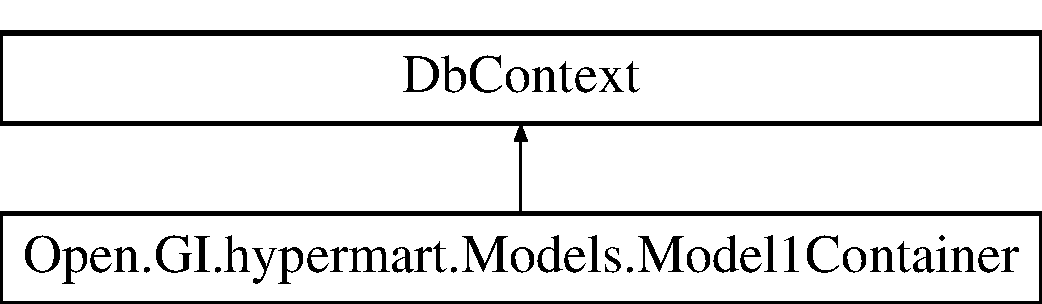
\includegraphics[height=2.000000cm]{class_open_1_1_g_i_1_1hypermart_1_1_models_1_1_model1_container}
\end{center}
\end{figure}
\subsection*{Public Member Functions}
\begin{DoxyCompactItemize}
\item 
\hyperlink{class_open_1_1_g_i_1_1hypermart_1_1_models_1_1_model1_container_a8d957335d29c47427c9d9062c11e6205}{Model1\+Container} ()
\end{DoxyCompactItemize}
\subsection*{Protected Member Functions}
\begin{DoxyCompactItemize}
\item 
override void \hyperlink{class_open_1_1_g_i_1_1hypermart_1_1_models_1_1_model1_container_a738eaf983c5fc89665bff3d90f9fb188}{On\+Model\+Creating} (Db\+Model\+Builder model\+Builder)
\end{DoxyCompactItemize}
\subsection*{Properties}
\begin{DoxyCompactItemize}
\item 
virtual Db\+Set$<$ \hyperlink{class_open_1_1_g_i_1_1hypermart_1_1_models_1_1_file}{File} $>$ \hyperlink{class_open_1_1_g_i_1_1hypermart_1_1_models_1_1_model1_container_a446f391e8b281cf4e3e71f369940189c}{Files}\hspace{0.3cm}{\ttfamily  \mbox{[}get, set\mbox{]}}
\item 
virtual Db\+Set$<$ \hyperlink{class_open_1_1_g_i_1_1hypermart_1_1_models_1_1_file_platform}{File\+Platform} $>$ \hyperlink{class_open_1_1_g_i_1_1hypermart_1_1_models_1_1_model1_container_ad8999f3ba131f3c46c9162b2eff4c7f9}{File\+Platforms}\hspace{0.3cm}{\ttfamily  \mbox{[}get, set\mbox{]}}
\item 
virtual Db\+Set$<$ \hyperlink{class_open_1_1_g_i_1_1hypermart_1_1_models_1_1_platform}{Platform} $>$ \hyperlink{class_open_1_1_g_i_1_1hypermart_1_1_models_1_1_model1_container_a47b249679414da9e63797516568ddb73}{Platforms}\hspace{0.3cm}{\ttfamily  \mbox{[}get, set\mbox{]}}
\item 
virtual Db\+Set$<$ \hyperlink{class_open_1_1_g_i_1_1hypermart_1_1_models_1_1_product}{Product} $>$ \hyperlink{class_open_1_1_g_i_1_1hypermart_1_1_models_1_1_model1_container_a3152c9cb162bad57e707fb1a6b48152c}{Products}\hspace{0.3cm}{\ttfamily  \mbox{[}get, set\mbox{]}}
\item 
virtual Db\+Set$<$ \hyperlink{class_open_1_1_g_i_1_1hypermart_1_1_models_1_1_screenshot}{Screenshot} $>$ \hyperlink{class_open_1_1_g_i_1_1hypermart_1_1_models_1_1_model1_container_a16840948ed271ebac66728f3398b6696}{Screenshots}\hspace{0.3cm}{\ttfamily  \mbox{[}get, set\mbox{]}}
\end{DoxyCompactItemize}


\subsection{Detailed Description}


Definition at line 16 of file Model1.\+Context.\+cs.



\subsection{Constructor \& Destructor Documentation}
\hypertarget{class_open_1_1_g_i_1_1hypermart_1_1_models_1_1_model1_container_a8d957335d29c47427c9d9062c11e6205}{}\index{Open\+::\+G\+I\+::hypermart\+::\+Models\+::\+Model1\+Container@{Open\+::\+G\+I\+::hypermart\+::\+Models\+::\+Model1\+Container}!Model1\+Container@{Model1\+Container}}
\index{Model1\+Container@{Model1\+Container}!Open\+::\+G\+I\+::hypermart\+::\+Models\+::\+Model1\+Container@{Open\+::\+G\+I\+::hypermart\+::\+Models\+::\+Model1\+Container}}
\subsubsection[{Model1\+Container()}]{\setlength{\rightskip}{0pt plus 5cm}Open.\+G\+I.\+hypermart.\+Models.\+Model1\+Container.\+Model1\+Container (
\begin{DoxyParamCaption}
{}
\end{DoxyParamCaption}
)}\label{class_open_1_1_g_i_1_1hypermart_1_1_models_1_1_model1_container_a8d957335d29c47427c9d9062c11e6205}


Definition at line 18 of file Model1.\+Context.\+cs.



\subsection{Member Function Documentation}
\hypertarget{class_open_1_1_g_i_1_1hypermart_1_1_models_1_1_model1_container_a738eaf983c5fc89665bff3d90f9fb188}{}\index{Open\+::\+G\+I\+::hypermart\+::\+Models\+::\+Model1\+Container@{Open\+::\+G\+I\+::hypermart\+::\+Models\+::\+Model1\+Container}!On\+Model\+Creating@{On\+Model\+Creating}}
\index{On\+Model\+Creating@{On\+Model\+Creating}!Open\+::\+G\+I\+::hypermart\+::\+Models\+::\+Model1\+Container@{Open\+::\+G\+I\+::hypermart\+::\+Models\+::\+Model1\+Container}}
\subsubsection[{On\+Model\+Creating(\+Db\+Model\+Builder model\+Builder)}]{\setlength{\rightskip}{0pt plus 5cm}override void Open.\+G\+I.\+hypermart.\+Models.\+Model1\+Container.\+On\+Model\+Creating (
\begin{DoxyParamCaption}
\item[{Db\+Model\+Builder}]{model\+Builder}
\end{DoxyParamCaption}
)\hspace{0.3cm}{\ttfamily [protected]}}\label{class_open_1_1_g_i_1_1hypermart_1_1_models_1_1_model1_container_a738eaf983c5fc89665bff3d90f9fb188}


Definition at line 23 of file Model1.\+Context.\+cs.



\subsection{Property Documentation}
\hypertarget{class_open_1_1_g_i_1_1hypermart_1_1_models_1_1_model1_container_ad8999f3ba131f3c46c9162b2eff4c7f9}{}\index{Open\+::\+G\+I\+::hypermart\+::\+Models\+::\+Model1\+Container@{Open\+::\+G\+I\+::hypermart\+::\+Models\+::\+Model1\+Container}!File\+Platforms@{File\+Platforms}}
\index{File\+Platforms@{File\+Platforms}!Open\+::\+G\+I\+::hypermart\+::\+Models\+::\+Model1\+Container@{Open\+::\+G\+I\+::hypermart\+::\+Models\+::\+Model1\+Container}}
\subsubsection[{File\+Platforms}]{\setlength{\rightskip}{0pt plus 5cm}virtual Db\+Set$<${\bf File\+Platform}$>$ Open.\+G\+I.\+hypermart.\+Models.\+Model1\+Container.\+File\+Platforms\hspace{0.3cm}{\ttfamily [get]}, {\ttfamily [set]}}\label{class_open_1_1_g_i_1_1hypermart_1_1_models_1_1_model1_container_ad8999f3ba131f3c46c9162b2eff4c7f9}


Definition at line 29 of file Model1.\+Context.\+cs.

\hypertarget{class_open_1_1_g_i_1_1hypermart_1_1_models_1_1_model1_container_a446f391e8b281cf4e3e71f369940189c}{}\index{Open\+::\+G\+I\+::hypermart\+::\+Models\+::\+Model1\+Container@{Open\+::\+G\+I\+::hypermart\+::\+Models\+::\+Model1\+Container}!Files@{Files}}
\index{Files@{Files}!Open\+::\+G\+I\+::hypermart\+::\+Models\+::\+Model1\+Container@{Open\+::\+G\+I\+::hypermart\+::\+Models\+::\+Model1\+Container}}
\subsubsection[{Files}]{\setlength{\rightskip}{0pt plus 5cm}virtual Db\+Set$<${\bf File}$>$ Open.\+G\+I.\+hypermart.\+Models.\+Model1\+Container.\+Files\hspace{0.3cm}{\ttfamily [get]}, {\ttfamily [set]}}\label{class_open_1_1_g_i_1_1hypermart_1_1_models_1_1_model1_container_a446f391e8b281cf4e3e71f369940189c}


Definition at line 28 of file Model1.\+Context.\+cs.

\hypertarget{class_open_1_1_g_i_1_1hypermart_1_1_models_1_1_model1_container_a47b249679414da9e63797516568ddb73}{}\index{Open\+::\+G\+I\+::hypermart\+::\+Models\+::\+Model1\+Container@{Open\+::\+G\+I\+::hypermart\+::\+Models\+::\+Model1\+Container}!Platforms@{Platforms}}
\index{Platforms@{Platforms}!Open\+::\+G\+I\+::hypermart\+::\+Models\+::\+Model1\+Container@{Open\+::\+G\+I\+::hypermart\+::\+Models\+::\+Model1\+Container}}
\subsubsection[{Platforms}]{\setlength{\rightskip}{0pt plus 5cm}virtual Db\+Set$<${\bf Platform}$>$ Open.\+G\+I.\+hypermart.\+Models.\+Model1\+Container.\+Platforms\hspace{0.3cm}{\ttfamily [get]}, {\ttfamily [set]}}\label{class_open_1_1_g_i_1_1hypermart_1_1_models_1_1_model1_container_a47b249679414da9e63797516568ddb73}


Definition at line 30 of file Model1.\+Context.\+cs.

\hypertarget{class_open_1_1_g_i_1_1hypermart_1_1_models_1_1_model1_container_a3152c9cb162bad57e707fb1a6b48152c}{}\index{Open\+::\+G\+I\+::hypermart\+::\+Models\+::\+Model1\+Container@{Open\+::\+G\+I\+::hypermart\+::\+Models\+::\+Model1\+Container}!Products@{Products}}
\index{Products@{Products}!Open\+::\+G\+I\+::hypermart\+::\+Models\+::\+Model1\+Container@{Open\+::\+G\+I\+::hypermart\+::\+Models\+::\+Model1\+Container}}
\subsubsection[{Products}]{\setlength{\rightskip}{0pt plus 5cm}virtual Db\+Set$<${\bf Product}$>$ Open.\+G\+I.\+hypermart.\+Models.\+Model1\+Container.\+Products\hspace{0.3cm}{\ttfamily [get]}, {\ttfamily [set]}}\label{class_open_1_1_g_i_1_1hypermart_1_1_models_1_1_model1_container_a3152c9cb162bad57e707fb1a6b48152c}


Definition at line 31 of file Model1.\+Context.\+cs.

\hypertarget{class_open_1_1_g_i_1_1hypermart_1_1_models_1_1_model1_container_a16840948ed271ebac66728f3398b6696}{}\index{Open\+::\+G\+I\+::hypermart\+::\+Models\+::\+Model1\+Container@{Open\+::\+G\+I\+::hypermart\+::\+Models\+::\+Model1\+Container}!Screenshots@{Screenshots}}
\index{Screenshots@{Screenshots}!Open\+::\+G\+I\+::hypermart\+::\+Models\+::\+Model1\+Container@{Open\+::\+G\+I\+::hypermart\+::\+Models\+::\+Model1\+Container}}
\subsubsection[{Screenshots}]{\setlength{\rightskip}{0pt plus 5cm}virtual Db\+Set$<${\bf Screenshot}$>$ Open.\+G\+I.\+hypermart.\+Models.\+Model1\+Container.\+Screenshots\hspace{0.3cm}{\ttfamily [get]}, {\ttfamily [set]}}\label{class_open_1_1_g_i_1_1hypermart_1_1_models_1_1_model1_container_a16840948ed271ebac66728f3398b6696}


Definition at line 32 of file Model1.\+Context.\+cs.



The documentation for this class was generated from the following file\+:\begin{DoxyCompactItemize}
\item 
C\+:/\+Projects/\+App-\/\+Utility-\/\+Store/\+Open.\+G\+I.\+hypermart/\+W\+I\+P/\hyperlink{_model1_8_context_8cs}{Model1.\+Context.\+cs}\end{DoxyCompactItemize}

\hypertarget{class_open_1_1_g_i_1_1hypermart_1_1_areas_1_1_help_page_1_1_model_descriptions_1_1_model_description}{}\section{Open.\+G\+I.\+hypermart.\+Areas.\+Help\+Page.\+Model\+Descriptions.\+Model\+Description Class Reference}
\label{class_open_1_1_g_i_1_1hypermart_1_1_areas_1_1_help_page_1_1_model_descriptions_1_1_model_description}\index{Open.\+G\+I.\+hypermart.\+Areas.\+Help\+Page.\+Model\+Descriptions.\+Model\+Description@{Open.\+G\+I.\+hypermart.\+Areas.\+Help\+Page.\+Model\+Descriptions.\+Model\+Description}}


Describes a type model.  


Inheritance diagram for Open.\+G\+I.\+hypermart.\+Areas.\+Help\+Page.\+Model\+Descriptions.\+Model\+Description\+:\begin{figure}[H]
\begin{center}
\leavevmode
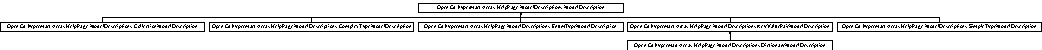
\includegraphics[height=0.652427cm]{class_open_1_1_g_i_1_1hypermart_1_1_areas_1_1_help_page_1_1_model_descriptions_1_1_model_description}
\end{center}
\end{figure}
\subsection*{Properties}
\begin{DoxyCompactItemize}
\item 
string \hyperlink{class_open_1_1_g_i_1_1hypermart_1_1_areas_1_1_help_page_1_1_model_descriptions_1_1_model_description_af08e1f5a6e3a28669b602926cb9a07b9}{Documentation}\hspace{0.3cm}{\ttfamily  \mbox{[}get, set\mbox{]}}
\begin{DoxyCompactList}\small\item\em Gets or sets the documentation. \end{DoxyCompactList}\item 
Type \hyperlink{class_open_1_1_g_i_1_1hypermart_1_1_areas_1_1_help_page_1_1_model_descriptions_1_1_model_description_ab41d4f322450e3a2cde611673ca4abb1}{Model\+Type}\hspace{0.3cm}{\ttfamily  \mbox{[}get, set\mbox{]}}
\begin{DoxyCompactList}\small\item\em Gets or sets the type of the model. \end{DoxyCompactList}\item 
string \hyperlink{class_open_1_1_g_i_1_1hypermart_1_1_areas_1_1_help_page_1_1_model_descriptions_1_1_model_description_aa5a42ec74b1d880ce15fd12b8ef0baf9}{Name}\hspace{0.3cm}{\ttfamily  \mbox{[}get, set\mbox{]}}
\begin{DoxyCompactList}\small\item\em Gets or sets the name. \end{DoxyCompactList}\end{DoxyCompactItemize}


\subsection{Detailed Description}
Describes a type model. 



\subsection{Property Documentation}
\hypertarget{class_open_1_1_g_i_1_1hypermart_1_1_areas_1_1_help_page_1_1_model_descriptions_1_1_model_description_af08e1f5a6e3a28669b602926cb9a07b9}{}\label{class_open_1_1_g_i_1_1hypermart_1_1_areas_1_1_help_page_1_1_model_descriptions_1_1_model_description_af08e1f5a6e3a28669b602926cb9a07b9} 
\index{Open\+::\+G\+I\+::hypermart\+::\+Areas\+::\+Help\+Page\+::\+Model\+Descriptions\+::\+Model\+Description@{Open\+::\+G\+I\+::hypermart\+::\+Areas\+::\+Help\+Page\+::\+Model\+Descriptions\+::\+Model\+Description}!Documentation@{Documentation}}
\index{Documentation@{Documentation}!Open\+::\+G\+I\+::hypermart\+::\+Areas\+::\+Help\+Page\+::\+Model\+Descriptions\+::\+Model\+Description@{Open\+::\+G\+I\+::hypermart\+::\+Areas\+::\+Help\+Page\+::\+Model\+Descriptions\+::\+Model\+Description}}
\subsubsection{\texorpdfstring{Documentation}{Documentation}}
{\footnotesize\ttfamily string Open.\+G\+I.\+hypermart.\+Areas.\+Help\+Page.\+Model\+Descriptions.\+Model\+Description.\+Documentation\hspace{0.3cm}{\ttfamily [get]}, {\ttfamily [set]}}



Gets or sets the documentation. 

The documentation. \hypertarget{class_open_1_1_g_i_1_1hypermart_1_1_areas_1_1_help_page_1_1_model_descriptions_1_1_model_description_ab41d4f322450e3a2cde611673ca4abb1}{}\label{class_open_1_1_g_i_1_1hypermart_1_1_areas_1_1_help_page_1_1_model_descriptions_1_1_model_description_ab41d4f322450e3a2cde611673ca4abb1} 
\index{Open\+::\+G\+I\+::hypermart\+::\+Areas\+::\+Help\+Page\+::\+Model\+Descriptions\+::\+Model\+Description@{Open\+::\+G\+I\+::hypermart\+::\+Areas\+::\+Help\+Page\+::\+Model\+Descriptions\+::\+Model\+Description}!Model\+Type@{Model\+Type}}
\index{Model\+Type@{Model\+Type}!Open\+::\+G\+I\+::hypermart\+::\+Areas\+::\+Help\+Page\+::\+Model\+Descriptions\+::\+Model\+Description@{Open\+::\+G\+I\+::hypermart\+::\+Areas\+::\+Help\+Page\+::\+Model\+Descriptions\+::\+Model\+Description}}
\subsubsection{\texorpdfstring{Model\+Type}{ModelType}}
{\footnotesize\ttfamily Type Open.\+G\+I.\+hypermart.\+Areas.\+Help\+Page.\+Model\+Descriptions.\+Model\+Description.\+Model\+Type\hspace{0.3cm}{\ttfamily [get]}, {\ttfamily [set]}}



Gets or sets the type of the model. 

The type of the model. \hypertarget{class_open_1_1_g_i_1_1hypermart_1_1_areas_1_1_help_page_1_1_model_descriptions_1_1_model_description_aa5a42ec74b1d880ce15fd12b8ef0baf9}{}\label{class_open_1_1_g_i_1_1hypermart_1_1_areas_1_1_help_page_1_1_model_descriptions_1_1_model_description_aa5a42ec74b1d880ce15fd12b8ef0baf9} 
\index{Open\+::\+G\+I\+::hypermart\+::\+Areas\+::\+Help\+Page\+::\+Model\+Descriptions\+::\+Model\+Description@{Open\+::\+G\+I\+::hypermart\+::\+Areas\+::\+Help\+Page\+::\+Model\+Descriptions\+::\+Model\+Description}!Name@{Name}}
\index{Name@{Name}!Open\+::\+G\+I\+::hypermart\+::\+Areas\+::\+Help\+Page\+::\+Model\+Descriptions\+::\+Model\+Description@{Open\+::\+G\+I\+::hypermart\+::\+Areas\+::\+Help\+Page\+::\+Model\+Descriptions\+::\+Model\+Description}}
\subsubsection{\texorpdfstring{Name}{Name}}
{\footnotesize\ttfamily string Open.\+G\+I.\+hypermart.\+Areas.\+Help\+Page.\+Model\+Descriptions.\+Model\+Description.\+Name\hspace{0.3cm}{\ttfamily [get]}, {\ttfamily [set]}}



Gets or sets the name. 

The name. 

The documentation for this class was generated from the following file\+:\begin{DoxyCompactItemize}
\item 
C\+:/\+Projects/\+App-\/\+Utility-\/\+Store/\+Open.\+G\+I.\+hypermart/\+Areas/\+Help\+Page/\+Model\+Descriptions/\hyperlink{_model_description_8cs}{Model\+Description.\+cs}\end{DoxyCompactItemize}

\hypertarget{class_open_1_1_g_i_1_1hypermart_1_1_areas_1_1_help_page_1_1_model_descriptions_1_1_model_description_generator}{}\section{Open.\+G\+I.\+hypermart.\+Areas.\+Help\+Page.\+Model\+Descriptions.\+Model\+Description\+Generator Class Reference}
\label{class_open_1_1_g_i_1_1hypermart_1_1_areas_1_1_help_page_1_1_model_descriptions_1_1_model_description_generator}\index{Open.\+G\+I.\+hypermart.\+Areas.\+Help\+Page.\+Model\+Descriptions.\+Model\+Description\+Generator@{Open.\+G\+I.\+hypermart.\+Areas.\+Help\+Page.\+Model\+Descriptions.\+Model\+Description\+Generator}}


Generates model descriptions for given types.  


\subsection*{Public Member Functions}
\begin{DoxyCompactItemize}
\item 
\hyperlink{class_open_1_1_g_i_1_1hypermart_1_1_areas_1_1_help_page_1_1_model_descriptions_1_1_model_description_generator_a56c6ca4b29667cf648929f4bbedca964}{Model\+Description\+Generator} (Http\+Configuration config)
\begin{DoxyCompactList}\small\item\em Initializes a new instance of the \hyperlink{class_open_1_1_g_i_1_1hypermart_1_1_areas_1_1_help_page_1_1_model_descriptions_1_1_model_description_generator}{Model\+Description\+Generator} class. \end{DoxyCompactList}\item 
\hyperlink{class_open_1_1_g_i_1_1hypermart_1_1_areas_1_1_help_page_1_1_model_descriptions_1_1_model_description}{Model\+Description} \hyperlink{class_open_1_1_g_i_1_1hypermart_1_1_areas_1_1_help_page_1_1_model_descriptions_1_1_model_description_generator_aa693e668d64aa73688aaa4fc080eb525}{Get\+Or\+Create\+Model\+Description} (Type model\+Type)
\begin{DoxyCompactList}\small\item\em Gets the or create model description. \end{DoxyCompactList}\end{DoxyCompactItemize}
\subsection*{Properties}
\begin{DoxyCompactItemize}
\item 
Dictionary$<$ string, \hyperlink{class_open_1_1_g_i_1_1hypermart_1_1_areas_1_1_help_page_1_1_model_descriptions_1_1_model_description}{Model\+Description} $>$ \hyperlink{class_open_1_1_g_i_1_1hypermart_1_1_areas_1_1_help_page_1_1_model_descriptions_1_1_model_description_generator_ad4d703c3da52e11a1e52c12ae04e88a6}{Generated\+Models}\hspace{0.3cm}{\ttfamily  \mbox{[}get\mbox{]}}
\begin{DoxyCompactList}\small\item\em Gets the generated models. \end{DoxyCompactList}\end{DoxyCompactItemize}


\subsection{Detailed Description}
Generates model descriptions for given types. 



\subsection{Constructor \& Destructor Documentation}
\hypertarget{class_open_1_1_g_i_1_1hypermart_1_1_areas_1_1_help_page_1_1_model_descriptions_1_1_model_description_generator_a56c6ca4b29667cf648929f4bbedca964}{}\label{class_open_1_1_g_i_1_1hypermart_1_1_areas_1_1_help_page_1_1_model_descriptions_1_1_model_description_generator_a56c6ca4b29667cf648929f4bbedca964} 
\index{Open\+::\+G\+I\+::hypermart\+::\+Areas\+::\+Help\+Page\+::\+Model\+Descriptions\+::\+Model\+Description\+Generator@{Open\+::\+G\+I\+::hypermart\+::\+Areas\+::\+Help\+Page\+::\+Model\+Descriptions\+::\+Model\+Description\+Generator}!Model\+Description\+Generator@{Model\+Description\+Generator}}
\index{Model\+Description\+Generator@{Model\+Description\+Generator}!Open\+::\+G\+I\+::hypermart\+::\+Areas\+::\+Help\+Page\+::\+Model\+Descriptions\+::\+Model\+Description\+Generator@{Open\+::\+G\+I\+::hypermart\+::\+Areas\+::\+Help\+Page\+::\+Model\+Descriptions\+::\+Model\+Description\+Generator}}
\subsubsection{\texorpdfstring{Model\+Description\+Generator()}{ModelDescriptionGenerator()}}
{\footnotesize\ttfamily Open.\+G\+I.\+hypermart.\+Areas.\+Help\+Page.\+Model\+Descriptions.\+Model\+Description\+Generator.\+Model\+Description\+Generator (\begin{DoxyParamCaption}\item[{Http\+Configuration}]{config }\end{DoxyParamCaption})}



Initializes a new instance of the \hyperlink{class_open_1_1_g_i_1_1hypermart_1_1_areas_1_1_help_page_1_1_model_descriptions_1_1_model_description_generator}{Model\+Description\+Generator} class. 


\begin{DoxyParams}{Parameters}
{\em config} & The configuration.\\
\hline
\end{DoxyParams}


\subsection{Member Function Documentation}
\hypertarget{class_open_1_1_g_i_1_1hypermart_1_1_areas_1_1_help_page_1_1_model_descriptions_1_1_model_description_generator_aa693e668d64aa73688aaa4fc080eb525}{}\label{class_open_1_1_g_i_1_1hypermart_1_1_areas_1_1_help_page_1_1_model_descriptions_1_1_model_description_generator_aa693e668d64aa73688aaa4fc080eb525} 
\index{Open\+::\+G\+I\+::hypermart\+::\+Areas\+::\+Help\+Page\+::\+Model\+Descriptions\+::\+Model\+Description\+Generator@{Open\+::\+G\+I\+::hypermart\+::\+Areas\+::\+Help\+Page\+::\+Model\+Descriptions\+::\+Model\+Description\+Generator}!Get\+Or\+Create\+Model\+Description@{Get\+Or\+Create\+Model\+Description}}
\index{Get\+Or\+Create\+Model\+Description@{Get\+Or\+Create\+Model\+Description}!Open\+::\+G\+I\+::hypermart\+::\+Areas\+::\+Help\+Page\+::\+Model\+Descriptions\+::\+Model\+Description\+Generator@{Open\+::\+G\+I\+::hypermart\+::\+Areas\+::\+Help\+Page\+::\+Model\+Descriptions\+::\+Model\+Description\+Generator}}
\subsubsection{\texorpdfstring{Get\+Or\+Create\+Model\+Description()}{GetOrCreateModelDescription()}}
{\footnotesize\ttfamily \hyperlink{class_open_1_1_g_i_1_1hypermart_1_1_areas_1_1_help_page_1_1_model_descriptions_1_1_model_description}{Model\+Description} Open.\+G\+I.\+hypermart.\+Areas.\+Help\+Page.\+Model\+Descriptions.\+Model\+Description\+Generator.\+Get\+Or\+Create\+Model\+Description (\begin{DoxyParamCaption}\item[{Type}]{model\+Type }\end{DoxyParamCaption})}



Gets the or create model description. 


\begin{DoxyParams}{Parameters}
{\em model\+Type} & Type of the model.\\
\hline
\end{DoxyParams}
\begin{DoxyReturn}{Returns}

\end{DoxyReturn}


\subsection{Property Documentation}
\hypertarget{class_open_1_1_g_i_1_1hypermart_1_1_areas_1_1_help_page_1_1_model_descriptions_1_1_model_description_generator_ad4d703c3da52e11a1e52c12ae04e88a6}{}\label{class_open_1_1_g_i_1_1hypermart_1_1_areas_1_1_help_page_1_1_model_descriptions_1_1_model_description_generator_ad4d703c3da52e11a1e52c12ae04e88a6} 
\index{Open\+::\+G\+I\+::hypermart\+::\+Areas\+::\+Help\+Page\+::\+Model\+Descriptions\+::\+Model\+Description\+Generator@{Open\+::\+G\+I\+::hypermart\+::\+Areas\+::\+Help\+Page\+::\+Model\+Descriptions\+::\+Model\+Description\+Generator}!Generated\+Models@{Generated\+Models}}
\index{Generated\+Models@{Generated\+Models}!Open\+::\+G\+I\+::hypermart\+::\+Areas\+::\+Help\+Page\+::\+Model\+Descriptions\+::\+Model\+Description\+Generator@{Open\+::\+G\+I\+::hypermart\+::\+Areas\+::\+Help\+Page\+::\+Model\+Descriptions\+::\+Model\+Description\+Generator}}
\subsubsection{\texorpdfstring{Generated\+Models}{GeneratedModels}}
{\footnotesize\ttfamily Dictionary$<$string, \hyperlink{class_open_1_1_g_i_1_1hypermart_1_1_areas_1_1_help_page_1_1_model_descriptions_1_1_model_description}{Model\+Description}$>$ Open.\+G\+I.\+hypermart.\+Areas.\+Help\+Page.\+Model\+Descriptions.\+Model\+Description\+Generator.\+Generated\+Models\hspace{0.3cm}{\ttfamily [get]}}



Gets the generated models. 

The generated models. 

The documentation for this class was generated from the following file\+:\begin{DoxyCompactItemize}
\item 
C\+:/\+Projects/\+App-\/\+Utility-\/\+Store/\+Open.\+G\+I.\+hypermart/\+Areas/\+Help\+Page/\+Model\+Descriptions/\hyperlink{_model_description_generator_8cs}{Model\+Description\+Generator.\+cs}\end{DoxyCompactItemize}

\hypertarget{class_open_1_1_g_i_1_1hypermart_1_1_areas_1_1_help_page_1_1_model_descriptions_1_1_model_name_attribute}{}\section{Open.\+G\+I.\+hypermart.\+Areas.\+Help\+Page.\+Model\+Descriptions.\+Model\+Name\+Attribute Class Reference}
\label{class_open_1_1_g_i_1_1hypermart_1_1_areas_1_1_help_page_1_1_model_descriptions_1_1_model_name_attribute}\index{Open.\+G\+I.\+hypermart.\+Areas.\+Help\+Page.\+Model\+Descriptions.\+Model\+Name\+Attribute@{Open.\+G\+I.\+hypermart.\+Areas.\+Help\+Page.\+Model\+Descriptions.\+Model\+Name\+Attribute}}


Use this attribute to change the name of the \hyperlink{class_open_1_1_g_i_1_1hypermart_1_1_areas_1_1_help_page_1_1_model_descriptions_1_1_model_description}{Model\+Description} generated for a type.  


Inheritance diagram for Open.\+G\+I.\+hypermart.\+Areas.\+Help\+Page.\+Model\+Descriptions.\+Model\+Name\+Attribute\+:\begin{figure}[H]
\begin{center}
\leavevmode
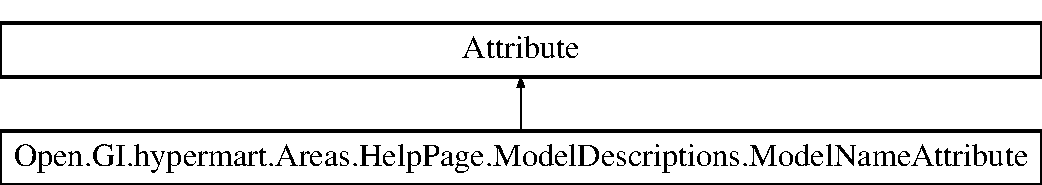
\includegraphics[height=2.000000cm]{class_open_1_1_g_i_1_1hypermart_1_1_areas_1_1_help_page_1_1_model_descriptions_1_1_model_name_attribute}
\end{center}
\end{figure}
\subsection*{Public Member Functions}
\begin{DoxyCompactItemize}
\item 
\hyperlink{class_open_1_1_g_i_1_1hypermart_1_1_areas_1_1_help_page_1_1_model_descriptions_1_1_model_name_attribute_a993a54c4cc771558eef5ea586b70d6d7}{Model\+Name\+Attribute} (string name)
\begin{DoxyCompactList}\small\item\em Initializes a new instance of the \hyperlink{class_open_1_1_g_i_1_1hypermart_1_1_areas_1_1_help_page_1_1_model_descriptions_1_1_model_name_attribute}{Model\+Name\+Attribute} class. \end{DoxyCompactList}\end{DoxyCompactItemize}
\subsection*{Properties}
\begin{DoxyCompactItemize}
\item 
string \hyperlink{class_open_1_1_g_i_1_1hypermart_1_1_areas_1_1_help_page_1_1_model_descriptions_1_1_model_name_attribute_a1388599f97bb13f4b52da9cebfd994d3}{Name}\hspace{0.3cm}{\ttfamily  \mbox{[}get\mbox{]}}
\begin{DoxyCompactList}\small\item\em Gets the name. \end{DoxyCompactList}\end{DoxyCompactItemize}


\subsection{Detailed Description}
Use this attribute to change the name of the \hyperlink{class_open_1_1_g_i_1_1hypermart_1_1_areas_1_1_help_page_1_1_model_descriptions_1_1_model_description}{Model\+Description} generated for a type. 



\subsection{Constructor \& Destructor Documentation}
\hypertarget{class_open_1_1_g_i_1_1hypermart_1_1_areas_1_1_help_page_1_1_model_descriptions_1_1_model_name_attribute_a993a54c4cc771558eef5ea586b70d6d7}{}\label{class_open_1_1_g_i_1_1hypermart_1_1_areas_1_1_help_page_1_1_model_descriptions_1_1_model_name_attribute_a993a54c4cc771558eef5ea586b70d6d7} 
\index{Open\+::\+G\+I\+::hypermart\+::\+Areas\+::\+Help\+Page\+::\+Model\+Descriptions\+::\+Model\+Name\+Attribute@{Open\+::\+G\+I\+::hypermart\+::\+Areas\+::\+Help\+Page\+::\+Model\+Descriptions\+::\+Model\+Name\+Attribute}!Model\+Name\+Attribute@{Model\+Name\+Attribute}}
\index{Model\+Name\+Attribute@{Model\+Name\+Attribute}!Open\+::\+G\+I\+::hypermart\+::\+Areas\+::\+Help\+Page\+::\+Model\+Descriptions\+::\+Model\+Name\+Attribute@{Open\+::\+G\+I\+::hypermart\+::\+Areas\+::\+Help\+Page\+::\+Model\+Descriptions\+::\+Model\+Name\+Attribute}}
\subsubsection{\texorpdfstring{Model\+Name\+Attribute()}{ModelNameAttribute()}}
{\footnotesize\ttfamily Open.\+G\+I.\+hypermart.\+Areas.\+Help\+Page.\+Model\+Descriptions.\+Model\+Name\+Attribute.\+Model\+Name\+Attribute (\begin{DoxyParamCaption}\item[{string}]{name }\end{DoxyParamCaption})}



Initializes a new instance of the \hyperlink{class_open_1_1_g_i_1_1hypermart_1_1_areas_1_1_help_page_1_1_model_descriptions_1_1_model_name_attribute}{Model\+Name\+Attribute} class. 


\begin{DoxyParams}{Parameters}
{\em name} & The name.\\
\hline
\end{DoxyParams}


\subsection{Property Documentation}
\hypertarget{class_open_1_1_g_i_1_1hypermart_1_1_areas_1_1_help_page_1_1_model_descriptions_1_1_model_name_attribute_a1388599f97bb13f4b52da9cebfd994d3}{}\label{class_open_1_1_g_i_1_1hypermart_1_1_areas_1_1_help_page_1_1_model_descriptions_1_1_model_name_attribute_a1388599f97bb13f4b52da9cebfd994d3} 
\index{Open\+::\+G\+I\+::hypermart\+::\+Areas\+::\+Help\+Page\+::\+Model\+Descriptions\+::\+Model\+Name\+Attribute@{Open\+::\+G\+I\+::hypermart\+::\+Areas\+::\+Help\+Page\+::\+Model\+Descriptions\+::\+Model\+Name\+Attribute}!Name@{Name}}
\index{Name@{Name}!Open\+::\+G\+I\+::hypermart\+::\+Areas\+::\+Help\+Page\+::\+Model\+Descriptions\+::\+Model\+Name\+Attribute@{Open\+::\+G\+I\+::hypermart\+::\+Areas\+::\+Help\+Page\+::\+Model\+Descriptions\+::\+Model\+Name\+Attribute}}
\subsubsection{\texorpdfstring{Name}{Name}}
{\footnotesize\ttfamily string Open.\+G\+I.\+hypermart.\+Areas.\+Help\+Page.\+Model\+Descriptions.\+Model\+Name\+Attribute.\+Name\hspace{0.3cm}{\ttfamily [get]}}



Gets the name. 

The name. 

The documentation for this class was generated from the following file\+:\begin{DoxyCompactItemize}
\item 
C\+:/\+Projects/\+App-\/\+Utility-\/\+Store/\+Open.\+G\+I.\+hypermart/\+Areas/\+Help\+Page/\+Model\+Descriptions/\hyperlink{_model_name_attribute_8cs}{Model\+Name\+Attribute.\+cs}\end{DoxyCompactItemize}

\section{Open.\+G\+I.\+hypermart.\+Mvc\+Application Class Reference}
\label{class_open_1_1_g_i_1_1hypermart_1_1_mvc_application}\index{Open.\+G\+I.\+hypermart.\+Mvc\+Application@{Open.\+G\+I.\+hypermart.\+Mvc\+Application}}


Main M\+VC Application Class  


Inheritance diagram for Open.\+G\+I.\+hypermart.\+Mvc\+Application\+:\begin{figure}[H]
\begin{center}
\leavevmode
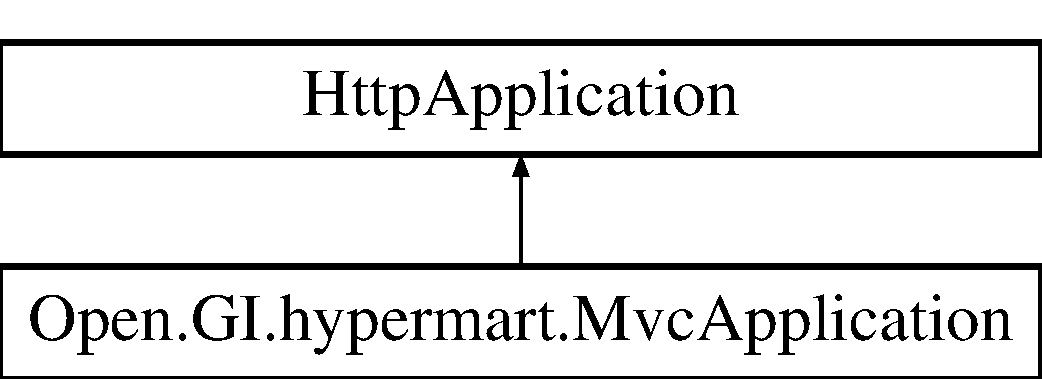
\includegraphics[height=2.000000cm]{class_open_1_1_g_i_1_1hypermart_1_1_mvc_application}
\end{center}
\end{figure}
\subsection*{Protected Member Functions}
\begin{DoxyCompactItemize}
\item 
void \textbf{ Application\+\_\+\+Start} ()
\begin{DoxyCompactList}\small\item\em A\+S\+P.\+N\+ET M\+VC Application start method \end{DoxyCompactList}\end{DoxyCompactItemize}


\subsection{Detailed Description}
Main M\+VC Application Class 

\begin{DoxySeeAlso}{See also}
System.\+Web.\+Http\+Application


\end{DoxySeeAlso}


Definition at line 17 of file Global.\+asax.\+cs.



\subsection{Member Function Documentation}
\mbox{\label{class_open_1_1_g_i_1_1hypermart_1_1_mvc_application_a8169da76cd5c9b98983e4eee8d40ce4e}} 
\index{Open\+::\+G\+I\+::hypermart\+::\+Mvc\+Application@{Open\+::\+G\+I\+::hypermart\+::\+Mvc\+Application}!Application\+\_\+\+Start@{Application\+\_\+\+Start}}
\index{Application\+\_\+\+Start@{Application\+\_\+\+Start}!Open\+::\+G\+I\+::hypermart\+::\+Mvc\+Application@{Open\+::\+G\+I\+::hypermart\+::\+Mvc\+Application}}
\subsubsection{Application\+\_\+\+Start()}
{\footnotesize\ttfamily void Open.\+G\+I.\+hypermart.\+Mvc\+Application.\+Application\+\_\+\+Start (\begin{DoxyParamCaption}{ }\end{DoxyParamCaption})\hspace{0.3cm}{\ttfamily [protected]}}



A\+S\+P.\+N\+ET M\+VC Application start method 



Definition at line 22 of file Global.\+asax.\+cs.



The documentation for this class was generated from the following file\+:\begin{DoxyCompactItemize}
\item 
C\+:/\+Projects/\+App-\/\+Utility-\/\+Store/\+Open.\+G\+I.\+hypermart/\textbf{ Global.\+asax.\+cs}\end{DoxyCompactItemize}

\hypertarget{class_open_1_1_g_i_1_1hypermart_1_1_controllers_1_1_nuget_controller}{}\section{Open.\+G\+I.\+hypermart.\+Controllers.\+Nuget\+Controller Class Reference}
\label{class_open_1_1_g_i_1_1hypermart_1_1_controllers_1_1_nuget_controller}\index{Open.\+G\+I.\+hypermart.\+Controllers.\+Nuget\+Controller@{Open.\+G\+I.\+hypermart.\+Controllers.\+Nuget\+Controller}}


An attempt to create a Nuget controller (phase 2)  


Inheritance diagram for Open.\+G\+I.\+hypermart.\+Controllers.\+Nuget\+Controller\+:\begin{figure}[H]
\begin{center}
\leavevmode
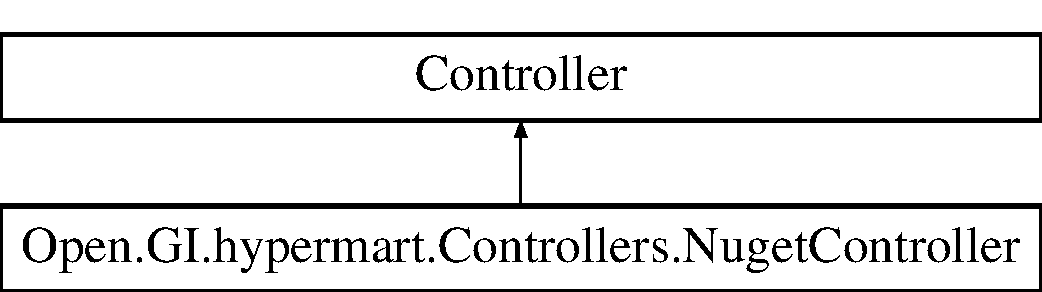
\includegraphics[height=2.000000cm]{class_open_1_1_g_i_1_1hypermart_1_1_controllers_1_1_nuget_controller}
\end{center}
\end{figure}
\subsection*{Public Member Functions}
\begin{DoxyCompactItemize}
\item 
Action\+Result \hyperlink{class_open_1_1_g_i_1_1hypermart_1_1_controllers_1_1_nuget_controller_a4512f0f0edfb480430dea27f009d37a6}{Index} ()
\begin{DoxyCompactList}\small\item\em Indexes this instance. \end{DoxyCompactList}\item 
\hyperlink{class_open_1_1_g_i_1_1hypermart_1_1_helpers_1_1_atom_action_result}{Atom\+Action\+Result} \hyperlink{class_open_1_1_g_i_1_1hypermart_1_1_controllers_1_1_nuget_controller_a8b2f4aa532a73eaacab1efcfd3fed054}{Packages} ()
\begin{DoxyCompactList}\small\item\em Packageses this instance. \end{DoxyCompactList}\end{DoxyCompactItemize}


\subsection{Detailed Description}
An attempt to create a Nuget controller (phase 2) 

\begin{DoxySeeAlso}{See also}
System.\+Web.\+Mvc.\+Controller


\end{DoxySeeAlso}


Definition at line 15 of file Nuget\+Controller.\+cs.



\subsection{Member Function Documentation}
\hypertarget{class_open_1_1_g_i_1_1hypermart_1_1_controllers_1_1_nuget_controller_a4512f0f0edfb480430dea27f009d37a6}{}\index{Open\+::\+G\+I\+::hypermart\+::\+Controllers\+::\+Nuget\+Controller@{Open\+::\+G\+I\+::hypermart\+::\+Controllers\+::\+Nuget\+Controller}!Index@{Index}}
\index{Index@{Index}!Open\+::\+G\+I\+::hypermart\+::\+Controllers\+::\+Nuget\+Controller@{Open\+::\+G\+I\+::hypermart\+::\+Controllers\+::\+Nuget\+Controller}}
\subsubsection[{Index()}]{\setlength{\rightskip}{0pt plus 5cm}Action\+Result Open.\+G\+I.\+hypermart.\+Controllers.\+Nuget\+Controller.\+Index (
\begin{DoxyParamCaption}
{}
\end{DoxyParamCaption}
)}\label{class_open_1_1_g_i_1_1hypermart_1_1_controllers_1_1_nuget_controller_a4512f0f0edfb480430dea27f009d37a6}


Indexes this instance. 

\begin{DoxyReturn}{Returns}

\end{DoxyReturn}


Definition at line 22 of file Nuget\+Controller.\+cs.

\hypertarget{class_open_1_1_g_i_1_1hypermart_1_1_controllers_1_1_nuget_controller_a8b2f4aa532a73eaacab1efcfd3fed054}{}\index{Open\+::\+G\+I\+::hypermart\+::\+Controllers\+::\+Nuget\+Controller@{Open\+::\+G\+I\+::hypermart\+::\+Controllers\+::\+Nuget\+Controller}!Packages@{Packages}}
\index{Packages@{Packages}!Open\+::\+G\+I\+::hypermart\+::\+Controllers\+::\+Nuget\+Controller@{Open\+::\+G\+I\+::hypermart\+::\+Controllers\+::\+Nuget\+Controller}}
\subsubsection[{Packages()}]{\setlength{\rightskip}{0pt plus 5cm}{\bf Atom\+Action\+Result} Open.\+G\+I.\+hypermart.\+Controllers.\+Nuget\+Controller.\+Packages (
\begin{DoxyParamCaption}
{}
\end{DoxyParamCaption}
)}\label{class_open_1_1_g_i_1_1hypermart_1_1_controllers_1_1_nuget_controller_a8b2f4aa532a73eaacab1efcfd3fed054}


Packageses this instance. 

\begin{DoxyReturn}{Returns}

\end{DoxyReturn}


Definition at line 31 of file Nuget\+Controller.\+cs.



The documentation for this class was generated from the following file\+:\begin{DoxyCompactItemize}
\item 
C\+:/\+Projects/\+App-\/\+Utility-\/\+Store/\+Open.\+G\+I.\+hypermart/\+Controllers/\hyperlink{_nuget_controller_8cs}{Nuget\+Controller.\+cs}\end{DoxyCompactItemize}

\hypertarget{class_open_1_1_g_i_1_1hypermart_1_1_areas_1_1_help_page_1_1_object_generator}{}\section{Open.\+G\+I.\+hypermart.\+Areas.\+Help\+Page.\+Object\+Generator Class Reference}
\label{class_open_1_1_g_i_1_1hypermart_1_1_areas_1_1_help_page_1_1_object_generator}\index{Open.\+G\+I.\+hypermart.\+Areas.\+Help\+Page.\+Object\+Generator@{Open.\+G\+I.\+hypermart.\+Areas.\+Help\+Page.\+Object\+Generator}}


This class will create an object of a given type and populate it with sample data.  


\subsection*{Public Member Functions}
\begin{DoxyCompactItemize}
\item 
object \hyperlink{class_open_1_1_g_i_1_1hypermart_1_1_areas_1_1_help_page_1_1_object_generator_a118924d1ff5f565e6e9c2893d36f35d2}{Generate\+Object} (Type type)
\begin{DoxyCompactList}\small\item\em Generates an object for a given type. The type needs to be public, have a public default constructor and settable public properties/fields. Currently it supports the following types\+: Simple types\+: int, string, Enum, Date\+Time, Uri, etc. Complex types\+: P\+O\+C\+O types. Nullables\+: Nullable$<$\+T$>$. Arrays\+: arrays of simple types or complex types. Key value pairs\+: Key\+Value\+Pair$<$\+T\+Key,\+T\+Value$>$ Tuples\+: Tuple$<$\+T1$>$, Tuple$<$\+T1,\+T2$>$, etc Dictionaries\+: I\+Dictionary$<$\+T\+Key,\+T\+Value$>$ or anything deriving from I\+Dictionary$<$\+T\+Key,\+T\+Value$>$. Collections\+: I\+List$<$\+T$>$, I\+Enumerable$<$\+T$>$, I\+Collection$<$\+T$>$, I\+List, I\+Enumerable, I\+Collection or anything deriving from I\+Collection$<$\+T$>$ or I\+List. Queryables\+: I\+Queryable, I\+Queryable$<$\+T$>$. \end{DoxyCompactList}\end{DoxyCompactItemize}


\subsection{Detailed Description}
This class will create an object of a given type and populate it with sample data. 



Definition at line 14 of file Object\+Generator.\+cs.



\subsection{Member Function Documentation}
\hypertarget{class_open_1_1_g_i_1_1hypermart_1_1_areas_1_1_help_page_1_1_object_generator_a118924d1ff5f565e6e9c2893d36f35d2}{}\index{Open\+::\+G\+I\+::hypermart\+::\+Areas\+::\+Help\+Page\+::\+Object\+Generator@{Open\+::\+G\+I\+::hypermart\+::\+Areas\+::\+Help\+Page\+::\+Object\+Generator}!Generate\+Object@{Generate\+Object}}
\index{Generate\+Object@{Generate\+Object}!Open\+::\+G\+I\+::hypermart\+::\+Areas\+::\+Help\+Page\+::\+Object\+Generator@{Open\+::\+G\+I\+::hypermart\+::\+Areas\+::\+Help\+Page\+::\+Object\+Generator}}
\subsubsection[{Generate\+Object(\+Type type)}]{\setlength{\rightskip}{0pt plus 5cm}object Open.\+G\+I.\+hypermart.\+Areas.\+Help\+Page.\+Object\+Generator.\+Generate\+Object (
\begin{DoxyParamCaption}
\item[{Type}]{type}
\end{DoxyParamCaption}
)}\label{class_open_1_1_g_i_1_1hypermart_1_1_areas_1_1_help_page_1_1_object_generator_a118924d1ff5f565e6e9c2893d36f35d2}


Generates an object for a given type. The type needs to be public, have a public default constructor and settable public properties/fields. Currently it supports the following types\+: Simple types\+: int, string, Enum, Date\+Time, Uri, etc. Complex types\+: P\+O\+C\+O types. Nullables\+: Nullable$<$\+T$>$. Arrays\+: arrays of simple types or complex types. Key value pairs\+: Key\+Value\+Pair$<$\+T\+Key,\+T\+Value$>$ Tuples\+: Tuple$<$\+T1$>$, Tuple$<$\+T1,\+T2$>$, etc Dictionaries\+: I\+Dictionary$<$\+T\+Key,\+T\+Value$>$ or anything deriving from I\+Dictionary$<$\+T\+Key,\+T\+Value$>$. Collections\+: I\+List$<$\+T$>$, I\+Enumerable$<$\+T$>$, I\+Collection$<$\+T$>$, I\+List, I\+Enumerable, I\+Collection or anything deriving from I\+Collection$<$\+T$>$ or I\+List. Queryables\+: I\+Queryable, I\+Queryable$<$\+T$>$. 


\begin{DoxyParams}{Parameters}
{\em type} & The type.\\
\hline
\end{DoxyParams}
\begin{DoxyReturn}{Returns}
An object of the given type.
\end{DoxyReturn}


Definition at line 33 of file Object\+Generator.\+cs.



The documentation for this class was generated from the following file\+:\begin{DoxyCompactItemize}
\item 
C\+:/\+Projects/\+App-\/\+Utility-\/\+Store/\+Open.\+G\+I.\+hypermart/\+Areas/\+Help\+Page/\+Sample\+Generation/\hyperlink{_object_generator_8cs}{Object\+Generator.\+cs}\end{DoxyCompactItemize}

\section{Open.\+G\+I.\+hypermart.\+Areas.\+Help\+Page.\+Model\+Descriptions.\+Parameter\+Annotation Class Reference}
\label{class_open_1_1_g_i_1_1hypermart_1_1_areas_1_1_help_page_1_1_model_descriptions_1_1_parameter_annotation}\index{Open.\+G\+I.\+hypermart.\+Areas.\+Help\+Page.\+Model\+Descriptions.\+Parameter\+Annotation@{Open.\+G\+I.\+hypermart.\+Areas.\+Help\+Page.\+Model\+Descriptions.\+Parameter\+Annotation}}


 


\subsection*{Properties}
\begin{DoxyCompactItemize}
\item 
Attribute \textbf{ Annotation\+Attribute}\hspace{0.3cm}{\ttfamily  [get, set]}
\begin{DoxyCompactList}\small\item\em Gets or sets the annotation attribute. \end{DoxyCompactList}\item 
string \textbf{ Documentation}\hspace{0.3cm}{\ttfamily  [get, set]}
\begin{DoxyCompactList}\small\item\em Gets or sets the documentation. \end{DoxyCompactList}\end{DoxyCompactItemize}


\subsection{Detailed Description}




Definition at line 8 of file Parameter\+Annotation.\+cs.



\subsection{Property Documentation}
\mbox{\label{class_open_1_1_g_i_1_1hypermart_1_1_areas_1_1_help_page_1_1_model_descriptions_1_1_parameter_annotation_a53e191aedff647b1d7cd63e2bb2219e0}} 
\index{Open\+::\+G\+I\+::hypermart\+::\+Areas\+::\+Help\+Page\+::\+Model\+Descriptions\+::\+Parameter\+Annotation@{Open\+::\+G\+I\+::hypermart\+::\+Areas\+::\+Help\+Page\+::\+Model\+Descriptions\+::\+Parameter\+Annotation}!Annotation\+Attribute@{Annotation\+Attribute}}
\index{Annotation\+Attribute@{Annotation\+Attribute}!Open\+::\+G\+I\+::hypermart\+::\+Areas\+::\+Help\+Page\+::\+Model\+Descriptions\+::\+Parameter\+Annotation@{Open\+::\+G\+I\+::hypermart\+::\+Areas\+::\+Help\+Page\+::\+Model\+Descriptions\+::\+Parameter\+Annotation}}
\subsubsection{Annotation\+Attribute}
{\footnotesize\ttfamily Attribute Open.\+G\+I.\+hypermart.\+Areas.\+Help\+Page.\+Model\+Descriptions.\+Parameter\+Annotation.\+Annotation\+Attribute\hspace{0.3cm}{\ttfamily [get]}, {\ttfamily [set]}}



Gets or sets the annotation attribute. 

The annotation attribute. 

Definition at line 16 of file Parameter\+Annotation.\+cs.

\mbox{\label{class_open_1_1_g_i_1_1hypermart_1_1_areas_1_1_help_page_1_1_model_descriptions_1_1_parameter_annotation_a9bfcc6f5d41c3630187373bbf9993fa4}} 
\index{Open\+::\+G\+I\+::hypermart\+::\+Areas\+::\+Help\+Page\+::\+Model\+Descriptions\+::\+Parameter\+Annotation@{Open\+::\+G\+I\+::hypermart\+::\+Areas\+::\+Help\+Page\+::\+Model\+Descriptions\+::\+Parameter\+Annotation}!Documentation@{Documentation}}
\index{Documentation@{Documentation}!Open\+::\+G\+I\+::hypermart\+::\+Areas\+::\+Help\+Page\+::\+Model\+Descriptions\+::\+Parameter\+Annotation@{Open\+::\+G\+I\+::hypermart\+::\+Areas\+::\+Help\+Page\+::\+Model\+Descriptions\+::\+Parameter\+Annotation}}
\subsubsection{Documentation}
{\footnotesize\ttfamily string Open.\+G\+I.\+hypermart.\+Areas.\+Help\+Page.\+Model\+Descriptions.\+Parameter\+Annotation.\+Documentation\hspace{0.3cm}{\ttfamily [get]}, {\ttfamily [set]}}



Gets or sets the documentation. 

The documentation. 

Definition at line 24 of file Parameter\+Annotation.\+cs.



The documentation for this class was generated from the following file\+:\begin{DoxyCompactItemize}
\item 
C\+:/\+Projects/\+App-\/\+Utility-\/\+Store/\+Open.\+G\+I.\+hypermart/\+Areas/\+Help\+Page/\+Model\+Descriptions/\textbf{ Parameter\+Annotation.\+cs}\end{DoxyCompactItemize}

\section{Open.\+G\+I.\+hypermart.\+Areas.\+Help\+Page.\+Model\+Descriptions.\+Parameter\+Description Class Reference}
\label{class_open_1_1_g_i_1_1hypermart_1_1_areas_1_1_help_page_1_1_model_descriptions_1_1_parameter_description}\index{Open.\+G\+I.\+hypermart.\+Areas.\+Help\+Page.\+Model\+Descriptions.\+Parameter\+Description@{Open.\+G\+I.\+hypermart.\+Areas.\+Help\+Page.\+Model\+Descriptions.\+Parameter\+Description}}


 


\subsection*{Public Member Functions}
\begin{DoxyCompactItemize}
\item 
\textbf{ Parameter\+Description} ()
\begin{DoxyCompactList}\small\item\em Initializes a new instance of the \doxyref{Parameter\+Description}{p.}{class_open_1_1_g_i_1_1hypermart_1_1_areas_1_1_help_page_1_1_model_descriptions_1_1_parameter_description} class. \end{DoxyCompactList}\end{DoxyCompactItemize}
\subsection*{Properties}
\begin{DoxyCompactItemize}
\item 
Collection$<$ \textbf{ Parameter\+Annotation} $>$ \textbf{ Annotations}\hspace{0.3cm}{\ttfamily  [get]}
\begin{DoxyCompactList}\small\item\em Gets the annotations. \end{DoxyCompactList}\item 
string \textbf{ Documentation}\hspace{0.3cm}{\ttfamily  [get, set]}
\begin{DoxyCompactList}\small\item\em Gets or sets the documentation. \end{DoxyCompactList}\item 
string \textbf{ Name}\hspace{0.3cm}{\ttfamily  [get, set]}
\begin{DoxyCompactList}\small\item\em Gets or sets the name. \end{DoxyCompactList}\item 
\textbf{ Model\+Description} \textbf{ Type\+Description}\hspace{0.3cm}{\ttfamily  [get, set]}
\begin{DoxyCompactList}\small\item\em Gets or sets the type description. \end{DoxyCompactList}\end{DoxyCompactItemize}


\subsection{Detailed Description}




Definition at line 9 of file Parameter\+Description.\+cs.



\subsection{Constructor \& Destructor Documentation}
\mbox{\label{class_open_1_1_g_i_1_1hypermart_1_1_areas_1_1_help_page_1_1_model_descriptions_1_1_parameter_description_a6a431c66f4493e970ceb5477cede9744}} 
\index{Open\+::\+G\+I\+::hypermart\+::\+Areas\+::\+Help\+Page\+::\+Model\+Descriptions\+::\+Parameter\+Description@{Open\+::\+G\+I\+::hypermart\+::\+Areas\+::\+Help\+Page\+::\+Model\+Descriptions\+::\+Parameter\+Description}!Parameter\+Description@{Parameter\+Description}}
\index{Parameter\+Description@{Parameter\+Description}!Open\+::\+G\+I\+::hypermart\+::\+Areas\+::\+Help\+Page\+::\+Model\+Descriptions\+::\+Parameter\+Description@{Open\+::\+G\+I\+::hypermart\+::\+Areas\+::\+Help\+Page\+::\+Model\+Descriptions\+::\+Parameter\+Description}}
\subsubsection{Parameter\+Description()}
{\footnotesize\ttfamily Open.\+G\+I.\+hypermart.\+Areas.\+Help\+Page.\+Model\+Descriptions.\+Parameter\+Description.\+Parameter\+Description (\begin{DoxyParamCaption}{ }\end{DoxyParamCaption})}



Initializes a new instance of the \doxyref{Parameter\+Description}{p.}{class_open_1_1_g_i_1_1hypermart_1_1_areas_1_1_help_page_1_1_model_descriptions_1_1_parameter_description} class. 



Definition at line 14 of file Parameter\+Description.\+cs.



\subsection{Property Documentation}
\mbox{\label{class_open_1_1_g_i_1_1hypermart_1_1_areas_1_1_help_page_1_1_model_descriptions_1_1_parameter_description_ab64b50d81b22dc90c5d40081722ff711}} 
\index{Open\+::\+G\+I\+::hypermart\+::\+Areas\+::\+Help\+Page\+::\+Model\+Descriptions\+::\+Parameter\+Description@{Open\+::\+G\+I\+::hypermart\+::\+Areas\+::\+Help\+Page\+::\+Model\+Descriptions\+::\+Parameter\+Description}!Annotations@{Annotations}}
\index{Annotations@{Annotations}!Open\+::\+G\+I\+::hypermart\+::\+Areas\+::\+Help\+Page\+::\+Model\+Descriptions\+::\+Parameter\+Description@{Open\+::\+G\+I\+::hypermart\+::\+Areas\+::\+Help\+Page\+::\+Model\+Descriptions\+::\+Parameter\+Description}}
\subsubsection{Annotations}
{\footnotesize\ttfamily Collection$<$\textbf{ Parameter\+Annotation}$>$ Open.\+G\+I.\+hypermart.\+Areas.\+Help\+Page.\+Model\+Descriptions.\+Parameter\+Description.\+Annotations\hspace{0.3cm}{\ttfamily [get]}}



Gets the annotations. 

The annotations. 

Definition at line 25 of file Parameter\+Description.\+cs.

\mbox{\label{class_open_1_1_g_i_1_1hypermart_1_1_areas_1_1_help_page_1_1_model_descriptions_1_1_parameter_description_a14b38b56f23972d23b7fc5594b5ac15f}} 
\index{Open\+::\+G\+I\+::hypermart\+::\+Areas\+::\+Help\+Page\+::\+Model\+Descriptions\+::\+Parameter\+Description@{Open\+::\+G\+I\+::hypermart\+::\+Areas\+::\+Help\+Page\+::\+Model\+Descriptions\+::\+Parameter\+Description}!Documentation@{Documentation}}
\index{Documentation@{Documentation}!Open\+::\+G\+I\+::hypermart\+::\+Areas\+::\+Help\+Page\+::\+Model\+Descriptions\+::\+Parameter\+Description@{Open\+::\+G\+I\+::hypermart\+::\+Areas\+::\+Help\+Page\+::\+Model\+Descriptions\+::\+Parameter\+Description}}
\subsubsection{Documentation}
{\footnotesize\ttfamily string Open.\+G\+I.\+hypermart.\+Areas.\+Help\+Page.\+Model\+Descriptions.\+Parameter\+Description.\+Documentation\hspace{0.3cm}{\ttfamily [get]}, {\ttfamily [set]}}



Gets or sets the documentation. 

The documentation. 

Definition at line 33 of file Parameter\+Description.\+cs.

\mbox{\label{class_open_1_1_g_i_1_1hypermart_1_1_areas_1_1_help_page_1_1_model_descriptions_1_1_parameter_description_a213cc3debc198eb331e57e38ecdca4ed}} 
\index{Open\+::\+G\+I\+::hypermart\+::\+Areas\+::\+Help\+Page\+::\+Model\+Descriptions\+::\+Parameter\+Description@{Open\+::\+G\+I\+::hypermart\+::\+Areas\+::\+Help\+Page\+::\+Model\+Descriptions\+::\+Parameter\+Description}!Name@{Name}}
\index{Name@{Name}!Open\+::\+G\+I\+::hypermart\+::\+Areas\+::\+Help\+Page\+::\+Model\+Descriptions\+::\+Parameter\+Description@{Open\+::\+G\+I\+::hypermart\+::\+Areas\+::\+Help\+Page\+::\+Model\+Descriptions\+::\+Parameter\+Description}}
\subsubsection{Name}
{\footnotesize\ttfamily string Open.\+G\+I.\+hypermart.\+Areas.\+Help\+Page.\+Model\+Descriptions.\+Parameter\+Description.\+Name\hspace{0.3cm}{\ttfamily [get]}, {\ttfamily [set]}}



Gets or sets the name. 

The name. 

Definition at line 41 of file Parameter\+Description.\+cs.

\mbox{\label{class_open_1_1_g_i_1_1hypermart_1_1_areas_1_1_help_page_1_1_model_descriptions_1_1_parameter_description_a175a097aa553ad65ae87f136df0e24e7}} 
\index{Open\+::\+G\+I\+::hypermart\+::\+Areas\+::\+Help\+Page\+::\+Model\+Descriptions\+::\+Parameter\+Description@{Open\+::\+G\+I\+::hypermart\+::\+Areas\+::\+Help\+Page\+::\+Model\+Descriptions\+::\+Parameter\+Description}!Type\+Description@{Type\+Description}}
\index{Type\+Description@{Type\+Description}!Open\+::\+G\+I\+::hypermart\+::\+Areas\+::\+Help\+Page\+::\+Model\+Descriptions\+::\+Parameter\+Description@{Open\+::\+G\+I\+::hypermart\+::\+Areas\+::\+Help\+Page\+::\+Model\+Descriptions\+::\+Parameter\+Description}}
\subsubsection{Type\+Description}
{\footnotesize\ttfamily \textbf{ Model\+Description} Open.\+G\+I.\+hypermart.\+Areas.\+Help\+Page.\+Model\+Descriptions.\+Parameter\+Description.\+Type\+Description\hspace{0.3cm}{\ttfamily [get]}, {\ttfamily [set]}}



Gets or sets the type description. 

The type description. 

Definition at line 49 of file Parameter\+Description.\+cs.



The documentation for this class was generated from the following file\+:\begin{DoxyCompactItemize}
\item 
C\+:/\+Projects/\+App-\/\+Utility-\/\+Store/\+Open.\+G\+I.\+hypermart/\+Areas/\+Help\+Page/\+Model\+Descriptions/\textbf{ Parameter\+Description.\+cs}\end{DoxyCompactItemize}

\section{Open.\+G\+I.\+hypermart.\+Models.\+Platform Class Reference}
\label{class_open_1_1_g_i_1_1hypermart_1_1_models_1_1_platform}\index{Open.\+G\+I.\+hypermart.\+Models.\+Platform@{Open.\+G\+I.\+hypermart.\+Models.\+Platform}}


Model Class for platform.  


\subsection*{Public Member Functions}
\begin{DoxyCompactItemize}
\item 
\textbf{ Platform} ()
\begin{DoxyCompactList}\small\item\em Initializes a new instance of the \doxyref{Platform}{p.}{class_open_1_1_g_i_1_1hypermart_1_1_models_1_1_platform} class. \end{DoxyCompactList}\item 
\textbf{ Platform} ()
\end{DoxyCompactItemize}
\subsection*{Properties}
\begin{DoxyCompactItemize}
\item 
string \textbf{ ID}\hspace{0.3cm}{\ttfamily  [get, set]}
\begin{DoxyCompactList}\small\item\em Gets or sets the identifier. \end{DoxyCompactList}\item 
string \textbf{ Platform1}\hspace{0.3cm}{\ttfamily  [get, set]}
\begin{DoxyCompactList}\small\item\em Gets or sets the platform1. \end{DoxyCompactList}\item 
virtual I\+Collection$<$ \textbf{ File} $>$ \textbf{ Files}\hspace{0.3cm}{\ttfamily  [get, set]}
\begin{DoxyCompactList}\small\item\em Gets or sets the files. \end{DoxyCompactList}\item 
virtual I\+Collection$<$ \textbf{ File\+Platform} $>$ \textbf{ File\+Platforms}\hspace{0.3cm}{\ttfamily  [get, set]}
\end{DoxyCompactItemize}


\subsection{Detailed Description}
Model Class for platform. 



Definition at line 12 of file Platform.\+cs.



\subsection{Constructor \& Destructor Documentation}
\mbox{\label{class_open_1_1_g_i_1_1hypermart_1_1_models_1_1_platform_a6c806705f4dc1171773096a5249a1563}} 
\index{Open\+::\+G\+I\+::hypermart\+::\+Models\+::\+Platform@{Open\+::\+G\+I\+::hypermart\+::\+Models\+::\+Platform}!Platform@{Platform}}
\index{Platform@{Platform}!Open\+::\+G\+I\+::hypermart\+::\+Models\+::\+Platform@{Open\+::\+G\+I\+::hypermart\+::\+Models\+::\+Platform}}
\subsubsection{Platform()\hspace{0.1cm}{\footnotesize\ttfamily [1/2]}}
{\footnotesize\ttfamily Open.\+G\+I.\+hypermart.\+Models.\+Platform.\+Platform (\begin{DoxyParamCaption}{ }\end{DoxyParamCaption})}



Initializes a new instance of the \doxyref{Platform}{p.}{class_open_1_1_g_i_1_1hypermart_1_1_models_1_1_platform} class. 



Definition at line 18 of file Platform.\+cs.

\mbox{\label{class_open_1_1_g_i_1_1hypermart_1_1_models_1_1_platform_a6c806705f4dc1171773096a5249a1563}} 
\index{Open\+::\+G\+I\+::hypermart\+::\+Models\+::\+Platform@{Open\+::\+G\+I\+::hypermart\+::\+Models\+::\+Platform}!Platform@{Platform}}
\index{Platform@{Platform}!Open\+::\+G\+I\+::hypermart\+::\+Models\+::\+Platform@{Open\+::\+G\+I\+::hypermart\+::\+Models\+::\+Platform}}
\subsubsection{Platform()\hspace{0.1cm}{\footnotesize\ttfamily [2/2]}}
{\footnotesize\ttfamily Open.\+G\+I.\+hypermart.\+Models.\+Platform.\+Platform (\begin{DoxyParamCaption}{ }\end{DoxyParamCaption})}



Definition at line 18 of file Platform.\+cs.



\subsection{Property Documentation}
\mbox{\label{class_open_1_1_g_i_1_1hypermart_1_1_models_1_1_platform_ac358f8b1b556f6d99fb47fdb29de7202}} 
\index{Open\+::\+G\+I\+::hypermart\+::\+Models\+::\+Platform@{Open\+::\+G\+I\+::hypermart\+::\+Models\+::\+Platform}!File\+Platforms@{File\+Platforms}}
\index{File\+Platforms@{File\+Platforms}!Open\+::\+G\+I\+::hypermart\+::\+Models\+::\+Platform@{Open\+::\+G\+I\+::hypermart\+::\+Models\+::\+Platform}}
\subsubsection{File\+Platforms}
{\footnotesize\ttfamily virtual I\+Collection$<$\textbf{ File\+Platform}$>$ Open.\+G\+I.\+hypermart.\+Models.\+Platform.\+File\+Platforms\hspace{0.3cm}{\ttfamily [get]}, {\ttfamily [set]}}



Definition at line 27 of file Platform.\+cs.

\mbox{\label{class_open_1_1_g_i_1_1hypermart_1_1_models_1_1_platform_a984a31b30ada1f33acef9099c09d9ca0}} 
\index{Open\+::\+G\+I\+::hypermart\+::\+Models\+::\+Platform@{Open\+::\+G\+I\+::hypermart\+::\+Models\+::\+Platform}!Files@{Files}}
\index{Files@{Files}!Open\+::\+G\+I\+::hypermart\+::\+Models\+::\+Platform@{Open\+::\+G\+I\+::hypermart\+::\+Models\+::\+Platform}}
\subsubsection{Files}
{\footnotesize\ttfamily virtual I\+Collection$<$\textbf{ File}$>$ Open.\+G\+I.\+hypermart.\+Models.\+Platform.\+Files\hspace{0.3cm}{\ttfamily [get]}, {\ttfamily [set]}}



Gets or sets the files. 

The files. 

Definition at line 47 of file Platform.\+cs.

\mbox{\label{class_open_1_1_g_i_1_1hypermart_1_1_models_1_1_platform_ae11ad27de467131d539e35f598ff3051}} 
\index{Open\+::\+G\+I\+::hypermart\+::\+Models\+::\+Platform@{Open\+::\+G\+I\+::hypermart\+::\+Models\+::\+Platform}!ID@{ID}}
\index{ID@{ID}!Open\+::\+G\+I\+::hypermart\+::\+Models\+::\+Platform@{Open\+::\+G\+I\+::hypermart\+::\+Models\+::\+Platform}}
\subsubsection{ID}
{\footnotesize\ttfamily string Open.\+G\+I.\+hypermart.\+Models.\+Platform.\+ID\hspace{0.3cm}{\ttfamily [get]}, {\ttfamily [set]}}



Gets or sets the identifier. 

The identifier. 

Definition at line 30 of file Platform.\+cs.

\mbox{\label{class_open_1_1_g_i_1_1hypermart_1_1_models_1_1_platform_aa93619cbb18655b2425f416df0f194c6}} 
\index{Open\+::\+G\+I\+::hypermart\+::\+Models\+::\+Platform@{Open\+::\+G\+I\+::hypermart\+::\+Models\+::\+Platform}!Platform1@{Platform1}}
\index{Platform1@{Platform1}!Open\+::\+G\+I\+::hypermart\+::\+Models\+::\+Platform@{Open\+::\+G\+I\+::hypermart\+::\+Models\+::\+Platform}}
\subsubsection{Platform1}
{\footnotesize\ttfamily string Open.\+G\+I.\+hypermart.\+Models.\+Platform.\+Platform1\hspace{0.3cm}{\ttfamily [get]}, {\ttfamily [set]}}



Gets or sets the platform1. 

The platform1. 

Definition at line 38 of file Platform.\+cs.



The documentation for this class was generated from the following file\+:\begin{DoxyCompactItemize}
\item 
C\+:/\+Projects/\+App-\/\+Utility-\/\+Store/\+Open.\+G\+I.\+hypermart/\+Models/\textbf{ Platform.\+cs}\end{DoxyCompactItemize}

\hypertarget{class_open_1_1_g_i_1_1hypermart_1_1_models_1_1_product}{}\section{Open.\+G\+I.\+hypermart.\+Models.\+Product Class Reference}
\label{class_open_1_1_g_i_1_1hypermart_1_1_models_1_1_product}\index{Open.\+G\+I.\+hypermart.\+Models.\+Product@{Open.\+G\+I.\+hypermart.\+Models.\+Product}}


\hyperlink{class_open_1_1_g_i_1_1hypermart_1_1_models_1_1_product}{Product} Model Class  


\subsection*{Public Member Functions}
\begin{DoxyCompactItemize}
\item 
\hyperlink{class_open_1_1_g_i_1_1hypermart_1_1_models_1_1_product_a6e3b824c07f190baa506f9c73da63e62}{Product} ()
\begin{DoxyCompactList}\small\item\em Initializes a new instance of the \hyperlink{class_open_1_1_g_i_1_1hypermart_1_1_models_1_1_product}{Product} class. \end{DoxyCompactList}\item 
\hyperlink{class_open_1_1_g_i_1_1hypermart_1_1_models_1_1_product_a6e3b824c07f190baa506f9c73da63e62}{Product} ()
\end{DoxyCompactItemize}
\subsection*{Properties}
\begin{DoxyCompactItemize}
\item 
int \hyperlink{class_open_1_1_g_i_1_1hypermart_1_1_models_1_1_product_a4fedd3f62a9c36939c6e45ea2e8cd011}{I\+D}\hspace{0.3cm}{\ttfamily  \mbox{[}get, set\mbox{]}}
\begin{DoxyCompactList}\small\item\em Gets or sets the identifier. \end{DoxyCompactList}\item 
string \hyperlink{class_open_1_1_g_i_1_1hypermart_1_1_models_1_1_product_a877241a61c423e91b6b630df5ca811d0}{Title}\hspace{0.3cm}{\ttfamily  \mbox{[}get, set\mbox{]}}
\begin{DoxyCompactList}\small\item\em Gets or sets the title. \end{DoxyCompactList}\item 
string \hyperlink{class_open_1_1_g_i_1_1hypermart_1_1_models_1_1_product_a8d7cb8cd22f77fa66f06726400b1381e}{Description}\hspace{0.3cm}{\ttfamily  \mbox{[}get, set\mbox{]}}
\begin{DoxyCompactList}\small\item\em Gets or sets the description. \end{DoxyCompactList}\item 
string \hyperlink{class_open_1_1_g_i_1_1hypermart_1_1_models_1_1_product_ad0233eb35ac4048277a4eafde6432c43}{Tagline}\hspace{0.3cm}{\ttfamily  \mbox{[}get, set\mbox{]}}
\begin{DoxyCompactList}\small\item\em Gets or sets the tagline. \end{DoxyCompactList}\item 
string \hyperlink{class_open_1_1_g_i_1_1hypermart_1_1_models_1_1_product_a646bc5e183ba8d87c06d290398e6bee6}{Lead}\hspace{0.3cm}{\ttfamily  \mbox{[}get, set\mbox{]}}
\begin{DoxyCompactList}\small\item\em Gets or sets the lead. \end{DoxyCompactList}\item 
string \hyperlink{class_open_1_1_g_i_1_1hypermart_1_1_models_1_1_product_ab5fd5620220d0e68053208859137a6cb}{Source\+Code}\hspace{0.3cm}{\ttfamily  \mbox{[}get, set\mbox{]}}
\begin{DoxyCompactList}\small\item\em Gets or sets the source code location for the project. \end{DoxyCompactList}\item 
virtual I\+Collection$<$ string $>$ \hyperlink{class_open_1_1_g_i_1_1hypermart_1_1_models_1_1_product_af39b6e12bee2265db7bbca5ecbeb116c}{Maintainers}\hspace{0.3cm}{\ttfamily  \mbox{[}get, set\mbox{]}}
\begin{DoxyCompactList}\small\item\em Gets or sets the maintainers. \end{DoxyCompactList}\item 
virtual I\+Collection$<$ \hyperlink{class_open_1_1_g_i_1_1hypermart_1_1_models_1_1_file}{File} $>$ \hyperlink{class_open_1_1_g_i_1_1hypermart_1_1_models_1_1_product_a8632e80d5f05c8818c289b3924137c13}{Files}\hspace{0.3cm}{\ttfamily  \mbox{[}get, set\mbox{]}}
\begin{DoxyCompactList}\small\item\em Gets or sets the files. \end{DoxyCompactList}\item 
virtual I\+Collection$<$ \hyperlink{class_open_1_1_g_i_1_1hypermart_1_1_models_1_1_screenshot}{Screenshot} $>$ \hyperlink{class_open_1_1_g_i_1_1hypermart_1_1_models_1_1_product_a5fae1aafb8f9a3af27ce369d5d053df1}{Screenshots}\hspace{0.3cm}{\ttfamily  \mbox{[}get, set\mbox{]}}
\begin{DoxyCompactList}\small\item\em Gets or sets the screenshots. \end{DoxyCompactList}\end{DoxyCompactItemize}


\subsection{Detailed Description}
\hyperlink{class_open_1_1_g_i_1_1hypermart_1_1_models_1_1_product}{Product} Model Class 



Definition at line 12 of file Product.\+cs.



\subsection{Constructor \& Destructor Documentation}
\hypertarget{class_open_1_1_g_i_1_1hypermart_1_1_models_1_1_product_a6e3b824c07f190baa506f9c73da63e62}{}\index{Open\+::\+G\+I\+::hypermart\+::\+Models\+::\+Product@{Open\+::\+G\+I\+::hypermart\+::\+Models\+::\+Product}!Product@{Product}}
\index{Product@{Product}!Open\+::\+G\+I\+::hypermart\+::\+Models\+::\+Product@{Open\+::\+G\+I\+::hypermart\+::\+Models\+::\+Product}}
\subsubsection[{Product()}]{\setlength{\rightskip}{0pt plus 5cm}Open.\+G\+I.\+hypermart.\+Models.\+Product.\+Product (
\begin{DoxyParamCaption}
{}
\end{DoxyParamCaption}
)}\label{class_open_1_1_g_i_1_1hypermart_1_1_models_1_1_product_a6e3b824c07f190baa506f9c73da63e62}


Initializes a new instance of the \hyperlink{class_open_1_1_g_i_1_1hypermart_1_1_models_1_1_product}{Product} class. 



Definition at line 18 of file Product.\+cs.

\hypertarget{class_open_1_1_g_i_1_1hypermart_1_1_models_1_1_product_a6e3b824c07f190baa506f9c73da63e62}{}\index{Open\+::\+G\+I\+::hypermart\+::\+Models\+::\+Product@{Open\+::\+G\+I\+::hypermart\+::\+Models\+::\+Product}!Product@{Product}}
\index{Product@{Product}!Open\+::\+G\+I\+::hypermart\+::\+Models\+::\+Product@{Open\+::\+G\+I\+::hypermart\+::\+Models\+::\+Product}}
\subsubsection[{Product()}]{\setlength{\rightskip}{0pt plus 5cm}Open.\+G\+I.\+hypermart.\+Models.\+Product.\+Product (
\begin{DoxyParamCaption}
{}
\end{DoxyParamCaption}
)}\label{class_open_1_1_g_i_1_1hypermart_1_1_models_1_1_product_a6e3b824c07f190baa506f9c73da63e62}


Definition at line 18 of file Product.\+cs.



\subsection{Property Documentation}
\hypertarget{class_open_1_1_g_i_1_1hypermart_1_1_models_1_1_product_a8d7cb8cd22f77fa66f06726400b1381e}{}\index{Open\+::\+G\+I\+::hypermart\+::\+Models\+::\+Product@{Open\+::\+G\+I\+::hypermart\+::\+Models\+::\+Product}!Description@{Description}}
\index{Description@{Description}!Open\+::\+G\+I\+::hypermart\+::\+Models\+::\+Product@{Open\+::\+G\+I\+::hypermart\+::\+Models\+::\+Product}}
\subsubsection[{Description}]{\setlength{\rightskip}{0pt plus 5cm}string Open.\+G\+I.\+hypermart.\+Models.\+Product.\+Description\hspace{0.3cm}{\ttfamily [get]}, {\ttfamily [set]}}\label{class_open_1_1_g_i_1_1hypermart_1_1_models_1_1_product_a8d7cb8cd22f77fa66f06726400b1381e}


Gets or sets the description. 

The description. 

Definition at line 46 of file Product.\+cs.

\hypertarget{class_open_1_1_g_i_1_1hypermart_1_1_models_1_1_product_a8632e80d5f05c8818c289b3924137c13}{}\index{Open\+::\+G\+I\+::hypermart\+::\+Models\+::\+Product@{Open\+::\+G\+I\+::hypermart\+::\+Models\+::\+Product}!Files@{Files}}
\index{Files@{Files}!Open\+::\+G\+I\+::hypermart\+::\+Models\+::\+Product@{Open\+::\+G\+I\+::hypermart\+::\+Models\+::\+Product}}
\subsubsection[{Files}]{\setlength{\rightskip}{0pt plus 5cm}I\+Collection$<$ {\bf File} $>$ Open.\+G\+I.\+hypermart.\+Models.\+Product.\+Files\hspace{0.3cm}{\ttfamily [get]}, {\ttfamily [set]}}\label{class_open_1_1_g_i_1_1hypermart_1_1_models_1_1_product_a8632e80d5f05c8818c289b3924137c13}


Gets or sets the files. 

The files. 

Definition at line 90 of file Product.\+cs.

\hypertarget{class_open_1_1_g_i_1_1hypermart_1_1_models_1_1_product_a4fedd3f62a9c36939c6e45ea2e8cd011}{}\index{Open\+::\+G\+I\+::hypermart\+::\+Models\+::\+Product@{Open\+::\+G\+I\+::hypermart\+::\+Models\+::\+Product}!I\+D@{I\+D}}
\index{I\+D@{I\+D}!Open\+::\+G\+I\+::hypermart\+::\+Models\+::\+Product@{Open\+::\+G\+I\+::hypermart\+::\+Models\+::\+Product}}
\subsubsection[{I\+D}]{\setlength{\rightskip}{0pt plus 5cm}int Open.\+G\+I.\+hypermart.\+Models.\+Product.\+I\+D\hspace{0.3cm}{\ttfamily [get]}, {\ttfamily [set]}}\label{class_open_1_1_g_i_1_1hypermart_1_1_models_1_1_product_a4fedd3f62a9c36939c6e45ea2e8cd011}


Gets or sets the identifier. 

The identifier. 

Definition at line 30 of file Product.\+cs.

\hypertarget{class_open_1_1_g_i_1_1hypermart_1_1_models_1_1_product_a646bc5e183ba8d87c06d290398e6bee6}{}\index{Open\+::\+G\+I\+::hypermart\+::\+Models\+::\+Product@{Open\+::\+G\+I\+::hypermart\+::\+Models\+::\+Product}!Lead@{Lead}}
\index{Lead@{Lead}!Open\+::\+G\+I\+::hypermart\+::\+Models\+::\+Product@{Open\+::\+G\+I\+::hypermart\+::\+Models\+::\+Product}}
\subsubsection[{Lead}]{\setlength{\rightskip}{0pt plus 5cm}string Open.\+G\+I.\+hypermart.\+Models.\+Product.\+Lead\hspace{0.3cm}{\ttfamily [get]}, {\ttfamily [set]}}\label{class_open_1_1_g_i_1_1hypermart_1_1_models_1_1_product_a646bc5e183ba8d87c06d290398e6bee6}


Gets or sets the lead. 

The lead. 

Definition at line 63 of file Product.\+cs.

\hypertarget{class_open_1_1_g_i_1_1hypermart_1_1_models_1_1_product_af39b6e12bee2265db7bbca5ecbeb116c}{}\index{Open\+::\+G\+I\+::hypermart\+::\+Models\+::\+Product@{Open\+::\+G\+I\+::hypermart\+::\+Models\+::\+Product}!Maintainers@{Maintainers}}
\index{Maintainers@{Maintainers}!Open\+::\+G\+I\+::hypermart\+::\+Models\+::\+Product@{Open\+::\+G\+I\+::hypermart\+::\+Models\+::\+Product}}
\subsubsection[{Maintainers}]{\setlength{\rightskip}{0pt plus 5cm}virtual I\+Collection$<$string$>$ Open.\+G\+I.\+hypermart.\+Models.\+Product.\+Maintainers\hspace{0.3cm}{\ttfamily [get]}, {\ttfamily [set]}}\label{class_open_1_1_g_i_1_1hypermart_1_1_models_1_1_product_af39b6e12bee2265db7bbca5ecbeb116c}


Gets or sets the maintainers. 

The maintainers. 

Definition at line 80 of file Product.\+cs.

\hypertarget{class_open_1_1_g_i_1_1hypermart_1_1_models_1_1_product_a5fae1aafb8f9a3af27ce369d5d053df1}{}\index{Open\+::\+G\+I\+::hypermart\+::\+Models\+::\+Product@{Open\+::\+G\+I\+::hypermart\+::\+Models\+::\+Product}!Screenshots@{Screenshots}}
\index{Screenshots@{Screenshots}!Open\+::\+G\+I\+::hypermart\+::\+Models\+::\+Product@{Open\+::\+G\+I\+::hypermart\+::\+Models\+::\+Product}}
\subsubsection[{Screenshots}]{\setlength{\rightskip}{0pt plus 5cm}I\+Collection$<$ {\bf Screenshot} $>$ Open.\+G\+I.\+hypermart.\+Models.\+Product.\+Screenshots\hspace{0.3cm}{\ttfamily [get]}, {\ttfamily [set]}}\label{class_open_1_1_g_i_1_1hypermart_1_1_models_1_1_product_a5fae1aafb8f9a3af27ce369d5d053df1}


Gets or sets the screenshots. 

The screenshots. 

Definition at line 99 of file Product.\+cs.

\hypertarget{class_open_1_1_g_i_1_1hypermart_1_1_models_1_1_product_ab5fd5620220d0e68053208859137a6cb}{}\index{Open\+::\+G\+I\+::hypermart\+::\+Models\+::\+Product@{Open\+::\+G\+I\+::hypermart\+::\+Models\+::\+Product}!Source\+Code@{Source\+Code}}
\index{Source\+Code@{Source\+Code}!Open\+::\+G\+I\+::hypermart\+::\+Models\+::\+Product@{Open\+::\+G\+I\+::hypermart\+::\+Models\+::\+Product}}
\subsubsection[{Source\+Code}]{\setlength{\rightskip}{0pt plus 5cm}string Open.\+G\+I.\+hypermart.\+Models.\+Product.\+Source\+Code\hspace{0.3cm}{\ttfamily [get]}, {\ttfamily [set]}}\label{class_open_1_1_g_i_1_1hypermart_1_1_models_1_1_product_ab5fd5620220d0e68053208859137a6cb}


Gets or sets the source code location for the project. 

The source code. 

Definition at line 71 of file Product.\+cs.

\hypertarget{class_open_1_1_g_i_1_1hypermart_1_1_models_1_1_product_ad0233eb35ac4048277a4eafde6432c43}{}\index{Open\+::\+G\+I\+::hypermart\+::\+Models\+::\+Product@{Open\+::\+G\+I\+::hypermart\+::\+Models\+::\+Product}!Tagline@{Tagline}}
\index{Tagline@{Tagline}!Open\+::\+G\+I\+::hypermart\+::\+Models\+::\+Product@{Open\+::\+G\+I\+::hypermart\+::\+Models\+::\+Product}}
\subsubsection[{Tagline}]{\setlength{\rightskip}{0pt plus 5cm}string Open.\+G\+I.\+hypermart.\+Models.\+Product.\+Tagline\hspace{0.3cm}{\ttfamily [get]}, {\ttfamily [set]}}\label{class_open_1_1_g_i_1_1hypermart_1_1_models_1_1_product_ad0233eb35ac4048277a4eafde6432c43}


Gets or sets the tagline. 

The tagline. 

Definition at line 54 of file Product.\+cs.

\hypertarget{class_open_1_1_g_i_1_1hypermart_1_1_models_1_1_product_a877241a61c423e91b6b630df5ca811d0}{}\index{Open\+::\+G\+I\+::hypermart\+::\+Models\+::\+Product@{Open\+::\+G\+I\+::hypermart\+::\+Models\+::\+Product}!Title@{Title}}
\index{Title@{Title}!Open\+::\+G\+I\+::hypermart\+::\+Models\+::\+Product@{Open\+::\+G\+I\+::hypermart\+::\+Models\+::\+Product}}
\subsubsection[{Title}]{\setlength{\rightskip}{0pt plus 5cm}string Open.\+G\+I.\+hypermart.\+Models.\+Product.\+Title\hspace{0.3cm}{\ttfamily [get]}, {\ttfamily [set]}}\label{class_open_1_1_g_i_1_1hypermart_1_1_models_1_1_product_a877241a61c423e91b6b630df5ca811d0}


Gets or sets the title. 

The title. 

Definition at line 38 of file Product.\+cs.



The documentation for this class was generated from the following file\+:\begin{DoxyCompactItemize}
\item 
C\+:/\+Projects/\+App-\/\+Utility-\/\+Store/\+Open.\+G\+I.\+hypermart/\+Models/\hyperlink{_models_2_product_8cs}{Product.\+cs}\end{DoxyCompactItemize}

\section{Open.\+G\+I.\+hypermart.\+Data\+Transformation\+Objects.\+Product\+D\+TO Class Reference}
\label{class_open_1_1_g_i_1_1hypermart_1_1_data_transformation_objects_1_1_product_d_t_o}\index{Open.\+G\+I.\+hypermart.\+Data\+Transformation\+Objects.\+Product\+D\+TO@{Open.\+G\+I.\+hypermart.\+Data\+Transformation\+Objects.\+Product\+D\+TO}}


 


\subsection*{Public Member Functions}
\begin{DoxyCompactItemize}
\item 
\textbf{ Product\+D\+TO} ()
\begin{DoxyCompactList}\small\item\em Initializes a new instance of the \doxyref{Product\+D\+TO}{p.}{class_open_1_1_g_i_1_1hypermart_1_1_data_transformation_objects_1_1_product_d_t_o} class. \end{DoxyCompactList}\item 
\textbf{ Product\+D\+TO} (\textbf{ Product} prod)
\begin{DoxyCompactList}\small\item\em Initializes a new instance of the \doxyref{Product\+D\+TO}{p.}{class_open_1_1_g_i_1_1hypermart_1_1_data_transformation_objects_1_1_product_d_t_o} class. \end{DoxyCompactList}\end{DoxyCompactItemize}
\subsection*{Properties}
\begin{DoxyCompactItemize}
\item 
int \textbf{ ID}\hspace{0.3cm}{\ttfamily  [get, set]}
\begin{DoxyCompactList}\small\item\em Gets or sets the identifier. \end{DoxyCompactList}\item 
string \textbf{ Title}\hspace{0.3cm}{\ttfamily  [get, set]}
\begin{DoxyCompactList}\small\item\em Gets or sets the title. \end{DoxyCompactList}\item 
string \textbf{ Description}\hspace{0.3cm}{\ttfamily  [get, set]}
\begin{DoxyCompactList}\small\item\em Gets or sets the description. \end{DoxyCompactList}\item 
string \textbf{ Tagline}\hspace{0.3cm}{\ttfamily  [get, set]}
\begin{DoxyCompactList}\small\item\em Gets or sets the tagline. \end{DoxyCompactList}\item 
string \textbf{ Lead}\hspace{0.3cm}{\ttfamily  [get, set]}
\begin{DoxyCompactList}\small\item\em Gets or sets the lead. \end{DoxyCompactList}\item 
List$<$ byte[$\,$]$>$ \textbf{ Screen\+Shot}\hspace{0.3cm}{\ttfamily  [get, set]}
\begin{DoxyCompactList}\small\item\em Screen Shot \end{DoxyCompactList}\end{DoxyCompactItemize}


\subsection{Detailed Description}




Definition at line 13 of file Product\+D\+T\+O.\+cs.



\subsection{Constructor \& Destructor Documentation}
\mbox{\label{class_open_1_1_g_i_1_1hypermart_1_1_data_transformation_objects_1_1_product_d_t_o_a99130c4316beb76caa542b78f0de4e38}} 
\index{Open\+::\+G\+I\+::hypermart\+::\+Data\+Transformation\+Objects\+::\+Product\+D\+TO@{Open\+::\+G\+I\+::hypermart\+::\+Data\+Transformation\+Objects\+::\+Product\+D\+TO}!Product\+D\+TO@{Product\+D\+TO}}
\index{Product\+D\+TO@{Product\+D\+TO}!Open\+::\+G\+I\+::hypermart\+::\+Data\+Transformation\+Objects\+::\+Product\+D\+TO@{Open\+::\+G\+I\+::hypermart\+::\+Data\+Transformation\+Objects\+::\+Product\+D\+TO}}
\subsubsection{Product\+D\+T\+O()\hspace{0.1cm}{\footnotesize\ttfamily [1/2]}}
{\footnotesize\ttfamily Open.\+G\+I.\+hypermart.\+Data\+Transformation\+Objects.\+Product\+D\+T\+O.\+Product\+D\+TO (\begin{DoxyParamCaption}{ }\end{DoxyParamCaption})}



Initializes a new instance of the \doxyref{Product\+D\+TO}{p.}{class_open_1_1_g_i_1_1hypermart_1_1_data_transformation_objects_1_1_product_d_t_o} class. 



Definition at line 18 of file Product\+D\+T\+O.\+cs.

\mbox{\label{class_open_1_1_g_i_1_1hypermart_1_1_data_transformation_objects_1_1_product_d_t_o_a4deb78b33f6f3fc07ec2d4f49ada1f93}} 
\index{Open\+::\+G\+I\+::hypermart\+::\+Data\+Transformation\+Objects\+::\+Product\+D\+TO@{Open\+::\+G\+I\+::hypermart\+::\+Data\+Transformation\+Objects\+::\+Product\+D\+TO}!Product\+D\+TO@{Product\+D\+TO}}
\index{Product\+D\+TO@{Product\+D\+TO}!Open\+::\+G\+I\+::hypermart\+::\+Data\+Transformation\+Objects\+::\+Product\+D\+TO@{Open\+::\+G\+I\+::hypermart\+::\+Data\+Transformation\+Objects\+::\+Product\+D\+TO}}
\subsubsection{Product\+D\+T\+O()\hspace{0.1cm}{\footnotesize\ttfamily [2/2]}}
{\footnotesize\ttfamily Open.\+G\+I.\+hypermart.\+Data\+Transformation\+Objects.\+Product\+D\+T\+O.\+Product\+D\+TO (\begin{DoxyParamCaption}\item[{\textbf{ Product}}]{prod }\end{DoxyParamCaption})}



Initializes a new instance of the \doxyref{Product\+D\+TO}{p.}{class_open_1_1_g_i_1_1hypermart_1_1_data_transformation_objects_1_1_product_d_t_o} class. 


\begin{DoxyParams}{Parameters}
{\em prod} & The base.\\
\hline
\end{DoxyParams}


Definition at line 26 of file Product\+D\+T\+O.\+cs.



\subsection{Property Documentation}
\mbox{\label{class_open_1_1_g_i_1_1hypermart_1_1_data_transformation_objects_1_1_product_d_t_o_a1de153f9a50688af8c97932d30056fef}} 
\index{Open\+::\+G\+I\+::hypermart\+::\+Data\+Transformation\+Objects\+::\+Product\+D\+TO@{Open\+::\+G\+I\+::hypermart\+::\+Data\+Transformation\+Objects\+::\+Product\+D\+TO}!Description@{Description}}
\index{Description@{Description}!Open\+::\+G\+I\+::hypermart\+::\+Data\+Transformation\+Objects\+::\+Product\+D\+TO@{Open\+::\+G\+I\+::hypermart\+::\+Data\+Transformation\+Objects\+::\+Product\+D\+TO}}
\subsubsection{Description}
{\footnotesize\ttfamily string Open.\+G\+I.\+hypermart.\+Data\+Transformation\+Objects.\+Product\+D\+T\+O.\+Description\hspace{0.3cm}{\ttfamily [get]}, {\ttfamily [set]}}



Gets or sets the description. 

The description. 

Definition at line 62 of file Product\+D\+T\+O.\+cs.

\mbox{\label{class_open_1_1_g_i_1_1hypermart_1_1_data_transformation_objects_1_1_product_d_t_o_ab965f0f2be3b04afb1de5e8fa97cd93a}} 
\index{Open\+::\+G\+I\+::hypermart\+::\+Data\+Transformation\+Objects\+::\+Product\+D\+TO@{Open\+::\+G\+I\+::hypermart\+::\+Data\+Transformation\+Objects\+::\+Product\+D\+TO}!ID@{ID}}
\index{ID@{ID}!Open\+::\+G\+I\+::hypermart\+::\+Data\+Transformation\+Objects\+::\+Product\+D\+TO@{Open\+::\+G\+I\+::hypermart\+::\+Data\+Transformation\+Objects\+::\+Product\+D\+TO}}
\subsubsection{ID}
{\footnotesize\ttfamily int Open.\+G\+I.\+hypermart.\+Data\+Transformation\+Objects.\+Product\+D\+T\+O.\+ID\hspace{0.3cm}{\ttfamily [get]}, {\ttfamily [set]}}



Gets or sets the identifier. 

The identifier. 

Definition at line 46 of file Product\+D\+T\+O.\+cs.

\mbox{\label{class_open_1_1_g_i_1_1hypermart_1_1_data_transformation_objects_1_1_product_d_t_o_a900af3a5017cf99ef7a51c8a496289cc}} 
\index{Open\+::\+G\+I\+::hypermart\+::\+Data\+Transformation\+Objects\+::\+Product\+D\+TO@{Open\+::\+G\+I\+::hypermart\+::\+Data\+Transformation\+Objects\+::\+Product\+D\+TO}!Lead@{Lead}}
\index{Lead@{Lead}!Open\+::\+G\+I\+::hypermart\+::\+Data\+Transformation\+Objects\+::\+Product\+D\+TO@{Open\+::\+G\+I\+::hypermart\+::\+Data\+Transformation\+Objects\+::\+Product\+D\+TO}}
\subsubsection{Lead}
{\footnotesize\ttfamily string Open.\+G\+I.\+hypermart.\+Data\+Transformation\+Objects.\+Product\+D\+T\+O.\+Lead\hspace{0.3cm}{\ttfamily [get]}, {\ttfamily [set]}}



Gets or sets the lead. 

The lead. 

Definition at line 79 of file Product\+D\+T\+O.\+cs.

\mbox{\label{class_open_1_1_g_i_1_1hypermart_1_1_data_transformation_objects_1_1_product_d_t_o_ac2f998445710bc55481fe5983ed485de}} 
\index{Open\+::\+G\+I\+::hypermart\+::\+Data\+Transformation\+Objects\+::\+Product\+D\+TO@{Open\+::\+G\+I\+::hypermart\+::\+Data\+Transformation\+Objects\+::\+Product\+D\+TO}!Screen\+Shot@{Screen\+Shot}}
\index{Screen\+Shot@{Screen\+Shot}!Open\+::\+G\+I\+::hypermart\+::\+Data\+Transformation\+Objects\+::\+Product\+D\+TO@{Open\+::\+G\+I\+::hypermart\+::\+Data\+Transformation\+Objects\+::\+Product\+D\+TO}}
\subsubsection{Screen\+Shot}
{\footnotesize\ttfamily List$<$byte[$\,$]$>$ Open.\+G\+I.\+hypermart.\+Data\+Transformation\+Objects.\+Product\+D\+T\+O.\+Screen\+Shot\hspace{0.3cm}{\ttfamily [get]}, {\ttfamily [set]}}



Screen Shot 



Definition at line 84 of file Product\+D\+T\+O.\+cs.

\mbox{\label{class_open_1_1_g_i_1_1hypermart_1_1_data_transformation_objects_1_1_product_d_t_o_a7b9cf190d3a304a72287dc1c0200aa94}} 
\index{Open\+::\+G\+I\+::hypermart\+::\+Data\+Transformation\+Objects\+::\+Product\+D\+TO@{Open\+::\+G\+I\+::hypermart\+::\+Data\+Transformation\+Objects\+::\+Product\+D\+TO}!Tagline@{Tagline}}
\index{Tagline@{Tagline}!Open\+::\+G\+I\+::hypermart\+::\+Data\+Transformation\+Objects\+::\+Product\+D\+TO@{Open\+::\+G\+I\+::hypermart\+::\+Data\+Transformation\+Objects\+::\+Product\+D\+TO}}
\subsubsection{Tagline}
{\footnotesize\ttfamily string Open.\+G\+I.\+hypermart.\+Data\+Transformation\+Objects.\+Product\+D\+T\+O.\+Tagline\hspace{0.3cm}{\ttfamily [get]}, {\ttfamily [set]}}



Gets or sets the tagline. 

The tagline. 

Definition at line 70 of file Product\+D\+T\+O.\+cs.

\mbox{\label{class_open_1_1_g_i_1_1hypermart_1_1_data_transformation_objects_1_1_product_d_t_o_a6f03b28697c295061d5c914d5598efef}} 
\index{Open\+::\+G\+I\+::hypermart\+::\+Data\+Transformation\+Objects\+::\+Product\+D\+TO@{Open\+::\+G\+I\+::hypermart\+::\+Data\+Transformation\+Objects\+::\+Product\+D\+TO}!Title@{Title}}
\index{Title@{Title}!Open\+::\+G\+I\+::hypermart\+::\+Data\+Transformation\+Objects\+::\+Product\+D\+TO@{Open\+::\+G\+I\+::hypermart\+::\+Data\+Transformation\+Objects\+::\+Product\+D\+TO}}
\subsubsection{Title}
{\footnotesize\ttfamily string Open.\+G\+I.\+hypermart.\+Data\+Transformation\+Objects.\+Product\+D\+T\+O.\+Title\hspace{0.3cm}{\ttfamily [get]}, {\ttfamily [set]}}



Gets or sets the title. 

The title. 

Definition at line 54 of file Product\+D\+T\+O.\+cs.



The documentation for this class was generated from the following file\+:\begin{DoxyCompactItemize}
\item 
C\+:/\+Projects/\+App-\/\+Utility-\/\+Store/\+Open.\+G\+I.\+hypermart/\+Docs/\+Data\+Transformation\+Objects/\textbf{ Product\+D\+T\+O.\+cs}\end{DoxyCompactItemize}

\section{Open.\+G\+I.\+hypermart.\+Controllers.\+Products\+Controller Class Reference}
\label{class_open_1_1_g_i_1_1hypermart_1_1_controllers_1_1_products_controller}\index{Open.\+G\+I.\+hypermart.\+Controllers.\+Products\+Controller@{Open.\+G\+I.\+hypermart.\+Controllers.\+Products\+Controller}}


 


Inheritance diagram for Open.\+G\+I.\+hypermart.\+Controllers.\+Products\+Controller\+:\begin{figure}[H]
\begin{center}
\leavevmode
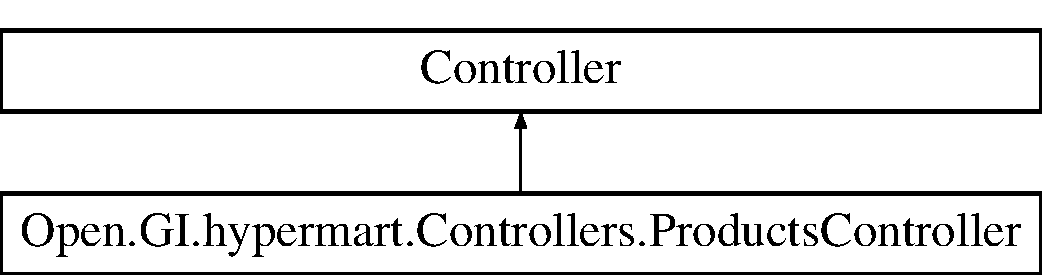
\includegraphics[height=2.000000cm]{class_open_1_1_g_i_1_1hypermart_1_1_controllers_1_1_products_controller}
\end{center}
\end{figure}
\subsection*{Public Member Functions}
\begin{DoxyCompactItemize}
\item 
\textbf{ Products\+Controller} ()
\begin{DoxyCompactList}\small\item\em Initializes a new instance of the \doxyref{Products\+Controller}{p.}{class_open_1_1_g_i_1_1hypermart_1_1_controllers_1_1_products_controller} class. \end{DoxyCompactList}\item 
\textbf{ Products\+Controller} (\textbf{ I\+Hypermart\+Context} \textbf{ db})
\begin{DoxyCompactList}\small\item\em Initializes a new instance of the \doxyref{Products\+Controller}{p.}{class_open_1_1_g_i_1_1hypermart_1_1_controllers_1_1_products_controller} class. \end{DoxyCompactList}\item 
Action\+Result \textbf{ Index} ()
\begin{DoxyCompactList}\small\item\em Indexes this instance. \end{DoxyCompactList}\item 
Action\+Result \textbf{ Details} (int? id)
\begin{DoxyCompactList}\small\item\em Detailses the specified identifier. \end{DoxyCompactList}\item 
Action\+Result \textbf{ Create} ()
\begin{DoxyCompactList}\small\item\em Creates this instance. \end{DoxyCompactList}\item 
Action\+Result \textbf{ Create} ([Bind(Include=\char`\"{}ID,Title,Description,Tagline,Source\+Code,Lead,\char`\"{})] Product product)
\begin{DoxyCompactList}\small\item\em Creates the specified product. \end{DoxyCompactList}\item 
Action\+Result \textbf{ Edit} (int? id)
\begin{DoxyCompactList}\small\item\em Edits the specified identifier. \end{DoxyCompactList}\item 
Action\+Result \textbf{ Edit} ([Bind(Include=\char`\"{}ID,Title,Version,Description,Lead\char`\"{})] Product product)
\begin{DoxyCompactList}\small\item\em Edits the specified product. \end{DoxyCompactList}\item 
Action\+Result \textbf{ Delete} (int? id)
\begin{DoxyCompactList}\small\item\em Deletes the specified identifier. \end{DoxyCompactList}\item 
Action\+Result \textbf{ Delete\+Confirmed} (int id)
\begin{DoxyCompactList}\small\item\em Deletes the confirmed. \end{DoxyCompactList}\end{DoxyCompactItemize}
\subsection*{Protected Member Functions}
\begin{DoxyCompactItemize}
\item 
override void \textbf{ Dispose} (bool disposing)
\begin{DoxyCompactList}\small\item\em Releases unmanaged resources and optionally releases managed resources. \end{DoxyCompactList}\end{DoxyCompactItemize}
\subsection*{Properties}
\begin{DoxyCompactItemize}
\item 
\textbf{ I\+Hypermart\+Context} \textbf{ db}\hspace{0.3cm}{\ttfamily  [get, set]}
\end{DoxyCompactItemize}


\subsection{Detailed Description}


\begin{DoxySeeAlso}{See also}
System.\+Web.\+Mvc.\+Controller


\end{DoxySeeAlso}


Definition at line 19 of file Products\+Controller.\+cs.



\subsection{Constructor \& Destructor Documentation}
\mbox{\label{class_open_1_1_g_i_1_1hypermart_1_1_controllers_1_1_products_controller_aa13f8209001ea23ae8bc01e98eed6326}} 
\index{Open\+::\+G\+I\+::hypermart\+::\+Controllers\+::\+Products\+Controller@{Open\+::\+G\+I\+::hypermart\+::\+Controllers\+::\+Products\+Controller}!Products\+Controller@{Products\+Controller}}
\index{Products\+Controller@{Products\+Controller}!Open\+::\+G\+I\+::hypermart\+::\+Controllers\+::\+Products\+Controller@{Open\+::\+G\+I\+::hypermart\+::\+Controllers\+::\+Products\+Controller}}
\subsubsection{Products\+Controller()\hspace{0.1cm}{\footnotesize\ttfamily [1/2]}}
{\footnotesize\ttfamily Open.\+G\+I.\+hypermart.\+Controllers.\+Products\+Controller.\+Products\+Controller (\begin{DoxyParamCaption}{ }\end{DoxyParamCaption})}



Initializes a new instance of the \doxyref{Products\+Controller}{p.}{class_open_1_1_g_i_1_1hypermart_1_1_controllers_1_1_products_controller} class. 



Definition at line 30 of file Products\+Controller.\+cs.

\mbox{\label{class_open_1_1_g_i_1_1hypermart_1_1_controllers_1_1_products_controller_a6a2c51b106907bf08ce7da150be7424b}} 
\index{Open\+::\+G\+I\+::hypermart\+::\+Controllers\+::\+Products\+Controller@{Open\+::\+G\+I\+::hypermart\+::\+Controllers\+::\+Products\+Controller}!Products\+Controller@{Products\+Controller}}
\index{Products\+Controller@{Products\+Controller}!Open\+::\+G\+I\+::hypermart\+::\+Controllers\+::\+Products\+Controller@{Open\+::\+G\+I\+::hypermart\+::\+Controllers\+::\+Products\+Controller}}
\subsubsection{Products\+Controller()\hspace{0.1cm}{\footnotesize\ttfamily [2/2]}}
{\footnotesize\ttfamily Open.\+G\+I.\+hypermart.\+Controllers.\+Products\+Controller.\+Products\+Controller (\begin{DoxyParamCaption}\item[{\textbf{ I\+Hypermart\+Context}}]{db }\end{DoxyParamCaption})}



Initializes a new instance of the \doxyref{Products\+Controller}{p.}{class_open_1_1_g_i_1_1hypermart_1_1_controllers_1_1_products_controller} class. 


\begin{DoxyParams}{Parameters}
{\em db} & The database.\\
\hline
\end{DoxyParams}


Definition at line 38 of file Products\+Controller.\+cs.



\subsection{Member Function Documentation}
\mbox{\label{class_open_1_1_g_i_1_1hypermart_1_1_controllers_1_1_products_controller_a1ead91e895aa356b20ba2840eafe0a99}} 
\index{Open\+::\+G\+I\+::hypermart\+::\+Controllers\+::\+Products\+Controller@{Open\+::\+G\+I\+::hypermart\+::\+Controllers\+::\+Products\+Controller}!Create@{Create}}
\index{Create@{Create}!Open\+::\+G\+I\+::hypermart\+::\+Controllers\+::\+Products\+Controller@{Open\+::\+G\+I\+::hypermart\+::\+Controllers\+::\+Products\+Controller}}
\subsubsection{Create()\hspace{0.1cm}{\footnotesize\ttfamily [1/2]}}
{\footnotesize\ttfamily Action\+Result Open.\+G\+I.\+hypermart.\+Controllers.\+Products\+Controller.\+Create (\begin{DoxyParamCaption}{ }\end{DoxyParamCaption})}



Creates this instance. 

\begin{DoxyReturn}{Returns}

\end{DoxyReturn}


Definition at line 122 of file Products\+Controller.\+cs.

\mbox{\label{class_open_1_1_g_i_1_1hypermart_1_1_controllers_1_1_products_controller_aa3e20739b645a820cfea38aae81aff6a}} 
\index{Open\+::\+G\+I\+::hypermart\+::\+Controllers\+::\+Products\+Controller@{Open\+::\+G\+I\+::hypermart\+::\+Controllers\+::\+Products\+Controller}!Create@{Create}}
\index{Create@{Create}!Open\+::\+G\+I\+::hypermart\+::\+Controllers\+::\+Products\+Controller@{Open\+::\+G\+I\+::hypermart\+::\+Controllers\+::\+Products\+Controller}}
\subsubsection{Create()\hspace{0.1cm}{\footnotesize\ttfamily [2/2]}}
{\footnotesize\ttfamily Action\+Result Open.\+G\+I.\+hypermart.\+Controllers.\+Products\+Controller.\+Create (\begin{DoxyParamCaption}\item[{[\+Bind(\+Include = \char`\"{}\+I\+D,\+Title,\+Description,\+Tagline,\+Source\+Code,\+Lead,\char`\"{})] \textbf{ Product}}]{product }\end{DoxyParamCaption})}



Creates the specified product. 


\begin{DoxyParams}{Parameters}
{\em product} & The product.\\
\hline
\end{DoxyParams}
\begin{DoxyReturn}{Returns}

\end{DoxyReturn}


Definition at line 137 of file Products\+Controller.\+cs.

\mbox{\label{class_open_1_1_g_i_1_1hypermart_1_1_controllers_1_1_products_controller_a2d8af2d76cdc650951f7f17f66778a62}} 
\index{Open\+::\+G\+I\+::hypermart\+::\+Controllers\+::\+Products\+Controller@{Open\+::\+G\+I\+::hypermart\+::\+Controllers\+::\+Products\+Controller}!Delete@{Delete}}
\index{Delete@{Delete}!Open\+::\+G\+I\+::hypermart\+::\+Controllers\+::\+Products\+Controller@{Open\+::\+G\+I\+::hypermart\+::\+Controllers\+::\+Products\+Controller}}
\subsubsection{Delete()}
{\footnotesize\ttfamily Action\+Result Open.\+G\+I.\+hypermart.\+Controllers.\+Products\+Controller.\+Delete (\begin{DoxyParamCaption}\item[{int?}]{id }\end{DoxyParamCaption})}



Deletes the specified identifier. 


\begin{DoxyParams}{Parameters}
{\em id} & The identifier.\\
\hline
\end{DoxyParams}
\begin{DoxyReturn}{Returns}

\end{DoxyReturn}


Definition at line 227 of file Products\+Controller.\+cs.

\mbox{\label{class_open_1_1_g_i_1_1hypermart_1_1_controllers_1_1_products_controller_a043d74a7640e6cd249143de4c9641404}} 
\index{Open\+::\+G\+I\+::hypermart\+::\+Controllers\+::\+Products\+Controller@{Open\+::\+G\+I\+::hypermart\+::\+Controllers\+::\+Products\+Controller}!Delete\+Confirmed@{Delete\+Confirmed}}
\index{Delete\+Confirmed@{Delete\+Confirmed}!Open\+::\+G\+I\+::hypermart\+::\+Controllers\+::\+Products\+Controller@{Open\+::\+G\+I\+::hypermart\+::\+Controllers\+::\+Products\+Controller}}
\subsubsection{Delete\+Confirmed()}
{\footnotesize\ttfamily Action\+Result Open.\+G\+I.\+hypermart.\+Controllers.\+Products\+Controller.\+Delete\+Confirmed (\begin{DoxyParamCaption}\item[{int}]{id }\end{DoxyParamCaption})}



Deletes the confirmed. 


\begin{DoxyParams}{Parameters}
{\em id} & The identifier.\\
\hline
\end{DoxyParams}
\begin{DoxyReturn}{Returns}

\end{DoxyReturn}


Definition at line 249 of file Products\+Controller.\+cs.

\mbox{\label{class_open_1_1_g_i_1_1hypermart_1_1_controllers_1_1_products_controller_a12f3659f36389715ec436c6a90bc0dc7}} 
\index{Open\+::\+G\+I\+::hypermart\+::\+Controllers\+::\+Products\+Controller@{Open\+::\+G\+I\+::hypermart\+::\+Controllers\+::\+Products\+Controller}!Details@{Details}}
\index{Details@{Details}!Open\+::\+G\+I\+::hypermart\+::\+Controllers\+::\+Products\+Controller@{Open\+::\+G\+I\+::hypermart\+::\+Controllers\+::\+Products\+Controller}}
\subsubsection{Details()}
{\footnotesize\ttfamily Action\+Result Open.\+G\+I.\+hypermart.\+Controllers.\+Products\+Controller.\+Details (\begin{DoxyParamCaption}\item[{int?}]{id }\end{DoxyParamCaption})}



Detailses the specified identifier. 


\begin{DoxyParams}{Parameters}
{\em id} & The identifier.\\
\hline
\end{DoxyParams}
\begin{DoxyReturn}{Returns}

\end{DoxyReturn}


Definition at line 59 of file Products\+Controller.\+cs.

\mbox{\label{class_open_1_1_g_i_1_1hypermart_1_1_controllers_1_1_products_controller_a242db0a0ce58c01d24fc41273dcc393f}} 
\index{Open\+::\+G\+I\+::hypermart\+::\+Controllers\+::\+Products\+Controller@{Open\+::\+G\+I\+::hypermart\+::\+Controllers\+::\+Products\+Controller}!Dispose@{Dispose}}
\index{Dispose@{Dispose}!Open\+::\+G\+I\+::hypermart\+::\+Controllers\+::\+Products\+Controller@{Open\+::\+G\+I\+::hypermart\+::\+Controllers\+::\+Products\+Controller}}
\subsubsection{Dispose()}
{\footnotesize\ttfamily override void Open.\+G\+I.\+hypermart.\+Controllers.\+Products\+Controller.\+Dispose (\begin{DoxyParamCaption}\item[{bool}]{disposing }\end{DoxyParamCaption})\hspace{0.3cm}{\ttfamily [protected]}}



Releases unmanaged resources and optionally releases managed resources. 


\begin{DoxyParams}{Parameters}
{\em disposing} & true to release both managed and unmanaged resources; false to release only unmanaged resources.\\
\hline
\end{DoxyParams}


Definition at line 261 of file Products\+Controller.\+cs.

\mbox{\label{class_open_1_1_g_i_1_1hypermart_1_1_controllers_1_1_products_controller_a203586ae68a295df5c7a037601e4b87a}} 
\index{Open\+::\+G\+I\+::hypermart\+::\+Controllers\+::\+Products\+Controller@{Open\+::\+G\+I\+::hypermart\+::\+Controllers\+::\+Products\+Controller}!Edit@{Edit}}
\index{Edit@{Edit}!Open\+::\+G\+I\+::hypermart\+::\+Controllers\+::\+Products\+Controller@{Open\+::\+G\+I\+::hypermart\+::\+Controllers\+::\+Products\+Controller}}
\subsubsection{Edit()\hspace{0.1cm}{\footnotesize\ttfamily [1/2]}}
{\footnotesize\ttfamily Action\+Result Open.\+G\+I.\+hypermart.\+Controllers.\+Products\+Controller.\+Edit (\begin{DoxyParamCaption}\item[{int?}]{id }\end{DoxyParamCaption})}



Edits the specified identifier. 


\begin{DoxyParams}{Parameters}
{\em id} & The identifier.\\
\hline
\end{DoxyParams}
\begin{DoxyReturn}{Returns}

\end{DoxyReturn}


Definition at line 185 of file Products\+Controller.\+cs.

\mbox{\label{class_open_1_1_g_i_1_1hypermart_1_1_controllers_1_1_products_controller_a7b98181f09525a81fbce5ccb04000546}} 
\index{Open\+::\+G\+I\+::hypermart\+::\+Controllers\+::\+Products\+Controller@{Open\+::\+G\+I\+::hypermart\+::\+Controllers\+::\+Products\+Controller}!Edit@{Edit}}
\index{Edit@{Edit}!Open\+::\+G\+I\+::hypermart\+::\+Controllers\+::\+Products\+Controller@{Open\+::\+G\+I\+::hypermart\+::\+Controllers\+::\+Products\+Controller}}
\subsubsection{Edit()\hspace{0.1cm}{\footnotesize\ttfamily [2/2]}}
{\footnotesize\ttfamily Action\+Result Open.\+G\+I.\+hypermart.\+Controllers.\+Products\+Controller.\+Edit (\begin{DoxyParamCaption}\item[{[\+Bind(\+Include = \char`\"{}\+I\+D,\+Title,\+Version,\+Description,\+Lead\char`\"{})] \textbf{ Product}}]{product }\end{DoxyParamCaption})}



Edits the specified product. 


\begin{DoxyParams}{Parameters}
{\em product} & The product.\\
\hline
\end{DoxyParams}
\begin{DoxyReturn}{Returns}

\end{DoxyReturn}


Definition at line 209 of file Products\+Controller.\+cs.

\mbox{\label{class_open_1_1_g_i_1_1hypermart_1_1_controllers_1_1_products_controller_a244e974803aa1c0f91e8a4fcf0618a9d}} 
\index{Open\+::\+G\+I\+::hypermart\+::\+Controllers\+::\+Products\+Controller@{Open\+::\+G\+I\+::hypermart\+::\+Controllers\+::\+Products\+Controller}!Index@{Index}}
\index{Index@{Index}!Open\+::\+G\+I\+::hypermart\+::\+Controllers\+::\+Products\+Controller@{Open\+::\+G\+I\+::hypermart\+::\+Controllers\+::\+Products\+Controller}}
\subsubsection{Index()}
{\footnotesize\ttfamily Action\+Result Open.\+G\+I.\+hypermart.\+Controllers.\+Products\+Controller.\+Index (\begin{DoxyParamCaption}{ }\end{DoxyParamCaption})}



Indexes this instance. 

\begin{DoxyReturn}{Returns}

\end{DoxyReturn}


Definition at line 48 of file Products\+Controller.\+cs.



\subsection{Property Documentation}
\mbox{\label{class_open_1_1_g_i_1_1hypermart_1_1_controllers_1_1_products_controller_aec73a09108adc7af8384701886c5e53a}} 
\index{Open\+::\+G\+I\+::hypermart\+::\+Controllers\+::\+Products\+Controller@{Open\+::\+G\+I\+::hypermart\+::\+Controllers\+::\+Products\+Controller}!db@{db}}
\index{db@{db}!Open\+::\+G\+I\+::hypermart\+::\+Controllers\+::\+Products\+Controller@{Open\+::\+G\+I\+::hypermart\+::\+Controllers\+::\+Products\+Controller}}
\subsubsection{db}
{\footnotesize\ttfamily \textbf{ I\+Hypermart\+Context} Open.\+G\+I.\+hypermart.\+Controllers.\+Products\+Controller.\+db\hspace{0.3cm}{\ttfamily [get]}, {\ttfamily [set]}}





The database. 

Definition at line 26 of file Products\+Controller.\+cs.



The documentation for this class was generated from the following file\+:\begin{DoxyCompactItemize}
\item 
C\+:/\+Projects/\+App-\/\+Utility-\/\+Store/\+Open.\+G\+I.\+hypermart/\+Controllers/\textbf{ Products\+Controller.\+cs}\end{DoxyCompactItemize}

\hypertarget{class_open_1_1_g_i_1_1hypermart_1_1_controllers_1_1_a_p_i_1_1_products_controller}{}\section{Open.\+G\+I.\+hypermart.\+Controllers.\+A\+P\+I.\+Products\+Controller Class Reference}
\label{class_open_1_1_g_i_1_1hypermart_1_1_controllers_1_1_a_p_i_1_1_products_controller}\index{Open.\+G\+I.\+hypermart.\+Controllers.\+A\+P\+I.\+Products\+Controller@{Open.\+G\+I.\+hypermart.\+Controllers.\+A\+P\+I.\+Products\+Controller}}


R\+E\+ST \hyperlink{namespace_open_1_1_g_i_1_1hypermart_1_1_controllers_1_1_a_p_i}{A\+PI} layer for interacting with Products.  


Inheritance diagram for Open.\+G\+I.\+hypermart.\+Controllers.\+A\+P\+I.\+Products\+Controller\+:\begin{figure}[H]
\begin{center}
\leavevmode
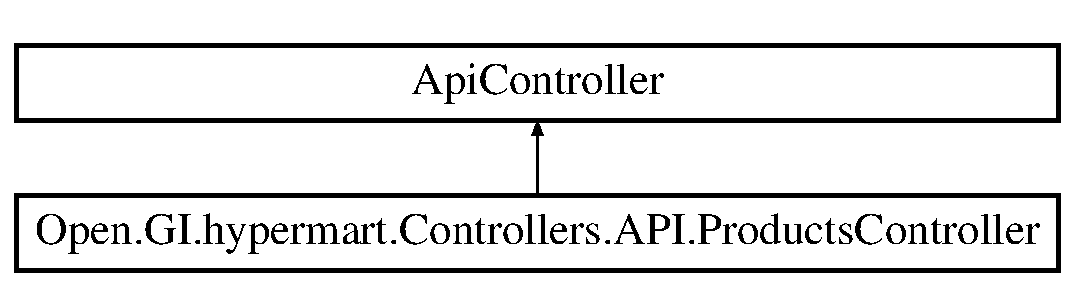
\includegraphics[height=2.000000cm]{class_open_1_1_g_i_1_1hypermart_1_1_controllers_1_1_a_p_i_1_1_products_controller}
\end{center}
\end{figure}
\subsection*{Public Member Functions}
\begin{DoxyCompactItemize}
\item 
\hyperlink{class_open_1_1_g_i_1_1hypermart_1_1_controllers_1_1_a_p_i_1_1_products_controller_ad7451660ccc9180ae0d2bca8e347d426}{Products\+Controller} ()
\begin{DoxyCompactList}\small\item\em Initializes a new instance of the \hyperlink{class_open_1_1_g_i_1_1hypermart_1_1_controllers_1_1_a_p_i_1_1_products_controller}{Products\+Controller} class. \end{DoxyCompactList}\item 
I\+Enumerable$<$ \hyperlink{class_open_1_1_g_i_1_1hypermart_1_1_data_transformation_objects_1_1_product_d_t_o}{Product\+D\+TO} $>$ \hyperlink{class_open_1_1_g_i_1_1hypermart_1_1_controllers_1_1_a_p_i_1_1_products_controller_a717b795b9b5fdecb23a0fcc81b33f34f}{Get\+Products} ()
\begin{DoxyCompactList}\small\item\em Gets the products. \end{DoxyCompactList}\item 
I\+Http\+Action\+Result \hyperlink{class_open_1_1_g_i_1_1hypermart_1_1_controllers_1_1_a_p_i_1_1_products_controller_a68f971a94461093b48568e4f6f38393c}{Get\+Product} (int id)
\begin{DoxyCompactList}\small\item\em Gets the product. \end{DoxyCompactList}\item 
I\+Http\+Action\+Result \hyperlink{class_open_1_1_g_i_1_1hypermart_1_1_controllers_1_1_a_p_i_1_1_products_controller_a13a51589f39ed8e1f7e6b0de1a969ac5}{Put\+Product} (int id, \hyperlink{class_open_1_1_g_i_1_1hypermart_1_1_models_1_1_product}{Product} product)
\begin{DoxyCompactList}\small\item\em Puts the product. \end{DoxyCompactList}\item 
I\+Http\+Action\+Result \hyperlink{class_open_1_1_g_i_1_1hypermart_1_1_controllers_1_1_a_p_i_1_1_products_controller_a0fad687e249ba71420482808c61760e4}{Post\+Product} (\hyperlink{class_open_1_1_g_i_1_1hypermart_1_1_models_1_1_product}{Product} product)
\begin{DoxyCompactList}\small\item\em Posts the product. \end{DoxyCompactList}\item 
I\+Http\+Action\+Result \hyperlink{class_open_1_1_g_i_1_1hypermart_1_1_controllers_1_1_a_p_i_1_1_products_controller_a0c7c45df129f67ada9c5cac65ddd01a3}{Delete\+Product} (int id)
\begin{DoxyCompactList}\small\item\em Deletes the product. \end{DoxyCompactList}\item 
I\+Queryable$<$ \hyperlink{class_open_1_1_g_i_1_1hypermart_1_1_models_1_1_product}{Product} $>$ \hyperlink{class_open_1_1_g_i_1_1hypermart_1_1_controllers_1_1_a_p_i_1_1_products_controller_a5fe504dff28b3f3bdb69623ddd095d93}{Get\+Products} (string Search\+Term)
\begin{DoxyCompactList}\small\item\em Searches for a product. \end{DoxyCompactList}\end{DoxyCompactItemize}
\subsection*{Protected Member Functions}
\begin{DoxyCompactItemize}
\item 
override void \hyperlink{class_open_1_1_g_i_1_1hypermart_1_1_controllers_1_1_a_p_i_1_1_products_controller_a4e48b5e7914c88c15e1187ef6bfb1e09}{Dispose} (bool disposing)
\begin{DoxyCompactList}\small\item\em Releases the unmanaged resources that are used by the object and, optionally, releases the managed resources. \end{DoxyCompactList}\end{DoxyCompactItemize}


\subsection{Detailed Description}
R\+E\+ST \hyperlink{namespace_open_1_1_g_i_1_1hypermart_1_1_controllers_1_1_a_p_i}{A\+PI} layer for interacting with Products. 

\begin{DoxySeeAlso}{See also}
System.\+Web.\+Http.\+Api\+Controller


\end{DoxySeeAlso}


\subsection{Constructor \& Destructor Documentation}
\hypertarget{class_open_1_1_g_i_1_1hypermart_1_1_controllers_1_1_a_p_i_1_1_products_controller_ad7451660ccc9180ae0d2bca8e347d426}{}\label{class_open_1_1_g_i_1_1hypermart_1_1_controllers_1_1_a_p_i_1_1_products_controller_ad7451660ccc9180ae0d2bca8e347d426} 
\index{Open\+::\+G\+I\+::hypermart\+::\+Controllers\+::\+A\+P\+I\+::\+Products\+Controller@{Open\+::\+G\+I\+::hypermart\+::\+Controllers\+::\+A\+P\+I\+::\+Products\+Controller}!Products\+Controller@{Products\+Controller}}
\index{Products\+Controller@{Products\+Controller}!Open\+::\+G\+I\+::hypermart\+::\+Controllers\+::\+A\+P\+I\+::\+Products\+Controller@{Open\+::\+G\+I\+::hypermart\+::\+Controllers\+::\+A\+P\+I\+::\+Products\+Controller}}
\subsubsection{\texorpdfstring{Products\+Controller()}{ProductsController()}}
{\footnotesize\ttfamily Open.\+G\+I.\+hypermart.\+Controllers.\+A\+P\+I.\+Products\+Controller.\+Products\+Controller (\begin{DoxyParamCaption}{ }\end{DoxyParamCaption})}



Initializes a new instance of the \hyperlink{class_open_1_1_g_i_1_1hypermart_1_1_controllers_1_1_a_p_i_1_1_products_controller}{Products\+Controller} class. 



\subsection{Member Function Documentation}
\hypertarget{class_open_1_1_g_i_1_1hypermart_1_1_controllers_1_1_a_p_i_1_1_products_controller_a0c7c45df129f67ada9c5cac65ddd01a3}{}\label{class_open_1_1_g_i_1_1hypermart_1_1_controllers_1_1_a_p_i_1_1_products_controller_a0c7c45df129f67ada9c5cac65ddd01a3} 
\index{Open\+::\+G\+I\+::hypermart\+::\+Controllers\+::\+A\+P\+I\+::\+Products\+Controller@{Open\+::\+G\+I\+::hypermart\+::\+Controllers\+::\+A\+P\+I\+::\+Products\+Controller}!Delete\+Product@{Delete\+Product}}
\index{Delete\+Product@{Delete\+Product}!Open\+::\+G\+I\+::hypermart\+::\+Controllers\+::\+A\+P\+I\+::\+Products\+Controller@{Open\+::\+G\+I\+::hypermart\+::\+Controllers\+::\+A\+P\+I\+::\+Products\+Controller}}
\subsubsection{\texorpdfstring{Delete\+Product()}{DeleteProduct()}}
{\footnotesize\ttfamily I\+Http\+Action\+Result Open.\+G\+I.\+hypermart.\+Controllers.\+A\+P\+I.\+Products\+Controller.\+Delete\+Product (\begin{DoxyParamCaption}\item[{int}]{id }\end{DoxyParamCaption})}



Deletes the product. 


\begin{DoxyParams}{Parameters}
{\em id} & The identifier.\\
\hline
\end{DoxyParams}
\begin{DoxyReturn}{Returns}

\end{DoxyReturn}
\hypertarget{class_open_1_1_g_i_1_1hypermart_1_1_controllers_1_1_a_p_i_1_1_products_controller_a4e48b5e7914c88c15e1187ef6bfb1e09}{}\label{class_open_1_1_g_i_1_1hypermart_1_1_controllers_1_1_a_p_i_1_1_products_controller_a4e48b5e7914c88c15e1187ef6bfb1e09} 
\index{Open\+::\+G\+I\+::hypermart\+::\+Controllers\+::\+A\+P\+I\+::\+Products\+Controller@{Open\+::\+G\+I\+::hypermart\+::\+Controllers\+::\+A\+P\+I\+::\+Products\+Controller}!Dispose@{Dispose}}
\index{Dispose@{Dispose}!Open\+::\+G\+I\+::hypermart\+::\+Controllers\+::\+A\+P\+I\+::\+Products\+Controller@{Open\+::\+G\+I\+::hypermart\+::\+Controllers\+::\+A\+P\+I\+::\+Products\+Controller}}
\subsubsection{\texorpdfstring{Dispose()}{Dispose()}}
{\footnotesize\ttfamily override void Open.\+G\+I.\+hypermart.\+Controllers.\+A\+P\+I.\+Products\+Controller.\+Dispose (\begin{DoxyParamCaption}\item[{bool}]{disposing }\end{DoxyParamCaption})\hspace{0.3cm}{\ttfamily [protected]}}



Releases the unmanaged resources that are used by the object and, optionally, releases the managed resources. 


\begin{DoxyParams}{Parameters}
{\em disposing} & true to release both managed and unmanaged resources; false to release only unmanaged resources.\\
\hline
\end{DoxyParams}
\hypertarget{class_open_1_1_g_i_1_1hypermart_1_1_controllers_1_1_a_p_i_1_1_products_controller_a68f971a94461093b48568e4f6f38393c}{}\label{class_open_1_1_g_i_1_1hypermart_1_1_controllers_1_1_a_p_i_1_1_products_controller_a68f971a94461093b48568e4f6f38393c} 
\index{Open\+::\+G\+I\+::hypermart\+::\+Controllers\+::\+A\+P\+I\+::\+Products\+Controller@{Open\+::\+G\+I\+::hypermart\+::\+Controllers\+::\+A\+P\+I\+::\+Products\+Controller}!Get\+Product@{Get\+Product}}
\index{Get\+Product@{Get\+Product}!Open\+::\+G\+I\+::hypermart\+::\+Controllers\+::\+A\+P\+I\+::\+Products\+Controller@{Open\+::\+G\+I\+::hypermart\+::\+Controllers\+::\+A\+P\+I\+::\+Products\+Controller}}
\subsubsection{\texorpdfstring{Get\+Product()}{GetProduct()}}
{\footnotesize\ttfamily I\+Http\+Action\+Result Open.\+G\+I.\+hypermart.\+Controllers.\+A\+P\+I.\+Products\+Controller.\+Get\+Product (\begin{DoxyParamCaption}\item[{int}]{id }\end{DoxyParamCaption})}



Gets the product. 


\begin{DoxyParams}{Parameters}
{\em id} & The identifier.\\
\hline
\end{DoxyParams}
\begin{DoxyReturn}{Returns}

\end{DoxyReturn}
\hypertarget{class_open_1_1_g_i_1_1hypermart_1_1_controllers_1_1_a_p_i_1_1_products_controller_a717b795b9b5fdecb23a0fcc81b33f34f}{}\label{class_open_1_1_g_i_1_1hypermart_1_1_controllers_1_1_a_p_i_1_1_products_controller_a717b795b9b5fdecb23a0fcc81b33f34f} 
\index{Open\+::\+G\+I\+::hypermart\+::\+Controllers\+::\+A\+P\+I\+::\+Products\+Controller@{Open\+::\+G\+I\+::hypermart\+::\+Controllers\+::\+A\+P\+I\+::\+Products\+Controller}!Get\+Products@{Get\+Products}}
\index{Get\+Products@{Get\+Products}!Open\+::\+G\+I\+::hypermart\+::\+Controllers\+::\+A\+P\+I\+::\+Products\+Controller@{Open\+::\+G\+I\+::hypermart\+::\+Controllers\+::\+A\+P\+I\+::\+Products\+Controller}}
\subsubsection{\texorpdfstring{Get\+Products()}{GetProducts()}\hspace{0.1cm}{\footnotesize\ttfamily [1/2]}}
{\footnotesize\ttfamily I\+Enumerable$<$\hyperlink{class_open_1_1_g_i_1_1hypermart_1_1_data_transformation_objects_1_1_product_d_t_o}{Product\+D\+TO}$>$ Open.\+G\+I.\+hypermart.\+Controllers.\+A\+P\+I.\+Products\+Controller.\+Get\+Products (\begin{DoxyParamCaption}{ }\end{DoxyParamCaption})}



Gets the products. 

\begin{DoxyReturn}{Returns}

\end{DoxyReturn}
\hypertarget{class_open_1_1_g_i_1_1hypermart_1_1_controllers_1_1_a_p_i_1_1_products_controller_a5fe504dff28b3f3bdb69623ddd095d93}{}\label{class_open_1_1_g_i_1_1hypermart_1_1_controllers_1_1_a_p_i_1_1_products_controller_a5fe504dff28b3f3bdb69623ddd095d93} 
\index{Open\+::\+G\+I\+::hypermart\+::\+Controllers\+::\+A\+P\+I\+::\+Products\+Controller@{Open\+::\+G\+I\+::hypermart\+::\+Controllers\+::\+A\+P\+I\+::\+Products\+Controller}!Get\+Products@{Get\+Products}}
\index{Get\+Products@{Get\+Products}!Open\+::\+G\+I\+::hypermart\+::\+Controllers\+::\+A\+P\+I\+::\+Products\+Controller@{Open\+::\+G\+I\+::hypermart\+::\+Controllers\+::\+A\+P\+I\+::\+Products\+Controller}}
\subsubsection{\texorpdfstring{Get\+Products()}{GetProducts()}\hspace{0.1cm}{\footnotesize\ttfamily [2/2]}}
{\footnotesize\ttfamily I\+Queryable$<$\hyperlink{class_open_1_1_g_i_1_1hypermart_1_1_models_1_1_product}{Product}$>$ Open.\+G\+I.\+hypermart.\+Controllers.\+A\+P\+I.\+Products\+Controller.\+Get\+Products (\begin{DoxyParamCaption}\item[{string}]{Search\+Term }\end{DoxyParamCaption})}



Searches for a product. 

\begin{DoxyReturn}{Returns}

\end{DoxyReturn}
\hypertarget{class_open_1_1_g_i_1_1hypermart_1_1_controllers_1_1_a_p_i_1_1_products_controller_a0fad687e249ba71420482808c61760e4}{}\label{class_open_1_1_g_i_1_1hypermart_1_1_controllers_1_1_a_p_i_1_1_products_controller_a0fad687e249ba71420482808c61760e4} 
\index{Open\+::\+G\+I\+::hypermart\+::\+Controllers\+::\+A\+P\+I\+::\+Products\+Controller@{Open\+::\+G\+I\+::hypermart\+::\+Controllers\+::\+A\+P\+I\+::\+Products\+Controller}!Post\+Product@{Post\+Product}}
\index{Post\+Product@{Post\+Product}!Open\+::\+G\+I\+::hypermart\+::\+Controllers\+::\+A\+P\+I\+::\+Products\+Controller@{Open\+::\+G\+I\+::hypermart\+::\+Controllers\+::\+A\+P\+I\+::\+Products\+Controller}}
\subsubsection{\texorpdfstring{Post\+Product()}{PostProduct()}}
{\footnotesize\ttfamily I\+Http\+Action\+Result Open.\+G\+I.\+hypermart.\+Controllers.\+A\+P\+I.\+Products\+Controller.\+Post\+Product (\begin{DoxyParamCaption}\item[{\hyperlink{class_open_1_1_g_i_1_1hypermart_1_1_models_1_1_product}{Product}}]{product }\end{DoxyParamCaption})}



Posts the product. 


\begin{DoxyParams}{Parameters}
{\em product} & The product.\\
\hline
\end{DoxyParams}
\begin{DoxyReturn}{Returns}

\end{DoxyReturn}
\hypertarget{class_open_1_1_g_i_1_1hypermart_1_1_controllers_1_1_a_p_i_1_1_products_controller_a13a51589f39ed8e1f7e6b0de1a969ac5}{}\label{class_open_1_1_g_i_1_1hypermart_1_1_controllers_1_1_a_p_i_1_1_products_controller_a13a51589f39ed8e1f7e6b0de1a969ac5} 
\index{Open\+::\+G\+I\+::hypermart\+::\+Controllers\+::\+A\+P\+I\+::\+Products\+Controller@{Open\+::\+G\+I\+::hypermart\+::\+Controllers\+::\+A\+P\+I\+::\+Products\+Controller}!Put\+Product@{Put\+Product}}
\index{Put\+Product@{Put\+Product}!Open\+::\+G\+I\+::hypermart\+::\+Controllers\+::\+A\+P\+I\+::\+Products\+Controller@{Open\+::\+G\+I\+::hypermart\+::\+Controllers\+::\+A\+P\+I\+::\+Products\+Controller}}
\subsubsection{\texorpdfstring{Put\+Product()}{PutProduct()}}
{\footnotesize\ttfamily I\+Http\+Action\+Result Open.\+G\+I.\+hypermart.\+Controllers.\+A\+P\+I.\+Products\+Controller.\+Put\+Product (\begin{DoxyParamCaption}\item[{int}]{id,  }\item[{\hyperlink{class_open_1_1_g_i_1_1hypermart_1_1_models_1_1_product}{Product}}]{product }\end{DoxyParamCaption})}



Puts the product. 


\begin{DoxyParams}{Parameters}
{\em id} & The identifier.\\
\hline
{\em product} & The product.\\
\hline
\end{DoxyParams}
\begin{DoxyReturn}{Returns}

\end{DoxyReturn}


The documentation for this class was generated from the following file\+:\begin{DoxyCompactItemize}
\item 
C\+:/\+Projects/\+App-\/\+Utility-\/\+Store/\+Open.\+G\+I.\+hypermart/\+Controllers/\+A\+P\+I/\hyperlink{_a_p_i_2_products_controller_8cs}{Products\+Controller.\+cs}\end{DoxyCompactItemize}

\hypertarget{class_open_1_1_g_i_1_1hypermart_1_1_models_1_1_rating}{}\section{Open.\+G\+I.\+hypermart.\+Models.\+Rating Class Reference}
\label{class_open_1_1_g_i_1_1hypermart_1_1_models_1_1_rating}\index{Open.\+G\+I.\+hypermart.\+Models.\+Rating@{Open.\+G\+I.\+hypermart.\+Models.\+Rating}}


Model for storing rating information  


\subsection*{Properties}
\begin{DoxyCompactItemize}
\item 
string \hyperlink{class_open_1_1_g_i_1_1hypermart_1_1_models_1_1_rating_a1e8a569cc68356a222db0eee305273f2}{user\+ID}\hspace{0.3cm}{\ttfamily  \mbox{[}get, set\mbox{]}}
\begin{DoxyCompactList}\small\item\em Gets or sets the user identifier. \end{DoxyCompactList}\item 
string \hyperlink{class_open_1_1_g_i_1_1hypermart_1_1_models_1_1_rating_a89b742b6bfd7d9aa0929b73c951fb37e}{Rating\+Category}\hspace{0.3cm}{\ttfamily  \mbox{[}get, set\mbox{]}}
\begin{DoxyCompactList}\small\item\em Gets or sets the rating category. \end{DoxyCompactList}\item 
int \hyperlink{class_open_1_1_g_i_1_1hypermart_1_1_models_1_1_rating_a84ebcfe9c03b3ee3859323be1a9b02da}{Product\+ID}\hspace{0.3cm}{\ttfamily  \mbox{[}get, set\mbox{]}}
\begin{DoxyCompactList}\small\item\em Gets or sets the product identifier. \end{DoxyCompactList}\item 
\hyperlink{class_open_1_1_g_i_1_1hypermart_1_1_models_1_1_product}{Product} \hyperlink{class_open_1_1_g_i_1_1hypermart_1_1_models_1_1_rating_acf0485f546d4d61e33703627040247e8}{Rated\+Product}\hspace{0.3cm}{\ttfamily  \mbox{[}get, set\mbox{]}}
\begin{DoxyCompactList}\small\item\em Gets or sets the rated product. \end{DoxyCompactList}\item 
double \hyperlink{class_open_1_1_g_i_1_1hypermart_1_1_models_1_1_rating_a1090f6d360b3768ba5ad879befb798e0}{rating}\hspace{0.3cm}{\ttfamily  \mbox{[}get, set\mbox{]}}
\begin{DoxyCompactList}\small\item\em Gets or sets the rating. \end{DoxyCompactList}\item 
string \hyperlink{class_open_1_1_g_i_1_1hypermart_1_1_models_1_1_rating_a1b1467d2d1898f6109cc19ec24ee7fd4}{Comments}\hspace{0.3cm}{\ttfamily  \mbox{[}get, set\mbox{]}}
\begin{DoxyCompactList}\small\item\em Gets or sets the comments. \end{DoxyCompactList}\end{DoxyCompactItemize}


\subsection{Detailed Description}
Model for storing rating information 



\subsection{Property Documentation}
\hypertarget{class_open_1_1_g_i_1_1hypermart_1_1_models_1_1_rating_a1b1467d2d1898f6109cc19ec24ee7fd4}{}\label{class_open_1_1_g_i_1_1hypermart_1_1_models_1_1_rating_a1b1467d2d1898f6109cc19ec24ee7fd4} 
\index{Open\+::\+G\+I\+::hypermart\+::\+Models\+::\+Rating@{Open\+::\+G\+I\+::hypermart\+::\+Models\+::\+Rating}!Comments@{Comments}}
\index{Comments@{Comments}!Open\+::\+G\+I\+::hypermart\+::\+Models\+::\+Rating@{Open\+::\+G\+I\+::hypermart\+::\+Models\+::\+Rating}}
\subsubsection{\texorpdfstring{Comments}{Comments}}
{\footnotesize\ttfamily string Open.\+G\+I.\+hypermart.\+Models.\+Rating.\+Comments\hspace{0.3cm}{\ttfamily [get]}, {\ttfamily [set]}}



Gets or sets the comments. 

The comments. \hypertarget{class_open_1_1_g_i_1_1hypermart_1_1_models_1_1_rating_a84ebcfe9c03b3ee3859323be1a9b02da}{}\label{class_open_1_1_g_i_1_1hypermart_1_1_models_1_1_rating_a84ebcfe9c03b3ee3859323be1a9b02da} 
\index{Open\+::\+G\+I\+::hypermart\+::\+Models\+::\+Rating@{Open\+::\+G\+I\+::hypermart\+::\+Models\+::\+Rating}!Product\+ID@{Product\+ID}}
\index{Product\+ID@{Product\+ID}!Open\+::\+G\+I\+::hypermart\+::\+Models\+::\+Rating@{Open\+::\+G\+I\+::hypermart\+::\+Models\+::\+Rating}}
\subsubsection{\texorpdfstring{Product\+ID}{ProductID}}
{\footnotesize\ttfamily int Open.\+G\+I.\+hypermart.\+Models.\+Rating.\+Product\+ID\hspace{0.3cm}{\ttfamily [get]}, {\ttfamily [set]}}



Gets or sets the product identifier. 

The product identifier. \hypertarget{class_open_1_1_g_i_1_1hypermart_1_1_models_1_1_rating_acf0485f546d4d61e33703627040247e8}{}\label{class_open_1_1_g_i_1_1hypermart_1_1_models_1_1_rating_acf0485f546d4d61e33703627040247e8} 
\index{Open\+::\+G\+I\+::hypermart\+::\+Models\+::\+Rating@{Open\+::\+G\+I\+::hypermart\+::\+Models\+::\+Rating}!Rated\+Product@{Rated\+Product}}
\index{Rated\+Product@{Rated\+Product}!Open\+::\+G\+I\+::hypermart\+::\+Models\+::\+Rating@{Open\+::\+G\+I\+::hypermart\+::\+Models\+::\+Rating}}
\subsubsection{\texorpdfstring{Rated\+Product}{RatedProduct}}
{\footnotesize\ttfamily \hyperlink{class_open_1_1_g_i_1_1hypermart_1_1_models_1_1_product}{Product} Open.\+G\+I.\+hypermart.\+Models.\+Rating.\+Rated\+Product\hspace{0.3cm}{\ttfamily [get]}, {\ttfamily [set]}}



Gets or sets the rated product. 

The rated product. \hypertarget{class_open_1_1_g_i_1_1hypermart_1_1_models_1_1_rating_a1090f6d360b3768ba5ad879befb798e0}{}\label{class_open_1_1_g_i_1_1hypermart_1_1_models_1_1_rating_a1090f6d360b3768ba5ad879befb798e0} 
\index{Open\+::\+G\+I\+::hypermart\+::\+Models\+::\+Rating@{Open\+::\+G\+I\+::hypermart\+::\+Models\+::\+Rating}!rating@{rating}}
\index{rating@{rating}!Open\+::\+G\+I\+::hypermart\+::\+Models\+::\+Rating@{Open\+::\+G\+I\+::hypermart\+::\+Models\+::\+Rating}}
\subsubsection{\texorpdfstring{rating}{rating}}
{\footnotesize\ttfamily double Open.\+G\+I.\+hypermart.\+Models.\+Rating.\+rating\hspace{0.3cm}{\ttfamily [get]}, {\ttfamily [set]}}



Gets or sets the rating. 

The rating. \hypertarget{class_open_1_1_g_i_1_1hypermart_1_1_models_1_1_rating_a89b742b6bfd7d9aa0929b73c951fb37e}{}\label{class_open_1_1_g_i_1_1hypermart_1_1_models_1_1_rating_a89b742b6bfd7d9aa0929b73c951fb37e} 
\index{Open\+::\+G\+I\+::hypermart\+::\+Models\+::\+Rating@{Open\+::\+G\+I\+::hypermart\+::\+Models\+::\+Rating}!Rating\+Category@{Rating\+Category}}
\index{Rating\+Category@{Rating\+Category}!Open\+::\+G\+I\+::hypermart\+::\+Models\+::\+Rating@{Open\+::\+G\+I\+::hypermart\+::\+Models\+::\+Rating}}
\subsubsection{\texorpdfstring{Rating\+Category}{RatingCategory}}
{\footnotesize\ttfamily string Open.\+G\+I.\+hypermart.\+Models.\+Rating.\+Rating\+Category\hspace{0.3cm}{\ttfamily [get]}, {\ttfamily [set]}}



Gets or sets the rating category. 

The rating category. \hypertarget{class_open_1_1_g_i_1_1hypermart_1_1_models_1_1_rating_a1e8a569cc68356a222db0eee305273f2}{}\label{class_open_1_1_g_i_1_1hypermart_1_1_models_1_1_rating_a1e8a569cc68356a222db0eee305273f2} 
\index{Open\+::\+G\+I\+::hypermart\+::\+Models\+::\+Rating@{Open\+::\+G\+I\+::hypermart\+::\+Models\+::\+Rating}!user\+ID@{user\+ID}}
\index{user\+ID@{user\+ID}!Open\+::\+G\+I\+::hypermart\+::\+Models\+::\+Rating@{Open\+::\+G\+I\+::hypermart\+::\+Models\+::\+Rating}}
\subsubsection{\texorpdfstring{user\+ID}{userID}}
{\footnotesize\ttfamily string Open.\+G\+I.\+hypermart.\+Models.\+Rating.\+user\+ID\hspace{0.3cm}{\ttfamily [get]}, {\ttfamily [set]}}



Gets or sets the user identifier. 

The user identifier. 

The documentation for this class was generated from the following file\+:\begin{DoxyCompactItemize}
\item 
C\+:/\+Projects/\+App-\/\+Utility-\/\+Store/\+Open.\+G\+I.\+hypermart/\+Models/\hyperlink{_rating_8cs}{Rating.\+cs}\end{DoxyCompactItemize}

\hypertarget{class_open_1_1_g_i_1_1hypermart_1_1_models_1_1_rating_details}{}\section{Open.\+G\+I.\+hypermart.\+Models.\+Rating\+Details Class Reference}
\label{class_open_1_1_g_i_1_1hypermart_1_1_models_1_1_rating_details}\index{Open.\+G\+I.\+hypermart.\+Models.\+Rating\+Details@{Open.\+G\+I.\+hypermart.\+Models.\+Rating\+Details}}


Model for storing rating information  


\subsection*{Properties}
\begin{DoxyCompactItemize}
\item 
string \hyperlink{class_open_1_1_g_i_1_1hypermart_1_1_models_1_1_rating_details_aafdd0169f033f4d9f2ccc055f938c524}{user\+ID}\hspace{0.3cm}{\ttfamily  \mbox{[}get, set\mbox{]}}
\begin{DoxyCompactList}\small\item\em Gets or sets the user identifier. \end{DoxyCompactList}\item 
string \hyperlink{class_open_1_1_g_i_1_1hypermart_1_1_models_1_1_rating_details_a3c293c7912e7c60b75128586706db64a}{Rating\+Category}\hspace{0.3cm}{\ttfamily  \mbox{[}get, set\mbox{]}}
\begin{DoxyCompactList}\small\item\em Gets or sets the rating category. \end{DoxyCompactList}\item 
int \hyperlink{class_open_1_1_g_i_1_1hypermart_1_1_models_1_1_rating_details_a52049471fb02928fdd8f3b3d9c127a43}{Product\+ID}\hspace{0.3cm}{\ttfamily  \mbox{[}get, set\mbox{]}}
\begin{DoxyCompactList}\small\item\em Gets or sets the product identifier. \end{DoxyCompactList}\item 
\hyperlink{class_open_1_1_g_i_1_1hypermart_1_1_models_1_1_product}{Product} \hyperlink{class_open_1_1_g_i_1_1hypermart_1_1_models_1_1_rating_details_a56011ceff140008b151d983b78371002}{Rated\+Product}\hspace{0.3cm}{\ttfamily  \mbox{[}get, set\mbox{]}}
\begin{DoxyCompactList}\small\item\em Gets or sets the rated product. \end{DoxyCompactList}\item 
int \hyperlink{class_open_1_1_g_i_1_1hypermart_1_1_models_1_1_rating_details_a4ebc3ade419dafcd0571436f6b6363b8}{rating}\hspace{0.3cm}{\ttfamily  \mbox{[}get, set\mbox{]}}
\begin{DoxyCompactList}\small\item\em Gets or sets the rating. \end{DoxyCompactList}\end{DoxyCompactItemize}


\subsection{Detailed Description}
Model for storing rating information 



\subsection{Property Documentation}
\hypertarget{class_open_1_1_g_i_1_1hypermart_1_1_models_1_1_rating_details_a52049471fb02928fdd8f3b3d9c127a43}{}\label{class_open_1_1_g_i_1_1hypermart_1_1_models_1_1_rating_details_a52049471fb02928fdd8f3b3d9c127a43} 
\index{Open\+::\+G\+I\+::hypermart\+::\+Models\+::\+Rating\+Details@{Open\+::\+G\+I\+::hypermart\+::\+Models\+::\+Rating\+Details}!Product\+ID@{Product\+ID}}
\index{Product\+ID@{Product\+ID}!Open\+::\+G\+I\+::hypermart\+::\+Models\+::\+Rating\+Details@{Open\+::\+G\+I\+::hypermart\+::\+Models\+::\+Rating\+Details}}
\subsubsection{\texorpdfstring{Product\+ID}{ProductID}}
{\footnotesize\ttfamily int Open.\+G\+I.\+hypermart.\+Models.\+Rating\+Details.\+Product\+ID\hspace{0.3cm}{\ttfamily [get]}, {\ttfamily [set]}}



Gets or sets the product identifier. 

The product identifier. \hypertarget{class_open_1_1_g_i_1_1hypermart_1_1_models_1_1_rating_details_a56011ceff140008b151d983b78371002}{}\label{class_open_1_1_g_i_1_1hypermart_1_1_models_1_1_rating_details_a56011ceff140008b151d983b78371002} 
\index{Open\+::\+G\+I\+::hypermart\+::\+Models\+::\+Rating\+Details@{Open\+::\+G\+I\+::hypermart\+::\+Models\+::\+Rating\+Details}!Rated\+Product@{Rated\+Product}}
\index{Rated\+Product@{Rated\+Product}!Open\+::\+G\+I\+::hypermart\+::\+Models\+::\+Rating\+Details@{Open\+::\+G\+I\+::hypermart\+::\+Models\+::\+Rating\+Details}}
\subsubsection{\texorpdfstring{Rated\+Product}{RatedProduct}}
{\footnotesize\ttfamily \hyperlink{class_open_1_1_g_i_1_1hypermart_1_1_models_1_1_product}{Product} Open.\+G\+I.\+hypermart.\+Models.\+Rating\+Details.\+Rated\+Product\hspace{0.3cm}{\ttfamily [get]}, {\ttfamily [set]}}



Gets or sets the rated product. 

The rated product. \hypertarget{class_open_1_1_g_i_1_1hypermart_1_1_models_1_1_rating_details_a4ebc3ade419dafcd0571436f6b6363b8}{}\label{class_open_1_1_g_i_1_1hypermart_1_1_models_1_1_rating_details_a4ebc3ade419dafcd0571436f6b6363b8} 
\index{Open\+::\+G\+I\+::hypermart\+::\+Models\+::\+Rating\+Details@{Open\+::\+G\+I\+::hypermart\+::\+Models\+::\+Rating\+Details}!rating@{rating}}
\index{rating@{rating}!Open\+::\+G\+I\+::hypermart\+::\+Models\+::\+Rating\+Details@{Open\+::\+G\+I\+::hypermart\+::\+Models\+::\+Rating\+Details}}
\subsubsection{\texorpdfstring{rating}{rating}}
{\footnotesize\ttfamily int Open.\+G\+I.\+hypermart.\+Models.\+Rating\+Details.\+rating\hspace{0.3cm}{\ttfamily [get]}, {\ttfamily [set]}}



Gets or sets the rating. 

The rating. \hypertarget{class_open_1_1_g_i_1_1hypermart_1_1_models_1_1_rating_details_a3c293c7912e7c60b75128586706db64a}{}\label{class_open_1_1_g_i_1_1hypermart_1_1_models_1_1_rating_details_a3c293c7912e7c60b75128586706db64a} 
\index{Open\+::\+G\+I\+::hypermart\+::\+Models\+::\+Rating\+Details@{Open\+::\+G\+I\+::hypermart\+::\+Models\+::\+Rating\+Details}!Rating\+Category@{Rating\+Category}}
\index{Rating\+Category@{Rating\+Category}!Open\+::\+G\+I\+::hypermart\+::\+Models\+::\+Rating\+Details@{Open\+::\+G\+I\+::hypermart\+::\+Models\+::\+Rating\+Details}}
\subsubsection{\texorpdfstring{Rating\+Category}{RatingCategory}}
{\footnotesize\ttfamily string Open.\+G\+I.\+hypermart.\+Models.\+Rating\+Details.\+Rating\+Category\hspace{0.3cm}{\ttfamily [get]}, {\ttfamily [set]}}



Gets or sets the rating category. 

The rating category. \hypertarget{class_open_1_1_g_i_1_1hypermart_1_1_models_1_1_rating_details_aafdd0169f033f4d9f2ccc055f938c524}{}\label{class_open_1_1_g_i_1_1hypermart_1_1_models_1_1_rating_details_aafdd0169f033f4d9f2ccc055f938c524} 
\index{Open\+::\+G\+I\+::hypermart\+::\+Models\+::\+Rating\+Details@{Open\+::\+G\+I\+::hypermart\+::\+Models\+::\+Rating\+Details}!user\+ID@{user\+ID}}
\index{user\+ID@{user\+ID}!Open\+::\+G\+I\+::hypermart\+::\+Models\+::\+Rating\+Details@{Open\+::\+G\+I\+::hypermart\+::\+Models\+::\+Rating\+Details}}
\subsubsection{\texorpdfstring{user\+ID}{userID}}
{\footnotesize\ttfamily string Open.\+G\+I.\+hypermart.\+Models.\+Rating\+Details.\+user\+ID\hspace{0.3cm}{\ttfamily [get]}, {\ttfamily [set]}}



Gets or sets the user identifier. 

The user identifier. 

The documentation for this class was generated from the following file\+:\begin{DoxyCompactItemize}
\item 
C\+:/\+Projects/\+App-\/\+Utility-\/\+Store/\+Open.\+G\+I.\+hypermart/\+Models/\hyperlink{_rating_details_8cs}{Rating\+Details.\+cs}\end{DoxyCompactItemize}

\hypertarget{class_open_1_1_g_i_1_1hypermart_1_1_controllers_1_1_a_p_i_1_1_rating_details_controller}{}\section{Open.\+G\+I.\+hypermart.\+Controllers.\+A\+P\+I.\+Rating\+Details\+Controller Class Reference}
\label{class_open_1_1_g_i_1_1hypermart_1_1_controllers_1_1_a_p_i_1_1_rating_details_controller}\index{Open.\+G\+I.\+hypermart.\+Controllers.\+A\+P\+I.\+Rating\+Details\+Controller@{Open.\+G\+I.\+hypermart.\+Controllers.\+A\+P\+I.\+Rating\+Details\+Controller}}


R\+E\+ST \hyperlink{namespace_open_1_1_g_i_1_1hypermart_1_1_controllers_1_1_a_p_i}{A\+PI} layer for interacting with ratings.  


Inheritance diagram for Open.\+G\+I.\+hypermart.\+Controllers.\+A\+P\+I.\+Rating\+Details\+Controller\+:\begin{figure}[H]
\begin{center}
\leavevmode
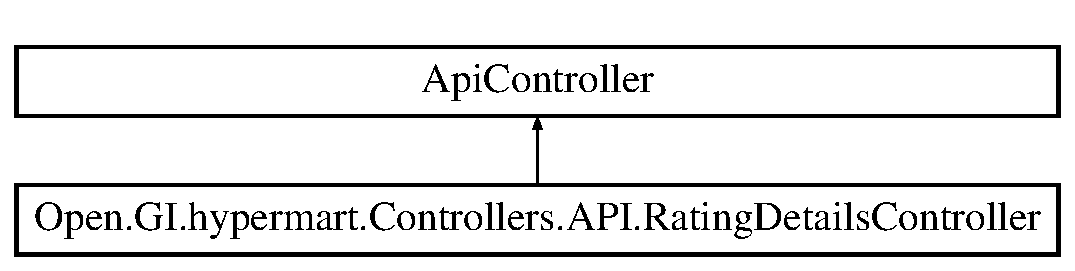
\includegraphics[height=2.000000cm]{class_open_1_1_g_i_1_1hypermart_1_1_controllers_1_1_a_p_i_1_1_rating_details_controller}
\end{center}
\end{figure}
\subsection*{Public Member Functions}
\begin{DoxyCompactItemize}
\item 
\hyperlink{class_open_1_1_g_i_1_1hypermart_1_1_controllers_1_1_a_p_i_1_1_rating_details_controller_ab75ad1214077861b992f7d3cf7159bd1}{Rating\+Details\+Controller} (\hyperlink{class_open_1_1_g_i_1_1hypermart_1_1_d_a_l_1_1_hypermart_context}{Hypermart\+Context} db)
\begin{DoxyCompactList}\small\item\em Initializes a new instance of the \hyperlink{class_open_1_1_g_i_1_1hypermart_1_1_controllers_1_1_a_p_i_1_1_rating_details_controller}{Rating\+Details\+Controller} class. \end{DoxyCompactList}\item 
\hyperlink{class_open_1_1_g_i_1_1hypermart_1_1_controllers_1_1_a_p_i_1_1_rating_details_controller_ae1d1b41f5c7984058a45aec845afcc97}{Rating\+Details\+Controller} ()
\item 
I\+Queryable$<$ \hyperlink{class_open_1_1_g_i_1_1hypermart_1_1_models_1_1_rating_details}{Rating\+Details} $>$ \hyperlink{class_open_1_1_g_i_1_1hypermart_1_1_controllers_1_1_a_p_i_1_1_rating_details_controller_a557eb976767689358889d1728a16c167}{Get\+Rating\+Details} ()
\begin{DoxyCompactList}\small\item\em Gets the rating details. \end{DoxyCompactList}\item 
I\+Http\+Action\+Result \hyperlink{class_open_1_1_g_i_1_1hypermart_1_1_controllers_1_1_a_p_i_1_1_rating_details_controller_a498b197bc682eea0f658ce9b8f44df0e}{Get\+Rating\+Details} (int id)
\begin{DoxyCompactList}\small\item\em Gets the rating details. \end{DoxyCompactList}\item 
I\+Http\+Action\+Result \hyperlink{class_open_1_1_g_i_1_1hypermart_1_1_controllers_1_1_a_p_i_1_1_rating_details_controller_aeaa95bcc98646b2a84205b111b0d2560}{Put\+Rating\+Details} (string id, \hyperlink{class_open_1_1_g_i_1_1hypermart_1_1_models_1_1_rating_details}{Rating\+Details} rating\+Details)
\begin{DoxyCompactList}\small\item\em Puts the rating details. \end{DoxyCompactList}\item 
I\+Http\+Action\+Result \hyperlink{class_open_1_1_g_i_1_1hypermart_1_1_controllers_1_1_a_p_i_1_1_rating_details_controller_a8319f5f58c948de731eac334adcd2e82}{Post\+Rating\+Details} (\hyperlink{class_open_1_1_g_i_1_1hypermart_1_1_models_1_1_rating_details}{Rating\+Details} rating\+Details)
\begin{DoxyCompactList}\small\item\em Posts the rating details. \end{DoxyCompactList}\item 
I\+Http\+Action\+Result \hyperlink{class_open_1_1_g_i_1_1hypermart_1_1_controllers_1_1_a_p_i_1_1_rating_details_controller_aa92516d49a489314191626dc9cdb4a34}{Delete\+Rating\+Details} (string id)
\begin{DoxyCompactList}\small\item\em Deletes the rating details. \end{DoxyCompactList}\end{DoxyCompactItemize}
\subsection*{Protected Member Functions}
\begin{DoxyCompactItemize}
\item 
override void \hyperlink{class_open_1_1_g_i_1_1hypermart_1_1_controllers_1_1_a_p_i_1_1_rating_details_controller_a81ada59de033f14c4758007d4a243644}{Dispose} (bool disposing)
\begin{DoxyCompactList}\small\item\em Releases the unmanaged resources that are used by the object and, optionally, releases the managed resources. \end{DoxyCompactList}\end{DoxyCompactItemize}


\subsection{Detailed Description}
R\+E\+ST \hyperlink{namespace_open_1_1_g_i_1_1hypermart_1_1_controllers_1_1_a_p_i}{A\+PI} layer for interacting with ratings. 

\begin{DoxySeeAlso}{See also}
System.\+Web.\+Http.\+Api\+Controller


\end{DoxySeeAlso}


\subsection{Constructor \& Destructor Documentation}
\hypertarget{class_open_1_1_g_i_1_1hypermart_1_1_controllers_1_1_a_p_i_1_1_rating_details_controller_ab75ad1214077861b992f7d3cf7159bd1}{}\label{class_open_1_1_g_i_1_1hypermart_1_1_controllers_1_1_a_p_i_1_1_rating_details_controller_ab75ad1214077861b992f7d3cf7159bd1} 
\index{Open\+::\+G\+I\+::hypermart\+::\+Controllers\+::\+A\+P\+I\+::\+Rating\+Details\+Controller@{Open\+::\+G\+I\+::hypermart\+::\+Controllers\+::\+A\+P\+I\+::\+Rating\+Details\+Controller}!Rating\+Details\+Controller@{Rating\+Details\+Controller}}
\index{Rating\+Details\+Controller@{Rating\+Details\+Controller}!Open\+::\+G\+I\+::hypermart\+::\+Controllers\+::\+A\+P\+I\+::\+Rating\+Details\+Controller@{Open\+::\+G\+I\+::hypermart\+::\+Controllers\+::\+A\+P\+I\+::\+Rating\+Details\+Controller}}
\subsubsection{\texorpdfstring{Rating\+Details\+Controller()}{RatingDetailsController()}\hspace{0.1cm}{\footnotesize\ttfamily [1/2]}}
{\footnotesize\ttfamily Open.\+G\+I.\+hypermart.\+Controllers.\+A\+P\+I.\+Rating\+Details\+Controller.\+Rating\+Details\+Controller (\begin{DoxyParamCaption}\item[{\hyperlink{class_open_1_1_g_i_1_1hypermart_1_1_d_a_l_1_1_hypermart_context}{Hypermart\+Context}}]{db }\end{DoxyParamCaption})}



Initializes a new instance of the \hyperlink{class_open_1_1_g_i_1_1hypermart_1_1_controllers_1_1_a_p_i_1_1_rating_details_controller}{Rating\+Details\+Controller} class. 


\begin{DoxyParams}{Parameters}
{\em db} & The database.\\
\hline
\end{DoxyParams}
\hypertarget{class_open_1_1_g_i_1_1hypermart_1_1_controllers_1_1_a_p_i_1_1_rating_details_controller_ae1d1b41f5c7984058a45aec845afcc97}{}\label{class_open_1_1_g_i_1_1hypermart_1_1_controllers_1_1_a_p_i_1_1_rating_details_controller_ae1d1b41f5c7984058a45aec845afcc97} 
\index{Open\+::\+G\+I\+::hypermart\+::\+Controllers\+::\+A\+P\+I\+::\+Rating\+Details\+Controller@{Open\+::\+G\+I\+::hypermart\+::\+Controllers\+::\+A\+P\+I\+::\+Rating\+Details\+Controller}!Rating\+Details\+Controller@{Rating\+Details\+Controller}}
\index{Rating\+Details\+Controller@{Rating\+Details\+Controller}!Open\+::\+G\+I\+::hypermart\+::\+Controllers\+::\+A\+P\+I\+::\+Rating\+Details\+Controller@{Open\+::\+G\+I\+::hypermart\+::\+Controllers\+::\+A\+P\+I\+::\+Rating\+Details\+Controller}}
\subsubsection{\texorpdfstring{Rating\+Details\+Controller()}{RatingDetailsController()}\hspace{0.1cm}{\footnotesize\ttfamily [2/2]}}
{\footnotesize\ttfamily Open.\+G\+I.\+hypermart.\+Controllers.\+A\+P\+I.\+Rating\+Details\+Controller.\+Rating\+Details\+Controller (\begin{DoxyParamCaption}{ }\end{DoxyParamCaption})}



\subsection{Member Function Documentation}
\hypertarget{class_open_1_1_g_i_1_1hypermart_1_1_controllers_1_1_a_p_i_1_1_rating_details_controller_aa92516d49a489314191626dc9cdb4a34}{}\label{class_open_1_1_g_i_1_1hypermart_1_1_controllers_1_1_a_p_i_1_1_rating_details_controller_aa92516d49a489314191626dc9cdb4a34} 
\index{Open\+::\+G\+I\+::hypermart\+::\+Controllers\+::\+A\+P\+I\+::\+Rating\+Details\+Controller@{Open\+::\+G\+I\+::hypermart\+::\+Controllers\+::\+A\+P\+I\+::\+Rating\+Details\+Controller}!Delete\+Rating\+Details@{Delete\+Rating\+Details}}
\index{Delete\+Rating\+Details@{Delete\+Rating\+Details}!Open\+::\+G\+I\+::hypermart\+::\+Controllers\+::\+A\+P\+I\+::\+Rating\+Details\+Controller@{Open\+::\+G\+I\+::hypermart\+::\+Controllers\+::\+A\+P\+I\+::\+Rating\+Details\+Controller}}
\subsubsection{\texorpdfstring{Delete\+Rating\+Details()}{DeleteRatingDetails()}}
{\footnotesize\ttfamily I\+Http\+Action\+Result Open.\+G\+I.\+hypermart.\+Controllers.\+A\+P\+I.\+Rating\+Details\+Controller.\+Delete\+Rating\+Details (\begin{DoxyParamCaption}\item[{string}]{id }\end{DoxyParamCaption})}



Deletes the rating details. 


\begin{DoxyParams}{Parameters}
{\em id} & The identifier.\\
\hline
\end{DoxyParams}
\begin{DoxyReturn}{Returns}

\end{DoxyReturn}
\hypertarget{class_open_1_1_g_i_1_1hypermart_1_1_controllers_1_1_a_p_i_1_1_rating_details_controller_a81ada59de033f14c4758007d4a243644}{}\label{class_open_1_1_g_i_1_1hypermart_1_1_controllers_1_1_a_p_i_1_1_rating_details_controller_a81ada59de033f14c4758007d4a243644} 
\index{Open\+::\+G\+I\+::hypermart\+::\+Controllers\+::\+A\+P\+I\+::\+Rating\+Details\+Controller@{Open\+::\+G\+I\+::hypermart\+::\+Controllers\+::\+A\+P\+I\+::\+Rating\+Details\+Controller}!Dispose@{Dispose}}
\index{Dispose@{Dispose}!Open\+::\+G\+I\+::hypermart\+::\+Controllers\+::\+A\+P\+I\+::\+Rating\+Details\+Controller@{Open\+::\+G\+I\+::hypermart\+::\+Controllers\+::\+A\+P\+I\+::\+Rating\+Details\+Controller}}
\subsubsection{\texorpdfstring{Dispose()}{Dispose()}}
{\footnotesize\ttfamily override void Open.\+G\+I.\+hypermart.\+Controllers.\+A\+P\+I.\+Rating\+Details\+Controller.\+Dispose (\begin{DoxyParamCaption}\item[{bool}]{disposing }\end{DoxyParamCaption})\hspace{0.3cm}{\ttfamily [protected]}}



Releases the unmanaged resources that are used by the object and, optionally, releases the managed resources. 


\begin{DoxyParams}{Parameters}
{\em disposing} & true to release both managed and unmanaged resources; false to release only unmanaged resources.\\
\hline
\end{DoxyParams}
\hypertarget{class_open_1_1_g_i_1_1hypermart_1_1_controllers_1_1_a_p_i_1_1_rating_details_controller_a557eb976767689358889d1728a16c167}{}\label{class_open_1_1_g_i_1_1hypermart_1_1_controllers_1_1_a_p_i_1_1_rating_details_controller_a557eb976767689358889d1728a16c167} 
\index{Open\+::\+G\+I\+::hypermart\+::\+Controllers\+::\+A\+P\+I\+::\+Rating\+Details\+Controller@{Open\+::\+G\+I\+::hypermart\+::\+Controllers\+::\+A\+P\+I\+::\+Rating\+Details\+Controller}!Get\+Rating\+Details@{Get\+Rating\+Details}}
\index{Get\+Rating\+Details@{Get\+Rating\+Details}!Open\+::\+G\+I\+::hypermart\+::\+Controllers\+::\+A\+P\+I\+::\+Rating\+Details\+Controller@{Open\+::\+G\+I\+::hypermart\+::\+Controllers\+::\+A\+P\+I\+::\+Rating\+Details\+Controller}}
\subsubsection{\texorpdfstring{Get\+Rating\+Details()}{GetRatingDetails()}\hspace{0.1cm}{\footnotesize\ttfamily [1/2]}}
{\footnotesize\ttfamily I\+Queryable$<$\hyperlink{class_open_1_1_g_i_1_1hypermart_1_1_models_1_1_rating_details}{Rating\+Details}$>$ Open.\+G\+I.\+hypermart.\+Controllers.\+A\+P\+I.\+Rating\+Details\+Controller.\+Get\+Rating\+Details (\begin{DoxyParamCaption}{ }\end{DoxyParamCaption})}



Gets the rating details. 

\begin{DoxyReturn}{Returns}

\end{DoxyReturn}
\hypertarget{class_open_1_1_g_i_1_1hypermart_1_1_controllers_1_1_a_p_i_1_1_rating_details_controller_a498b197bc682eea0f658ce9b8f44df0e}{}\label{class_open_1_1_g_i_1_1hypermart_1_1_controllers_1_1_a_p_i_1_1_rating_details_controller_a498b197bc682eea0f658ce9b8f44df0e} 
\index{Open\+::\+G\+I\+::hypermart\+::\+Controllers\+::\+A\+P\+I\+::\+Rating\+Details\+Controller@{Open\+::\+G\+I\+::hypermart\+::\+Controllers\+::\+A\+P\+I\+::\+Rating\+Details\+Controller}!Get\+Rating\+Details@{Get\+Rating\+Details}}
\index{Get\+Rating\+Details@{Get\+Rating\+Details}!Open\+::\+G\+I\+::hypermart\+::\+Controllers\+::\+A\+P\+I\+::\+Rating\+Details\+Controller@{Open\+::\+G\+I\+::hypermart\+::\+Controllers\+::\+A\+P\+I\+::\+Rating\+Details\+Controller}}
\subsubsection{\texorpdfstring{Get\+Rating\+Details()}{GetRatingDetails()}\hspace{0.1cm}{\footnotesize\ttfamily [2/2]}}
{\footnotesize\ttfamily I\+Http\+Action\+Result Open.\+G\+I.\+hypermart.\+Controllers.\+A\+P\+I.\+Rating\+Details\+Controller.\+Get\+Rating\+Details (\begin{DoxyParamCaption}\item[{int}]{id }\end{DoxyParamCaption})}



Gets the rating details. 


\begin{DoxyParams}{Parameters}
{\em id} & The identifier.\\
\hline
\end{DoxyParams}
\begin{DoxyReturn}{Returns}

\end{DoxyReturn}
\hypertarget{class_open_1_1_g_i_1_1hypermart_1_1_controllers_1_1_a_p_i_1_1_rating_details_controller_a8319f5f58c948de731eac334adcd2e82}{}\label{class_open_1_1_g_i_1_1hypermart_1_1_controllers_1_1_a_p_i_1_1_rating_details_controller_a8319f5f58c948de731eac334adcd2e82} 
\index{Open\+::\+G\+I\+::hypermart\+::\+Controllers\+::\+A\+P\+I\+::\+Rating\+Details\+Controller@{Open\+::\+G\+I\+::hypermart\+::\+Controllers\+::\+A\+P\+I\+::\+Rating\+Details\+Controller}!Post\+Rating\+Details@{Post\+Rating\+Details}}
\index{Post\+Rating\+Details@{Post\+Rating\+Details}!Open\+::\+G\+I\+::hypermart\+::\+Controllers\+::\+A\+P\+I\+::\+Rating\+Details\+Controller@{Open\+::\+G\+I\+::hypermart\+::\+Controllers\+::\+A\+P\+I\+::\+Rating\+Details\+Controller}}
\subsubsection{\texorpdfstring{Post\+Rating\+Details()}{PostRatingDetails()}}
{\footnotesize\ttfamily I\+Http\+Action\+Result Open.\+G\+I.\+hypermart.\+Controllers.\+A\+P\+I.\+Rating\+Details\+Controller.\+Post\+Rating\+Details (\begin{DoxyParamCaption}\item[{\hyperlink{class_open_1_1_g_i_1_1hypermart_1_1_models_1_1_rating_details}{Rating\+Details}}]{rating\+Details }\end{DoxyParamCaption})}



Posts the rating details. 


\begin{DoxyParams}{Parameters}
{\em rating\+Details} & The rating details.\\
\hline
\end{DoxyParams}
\begin{DoxyReturn}{Returns}

\end{DoxyReturn}
\hypertarget{class_open_1_1_g_i_1_1hypermart_1_1_controllers_1_1_a_p_i_1_1_rating_details_controller_aeaa95bcc98646b2a84205b111b0d2560}{}\label{class_open_1_1_g_i_1_1hypermart_1_1_controllers_1_1_a_p_i_1_1_rating_details_controller_aeaa95bcc98646b2a84205b111b0d2560} 
\index{Open\+::\+G\+I\+::hypermart\+::\+Controllers\+::\+A\+P\+I\+::\+Rating\+Details\+Controller@{Open\+::\+G\+I\+::hypermart\+::\+Controllers\+::\+A\+P\+I\+::\+Rating\+Details\+Controller}!Put\+Rating\+Details@{Put\+Rating\+Details}}
\index{Put\+Rating\+Details@{Put\+Rating\+Details}!Open\+::\+G\+I\+::hypermart\+::\+Controllers\+::\+A\+P\+I\+::\+Rating\+Details\+Controller@{Open\+::\+G\+I\+::hypermart\+::\+Controllers\+::\+A\+P\+I\+::\+Rating\+Details\+Controller}}
\subsubsection{\texorpdfstring{Put\+Rating\+Details()}{PutRatingDetails()}}
{\footnotesize\ttfamily I\+Http\+Action\+Result Open.\+G\+I.\+hypermart.\+Controllers.\+A\+P\+I.\+Rating\+Details\+Controller.\+Put\+Rating\+Details (\begin{DoxyParamCaption}\item[{string}]{id,  }\item[{\hyperlink{class_open_1_1_g_i_1_1hypermart_1_1_models_1_1_rating_details}{Rating\+Details}}]{rating\+Details }\end{DoxyParamCaption})}



Puts the rating details. 


\begin{DoxyParams}{Parameters}
{\em id} & The identifier.\\
\hline
{\em rating\+Details} & The rating details.\\
\hline
\end{DoxyParams}
\begin{DoxyReturn}{Returns}

\end{DoxyReturn}


The documentation for this class was generated from the following file\+:\begin{DoxyCompactItemize}
\item 
C\+:/\+Projects/\+App-\/\+Utility-\/\+Store/\+Open.\+G\+I.\+hypermart/\+Controllers/\+A\+P\+I/\hyperlink{_rating_details_controller_8cs}{Rating\+Details\+Controller.\+cs}\end{DoxyCompactItemize}

\section{Open.\+G\+I.\+hypermart.\+Data\+Transformation\+Objects.\+Rating\+D\+TO Class Reference}
\label{class_open_1_1_g_i_1_1hypermart_1_1_data_transformation_objects_1_1_rating_d_t_o}\index{Open.\+G\+I.\+hypermart.\+Data\+Transformation\+Objects.\+Rating\+D\+TO@{Open.\+G\+I.\+hypermart.\+Data\+Transformation\+Objects.\+Rating\+D\+TO}}


Rating detail D\+TO  


\subsection*{Public Member Functions}
\begin{DoxyCompactItemize}
\item 
\textbf{ Rating\+D\+TO} (string \textbf{ Rated\+Area}, int score, int outof)
\begin{DoxyCompactList}\small\item\em Initializes a new instance of the \doxyref{Rating\+D\+TO}{p.}{class_open_1_1_g_i_1_1hypermart_1_1_data_transformation_objects_1_1_rating_d_t_o} class. \end{DoxyCompactList}\end{DoxyCompactItemize}
\subsection*{Properties}
\begin{DoxyCompactItemize}
\item 
string \textbf{ Rated\+Area}\hspace{0.3cm}{\ttfamily  [get, set]}
\begin{DoxyCompactList}\small\item\em Gets or sets the rated area. \end{DoxyCompactList}\item 
int \textbf{ Score}\hspace{0.3cm}{\ttfamily  [get, set]}
\begin{DoxyCompactList}\small\item\em Gets or sets the score. \end{DoxyCompactList}\item 
int \textbf{ Out\+Of}\hspace{0.3cm}{\ttfamily  [get, set]}
\begin{DoxyCompactList}\small\item\em Gets or sets the out of. \end{DoxyCompactList}\end{DoxyCompactItemize}


\subsection{Detailed Description}
Rating detail D\+TO 



Definition at line 12 of file Rating\+D\+T\+O.\+cs.



\subsection{Constructor \& Destructor Documentation}
\mbox{\label{class_open_1_1_g_i_1_1hypermart_1_1_data_transformation_objects_1_1_rating_d_t_o_ab6f971e21c62e4004fdc0b20d1fea033}} 
\index{Open\+::\+G\+I\+::hypermart\+::\+Data\+Transformation\+Objects\+::\+Rating\+D\+TO@{Open\+::\+G\+I\+::hypermart\+::\+Data\+Transformation\+Objects\+::\+Rating\+D\+TO}!Rating\+D\+TO@{Rating\+D\+TO}}
\index{Rating\+D\+TO@{Rating\+D\+TO}!Open\+::\+G\+I\+::hypermart\+::\+Data\+Transformation\+Objects\+::\+Rating\+D\+TO@{Open\+::\+G\+I\+::hypermart\+::\+Data\+Transformation\+Objects\+::\+Rating\+D\+TO}}
\subsubsection{Rating\+D\+T\+O()}
{\footnotesize\ttfamily Open.\+G\+I.\+hypermart.\+Data\+Transformation\+Objects.\+Rating\+D\+T\+O.\+Rating\+D\+TO (\begin{DoxyParamCaption}\item[{string}]{Rated\+Area,  }\item[{int}]{score,  }\item[{int}]{outof }\end{DoxyParamCaption})}



Initializes a new instance of the \doxyref{Rating\+D\+TO}{p.}{class_open_1_1_g_i_1_1hypermart_1_1_data_transformation_objects_1_1_rating_d_t_o} class. 


\begin{DoxyParams}{Parameters}
{\em Rated\+Area} & The rated area.\\
\hline
{\em score} & The score.\\
\hline
{\em outof} & The outof.\\
\hline
\end{DoxyParams}


Definition at line 20 of file Rating\+D\+T\+O.\+cs.



\subsection{Property Documentation}
\mbox{\label{class_open_1_1_g_i_1_1hypermart_1_1_data_transformation_objects_1_1_rating_d_t_o_a3a690d9692b556515be4aa8e2cc0af75}} 
\index{Open\+::\+G\+I\+::hypermart\+::\+Data\+Transformation\+Objects\+::\+Rating\+D\+TO@{Open\+::\+G\+I\+::hypermart\+::\+Data\+Transformation\+Objects\+::\+Rating\+D\+TO}!Out\+Of@{Out\+Of}}
\index{Out\+Of@{Out\+Of}!Open\+::\+G\+I\+::hypermart\+::\+Data\+Transformation\+Objects\+::\+Rating\+D\+TO@{Open\+::\+G\+I\+::hypermart\+::\+Data\+Transformation\+Objects\+::\+Rating\+D\+TO}}
\subsubsection{Out\+Of}
{\footnotesize\ttfamily int Open.\+G\+I.\+hypermart.\+Data\+Transformation\+Objects.\+Rating\+D\+T\+O.\+Out\+Of\hspace{0.3cm}{\ttfamily [get]}, {\ttfamily [set]}}



Gets or sets the out of. 

The out of. 

Definition at line 47 of file Rating\+D\+T\+O.\+cs.

\mbox{\label{class_open_1_1_g_i_1_1hypermart_1_1_data_transformation_objects_1_1_rating_d_t_o_ad3282fe707334d675bc3c99694dff533}} 
\index{Open\+::\+G\+I\+::hypermart\+::\+Data\+Transformation\+Objects\+::\+Rating\+D\+TO@{Open\+::\+G\+I\+::hypermart\+::\+Data\+Transformation\+Objects\+::\+Rating\+D\+TO}!Rated\+Area@{Rated\+Area}}
\index{Rated\+Area@{Rated\+Area}!Open\+::\+G\+I\+::hypermart\+::\+Data\+Transformation\+Objects\+::\+Rating\+D\+TO@{Open\+::\+G\+I\+::hypermart\+::\+Data\+Transformation\+Objects\+::\+Rating\+D\+TO}}
\subsubsection{Rated\+Area}
{\footnotesize\ttfamily string Open.\+G\+I.\+hypermart.\+Data\+Transformation\+Objects.\+Rating\+D\+T\+O.\+Rated\+Area\hspace{0.3cm}{\ttfamily [get]}, {\ttfamily [set]}}



Gets or sets the rated area. 

The rated area. 

Definition at line 33 of file Rating\+D\+T\+O.\+cs.

\mbox{\label{class_open_1_1_g_i_1_1hypermart_1_1_data_transformation_objects_1_1_rating_d_t_o_a8548920a2914900206fe636ca7aa7cbb}} 
\index{Open\+::\+G\+I\+::hypermart\+::\+Data\+Transformation\+Objects\+::\+Rating\+D\+TO@{Open\+::\+G\+I\+::hypermart\+::\+Data\+Transformation\+Objects\+::\+Rating\+D\+TO}!Score@{Score}}
\index{Score@{Score}!Open\+::\+G\+I\+::hypermart\+::\+Data\+Transformation\+Objects\+::\+Rating\+D\+TO@{Open\+::\+G\+I\+::hypermart\+::\+Data\+Transformation\+Objects\+::\+Rating\+D\+TO}}
\subsubsection{Score}
{\footnotesize\ttfamily int Open.\+G\+I.\+hypermart.\+Data\+Transformation\+Objects.\+Rating\+D\+T\+O.\+Score\hspace{0.3cm}{\ttfamily [get]}, {\ttfamily [set]}}



Gets or sets the score. 

The score. 

Definition at line 40 of file Rating\+D\+T\+O.\+cs.



The documentation for this class was generated from the following file\+:\begin{DoxyCompactItemize}
\item 
C\+:/\+Projects/\+App-\/\+Utility-\/\+Store/\+Open.\+G\+I.\+hypermart/\+Docs/\+Data\+Transformation\+Objects/\textbf{ Rating\+D\+T\+O.\+cs}\end{DoxyCompactItemize}

\section{Open.\+G\+I.\+hypermart.\+Data\+Transformation\+Objects.\+Rating\+Information\+D\+TO Class Reference}
\label{class_open_1_1_g_i_1_1hypermart_1_1_data_transformation_objects_1_1_rating_information_d_t_o}\index{Open.\+G\+I.\+hypermart.\+Data\+Transformation\+Objects.\+Rating\+Information\+D\+TO@{Open.\+G\+I.\+hypermart.\+Data\+Transformation\+Objects.\+Rating\+Information\+D\+TO}}


Rating information D\+TO  


\subsection*{Public Member Functions}
\begin{DoxyCompactItemize}
\item 
\textbf{ Rating\+Information\+D\+TO} ()
\begin{DoxyCompactList}\small\item\em Initializes a new instance of the \doxyref{Rating\+Information\+D\+TO}{p.}{class_open_1_1_g_i_1_1hypermart_1_1_data_transformation_objects_1_1_rating_information_d_t_o} class. \end{DoxyCompactList}\end{DoxyCompactItemize}
\subsection*{Properties}
\begin{DoxyCompactItemize}
\item 
int \textbf{ Product\+ID}\hspace{0.3cm}{\ttfamily  [get, set]}
\begin{DoxyCompactList}\small\item\em Gets or sets the product identifier. \end{DoxyCompactList}\item 
int \textbf{ File\+ID}\hspace{0.3cm}{\ttfamily  [get, set]}
\begin{DoxyCompactList}\small\item\em Gets or sets the file identifier. \end{DoxyCompactList}\item 
List$<$ \textbf{ Rating\+D\+TO} $>$ \textbf{ Ratings}\hspace{0.3cm}{\ttfamily  [get, set]}
\begin{DoxyCompactList}\small\item\em Gets or sets the ratings. \end{DoxyCompactList}\item 
string \textbf{ Comment\+Title}\hspace{0.3cm}{\ttfamily  [get, set]}
\begin{DoxyCompactList}\small\item\em Gets or sets the comment title. \end{DoxyCompactList}\item 
string \textbf{ Comment}\hspace{0.3cm}{\ttfamily  [get, set]}
\begin{DoxyCompactList}\small\item\em Gets or sets the comment. \end{DoxyCompactList}\end{DoxyCompactItemize}


\subsection{Detailed Description}
Rating information D\+TO 



Definition at line 12 of file Rating\+Information\+D\+T\+O.\+cs.



\subsection{Constructor \& Destructor Documentation}
\mbox{\label{class_open_1_1_g_i_1_1hypermart_1_1_data_transformation_objects_1_1_rating_information_d_t_o_a51c542e9651681efa2e577a9d02195c6}} 
\index{Open\+::\+G\+I\+::hypermart\+::\+Data\+Transformation\+Objects\+::\+Rating\+Information\+D\+TO@{Open\+::\+G\+I\+::hypermart\+::\+Data\+Transformation\+Objects\+::\+Rating\+Information\+D\+TO}!Rating\+Information\+D\+TO@{Rating\+Information\+D\+TO}}
\index{Rating\+Information\+D\+TO@{Rating\+Information\+D\+TO}!Open\+::\+G\+I\+::hypermart\+::\+Data\+Transformation\+Objects\+::\+Rating\+Information\+D\+TO@{Open\+::\+G\+I\+::hypermart\+::\+Data\+Transformation\+Objects\+::\+Rating\+Information\+D\+TO}}
\subsubsection{Rating\+Information\+D\+T\+O()}
{\footnotesize\ttfamily Open.\+G\+I.\+hypermart.\+Data\+Transformation\+Objects.\+Rating\+Information\+D\+T\+O.\+Rating\+Information\+D\+TO (\begin{DoxyParamCaption}{ }\end{DoxyParamCaption})}



Initializes a new instance of the \doxyref{Rating\+Information\+D\+TO}{p.}{class_open_1_1_g_i_1_1hypermart_1_1_data_transformation_objects_1_1_rating_information_d_t_o} class. 



Definition at line 17 of file Rating\+Information\+D\+T\+O.\+cs.



\subsection{Property Documentation}
\mbox{\label{class_open_1_1_g_i_1_1hypermart_1_1_data_transformation_objects_1_1_rating_information_d_t_o_a75cc38ad71428e87e97db4d9c1deb672}} 
\index{Open\+::\+G\+I\+::hypermart\+::\+Data\+Transformation\+Objects\+::\+Rating\+Information\+D\+TO@{Open\+::\+G\+I\+::hypermart\+::\+Data\+Transformation\+Objects\+::\+Rating\+Information\+D\+TO}!Comment@{Comment}}
\index{Comment@{Comment}!Open\+::\+G\+I\+::hypermart\+::\+Data\+Transformation\+Objects\+::\+Rating\+Information\+D\+TO@{Open\+::\+G\+I\+::hypermart\+::\+Data\+Transformation\+Objects\+::\+Rating\+Information\+D\+TO}}
\subsubsection{Comment}
{\footnotesize\ttfamily string Open.\+G\+I.\+hypermart.\+Data\+Transformation\+Objects.\+Rating\+Information\+D\+T\+O.\+Comment\hspace{0.3cm}{\ttfamily [get]}, {\ttfamily [set]}}



Gets or sets the comment. 

The comment. 

Definition at line 55 of file Rating\+Information\+D\+T\+O.\+cs.

\mbox{\label{class_open_1_1_g_i_1_1hypermart_1_1_data_transformation_objects_1_1_rating_information_d_t_o_aa7dbcf1f467890a811b458b76c68e7f5}} 
\index{Open\+::\+G\+I\+::hypermart\+::\+Data\+Transformation\+Objects\+::\+Rating\+Information\+D\+TO@{Open\+::\+G\+I\+::hypermart\+::\+Data\+Transformation\+Objects\+::\+Rating\+Information\+D\+TO}!Comment\+Title@{Comment\+Title}}
\index{Comment\+Title@{Comment\+Title}!Open\+::\+G\+I\+::hypermart\+::\+Data\+Transformation\+Objects\+::\+Rating\+Information\+D\+TO@{Open\+::\+G\+I\+::hypermart\+::\+Data\+Transformation\+Objects\+::\+Rating\+Information\+D\+TO}}
\subsubsection{Comment\+Title}
{\footnotesize\ttfamily string Open.\+G\+I.\+hypermart.\+Data\+Transformation\+Objects.\+Rating\+Information\+D\+T\+O.\+Comment\+Title\hspace{0.3cm}{\ttfamily [get]}, {\ttfamily [set]}}



Gets or sets the comment title. 

The comment title. 

Definition at line 48 of file Rating\+Information\+D\+T\+O.\+cs.

\mbox{\label{class_open_1_1_g_i_1_1hypermart_1_1_data_transformation_objects_1_1_rating_information_d_t_o_a001e521dcdd218fa57dfc4b664db83ff}} 
\index{Open\+::\+G\+I\+::hypermart\+::\+Data\+Transformation\+Objects\+::\+Rating\+Information\+D\+TO@{Open\+::\+G\+I\+::hypermart\+::\+Data\+Transformation\+Objects\+::\+Rating\+Information\+D\+TO}!File\+ID@{File\+ID}}
\index{File\+ID@{File\+ID}!Open\+::\+G\+I\+::hypermart\+::\+Data\+Transformation\+Objects\+::\+Rating\+Information\+D\+TO@{Open\+::\+G\+I\+::hypermart\+::\+Data\+Transformation\+Objects\+::\+Rating\+Information\+D\+TO}}
\subsubsection{File\+ID}
{\footnotesize\ttfamily int Open.\+G\+I.\+hypermart.\+Data\+Transformation\+Objects.\+Rating\+Information\+D\+T\+O.\+File\+ID\hspace{0.3cm}{\ttfamily [get]}, {\ttfamily [set]}}



Gets or sets the file identifier. 

The file identifier. 

Definition at line 34 of file Rating\+Information\+D\+T\+O.\+cs.

\mbox{\label{class_open_1_1_g_i_1_1hypermart_1_1_data_transformation_objects_1_1_rating_information_d_t_o_a61901005559d6c38ab603a05bda5e7dc}} 
\index{Open\+::\+G\+I\+::hypermart\+::\+Data\+Transformation\+Objects\+::\+Rating\+Information\+D\+TO@{Open\+::\+G\+I\+::hypermart\+::\+Data\+Transformation\+Objects\+::\+Rating\+Information\+D\+TO}!Product\+ID@{Product\+ID}}
\index{Product\+ID@{Product\+ID}!Open\+::\+G\+I\+::hypermart\+::\+Data\+Transformation\+Objects\+::\+Rating\+Information\+D\+TO@{Open\+::\+G\+I\+::hypermart\+::\+Data\+Transformation\+Objects\+::\+Rating\+Information\+D\+TO}}
\subsubsection{Product\+ID}
{\footnotesize\ttfamily int Open.\+G\+I.\+hypermart.\+Data\+Transformation\+Objects.\+Rating\+Information\+D\+T\+O.\+Product\+ID\hspace{0.3cm}{\ttfamily [get]}, {\ttfamily [set]}}



Gets or sets the product identifier. 

The product identifier. 

Definition at line 27 of file Rating\+Information\+D\+T\+O.\+cs.

\mbox{\label{class_open_1_1_g_i_1_1hypermart_1_1_data_transformation_objects_1_1_rating_information_d_t_o_a1783df6144c56bb196b7cd0237a1ac00}} 
\index{Open\+::\+G\+I\+::hypermart\+::\+Data\+Transformation\+Objects\+::\+Rating\+Information\+D\+TO@{Open\+::\+G\+I\+::hypermart\+::\+Data\+Transformation\+Objects\+::\+Rating\+Information\+D\+TO}!Ratings@{Ratings}}
\index{Ratings@{Ratings}!Open\+::\+G\+I\+::hypermart\+::\+Data\+Transformation\+Objects\+::\+Rating\+Information\+D\+TO@{Open\+::\+G\+I\+::hypermart\+::\+Data\+Transformation\+Objects\+::\+Rating\+Information\+D\+TO}}
\subsubsection{Ratings}
{\footnotesize\ttfamily List$<$\textbf{ Rating\+D\+TO}$>$ Open.\+G\+I.\+hypermart.\+Data\+Transformation\+Objects.\+Rating\+Information\+D\+T\+O.\+Ratings\hspace{0.3cm}{\ttfamily [get]}, {\ttfamily [set]}}



Gets or sets the ratings. 

The ratings. 

Definition at line 41 of file Rating\+Information\+D\+T\+O.\+cs.



The documentation for this class was generated from the following file\+:\begin{DoxyCompactItemize}
\item 
C\+:/\+Projects/\+App-\/\+Utility-\/\+Store/\+Open.\+G\+I.\+hypermart/\+Docs/\+Data\+Transformation\+Objects/\textbf{ Rating\+Information\+D\+T\+O.\+cs}\end{DoxyCompactItemize}

\section{Open.\+G\+I.\+hypermart.\+Controllers.\+A\+P\+I.\+Ratings\+Controller Class Reference}
\label{class_open_1_1_g_i_1_1hypermart_1_1_controllers_1_1_a_p_i_1_1_ratings_controller}\index{Open.\+G\+I.\+hypermart.\+Controllers.\+A\+P\+I.\+Ratings\+Controller@{Open.\+G\+I.\+hypermart.\+Controllers.\+A\+P\+I.\+Ratings\+Controller}}


R\+E\+ST \doxyref{A\+PI}{p.}{namespace_open_1_1_g_i_1_1hypermart_1_1_controllers_1_1_a_p_i} layer for interacting with files.  


Inheritance diagram for Open.\+G\+I.\+hypermart.\+Controllers.\+A\+P\+I.\+Ratings\+Controller\+:\begin{figure}[H]
\begin{center}
\leavevmode
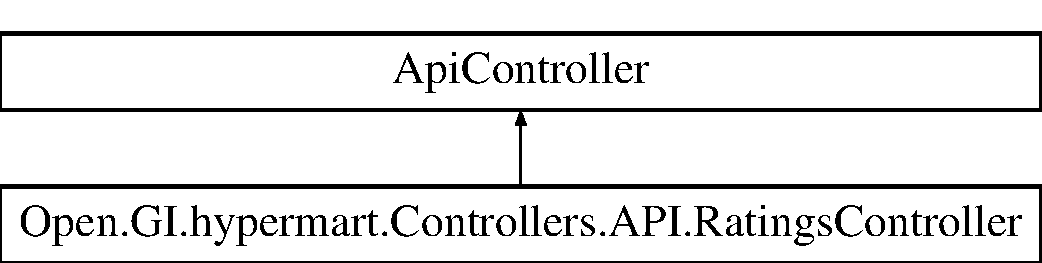
\includegraphics[height=2.000000cm]{class_open_1_1_g_i_1_1hypermart_1_1_controllers_1_1_a_p_i_1_1_ratings_controller}
\end{center}
\end{figure}
\subsection*{Public Member Functions}
\begin{DoxyCompactItemize}
\item 
I\+Enumerable$<$ String $>$ \textbf{ Get\+Available\+Rating\+Areas} ()
\begin{DoxyCompactList}\small\item\em Gets the rating areas. \end{DoxyCompactList}\item 
I\+Queryable$<$ \textbf{ Rating} $>$ \textbf{ Get\+Ratings} ()
\begin{DoxyCompactList}\small\item\em Gets the ratings. \end{DoxyCompactList}\item 
I\+Http\+Action\+Result \textbf{ Get\+Rating} (string id)
\begin{DoxyCompactList}\small\item\em Gets the rating. \end{DoxyCompactList}\item 
I\+Http\+Action\+Result \textbf{ Put\+Rating} (string id, \textbf{ Rating} rating)
\begin{DoxyCompactList}\small\item\em Puts the rating. \end{DoxyCompactList}\item 
I\+Http\+Action\+Result \textbf{ Post\+Rating} (\textbf{ Rating\+Information\+D\+TO} Rating\+To\+Add)
\begin{DoxyCompactList}\small\item\em Posts the rating. \end{DoxyCompactList}\item 
I\+Http\+Action\+Result \textbf{ Delete\+Rating} (string id)
\begin{DoxyCompactList}\small\item\em Deletes the rating. \end{DoxyCompactList}\end{DoxyCompactItemize}
\subsection*{Protected Member Functions}
\begin{DoxyCompactItemize}
\item 
override void \textbf{ Dispose} (bool disposing)
\begin{DoxyCompactList}\small\item\em Releases the unmanaged resources that are used by the object and, optionally, releases the managed resources. \end{DoxyCompactList}\end{DoxyCompactItemize}


\subsection{Detailed Description}
R\+E\+ST \doxyref{A\+PI}{p.}{namespace_open_1_1_g_i_1_1hypermart_1_1_controllers_1_1_a_p_i} layer for interacting with files. 

\begin{DoxySeeAlso}{See also}
System.\+Web.\+Http.\+Api\+Controller


\end{DoxySeeAlso}


Definition at line 21 of file Ratings\+Controller.\+cs.



\subsection{Member Function Documentation}
\mbox{\label{class_open_1_1_g_i_1_1hypermart_1_1_controllers_1_1_a_p_i_1_1_ratings_controller_aaf06db00da369f94fb3bffbc05a3491f}} 
\index{Open\+::\+G\+I\+::hypermart\+::\+Controllers\+::\+A\+P\+I\+::\+Ratings\+Controller@{Open\+::\+G\+I\+::hypermart\+::\+Controllers\+::\+A\+P\+I\+::\+Ratings\+Controller}!Delete\+Rating@{Delete\+Rating}}
\index{Delete\+Rating@{Delete\+Rating}!Open\+::\+G\+I\+::hypermart\+::\+Controllers\+::\+A\+P\+I\+::\+Ratings\+Controller@{Open\+::\+G\+I\+::hypermart\+::\+Controllers\+::\+A\+P\+I\+::\+Ratings\+Controller}}
\subsubsection{Delete\+Rating()}
{\footnotesize\ttfamily I\+Http\+Action\+Result Open.\+G\+I.\+hypermart.\+Controllers.\+A\+P\+I.\+Ratings\+Controller.\+Delete\+Rating (\begin{DoxyParamCaption}\item[{string}]{id }\end{DoxyParamCaption})}



Deletes the rating. 


\begin{DoxyParams}{Parameters}
{\em id} & The identifier.\\
\hline
\end{DoxyParams}
\begin{DoxyReturn}{Returns}

\end{DoxyReturn}


Definition at line 179 of file Ratings\+Controller.\+cs.

\mbox{\label{class_open_1_1_g_i_1_1hypermart_1_1_controllers_1_1_a_p_i_1_1_ratings_controller_abb9f3f53bdc7109192217e3dc99532a7}} 
\index{Open\+::\+G\+I\+::hypermart\+::\+Controllers\+::\+A\+P\+I\+::\+Ratings\+Controller@{Open\+::\+G\+I\+::hypermart\+::\+Controllers\+::\+A\+P\+I\+::\+Ratings\+Controller}!Dispose@{Dispose}}
\index{Dispose@{Dispose}!Open\+::\+G\+I\+::hypermart\+::\+Controllers\+::\+A\+P\+I\+::\+Ratings\+Controller@{Open\+::\+G\+I\+::hypermart\+::\+Controllers\+::\+A\+P\+I\+::\+Ratings\+Controller}}
\subsubsection{Dispose()}
{\footnotesize\ttfamily override void Open.\+G\+I.\+hypermart.\+Controllers.\+A\+P\+I.\+Ratings\+Controller.\+Dispose (\begin{DoxyParamCaption}\item[{bool}]{disposing }\end{DoxyParamCaption})\hspace{0.3cm}{\ttfamily [protected]}}



Releases the unmanaged resources that are used by the object and, optionally, releases the managed resources. 


\begin{DoxyParams}{Parameters}
{\em disposing} & true to release both managed and unmanaged resources; false to release only unmanaged resources.\\
\hline
\end{DoxyParams}


Definition at line 197 of file Ratings\+Controller.\+cs.

\mbox{\label{class_open_1_1_g_i_1_1hypermart_1_1_controllers_1_1_a_p_i_1_1_ratings_controller_a628d4db60f8c5ea8bbf03db08ee67178}} 
\index{Open\+::\+G\+I\+::hypermart\+::\+Controllers\+::\+A\+P\+I\+::\+Ratings\+Controller@{Open\+::\+G\+I\+::hypermart\+::\+Controllers\+::\+A\+P\+I\+::\+Ratings\+Controller}!Get\+Available\+Rating\+Areas@{Get\+Available\+Rating\+Areas}}
\index{Get\+Available\+Rating\+Areas@{Get\+Available\+Rating\+Areas}!Open\+::\+G\+I\+::hypermart\+::\+Controllers\+::\+A\+P\+I\+::\+Ratings\+Controller@{Open\+::\+G\+I\+::hypermart\+::\+Controllers\+::\+A\+P\+I\+::\+Ratings\+Controller}}
\subsubsection{Get\+Available\+Rating\+Areas()}
{\footnotesize\ttfamily I\+Enumerable$<$String$>$ Open.\+G\+I.\+hypermart.\+Controllers.\+A\+P\+I.\+Ratings\+Controller.\+Get\+Available\+Rating\+Areas (\begin{DoxyParamCaption}{ }\end{DoxyParamCaption})}



Gets the rating areas. 

\begin{DoxyReturn}{Returns}

\end{DoxyReturn}


Definition at line 29 of file Ratings\+Controller.\+cs.

\mbox{\label{class_open_1_1_g_i_1_1hypermart_1_1_controllers_1_1_a_p_i_1_1_ratings_controller_a79b77391187930a8c148fd4c3ae8e2f0}} 
\index{Open\+::\+G\+I\+::hypermart\+::\+Controllers\+::\+A\+P\+I\+::\+Ratings\+Controller@{Open\+::\+G\+I\+::hypermart\+::\+Controllers\+::\+A\+P\+I\+::\+Ratings\+Controller}!Get\+Rating@{Get\+Rating}}
\index{Get\+Rating@{Get\+Rating}!Open\+::\+G\+I\+::hypermart\+::\+Controllers\+::\+A\+P\+I\+::\+Ratings\+Controller@{Open\+::\+G\+I\+::hypermart\+::\+Controllers\+::\+A\+P\+I\+::\+Ratings\+Controller}}
\subsubsection{Get\+Rating()}
{\footnotesize\ttfamily I\+Http\+Action\+Result Open.\+G\+I.\+hypermart.\+Controllers.\+A\+P\+I.\+Ratings\+Controller.\+Get\+Rating (\begin{DoxyParamCaption}\item[{string}]{id }\end{DoxyParamCaption})}



Gets the rating. 


\begin{DoxyParams}{Parameters}
{\em id} & The identifier.\\
\hline
\end{DoxyParams}
\begin{DoxyReturn}{Returns}

\end{DoxyReturn}


Definition at line 54 of file Ratings\+Controller.\+cs.

\mbox{\label{class_open_1_1_g_i_1_1hypermart_1_1_controllers_1_1_a_p_i_1_1_ratings_controller_aa3ff04acf50d3bf4765f462c7fbdaf2b}} 
\index{Open\+::\+G\+I\+::hypermart\+::\+Controllers\+::\+A\+P\+I\+::\+Ratings\+Controller@{Open\+::\+G\+I\+::hypermart\+::\+Controllers\+::\+A\+P\+I\+::\+Ratings\+Controller}!Get\+Ratings@{Get\+Ratings}}
\index{Get\+Ratings@{Get\+Ratings}!Open\+::\+G\+I\+::hypermart\+::\+Controllers\+::\+A\+P\+I\+::\+Ratings\+Controller@{Open\+::\+G\+I\+::hypermart\+::\+Controllers\+::\+A\+P\+I\+::\+Ratings\+Controller}}
\subsubsection{Get\+Ratings()}
{\footnotesize\ttfamily I\+Queryable$<$\textbf{ Rating}$>$ Open.\+G\+I.\+hypermart.\+Controllers.\+A\+P\+I.\+Ratings\+Controller.\+Get\+Ratings (\begin{DoxyParamCaption}{ }\end{DoxyParamCaption})}



Gets the ratings. 

\begin{DoxyReturn}{Returns}

\end{DoxyReturn}


Definition at line 42 of file Ratings\+Controller.\+cs.

\mbox{\label{class_open_1_1_g_i_1_1hypermart_1_1_controllers_1_1_a_p_i_1_1_ratings_controller_a9d6b1b9e543bf0272c559a928a39541c}} 
\index{Open\+::\+G\+I\+::hypermart\+::\+Controllers\+::\+A\+P\+I\+::\+Ratings\+Controller@{Open\+::\+G\+I\+::hypermart\+::\+Controllers\+::\+A\+P\+I\+::\+Ratings\+Controller}!Post\+Rating@{Post\+Rating}}
\index{Post\+Rating@{Post\+Rating}!Open\+::\+G\+I\+::hypermart\+::\+Controllers\+::\+A\+P\+I\+::\+Ratings\+Controller@{Open\+::\+G\+I\+::hypermart\+::\+Controllers\+::\+A\+P\+I\+::\+Ratings\+Controller}}
\subsubsection{Post\+Rating()}
{\footnotesize\ttfamily I\+Http\+Action\+Result Open.\+G\+I.\+hypermart.\+Controllers.\+A\+P\+I.\+Ratings\+Controller.\+Post\+Rating (\begin{DoxyParamCaption}\item[{\textbf{ Rating\+Information\+D\+TO}}]{Rating\+To\+Add }\end{DoxyParamCaption})}



Posts the rating. 


\begin{DoxyParams}{Parameters}
{\em Rating\+To\+Add} & The rating.\\
\hline
\end{DoxyParams}
\begin{DoxyReturn}{Returns}

\end{DoxyReturn}


Definition at line 113 of file Ratings\+Controller.\+cs.

\mbox{\label{class_open_1_1_g_i_1_1hypermart_1_1_controllers_1_1_a_p_i_1_1_ratings_controller_a35f91cb72bc50655eae8e19780adb980}} 
\index{Open\+::\+G\+I\+::hypermart\+::\+Controllers\+::\+A\+P\+I\+::\+Ratings\+Controller@{Open\+::\+G\+I\+::hypermart\+::\+Controllers\+::\+A\+P\+I\+::\+Ratings\+Controller}!Put\+Rating@{Put\+Rating}}
\index{Put\+Rating@{Put\+Rating}!Open\+::\+G\+I\+::hypermart\+::\+Controllers\+::\+A\+P\+I\+::\+Ratings\+Controller@{Open\+::\+G\+I\+::hypermart\+::\+Controllers\+::\+A\+P\+I\+::\+Ratings\+Controller}}
\subsubsection{Put\+Rating()}
{\footnotesize\ttfamily I\+Http\+Action\+Result Open.\+G\+I.\+hypermart.\+Controllers.\+A\+P\+I.\+Ratings\+Controller.\+Put\+Rating (\begin{DoxyParamCaption}\item[{string}]{id,  }\item[{\textbf{ Rating}}]{rating }\end{DoxyParamCaption})}



Puts the rating. 


\begin{DoxyParams}{Parameters}
{\em id} & The identifier.\\
\hline
{\em rating} & The rating.\\
\hline
\end{DoxyParams}
\begin{DoxyReturn}{Returns}

\end{DoxyReturn}


Definition at line 73 of file Ratings\+Controller.\+cs.



The documentation for this class was generated from the following file\+:\begin{DoxyCompactItemize}
\item 
C\+:/\+Projects/\+App-\/\+Utility-\/\+Store/\+Open.\+G\+I.\+hypermart/\+Controllers/\+A\+P\+I/\textbf{ Ratings\+Controller.\+cs}\end{DoxyCompactItemize}

\hypertarget{class_open_1_1_g_i_1_1hypermart_1_1_route_config}{}\section{Open.\+G\+I.\+hypermart.\+Route\+Config Class Reference}
\label{class_open_1_1_g_i_1_1hypermart_1_1_route_config}\index{Open.\+G\+I.\+hypermart.\+Route\+Config@{Open.\+G\+I.\+hypermart.\+Route\+Config}}


M\+V\+C -\/ Route Registration  


\subsection*{Static Public Member Functions}
\begin{DoxyCompactItemize}
\item 
static void \hyperlink{class_open_1_1_g_i_1_1hypermart_1_1_route_config_a9b4bb82c10a972d509a88ad37cb1c783}{Register\+Routes} (Route\+Collection routes)
\begin{DoxyCompactList}\small\item\em Registers the routes. \end{DoxyCompactList}\end{DoxyCompactItemize}


\subsection{Detailed Description}
M\+V\+C -\/ Route Registration 



Definition at line 13 of file Route\+Config.\+cs.



\subsection{Member Function Documentation}
\hypertarget{class_open_1_1_g_i_1_1hypermart_1_1_route_config_a9b4bb82c10a972d509a88ad37cb1c783}{}\index{Open\+::\+G\+I\+::hypermart\+::\+Route\+Config@{Open\+::\+G\+I\+::hypermart\+::\+Route\+Config}!Register\+Routes@{Register\+Routes}}
\index{Register\+Routes@{Register\+Routes}!Open\+::\+G\+I\+::hypermart\+::\+Route\+Config@{Open\+::\+G\+I\+::hypermart\+::\+Route\+Config}}
\subsubsection[{Register\+Routes(\+Route\+Collection routes)}]{\setlength{\rightskip}{0pt plus 5cm}static void Open.\+G\+I.\+hypermart.\+Route\+Config.\+Register\+Routes (
\begin{DoxyParamCaption}
\item[{Route\+Collection}]{routes}
\end{DoxyParamCaption}
)\hspace{0.3cm}{\ttfamily [static]}}\label{class_open_1_1_g_i_1_1hypermart_1_1_route_config_a9b4bb82c10a972d509a88ad37cb1c783}


Registers the routes. 


\begin{DoxyParams}{Parameters}
{\em routes} & The routes.\\
\hline
\end{DoxyParams}


Definition at line 19 of file Route\+Config.\+cs.



The documentation for this class was generated from the following file\+:\begin{DoxyCompactItemize}
\item 
C\+:/\+Projects/\+App-\/\+Utility-\/\+Store/\+Open.\+G\+I.\+hypermart/\+App\+\_\+\+Start/\hyperlink{_route_config_8cs}{Route\+Config.\+cs}\end{DoxyCompactItemize}

\hypertarget{class_open_1_1_g_i_1_1hypermart_1_1_helpers_1_1_rss_action_result}{}\section{Open.\+G\+I.\+hypermart.\+Helpers.\+Rss\+Action\+Result Class Reference}
\label{class_open_1_1_g_i_1_1hypermart_1_1_helpers_1_1_rss_action_result}\index{Open.\+G\+I.\+hypermart.\+Helpers.\+Rss\+Action\+Result@{Open.\+G\+I.\+hypermart.\+Helpers.\+Rss\+Action\+Result}}


R\+SS Action Results  


Inheritance diagram for Open.\+G\+I.\+hypermart.\+Helpers.\+Rss\+Action\+Result\+:\begin{figure}[H]
\begin{center}
\leavevmode
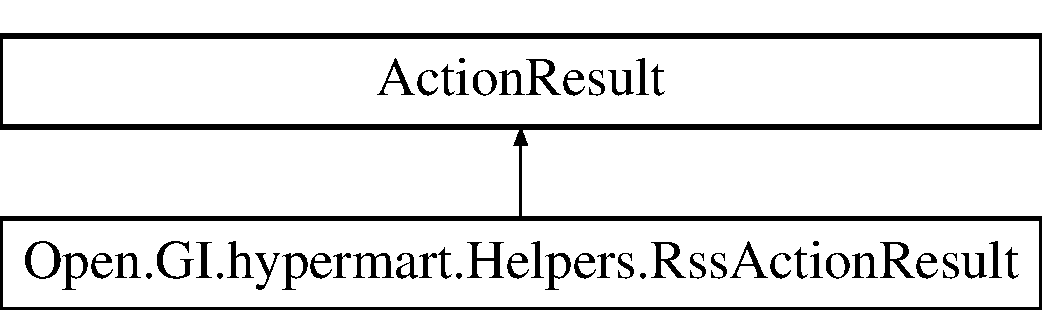
\includegraphics[height=2.000000cm]{class_open_1_1_g_i_1_1hypermart_1_1_helpers_1_1_rss_action_result}
\end{center}
\end{figure}
\subsection*{Public Member Functions}
\begin{DoxyCompactItemize}
\item 
override void \hyperlink{class_open_1_1_g_i_1_1hypermart_1_1_helpers_1_1_rss_action_result_a18ff30f679b2858b2d88a7dc267fd672}{Execute\+Result} (Controller\+Context context)
\begin{DoxyCompactList}\small\item\em Enables processing of the result of an action method by a custom type that inherits from the T\+:\+System.\+Web.\+Mvc.\+Action\+Result class. \end{DoxyCompactList}\end{DoxyCompactItemize}
\subsection*{Properties}
\begin{DoxyCompactItemize}
\item 
Syndication\+Feed \hyperlink{class_open_1_1_g_i_1_1hypermart_1_1_helpers_1_1_rss_action_result_a3b07cc4558b6a4863821fbedd9aa6888}{Feed}\hspace{0.3cm}{\ttfamily  \mbox{[}get, set\mbox{]}}
\begin{DoxyCompactList}\small\item\em Gets or sets the feed. \end{DoxyCompactList}\end{DoxyCompactItemize}


\subsection{Detailed Description}
R\+SS Action Results 

\begin{DoxySeeAlso}{See also}
System.\+Web.\+Mvc.\+Action\+Result


\end{DoxySeeAlso}


\subsection{Member Function Documentation}
\hypertarget{class_open_1_1_g_i_1_1hypermart_1_1_helpers_1_1_rss_action_result_a18ff30f679b2858b2d88a7dc267fd672}{}\label{class_open_1_1_g_i_1_1hypermart_1_1_helpers_1_1_rss_action_result_a18ff30f679b2858b2d88a7dc267fd672} 
\index{Open\+::\+G\+I\+::hypermart\+::\+Helpers\+::\+Rss\+Action\+Result@{Open\+::\+G\+I\+::hypermart\+::\+Helpers\+::\+Rss\+Action\+Result}!Execute\+Result@{Execute\+Result}}
\index{Execute\+Result@{Execute\+Result}!Open\+::\+G\+I\+::hypermart\+::\+Helpers\+::\+Rss\+Action\+Result@{Open\+::\+G\+I\+::hypermart\+::\+Helpers\+::\+Rss\+Action\+Result}}
\subsubsection{\texorpdfstring{Execute\+Result()}{ExecuteResult()}}
{\footnotesize\ttfamily override void Open.\+G\+I.\+hypermart.\+Helpers.\+Rss\+Action\+Result.\+Execute\+Result (\begin{DoxyParamCaption}\item[{Controller\+Context}]{context }\end{DoxyParamCaption})}



Enables processing of the result of an action method by a custom type that inherits from the T\+:\+System.\+Web.\+Mvc.\+Action\+Result class. 


\begin{DoxyParams}{Parameters}
{\em context} & The context in which the result is executed. The context information includes the controller, H\+T\+TP content, request context, and route data.\\
\hline
\end{DoxyParams}


\subsection{Property Documentation}
\hypertarget{class_open_1_1_g_i_1_1hypermart_1_1_helpers_1_1_rss_action_result_a3b07cc4558b6a4863821fbedd9aa6888}{}\label{class_open_1_1_g_i_1_1hypermart_1_1_helpers_1_1_rss_action_result_a3b07cc4558b6a4863821fbedd9aa6888} 
\index{Open\+::\+G\+I\+::hypermart\+::\+Helpers\+::\+Rss\+Action\+Result@{Open\+::\+G\+I\+::hypermart\+::\+Helpers\+::\+Rss\+Action\+Result}!Feed@{Feed}}
\index{Feed@{Feed}!Open\+::\+G\+I\+::hypermart\+::\+Helpers\+::\+Rss\+Action\+Result@{Open\+::\+G\+I\+::hypermart\+::\+Helpers\+::\+Rss\+Action\+Result}}
\subsubsection{\texorpdfstring{Feed}{Feed}}
{\footnotesize\ttfamily Syndication\+Feed Open.\+G\+I.\+hypermart.\+Helpers.\+Rss\+Action\+Result.\+Feed\hspace{0.3cm}{\ttfamily [get]}, {\ttfamily [set]}}



Gets or sets the feed. 

The feed. 

The documentation for this class was generated from the following file\+:\begin{DoxyCompactItemize}
\item 
C\+:/\+Projects/\+App-\/\+Utility-\/\+Store/\+Open.\+G\+I.\+hypermart/\+Helpers/\hyperlink{_rss_action_result_8cs}{Rss\+Action\+Result.\+cs}\end{DoxyCompactItemize}

\section{Open.\+G\+I.\+hypermart.\+Models.\+Screenshot Class Reference}
\label{class_open_1_1_g_i_1_1hypermart_1_1_models_1_1_screenshot}\index{Open.\+G\+I.\+hypermart.\+Models.\+Screenshot@{Open.\+G\+I.\+hypermart.\+Models.\+Screenshot}}


Screen Shot Model Class  


\subsection*{Properties}
\begin{DoxyCompactItemize}
\item 
int \textbf{ ID}\hspace{0.3cm}{\ttfamily  [get, set]}
\begin{DoxyCompactList}\small\item\em Gets or sets the identifier. \end{DoxyCompactList}\item 
byte [$\,$] \textbf{ Screen\+Shot1}\hspace{0.3cm}{\ttfamily  [get, set]}
\begin{DoxyCompactList}\small\item\em Gets or sets the screen shot1. \end{DoxyCompactList}\item 
int \textbf{ Product\+ID}\hspace{0.3cm}{\ttfamily  [get, set]}
\begin{DoxyCompactList}\small\item\em Gets or sets the product\+\_\+ identifier. \end{DoxyCompactList}\item 
\textbf{ Product} \textbf{ Product}\hspace{0.3cm}{\ttfamily  [get, set]}
\begin{DoxyCompactList}\small\item\em Gets or sets the product. \end{DoxyCompactList}\item 
virtual \textbf{ Product} \textbf{ Product}\hspace{0.3cm}{\ttfamily  [get, set]}
\end{DoxyCompactItemize}


\subsection{Detailed Description}
Screen Shot Model Class 



Definition at line 12 of file Screenshot.\+cs.



\subsection{Property Documentation}
\mbox{\label{class_open_1_1_g_i_1_1hypermart_1_1_models_1_1_screenshot_a7460fabffe75a362966595c8b86cdef2}} 
\index{Open\+::\+G\+I\+::hypermart\+::\+Models\+::\+Screenshot@{Open\+::\+G\+I\+::hypermart\+::\+Models\+::\+Screenshot}!ID@{ID}}
\index{ID@{ID}!Open\+::\+G\+I\+::hypermart\+::\+Models\+::\+Screenshot@{Open\+::\+G\+I\+::hypermart\+::\+Models\+::\+Screenshot}}
\subsubsection{ID}
{\footnotesize\ttfamily int Open.\+G\+I.\+hypermart.\+Models.\+Screenshot.\+ID\hspace{0.3cm}{\ttfamily [get]}, {\ttfamily [set]}}



Gets or sets the identifier. 

The identifier. 

Definition at line 20 of file Screenshot.\+cs.

\mbox{\label{class_open_1_1_g_i_1_1hypermart_1_1_models_1_1_screenshot_a8aed1d2289db7caefe8c7e14e0f5cc50}} 
\index{Open\+::\+G\+I\+::hypermart\+::\+Models\+::\+Screenshot@{Open\+::\+G\+I\+::hypermart\+::\+Models\+::\+Screenshot}!Product@{Product}}
\index{Product@{Product}!Open\+::\+G\+I\+::hypermart\+::\+Models\+::\+Screenshot@{Open\+::\+G\+I\+::hypermart\+::\+Models\+::\+Screenshot}}
\subsubsection{Product\hspace{0.1cm}{\footnotesize\ttfamily [1/2]}}
{\footnotesize\ttfamily virtual \textbf{ Product} Open.\+G\+I.\+hypermart.\+Models.\+Screenshot.\+Product\hspace{0.3cm}{\ttfamily [get]}, {\ttfamily [set]}}



Definition at line 21 of file Screenshot.\+cs.

\mbox{\label{class_open_1_1_g_i_1_1hypermart_1_1_models_1_1_screenshot_ae4e4b60e07136a6c4debe888426d6f6b}} 
\index{Open\+::\+G\+I\+::hypermart\+::\+Models\+::\+Screenshot@{Open\+::\+G\+I\+::hypermart\+::\+Models\+::\+Screenshot}!Product@{Product}}
\index{Product@{Product}!Open\+::\+G\+I\+::hypermart\+::\+Models\+::\+Screenshot@{Open\+::\+G\+I\+::hypermart\+::\+Models\+::\+Screenshot}}
\subsubsection{Product\hspace{0.1cm}{\footnotesize\ttfamily [2/2]}}
{\footnotesize\ttfamily \textbf{ Product} Open.\+G\+I.\+hypermart.\+Models.\+Screenshot.\+Product\hspace{0.3cm}{\ttfamily [get]}, {\ttfamily [set]}}



Gets or sets the product. 

The product. 

Definition at line 46 of file Screenshot.\+cs.

\mbox{\label{class_open_1_1_g_i_1_1hypermart_1_1_models_1_1_screenshot_ad381abf51bb0ebb1c2566c70df11c05a}} 
\index{Open\+::\+G\+I\+::hypermart\+::\+Models\+::\+Screenshot@{Open\+::\+G\+I\+::hypermart\+::\+Models\+::\+Screenshot}!Product\+ID@{Product\+ID}}
\index{Product\+ID@{Product\+ID}!Open\+::\+G\+I\+::hypermart\+::\+Models\+::\+Screenshot@{Open\+::\+G\+I\+::hypermart\+::\+Models\+::\+Screenshot}}
\subsubsection{Product\+ID}
{\footnotesize\ttfamily int Open.\+G\+I.\+hypermart.\+Models.\+Screenshot.\+Product\+ID\hspace{0.3cm}{\ttfamily [get]}, {\ttfamily [set]}}



Gets or sets the product\+\_\+ identifier. 

The product\+\_\+ identifier. 

Definition at line 38 of file Screenshot.\+cs.

\mbox{\label{class_open_1_1_g_i_1_1hypermart_1_1_models_1_1_screenshot_a435ca1863d66de2de497d603585610d8}} 
\index{Open\+::\+G\+I\+::hypermart\+::\+Models\+::\+Screenshot@{Open\+::\+G\+I\+::hypermart\+::\+Models\+::\+Screenshot}!Screen\+Shot1@{Screen\+Shot1}}
\index{Screen\+Shot1@{Screen\+Shot1}!Open\+::\+G\+I\+::hypermart\+::\+Models\+::\+Screenshot@{Open\+::\+G\+I\+::hypermart\+::\+Models\+::\+Screenshot}}
\subsubsection{Screen\+Shot1}
{\footnotesize\ttfamily byte [$\,$] Open.\+G\+I.\+hypermart.\+Models.\+Screenshot.\+Screen\+Shot1\hspace{0.3cm}{\ttfamily [get]}, {\ttfamily [set]}}



Gets or sets the screen shot1. 

The screen shot1. 

Definition at line 30 of file Screenshot.\+cs.



The documentation for this class was generated from the following file\+:\begin{DoxyCompactItemize}
\item 
C\+:/\+Projects/\+App-\/\+Utility-\/\+Store/\+Open.\+G\+I.\+hypermart/\+Models/\textbf{ Screenshot.\+cs}\end{DoxyCompactItemize}

\section{Open.\+G\+I.\+hypermart.\+Docs.\+Data\+Transformation\+Objects.\+Screen\+Shot\+D\+TO Class Reference}
\label{class_open_1_1_g_i_1_1hypermart_1_1_docs_1_1_data_transformation_objects_1_1_screen_shot_d_t_o}\index{Open.\+G\+I.\+hypermart.\+Docs.\+Data\+Transformation\+Objects.\+Screen\+Shot\+D\+TO@{Open.\+G\+I.\+hypermart.\+Docs.\+Data\+Transformation\+Objects.\+Screen\+Shot\+D\+TO}}


Screen\+Shot D\+TO  


\subsection*{Public Member Functions}
\begin{DoxyCompactItemize}
\item 
\textbf{ Screen\+Shot\+D\+TO} (\textbf{ Screenshot} screenshot)
\begin{DoxyCompactList}\small\item\em Screen\+Shot D\+TO Constructor \end{DoxyCompactList}\end{DoxyCompactItemize}
\subsection*{Properties}
\begin{DoxyCompactItemize}
\item 
int \textbf{ ID}\hspace{0.3cm}{\ttfamily  [get, set]}
\item 
byte [$\,$] \textbf{ Screen\+Shot1}\hspace{0.3cm}{\ttfamily  [get, set]}
\end{DoxyCompactItemize}


\subsection{Detailed Description}
Screen\+Shot D\+TO 



Definition at line 12 of file Screen\+Shot\+D\+T\+O.\+cs.



\subsection{Constructor \& Destructor Documentation}
\mbox{\label{class_open_1_1_g_i_1_1hypermart_1_1_docs_1_1_data_transformation_objects_1_1_screen_shot_d_t_o_a1d16d059ad949737184bd5b8061d036d}} 
\index{Open\+::\+G\+I\+::hypermart\+::\+Docs\+::\+Data\+Transformation\+Objects\+::\+Screen\+Shot\+D\+TO@{Open\+::\+G\+I\+::hypermart\+::\+Docs\+::\+Data\+Transformation\+Objects\+::\+Screen\+Shot\+D\+TO}!Screen\+Shot\+D\+TO@{Screen\+Shot\+D\+TO}}
\index{Screen\+Shot\+D\+TO@{Screen\+Shot\+D\+TO}!Open\+::\+G\+I\+::hypermart\+::\+Docs\+::\+Data\+Transformation\+Objects\+::\+Screen\+Shot\+D\+TO@{Open\+::\+G\+I\+::hypermart\+::\+Docs\+::\+Data\+Transformation\+Objects\+::\+Screen\+Shot\+D\+TO}}
\subsubsection{Screen\+Shot\+D\+T\+O()}
{\footnotesize\ttfamily Open.\+G\+I.\+hypermart.\+Docs.\+Data\+Transformation\+Objects.\+Screen\+Shot\+D\+T\+O.\+Screen\+Shot\+D\+TO (\begin{DoxyParamCaption}\item[{\textbf{ Screenshot}}]{screenshot }\end{DoxyParamCaption})}



Screen\+Shot D\+TO Constructor 


\begin{DoxyParams}{Parameters}
{\em screenshot} & \\
\hline
\end{DoxyParams}


Definition at line 18 of file Screen\+Shot\+D\+T\+O.\+cs.



\subsection{Property Documentation}
\mbox{\label{class_open_1_1_g_i_1_1hypermart_1_1_docs_1_1_data_transformation_objects_1_1_screen_shot_d_t_o_ae97d094ea2ba7b786d2fd171b12cc3e6}} 
\index{Open\+::\+G\+I\+::hypermart\+::\+Docs\+::\+Data\+Transformation\+Objects\+::\+Screen\+Shot\+D\+TO@{Open\+::\+G\+I\+::hypermart\+::\+Docs\+::\+Data\+Transformation\+Objects\+::\+Screen\+Shot\+D\+TO}!ID@{ID}}
\index{ID@{ID}!Open\+::\+G\+I\+::hypermart\+::\+Docs\+::\+Data\+Transformation\+Objects\+::\+Screen\+Shot\+D\+TO@{Open\+::\+G\+I\+::hypermart\+::\+Docs\+::\+Data\+Transformation\+Objects\+::\+Screen\+Shot\+D\+TO}}
\subsubsection{ID}
{\footnotesize\ttfamily int Open.\+G\+I.\+hypermart.\+Docs.\+Data\+Transformation\+Objects.\+Screen\+Shot\+D\+T\+O.\+ID\hspace{0.3cm}{\ttfamily [get]}, {\ttfamily [set]}}







Definition at line 26 of file Screen\+Shot\+D\+T\+O.\+cs.

\mbox{\label{class_open_1_1_g_i_1_1hypermart_1_1_docs_1_1_data_transformation_objects_1_1_screen_shot_d_t_o_af8a951a853f5107194edf4f3fe9168a8}} 
\index{Open\+::\+G\+I\+::hypermart\+::\+Docs\+::\+Data\+Transformation\+Objects\+::\+Screen\+Shot\+D\+TO@{Open\+::\+G\+I\+::hypermart\+::\+Docs\+::\+Data\+Transformation\+Objects\+::\+Screen\+Shot\+D\+TO}!Screen\+Shot1@{Screen\+Shot1}}
\index{Screen\+Shot1@{Screen\+Shot1}!Open\+::\+G\+I\+::hypermart\+::\+Docs\+::\+Data\+Transformation\+Objects\+::\+Screen\+Shot\+D\+TO@{Open\+::\+G\+I\+::hypermart\+::\+Docs\+::\+Data\+Transformation\+Objects\+::\+Screen\+Shot\+D\+TO}}
\subsubsection{Screen\+Shot1}
{\footnotesize\ttfamily byte [$\,$] Open.\+G\+I.\+hypermart.\+Docs.\+Data\+Transformation\+Objects.\+Screen\+Shot\+D\+T\+O.\+Screen\+Shot1\hspace{0.3cm}{\ttfamily [get]}, {\ttfamily [set]}}







Definition at line 30 of file Screen\+Shot\+D\+T\+O.\+cs.



The documentation for this class was generated from the following file\+:\begin{DoxyCompactItemize}
\item 
C\+:/\+Projects/\+App-\/\+Utility-\/\+Store/\+Open.\+G\+I.\+hypermart/\+Docs/\+Data\+Transformation\+Objects/\textbf{ Screen\+Shot\+D\+T\+O.\+cs}\end{DoxyCompactItemize}

\section{Open.\+G\+I.\+hypermart.\+Controllers.\+A\+P\+I.\+Screenshots\+Controller Class Reference}
\label{class_open_1_1_g_i_1_1hypermart_1_1_controllers_1_1_a_p_i_1_1_screenshots_controller}\index{Open.\+G\+I.\+hypermart.\+Controllers.\+A\+P\+I.\+Screenshots\+Controller@{Open.\+G\+I.\+hypermart.\+Controllers.\+A\+P\+I.\+Screenshots\+Controller}}


R\+E\+ST \doxyref{A\+PI}{p.}{namespace_open_1_1_g_i_1_1hypermart_1_1_controllers_1_1_a_p_i} layer for interacting with screenshots.  


Inheritance diagram for Open.\+G\+I.\+hypermart.\+Controllers.\+A\+P\+I.\+Screenshots\+Controller\+:\begin{figure}[H]
\begin{center}
\leavevmode
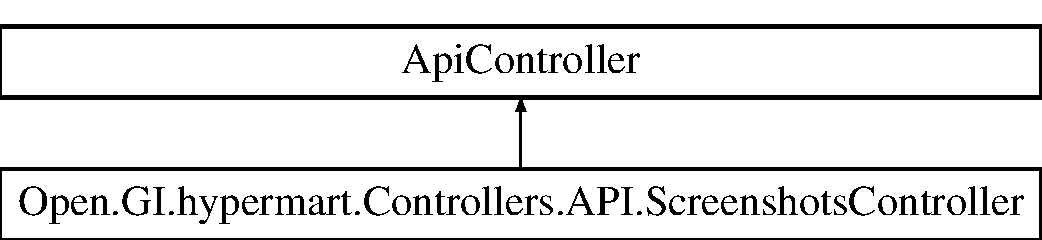
\includegraphics[height=2.000000cm]{class_open_1_1_g_i_1_1hypermart_1_1_controllers_1_1_a_p_i_1_1_screenshots_controller}
\end{center}
\end{figure}
\subsection*{Public Member Functions}
\begin{DoxyCompactItemize}
\item 
\textbf{ Screenshots\+Controller} ()
\begin{DoxyCompactList}\small\item\em Initializes a new instance of the \doxyref{Screenshots\+Controller}{p.}{class_open_1_1_g_i_1_1hypermart_1_1_controllers_1_1_a_p_i_1_1_screenshots_controller} class. \end{DoxyCompactList}\item 
I\+Enumerable$<$ \textbf{ Screen\+Shot\+D\+TO} $>$ \textbf{ Get\+Screenshots} ()
\begin{DoxyCompactList}\small\item\em Gets the screenshots. \end{DoxyCompactList}\item 
I\+Http\+Action\+Result \textbf{ Get\+Screenshot} (int id)
\begin{DoxyCompactList}\small\item\em Gets the screenshot. \end{DoxyCompactList}\item 
I\+Http\+Action\+Result \textbf{ Put\+Screenshot} (int id, \textbf{ Screenshot} screenshot)
\begin{DoxyCompactList}\small\item\em Puts the screenshot. \end{DoxyCompactList}\item 
I\+Http\+Action\+Result \textbf{ Post\+Screenshot} (\textbf{ Screen\+Shot\+D\+TO} screenshot)
\begin{DoxyCompactList}\small\item\em Posts the screenshot. \end{DoxyCompactList}\item 
I\+Http\+Action\+Result \textbf{ Delete\+Screenshot} (int id)
\begin{DoxyCompactList}\small\item\em Deletes the screenshot. \end{DoxyCompactList}\end{DoxyCompactItemize}
\subsection*{Protected Member Functions}
\begin{DoxyCompactItemize}
\item 
override void \textbf{ Dispose} (bool disposing)
\begin{DoxyCompactList}\small\item\em Releases the unmanaged resources that are used by the object and, optionally, releases the managed resources. \end{DoxyCompactList}\end{DoxyCompactItemize}


\subsection{Detailed Description}
R\+E\+ST \doxyref{A\+PI}{p.}{namespace_open_1_1_g_i_1_1hypermart_1_1_controllers_1_1_a_p_i} layer for interacting with screenshots. 

\begin{DoxySeeAlso}{See also}
System.\+Web.\+Http.\+Api\+Controller


\end{DoxySeeAlso}


Definition at line 21 of file Screenshots\+Controller.\+cs.



\subsection{Constructor \& Destructor Documentation}
\mbox{\label{class_open_1_1_g_i_1_1hypermart_1_1_controllers_1_1_a_p_i_1_1_screenshots_controller_a38315fc7ad90feab2c072d48de02b602}} 
\index{Open\+::\+G\+I\+::hypermart\+::\+Controllers\+::\+A\+P\+I\+::\+Screenshots\+Controller@{Open\+::\+G\+I\+::hypermart\+::\+Controllers\+::\+A\+P\+I\+::\+Screenshots\+Controller}!Screenshots\+Controller@{Screenshots\+Controller}}
\index{Screenshots\+Controller@{Screenshots\+Controller}!Open\+::\+G\+I\+::hypermart\+::\+Controllers\+::\+A\+P\+I\+::\+Screenshots\+Controller@{Open\+::\+G\+I\+::hypermart\+::\+Controllers\+::\+A\+P\+I\+::\+Screenshots\+Controller}}
\subsubsection{Screenshots\+Controller()}
{\footnotesize\ttfamily Open.\+G\+I.\+hypermart.\+Controllers.\+A\+P\+I.\+Screenshots\+Controller.\+Screenshots\+Controller (\begin{DoxyParamCaption}{ }\end{DoxyParamCaption})}



Initializes a new instance of the \doxyref{Screenshots\+Controller}{p.}{class_open_1_1_g_i_1_1hypermart_1_1_controllers_1_1_a_p_i_1_1_screenshots_controller} class. 



Definition at line 27 of file Screenshots\+Controller.\+cs.



\subsection{Member Function Documentation}
\mbox{\label{class_open_1_1_g_i_1_1hypermart_1_1_controllers_1_1_a_p_i_1_1_screenshots_controller_a85094c9aa969d9d3fc2a746847eef6e8}} 
\index{Open\+::\+G\+I\+::hypermart\+::\+Controllers\+::\+A\+P\+I\+::\+Screenshots\+Controller@{Open\+::\+G\+I\+::hypermart\+::\+Controllers\+::\+A\+P\+I\+::\+Screenshots\+Controller}!Delete\+Screenshot@{Delete\+Screenshot}}
\index{Delete\+Screenshot@{Delete\+Screenshot}!Open\+::\+G\+I\+::hypermart\+::\+Controllers\+::\+A\+P\+I\+::\+Screenshots\+Controller@{Open\+::\+G\+I\+::hypermart\+::\+Controllers\+::\+A\+P\+I\+::\+Screenshots\+Controller}}
\subsubsection{Delete\+Screenshot()}
{\footnotesize\ttfamily I\+Http\+Action\+Result Open.\+G\+I.\+hypermart.\+Controllers.\+A\+P\+I.\+Screenshots\+Controller.\+Delete\+Screenshot (\begin{DoxyParamCaption}\item[{int}]{id }\end{DoxyParamCaption})}



Deletes the screenshot. 


\begin{DoxyParams}{Parameters}
{\em id} & The identifier.\\
\hline
\end{DoxyParams}
\begin{DoxyReturn}{Returns}

\end{DoxyReturn}


Definition at line 130 of file Screenshots\+Controller.\+cs.

\mbox{\label{class_open_1_1_g_i_1_1hypermart_1_1_controllers_1_1_a_p_i_1_1_screenshots_controller_a63f56d0cc46aa71b08e2360e242af42d}} 
\index{Open\+::\+G\+I\+::hypermart\+::\+Controllers\+::\+A\+P\+I\+::\+Screenshots\+Controller@{Open\+::\+G\+I\+::hypermart\+::\+Controllers\+::\+A\+P\+I\+::\+Screenshots\+Controller}!Dispose@{Dispose}}
\index{Dispose@{Dispose}!Open\+::\+G\+I\+::hypermart\+::\+Controllers\+::\+A\+P\+I\+::\+Screenshots\+Controller@{Open\+::\+G\+I\+::hypermart\+::\+Controllers\+::\+A\+P\+I\+::\+Screenshots\+Controller}}
\subsubsection{Dispose()}
{\footnotesize\ttfamily override void Open.\+G\+I.\+hypermart.\+Controllers.\+A\+P\+I.\+Screenshots\+Controller.\+Dispose (\begin{DoxyParamCaption}\item[{bool}]{disposing }\end{DoxyParamCaption})\hspace{0.3cm}{\ttfamily [protected]}}



Releases the unmanaged resources that are used by the object and, optionally, releases the managed resources. 


\begin{DoxyParams}{Parameters}
{\em disposing} & true to release both managed and unmanaged resources; false to release only unmanaged resources.\\
\hline
\end{DoxyParams}


Definition at line 147 of file Screenshots\+Controller.\+cs.

\mbox{\label{class_open_1_1_g_i_1_1hypermart_1_1_controllers_1_1_a_p_i_1_1_screenshots_controller_abfe715c661c5a7a53ac5a382ff24b354}} 
\index{Open\+::\+G\+I\+::hypermart\+::\+Controllers\+::\+A\+P\+I\+::\+Screenshots\+Controller@{Open\+::\+G\+I\+::hypermart\+::\+Controllers\+::\+A\+P\+I\+::\+Screenshots\+Controller}!Get\+Screenshot@{Get\+Screenshot}}
\index{Get\+Screenshot@{Get\+Screenshot}!Open\+::\+G\+I\+::hypermart\+::\+Controllers\+::\+A\+P\+I\+::\+Screenshots\+Controller@{Open\+::\+G\+I\+::hypermart\+::\+Controllers\+::\+A\+P\+I\+::\+Screenshots\+Controller}}
\subsubsection{Get\+Screenshot()}
{\footnotesize\ttfamily I\+Http\+Action\+Result Open.\+G\+I.\+hypermart.\+Controllers.\+A\+P\+I.\+Screenshots\+Controller.\+Get\+Screenshot (\begin{DoxyParamCaption}\item[{int}]{id }\end{DoxyParamCaption})}



Gets the screenshot. 


\begin{DoxyParams}{Parameters}
{\em id} & The identifier.\\
\hline
\end{DoxyParams}
\begin{DoxyReturn}{Returns}

\end{DoxyReturn}


Definition at line 51 of file Screenshots\+Controller.\+cs.

\mbox{\label{class_open_1_1_g_i_1_1hypermart_1_1_controllers_1_1_a_p_i_1_1_screenshots_controller_a59d05cd470e6721699f0234f99c9a213}} 
\index{Open\+::\+G\+I\+::hypermart\+::\+Controllers\+::\+A\+P\+I\+::\+Screenshots\+Controller@{Open\+::\+G\+I\+::hypermart\+::\+Controllers\+::\+A\+P\+I\+::\+Screenshots\+Controller}!Get\+Screenshots@{Get\+Screenshots}}
\index{Get\+Screenshots@{Get\+Screenshots}!Open\+::\+G\+I\+::hypermart\+::\+Controllers\+::\+A\+P\+I\+::\+Screenshots\+Controller@{Open\+::\+G\+I\+::hypermart\+::\+Controllers\+::\+A\+P\+I\+::\+Screenshots\+Controller}}
\subsubsection{Get\+Screenshots()}
{\footnotesize\ttfamily I\+Enumerable$<$\textbf{ Screen\+Shot\+D\+TO}$>$ Open.\+G\+I.\+hypermart.\+Controllers.\+A\+P\+I.\+Screenshots\+Controller.\+Get\+Screenshots (\begin{DoxyParamCaption}{ }\end{DoxyParamCaption})}



Gets the screenshots. 

\begin{DoxyReturn}{Returns}

\end{DoxyReturn}


Definition at line 37 of file Screenshots\+Controller.\+cs.

\mbox{\label{class_open_1_1_g_i_1_1hypermart_1_1_controllers_1_1_a_p_i_1_1_screenshots_controller_a31b7e3814b2ea1fde97b28a76b6315db}} 
\index{Open\+::\+G\+I\+::hypermart\+::\+Controllers\+::\+A\+P\+I\+::\+Screenshots\+Controller@{Open\+::\+G\+I\+::hypermart\+::\+Controllers\+::\+A\+P\+I\+::\+Screenshots\+Controller}!Post\+Screenshot@{Post\+Screenshot}}
\index{Post\+Screenshot@{Post\+Screenshot}!Open\+::\+G\+I\+::hypermart\+::\+Controllers\+::\+A\+P\+I\+::\+Screenshots\+Controller@{Open\+::\+G\+I\+::hypermart\+::\+Controllers\+::\+A\+P\+I\+::\+Screenshots\+Controller}}
\subsubsection{Post\+Screenshot()}
{\footnotesize\ttfamily I\+Http\+Action\+Result Open.\+G\+I.\+hypermart.\+Controllers.\+A\+P\+I.\+Screenshots\+Controller.\+Post\+Screenshot (\begin{DoxyParamCaption}\item[{\textbf{ Screen\+Shot\+D\+TO}}]{screenshot }\end{DoxyParamCaption})}



Posts the screenshot. 


\begin{DoxyParams}{Parameters}
{\em screenshot} & The screenshot.\\
\hline
\end{DoxyParams}
\begin{DoxyReturn}{Returns}

\end{DoxyReturn}


Definition at line 110 of file Screenshots\+Controller.\+cs.

\mbox{\label{class_open_1_1_g_i_1_1hypermart_1_1_controllers_1_1_a_p_i_1_1_screenshots_controller_a5b53a659a1cf98b2e2866bc9415f69bd}} 
\index{Open\+::\+G\+I\+::hypermart\+::\+Controllers\+::\+A\+P\+I\+::\+Screenshots\+Controller@{Open\+::\+G\+I\+::hypermart\+::\+Controllers\+::\+A\+P\+I\+::\+Screenshots\+Controller}!Put\+Screenshot@{Put\+Screenshot}}
\index{Put\+Screenshot@{Put\+Screenshot}!Open\+::\+G\+I\+::hypermart\+::\+Controllers\+::\+A\+P\+I\+::\+Screenshots\+Controller@{Open\+::\+G\+I\+::hypermart\+::\+Controllers\+::\+A\+P\+I\+::\+Screenshots\+Controller}}
\subsubsection{Put\+Screenshot()}
{\footnotesize\ttfamily I\+Http\+Action\+Result Open.\+G\+I.\+hypermart.\+Controllers.\+A\+P\+I.\+Screenshots\+Controller.\+Put\+Screenshot (\begin{DoxyParamCaption}\item[{int}]{id,  }\item[{\textbf{ Screenshot}}]{screenshot }\end{DoxyParamCaption})}



Puts the screenshot. 


\begin{DoxyParams}{Parameters}
{\em id} & The identifier.\\
\hline
{\em screenshot} & The screenshot.\\
\hline
\end{DoxyParams}
\begin{DoxyReturn}{Returns}

\end{DoxyReturn}


Definition at line 70 of file Screenshots\+Controller.\+cs.



The documentation for this class was generated from the following file\+:\begin{DoxyCompactItemize}
\item 
C\+:/\+Projects/\+App-\/\+Utility-\/\+Store/\+Open.\+G\+I.\+hypermart/\+Controllers/\+A\+P\+I/\textbf{ Screenshots\+Controller.\+cs}\end{DoxyCompactItemize}

\section{Open.\+G\+I.\+hypermart.\+Helpers.\+Search Class Reference}
\label{class_open_1_1_g_i_1_1hypermart_1_1_helpers_1_1_search}\index{Open.\+G\+I.\+hypermart.\+Helpers.\+Search@{Open.\+G\+I.\+hypermart.\+Helpers.\+Search}}


Lucene \doxyref{Search}{p.}{class_open_1_1_g_i_1_1hypermart_1_1_helpers_1_1_search} -\/ searching the store using Lucene  




\subsection{Detailed Description}
Lucene \doxyref{Search}{p.}{class_open_1_1_g_i_1_1hypermart_1_1_helpers_1_1_search} -\/ searching the store using Lucene 



Definition at line 13 of file Search.\+cs.



The documentation for this class was generated from the following file\+:\begin{DoxyCompactItemize}
\item 
C\+:/\+Projects/\+App-\/\+Utility-\/\+Store/\+Open.\+G\+I.\+hypermart/\+Helpers/\textbf{ Search.\+cs}\end{DoxyCompactItemize}

\hypertarget{class_open_1_1_g_i_1_1hypermart_1_1_controllers_1_1_search_controller}{}\section{Open.\+G\+I.\+hypermart.\+Controllers.\+Search\+Controller Class Reference}
\label{class_open_1_1_g_i_1_1hypermart_1_1_controllers_1_1_search_controller}\index{Open.\+G\+I.\+hypermart.\+Controllers.\+Search\+Controller@{Open.\+G\+I.\+hypermart.\+Controllers.\+Search\+Controller}}


Performs searches against the Product metadata (possibly also against the user database) -\/ to be decided  


Inheritance diagram for Open.\+G\+I.\+hypermart.\+Controllers.\+Search\+Controller\+:\begin{figure}[H]
\begin{center}
\leavevmode
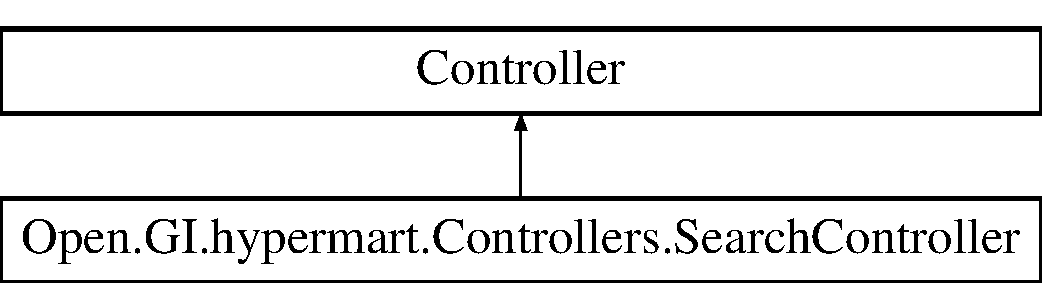
\includegraphics[height=2.000000cm]{class_open_1_1_g_i_1_1hypermart_1_1_controllers_1_1_search_controller}
\end{center}
\end{figure}
\subsection*{Public Member Functions}
\begin{DoxyCompactItemize}
\item 
\hyperlink{class_open_1_1_g_i_1_1hypermart_1_1_controllers_1_1_search_controller_a91d14626e4163f0af2ccc84b135a8949}{Search\+Controller} (\hyperlink{interface_open_1_1_g_i_1_1hypermart_1_1_d_a_l_1_1_i_hypermart_context}{I\+Hypermart\+Context} \hyperlink{class_open_1_1_g_i_1_1hypermart_1_1_controllers_1_1_search_controller_ac0b1c112b3b87593f00d2fd7fe7f1a07}{db})
\begin{DoxyCompactList}\small\item\em Controller -\/ passing in contrext \end{DoxyCompactList}\item 
\hyperlink{class_open_1_1_g_i_1_1hypermart_1_1_controllers_1_1_search_controller_a8bd1641a18d5720e47a17e91e8957977}{Search\+Controller} ()
\begin{DoxyCompactList}\small\item\em Standard installer for Search Controller \end{DoxyCompactList}\item 
Action\+Result \hyperlink{class_open_1_1_g_i_1_1hypermart_1_1_controllers_1_1_search_controller_a92174a9db0c7ca485afd0c513ad8f66d}{Index} (string Search\+Term)
\begin{DoxyCompactList}\small\item\em Indexes the specified search term. (performs a search, returns a list of results) \end{DoxyCompactList}\end{DoxyCompactItemize}
\subsection*{Properties}
\begin{DoxyCompactItemize}
\item 
\hyperlink{interface_open_1_1_g_i_1_1hypermart_1_1_d_a_l_1_1_i_hypermart_context}{I\+Hypermart\+Context} \hyperlink{class_open_1_1_g_i_1_1hypermart_1_1_controllers_1_1_search_controller_ac0b1c112b3b87593f00d2fd7fe7f1a07}{db}\hspace{0.3cm}{\ttfamily  \mbox{[}get, set\mbox{]}}
\begin{DoxyCompactList}\small\item\em \hyperlink{namespace_open_1_1_g_i_1_1hypermart_1_1_d_a_l}{D\+AL} \end{DoxyCompactList}\end{DoxyCompactItemize}


\subsection{Detailed Description}
Performs searches against the Product metadata (possibly also against the user database) -\/ to be decided 

\begin{DoxySeeAlso}{See also}
System.\+Web.\+Mvc.\+Controller


\end{DoxySeeAlso}


\subsection{Constructor \& Destructor Documentation}
\hypertarget{class_open_1_1_g_i_1_1hypermart_1_1_controllers_1_1_search_controller_a91d14626e4163f0af2ccc84b135a8949}{}\label{class_open_1_1_g_i_1_1hypermart_1_1_controllers_1_1_search_controller_a91d14626e4163f0af2ccc84b135a8949} 
\index{Open\+::\+G\+I\+::hypermart\+::\+Controllers\+::\+Search\+Controller@{Open\+::\+G\+I\+::hypermart\+::\+Controllers\+::\+Search\+Controller}!Search\+Controller@{Search\+Controller}}
\index{Search\+Controller@{Search\+Controller}!Open\+::\+G\+I\+::hypermart\+::\+Controllers\+::\+Search\+Controller@{Open\+::\+G\+I\+::hypermart\+::\+Controllers\+::\+Search\+Controller}}
\subsubsection{\texorpdfstring{Search\+Controller()}{SearchController()}\hspace{0.1cm}{\footnotesize\ttfamily [1/2]}}
{\footnotesize\ttfamily Open.\+G\+I.\+hypermart.\+Controllers.\+Search\+Controller.\+Search\+Controller (\begin{DoxyParamCaption}\item[{\hyperlink{interface_open_1_1_g_i_1_1hypermart_1_1_d_a_l_1_1_i_hypermart_context}{I\+Hypermart\+Context}}]{db }\end{DoxyParamCaption})}



Controller -\/ passing in contrext 


\begin{DoxyParams}{Parameters}
{\em db} & \\
\hline
\end{DoxyParams}
\hypertarget{class_open_1_1_g_i_1_1hypermart_1_1_controllers_1_1_search_controller_a8bd1641a18d5720e47a17e91e8957977}{}\label{class_open_1_1_g_i_1_1hypermart_1_1_controllers_1_1_search_controller_a8bd1641a18d5720e47a17e91e8957977} 
\index{Open\+::\+G\+I\+::hypermart\+::\+Controllers\+::\+Search\+Controller@{Open\+::\+G\+I\+::hypermart\+::\+Controllers\+::\+Search\+Controller}!Search\+Controller@{Search\+Controller}}
\index{Search\+Controller@{Search\+Controller}!Open\+::\+G\+I\+::hypermart\+::\+Controllers\+::\+Search\+Controller@{Open\+::\+G\+I\+::hypermart\+::\+Controllers\+::\+Search\+Controller}}
\subsubsection{\texorpdfstring{Search\+Controller()}{SearchController()}\hspace{0.1cm}{\footnotesize\ttfamily [2/2]}}
{\footnotesize\ttfamily Open.\+G\+I.\+hypermart.\+Controllers.\+Search\+Controller.\+Search\+Controller (\begin{DoxyParamCaption}{ }\end{DoxyParamCaption})}



Standard installer for Search Controller 



\subsection{Member Function Documentation}
\hypertarget{class_open_1_1_g_i_1_1hypermart_1_1_controllers_1_1_search_controller_a92174a9db0c7ca485afd0c513ad8f66d}{}\label{class_open_1_1_g_i_1_1hypermart_1_1_controllers_1_1_search_controller_a92174a9db0c7ca485afd0c513ad8f66d} 
\index{Open\+::\+G\+I\+::hypermart\+::\+Controllers\+::\+Search\+Controller@{Open\+::\+G\+I\+::hypermart\+::\+Controllers\+::\+Search\+Controller}!Index@{Index}}
\index{Index@{Index}!Open\+::\+G\+I\+::hypermart\+::\+Controllers\+::\+Search\+Controller@{Open\+::\+G\+I\+::hypermart\+::\+Controllers\+::\+Search\+Controller}}
\subsubsection{\texorpdfstring{Index()}{Index()}}
{\footnotesize\ttfamily Action\+Result Open.\+G\+I.\+hypermart.\+Controllers.\+Search\+Controller.\+Index (\begin{DoxyParamCaption}\item[{string}]{Search\+Term }\end{DoxyParamCaption})}



Indexes the specified search term. (performs a search, returns a list of results) 


\begin{DoxyParams}{Parameters}
{\em Search\+Term} & The search term.\\
\hline
\end{DoxyParams}
\begin{DoxyReturn}{Returns}

\end{DoxyReturn}


\subsection{Property Documentation}
\hypertarget{class_open_1_1_g_i_1_1hypermart_1_1_controllers_1_1_search_controller_ac0b1c112b3b87593f00d2fd7fe7f1a07}{}\label{class_open_1_1_g_i_1_1hypermart_1_1_controllers_1_1_search_controller_ac0b1c112b3b87593f00d2fd7fe7f1a07} 
\index{Open\+::\+G\+I\+::hypermart\+::\+Controllers\+::\+Search\+Controller@{Open\+::\+G\+I\+::hypermart\+::\+Controllers\+::\+Search\+Controller}!db@{db}}
\index{db@{db}!Open\+::\+G\+I\+::hypermart\+::\+Controllers\+::\+Search\+Controller@{Open\+::\+G\+I\+::hypermart\+::\+Controllers\+::\+Search\+Controller}}
\subsubsection{\texorpdfstring{db}{db}}
{\footnotesize\ttfamily \hyperlink{interface_open_1_1_g_i_1_1hypermart_1_1_d_a_l_1_1_i_hypermart_context}{I\+Hypermart\+Context} Open.\+G\+I.\+hypermart.\+Controllers.\+Search\+Controller.\+db\hspace{0.3cm}{\ttfamily [get]}, {\ttfamily [set]}}



\hyperlink{namespace_open_1_1_g_i_1_1hypermart_1_1_d_a_l}{D\+AL} 



The documentation for this class was generated from the following file\+:\begin{DoxyCompactItemize}
\item 
C\+:/\+Projects/\+App-\/\+Utility-\/\+Store/\+Open.\+G\+I.\+hypermart/\+Controllers/\hyperlink{_search_controller_8cs}{Search\+Controller.\+cs}\end{DoxyCompactItemize}

\hypertarget{class_open_1_1_g_i_1_1hypermart_1_1_models_1_1_service}{}\section{Open.\+G\+I.\+hypermart.\+Models.\+Service Class Reference}
\label{class_open_1_1_g_i_1_1hypermart_1_1_models_1_1_service}\index{Open.\+G\+I.\+hypermart.\+Models.\+Service@{Open.\+G\+I.\+hypermart.\+Models.\+Service}}


Class which decribes a \hyperlink{class_open_1_1_g_i_1_1hypermart_1_1_models_1_1_service}{Service}, providing an O\+Auth Access token to allow secured access.  


\subsection*{Properties}
\begin{DoxyCompactItemize}
\item 
string \hyperlink{class_open_1_1_g_i_1_1hypermart_1_1_models_1_1_service_a13b20f7866ea05fde10c7e4541e07aee}{Name}\hspace{0.3cm}{\ttfamily  \mbox{[}get, set\mbox{]}}
\begin{DoxyCompactList}\small\item\em Gets or sets the name of the script \end{DoxyCompactList}\item 
\hyperlink{class_open_1_1_g_i_1_1hypermart_1_1_models_1_1_user}{User} \hyperlink{class_open_1_1_g_i_1_1hypermart_1_1_models_1_1_service_ab0719ac31980c99022040f5887ad332d}{User\+Name}\hspace{0.3cm}{\ttfamily  \mbox{[}get, set\mbox{]}}
\begin{DoxyCompactList}\small\item\em Gets or sets the name of the user responsible for this script. \end{DoxyCompactList}\end{DoxyCompactItemize}


\subsection{Detailed Description}
Class which decribes a \hyperlink{class_open_1_1_g_i_1_1hypermart_1_1_models_1_1_service}{Service}, providing an O\+Auth Access token to allow secured access. 



\subsection{Property Documentation}
\hypertarget{class_open_1_1_g_i_1_1hypermart_1_1_models_1_1_service_a13b20f7866ea05fde10c7e4541e07aee}{}\label{class_open_1_1_g_i_1_1hypermart_1_1_models_1_1_service_a13b20f7866ea05fde10c7e4541e07aee} 
\index{Open\+::\+G\+I\+::hypermart\+::\+Models\+::\+Service@{Open\+::\+G\+I\+::hypermart\+::\+Models\+::\+Service}!Name@{Name}}
\index{Name@{Name}!Open\+::\+G\+I\+::hypermart\+::\+Models\+::\+Service@{Open\+::\+G\+I\+::hypermart\+::\+Models\+::\+Service}}
\subsubsection{\texorpdfstring{Name}{Name}}
{\footnotesize\ttfamily string Open.\+G\+I.\+hypermart.\+Models.\+Service.\+Name\hspace{0.3cm}{\ttfamily [get]}, {\ttfamily [set]}}



Gets or sets the name of the script 

The name. \hypertarget{class_open_1_1_g_i_1_1hypermart_1_1_models_1_1_service_ab0719ac31980c99022040f5887ad332d}{}\label{class_open_1_1_g_i_1_1hypermart_1_1_models_1_1_service_ab0719ac31980c99022040f5887ad332d} 
\index{Open\+::\+G\+I\+::hypermart\+::\+Models\+::\+Service@{Open\+::\+G\+I\+::hypermart\+::\+Models\+::\+Service}!User\+Name@{User\+Name}}
\index{User\+Name@{User\+Name}!Open\+::\+G\+I\+::hypermart\+::\+Models\+::\+Service@{Open\+::\+G\+I\+::hypermart\+::\+Models\+::\+Service}}
\subsubsection{\texorpdfstring{User\+Name}{UserName}}
{\footnotesize\ttfamily \hyperlink{class_open_1_1_g_i_1_1hypermart_1_1_models_1_1_user}{User} Open.\+G\+I.\+hypermart.\+Models.\+Service.\+User\+Name\hspace{0.3cm}{\ttfamily [get]}, {\ttfamily [set]}}



Gets or sets the name of the user responsible for this script. 

The name of the user. 

The documentation for this class was generated from the following file\+:\begin{DoxyCompactItemize}
\item 
C\+:/\+Projects/\+App-\/\+Utility-\/\+Store/\+Open.\+G\+I.\+hypermart/\+Models/\hyperlink{_service_8cs}{Service.\+cs}\end{DoxyCompactItemize}

\hypertarget{class_open_1_1_g_i_1_1hypermart_1_1_areas_1_1_help_page_1_1_model_descriptions_1_1_simple_type_model_description}{}\section{Open.\+G\+I.\+hypermart.\+Areas.\+Help\+Page.\+Model\+Descriptions.\+Simple\+Type\+Model\+Description Class Reference}
\label{class_open_1_1_g_i_1_1hypermart_1_1_areas_1_1_help_page_1_1_model_descriptions_1_1_simple_type_model_description}\index{Open.\+G\+I.\+hypermart.\+Areas.\+Help\+Page.\+Model\+Descriptions.\+Simple\+Type\+Model\+Description@{Open.\+G\+I.\+hypermart.\+Areas.\+Help\+Page.\+Model\+Descriptions.\+Simple\+Type\+Model\+Description}}


 


Inheritance diagram for Open.\+G\+I.\+hypermart.\+Areas.\+Help\+Page.\+Model\+Descriptions.\+Simple\+Type\+Model\+Description\+:\begin{figure}[H]
\begin{center}
\leavevmode
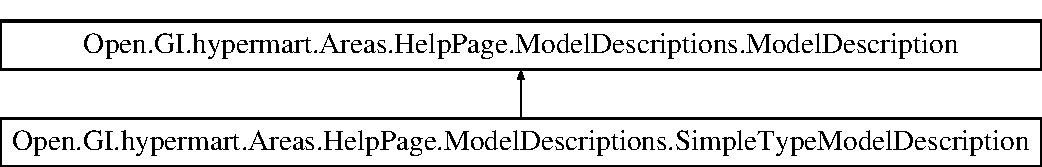
\includegraphics[height=2.000000cm]{class_open_1_1_g_i_1_1hypermart_1_1_areas_1_1_help_page_1_1_model_descriptions_1_1_simple_type_model_description}
\end{center}
\end{figure}
\subsection*{Additional Inherited Members}


\subsection{Detailed Description}


\begin{DoxySeeAlso}{See also}
\hyperlink{class_open_1_1_g_i_1_1hypermart_1_1_areas_1_1_help_page_1_1_model_descriptions_1_1_model_description}{Open.\+G\+I.\+hypermart.\+Areas.\+Help\+Page.\+Model\+Descriptions.\+Model\+Description}


\end{DoxySeeAlso}


Definition at line 7 of file Simple\+Type\+Model\+Description.\+cs.



The documentation for this class was generated from the following file\+:\begin{DoxyCompactItemize}
\item 
C\+:/\+Projects/\+App-\/\+Utility-\/\+Store/\+Open.\+G\+I.\+hypermart/\+Areas/\+Help\+Page/\+Model\+Descriptions/\hyperlink{_simple_type_model_description_8cs}{Simple\+Type\+Model\+Description.\+cs}\end{DoxyCompactItemize}

\hypertarget{class_open_1_1_g_i_1_1hypermart_1_1_startup}{}\section{Open.\+G\+I.\+hypermart.\+Startup Class Reference}
\label{class_open_1_1_g_i_1_1hypermart_1_1_startup}\index{Open.\+G\+I.\+hypermart.\+Startup@{Open.\+G\+I.\+hypermart.\+Startup}}


Class that will eventually form the kernel for the O\+Auth Authentication system for Scripts.  


\subsection*{Public Member Functions}
\begin{DoxyCompactItemize}
\item 
void \hyperlink{class_open_1_1_g_i_1_1hypermart_1_1_startup_a92c0680464156e20b32f17ef38e08a83}{Configuration} (I\+App\+Builder app)
\begin{DoxyCompactList}\small\item\em Configurations the specified application. \end{DoxyCompactList}\end{DoxyCompactItemize}


\subsection{Detailed Description}
Class that will eventually form the kernel for the O\+Auth Authentication system for Scripts. 



\subsection{Member Function Documentation}
\hypertarget{class_open_1_1_g_i_1_1hypermart_1_1_startup_a92c0680464156e20b32f17ef38e08a83}{}\label{class_open_1_1_g_i_1_1hypermart_1_1_startup_a92c0680464156e20b32f17ef38e08a83} 
\index{Open\+::\+G\+I\+::hypermart\+::\+Startup@{Open\+::\+G\+I\+::hypermart\+::\+Startup}!Configuration@{Configuration}}
\index{Configuration@{Configuration}!Open\+::\+G\+I\+::hypermart\+::\+Startup@{Open\+::\+G\+I\+::hypermart\+::\+Startup}}
\subsubsection{\texorpdfstring{Configuration()}{Configuration()}}
{\footnotesize\ttfamily void Open.\+G\+I.\+hypermart.\+Startup.\+Configuration (\begin{DoxyParamCaption}\item[{I\+App\+Builder}]{app }\end{DoxyParamCaption})}



Configurations the specified application. 


\begin{DoxyParams}{Parameters}
{\em app} & The application.\\
\hline
\end{DoxyParams}


The documentation for this class was generated from the following file\+:\begin{DoxyCompactItemize}
\item 
C\+:/\+Projects/\+App-\/\+Utility-\/\+Store/\+Open.\+G\+I.\+hypermart/\hyperlink{_startup_8cs}{Startup.\+cs}\end{DoxyCompactItemize}

\section{Open.\+G\+I.\+hypermart.\+Status Class Reference}
\label{class_open_1_1_g_i_1_1hypermart_1_1_status}\index{Open.\+G\+I.\+hypermart.\+Status@{Open.\+G\+I.\+hypermart.\+Status}}


Summary description for \doxyref{Status}{p.}{class_open_1_1_g_i_1_1hypermart_1_1_status}  


Inheritance diagram for Open.\+G\+I.\+hypermart.\+Status\+:\begin{figure}[H]
\begin{center}
\leavevmode
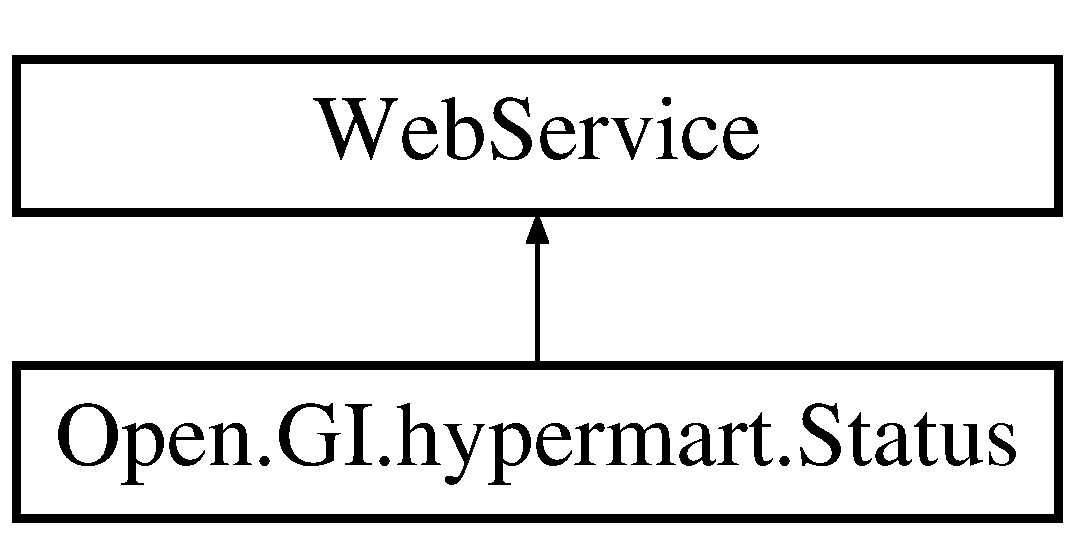
\includegraphics[height=2.000000cm]{class_open_1_1_g_i_1_1hypermart_1_1_status}
\end{center}
\end{figure}
\subsection*{Public Member Functions}
\begin{DoxyCompactItemize}
\item 
string \textbf{ Hello\+World} ()
\begin{DoxyCompactList}\small\item\em This is the Hello World method. \end{DoxyCompactList}\end{DoxyCompactItemize}


\subsection{Detailed Description}
Summary description for \doxyref{Status}{p.}{class_open_1_1_g_i_1_1hypermart_1_1_status} 



Definition at line 17 of file Status.\+asmx.\+cs.



\subsection{Member Function Documentation}
\mbox{\label{class_open_1_1_g_i_1_1hypermart_1_1_status_a73a11d6869226091bd66017995dfabef}} 
\index{Open\+::\+G\+I\+::hypermart\+::\+Status@{Open\+::\+G\+I\+::hypermart\+::\+Status}!Hello\+World@{Hello\+World}}
\index{Hello\+World@{Hello\+World}!Open\+::\+G\+I\+::hypermart\+::\+Status@{Open\+::\+G\+I\+::hypermart\+::\+Status}}
\subsubsection{Hello\+World()}
{\footnotesize\ttfamily string Open.\+G\+I.\+hypermart.\+Status.\+Hello\+World (\begin{DoxyParamCaption}{ }\end{DoxyParamCaption})}



This is the Hello World method. 

\begin{DoxyReturn}{Returns}

\end{DoxyReturn}


Definition at line 25 of file Status.\+asmx.\+cs.



The documentation for this class was generated from the following file\+:\begin{DoxyCompactItemize}
\item 
C\+:/\+Projects/\+App-\/\+Utility-\/\+Store/\+Open.\+G\+I.\+hypermart/\textbf{ Status.\+asmx.\+cs}\end{DoxyCompactItemize}

\hypertarget{class_open_1_1_g_i_1_1hypermart_1_1_attributes_1_1_store_attribute}{}\section{Open.\+G\+I.\+hypermart.\+Attributes.\+Store\+Attribute Class Reference}
\label{class_open_1_1_g_i_1_1hypermart_1_1_attributes_1_1_store_attribute}\index{Open.\+G\+I.\+hypermart.\+Attributes.\+Store\+Attribute@{Open.\+G\+I.\+hypermart.\+Attributes.\+Store\+Attribute}}


Custom attribute, assignable to an assembly that can store information connecting this .N\+ET assembly to a Hypermarket Store entry.  


Inheritance diagram for Open.\+G\+I.\+hypermart.\+Attributes.\+Store\+Attribute\+:\begin{figure}[H]
\begin{center}
\leavevmode
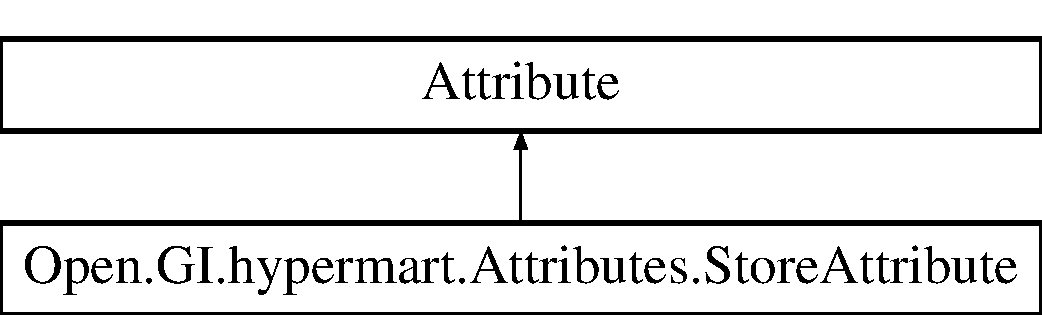
\includegraphics[height=2.000000cm]{class_open_1_1_g_i_1_1hypermart_1_1_attributes_1_1_store_attribute}
\end{center}
\end{figure}
\subsection*{Public Member Functions}
\begin{DoxyCompactItemize}
\item 
\hyperlink{class_open_1_1_g_i_1_1hypermart_1_1_attributes_1_1_store_attribute_a127c005e38f149d6c12fda40173ec7f1}{Store\+Attribute} (int \hyperlink{class_open_1_1_g_i_1_1hypermart_1_1_attributes_1_1_store_attribute_acf647c6eece8333d1d8d817474d5776d}{Product\+ID}, int \hyperlink{class_open_1_1_g_i_1_1hypermart_1_1_attributes_1_1_store_attribute_aa321f5e2ab58ed219e952f1e8036fcfa}{File\+ID})
\begin{DoxyCompactList}\small\item\em Initializes a new instance of the \hyperlink{class_open_1_1_g_i_1_1hypermart_1_1_attributes_1_1_store_attribute}{Store\+Attribute} class. \end{DoxyCompactList}\end{DoxyCompactItemize}
\subsection*{Properties}
\begin{DoxyCompactItemize}
\item 
int \hyperlink{class_open_1_1_g_i_1_1hypermart_1_1_attributes_1_1_store_attribute_acf647c6eece8333d1d8d817474d5776d}{Product\+ID}\hspace{0.3cm}{\ttfamily  \mbox{[}get, set\mbox{]}}
\begin{DoxyCompactList}\small\item\em Gets or sets the product identifier. \end{DoxyCompactList}\item 
int \hyperlink{class_open_1_1_g_i_1_1hypermart_1_1_attributes_1_1_store_attribute_aa321f5e2ab58ed219e952f1e8036fcfa}{File\+ID}\hspace{0.3cm}{\ttfamily  \mbox{[}get, set\mbox{]}}
\begin{DoxyCompactList}\small\item\em Gets or sets the file identifier. \end{DoxyCompactList}\end{DoxyCompactItemize}


\subsection{Detailed Description}
Custom attribute, assignable to an assembly that can store information connecting this .N\+ET assembly to a Hypermarket Store entry. 

\begin{DoxySeeAlso}{See also}
System.\+Attribute


\end{DoxySeeAlso}


\subsection{Constructor \& Destructor Documentation}
\hypertarget{class_open_1_1_g_i_1_1hypermart_1_1_attributes_1_1_store_attribute_a127c005e38f149d6c12fda40173ec7f1}{}\label{class_open_1_1_g_i_1_1hypermart_1_1_attributes_1_1_store_attribute_a127c005e38f149d6c12fda40173ec7f1} 
\index{Open\+::\+G\+I\+::hypermart\+::\+Attributes\+::\+Store\+Attribute@{Open\+::\+G\+I\+::hypermart\+::\+Attributes\+::\+Store\+Attribute}!Store\+Attribute@{Store\+Attribute}}
\index{Store\+Attribute@{Store\+Attribute}!Open\+::\+G\+I\+::hypermart\+::\+Attributes\+::\+Store\+Attribute@{Open\+::\+G\+I\+::hypermart\+::\+Attributes\+::\+Store\+Attribute}}
\subsubsection{\texorpdfstring{Store\+Attribute()}{StoreAttribute()}}
{\footnotesize\ttfamily Open.\+G\+I.\+hypermart.\+Attributes.\+Store\+Attribute.\+Store\+Attribute (\begin{DoxyParamCaption}\item[{int}]{Product\+ID,  }\item[{int}]{File\+ID }\end{DoxyParamCaption})}



Initializes a new instance of the \hyperlink{class_open_1_1_g_i_1_1hypermart_1_1_attributes_1_1_store_attribute}{Store\+Attribute} class. 


\begin{DoxyParams}{Parameters}
{\em Product\+ID} & The product identifier.\\
\hline
{\em File\+ID} & The file identifier.\\
\hline
\end{DoxyParams}


\subsection{Property Documentation}
\hypertarget{class_open_1_1_g_i_1_1hypermart_1_1_attributes_1_1_store_attribute_aa321f5e2ab58ed219e952f1e8036fcfa}{}\label{class_open_1_1_g_i_1_1hypermart_1_1_attributes_1_1_store_attribute_aa321f5e2ab58ed219e952f1e8036fcfa} 
\index{Open\+::\+G\+I\+::hypermart\+::\+Attributes\+::\+Store\+Attribute@{Open\+::\+G\+I\+::hypermart\+::\+Attributes\+::\+Store\+Attribute}!File\+ID@{File\+ID}}
\index{File\+ID@{File\+ID}!Open\+::\+G\+I\+::hypermart\+::\+Attributes\+::\+Store\+Attribute@{Open\+::\+G\+I\+::hypermart\+::\+Attributes\+::\+Store\+Attribute}}
\subsubsection{\texorpdfstring{File\+ID}{FileID}}
{\footnotesize\ttfamily int Open.\+G\+I.\+hypermart.\+Attributes.\+Store\+Attribute.\+File\+ID\hspace{0.3cm}{\ttfamily [get]}, {\ttfamily [set]}}



Gets or sets the file identifier. 

The file identifier. \hypertarget{class_open_1_1_g_i_1_1hypermart_1_1_attributes_1_1_store_attribute_acf647c6eece8333d1d8d817474d5776d}{}\label{class_open_1_1_g_i_1_1hypermart_1_1_attributes_1_1_store_attribute_acf647c6eece8333d1d8d817474d5776d} 
\index{Open\+::\+G\+I\+::hypermart\+::\+Attributes\+::\+Store\+Attribute@{Open\+::\+G\+I\+::hypermart\+::\+Attributes\+::\+Store\+Attribute}!Product\+ID@{Product\+ID}}
\index{Product\+ID@{Product\+ID}!Open\+::\+G\+I\+::hypermart\+::\+Attributes\+::\+Store\+Attribute@{Open\+::\+G\+I\+::hypermart\+::\+Attributes\+::\+Store\+Attribute}}
\subsubsection{\texorpdfstring{Product\+ID}{ProductID}}
{\footnotesize\ttfamily int Open.\+G\+I.\+hypermart.\+Attributes.\+Store\+Attribute.\+Product\+ID\hspace{0.3cm}{\ttfamily [get]}, {\ttfamily [set]}}



Gets or sets the product identifier. 

The product identifier. 

The documentation for this class was generated from the following file\+:\begin{DoxyCompactItemize}
\item 
C\+:/\+Projects/\+App-\/\+Utility-\/\+Store/\+Open.\+G\+I.\+hypermart/\+Attributes/\hyperlink{_store_attribute_8cs}{Store\+Attribute.\+cs}\end{DoxyCompactItemize}

\section{Open.\+G\+I.\+hypermart.\+Controllers.\+Store\+Content\+Controller Class Reference}
\label{class_open_1_1_g_i_1_1hypermart_1_1_controllers_1_1_store_content_controller}\index{Open.\+G\+I.\+hypermart.\+Controllers.\+Store\+Content\+Controller@{Open.\+G\+I.\+hypermart.\+Controllers.\+Store\+Content\+Controller}}


This is the Open\+GI \doxyref{A\+PI}{p.}{namespace_open_1_1_g_i_1_1hypermart_1_1_controllers_1_1_a_p_i} layer for interacting with the Store(\+Ading content etc). Some of the calls here relating to updates and creation will require a session token.  


Inheritance diagram for Open.\+G\+I.\+hypermart.\+Controllers.\+Store\+Content\+Controller\+:\begin{figure}[H]
\begin{center}
\leavevmode
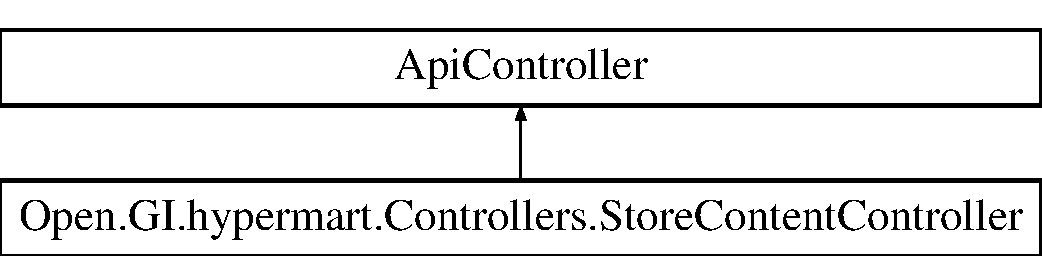
\includegraphics[height=2.000000cm]{class_open_1_1_g_i_1_1hypermart_1_1_controllers_1_1_store_content_controller}
\end{center}
\end{figure}
\subsection*{Public Member Functions}
\begin{DoxyCompactItemize}
\item 
\textbf{ Store\+Content\+Controller} ()
\begin{DoxyCompactList}\small\item\em Initializes a new instance of the \doxyref{Store\+Content\+Controller}{p.}{class_open_1_1_g_i_1_1hypermart_1_1_controllers_1_1_store_content_controller} class. \end{DoxyCompactList}\item 
\textbf{ Store\+Content\+Controller} (\textbf{ I\+Hypermart\+Context} db\+Context)
\begin{DoxyCompactList}\small\item\em Initializes a new instance of the \doxyref{Store\+Content\+Controller}{p.}{class_open_1_1_g_i_1_1hypermart_1_1_controllers_1_1_store_content_controller} class. \end{DoxyCompactList}\item 
I\+Queryable$<$ \textbf{ Product\+D\+TO} $>$ \textbf{ Get\+All\+Products} ()
\begin{DoxyCompactList}\small\item\em Gets all products. \end{DoxyCompactList}\item 
\textbf{ Product\+D\+TO} \textbf{ Get\+Product} (int id)
\begin{DoxyCompactList}\small\item\em Gets a product. \end{DoxyCompactList}\item 
\textbf{ Product\+D\+TO} \textbf{ Post\+Product} (\textbf{ Product} item\+To\+Add)
\begin{DoxyCompactList}\small\item\em Create a New Product \end{DoxyCompactList}\item 
bool \textbf{ Delete\+Product} (\textbf{ Product} product\+To\+Delete)
\begin{DoxyCompactList}\small\item\em Deletes the product. \end{DoxyCompactList}\item 
void \textbf{ Delete\+Product} (int Product\+ID)
\begin{DoxyCompactList}\small\item\em Deletes the product. \end{DoxyCompactList}\item 
List$<$ \textbf{ File\+D\+TO} $>$ \textbf{ Get\+Files} (int id)
\begin{DoxyCompactList}\small\item\em Gets all files for a product. \end{DoxyCompactList}\item 
\textbf{ File\+D\+TO} \textbf{ Post\+Product\+File} (int Product\+ID, \textbf{ Open.\+G\+I.\+hypermart.\+Models.\+File} File\+To\+Add)
\begin{DoxyCompactList}\small\item\em Posts the product file. \end{DoxyCompactList}\item 
\textbf{ File\+D\+TO} \textbf{ Add\+File} (int Product\+ID, \textbf{ Open.\+G\+I.\+hypermart.\+Models.\+File} File\+To\+Add)
\begin{DoxyCompactList}\small\item\em Add A File to a product \end{DoxyCompactList}\item 
void \textbf{ Add\+Screen\+Shot} (int Product\+ID)
\begin{DoxyCompactList}\small\item\em Add a Screenshot to an Product \end{DoxyCompactList}\item 
void \textbf{ Post\+Ratings} (\textbf{ Rating\+Information\+D\+TO} Rating\+To\+Add)
\begin{DoxyCompactList}\small\item\em Create a New Product Rating \end{DoxyCompactList}\end{DoxyCompactItemize}


\subsection{Detailed Description}
This is the Open\+GI \doxyref{A\+PI}{p.}{namespace_open_1_1_g_i_1_1hypermart_1_1_controllers_1_1_a_p_i} layer for interacting with the Store(\+Ading content etc). Some of the calls here relating to updates and creation will require a session token. 



Definition at line 21 of file Store\+Content\+Controller.\+cs.



\subsection{Constructor \& Destructor Documentation}
\mbox{\label{class_open_1_1_g_i_1_1hypermart_1_1_controllers_1_1_store_content_controller_a01bad24ca04f869ec58d136ff35b2d13}} 
\index{Open\+::\+G\+I\+::hypermart\+::\+Controllers\+::\+Store\+Content\+Controller@{Open\+::\+G\+I\+::hypermart\+::\+Controllers\+::\+Store\+Content\+Controller}!Store\+Content\+Controller@{Store\+Content\+Controller}}
\index{Store\+Content\+Controller@{Store\+Content\+Controller}!Open\+::\+G\+I\+::hypermart\+::\+Controllers\+::\+Store\+Content\+Controller@{Open\+::\+G\+I\+::hypermart\+::\+Controllers\+::\+Store\+Content\+Controller}}
\subsubsection{Store\+Content\+Controller()\hspace{0.1cm}{\footnotesize\ttfamily [1/2]}}
{\footnotesize\ttfamily Open.\+G\+I.\+hypermart.\+Controllers.\+Store\+Content\+Controller.\+Store\+Content\+Controller (\begin{DoxyParamCaption}{ }\end{DoxyParamCaption})}



Initializes a new instance of the \doxyref{Store\+Content\+Controller}{p.}{class_open_1_1_g_i_1_1hypermart_1_1_controllers_1_1_store_content_controller} class. 



Definition at line 27 of file Store\+Content\+Controller.\+cs.

\mbox{\label{class_open_1_1_g_i_1_1hypermart_1_1_controllers_1_1_store_content_controller_ad8b3b3f13892bbb028eb21b7e240d7e2}} 
\index{Open\+::\+G\+I\+::hypermart\+::\+Controllers\+::\+Store\+Content\+Controller@{Open\+::\+G\+I\+::hypermart\+::\+Controllers\+::\+Store\+Content\+Controller}!Store\+Content\+Controller@{Store\+Content\+Controller}}
\index{Store\+Content\+Controller@{Store\+Content\+Controller}!Open\+::\+G\+I\+::hypermart\+::\+Controllers\+::\+Store\+Content\+Controller@{Open\+::\+G\+I\+::hypermart\+::\+Controllers\+::\+Store\+Content\+Controller}}
\subsubsection{Store\+Content\+Controller()\hspace{0.1cm}{\footnotesize\ttfamily [2/2]}}
{\footnotesize\ttfamily Open.\+G\+I.\+hypermart.\+Controllers.\+Store\+Content\+Controller.\+Store\+Content\+Controller (\begin{DoxyParamCaption}\item[{\textbf{ I\+Hypermart\+Context}}]{db\+Context }\end{DoxyParamCaption})}



Initializes a new instance of the \doxyref{Store\+Content\+Controller}{p.}{class_open_1_1_g_i_1_1hypermart_1_1_controllers_1_1_store_content_controller} class. 


\begin{DoxyParams}{Parameters}
{\em db\+Context} & The database context.\\
\hline
\end{DoxyParams}


Definition at line 36 of file Store\+Content\+Controller.\+cs.



\subsection{Member Function Documentation}
\mbox{\label{class_open_1_1_g_i_1_1hypermart_1_1_controllers_1_1_store_content_controller_a36a438b2ab2cbb1d937b6a4c5bd8b17d}} 
\index{Open\+::\+G\+I\+::hypermart\+::\+Controllers\+::\+Store\+Content\+Controller@{Open\+::\+G\+I\+::hypermart\+::\+Controllers\+::\+Store\+Content\+Controller}!Add\+File@{Add\+File}}
\index{Add\+File@{Add\+File}!Open\+::\+G\+I\+::hypermart\+::\+Controllers\+::\+Store\+Content\+Controller@{Open\+::\+G\+I\+::hypermart\+::\+Controllers\+::\+Store\+Content\+Controller}}
\subsubsection{Add\+File()}
{\footnotesize\ttfamily \textbf{ File\+D\+TO} Open.\+G\+I.\+hypermart.\+Controllers.\+Store\+Content\+Controller.\+Add\+File (\begin{DoxyParamCaption}\item[{int}]{Product\+ID,  }\item[{\textbf{ Open.\+G\+I.\+hypermart.\+Models.\+File}}]{File\+To\+Add }\end{DoxyParamCaption})}



Add A File to a product 


\begin{DoxyParams}{Parameters}
{\em Product\+ID} & \\
\hline
{\em File\+To\+Add} & \\
\hline
\end{DoxyParams}
\begin{DoxyReturn}{Returns}

\end{DoxyReturn}


Definition at line 211 of file Store\+Content\+Controller.\+cs.

\mbox{\label{class_open_1_1_g_i_1_1hypermart_1_1_controllers_1_1_store_content_controller_a7c5b861d456ae7b592165634a07c6738}} 
\index{Open\+::\+G\+I\+::hypermart\+::\+Controllers\+::\+Store\+Content\+Controller@{Open\+::\+G\+I\+::hypermart\+::\+Controllers\+::\+Store\+Content\+Controller}!Add\+Screen\+Shot@{Add\+Screen\+Shot}}
\index{Add\+Screen\+Shot@{Add\+Screen\+Shot}!Open\+::\+G\+I\+::hypermart\+::\+Controllers\+::\+Store\+Content\+Controller@{Open\+::\+G\+I\+::hypermart\+::\+Controllers\+::\+Store\+Content\+Controller}}
\subsubsection{Add\+Screen\+Shot()}
{\footnotesize\ttfamily void Open.\+G\+I.\+hypermart.\+Controllers.\+Store\+Content\+Controller.\+Add\+Screen\+Shot (\begin{DoxyParamCaption}\item[{int}]{Product\+ID }\end{DoxyParamCaption})}



Add a Screenshot to an Product 


\begin{DoxyParams}{Parameters}
{\em Product\+ID} & \\
\hline
\end{DoxyParams}


Definition at line 236 of file Store\+Content\+Controller.\+cs.

\mbox{\label{class_open_1_1_g_i_1_1hypermart_1_1_controllers_1_1_store_content_controller_a3e98139b9c8d95c6afb1bbe699aff201}} 
\index{Open\+::\+G\+I\+::hypermart\+::\+Controllers\+::\+Store\+Content\+Controller@{Open\+::\+G\+I\+::hypermart\+::\+Controllers\+::\+Store\+Content\+Controller}!Delete\+Product@{Delete\+Product}}
\index{Delete\+Product@{Delete\+Product}!Open\+::\+G\+I\+::hypermart\+::\+Controllers\+::\+Store\+Content\+Controller@{Open\+::\+G\+I\+::hypermart\+::\+Controllers\+::\+Store\+Content\+Controller}}
\subsubsection{Delete\+Product()\hspace{0.1cm}{\footnotesize\ttfamily [1/2]}}
{\footnotesize\ttfamily bool Open.\+G\+I.\+hypermart.\+Controllers.\+Store\+Content\+Controller.\+Delete\+Product (\begin{DoxyParamCaption}\item[{\textbf{ Product}}]{product\+To\+Delete }\end{DoxyParamCaption})}



Deletes the product. 


\begin{DoxyParams}{Parameters}
{\em product\+To\+Delete} & The product to delete.\\
\hline
\end{DoxyParams}
\begin{DoxyReturn}{Returns}

\end{DoxyReturn}


Definition at line 126 of file Store\+Content\+Controller.\+cs.

\mbox{\label{class_open_1_1_g_i_1_1hypermart_1_1_controllers_1_1_store_content_controller_aee0d4040607c0d07828fc0d000135fcd}} 
\index{Open\+::\+G\+I\+::hypermart\+::\+Controllers\+::\+Store\+Content\+Controller@{Open\+::\+G\+I\+::hypermart\+::\+Controllers\+::\+Store\+Content\+Controller}!Delete\+Product@{Delete\+Product}}
\index{Delete\+Product@{Delete\+Product}!Open\+::\+G\+I\+::hypermart\+::\+Controllers\+::\+Store\+Content\+Controller@{Open\+::\+G\+I\+::hypermart\+::\+Controllers\+::\+Store\+Content\+Controller}}
\subsubsection{Delete\+Product()\hspace{0.1cm}{\footnotesize\ttfamily [2/2]}}
{\footnotesize\ttfamily void Open.\+G\+I.\+hypermart.\+Controllers.\+Store\+Content\+Controller.\+Delete\+Product (\begin{DoxyParamCaption}\item[{int}]{Product\+ID }\end{DoxyParamCaption})}



Deletes the product. 


\begin{DoxyParams}{Parameters}
{\em Product\+ID} & The product identifier.\\
\hline
\end{DoxyParams}


Definition at line 137 of file Store\+Content\+Controller.\+cs.

\mbox{\label{class_open_1_1_g_i_1_1hypermart_1_1_controllers_1_1_store_content_controller_ac0cf1a9777a6cb4978fbd1507dea8bbf}} 
\index{Open\+::\+G\+I\+::hypermart\+::\+Controllers\+::\+Store\+Content\+Controller@{Open\+::\+G\+I\+::hypermart\+::\+Controllers\+::\+Store\+Content\+Controller}!Get\+All\+Products@{Get\+All\+Products}}
\index{Get\+All\+Products@{Get\+All\+Products}!Open\+::\+G\+I\+::hypermart\+::\+Controllers\+::\+Store\+Content\+Controller@{Open\+::\+G\+I\+::hypermart\+::\+Controllers\+::\+Store\+Content\+Controller}}
\subsubsection{Get\+All\+Products()}
{\footnotesize\ttfamily I\+Queryable$<$\textbf{ Product\+D\+TO}$>$ Open.\+G\+I.\+hypermart.\+Controllers.\+Store\+Content\+Controller.\+Get\+All\+Products (\begin{DoxyParamCaption}{ }\end{DoxyParamCaption})}



Gets all products. 

\begin{DoxyReturn}{Returns}

\end{DoxyReturn}


Definition at line 49 of file Store\+Content\+Controller.\+cs.

\mbox{\label{class_open_1_1_g_i_1_1hypermart_1_1_controllers_1_1_store_content_controller_ae0b56b375fd34ca44fd3d7c32be04c04}} 
\index{Open\+::\+G\+I\+::hypermart\+::\+Controllers\+::\+Store\+Content\+Controller@{Open\+::\+G\+I\+::hypermart\+::\+Controllers\+::\+Store\+Content\+Controller}!Get\+Files@{Get\+Files}}
\index{Get\+Files@{Get\+Files}!Open\+::\+G\+I\+::hypermart\+::\+Controllers\+::\+Store\+Content\+Controller@{Open\+::\+G\+I\+::hypermart\+::\+Controllers\+::\+Store\+Content\+Controller}}
\subsubsection{Get\+Files()}
{\footnotesize\ttfamily List$<$\textbf{ File\+D\+TO}$>$ Open.\+G\+I.\+hypermart.\+Controllers.\+Store\+Content\+Controller.\+Get\+Files (\begin{DoxyParamCaption}\item[{int}]{id }\end{DoxyParamCaption})}



Gets all files for a product. 

\begin{DoxyReturn}{Returns}

\end{DoxyReturn}


Definition at line 157 of file Store\+Content\+Controller.\+cs.

\mbox{\label{class_open_1_1_g_i_1_1hypermart_1_1_controllers_1_1_store_content_controller_a4859d188d3e79898959e74538e832247}} 
\index{Open\+::\+G\+I\+::hypermart\+::\+Controllers\+::\+Store\+Content\+Controller@{Open\+::\+G\+I\+::hypermart\+::\+Controllers\+::\+Store\+Content\+Controller}!Get\+Product@{Get\+Product}}
\index{Get\+Product@{Get\+Product}!Open\+::\+G\+I\+::hypermart\+::\+Controllers\+::\+Store\+Content\+Controller@{Open\+::\+G\+I\+::hypermart\+::\+Controllers\+::\+Store\+Content\+Controller}}
\subsubsection{Get\+Product()}
{\footnotesize\ttfamily \textbf{ Product\+D\+TO} Open.\+G\+I.\+hypermart.\+Controllers.\+Store\+Content\+Controller.\+Get\+Product (\begin{DoxyParamCaption}\item[{int}]{id }\end{DoxyParamCaption})}



Gets a product. 


\begin{DoxyParams}{Parameters}
{\em id} & The identifier.\\
\hline
\end{DoxyParams}
\begin{DoxyReturn}{Returns}

\end{DoxyReturn}

\begin{DoxyExceptions}{Exceptions}
{\em Http\+Response\+Exception} & \\
\hline
\end{DoxyExceptions}


Definition at line 71 of file Store\+Content\+Controller.\+cs.

\mbox{\label{class_open_1_1_g_i_1_1hypermart_1_1_controllers_1_1_store_content_controller_ac11817b427cdc3139f1a1022791d9697}} 
\index{Open\+::\+G\+I\+::hypermart\+::\+Controllers\+::\+Store\+Content\+Controller@{Open\+::\+G\+I\+::hypermart\+::\+Controllers\+::\+Store\+Content\+Controller}!Post\+Product@{Post\+Product}}
\index{Post\+Product@{Post\+Product}!Open\+::\+G\+I\+::hypermart\+::\+Controllers\+::\+Store\+Content\+Controller@{Open\+::\+G\+I\+::hypermart\+::\+Controllers\+::\+Store\+Content\+Controller}}
\subsubsection{Post\+Product()}
{\footnotesize\ttfamily \textbf{ Product\+D\+TO} Open.\+G\+I.\+hypermart.\+Controllers.\+Store\+Content\+Controller.\+Post\+Product (\begin{DoxyParamCaption}\item[{\textbf{ Product}}]{item\+To\+Add }\end{DoxyParamCaption})}



Create a New Product 



Definition at line 87 of file Store\+Content\+Controller.\+cs.

\mbox{\label{class_open_1_1_g_i_1_1hypermart_1_1_controllers_1_1_store_content_controller_aeab9cb977ea719d1baa4610b3bc6a631}} 
\index{Open\+::\+G\+I\+::hypermart\+::\+Controllers\+::\+Store\+Content\+Controller@{Open\+::\+G\+I\+::hypermart\+::\+Controllers\+::\+Store\+Content\+Controller}!Post\+Product\+File@{Post\+Product\+File}}
\index{Post\+Product\+File@{Post\+Product\+File}!Open\+::\+G\+I\+::hypermart\+::\+Controllers\+::\+Store\+Content\+Controller@{Open\+::\+G\+I\+::hypermart\+::\+Controllers\+::\+Store\+Content\+Controller}}
\subsubsection{Post\+Product\+File()}
{\footnotesize\ttfamily \textbf{ File\+D\+TO} Open.\+G\+I.\+hypermart.\+Controllers.\+Store\+Content\+Controller.\+Post\+Product\+File (\begin{DoxyParamCaption}\item[{int}]{Product\+ID,  }\item[{\textbf{ Open.\+G\+I.\+hypermart.\+Models.\+File}}]{File\+To\+Add }\end{DoxyParamCaption})}



Posts the product file. 


\begin{DoxyParams}{Parameters}
{\em Product\+ID} & The product identifier.\\
\hline
{\em File\+To\+Add} & The file to add.\\
\hline
\end{DoxyParams}
\begin{DoxyReturn}{Returns}

\end{DoxyReturn}

\begin{DoxyExceptions}{Exceptions}
{\em System.\+Web.\+Http.\+Http\+Response\+Exception} & \\
\hline
{\em System.\+Exception} & Cannot add a product file\\
\hline
\end{DoxyExceptions}


Definition at line 180 of file Store\+Content\+Controller.\+cs.

\mbox{\label{class_open_1_1_g_i_1_1hypermart_1_1_controllers_1_1_store_content_controller_ae9be0167fa1b3e2f785c08e04b602bc1}} 
\index{Open\+::\+G\+I\+::hypermart\+::\+Controllers\+::\+Store\+Content\+Controller@{Open\+::\+G\+I\+::hypermart\+::\+Controllers\+::\+Store\+Content\+Controller}!Post\+Ratings@{Post\+Ratings}}
\index{Post\+Ratings@{Post\+Ratings}!Open\+::\+G\+I\+::hypermart\+::\+Controllers\+::\+Store\+Content\+Controller@{Open\+::\+G\+I\+::hypermart\+::\+Controllers\+::\+Store\+Content\+Controller}}
\subsubsection{Post\+Ratings()}
{\footnotesize\ttfamily void Open.\+G\+I.\+hypermart.\+Controllers.\+Store\+Content\+Controller.\+Post\+Ratings (\begin{DoxyParamCaption}\item[{\textbf{ Rating\+Information\+D\+TO}}]{Rating\+To\+Add }\end{DoxyParamCaption})}



Create a New Product Rating 



Definition at line 267 of file Store\+Content\+Controller.\+cs.



The documentation for this class was generated from the following file\+:\begin{DoxyCompactItemize}
\item 
C\+:/\+Projects/\+App-\/\+Utility-\/\+Store/\+Open.\+G\+I.\+hypermart/\+Controllers/\+A\+P\+I/\textbf{ Store\+Content\+Controller.\+cs}\end{DoxyCompactItemize}

\section{Open.\+G\+I.\+hypermart.\+D\+A\+L.\+Store\+Content\+D\+AL Class Reference}
\label{class_open_1_1_g_i_1_1hypermart_1_1_d_a_l_1_1_store_content_d_a_l}\index{Open.\+G\+I.\+hypermart.\+D\+A\+L.\+Store\+Content\+D\+AL@{Open.\+G\+I.\+hypermart.\+D\+A\+L.\+Store\+Content\+D\+AL}}


\subsection{Detailed Description}


Definition at line 9 of file Store\+Content\+D\+A\+L.\+cs.



The documentation for this class was generated from the following file\+:\begin{DoxyCompactItemize}
\item 
C\+:/\+Projects/\+App-\/\+Utility-\/\+Store/\+Open.\+G\+I.\+hypermart/\+D\+A\+L/\textbf{ Store\+Content\+D\+A\+L.\+cs}\end{DoxyCompactItemize}

\section{Open.\+G\+I.\+hypermart.\+Models.\+Tag Class Reference}
\label{class_open_1_1_g_i_1_1hypermart_1_1_models_1_1_tag}\index{Open.\+G\+I.\+hypermart.\+Models.\+Tag@{Open.\+G\+I.\+hypermart.\+Models.\+Tag}}


Hyper\+Mart -\/ Tagging. Tagging seems simple -\/ it is after all a collection of strings that the user can choose to asociate with a file.  


\subsection*{Properties}
\begin{DoxyCompactItemize}
\item 
string \textbf{ Name}\hspace{0.3cm}{\ttfamily  [get, set]}
\begin{DoxyCompactList}\small\item\em The \doxyref{Tag}{p.}{class_open_1_1_g_i_1_1hypermart_1_1_models_1_1_tag} to save or associate with a file -\/ this might simplify to a Text collection (unsure) \end{DoxyCompactList}\end{DoxyCompactItemize}


\subsection{Detailed Description}
Hyper\+Mart -\/ Tagging. Tagging seems simple -\/ it is after all a collection of strings that the user can choose to asociate with a file. 



Definition at line 12 of file Tag.\+cs.



\subsection{Property Documentation}
\mbox{\label{class_open_1_1_g_i_1_1hypermart_1_1_models_1_1_tag_a9aa9f9231f2e67fc98403f5ae6be4c0c}} 
\index{Open\+::\+G\+I\+::hypermart\+::\+Models\+::\+Tag@{Open\+::\+G\+I\+::hypermart\+::\+Models\+::\+Tag}!Name@{Name}}
\index{Name@{Name}!Open\+::\+G\+I\+::hypermart\+::\+Models\+::\+Tag@{Open\+::\+G\+I\+::hypermart\+::\+Models\+::\+Tag}}
\subsubsection{Name}
{\footnotesize\ttfamily string Open.\+G\+I.\+hypermart.\+Models.\+Tag.\+Name\hspace{0.3cm}{\ttfamily [get]}, {\ttfamily [set]}}



The \doxyref{Tag}{p.}{class_open_1_1_g_i_1_1hypermart_1_1_models_1_1_tag} to save or associate with a file -\/ this might simplify to a Text collection (unsure) 



Definition at line 17 of file Tag.\+cs.



The documentation for this class was generated from the following file\+:\begin{DoxyCompactItemize}
\item 
C\+:/\+Projects/\+App-\/\+Utility-\/\+Store/\+Open.\+G\+I.\+hypermart/\+Models/\textbf{ Tag.\+cs}\end{DoxyCompactItemize}

\hypertarget{class_open_1_1_g_i_1_1hypermart_1_1_areas_1_1_help_page_1_1_text_sample}{}\section{Open.\+G\+I.\+hypermart.\+Areas.\+Help\+Page.\+Text\+Sample Class Reference}
\label{class_open_1_1_g_i_1_1hypermart_1_1_areas_1_1_help_page_1_1_text_sample}\index{Open.\+G\+I.\+hypermart.\+Areas.\+Help\+Page.\+Text\+Sample@{Open.\+G\+I.\+hypermart.\+Areas.\+Help\+Page.\+Text\+Sample}}


This represents a preformatted text sample on the help page. There\textquotesingle{}s a display template named \hyperlink{class_open_1_1_g_i_1_1hypermart_1_1_areas_1_1_help_page_1_1_text_sample}{Text\+Sample} associated with this class.  


\subsection*{Public Member Functions}
\begin{DoxyCompactItemize}
\item 
\hyperlink{class_open_1_1_g_i_1_1hypermart_1_1_areas_1_1_help_page_1_1_text_sample_aa2097f4582d638f73b4982201ab7e3e3}{Text\+Sample} (string text)
\begin{DoxyCompactList}\small\item\em Initializes a new instance of the \hyperlink{class_open_1_1_g_i_1_1hypermart_1_1_areas_1_1_help_page_1_1_text_sample}{Text\+Sample} class. \end{DoxyCompactList}\item 
override bool \hyperlink{class_open_1_1_g_i_1_1hypermart_1_1_areas_1_1_help_page_1_1_text_sample_a05b2a9d64c25c827a041e83516b4cb18}{Equals} (object obj)
\begin{DoxyCompactList}\small\item\em Determines whether the specified System.\+Object, is equal to this instance. \end{DoxyCompactList}\item 
override int \hyperlink{class_open_1_1_g_i_1_1hypermart_1_1_areas_1_1_help_page_1_1_text_sample_a020567c194ea1dff6b48f033c7dee994}{Get\+Hash\+Code} ()
\begin{DoxyCompactList}\small\item\em Returns a hash code for this instance. \end{DoxyCompactList}\item 
override string \hyperlink{class_open_1_1_g_i_1_1hypermart_1_1_areas_1_1_help_page_1_1_text_sample_a06ee6af965d7778dcb62e1d49af71740}{To\+String} ()
\begin{DoxyCompactList}\small\item\em Returns a System.\+String that represents this instance. \end{DoxyCompactList}\end{DoxyCompactItemize}
\subsection*{Properties}
\begin{DoxyCompactItemize}
\item 
string \hyperlink{class_open_1_1_g_i_1_1hypermart_1_1_areas_1_1_help_page_1_1_text_sample_aac44397744d5ca5d933bc1d85b07eda6}{Text}\hspace{0.3cm}{\ttfamily  \mbox{[}get\mbox{]}}
\begin{DoxyCompactList}\small\item\em Gets the text. \end{DoxyCompactList}\end{DoxyCompactItemize}


\subsection{Detailed Description}
This represents a preformatted text sample on the help page. There\textquotesingle{}s a display template named \hyperlink{class_open_1_1_g_i_1_1hypermart_1_1_areas_1_1_help_page_1_1_text_sample}{Text\+Sample} associated with this class. 



\subsection{Constructor \& Destructor Documentation}
\hypertarget{class_open_1_1_g_i_1_1hypermart_1_1_areas_1_1_help_page_1_1_text_sample_aa2097f4582d638f73b4982201ab7e3e3}{}\label{class_open_1_1_g_i_1_1hypermart_1_1_areas_1_1_help_page_1_1_text_sample_aa2097f4582d638f73b4982201ab7e3e3} 
\index{Open\+::\+G\+I\+::hypermart\+::\+Areas\+::\+Help\+Page\+::\+Text\+Sample@{Open\+::\+G\+I\+::hypermart\+::\+Areas\+::\+Help\+Page\+::\+Text\+Sample}!Text\+Sample@{Text\+Sample}}
\index{Text\+Sample@{Text\+Sample}!Open\+::\+G\+I\+::hypermart\+::\+Areas\+::\+Help\+Page\+::\+Text\+Sample@{Open\+::\+G\+I\+::hypermart\+::\+Areas\+::\+Help\+Page\+::\+Text\+Sample}}
\subsubsection{\texorpdfstring{Text\+Sample()}{TextSample()}}
{\footnotesize\ttfamily Open.\+G\+I.\+hypermart.\+Areas.\+Help\+Page.\+Text\+Sample.\+Text\+Sample (\begin{DoxyParamCaption}\item[{string}]{text }\end{DoxyParamCaption})}



Initializes a new instance of the \hyperlink{class_open_1_1_g_i_1_1hypermart_1_1_areas_1_1_help_page_1_1_text_sample}{Text\+Sample} class. 


\begin{DoxyParams}{Parameters}
{\em text} & The text.\\
\hline
\end{DoxyParams}

\begin{DoxyExceptions}{Exceptions}
{\em System.\+Argument\+Null\+Exception} & text\\
\hline
\end{DoxyExceptions}


\subsection{Member Function Documentation}
\hypertarget{class_open_1_1_g_i_1_1hypermart_1_1_areas_1_1_help_page_1_1_text_sample_a05b2a9d64c25c827a041e83516b4cb18}{}\label{class_open_1_1_g_i_1_1hypermart_1_1_areas_1_1_help_page_1_1_text_sample_a05b2a9d64c25c827a041e83516b4cb18} 
\index{Open\+::\+G\+I\+::hypermart\+::\+Areas\+::\+Help\+Page\+::\+Text\+Sample@{Open\+::\+G\+I\+::hypermart\+::\+Areas\+::\+Help\+Page\+::\+Text\+Sample}!Equals@{Equals}}
\index{Equals@{Equals}!Open\+::\+G\+I\+::hypermart\+::\+Areas\+::\+Help\+Page\+::\+Text\+Sample@{Open\+::\+G\+I\+::hypermart\+::\+Areas\+::\+Help\+Page\+::\+Text\+Sample}}
\subsubsection{\texorpdfstring{Equals()}{Equals()}}
{\footnotesize\ttfamily override bool Open.\+G\+I.\+hypermart.\+Areas.\+Help\+Page.\+Text\+Sample.\+Equals (\begin{DoxyParamCaption}\item[{object}]{obj }\end{DoxyParamCaption})}



Determines whether the specified System.\+Object, is equal to this instance. 


\begin{DoxyParams}{Parameters}
{\em obj} & The System.\+Object to compare with this instance.\\
\hline
\end{DoxyParams}
\begin{DoxyReturn}{Returns}
{\ttfamily true} if the specified System.\+Object is equal to this instance; otherwise, {\ttfamily false}. 
\end{DoxyReturn}
\hypertarget{class_open_1_1_g_i_1_1hypermart_1_1_areas_1_1_help_page_1_1_text_sample_a020567c194ea1dff6b48f033c7dee994}{}\label{class_open_1_1_g_i_1_1hypermart_1_1_areas_1_1_help_page_1_1_text_sample_a020567c194ea1dff6b48f033c7dee994} 
\index{Open\+::\+G\+I\+::hypermart\+::\+Areas\+::\+Help\+Page\+::\+Text\+Sample@{Open\+::\+G\+I\+::hypermart\+::\+Areas\+::\+Help\+Page\+::\+Text\+Sample}!Get\+Hash\+Code@{Get\+Hash\+Code}}
\index{Get\+Hash\+Code@{Get\+Hash\+Code}!Open\+::\+G\+I\+::hypermart\+::\+Areas\+::\+Help\+Page\+::\+Text\+Sample@{Open\+::\+G\+I\+::hypermart\+::\+Areas\+::\+Help\+Page\+::\+Text\+Sample}}
\subsubsection{\texorpdfstring{Get\+Hash\+Code()}{GetHashCode()}}
{\footnotesize\ttfamily override int Open.\+G\+I.\+hypermart.\+Areas.\+Help\+Page.\+Text\+Sample.\+Get\+Hash\+Code (\begin{DoxyParamCaption}{ }\end{DoxyParamCaption})}



Returns a hash code for this instance. 

\begin{DoxyReturn}{Returns}
A hash code for this instance, suitable for use in hashing algorithms and data structures like a hash table. 
\end{DoxyReturn}
\hypertarget{class_open_1_1_g_i_1_1hypermart_1_1_areas_1_1_help_page_1_1_text_sample_a06ee6af965d7778dcb62e1d49af71740}{}\label{class_open_1_1_g_i_1_1hypermart_1_1_areas_1_1_help_page_1_1_text_sample_a06ee6af965d7778dcb62e1d49af71740} 
\index{Open\+::\+G\+I\+::hypermart\+::\+Areas\+::\+Help\+Page\+::\+Text\+Sample@{Open\+::\+G\+I\+::hypermart\+::\+Areas\+::\+Help\+Page\+::\+Text\+Sample}!To\+String@{To\+String}}
\index{To\+String@{To\+String}!Open\+::\+G\+I\+::hypermart\+::\+Areas\+::\+Help\+Page\+::\+Text\+Sample@{Open\+::\+G\+I\+::hypermart\+::\+Areas\+::\+Help\+Page\+::\+Text\+Sample}}
\subsubsection{\texorpdfstring{To\+String()}{ToString()}}
{\footnotesize\ttfamily override string Open.\+G\+I.\+hypermart.\+Areas.\+Help\+Page.\+Text\+Sample.\+To\+String (\begin{DoxyParamCaption}{ }\end{DoxyParamCaption})}



Returns a System.\+String that represents this instance. 

\begin{DoxyReturn}{Returns}
A System.\+String that represents this instance. 
\end{DoxyReturn}


\subsection{Property Documentation}
\hypertarget{class_open_1_1_g_i_1_1hypermart_1_1_areas_1_1_help_page_1_1_text_sample_aac44397744d5ca5d933bc1d85b07eda6}{}\label{class_open_1_1_g_i_1_1hypermart_1_1_areas_1_1_help_page_1_1_text_sample_aac44397744d5ca5d933bc1d85b07eda6} 
\index{Open\+::\+G\+I\+::hypermart\+::\+Areas\+::\+Help\+Page\+::\+Text\+Sample@{Open\+::\+G\+I\+::hypermart\+::\+Areas\+::\+Help\+Page\+::\+Text\+Sample}!Text@{Text}}
\index{Text@{Text}!Open\+::\+G\+I\+::hypermart\+::\+Areas\+::\+Help\+Page\+::\+Text\+Sample@{Open\+::\+G\+I\+::hypermart\+::\+Areas\+::\+Help\+Page\+::\+Text\+Sample}}
\subsubsection{\texorpdfstring{Text}{Text}}
{\footnotesize\ttfamily string Open.\+G\+I.\+hypermart.\+Areas.\+Help\+Page.\+Text\+Sample.\+Text\hspace{0.3cm}{\ttfamily [get]}}



Gets the text. 

The text. 

The documentation for this class was generated from the following file\+:\begin{DoxyCompactItemize}
\item 
C\+:/\+Projects/\+App-\/\+Utility-\/\+Store/\+Open.\+G\+I.\+hypermart/\+Areas/\+Help\+Page/\+Sample\+Generation/\hyperlink{_text_sample_8cs}{Text\+Sample.\+cs}\end{DoxyCompactItemize}

\section{Open.\+G\+I.\+hypermart.\+App\+\_\+\+Start.\+Unity\+Config Class Reference}
\label{class_open_1_1_g_i_1_1hypermart_1_1_app___start_1_1_unity_config}\index{Open.\+G\+I.\+hypermart.\+App\+\_\+\+Start.\+Unity\+Config@{Open.\+G\+I.\+hypermart.\+App\+\_\+\+Start.\+Unity\+Config}}


Specifies the Unity configuration for the main container.  


\subsection*{Static Public Member Functions}
\begin{DoxyCompactItemize}
\item 
static I\+Unity\+Container \textbf{ Get\+Configured\+Container} ()
\begin{DoxyCompactList}\small\item\em Gets the configured Unity container. \end{DoxyCompactList}\item 
static void \textbf{ Register\+Types} (I\+Unity\+Container container)
\begin{DoxyCompactList}\small\item\em Registers the type mappings with the Unity container.\end{DoxyCompactList}\end{DoxyCompactItemize}


\subsection{Detailed Description}
Specifies the Unity configuration for the main container. 



Definition at line 11 of file Unity\+Config.\+cs.



\subsection{Member Function Documentation}
\mbox{\label{class_open_1_1_g_i_1_1hypermart_1_1_app___start_1_1_unity_config_a5ef8083dd9a90a437da3fc2ddcc11ce3}} 
\index{Open\+::\+G\+I\+::hypermart\+::\+App\+\_\+\+Start\+::\+Unity\+Config@{Open\+::\+G\+I\+::hypermart\+::\+App\+\_\+\+Start\+::\+Unity\+Config}!Get\+Configured\+Container@{Get\+Configured\+Container}}
\index{Get\+Configured\+Container@{Get\+Configured\+Container}!Open\+::\+G\+I\+::hypermart\+::\+App\+\_\+\+Start\+::\+Unity\+Config@{Open\+::\+G\+I\+::hypermart\+::\+App\+\_\+\+Start\+::\+Unity\+Config}}
\subsubsection{Get\+Configured\+Container()}
{\footnotesize\ttfamily static I\+Unity\+Container Open.\+G\+I.\+hypermart.\+App\+\_\+\+Start.\+Unity\+Config.\+Get\+Configured\+Container (\begin{DoxyParamCaption}{ }\end{DoxyParamCaption})\hspace{0.3cm}{\ttfamily [static]}}



Gets the configured Unity container. 



Definition at line 24 of file Unity\+Config.\+cs.

\mbox{\label{class_open_1_1_g_i_1_1hypermart_1_1_app___start_1_1_unity_config_abba412f0f6c67fdd94a735c3b09cc03e}} 
\index{Open\+::\+G\+I\+::hypermart\+::\+App\+\_\+\+Start\+::\+Unity\+Config@{Open\+::\+G\+I\+::hypermart\+::\+App\+\_\+\+Start\+::\+Unity\+Config}!Register\+Types@{Register\+Types}}
\index{Register\+Types@{Register\+Types}!Open\+::\+G\+I\+::hypermart\+::\+App\+\_\+\+Start\+::\+Unity\+Config@{Open\+::\+G\+I\+::hypermart\+::\+App\+\_\+\+Start\+::\+Unity\+Config}}
\subsubsection{Register\+Types()}
{\footnotesize\ttfamily static void Open.\+G\+I.\+hypermart.\+App\+\_\+\+Start.\+Unity\+Config.\+Register\+Types (\begin{DoxyParamCaption}\item[{I\+Unity\+Container}]{container }\end{DoxyParamCaption})\hspace{0.3cm}{\ttfamily [static]}}



Registers the type mappings with the Unity container.


\begin{DoxyParams}{Parameters}
{\em container} & The unity container to configure.\\
\hline
\end{DoxyParams}


There is no need to register concrete types such as controllers or A\+PI controllers (unless you want to change the defaults), as Unity allows resolving a concrete type even if it was not previously registered.

Definition at line 34 of file Unity\+Config.\+cs.



The documentation for this class was generated from the following file\+:\begin{DoxyCompactItemize}
\item 
C\+:/\+Projects/\+App-\/\+Utility-\/\+Store/\+Open.\+G\+I.\+hypermart/\+App\+\_\+\+Start/\textbf{ Unity\+Config.\+cs}\end{DoxyCompactItemize}

\hypertarget{class_open_1_1_g_i_1_1hypermart_1_1_models_1_1_user}{}\section{Open.\+G\+I.\+hypermart.\+Models.\+User Class Reference}
\label{class_open_1_1_g_i_1_1hypermart_1_1_models_1_1_user}\index{Open.\+G\+I.\+hypermart.\+Models.\+User@{Open.\+G\+I.\+hypermart.\+Models.\+User}}


\hyperlink{class_open_1_1_g_i_1_1hypermart_1_1_models_1_1_user}{User} Model Class  


\subsection*{Properties}
\begin{DoxyCompactItemize}
\item 
string \hyperlink{class_open_1_1_g_i_1_1hypermart_1_1_models_1_1_user_a8681bb284b2bce5e87537a5dedc2dc05}{username}\hspace{0.3cm}{\ttfamily  \mbox{[}get, set\mbox{]}}
\begin{DoxyCompactList}\small\item\em Gets or sets the username. \end{DoxyCompactList}\item 
string \hyperlink{class_open_1_1_g_i_1_1hypermart_1_1_models_1_1_user_a70e545515c09bf8fc7a646c8f1a883a2}{Phone\+Numnber}\hspace{0.3cm}{\ttfamily  \mbox{[}get, set\mbox{]}}
\begin{DoxyCompactList}\small\item\em Gets or sets the phone numnber. \end{DoxyCompactList}\item 
Image \hyperlink{class_open_1_1_g_i_1_1hypermart_1_1_models_1_1_user_ae5b46912f2c2765d720a0a4754cc1921}{Photo}\hspace{0.3cm}{\ttfamily  \mbox{[}get, set\mbox{]}}
\begin{DoxyCompactList}\small\item\em Gets or sets the photo. \end{DoxyCompactList}\item 
string \hyperlink{class_open_1_1_g_i_1_1hypermart_1_1_models_1_1_user_a7b16ff0fd873d16ef921cd94f89be6f5}{Email}\hspace{0.3cm}{\ttfamily  \mbox{[}get, set\mbox{]}}
\begin{DoxyCompactList}\small\item\em Gets or sets the email. \end{DoxyCompactList}\item 
string \hyperlink{class_open_1_1_g_i_1_1hypermart_1_1_models_1_1_user_ad0aa7cba72b233858607496eb693d149}{Job\+Title}\hspace{0.3cm}{\ttfamily  \mbox{[}get, set\mbox{]}}
\begin{DoxyCompactList}\small\item\em Gets or sets the job title. \end{DoxyCompactList}\end{DoxyCompactItemize}


\subsection{Detailed Description}
\hyperlink{class_open_1_1_g_i_1_1hypermart_1_1_models_1_1_user}{User} Model Class 



\subsection{Property Documentation}
\hypertarget{class_open_1_1_g_i_1_1hypermart_1_1_models_1_1_user_a7b16ff0fd873d16ef921cd94f89be6f5}{}\label{class_open_1_1_g_i_1_1hypermart_1_1_models_1_1_user_a7b16ff0fd873d16ef921cd94f89be6f5} 
\index{Open\+::\+G\+I\+::hypermart\+::\+Models\+::\+User@{Open\+::\+G\+I\+::hypermart\+::\+Models\+::\+User}!Email@{Email}}
\index{Email@{Email}!Open\+::\+G\+I\+::hypermart\+::\+Models\+::\+User@{Open\+::\+G\+I\+::hypermart\+::\+Models\+::\+User}}
\subsubsection{\texorpdfstring{Email}{Email}}
{\footnotesize\ttfamily string Open.\+G\+I.\+hypermart.\+Models.\+User.\+Email\hspace{0.3cm}{\ttfamily [get]}, {\ttfamily [set]}}



Gets or sets the email. 

The email. \hypertarget{class_open_1_1_g_i_1_1hypermart_1_1_models_1_1_user_ad0aa7cba72b233858607496eb693d149}{}\label{class_open_1_1_g_i_1_1hypermart_1_1_models_1_1_user_ad0aa7cba72b233858607496eb693d149} 
\index{Open\+::\+G\+I\+::hypermart\+::\+Models\+::\+User@{Open\+::\+G\+I\+::hypermart\+::\+Models\+::\+User}!Job\+Title@{Job\+Title}}
\index{Job\+Title@{Job\+Title}!Open\+::\+G\+I\+::hypermart\+::\+Models\+::\+User@{Open\+::\+G\+I\+::hypermart\+::\+Models\+::\+User}}
\subsubsection{\texorpdfstring{Job\+Title}{JobTitle}}
{\footnotesize\ttfamily string Open.\+G\+I.\+hypermart.\+Models.\+User.\+Job\+Title\hspace{0.3cm}{\ttfamily [get]}, {\ttfamily [set]}}



Gets or sets the job title. 

The job title. \hypertarget{class_open_1_1_g_i_1_1hypermart_1_1_models_1_1_user_a70e545515c09bf8fc7a646c8f1a883a2}{}\label{class_open_1_1_g_i_1_1hypermart_1_1_models_1_1_user_a70e545515c09bf8fc7a646c8f1a883a2} 
\index{Open\+::\+G\+I\+::hypermart\+::\+Models\+::\+User@{Open\+::\+G\+I\+::hypermart\+::\+Models\+::\+User}!Phone\+Numnber@{Phone\+Numnber}}
\index{Phone\+Numnber@{Phone\+Numnber}!Open\+::\+G\+I\+::hypermart\+::\+Models\+::\+User@{Open\+::\+G\+I\+::hypermart\+::\+Models\+::\+User}}
\subsubsection{\texorpdfstring{Phone\+Numnber}{PhoneNumnber}}
{\footnotesize\ttfamily string Open.\+G\+I.\+hypermart.\+Models.\+User.\+Phone\+Numnber\hspace{0.3cm}{\ttfamily [get]}, {\ttfamily [set]}}



Gets or sets the phone numnber. 

The phone numnber. \hypertarget{class_open_1_1_g_i_1_1hypermart_1_1_models_1_1_user_ae5b46912f2c2765d720a0a4754cc1921}{}\label{class_open_1_1_g_i_1_1hypermart_1_1_models_1_1_user_ae5b46912f2c2765d720a0a4754cc1921} 
\index{Open\+::\+G\+I\+::hypermart\+::\+Models\+::\+User@{Open\+::\+G\+I\+::hypermart\+::\+Models\+::\+User}!Photo@{Photo}}
\index{Photo@{Photo}!Open\+::\+G\+I\+::hypermart\+::\+Models\+::\+User@{Open\+::\+G\+I\+::hypermart\+::\+Models\+::\+User}}
\subsubsection{\texorpdfstring{Photo}{Photo}}
{\footnotesize\ttfamily Image Open.\+G\+I.\+hypermart.\+Models.\+User.\+Photo\hspace{0.3cm}{\ttfamily [get]}, {\ttfamily [set]}}



Gets or sets the photo. 

The photo. \hypertarget{class_open_1_1_g_i_1_1hypermart_1_1_models_1_1_user_a8681bb284b2bce5e87537a5dedc2dc05}{}\label{class_open_1_1_g_i_1_1hypermart_1_1_models_1_1_user_a8681bb284b2bce5e87537a5dedc2dc05} 
\index{Open\+::\+G\+I\+::hypermart\+::\+Models\+::\+User@{Open\+::\+G\+I\+::hypermart\+::\+Models\+::\+User}!username@{username}}
\index{username@{username}!Open\+::\+G\+I\+::hypermart\+::\+Models\+::\+User@{Open\+::\+G\+I\+::hypermart\+::\+Models\+::\+User}}
\subsubsection{\texorpdfstring{username}{username}}
{\footnotesize\ttfamily string Open.\+G\+I.\+hypermart.\+Models.\+User.\+username\hspace{0.3cm}{\ttfamily [get]}, {\ttfamily [set]}}



Gets or sets the username. 

The username. 

The documentation for this class was generated from the following file\+:\begin{DoxyCompactItemize}
\item 
C\+:/\+Projects/\+App-\/\+Utility-\/\+Store/\+Open.\+G\+I.\+hypermart/\+Models/\hyperlink{_models_2_user_8cs}{User.\+cs}\end{DoxyCompactItemize}

\hypertarget{class_open_1_1_g_i_1_1hypermart_1_1_controllers_1_1_a_p_i_1_1_user_controller}{}\section{Open.\+G\+I.\+hypermart.\+Controllers.\+A\+P\+I.\+User\+Controller Class Reference}
\label{class_open_1_1_g_i_1_1hypermart_1_1_controllers_1_1_a_p_i_1_1_user_controller}\index{Open.\+G\+I.\+hypermart.\+Controllers.\+A\+P\+I.\+User\+Controller@{Open.\+G\+I.\+hypermart.\+Controllers.\+A\+P\+I.\+User\+Controller}}


This is the Open\+GI \hyperlink{namespace_open_1_1_g_i_1_1hypermart_1_1_controllers_1_1_a_p_i}{A\+PI} layer for interacting with users. This \hyperlink{namespace_open_1_1_g_i_1_1hypermart_1_1_controllers_1_1_a_p_i}{A\+PI} layer allows user details to be retireved from Active Directory.  


Inheritance diagram for Open.\+G\+I.\+hypermart.\+Controllers.\+A\+P\+I.\+User\+Controller\+:\begin{figure}[H]
\begin{center}
\leavevmode
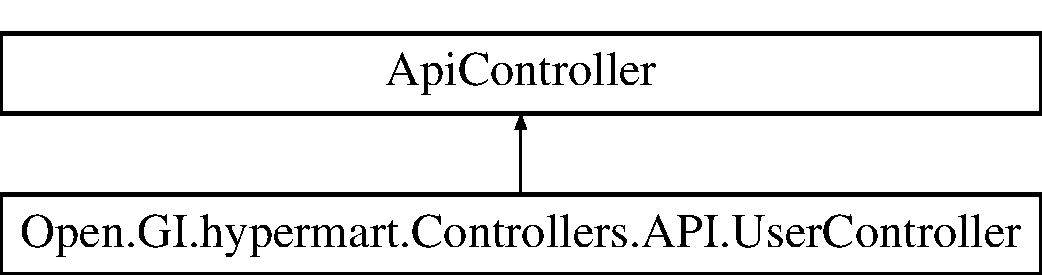
\includegraphics[height=2.000000cm]{class_open_1_1_g_i_1_1hypermart_1_1_controllers_1_1_a_p_i_1_1_user_controller}
\end{center}
\end{figure}
\subsection*{Public Member Functions}
\begin{DoxyCompactItemize}
\item 
\hyperlink{class_open_1_1_g_i_1_1hypermart_1_1_data_transformation_objects_1_1_user_d_t_o}{User\+D\+TO} \hyperlink{class_open_1_1_g_i_1_1hypermart_1_1_controllers_1_1_a_p_i_1_1_user_controller_af2896a942d750bcc948228c298221f15}{Details} (string userid)
\begin{DoxyCompactList}\small\item\em Retrieves the user information from the directory. \end{DoxyCompactList}\end{DoxyCompactItemize}


\subsection{Detailed Description}
This is the Open\+GI \hyperlink{namespace_open_1_1_g_i_1_1hypermart_1_1_controllers_1_1_a_p_i}{A\+PI} layer for interacting with users. This \hyperlink{namespace_open_1_1_g_i_1_1hypermart_1_1_controllers_1_1_a_p_i}{A\+PI} layer allows user details to be retireved from Active Directory. 

Required minimal configuration, but does require a directory services of sorts -\/ this should work with the Active Directory Lightweight Directory Services (to be confirmed). 

\subsection{Member Function Documentation}
\hypertarget{class_open_1_1_g_i_1_1hypermart_1_1_controllers_1_1_a_p_i_1_1_user_controller_af2896a942d750bcc948228c298221f15}{}\label{class_open_1_1_g_i_1_1hypermart_1_1_controllers_1_1_a_p_i_1_1_user_controller_af2896a942d750bcc948228c298221f15} 
\index{Open\+::\+G\+I\+::hypermart\+::\+Controllers\+::\+A\+P\+I\+::\+User\+Controller@{Open\+::\+G\+I\+::hypermart\+::\+Controllers\+::\+A\+P\+I\+::\+User\+Controller}!Details@{Details}}
\index{Details@{Details}!Open\+::\+G\+I\+::hypermart\+::\+Controllers\+::\+A\+P\+I\+::\+User\+Controller@{Open\+::\+G\+I\+::hypermart\+::\+Controllers\+::\+A\+P\+I\+::\+User\+Controller}}
\subsubsection{\texorpdfstring{Details()}{Details()}}
{\footnotesize\ttfamily \hyperlink{class_open_1_1_g_i_1_1hypermart_1_1_data_transformation_objects_1_1_user_d_t_o}{User\+D\+TO} Open.\+G\+I.\+hypermart.\+Controllers.\+A\+P\+I.\+User\+Controller.\+Details (\begin{DoxyParamCaption}\item[{string}]{userid }\end{DoxyParamCaption})}



Retrieves the user information from the directory. 


\begin{DoxyParams}{Parameters}
{\em userid} & \\
\hline
\end{DoxyParams}
\begin{DoxyReturn}{Returns}

\end{DoxyReturn}


The documentation for this class was generated from the following file\+:\begin{DoxyCompactItemize}
\item 
C\+:/\+Projects/\+App-\/\+Utility-\/\+Store/\+Open.\+G\+I.\+hypermart/\+Controllers/\+A\+P\+I/\hyperlink{_a_p_i_2_user_controller_8cs}{User\+Controller.\+cs}\end{DoxyCompactItemize}

\section{Open.\+G\+I.\+hypermart.\+Controllers.\+User\+Controller Class Reference}
\label{class_open_1_1_g_i_1_1hypermart_1_1_controllers_1_1_user_controller}\index{Open.\+G\+I.\+hypermart.\+Controllers.\+User\+Controller@{Open.\+G\+I.\+hypermart.\+Controllers.\+User\+Controller}}


User Controller  


Inheritance diagram for Open.\+G\+I.\+hypermart.\+Controllers.\+User\+Controller\+:\begin{figure}[H]
\begin{center}
\leavevmode
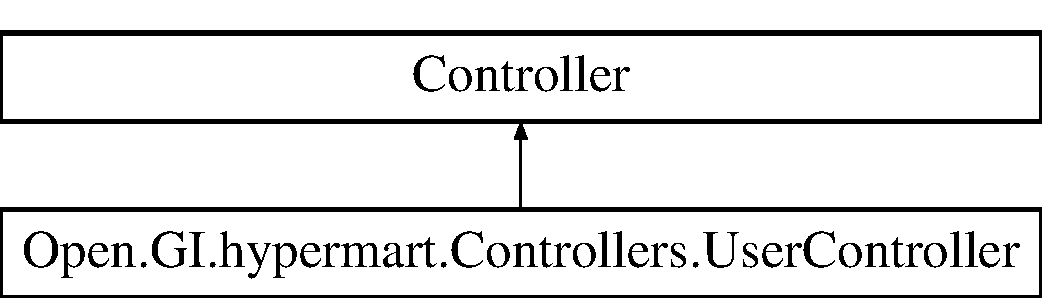
\includegraphics[height=2.000000cm]{class_open_1_1_g_i_1_1hypermart_1_1_controllers_1_1_user_controller}
\end{center}
\end{figure}
\subsection*{Public Member Functions}
\begin{DoxyCompactItemize}
\item 
Action\+Result \textbf{ Details} (string id)
\begin{DoxyCompactList}\small\item\em Detailses the specified userid. \end{DoxyCompactList}\item 
Action\+Result \textbf{ popup\+\_\+\+Details} (string userid)
\begin{DoxyCompactList}\small\item\em Detailses the specified userid. \end{DoxyCompactList}\end{DoxyCompactItemize}


\subsection{Detailed Description}
User Controller 

\begin{DoxySeeAlso}{See also}
System.\+Web.\+Mvc.\+Controller


\end{DoxySeeAlso}


Definition at line 13 of file User\+Controller.\+cs.



\subsection{Member Function Documentation}
\mbox{\label{class_open_1_1_g_i_1_1hypermart_1_1_controllers_1_1_user_controller_a4627a7a94b713760f00050bac936a54f}} 
\index{Open\+::\+G\+I\+::hypermart\+::\+Controllers\+::\+User\+Controller@{Open\+::\+G\+I\+::hypermart\+::\+Controllers\+::\+User\+Controller}!Details@{Details}}
\index{Details@{Details}!Open\+::\+G\+I\+::hypermart\+::\+Controllers\+::\+User\+Controller@{Open\+::\+G\+I\+::hypermart\+::\+Controllers\+::\+User\+Controller}}
\subsubsection{Details()}
{\footnotesize\ttfamily Action\+Result Open.\+G\+I.\+hypermart.\+Controllers.\+User\+Controller.\+Details (\begin{DoxyParamCaption}\item[{string}]{id }\end{DoxyParamCaption})}



Detailses the specified userid. 


\begin{DoxyParams}{Parameters}
{\em id} & The userid.\\
\hline
\end{DoxyParams}
\begin{DoxyReturn}{Returns}

\end{DoxyReturn}


Definition at line 28 of file User\+Controller.\+cs.

\mbox{\label{class_open_1_1_g_i_1_1hypermart_1_1_controllers_1_1_user_controller_a3168162b86edbdbd30a593fa6aca8e9f}} 
\index{Open\+::\+G\+I\+::hypermart\+::\+Controllers\+::\+User\+Controller@{Open\+::\+G\+I\+::hypermart\+::\+Controllers\+::\+User\+Controller}!popup\+\_\+\+Details@{popup\+\_\+\+Details}}
\index{popup\+\_\+\+Details@{popup\+\_\+\+Details}!Open\+::\+G\+I\+::hypermart\+::\+Controllers\+::\+User\+Controller@{Open\+::\+G\+I\+::hypermart\+::\+Controllers\+::\+User\+Controller}}
\subsubsection{popup\+\_\+\+Details()}
{\footnotesize\ttfamily Action\+Result Open.\+G\+I.\+hypermart.\+Controllers.\+User\+Controller.\+popup\+\_\+\+Details (\begin{DoxyParamCaption}\item[{string}]{userid }\end{DoxyParamCaption})}



Detailses the specified userid. 


\begin{DoxyParams}{Parameters}
{\em userid} & The userid.\\
\hline
\end{DoxyParams}
\begin{DoxyReturn}{Returns}

\end{DoxyReturn}


Definition at line 57 of file User\+Controller.\+cs.



The documentation for this class was generated from the following file\+:\begin{DoxyCompactItemize}
\item 
C\+:/\+Projects/\+App-\/\+Utility-\/\+Store/\+Open.\+G\+I.\+hypermart/\+Controllers/\textbf{ User\+Controller.\+cs}\end{DoxyCompactItemize}

\hypertarget{class_open_1_1_g_i_1_1hypermart_1_1_data_transformation_objects_1_1_user_d_t_o}{}\section{Open.\+G\+I.\+hypermart.\+Data\+Transformation\+Objects.\+User\+D\+T\+O Class Reference}
\label{class_open_1_1_g_i_1_1hypermart_1_1_data_transformation_objects_1_1_user_d_t_o}\index{Open.\+G\+I.\+hypermart.\+Data\+Transformation\+Objects.\+User\+D\+T\+O@{Open.\+G\+I.\+hypermart.\+Data\+Transformation\+Objects.\+User\+D\+T\+O}}


Class for Over-\/the-\/wire transmission of user information. If a user cannot be found, then an Unknown User will be returned.  


\subsection*{Public Member Functions}
\begin{DoxyCompactItemize}
\item 
\hyperlink{class_open_1_1_g_i_1_1hypermart_1_1_data_transformation_objects_1_1_user_d_t_o_ab715e6cac8b432f39c5fe6f22e3db645}{User\+D\+T\+O} ()
\begin{DoxyCompactList}\small\item\em Initializes a new instance of the \hyperlink{class_open_1_1_g_i_1_1hypermart_1_1_data_transformation_objects_1_1_user_d_t_o}{User\+D\+T\+O} class. \end{DoxyCompactList}\item 
\hyperlink{class_open_1_1_g_i_1_1hypermart_1_1_data_transformation_objects_1_1_user_d_t_o_a21ce2f8eaac0781bcc484f8eeca38404}{User\+D\+T\+O} (\hyperlink{class_open_1_1_g_i_1_1hypermart_1_1_models_1_1_user}{Open.\+G\+I.\+hypermart.\+Models.\+User} User\+To\+Wrap)
\begin{DoxyCompactList}\small\item\em Initializes a new instance of the \hyperlink{class_open_1_1_g_i_1_1hypermart_1_1_data_transformation_objects_1_1_user_d_t_o}{User\+D\+T\+O} class. \end{DoxyCompactList}\end{DoxyCompactItemize}
\subsection*{Properties}
\begin{DoxyCompactItemize}
\item 
string \hyperlink{class_open_1_1_g_i_1_1hypermart_1_1_data_transformation_objects_1_1_user_d_t_o_a123512619de906f987a3da0b7ec32bb1}{username}\hspace{0.3cm}{\ttfamily  \mbox{[}get, set\mbox{]}}
\begin{DoxyCompactList}\small\item\em Gets or sets the username. \end{DoxyCompactList}\item 
string \hyperlink{class_open_1_1_g_i_1_1hypermart_1_1_data_transformation_objects_1_1_user_d_t_o_a8ead06f70fbd3e0bcc72bf3aaae4fc9f}{Phone\+Numnber}\hspace{0.3cm}{\ttfamily  \mbox{[}get, set\mbox{]}}
\begin{DoxyCompactList}\small\item\em Gets or sets the phone numnber. \end{DoxyCompactList}\item 
Byte\mbox{[}$\,$\mbox{]} \hyperlink{class_open_1_1_g_i_1_1hypermart_1_1_data_transformation_objects_1_1_user_d_t_o_a3e4447b4cd2ef861c95c1e9162cbceb1}{Photo\+\_\+byte\+Array}\hspace{0.3cm}{\ttfamily  \mbox{[}get, set\mbox{]}}
\begin{DoxyCompactList}\small\item\em Base 64 encoded png image. \end{DoxyCompactList}\item 
string \hyperlink{class_open_1_1_g_i_1_1hypermart_1_1_data_transformation_objects_1_1_user_d_t_o_a96fdfcc9b2aa36fb35f6612b9e99b535}{Email}\hspace{0.3cm}{\ttfamily  \mbox{[}get, set\mbox{]}}
\begin{DoxyCompactList}\small\item\em Gets or sets the email. \end{DoxyCompactList}\item 
string \hyperlink{class_open_1_1_g_i_1_1hypermart_1_1_data_transformation_objects_1_1_user_d_t_o_a7a436dea35ee6683f2f7f0c3e9551d08}{Job\+Title}\hspace{0.3cm}{\ttfamily  \mbox{[}get, set\mbox{]}}
\begin{DoxyCompactList}\small\item\em Gets or sets the job title. \end{DoxyCompactList}\end{DoxyCompactItemize}


\subsection{Detailed Description}
Class for Over-\/the-\/wire transmission of user information. If a user cannot be found, then an Unknown User will be returned. 



Definition at line 14 of file User\+D\+T\+O.\+cs.



\subsection{Constructor \& Destructor Documentation}
\hypertarget{class_open_1_1_g_i_1_1hypermart_1_1_data_transformation_objects_1_1_user_d_t_o_ab715e6cac8b432f39c5fe6f22e3db645}{}\index{Open\+::\+G\+I\+::hypermart\+::\+Data\+Transformation\+Objects\+::\+User\+D\+T\+O@{Open\+::\+G\+I\+::hypermart\+::\+Data\+Transformation\+Objects\+::\+User\+D\+T\+O}!User\+D\+T\+O@{User\+D\+T\+O}}
\index{User\+D\+T\+O@{User\+D\+T\+O}!Open\+::\+G\+I\+::hypermart\+::\+Data\+Transformation\+Objects\+::\+User\+D\+T\+O@{Open\+::\+G\+I\+::hypermart\+::\+Data\+Transformation\+Objects\+::\+User\+D\+T\+O}}
\subsubsection[{User\+D\+T\+O()}]{\setlength{\rightskip}{0pt plus 5cm}Open.\+G\+I.\+hypermart.\+Data\+Transformation\+Objects.\+User\+D\+T\+O.\+User\+D\+T\+O (
\begin{DoxyParamCaption}
{}
\end{DoxyParamCaption}
)}\label{class_open_1_1_g_i_1_1hypermart_1_1_data_transformation_objects_1_1_user_d_t_o_ab715e6cac8b432f39c5fe6f22e3db645}


Initializes a new instance of the \hyperlink{class_open_1_1_g_i_1_1hypermart_1_1_data_transformation_objects_1_1_user_d_t_o}{User\+D\+T\+O} class. 



Definition at line 19 of file User\+D\+T\+O.\+cs.

\hypertarget{class_open_1_1_g_i_1_1hypermart_1_1_data_transformation_objects_1_1_user_d_t_o_a21ce2f8eaac0781bcc484f8eeca38404}{}\index{Open\+::\+G\+I\+::hypermart\+::\+Data\+Transformation\+Objects\+::\+User\+D\+T\+O@{Open\+::\+G\+I\+::hypermart\+::\+Data\+Transformation\+Objects\+::\+User\+D\+T\+O}!User\+D\+T\+O@{User\+D\+T\+O}}
\index{User\+D\+T\+O@{User\+D\+T\+O}!Open\+::\+G\+I\+::hypermart\+::\+Data\+Transformation\+Objects\+::\+User\+D\+T\+O@{Open\+::\+G\+I\+::hypermart\+::\+Data\+Transformation\+Objects\+::\+User\+D\+T\+O}}
\subsubsection[{User\+D\+T\+O(\+Open.\+G\+I.\+hypermart.\+Models.\+User User\+To\+Wrap)}]{\setlength{\rightskip}{0pt plus 5cm}Open.\+G\+I.\+hypermart.\+Data\+Transformation\+Objects.\+User\+D\+T\+O.\+User\+D\+T\+O (
\begin{DoxyParamCaption}
\item[{{\bf Open.\+G\+I.\+hypermart.\+Models.\+User}}]{User\+To\+Wrap}
\end{DoxyParamCaption}
)}\label{class_open_1_1_g_i_1_1hypermart_1_1_data_transformation_objects_1_1_user_d_t_o_a21ce2f8eaac0781bcc484f8eeca38404}


Initializes a new instance of the \hyperlink{class_open_1_1_g_i_1_1hypermart_1_1_data_transformation_objects_1_1_user_d_t_o}{User\+D\+T\+O} class. 


\begin{DoxyParams}{Parameters}
{\em User\+To\+Wrap} & The user to wrap.\\
\hline
\end{DoxyParams}


Definition at line 28 of file User\+D\+T\+O.\+cs.



\subsection{Property Documentation}
\hypertarget{class_open_1_1_g_i_1_1hypermart_1_1_data_transformation_objects_1_1_user_d_t_o_a96fdfcc9b2aa36fb35f6612b9e99b535}{}\index{Open\+::\+G\+I\+::hypermart\+::\+Data\+Transformation\+Objects\+::\+User\+D\+T\+O@{Open\+::\+G\+I\+::hypermart\+::\+Data\+Transformation\+Objects\+::\+User\+D\+T\+O}!Email@{Email}}
\index{Email@{Email}!Open\+::\+G\+I\+::hypermart\+::\+Data\+Transformation\+Objects\+::\+User\+D\+T\+O@{Open\+::\+G\+I\+::hypermart\+::\+Data\+Transformation\+Objects\+::\+User\+D\+T\+O}}
\subsubsection[{Email}]{\setlength{\rightskip}{0pt plus 5cm}string Open.\+G\+I.\+hypermart.\+Data\+Transformation\+Objects.\+User\+D\+T\+O.\+Email\hspace{0.3cm}{\ttfamily [get]}, {\ttfamily [set]}}\label{class_open_1_1_g_i_1_1hypermart_1_1_data_transformation_objects_1_1_user_d_t_o_a96fdfcc9b2aa36fb35f6612b9e99b535}


Gets or sets the email. 

The email. 

Definition at line 60 of file User\+D\+T\+O.\+cs.

\hypertarget{class_open_1_1_g_i_1_1hypermart_1_1_data_transformation_objects_1_1_user_d_t_o_a7a436dea35ee6683f2f7f0c3e9551d08}{}\index{Open\+::\+G\+I\+::hypermart\+::\+Data\+Transformation\+Objects\+::\+User\+D\+T\+O@{Open\+::\+G\+I\+::hypermart\+::\+Data\+Transformation\+Objects\+::\+User\+D\+T\+O}!Job\+Title@{Job\+Title}}
\index{Job\+Title@{Job\+Title}!Open\+::\+G\+I\+::hypermart\+::\+Data\+Transformation\+Objects\+::\+User\+D\+T\+O@{Open\+::\+G\+I\+::hypermart\+::\+Data\+Transformation\+Objects\+::\+User\+D\+T\+O}}
\subsubsection[{Job\+Title}]{\setlength{\rightskip}{0pt plus 5cm}string Open.\+G\+I.\+hypermart.\+Data\+Transformation\+Objects.\+User\+D\+T\+O.\+Job\+Title\hspace{0.3cm}{\ttfamily [get]}, {\ttfamily [set]}}\label{class_open_1_1_g_i_1_1hypermart_1_1_data_transformation_objects_1_1_user_d_t_o_a7a436dea35ee6683f2f7f0c3e9551d08}


Gets or sets the job title. 

The job title. 

Definition at line 67 of file User\+D\+T\+O.\+cs.

\hypertarget{class_open_1_1_g_i_1_1hypermart_1_1_data_transformation_objects_1_1_user_d_t_o_a8ead06f70fbd3e0bcc72bf3aaae4fc9f}{}\index{Open\+::\+G\+I\+::hypermart\+::\+Data\+Transformation\+Objects\+::\+User\+D\+T\+O@{Open\+::\+G\+I\+::hypermart\+::\+Data\+Transformation\+Objects\+::\+User\+D\+T\+O}!Phone\+Numnber@{Phone\+Numnber}}
\index{Phone\+Numnber@{Phone\+Numnber}!Open\+::\+G\+I\+::hypermart\+::\+Data\+Transformation\+Objects\+::\+User\+D\+T\+O@{Open\+::\+G\+I\+::hypermart\+::\+Data\+Transformation\+Objects\+::\+User\+D\+T\+O}}
\subsubsection[{Phone\+Numnber}]{\setlength{\rightskip}{0pt plus 5cm}string Open.\+G\+I.\+hypermart.\+Data\+Transformation\+Objects.\+User\+D\+T\+O.\+Phone\+Numnber\hspace{0.3cm}{\ttfamily [get]}, {\ttfamily [set]}}\label{class_open_1_1_g_i_1_1hypermart_1_1_data_transformation_objects_1_1_user_d_t_o_a8ead06f70fbd3e0bcc72bf3aaae4fc9f}


Gets or sets the phone numnber. 

The phone numnber. 

Definition at line 49 of file User\+D\+T\+O.\+cs.

\hypertarget{class_open_1_1_g_i_1_1hypermart_1_1_data_transformation_objects_1_1_user_d_t_o_a3e4447b4cd2ef861c95c1e9162cbceb1}{}\index{Open\+::\+G\+I\+::hypermart\+::\+Data\+Transformation\+Objects\+::\+User\+D\+T\+O@{Open\+::\+G\+I\+::hypermart\+::\+Data\+Transformation\+Objects\+::\+User\+D\+T\+O}!Photo\+\_\+byte\+Array@{Photo\+\_\+byte\+Array}}
\index{Photo\+\_\+byte\+Array@{Photo\+\_\+byte\+Array}!Open\+::\+G\+I\+::hypermart\+::\+Data\+Transformation\+Objects\+::\+User\+D\+T\+O@{Open\+::\+G\+I\+::hypermart\+::\+Data\+Transformation\+Objects\+::\+User\+D\+T\+O}}
\subsubsection[{Photo\+\_\+byte\+Array}]{\setlength{\rightskip}{0pt plus 5cm}Byte \mbox{[}$\,$\mbox{]} Open.\+G\+I.\+hypermart.\+Data\+Transformation\+Objects.\+User\+D\+T\+O.\+Photo\+\_\+byte\+Array\hspace{0.3cm}{\ttfamily [get]}, {\ttfamily [set]}}\label{class_open_1_1_g_i_1_1hypermart_1_1_data_transformation_objects_1_1_user_d_t_o_a3e4447b4cd2ef861c95c1e9162cbceb1}


Base 64 encoded png image. 



Definition at line 53 of file User\+D\+T\+O.\+cs.

\hypertarget{class_open_1_1_g_i_1_1hypermart_1_1_data_transformation_objects_1_1_user_d_t_o_a123512619de906f987a3da0b7ec32bb1}{}\index{Open\+::\+G\+I\+::hypermart\+::\+Data\+Transformation\+Objects\+::\+User\+D\+T\+O@{Open\+::\+G\+I\+::hypermart\+::\+Data\+Transformation\+Objects\+::\+User\+D\+T\+O}!username@{username}}
\index{username@{username}!Open\+::\+G\+I\+::hypermart\+::\+Data\+Transformation\+Objects\+::\+User\+D\+T\+O@{Open\+::\+G\+I\+::hypermart\+::\+Data\+Transformation\+Objects\+::\+User\+D\+T\+O}}
\subsubsection[{username}]{\setlength{\rightskip}{0pt plus 5cm}string Open.\+G\+I.\+hypermart.\+Data\+Transformation\+Objects.\+User\+D\+T\+O.\+username\hspace{0.3cm}{\ttfamily [get]}, {\ttfamily [set]}}\label{class_open_1_1_g_i_1_1hypermart_1_1_data_transformation_objects_1_1_user_d_t_o_a123512619de906f987a3da0b7ec32bb1}


Gets or sets the username. 

The username. 

Definition at line 42 of file User\+D\+T\+O.\+cs.



The documentation for this class was generated from the following file\+:\begin{DoxyCompactItemize}
\item 
C\+:/\+Projects/\+App-\/\+Utility-\/\+Store/\+Open.\+G\+I.\+hypermart/\+Data\+Transformation\+Objects/\hyperlink{_user_d_t_o_8cs}{User\+D\+T\+O.\+cs}\end{DoxyCompactItemize}

\section{Open.\+G\+I.\+hypermart.\+Models.\+User\+Model Class Reference}
\label{class_open_1_1_g_i_1_1hypermart_1_1_models_1_1_user_model}\index{Open.\+G\+I.\+hypermart.\+Models.\+User\+Model@{Open.\+G\+I.\+hypermart.\+Models.\+User\+Model}}


 


\subsection*{Properties}
\begin{DoxyCompactItemize}
\item 
string \textbf{ User\+Name}\hspace{0.3cm}{\ttfamily  [get, set]}
\begin{DoxyCompactList}\small\item\em Gets or sets the name of the user. \end{DoxyCompactList}\item 
string \textbf{ Password}\hspace{0.3cm}{\ttfamily  [get, set]}
\begin{DoxyCompactList}\small\item\em Gets or sets the password. \end{DoxyCompactList}\item 
string \textbf{ Confirm\+Password}\hspace{0.3cm}{\ttfamily  [get, set]}
\begin{DoxyCompactList}\small\item\em Gets or sets the confirm password. \end{DoxyCompactList}\end{DoxyCompactItemize}


\subsection{Detailed Description}




Definition at line 13 of file User\+Model.\+cs.



\subsection{Property Documentation}
\mbox{\label{class_open_1_1_g_i_1_1hypermart_1_1_models_1_1_user_model_a671662415ad880aaf5c2e7b43a83faa9}} 
\index{Open\+::\+G\+I\+::hypermart\+::\+Models\+::\+User\+Model@{Open\+::\+G\+I\+::hypermart\+::\+Models\+::\+User\+Model}!Confirm\+Password@{Confirm\+Password}}
\index{Confirm\+Password@{Confirm\+Password}!Open\+::\+G\+I\+::hypermart\+::\+Models\+::\+User\+Model@{Open\+::\+G\+I\+::hypermart\+::\+Models\+::\+User\+Model}}
\subsubsection{Confirm\+Password}
{\footnotesize\ttfamily string Open.\+G\+I.\+hypermart.\+Models.\+User\+Model.\+Confirm\+Password\hspace{0.3cm}{\ttfamily [get]}, {\ttfamily [set]}}



Gets or sets the confirm password. 

The confirm password. 

Definition at line 44 of file User\+Model.\+cs.

\mbox{\label{class_open_1_1_g_i_1_1hypermart_1_1_models_1_1_user_model_a7444f518307d0a5ee95b237243a26247}} 
\index{Open\+::\+G\+I\+::hypermart\+::\+Models\+::\+User\+Model@{Open\+::\+G\+I\+::hypermart\+::\+Models\+::\+User\+Model}!Password@{Password}}
\index{Password@{Password}!Open\+::\+G\+I\+::hypermart\+::\+Models\+::\+User\+Model@{Open\+::\+G\+I\+::hypermart\+::\+Models\+::\+User\+Model}}
\subsubsection{Password}
{\footnotesize\ttfamily string Open.\+G\+I.\+hypermart.\+Models.\+User\+Model.\+Password\hspace{0.3cm}{\ttfamily [get]}, {\ttfamily [set]}}



Gets or sets the password. 

The password. 

Definition at line 34 of file User\+Model.\+cs.

\mbox{\label{class_open_1_1_g_i_1_1hypermart_1_1_models_1_1_user_model_aa873e73ce7a4470c31e78f7cc86c25ad}} 
\index{Open\+::\+G\+I\+::hypermart\+::\+Models\+::\+User\+Model@{Open\+::\+G\+I\+::hypermart\+::\+Models\+::\+User\+Model}!User\+Name@{User\+Name}}
\index{User\+Name@{User\+Name}!Open\+::\+G\+I\+::hypermart\+::\+Models\+::\+User\+Model@{Open\+::\+G\+I\+::hypermart\+::\+Models\+::\+User\+Model}}
\subsubsection{User\+Name}
{\footnotesize\ttfamily string Open.\+G\+I.\+hypermart.\+Models.\+User\+Model.\+User\+Name\hspace{0.3cm}{\ttfamily [get]}, {\ttfamily [set]}}



Gets or sets the name of the user. 

The name of the user. 

Definition at line 23 of file User\+Model.\+cs.



The documentation for this class was generated from the following file\+:\begin{DoxyCompactItemize}
\item 
C\+:/\+Projects/\+App-\/\+Utility-\/\+Store/\+Open.\+G\+I.\+hypermart/\+Models/\textbf{ User\+Model.\+cs}\end{DoxyCompactItemize}

\section{Open.\+G\+I.\+hypermart.\+Controllers.\+A\+P\+I.\+Values\+Controller Class Reference}
\label{class_open_1_1_g_i_1_1hypermart_1_1_controllers_1_1_a_p_i_1_1_values_controller}\index{Open.\+G\+I.\+hypermart.\+Controllers.\+A\+P\+I.\+Values\+Controller@{Open.\+G\+I.\+hypermart.\+Controllers.\+A\+P\+I.\+Values\+Controller}}


 


Inheritance diagram for Open.\+G\+I.\+hypermart.\+Controllers.\+A\+P\+I.\+Values\+Controller\+:\begin{figure}[H]
\begin{center}
\leavevmode
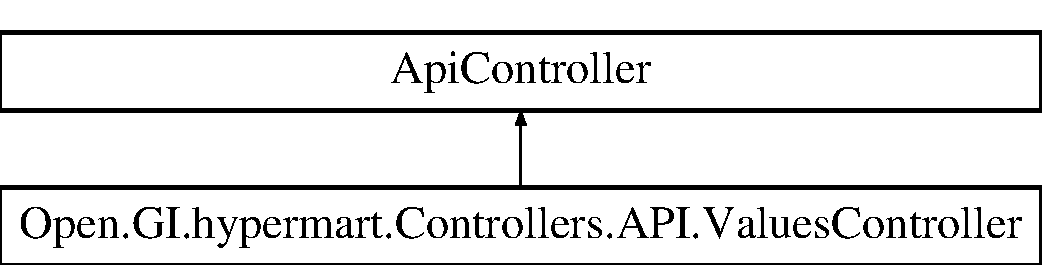
\includegraphics[height=2.000000cm]{class_open_1_1_g_i_1_1hypermart_1_1_controllers_1_1_a_p_i_1_1_values_controller}
\end{center}
\end{figure}
\subsection*{Public Member Functions}
\begin{DoxyCompactItemize}
\item 
I\+Enumerable$<$ string $>$ \textbf{ Get\+By\+Status} (int \textbf{ Status})
\begin{DoxyCompactList}\small\item\em Gets all of the values \end{DoxyCompactList}\item 
I\+Enumerable$<$ string $>$ \textbf{ Get} ()
\begin{DoxyCompactList}\small\item\em Gets all of the values \end{DoxyCompactList}\item 
string \textbf{ Get} (int id)
\begin{DoxyCompactList}\small\item\em Gets the specified identifier. \end{DoxyCompactList}\item 
void \textbf{ Post} ([From\+Body]string value)
\begin{DoxyCompactList}\small\item\em Posts the specified value. \end{DoxyCompactList}\item 
void \textbf{ Put} (int id, [From\+Body]string value)
\begin{DoxyCompactList}\small\item\em Puts the specified identifier. \end{DoxyCompactList}\item 
void \textbf{ Delete} (int id)
\begin{DoxyCompactList}\small\item\em Deletes the specified identifier. \end{DoxyCompactList}\end{DoxyCompactItemize}


\subsection{Detailed Description}


Values Controller 

\begin{DoxySeeAlso}{See also}
System.\+Web.\+Http.\+Api\+Controller


\end{DoxySeeAlso}


Definition at line 16 of file Values\+Controller.\+cs.



\subsection{Member Function Documentation}
\mbox{\label{class_open_1_1_g_i_1_1hypermart_1_1_controllers_1_1_a_p_i_1_1_values_controller_aac5ef946899bcf7c07bdf860004f8c1a}} 
\index{Open\+::\+G\+I\+::hypermart\+::\+Controllers\+::\+A\+P\+I\+::\+Values\+Controller@{Open\+::\+G\+I\+::hypermart\+::\+Controllers\+::\+A\+P\+I\+::\+Values\+Controller}!Delete@{Delete}}
\index{Delete@{Delete}!Open\+::\+G\+I\+::hypermart\+::\+Controllers\+::\+A\+P\+I\+::\+Values\+Controller@{Open\+::\+G\+I\+::hypermart\+::\+Controllers\+::\+A\+P\+I\+::\+Values\+Controller}}
\subsubsection{Delete()}
{\footnotesize\ttfamily void Open.\+G\+I.\+hypermart.\+Controllers.\+A\+P\+I.\+Values\+Controller.\+Delete (\begin{DoxyParamCaption}\item[{int}]{id }\end{DoxyParamCaption})}



Deletes the specified identifier. 


\begin{DoxyParams}{Parameters}
{\em id} & The identifier.\\
\hline
\end{DoxyParams}


Definition at line 70 of file Values\+Controller.\+cs.

\mbox{\label{class_open_1_1_g_i_1_1hypermart_1_1_controllers_1_1_a_p_i_1_1_values_controller_a22701a876d9570628f81c46396db9470}} 
\index{Open\+::\+G\+I\+::hypermart\+::\+Controllers\+::\+A\+P\+I\+::\+Values\+Controller@{Open\+::\+G\+I\+::hypermart\+::\+Controllers\+::\+A\+P\+I\+::\+Values\+Controller}!Get@{Get}}
\index{Get@{Get}!Open\+::\+G\+I\+::hypermart\+::\+Controllers\+::\+A\+P\+I\+::\+Values\+Controller@{Open\+::\+G\+I\+::hypermart\+::\+Controllers\+::\+A\+P\+I\+::\+Values\+Controller}}
\subsubsection{Get()\hspace{0.1cm}{\footnotesize\ttfamily [1/2]}}
{\footnotesize\ttfamily I\+Enumerable$<$string$>$ Open.\+G\+I.\+hypermart.\+Controllers.\+A\+P\+I.\+Values\+Controller.\+Get (\begin{DoxyParamCaption}{ }\end{DoxyParamCaption})}



Gets all of the values 

\begin{DoxyReturn}{Returns}

\end{DoxyReturn}


Definition at line 34 of file Values\+Controller.\+cs.

\mbox{\label{class_open_1_1_g_i_1_1hypermart_1_1_controllers_1_1_a_p_i_1_1_values_controller_a939097635499ed1d2f82186a1d85d2d4}} 
\index{Open\+::\+G\+I\+::hypermart\+::\+Controllers\+::\+A\+P\+I\+::\+Values\+Controller@{Open\+::\+G\+I\+::hypermart\+::\+Controllers\+::\+A\+P\+I\+::\+Values\+Controller}!Get@{Get}}
\index{Get@{Get}!Open\+::\+G\+I\+::hypermart\+::\+Controllers\+::\+A\+P\+I\+::\+Values\+Controller@{Open\+::\+G\+I\+::hypermart\+::\+Controllers\+::\+A\+P\+I\+::\+Values\+Controller}}
\subsubsection{Get()\hspace{0.1cm}{\footnotesize\ttfamily [2/2]}}
{\footnotesize\ttfamily string Open.\+G\+I.\+hypermart.\+Controllers.\+A\+P\+I.\+Values\+Controller.\+Get (\begin{DoxyParamCaption}\item[{int}]{id }\end{DoxyParamCaption})}



Gets the specified identifier. 


\begin{DoxyParams}{Parameters}
{\em id} & The identifier.\\
\hline
\end{DoxyParams}
\begin{DoxyReturn}{Returns}

\end{DoxyReturn}


Definition at line 44 of file Values\+Controller.\+cs.

\mbox{\label{class_open_1_1_g_i_1_1hypermart_1_1_controllers_1_1_a_p_i_1_1_values_controller_a0f58764e60950048b68217098361ea62}} 
\index{Open\+::\+G\+I\+::hypermart\+::\+Controllers\+::\+A\+P\+I\+::\+Values\+Controller@{Open\+::\+G\+I\+::hypermart\+::\+Controllers\+::\+A\+P\+I\+::\+Values\+Controller}!Get\+By\+Status@{Get\+By\+Status}}
\index{Get\+By\+Status@{Get\+By\+Status}!Open\+::\+G\+I\+::hypermart\+::\+Controllers\+::\+A\+P\+I\+::\+Values\+Controller@{Open\+::\+G\+I\+::hypermart\+::\+Controllers\+::\+A\+P\+I\+::\+Values\+Controller}}
\subsubsection{Get\+By\+Status()}
{\footnotesize\ttfamily I\+Enumerable$<$string$>$ Open.\+G\+I.\+hypermart.\+Controllers.\+A\+P\+I.\+Values\+Controller.\+Get\+By\+Status (\begin{DoxyParamCaption}\item[{int}]{Status }\end{DoxyParamCaption})}



Gets all of the values 

\begin{DoxyReturn}{Returns}

\end{DoxyReturn}


Definition at line 23 of file Values\+Controller.\+cs.

\mbox{\label{class_open_1_1_g_i_1_1hypermart_1_1_controllers_1_1_a_p_i_1_1_values_controller_a4b0c28944cf2577d0883f17466b45453}} 
\index{Open\+::\+G\+I\+::hypermart\+::\+Controllers\+::\+A\+P\+I\+::\+Values\+Controller@{Open\+::\+G\+I\+::hypermart\+::\+Controllers\+::\+A\+P\+I\+::\+Values\+Controller}!Post@{Post}}
\index{Post@{Post}!Open\+::\+G\+I\+::hypermart\+::\+Controllers\+::\+A\+P\+I\+::\+Values\+Controller@{Open\+::\+G\+I\+::hypermart\+::\+Controllers\+::\+A\+P\+I\+::\+Values\+Controller}}
\subsubsection{Post()}
{\footnotesize\ttfamily void Open.\+G\+I.\+hypermart.\+Controllers.\+A\+P\+I.\+Values\+Controller.\+Post (\begin{DoxyParamCaption}\item[{[\+From\+Body] string}]{value }\end{DoxyParamCaption})}



Posts the specified value. 


\begin{DoxyParams}{Parameters}
{\em value} & The value.\\
\hline
\end{DoxyParams}


Definition at line 53 of file Values\+Controller.\+cs.

\mbox{\label{class_open_1_1_g_i_1_1hypermart_1_1_controllers_1_1_a_p_i_1_1_values_controller_a1639499e0a18f82e61335c94c344ad31}} 
\index{Open\+::\+G\+I\+::hypermart\+::\+Controllers\+::\+A\+P\+I\+::\+Values\+Controller@{Open\+::\+G\+I\+::hypermart\+::\+Controllers\+::\+A\+P\+I\+::\+Values\+Controller}!Put@{Put}}
\index{Put@{Put}!Open\+::\+G\+I\+::hypermart\+::\+Controllers\+::\+A\+P\+I\+::\+Values\+Controller@{Open\+::\+G\+I\+::hypermart\+::\+Controllers\+::\+A\+P\+I\+::\+Values\+Controller}}
\subsubsection{Put()}
{\footnotesize\ttfamily void Open.\+G\+I.\+hypermart.\+Controllers.\+A\+P\+I.\+Values\+Controller.\+Put (\begin{DoxyParamCaption}\item[{int}]{id,  }\item[{[\+From\+Body] string}]{value }\end{DoxyParamCaption})}



Puts the specified identifier. 


\begin{DoxyParams}{Parameters}
{\em id} & The identifier.\\
\hline
{\em value} & The value.\\
\hline
\end{DoxyParams}


Definition at line 62 of file Values\+Controller.\+cs.



The documentation for this class was generated from the following file\+:\begin{DoxyCompactItemize}
\item 
C\+:/\+Projects/\+App-\/\+Utility-\/\+Store/\+Open.\+G\+I.\+hypermart/\+Controllers/\+A\+P\+I/\textbf{ Values\+Controller.\+cs}\end{DoxyCompactItemize}

\hypertarget{class_open_1_1_g_i_1_1hypermart_1_1_helpers_1_1_view_renderer}{}\section{Open.\+G\+I.\+hypermart.\+Helpers.\+View\+Renderer Class Reference}
\label{class_open_1_1_g_i_1_1hypermart_1_1_helpers_1_1_view_renderer}\index{Open.\+G\+I.\+hypermart.\+Helpers.\+View\+Renderer@{Open.\+G\+I.\+hypermart.\+Helpers.\+View\+Renderer}}


Class that renders M\+VC views to a string using the standard M\+VC View Engine to render the view.  


\subsection*{Public Member Functions}
\begin{DoxyCompactItemize}
\item 
\hyperlink{class_open_1_1_g_i_1_1hypermart_1_1_helpers_1_1_view_renderer_aabe19f0b091fc4a5a2dbef6c898eaef4}{View\+Renderer} (Controller\+Context controller\+Context=null)
\begin{DoxyCompactList}\small\item\em Initializes the \hyperlink{class_open_1_1_g_i_1_1hypermart_1_1_helpers_1_1_view_renderer}{View\+Renderer} with a Context. \end{DoxyCompactList}\item 
string \hyperlink{class_open_1_1_g_i_1_1hypermart_1_1_helpers_1_1_view_renderer_af8383dd6d43af50ba6433ea8fa9c03f2}{Render\+View\+To\+String} (string view\+Path, object model=null)
\begin{DoxyCompactList}\small\item\em Renders a full M\+VC view to a string. Will render with the full M\+VC View engine including running \+\_\+\+View\+Start and merging into \+\_\+\+Layout \end{DoxyCompactList}\item 
void \hyperlink{class_open_1_1_g_i_1_1hypermart_1_1_helpers_1_1_view_renderer_af04c462b2dc2f610f0442f8d5718055a}{Render\+View} (string view\+Path, object model, Text\+Writer writer)
\begin{DoxyCompactList}\small\item\em Renders a full M\+VC view to a writer. Will render with the full M\+VC View engine including running \+\_\+\+View\+Start and merging into \+\_\+\+Layout \end{DoxyCompactList}\item 
string \hyperlink{class_open_1_1_g_i_1_1hypermart_1_1_helpers_1_1_view_renderer_a2afbe1ea2ffd68f08dcd28309fd42744}{Render\+Partial\+View\+To\+String} (string view\+Path, object model=null)
\begin{DoxyCompactList}\small\item\em Renders a partial M\+VC view to string. Use this method to render a partial view that doesn\textquotesingle{}t merge with \+\_\+\+Layout and doesn\textquotesingle{}t fire \+\_\+\+View\+Start. \end{DoxyCompactList}\item 
void \hyperlink{class_open_1_1_g_i_1_1hypermart_1_1_helpers_1_1_view_renderer_af41730f2378765d4eacaae51b661ed45}{Render\+Partial\+View} (string view\+Path, object model, Text\+Writer writer)
\begin{DoxyCompactList}\small\item\em Renders a partial M\+VC view to given Writer. Use this method to render a partial view that doesn\textquotesingle{}t merge with \+\_\+\+Layout and doesn\textquotesingle{}t fire \+\_\+\+View\+Start. \end{DoxyCompactList}\end{DoxyCompactItemize}
\subsection*{Static Public Member Functions}
\begin{DoxyCompactItemize}
\item 
static string \hyperlink{class_open_1_1_g_i_1_1hypermart_1_1_helpers_1_1_view_renderer_a855fe4d3baa41ec21747aae42ab62c41}{Render\+View} (string view\+Path, object model=null, Controller\+Context controller\+Context=null)
\begin{DoxyCompactList}\small\item\em Renders a partial M\+VC view to string. Use this method to render a partial view that doesn\textquotesingle{}t merge with \+\_\+\+Layout and doesn\textquotesingle{}t fire \+\_\+\+View\+Start. \end{DoxyCompactList}\item 
static void \hyperlink{class_open_1_1_g_i_1_1hypermart_1_1_helpers_1_1_view_renderer_aad27a3171dfcb9a9d06351e637e249bf}{Render\+View} (string view\+Path, Text\+Writer writer, object model, Controller\+Context controller\+Context)
\begin{DoxyCompactList}\small\item\em Renders a partial M\+VC view to the given writer. Use this method to render a partial view that doesn\textquotesingle{}t merge with \+\_\+\+Layout and doesn\textquotesingle{}t fire \+\_\+\+View\+Start. \end{DoxyCompactList}\item 
static string \hyperlink{class_open_1_1_g_i_1_1hypermart_1_1_helpers_1_1_view_renderer_aba0a7e3bb189a5f1ce9ca4f8ace9c942}{Render\+View} (string view\+Path, object model, Controller\+Context controller\+Context, out string error\+Message)
\begin{DoxyCompactList}\small\item\em Renders a partial M\+VC view to string. Use this method to render a partial view that doesn\textquotesingle{}t merge with \+\_\+\+Layout and doesn\textquotesingle{}t fire \+\_\+\+View\+Start. \end{DoxyCompactList}\item 
static void \hyperlink{class_open_1_1_g_i_1_1hypermart_1_1_helpers_1_1_view_renderer_a54c412e138b0d84aba52d60003fe8f9f}{Render\+View} (string view\+Path, object model, Text\+Writer writer, Controller\+Context controller\+Context, out string error\+Message)
\begin{DoxyCompactList}\small\item\em Renders a partial M\+VC view to the given writer. Use this method to render a partial view that doesn\textquotesingle{}t merge with \+\_\+\+Layout and doesn\textquotesingle{}t fire \+\_\+\+View\+Start. \end{DoxyCompactList}\item 
static string \hyperlink{class_open_1_1_g_i_1_1hypermart_1_1_helpers_1_1_view_renderer_a57700e4f845a9f94635e35f3c495317e}{Render\+Partial\+View} (string view\+Path, object model=null, Controller\+Context controller\+Context=null)
\begin{DoxyCompactList}\small\item\em Renders a partial M\+VC view to string. Use this method to render a partial view that doesn\textquotesingle{}t merge with \+\_\+\+Layout and doesn\textquotesingle{}t fire \+\_\+\+View\+Start. \end{DoxyCompactList}\item 
static void \hyperlink{class_open_1_1_g_i_1_1hypermart_1_1_helpers_1_1_view_renderer_a4be45c477d06f4c6505f7d8c65bc988a}{Render\+Partial\+View} (string view\+Path, Text\+Writer writer, object model=null, Controller\+Context controller\+Context=null)
\begin{DoxyCompactList}\small\item\em Renders a partial M\+VC view to string. Use this method to render a partial view that doesn\textquotesingle{}t merge with \+\_\+\+Layout and doesn\textquotesingle{}t fire \+\_\+\+View\+Start. \end{DoxyCompactList}\item 
static T \hyperlink{class_open_1_1_g_i_1_1hypermart_1_1_helpers_1_1_view_renderer_a886a3c16dcc5798c5c820b87810e8c0f}{Create\+Controller$<$ T $>$} (Route\+Data route\+Data=null, params object\mbox{[}$\,$\mbox{]} parameters)
\begin{DoxyCompactList}\small\item\em Creates an instance of an M\+VC controller from scratch when no existing Controller\+Context is present \end{DoxyCompactList}\end{DoxyCompactItemize}
\subsection*{Protected Member Functions}
\begin{DoxyCompactItemize}
\item 
void \hyperlink{class_open_1_1_g_i_1_1hypermart_1_1_helpers_1_1_view_renderer_a2dda3a83d880019292d23e2cef0c8ac9}{Render\+View\+To\+Writer\+Internal} (string view\+Path, Text\+Writer writer, object model=null, bool partial=false)
\begin{DoxyCompactList}\small\item\em Internal method that handles rendering of either partial or or full views. \end{DoxyCompactList}\end{DoxyCompactItemize}
\subsection*{Properties}
\begin{DoxyCompactItemize}
\item 
Controller\+Context \hyperlink{class_open_1_1_g_i_1_1hypermart_1_1_helpers_1_1_view_renderer_ab42d020bf6988c82880809461bfd303b}{Context}\hspace{0.3cm}{\ttfamily  \mbox{[}get, set\mbox{]}}
\begin{DoxyCompactList}\small\item\em Required Controller Context \end{DoxyCompactList}\end{DoxyCompactItemize}


\subsection{Detailed Description}
Class that renders M\+VC views to a string using the standard M\+VC View Engine to render the view. 

Requires that A\+S\+P.\+N\+ET Http\+Context is present to work, but works outside of the context of M\+VC 

\subsection{Constructor \& Destructor Documentation}
\hypertarget{class_open_1_1_g_i_1_1hypermart_1_1_helpers_1_1_view_renderer_aabe19f0b091fc4a5a2dbef6c898eaef4}{}\label{class_open_1_1_g_i_1_1hypermart_1_1_helpers_1_1_view_renderer_aabe19f0b091fc4a5a2dbef6c898eaef4} 
\index{Open\+::\+G\+I\+::hypermart\+::\+Helpers\+::\+View\+Renderer@{Open\+::\+G\+I\+::hypermart\+::\+Helpers\+::\+View\+Renderer}!View\+Renderer@{View\+Renderer}}
\index{View\+Renderer@{View\+Renderer}!Open\+::\+G\+I\+::hypermart\+::\+Helpers\+::\+View\+Renderer@{Open\+::\+G\+I\+::hypermart\+::\+Helpers\+::\+View\+Renderer}}
\subsubsection{\texorpdfstring{View\+Renderer()}{ViewRenderer()}}
{\footnotesize\ttfamily Open.\+G\+I.\+hypermart.\+Helpers.\+View\+Renderer.\+View\+Renderer (\begin{DoxyParamCaption}\item[{Controller\+Context}]{controller\+Context = {\ttfamily null} }\end{DoxyParamCaption})}



Initializes the \hyperlink{class_open_1_1_g_i_1_1hypermart_1_1_helpers_1_1_view_renderer}{View\+Renderer} with a Context. 


\begin{DoxyParams}{Parameters}
{\em controller\+Context} & If you are running within the context of an A\+S\+P.\+N\+ET M\+VC request pass in the controller\textquotesingle{}s context. Only leave out the context if no context is otherwise available. \\
\hline
\end{DoxyParams}


\subsection{Member Function Documentation}
\hypertarget{class_open_1_1_g_i_1_1hypermart_1_1_helpers_1_1_view_renderer_a886a3c16dcc5798c5c820b87810e8c0f}{}\label{class_open_1_1_g_i_1_1hypermart_1_1_helpers_1_1_view_renderer_a886a3c16dcc5798c5c820b87810e8c0f} 
\index{Open\+::\+G\+I\+::hypermart\+::\+Helpers\+::\+View\+Renderer@{Open\+::\+G\+I\+::hypermart\+::\+Helpers\+::\+View\+Renderer}!Create\+Controller$<$ T $>$@{Create\+Controller$<$ T $>$}}
\index{Create\+Controller$<$ T $>$@{Create\+Controller$<$ T $>$}!Open\+::\+G\+I\+::hypermart\+::\+Helpers\+::\+View\+Renderer@{Open\+::\+G\+I\+::hypermart\+::\+Helpers\+::\+View\+Renderer}}
\subsubsection{\texorpdfstring{Create\+Controller$<$ T $>$()}{CreateController< T >()}}
{\footnotesize\ttfamily static T Open.\+G\+I.\+hypermart.\+Helpers.\+View\+Renderer.\+Create\+Controller$<$ T $>$ (\begin{DoxyParamCaption}\item[{Route\+Data}]{route\+Data = {\ttfamily null},  }\item[{params object \mbox{[}$\,$\mbox{]}}]{parameters }\end{DoxyParamCaption})\hspace{0.3cm}{\ttfamily [static]}}



Creates an instance of an M\+VC controller from scratch when no existing Controller\+Context is present 


\begin{DoxyTemplParams}{Template Parameters}
{\em T} & Type of the controller to create\\
\hline
\end{DoxyTemplParams}
\begin{DoxyReturn}{Returns}
Controller for T
\end{DoxyReturn}

\begin{DoxyExceptions}{Exceptions}
{\em Invalid\+Operation\+Exception} & thrown if Http\+Context not available\\
\hline
\end{DoxyExceptions}
\begin{Desc}
\item[Type Constraints]\begin{description}
\item[{\em T} : {\em Controller}]\item[{\em T} : {\em new()}]\end{description}
\end{Desc}
\hypertarget{class_open_1_1_g_i_1_1hypermart_1_1_helpers_1_1_view_renderer_af41730f2378765d4eacaae51b661ed45}{}\label{class_open_1_1_g_i_1_1hypermart_1_1_helpers_1_1_view_renderer_af41730f2378765d4eacaae51b661ed45} 
\index{Open\+::\+G\+I\+::hypermart\+::\+Helpers\+::\+View\+Renderer@{Open\+::\+G\+I\+::hypermart\+::\+Helpers\+::\+View\+Renderer}!Render\+Partial\+View@{Render\+Partial\+View}}
\index{Render\+Partial\+View@{Render\+Partial\+View}!Open\+::\+G\+I\+::hypermart\+::\+Helpers\+::\+View\+Renderer@{Open\+::\+G\+I\+::hypermart\+::\+Helpers\+::\+View\+Renderer}}
\subsubsection{\texorpdfstring{Render\+Partial\+View()}{RenderPartialView()}\hspace{0.1cm}{\footnotesize\ttfamily [1/3]}}
{\footnotesize\ttfamily void Open.\+G\+I.\+hypermart.\+Helpers.\+View\+Renderer.\+Render\+Partial\+View (\begin{DoxyParamCaption}\item[{string}]{view\+Path,  }\item[{object}]{model,  }\item[{Text\+Writer}]{writer }\end{DoxyParamCaption})}



Renders a partial M\+VC view to given Writer. Use this method to render a partial view that doesn\textquotesingle{}t merge with \+\_\+\+Layout and doesn\textquotesingle{}t fire \+\_\+\+View\+Start. 


\begin{DoxyParams}{Parameters}
{\em view\+Path} & The path to the view to render. Either in same controller, shared by name or as fully qualified $\sim$/ path including extension \\
\hline
{\em model} & The model to pass to the view\+Renderer\\
\hline
{\em writer} & Writer to render the view to\\
\hline
\end{DoxyParams}
\hypertarget{class_open_1_1_g_i_1_1hypermart_1_1_helpers_1_1_view_renderer_a57700e4f845a9f94635e35f3c495317e}{}\label{class_open_1_1_g_i_1_1hypermart_1_1_helpers_1_1_view_renderer_a57700e4f845a9f94635e35f3c495317e} 
\index{Open\+::\+G\+I\+::hypermart\+::\+Helpers\+::\+View\+Renderer@{Open\+::\+G\+I\+::hypermart\+::\+Helpers\+::\+View\+Renderer}!Render\+Partial\+View@{Render\+Partial\+View}}
\index{Render\+Partial\+View@{Render\+Partial\+View}!Open\+::\+G\+I\+::hypermart\+::\+Helpers\+::\+View\+Renderer@{Open\+::\+G\+I\+::hypermart\+::\+Helpers\+::\+View\+Renderer}}
\subsubsection{\texorpdfstring{Render\+Partial\+View()}{RenderPartialView()}\hspace{0.1cm}{\footnotesize\ttfamily [2/3]}}
{\footnotesize\ttfamily static string Open.\+G\+I.\+hypermart.\+Helpers.\+View\+Renderer.\+Render\+Partial\+View (\begin{DoxyParamCaption}\item[{string}]{view\+Path,  }\item[{object}]{model = {\ttfamily null},  }\item[{Controller\+Context}]{controller\+Context = {\ttfamily null} }\end{DoxyParamCaption})\hspace{0.3cm}{\ttfamily [static]}}



Renders a partial M\+VC view to string. Use this method to render a partial view that doesn\textquotesingle{}t merge with \+\_\+\+Layout and doesn\textquotesingle{}t fire \+\_\+\+View\+Start. 


\begin{DoxyParams}{Parameters}
{\em view\+Path} & The path to the view to render. Either in same controller, shared by name or as fully qualified $\sim$/ path including extension \\
\hline
{\em model} & The model to pass to the view\+Renderer\\
\hline
{\em controller\+Context} & Active controller context\\
\hline
\end{DoxyParams}
\begin{DoxyReturn}{Returns}
String of the rendered view or null on error
\end{DoxyReturn}
\hypertarget{class_open_1_1_g_i_1_1hypermart_1_1_helpers_1_1_view_renderer_a4be45c477d06f4c6505f7d8c65bc988a}{}\label{class_open_1_1_g_i_1_1hypermart_1_1_helpers_1_1_view_renderer_a4be45c477d06f4c6505f7d8c65bc988a} 
\index{Open\+::\+G\+I\+::hypermart\+::\+Helpers\+::\+View\+Renderer@{Open\+::\+G\+I\+::hypermart\+::\+Helpers\+::\+View\+Renderer}!Render\+Partial\+View@{Render\+Partial\+View}}
\index{Render\+Partial\+View@{Render\+Partial\+View}!Open\+::\+G\+I\+::hypermart\+::\+Helpers\+::\+View\+Renderer@{Open\+::\+G\+I\+::hypermart\+::\+Helpers\+::\+View\+Renderer}}
\subsubsection{\texorpdfstring{Render\+Partial\+View()}{RenderPartialView()}\hspace{0.1cm}{\footnotesize\ttfamily [3/3]}}
{\footnotesize\ttfamily static void Open.\+G\+I.\+hypermart.\+Helpers.\+View\+Renderer.\+Render\+Partial\+View (\begin{DoxyParamCaption}\item[{string}]{view\+Path,  }\item[{Text\+Writer}]{writer,  }\item[{object}]{model = {\ttfamily null},  }\item[{Controller\+Context}]{controller\+Context = {\ttfamily null} }\end{DoxyParamCaption})\hspace{0.3cm}{\ttfamily [static]}}



Renders a partial M\+VC view to string. Use this method to render a partial view that doesn\textquotesingle{}t merge with \+\_\+\+Layout and doesn\textquotesingle{}t fire \+\_\+\+View\+Start. 


\begin{DoxyParams}{Parameters}
{\em view\+Path} & The path to the view to render. Either in same controller, shared by name or as fully qualified $\sim$/ path including extension\\
\hline
{\em writer} & Text writer to render view to\\
\hline
{\em model} & The model to pass to the view\+Renderer\\
\hline
{\em controller\+Context} & Active controller context\\
\hline
\end{DoxyParams}
\hypertarget{class_open_1_1_g_i_1_1hypermart_1_1_helpers_1_1_view_renderer_a2afbe1ea2ffd68f08dcd28309fd42744}{}\label{class_open_1_1_g_i_1_1hypermart_1_1_helpers_1_1_view_renderer_a2afbe1ea2ffd68f08dcd28309fd42744} 
\index{Open\+::\+G\+I\+::hypermart\+::\+Helpers\+::\+View\+Renderer@{Open\+::\+G\+I\+::hypermart\+::\+Helpers\+::\+View\+Renderer}!Render\+Partial\+View\+To\+String@{Render\+Partial\+View\+To\+String}}
\index{Render\+Partial\+View\+To\+String@{Render\+Partial\+View\+To\+String}!Open\+::\+G\+I\+::hypermart\+::\+Helpers\+::\+View\+Renderer@{Open\+::\+G\+I\+::hypermart\+::\+Helpers\+::\+View\+Renderer}}
\subsubsection{\texorpdfstring{Render\+Partial\+View\+To\+String()}{RenderPartialViewToString()}}
{\footnotesize\ttfamily string Open.\+G\+I.\+hypermart.\+Helpers.\+View\+Renderer.\+Render\+Partial\+View\+To\+String (\begin{DoxyParamCaption}\item[{string}]{view\+Path,  }\item[{object}]{model = {\ttfamily null} }\end{DoxyParamCaption})}



Renders a partial M\+VC view to string. Use this method to render a partial view that doesn\textquotesingle{}t merge with \+\_\+\+Layout and doesn\textquotesingle{}t fire \+\_\+\+View\+Start. 


\begin{DoxyParams}{Parameters}
{\em view\+Path} & The path to the view to render. Either in same controller, shared by name or as fully qualified $\sim$/ path including extension \\
\hline
{\em model} & The model to pass to the view\+Renderer\\
\hline
\end{DoxyParams}
\begin{DoxyReturn}{Returns}
String of the rendered view or null on error
\end{DoxyReturn}
\hypertarget{class_open_1_1_g_i_1_1hypermart_1_1_helpers_1_1_view_renderer_af04c462b2dc2f610f0442f8d5718055a}{}\label{class_open_1_1_g_i_1_1hypermart_1_1_helpers_1_1_view_renderer_af04c462b2dc2f610f0442f8d5718055a} 
\index{Open\+::\+G\+I\+::hypermart\+::\+Helpers\+::\+View\+Renderer@{Open\+::\+G\+I\+::hypermart\+::\+Helpers\+::\+View\+Renderer}!Render\+View@{Render\+View}}
\index{Render\+View@{Render\+View}!Open\+::\+G\+I\+::hypermart\+::\+Helpers\+::\+View\+Renderer@{Open\+::\+G\+I\+::hypermart\+::\+Helpers\+::\+View\+Renderer}}
\subsubsection{\texorpdfstring{Render\+View()}{RenderView()}\hspace{0.1cm}{\footnotesize\ttfamily [1/5]}}
{\footnotesize\ttfamily void Open.\+G\+I.\+hypermart.\+Helpers.\+View\+Renderer.\+Render\+View (\begin{DoxyParamCaption}\item[{string}]{view\+Path,  }\item[{object}]{model,  }\item[{Text\+Writer}]{writer }\end{DoxyParamCaption})}



Renders a full M\+VC view to a writer. Will render with the full M\+VC View engine including running \+\_\+\+View\+Start and merging into \+\_\+\+Layout 


\begin{DoxyParams}{Parameters}
{\em view\+Path} & The path to the view to render. Either in same controller, shared by name or as fully qualified $\sim$/ path including extension\\
\hline
{\em model} & The model to render the view with\\
\hline
{\em writer} & The writer.\\
\hline
\end{DoxyParams}
\hypertarget{class_open_1_1_g_i_1_1hypermart_1_1_helpers_1_1_view_renderer_a855fe4d3baa41ec21747aae42ab62c41}{}\label{class_open_1_1_g_i_1_1hypermart_1_1_helpers_1_1_view_renderer_a855fe4d3baa41ec21747aae42ab62c41} 
\index{Open\+::\+G\+I\+::hypermart\+::\+Helpers\+::\+View\+Renderer@{Open\+::\+G\+I\+::hypermart\+::\+Helpers\+::\+View\+Renderer}!Render\+View@{Render\+View}}
\index{Render\+View@{Render\+View}!Open\+::\+G\+I\+::hypermart\+::\+Helpers\+::\+View\+Renderer@{Open\+::\+G\+I\+::hypermart\+::\+Helpers\+::\+View\+Renderer}}
\subsubsection{\texorpdfstring{Render\+View()}{RenderView()}\hspace{0.1cm}{\footnotesize\ttfamily [2/5]}}
{\footnotesize\ttfamily static string Open.\+G\+I.\+hypermart.\+Helpers.\+View\+Renderer.\+Render\+View (\begin{DoxyParamCaption}\item[{string}]{view\+Path,  }\item[{object}]{model = {\ttfamily null},  }\item[{Controller\+Context}]{controller\+Context = {\ttfamily null} }\end{DoxyParamCaption})\hspace{0.3cm}{\ttfamily [static]}}



Renders a partial M\+VC view to string. Use this method to render a partial view that doesn\textquotesingle{}t merge with \+\_\+\+Layout and doesn\textquotesingle{}t fire \+\_\+\+View\+Start. 


\begin{DoxyParams}{Parameters}
{\em view\+Path} & The path to the view to render. Either in same controller, shared by name or as fully qualified $\sim$/ path including extension \\
\hline
{\em model} & The model to pass to the view\+Renderer\\
\hline
{\em controller\+Context} & Active Controller context\\
\hline
\end{DoxyParams}
\begin{DoxyReturn}{Returns}
String of the rendered view or null on error
\end{DoxyReturn}
\hypertarget{class_open_1_1_g_i_1_1hypermart_1_1_helpers_1_1_view_renderer_aad27a3171dfcb9a9d06351e637e249bf}{}\label{class_open_1_1_g_i_1_1hypermart_1_1_helpers_1_1_view_renderer_aad27a3171dfcb9a9d06351e637e249bf} 
\index{Open\+::\+G\+I\+::hypermart\+::\+Helpers\+::\+View\+Renderer@{Open\+::\+G\+I\+::hypermart\+::\+Helpers\+::\+View\+Renderer}!Render\+View@{Render\+View}}
\index{Render\+View@{Render\+View}!Open\+::\+G\+I\+::hypermart\+::\+Helpers\+::\+View\+Renderer@{Open\+::\+G\+I\+::hypermart\+::\+Helpers\+::\+View\+Renderer}}
\subsubsection{\texorpdfstring{Render\+View()}{RenderView()}\hspace{0.1cm}{\footnotesize\ttfamily [3/5]}}
{\footnotesize\ttfamily static void Open.\+G\+I.\+hypermart.\+Helpers.\+View\+Renderer.\+Render\+View (\begin{DoxyParamCaption}\item[{string}]{view\+Path,  }\item[{Text\+Writer}]{writer,  }\item[{object}]{model,  }\item[{Controller\+Context}]{controller\+Context }\end{DoxyParamCaption})\hspace{0.3cm}{\ttfamily [static]}}



Renders a partial M\+VC view to the given writer. Use this method to render a partial view that doesn\textquotesingle{}t merge with \+\_\+\+Layout and doesn\textquotesingle{}t fire \+\_\+\+View\+Start. 


\begin{DoxyParams}{Parameters}
{\em view\+Path} & The path to the view to render. Either in same controller, shared by name or as fully qualified $\sim$/ path including extension \\
\hline
{\em model} & The model to pass to the view\+Renderer\\
\hline
{\em writer} & Writer to render the view to\\
\hline
{\em controller\+Context} & Active Controller context\\
\hline
\end{DoxyParams}
\begin{DoxyReturn}{Returns}
String of the rendered view or null on error
\end{DoxyReturn}
\hypertarget{class_open_1_1_g_i_1_1hypermart_1_1_helpers_1_1_view_renderer_aba0a7e3bb189a5f1ce9ca4f8ace9c942}{}\label{class_open_1_1_g_i_1_1hypermart_1_1_helpers_1_1_view_renderer_aba0a7e3bb189a5f1ce9ca4f8ace9c942} 
\index{Open\+::\+G\+I\+::hypermart\+::\+Helpers\+::\+View\+Renderer@{Open\+::\+G\+I\+::hypermart\+::\+Helpers\+::\+View\+Renderer}!Render\+View@{Render\+View}}
\index{Render\+View@{Render\+View}!Open\+::\+G\+I\+::hypermart\+::\+Helpers\+::\+View\+Renderer@{Open\+::\+G\+I\+::hypermart\+::\+Helpers\+::\+View\+Renderer}}
\subsubsection{\texorpdfstring{Render\+View()}{RenderView()}\hspace{0.1cm}{\footnotesize\ttfamily [4/5]}}
{\footnotesize\ttfamily static string Open.\+G\+I.\+hypermart.\+Helpers.\+View\+Renderer.\+Render\+View (\begin{DoxyParamCaption}\item[{string}]{view\+Path,  }\item[{object}]{model,  }\item[{Controller\+Context}]{controller\+Context,  }\item[{out string}]{error\+Message }\end{DoxyParamCaption})\hspace{0.3cm}{\ttfamily [static]}}



Renders a partial M\+VC view to string. Use this method to render a partial view that doesn\textquotesingle{}t merge with \+\_\+\+Layout and doesn\textquotesingle{}t fire \+\_\+\+View\+Start. 


\begin{DoxyParams}{Parameters}
{\em view\+Path} & The path to the view to render. Either in same controller, shared by name or as fully qualified $\sim$/ path including extension \\
\hline
{\em model} & The model to pass to the view\+Renderer\\
\hline
{\em controller\+Context} & Active Controller context\\
\hline
{\em error\+Message} & optional out parameter that captures an error message instead of throwing\\
\hline
\end{DoxyParams}
\begin{DoxyReturn}{Returns}
String of the rendered view or null on error
\end{DoxyReturn}
\hypertarget{class_open_1_1_g_i_1_1hypermart_1_1_helpers_1_1_view_renderer_a54c412e138b0d84aba52d60003fe8f9f}{}\label{class_open_1_1_g_i_1_1hypermart_1_1_helpers_1_1_view_renderer_a54c412e138b0d84aba52d60003fe8f9f} 
\index{Open\+::\+G\+I\+::hypermart\+::\+Helpers\+::\+View\+Renderer@{Open\+::\+G\+I\+::hypermart\+::\+Helpers\+::\+View\+Renderer}!Render\+View@{Render\+View}}
\index{Render\+View@{Render\+View}!Open\+::\+G\+I\+::hypermart\+::\+Helpers\+::\+View\+Renderer@{Open\+::\+G\+I\+::hypermart\+::\+Helpers\+::\+View\+Renderer}}
\subsubsection{\texorpdfstring{Render\+View()}{RenderView()}\hspace{0.1cm}{\footnotesize\ttfamily [5/5]}}
{\footnotesize\ttfamily static void Open.\+G\+I.\+hypermart.\+Helpers.\+View\+Renderer.\+Render\+View (\begin{DoxyParamCaption}\item[{string}]{view\+Path,  }\item[{object}]{model,  }\item[{Text\+Writer}]{writer,  }\item[{Controller\+Context}]{controller\+Context,  }\item[{out string}]{error\+Message }\end{DoxyParamCaption})\hspace{0.3cm}{\ttfamily [static]}}



Renders a partial M\+VC view to the given writer. Use this method to render a partial view that doesn\textquotesingle{}t merge with \+\_\+\+Layout and doesn\textquotesingle{}t fire \+\_\+\+View\+Start. 


\begin{DoxyParams}{Parameters}
{\em view\+Path} & The path to the view to render. Either in same controller, shared by name or as fully qualified $\sim$/ path including extension \\
\hline
{\em model} & The model to pass to the view\+Renderer\\
\hline
{\em controller\+Context} & Active Controller context\\
\hline
{\em writer} & Writer to render the view to\\
\hline
{\em error\+Message} & optional out parameter that captures an error message instead of throwing\\
\hline
\end{DoxyParams}
\begin{DoxyReturn}{Returns}
String of the rendered view or null on error
\end{DoxyReturn}
\hypertarget{class_open_1_1_g_i_1_1hypermart_1_1_helpers_1_1_view_renderer_af8383dd6d43af50ba6433ea8fa9c03f2}{}\label{class_open_1_1_g_i_1_1hypermart_1_1_helpers_1_1_view_renderer_af8383dd6d43af50ba6433ea8fa9c03f2} 
\index{Open\+::\+G\+I\+::hypermart\+::\+Helpers\+::\+View\+Renderer@{Open\+::\+G\+I\+::hypermart\+::\+Helpers\+::\+View\+Renderer}!Render\+View\+To\+String@{Render\+View\+To\+String}}
\index{Render\+View\+To\+String@{Render\+View\+To\+String}!Open\+::\+G\+I\+::hypermart\+::\+Helpers\+::\+View\+Renderer@{Open\+::\+G\+I\+::hypermart\+::\+Helpers\+::\+View\+Renderer}}
\subsubsection{\texorpdfstring{Render\+View\+To\+String()}{RenderViewToString()}}
{\footnotesize\ttfamily string Open.\+G\+I.\+hypermart.\+Helpers.\+View\+Renderer.\+Render\+View\+To\+String (\begin{DoxyParamCaption}\item[{string}]{view\+Path,  }\item[{object}]{model = {\ttfamily null} }\end{DoxyParamCaption})}



Renders a full M\+VC view to a string. Will render with the full M\+VC View engine including running \+\_\+\+View\+Start and merging into \+\_\+\+Layout 


\begin{DoxyParams}{Parameters}
{\em view\+Path} & The path to the view to render. Either in same controller, shared by name or as fully qualified $\sim$/ path including extension \\
\hline
{\em model} & The model to render the view with\\
\hline
\end{DoxyParams}
\begin{DoxyReturn}{Returns}
String of the rendered view or null on error
\end{DoxyReturn}
\hypertarget{class_open_1_1_g_i_1_1hypermart_1_1_helpers_1_1_view_renderer_a2dda3a83d880019292d23e2cef0c8ac9}{}\label{class_open_1_1_g_i_1_1hypermart_1_1_helpers_1_1_view_renderer_a2dda3a83d880019292d23e2cef0c8ac9} 
\index{Open\+::\+G\+I\+::hypermart\+::\+Helpers\+::\+View\+Renderer@{Open\+::\+G\+I\+::hypermart\+::\+Helpers\+::\+View\+Renderer}!Render\+View\+To\+Writer\+Internal@{Render\+View\+To\+Writer\+Internal}}
\index{Render\+View\+To\+Writer\+Internal@{Render\+View\+To\+Writer\+Internal}!Open\+::\+G\+I\+::hypermart\+::\+Helpers\+::\+View\+Renderer@{Open\+::\+G\+I\+::hypermart\+::\+Helpers\+::\+View\+Renderer}}
\subsubsection{\texorpdfstring{Render\+View\+To\+Writer\+Internal()}{RenderViewToWriterInternal()}}
{\footnotesize\ttfamily void Open.\+G\+I.\+hypermart.\+Helpers.\+View\+Renderer.\+Render\+View\+To\+Writer\+Internal (\begin{DoxyParamCaption}\item[{string}]{view\+Path,  }\item[{Text\+Writer}]{writer,  }\item[{object}]{model = {\ttfamily null},  }\item[{bool}]{partial = {\ttfamily false} }\end{DoxyParamCaption})\hspace{0.3cm}{\ttfamily [protected]}}



Internal method that handles rendering of either partial or or full views. 


\begin{DoxyParams}{Parameters}
{\em view\+Path} & The path to the view to render. Either in same controller, shared by name or as fully qualified $\sim$/ path including extension \\
\hline
{\em model} & Model to render the view with\\
\hline
{\em partial} & Determines whether to render a full or partial view\\
\hline
{\em writer} & Text writer to render view to\\
\hline
\end{DoxyParams}


\subsection{Property Documentation}
\hypertarget{class_open_1_1_g_i_1_1hypermart_1_1_helpers_1_1_view_renderer_ab42d020bf6988c82880809461bfd303b}{}\label{class_open_1_1_g_i_1_1hypermart_1_1_helpers_1_1_view_renderer_ab42d020bf6988c82880809461bfd303b} 
\index{Open\+::\+G\+I\+::hypermart\+::\+Helpers\+::\+View\+Renderer@{Open\+::\+G\+I\+::hypermart\+::\+Helpers\+::\+View\+Renderer}!Context@{Context}}
\index{Context@{Context}!Open\+::\+G\+I\+::hypermart\+::\+Helpers\+::\+View\+Renderer@{Open\+::\+G\+I\+::hypermart\+::\+Helpers\+::\+View\+Renderer}}
\subsubsection{\texorpdfstring{Context}{Context}}
{\footnotesize\ttfamily Controller\+Context Open.\+G\+I.\+hypermart.\+Helpers.\+View\+Renderer.\+Context\hspace{0.3cm}{\ttfamily [get]}, {\ttfamily [set]}, {\ttfamily [protected]}}



Required Controller Context 



The documentation for this class was generated from the following file\+:\begin{DoxyCompactItemize}
\item 
C\+:/\+Projects/\+App-\/\+Utility-\/\+Store/\+Open.\+G\+I.\+hypermart/\+Helpers/\hyperlink{_view_renderer_8cs}{View\+Renderer.\+cs}\end{DoxyCompactItemize}

\section{Open.\+G\+I.\+hypermart.\+Models.\+W\+S\+User Class Reference}
\label{class_open_1_1_g_i_1_1hypermart_1_1_models_1_1_w_s_user}\index{Open.\+G\+I.\+hypermart.\+Models.\+W\+S\+User@{Open.\+G\+I.\+hypermart.\+Models.\+W\+S\+User}}


Web \doxyref{Service}{p.}{class_open_1_1_g_i_1_1hypermart_1_1_models_1_1_service} user context  


\subsection*{Properties}
\begin{DoxyCompactItemize}
\item 
string \textbf{ Username}\hspace{0.3cm}{\ttfamily  [get, set]}
\begin{DoxyCompactList}\small\item\em Gets or sets the username. \end{DoxyCompactList}\end{DoxyCompactItemize}


\subsection{Detailed Description}
Web \doxyref{Service}{p.}{class_open_1_1_g_i_1_1hypermart_1_1_models_1_1_service} user context 



Definition at line 12 of file W\+S\+User.\+cs.



\subsection{Property Documentation}
\mbox{\label{class_open_1_1_g_i_1_1hypermart_1_1_models_1_1_w_s_user_abac0141052e93f2fc9e882298f0af914}} 
\index{Open\+::\+G\+I\+::hypermart\+::\+Models\+::\+W\+S\+User@{Open\+::\+G\+I\+::hypermart\+::\+Models\+::\+W\+S\+User}!Username@{Username}}
\index{Username@{Username}!Open\+::\+G\+I\+::hypermart\+::\+Models\+::\+W\+S\+User@{Open\+::\+G\+I\+::hypermart\+::\+Models\+::\+W\+S\+User}}
\subsubsection{Username}
{\footnotesize\ttfamily string Open.\+G\+I.\+hypermart.\+Models.\+W\+S\+User.\+Username\hspace{0.3cm}{\ttfamily [get]}, {\ttfamily [set]}}



Gets or sets the username. 

The username. 

Definition at line 20 of file W\+S\+User.\+cs.



The documentation for this class was generated from the following file\+:\begin{DoxyCompactItemize}
\item 
C\+:/\+Projects/\+App-\/\+Utility-\/\+Store/\+Open.\+G\+I.\+hypermart/\+Models/\textbf{ W\+S\+User.\+cs}\end{DoxyCompactItemize}

\hypertarget{class_open_1_1_g_i_1_1hypermart_1_1_areas_1_1_help_page_1_1_xml_documentation_provider}{}\section{Open.\+G\+I.\+hypermart.\+Areas.\+Help\+Page.\+Xml\+Documentation\+Provider Class Reference}
\label{class_open_1_1_g_i_1_1hypermart_1_1_areas_1_1_help_page_1_1_xml_documentation_provider}\index{Open.\+G\+I.\+hypermart.\+Areas.\+Help\+Page.\+Xml\+Documentation\+Provider@{Open.\+G\+I.\+hypermart.\+Areas.\+Help\+Page.\+Xml\+Documentation\+Provider}}


A custom I\+Documentation\+Provider that reads the A\+P\+I documentation from an X\+M\+L documentation file.  


Inheritance diagram for Open.\+G\+I.\+hypermart.\+Areas.\+Help\+Page.\+Xml\+Documentation\+Provider\+:\begin{figure}[H]
\begin{center}
\leavevmode
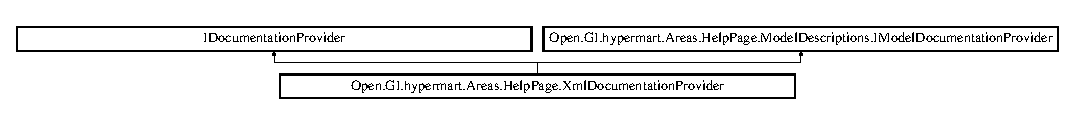
\includegraphics[height=1.102362cm]{class_open_1_1_g_i_1_1hypermart_1_1_areas_1_1_help_page_1_1_xml_documentation_provider}
\end{center}
\end{figure}
\subsection*{Public Member Functions}
\begin{DoxyCompactItemize}
\item 
\hyperlink{class_open_1_1_g_i_1_1hypermart_1_1_areas_1_1_help_page_1_1_xml_documentation_provider_a20855501bd3ff394652127b70e822308}{Xml\+Documentation\+Provider} (string document\+Path)
\begin{DoxyCompactList}\small\item\em Initializes a new instance of the \hyperlink{class_open_1_1_g_i_1_1hypermart_1_1_areas_1_1_help_page_1_1_xml_documentation_provider}{Xml\+Documentation\+Provider} class. \end{DoxyCompactList}\item 
string \hyperlink{class_open_1_1_g_i_1_1hypermart_1_1_areas_1_1_help_page_1_1_xml_documentation_provider_a05e11e0de4ff25a0e602ce9e5e916056}{Get\+Documentation} (Http\+Controller\+Descriptor controller\+Descriptor)
\begin{DoxyCompactList}\small\item\em Gets the documentation. \end{DoxyCompactList}\item 
virtual string \hyperlink{class_open_1_1_g_i_1_1hypermart_1_1_areas_1_1_help_page_1_1_xml_documentation_provider_ad27b3bee09fd9709d46eb720bff4b860}{Get\+Documentation} (Http\+Action\+Descriptor action\+Descriptor)
\begin{DoxyCompactList}\small\item\em Gets the documentation based on T\+:\+System.\+Web.\+Http.\+Controllers.\+Http\+Action\+Descriptor. \end{DoxyCompactList}\item 
virtual string \hyperlink{class_open_1_1_g_i_1_1hypermart_1_1_areas_1_1_help_page_1_1_xml_documentation_provider_a765e1ebc7e331274a664dd0edba7660c}{Get\+Documentation} (Http\+Parameter\+Descriptor parameter\+Descriptor)
\begin{DoxyCompactList}\small\item\em Gets the documentation based on T\+:\+System.\+Web.\+Http.\+Controllers.\+Http\+Parameter\+Descriptor. \end{DoxyCompactList}\item 
string \hyperlink{class_open_1_1_g_i_1_1hypermart_1_1_areas_1_1_help_page_1_1_xml_documentation_provider_a3f8e45cb0b20d0aef5e795a7ac638346}{Get\+Response\+Documentation} (Http\+Action\+Descriptor action\+Descriptor)
\begin{DoxyCompactList}\small\item\em Gets the response documentation. \end{DoxyCompactList}\item 
string \hyperlink{class_open_1_1_g_i_1_1hypermart_1_1_areas_1_1_help_page_1_1_xml_documentation_provider_a1ba7e50dea71787a555f92306ec99efc}{Get\+Documentation} (Member\+Info member)
\begin{DoxyCompactList}\small\item\em Gets the documentation. \end{DoxyCompactList}\item 
string \hyperlink{class_open_1_1_g_i_1_1hypermart_1_1_areas_1_1_help_page_1_1_xml_documentation_provider_af096939cdb4e5a26bd20ae3341fad66c}{Get\+Documentation} (Type type)
\begin{DoxyCompactList}\small\item\em Gets the documentation. \end{DoxyCompactList}\end{DoxyCompactItemize}


\subsection{Detailed Description}
A custom I\+Documentation\+Provider that reads the A\+P\+I documentation from an X\+M\+L documentation file. 



Definition at line 15 of file Xml\+Documentation\+Provider.\+cs.



\subsection{Constructor \& Destructor Documentation}
\hypertarget{class_open_1_1_g_i_1_1hypermart_1_1_areas_1_1_help_page_1_1_xml_documentation_provider_a20855501bd3ff394652127b70e822308}{}\index{Open\+::\+G\+I\+::hypermart\+::\+Areas\+::\+Help\+Page\+::\+Xml\+Documentation\+Provider@{Open\+::\+G\+I\+::hypermart\+::\+Areas\+::\+Help\+Page\+::\+Xml\+Documentation\+Provider}!Xml\+Documentation\+Provider@{Xml\+Documentation\+Provider}}
\index{Xml\+Documentation\+Provider@{Xml\+Documentation\+Provider}!Open\+::\+G\+I\+::hypermart\+::\+Areas\+::\+Help\+Page\+::\+Xml\+Documentation\+Provider@{Open\+::\+G\+I\+::hypermart\+::\+Areas\+::\+Help\+Page\+::\+Xml\+Documentation\+Provider}}
\subsubsection[{Xml\+Documentation\+Provider(string document\+Path)}]{\setlength{\rightskip}{0pt plus 5cm}Open.\+G\+I.\+hypermart.\+Areas.\+Help\+Page.\+Xml\+Documentation\+Provider.\+Xml\+Documentation\+Provider (
\begin{DoxyParamCaption}
\item[{string}]{document\+Path}
\end{DoxyParamCaption}
)}\label{class_open_1_1_g_i_1_1hypermart_1_1_areas_1_1_help_page_1_1_xml_documentation_provider_a20855501bd3ff394652127b70e822308}


Initializes a new instance of the \hyperlink{class_open_1_1_g_i_1_1hypermart_1_1_areas_1_1_help_page_1_1_xml_documentation_provider}{Xml\+Documentation\+Provider} class. 


\begin{DoxyParams}{Parameters}
{\em document\+Path} & The physical path to X\+M\+L document.\\
\hline
\end{DoxyParams}


Definition at line 28 of file Xml\+Documentation\+Provider.\+cs.



\subsection{Member Function Documentation}
\hypertarget{class_open_1_1_g_i_1_1hypermart_1_1_areas_1_1_help_page_1_1_xml_documentation_provider_a05e11e0de4ff25a0e602ce9e5e916056}{}\index{Open\+::\+G\+I\+::hypermart\+::\+Areas\+::\+Help\+Page\+::\+Xml\+Documentation\+Provider@{Open\+::\+G\+I\+::hypermart\+::\+Areas\+::\+Help\+Page\+::\+Xml\+Documentation\+Provider}!Get\+Documentation@{Get\+Documentation}}
\index{Get\+Documentation@{Get\+Documentation}!Open\+::\+G\+I\+::hypermart\+::\+Areas\+::\+Help\+Page\+::\+Xml\+Documentation\+Provider@{Open\+::\+G\+I\+::hypermart\+::\+Areas\+::\+Help\+Page\+::\+Xml\+Documentation\+Provider}}
\subsubsection[{Get\+Documentation(\+Http\+Controller\+Descriptor controller\+Descriptor)}]{\setlength{\rightskip}{0pt plus 5cm}string Open.\+G\+I.\+hypermart.\+Areas.\+Help\+Page.\+Xml\+Documentation\+Provider.\+Get\+Documentation (
\begin{DoxyParamCaption}
\item[{Http\+Controller\+Descriptor}]{controller\+Descriptor}
\end{DoxyParamCaption}
)}\label{class_open_1_1_g_i_1_1hypermart_1_1_areas_1_1_help_page_1_1_xml_documentation_provider_a05e11e0de4ff25a0e602ce9e5e916056}


Gets the documentation. 


\begin{DoxyParams}{Parameters}
{\em controller\+Descriptor} & The controller descriptor.\\
\hline
\end{DoxyParams}
\begin{DoxyReturn}{Returns}

\end{DoxyReturn}


Definition at line 43 of file Xml\+Documentation\+Provider.\+cs.

\hypertarget{class_open_1_1_g_i_1_1hypermart_1_1_areas_1_1_help_page_1_1_xml_documentation_provider_ad27b3bee09fd9709d46eb720bff4b860}{}\index{Open\+::\+G\+I\+::hypermart\+::\+Areas\+::\+Help\+Page\+::\+Xml\+Documentation\+Provider@{Open\+::\+G\+I\+::hypermart\+::\+Areas\+::\+Help\+Page\+::\+Xml\+Documentation\+Provider}!Get\+Documentation@{Get\+Documentation}}
\index{Get\+Documentation@{Get\+Documentation}!Open\+::\+G\+I\+::hypermart\+::\+Areas\+::\+Help\+Page\+::\+Xml\+Documentation\+Provider@{Open\+::\+G\+I\+::hypermart\+::\+Areas\+::\+Help\+Page\+::\+Xml\+Documentation\+Provider}}
\subsubsection[{Get\+Documentation(\+Http\+Action\+Descriptor action\+Descriptor)}]{\setlength{\rightskip}{0pt plus 5cm}virtual string Open.\+G\+I.\+hypermart.\+Areas.\+Help\+Page.\+Xml\+Documentation\+Provider.\+Get\+Documentation (
\begin{DoxyParamCaption}
\item[{Http\+Action\+Descriptor}]{action\+Descriptor}
\end{DoxyParamCaption}
)\hspace{0.3cm}{\ttfamily [virtual]}}\label{class_open_1_1_g_i_1_1hypermart_1_1_areas_1_1_help_page_1_1_xml_documentation_provider_ad27b3bee09fd9709d46eb720bff4b860}


Gets the documentation based on T\+:\+System.\+Web.\+Http.\+Controllers.\+Http\+Action\+Descriptor. 


\begin{DoxyParams}{Parameters}
{\em action\+Descriptor} & The action descriptor.\\
\hline
\end{DoxyParams}
\begin{DoxyReturn}{Returns}
The documentation for the controller. 
\end{DoxyReturn}


Definition at line 56 of file Xml\+Documentation\+Provider.\+cs.

\hypertarget{class_open_1_1_g_i_1_1hypermart_1_1_areas_1_1_help_page_1_1_xml_documentation_provider_a765e1ebc7e331274a664dd0edba7660c}{}\index{Open\+::\+G\+I\+::hypermart\+::\+Areas\+::\+Help\+Page\+::\+Xml\+Documentation\+Provider@{Open\+::\+G\+I\+::hypermart\+::\+Areas\+::\+Help\+Page\+::\+Xml\+Documentation\+Provider}!Get\+Documentation@{Get\+Documentation}}
\index{Get\+Documentation@{Get\+Documentation}!Open\+::\+G\+I\+::hypermart\+::\+Areas\+::\+Help\+Page\+::\+Xml\+Documentation\+Provider@{Open\+::\+G\+I\+::hypermart\+::\+Areas\+::\+Help\+Page\+::\+Xml\+Documentation\+Provider}}
\subsubsection[{Get\+Documentation(\+Http\+Parameter\+Descriptor parameter\+Descriptor)}]{\setlength{\rightskip}{0pt plus 5cm}virtual string Open.\+G\+I.\+hypermart.\+Areas.\+Help\+Page.\+Xml\+Documentation\+Provider.\+Get\+Documentation (
\begin{DoxyParamCaption}
\item[{Http\+Parameter\+Descriptor}]{parameter\+Descriptor}
\end{DoxyParamCaption}
)\hspace{0.3cm}{\ttfamily [virtual]}}\label{class_open_1_1_g_i_1_1hypermart_1_1_areas_1_1_help_page_1_1_xml_documentation_provider_a765e1ebc7e331274a664dd0edba7660c}


Gets the documentation based on T\+:\+System.\+Web.\+Http.\+Controllers.\+Http\+Parameter\+Descriptor. 


\begin{DoxyParams}{Parameters}
{\em parameter\+Descriptor} & The parameter descriptor.\\
\hline
\end{DoxyParams}
\begin{DoxyReturn}{Returns}
The documentation for the controller. 
\end{DoxyReturn}


Definition at line 69 of file Xml\+Documentation\+Provider.\+cs.

\hypertarget{class_open_1_1_g_i_1_1hypermart_1_1_areas_1_1_help_page_1_1_xml_documentation_provider_a1ba7e50dea71787a555f92306ec99efc}{}\index{Open\+::\+G\+I\+::hypermart\+::\+Areas\+::\+Help\+Page\+::\+Xml\+Documentation\+Provider@{Open\+::\+G\+I\+::hypermart\+::\+Areas\+::\+Help\+Page\+::\+Xml\+Documentation\+Provider}!Get\+Documentation@{Get\+Documentation}}
\index{Get\+Documentation@{Get\+Documentation}!Open\+::\+G\+I\+::hypermart\+::\+Areas\+::\+Help\+Page\+::\+Xml\+Documentation\+Provider@{Open\+::\+G\+I\+::hypermart\+::\+Areas\+::\+Help\+Page\+::\+Xml\+Documentation\+Provider}}
\subsubsection[{Get\+Documentation(\+Member\+Info member)}]{\setlength{\rightskip}{0pt plus 5cm}string Open.\+G\+I.\+hypermart.\+Areas.\+Help\+Page.\+Xml\+Documentation\+Provider.\+Get\+Documentation (
\begin{DoxyParamCaption}
\item[{Member\+Info}]{member}
\end{DoxyParamCaption}
)}\label{class_open_1_1_g_i_1_1hypermart_1_1_areas_1_1_help_page_1_1_xml_documentation_provider_a1ba7e50dea71787a555f92306ec99efc}


Gets the documentation. 


\begin{DoxyParams}{Parameters}
{\em member} & The member.\\
\hline
\end{DoxyParams}
\begin{DoxyReturn}{Returns}

\end{DoxyReturn}


Implements \hyperlink{interface_open_1_1_g_i_1_1hypermart_1_1_areas_1_1_help_page_1_1_model_descriptions_1_1_i_model_documentation_provider_a27d4470da05e52051ae345515c17755a}{Open.\+G\+I.\+hypermart.\+Areas.\+Help\+Page.\+Model\+Descriptions.\+I\+Model\+Documentation\+Provider}.



Definition at line 105 of file Xml\+Documentation\+Provider.\+cs.

\hypertarget{class_open_1_1_g_i_1_1hypermart_1_1_areas_1_1_help_page_1_1_xml_documentation_provider_af096939cdb4e5a26bd20ae3341fad66c}{}\index{Open\+::\+G\+I\+::hypermart\+::\+Areas\+::\+Help\+Page\+::\+Xml\+Documentation\+Provider@{Open\+::\+G\+I\+::hypermart\+::\+Areas\+::\+Help\+Page\+::\+Xml\+Documentation\+Provider}!Get\+Documentation@{Get\+Documentation}}
\index{Get\+Documentation@{Get\+Documentation}!Open\+::\+G\+I\+::hypermart\+::\+Areas\+::\+Help\+Page\+::\+Xml\+Documentation\+Provider@{Open\+::\+G\+I\+::hypermart\+::\+Areas\+::\+Help\+Page\+::\+Xml\+Documentation\+Provider}}
\subsubsection[{Get\+Documentation(\+Type type)}]{\setlength{\rightskip}{0pt plus 5cm}string Open.\+G\+I.\+hypermart.\+Areas.\+Help\+Page.\+Xml\+Documentation\+Provider.\+Get\+Documentation (
\begin{DoxyParamCaption}
\item[{Type}]{type}
\end{DoxyParamCaption}
)}\label{class_open_1_1_g_i_1_1hypermart_1_1_areas_1_1_help_page_1_1_xml_documentation_provider_af096939cdb4e5a26bd20ae3341fad66c}


Gets the documentation. 


\begin{DoxyParams}{Parameters}
{\em type} & The type.\\
\hline
\end{DoxyParams}
\begin{DoxyReturn}{Returns}

\end{DoxyReturn}


Implements \hyperlink{interface_open_1_1_g_i_1_1hypermart_1_1_areas_1_1_help_page_1_1_model_descriptions_1_1_i_model_documentation_provider_a047061b90c62930fc0a1dbcb09732bd3}{Open.\+G\+I.\+hypermart.\+Areas.\+Help\+Page.\+Model\+Descriptions.\+I\+Model\+Documentation\+Provider}.



Definition at line 119 of file Xml\+Documentation\+Provider.\+cs.

\hypertarget{class_open_1_1_g_i_1_1hypermart_1_1_areas_1_1_help_page_1_1_xml_documentation_provider_a3f8e45cb0b20d0aef5e795a7ac638346}{}\index{Open\+::\+G\+I\+::hypermart\+::\+Areas\+::\+Help\+Page\+::\+Xml\+Documentation\+Provider@{Open\+::\+G\+I\+::hypermart\+::\+Areas\+::\+Help\+Page\+::\+Xml\+Documentation\+Provider}!Get\+Response\+Documentation@{Get\+Response\+Documentation}}
\index{Get\+Response\+Documentation@{Get\+Response\+Documentation}!Open\+::\+G\+I\+::hypermart\+::\+Areas\+::\+Help\+Page\+::\+Xml\+Documentation\+Provider@{Open\+::\+G\+I\+::hypermart\+::\+Areas\+::\+Help\+Page\+::\+Xml\+Documentation\+Provider}}
\subsubsection[{Get\+Response\+Documentation(\+Http\+Action\+Descriptor action\+Descriptor)}]{\setlength{\rightskip}{0pt plus 5cm}string Open.\+G\+I.\+hypermart.\+Areas.\+Help\+Page.\+Xml\+Documentation\+Provider.\+Get\+Response\+Documentation (
\begin{DoxyParamCaption}
\item[{Http\+Action\+Descriptor}]{action\+Descriptor}
\end{DoxyParamCaption}
)}\label{class_open_1_1_g_i_1_1hypermart_1_1_areas_1_1_help_page_1_1_xml_documentation_provider_a3f8e45cb0b20d0aef5e795a7ac638346}


Gets the response documentation. 


\begin{DoxyParams}{Parameters}
{\em action\+Descriptor} & The action descriptor.\\
\hline
\end{DoxyParams}
\begin{DoxyReturn}{Returns}

\end{DoxyReturn}


Definition at line 94 of file Xml\+Documentation\+Provider.\+cs.



The documentation for this class was generated from the following file\+:\begin{DoxyCompactItemize}
\item 
C\+:/\+Projects/\+App-\/\+Utility-\/\+Store/\+Open.\+G\+I.\+hypermart/\+Areas/\+Help\+Page/\hyperlink{_xml_documentation_provider_8cs}{Xml\+Documentation\+Provider.\+cs}\end{DoxyCompactItemize}

\chapter{File Documentation}
\hypertarget{_bundle_config_8cs}{}\section{C\+:/\+Projects/\+App-\/\+Utility-\/\+Store/\+Open.G\+I.\+hypermart/\+App\+\_\+\+Start/\+Bundle\+Config.cs File Reference}
\label{_bundle_config_8cs}\index{C\+:/\+Projects/\+App-\/\+Utility-\/\+Store/\+Open.\+G\+I.\+hypermart/\+App\+\_\+\+Start/\+Bundle\+Config.\+cs@{C\+:/\+Projects/\+App-\/\+Utility-\/\+Store/\+Open.\+G\+I.\+hypermart/\+App\+\_\+\+Start/\+Bundle\+Config.\+cs}}
\subsection*{Classes}
\begin{DoxyCompactItemize}
\item 
class \hyperlink{class_open_1_1_g_i_1_1hypermart_1_1_bundle_config}{Open.\+G\+I.\+hypermart.\+Bundle\+Config}
\begin{DoxyCompactList}\small\item\em A\+S\+P.\+N\+E\+T M\+V\+C Bundle configuration \end{DoxyCompactList}\end{DoxyCompactItemize}
\subsection*{Namespaces}
\begin{DoxyCompactItemize}
\item 
namespace \hyperlink{namespace_open_1_1_g_i_1_1hypermart}{Open.\+G\+I.\+hypermart}
\end{DoxyCompactItemize}

\section{C\+:/\+Projects/\+App-\/\+Utility-\/\+Store/\+Open.G\+I.\+hypermart/\+App\+\_\+\+Start/\+Filter\+Config.cs File Reference}
\label{_filter_config_8cs}\index{C\+:/\+Projects/\+App-\/\+Utility-\/\+Store/\+Open.\+G\+I.\+hypermart/\+App\+\_\+\+Start/\+Filter\+Config.\+cs@{C\+:/\+Projects/\+App-\/\+Utility-\/\+Store/\+Open.\+G\+I.\+hypermart/\+App\+\_\+\+Start/\+Filter\+Config.\+cs}}
\subsection*{Classes}
\begin{DoxyCompactItemize}
\item 
class \textbf{ Open.\+G\+I.\+hypermart.\+Filter\+Config}
\begin{DoxyCompactList}\small\item\em Class for filter configuration \end{DoxyCompactList}\end{DoxyCompactItemize}
\subsection*{Namespaces}
\begin{DoxyCompactItemize}
\item 
namespace \textbf{ Open.\+G\+I.\+hypermart}
\end{DoxyCompactItemize}

\hypertarget{_route_config_8cs}{}\section{C\+:/\+Projects/\+App-\/\+Utility-\/\+Store/\+Open.G\+I.\+hypermart/\+App\+\_\+\+Start/\+Route\+Config.cs File Reference}
\label{_route_config_8cs}\index{C\+:/\+Projects/\+App-\/\+Utility-\/\+Store/\+Open.\+G\+I.\+hypermart/\+App\+\_\+\+Start/\+Route\+Config.\+cs@{C\+:/\+Projects/\+App-\/\+Utility-\/\+Store/\+Open.\+G\+I.\+hypermart/\+App\+\_\+\+Start/\+Route\+Config.\+cs}}
\subsection*{Classes}
\begin{DoxyCompactItemize}
\item 
class \hyperlink{class_open_1_1_g_i_1_1hypermart_1_1_route_config}{Open.\+G\+I.\+hypermart.\+Route\+Config}
\begin{DoxyCompactList}\small\item\em M\+VC -\/ Route Registration \end{DoxyCompactList}\end{DoxyCompactItemize}
\subsection*{Namespaces}
\begin{DoxyCompactItemize}
\item 
namespace \hyperlink{namespace_open_1_1_g_i_1_1hypermart}{Open.\+G\+I.\+hypermart}
\end{DoxyCompactItemize}

\section{C\+:/\+Projects/\+App-\/\+Utility-\/\+Store/\+Open.G\+I.\+hypermart/\+App\+\_\+\+Start/\+Unity\+Config.cs File Reference}
\label{_unity_config_8cs}\index{C\+:/\+Projects/\+App-\/\+Utility-\/\+Store/\+Open.\+G\+I.\+hypermart/\+App\+\_\+\+Start/\+Unity\+Config.\+cs@{C\+:/\+Projects/\+App-\/\+Utility-\/\+Store/\+Open.\+G\+I.\+hypermart/\+App\+\_\+\+Start/\+Unity\+Config.\+cs}}
\subsection*{Classes}
\begin{DoxyCompactItemize}
\item 
class \textbf{ Open.\+G\+I.\+hypermart.\+App\+\_\+\+Start.\+Unity\+Config}
\begin{DoxyCompactList}\small\item\em Specifies the Unity configuration for the main container. \end{DoxyCompactList}\end{DoxyCompactItemize}
\subsection*{Namespaces}
\begin{DoxyCompactItemize}
\item 
namespace \textbf{ Open.\+G\+I.\+hypermart.\+App\+\_\+\+Start}
\end{DoxyCompactItemize}

\hypertarget{_unity_mvc_activator_8cs}{}\section{C\+:/\+Projects/\+App-\/\+Utility-\/\+Store/\+Open.G\+I.\+hypermart/\+App\+\_\+\+Start/\+Unity\+Mvc\+Activator.cs File Reference}
\label{_unity_mvc_activator_8cs}\index{C\+:/\+Projects/\+App-\/\+Utility-\/\+Store/\+Open.\+G\+I.\+hypermart/\+App\+\_\+\+Start/\+Unity\+Mvc\+Activator.\+cs@{C\+:/\+Projects/\+App-\/\+Utility-\/\+Store/\+Open.\+G\+I.\+hypermart/\+App\+\_\+\+Start/\+Unity\+Mvc\+Activator.\+cs}}
\subsection*{Classes}
\begin{DoxyCompactItemize}
\item 
class {\bfseries Open.\+G\+I.\+hypermart.\+App\+\_\+\+Start.\+Unity\+Web\+Activator}
\begin{DoxyCompactList}\small\item\em Provides the bootstrapping for integrating Unity with A\+S\+P.\+N\+ET M\+VC.\end{DoxyCompactList}\end{DoxyCompactItemize}
\subsection*{Namespaces}
\begin{DoxyCompactItemize}
\item 
namespace \hyperlink{namespace_open_1_1_g_i_1_1hypermart_1_1_app___start}{Open.\+G\+I.\+hypermart.\+App\+\_\+\+Start}
\end{DoxyCompactItemize}

\section{C\+:/\+Projects/\+App-\/\+Utility-\/\+Store/\+Open.G\+I.\+hypermart/\+App\+\_\+\+Start/\+Web\+Api\+Config.cs File Reference}
\label{_web_api_config_8cs}\index{C\+:/\+Projects/\+App-\/\+Utility-\/\+Store/\+Open.\+G\+I.\+hypermart/\+App\+\_\+\+Start/\+Web\+Api\+Config.\+cs@{C\+:/\+Projects/\+App-\/\+Utility-\/\+Store/\+Open.\+G\+I.\+hypermart/\+App\+\_\+\+Start/\+Web\+Api\+Config.\+cs}}
\subsection*{Classes}
\begin{DoxyCompactItemize}
\item 
class {\bfseries Open.\+G\+I.\+hypermart.\+Web\+Api\+Config}
\begin{DoxyCompactList}\small\item\em Configuring Web A\+PI layer \end{DoxyCompactList}\end{DoxyCompactItemize}
\subsection*{Namespaces}
\begin{DoxyCompactItemize}
\item 
namespace \textbf{ Open.\+G\+I.\+hypermart}
\end{DoxyCompactItemize}

\section{C\+:/\+Projects/\+App-\/\+Utility-\/\+Store/\+Open.G\+I.\+hypermart/\+Areas/\+Help\+Page/\+Api\+Description\+Extensions.cs File Reference}
\label{_api_description_extensions_8cs}\index{C\+:/\+Projects/\+App-\/\+Utility-\/\+Store/\+Open.\+G\+I.\+hypermart/\+Areas/\+Help\+Page/\+Api\+Description\+Extensions.\+cs@{C\+:/\+Projects/\+App-\/\+Utility-\/\+Store/\+Open.\+G\+I.\+hypermart/\+Areas/\+Help\+Page/\+Api\+Description\+Extensions.\+cs}}
\subsection*{Classes}
\begin{DoxyCompactItemize}
\item 
class {\bfseries Open.\+G\+I.\+hypermart.\+Areas.\+Help\+Page.\+Api\+Description\+Extensions}
\end{DoxyCompactItemize}
\subsection*{Namespaces}
\begin{DoxyCompactItemize}
\item 
namespace \textbf{ Open.\+G\+I.\+hypermart.\+Areas.\+Help\+Page}
\end{DoxyCompactItemize}

\hypertarget{_help_page_config_8cs}{}\section{C\+:/\+Projects/\+App-\/\+Utility-\/\+Store/\+Open.G\+I.\+hypermart/\+Areas/\+Help\+Page/\+App\+\_\+\+Start/\+Help\+Page\+Config.cs File Reference}
\label{_help_page_config_8cs}\index{C\+:/\+Projects/\+App-\/\+Utility-\/\+Store/\+Open.\+G\+I.\+hypermart/\+Areas/\+Help\+Page/\+App\+\_\+\+Start/\+Help\+Page\+Config.\+cs@{C\+:/\+Projects/\+App-\/\+Utility-\/\+Store/\+Open.\+G\+I.\+hypermart/\+Areas/\+Help\+Page/\+App\+\_\+\+Start/\+Help\+Page\+Config.\+cs}}
\subsection*{Classes}
\begin{DoxyCompactItemize}
\item 
class {\bfseries Open.\+G\+I.\+hypermart.\+Areas.\+Help\+Page.\+Help\+Page\+Config}
\begin{DoxyCompactList}\small\item\em Use this class to customize the Help Page. For example you can set a custom System.\+Web.\+Http.\+Description.\+I\+Documentation\+Provider to supply the documentation or you can provide the samples for the requests/responses. \end{DoxyCompactList}\end{DoxyCompactItemize}
\subsection*{Namespaces}
\begin{DoxyCompactItemize}
\item 
namespace \hyperlink{namespace_open_1_1_g_i_1_1hypermart_1_1_areas_1_1_help_page}{Open.\+G\+I.\+hypermart.\+Areas.\+Help\+Page}
\end{DoxyCompactItemize}

\section{C\+:/\+Projects/\+App-\/\+Utility-\/\+Store/\+Open.G\+I.\+hypermart/\+Areas/\+Help\+Page/\+Controllers/\+Help\+Controller.cs File Reference}
\label{_help_controller_8cs}\index{C\+:/\+Projects/\+App-\/\+Utility-\/\+Store/\+Open.\+G\+I.\+hypermart/\+Areas/\+Help\+Page/\+Controllers/\+Help\+Controller.\+cs@{C\+:/\+Projects/\+App-\/\+Utility-\/\+Store/\+Open.\+G\+I.\+hypermart/\+Areas/\+Help\+Page/\+Controllers/\+Help\+Controller.\+cs}}
\subsection*{Classes}
\begin{DoxyCompactItemize}
\item 
class \textbf{ Open.\+G\+I.\+hypermart.\+Areas.\+Help\+Page.\+Controllers.\+Help\+Controller}
\begin{DoxyCompactList}\small\item\em The controller that will handle requests for the help page. \end{DoxyCompactList}\end{DoxyCompactItemize}
\subsection*{Namespaces}
\begin{DoxyCompactItemize}
\item 
namespace \textbf{ Open.\+G\+I.\+hypermart.\+Areas.\+Help\+Page.\+Controllers}
\end{DoxyCompactItemize}

\section{C\+:/\+Projects/\+App-\/\+Utility-\/\+Store/\+Open.G\+I.\+hypermart/\+Areas/\+Help\+Page/\+Help\+Page\+Area\+Registration.cs File Reference}
\label{_help_page_area_registration_8cs}\index{C\+:/\+Projects/\+App-\/\+Utility-\/\+Store/\+Open.\+G\+I.\+hypermart/\+Areas/\+Help\+Page/\+Help\+Page\+Area\+Registration.\+cs@{C\+:/\+Projects/\+App-\/\+Utility-\/\+Store/\+Open.\+G\+I.\+hypermart/\+Areas/\+Help\+Page/\+Help\+Page\+Area\+Registration.\+cs}}
\subsection*{Classes}
\begin{DoxyCompactItemize}
\item 
class \textbf{ Open.\+G\+I.\+hypermart.\+Areas.\+Help\+Page.\+Help\+Page\+Area\+Registration}
\end{DoxyCompactItemize}
\subsection*{Namespaces}
\begin{DoxyCompactItemize}
\item 
namespace \textbf{ Open.\+G\+I.\+hypermart.\+Areas.\+Help\+Page}
\end{DoxyCompactItemize}

\section{C\+:/\+Projects/\+App-\/\+Utility-\/\+Store/\+Open.G\+I.\+hypermart/\+Areas/\+Help\+Page/\+Help\+Page\+Configuration\+Extensions.cs File Reference}
\label{_help_page_configuration_extensions_8cs}\index{C\+:/\+Projects/\+App-\/\+Utility-\/\+Store/\+Open.\+G\+I.\+hypermart/\+Areas/\+Help\+Page/\+Help\+Page\+Configuration\+Extensions.\+cs@{C\+:/\+Projects/\+App-\/\+Utility-\/\+Store/\+Open.\+G\+I.\+hypermart/\+Areas/\+Help\+Page/\+Help\+Page\+Configuration\+Extensions.\+cs}}
\subsection*{Classes}
\begin{DoxyCompactItemize}
\item 
class {\bfseries Open.\+G\+I.\+hypermart.\+Areas.\+Help\+Page.\+Help\+Page\+Configuration\+Extensions}
\end{DoxyCompactItemize}
\subsection*{Namespaces}
\begin{DoxyCompactItemize}
\item 
namespace \textbf{ Open.\+G\+I.\+hypermart.\+Areas.\+Help\+Page}
\end{DoxyCompactItemize}

\section{C\+:/\+Projects/\+App-\/\+Utility-\/\+Store/\+Open.G\+I.\+hypermart/\+Areas/\+Help\+Page/\+Model\+Descriptions/\+Collection\+Model\+Description.cs File Reference}
\label{_collection_model_description_8cs}\index{C\+:/\+Projects/\+App-\/\+Utility-\/\+Store/\+Open.\+G\+I.\+hypermart/\+Areas/\+Help\+Page/\+Model\+Descriptions/\+Collection\+Model\+Description.\+cs@{C\+:/\+Projects/\+App-\/\+Utility-\/\+Store/\+Open.\+G\+I.\+hypermart/\+Areas/\+Help\+Page/\+Model\+Descriptions/\+Collection\+Model\+Description.\+cs}}
\subsection*{Classes}
\begin{DoxyCompactItemize}
\item 
class \textbf{ Open.\+G\+I.\+hypermart.\+Areas.\+Help\+Page.\+Model\+Descriptions.\+Collection\+Model\+Description}
\end{DoxyCompactItemize}
\subsection*{Namespaces}
\begin{DoxyCompactItemize}
\item 
namespace \textbf{ Open.\+G\+I.\+hypermart.\+Areas.\+Help\+Page.\+Model\+Descriptions}
\end{DoxyCompactItemize}

\hypertarget{_complex_type_model_description_8cs}{}\section{C\+:/\+Projects/\+App-\/\+Utility-\/\+Store/\+Open.G\+I.\+hypermart/\+Areas/\+Help\+Page/\+Model\+Descriptions/\+Complex\+Type\+Model\+Description.cs File Reference}
\label{_complex_type_model_description_8cs}\index{C\+:/\+Projects/\+App-\/\+Utility-\/\+Store/\+Open.\+G\+I.\+hypermart/\+Areas/\+Help\+Page/\+Model\+Descriptions/\+Complex\+Type\+Model\+Description.\+cs@{C\+:/\+Projects/\+App-\/\+Utility-\/\+Store/\+Open.\+G\+I.\+hypermart/\+Areas/\+Help\+Page/\+Model\+Descriptions/\+Complex\+Type\+Model\+Description.\+cs}}
\subsection*{Classes}
\begin{DoxyCompactItemize}
\item 
class \hyperlink{class_open_1_1_g_i_1_1hypermart_1_1_areas_1_1_help_page_1_1_model_descriptions_1_1_complex_type_model_description}{Open.\+G\+I.\+hypermart.\+Areas.\+Help\+Page.\+Model\+Descriptions.\+Complex\+Type\+Model\+Description}
\end{DoxyCompactItemize}
\subsection*{Namespaces}
\begin{DoxyCompactItemize}
\item 
namespace \hyperlink{namespace_open_1_1_g_i_1_1hypermart_1_1_areas_1_1_help_page_1_1_model_descriptions}{Open.\+G\+I.\+hypermart.\+Areas.\+Help\+Page.\+Model\+Descriptions}
\end{DoxyCompactItemize}

\hypertarget{_dictionary_model_description_8cs}{}\section{C\+:/\+Projects/\+App-\/\+Utility-\/\+Store/\+Open.G\+I.\+hypermart/\+Areas/\+Help\+Page/\+Model\+Descriptions/\+Dictionary\+Model\+Description.cs File Reference}
\label{_dictionary_model_description_8cs}\index{C\+:/\+Projects/\+App-\/\+Utility-\/\+Store/\+Open.\+G\+I.\+hypermart/\+Areas/\+Help\+Page/\+Model\+Descriptions/\+Dictionary\+Model\+Description.\+cs@{C\+:/\+Projects/\+App-\/\+Utility-\/\+Store/\+Open.\+G\+I.\+hypermart/\+Areas/\+Help\+Page/\+Model\+Descriptions/\+Dictionary\+Model\+Description.\+cs}}
\subsection*{Classes}
\begin{DoxyCompactItemize}
\item 
class \hyperlink{class_open_1_1_g_i_1_1hypermart_1_1_areas_1_1_help_page_1_1_model_descriptions_1_1_dictionary_model_description}{Open.\+G\+I.\+hypermart.\+Areas.\+Help\+Page.\+Model\+Descriptions.\+Dictionary\+Model\+Description}
\end{DoxyCompactItemize}
\subsection*{Namespaces}
\begin{DoxyCompactItemize}
\item 
namespace \hyperlink{namespace_open_1_1_g_i_1_1hypermart_1_1_areas_1_1_help_page_1_1_model_descriptions}{Open.\+G\+I.\+hypermart.\+Areas.\+Help\+Page.\+Model\+Descriptions}
\end{DoxyCompactItemize}

\section{C\+:/\+Projects/\+App-\/\+Utility-\/\+Store/\+Open.G\+I.\+hypermart/\+Areas/\+Help\+Page/\+Model\+Descriptions/\+Enum\+Type\+Model\+Description.cs File Reference}
\label{_enum_type_model_description_8cs}\index{C\+:/\+Projects/\+App-\/\+Utility-\/\+Store/\+Open.\+G\+I.\+hypermart/\+Areas/\+Help\+Page/\+Model\+Descriptions/\+Enum\+Type\+Model\+Description.\+cs@{C\+:/\+Projects/\+App-\/\+Utility-\/\+Store/\+Open.\+G\+I.\+hypermart/\+Areas/\+Help\+Page/\+Model\+Descriptions/\+Enum\+Type\+Model\+Description.\+cs}}
\subsection*{Classes}
\begin{DoxyCompactItemize}
\item 
class \textbf{ Open.\+G\+I.\+hypermart.\+Areas.\+Help\+Page.\+Model\+Descriptions.\+Enum\+Type\+Model\+Description}
\end{DoxyCompactItemize}
\subsection*{Namespaces}
\begin{DoxyCompactItemize}
\item 
namespace \textbf{ Open.\+G\+I.\+hypermart.\+Areas.\+Help\+Page.\+Model\+Descriptions}
\end{DoxyCompactItemize}

\section{C\+:/\+Projects/\+App-\/\+Utility-\/\+Store/\+Open.G\+I.\+hypermart/\+Areas/\+Help\+Page/\+Model\+Descriptions/\+Enum\+Value\+Description.cs File Reference}
\label{_enum_value_description_8cs}\index{C\+:/\+Projects/\+App-\/\+Utility-\/\+Store/\+Open.\+G\+I.\+hypermart/\+Areas/\+Help\+Page/\+Model\+Descriptions/\+Enum\+Value\+Description.\+cs@{C\+:/\+Projects/\+App-\/\+Utility-\/\+Store/\+Open.\+G\+I.\+hypermart/\+Areas/\+Help\+Page/\+Model\+Descriptions/\+Enum\+Value\+Description.\+cs}}
\subsection*{Classes}
\begin{DoxyCompactItemize}
\item 
class \textbf{ Open.\+G\+I.\+hypermart.\+Areas.\+Help\+Page.\+Model\+Descriptions.\+Enum\+Value\+Description}
\end{DoxyCompactItemize}
\subsection*{Namespaces}
\begin{DoxyCompactItemize}
\item 
namespace \textbf{ Open.\+G\+I.\+hypermart.\+Areas.\+Help\+Page.\+Model\+Descriptions}
\end{DoxyCompactItemize}

\hypertarget{_i_model_documentation_provider_8cs}{}\section{C\+:/\+Projects/\+App-\/\+Utility-\/\+Store/\+Open.G\+I.\+hypermart/\+Areas/\+Help\+Page/\+Model\+Descriptions/\+I\+Model\+Documentation\+Provider.cs File Reference}
\label{_i_model_documentation_provider_8cs}\index{C\+:/\+Projects/\+App-\/\+Utility-\/\+Store/\+Open.\+G\+I.\+hypermart/\+Areas/\+Help\+Page/\+Model\+Descriptions/\+I\+Model\+Documentation\+Provider.\+cs@{C\+:/\+Projects/\+App-\/\+Utility-\/\+Store/\+Open.\+G\+I.\+hypermart/\+Areas/\+Help\+Page/\+Model\+Descriptions/\+I\+Model\+Documentation\+Provider.\+cs}}
\subsection*{Classes}
\begin{DoxyCompactItemize}
\item 
interface \hyperlink{interface_open_1_1_g_i_1_1hypermart_1_1_areas_1_1_help_page_1_1_model_descriptions_1_1_i_model_documentation_provider}{Open.\+G\+I.\+hypermart.\+Areas.\+Help\+Page.\+Model\+Descriptions.\+I\+Model\+Documentation\+Provider}
\end{DoxyCompactItemize}
\subsection*{Namespaces}
\begin{DoxyCompactItemize}
\item 
namespace \hyperlink{namespace_open_1_1_g_i_1_1hypermart_1_1_areas_1_1_help_page_1_1_model_descriptions}{Open.\+G\+I.\+hypermart.\+Areas.\+Help\+Page.\+Model\+Descriptions}
\end{DoxyCompactItemize}

\section{C\+:/\+Projects/\+App-\/\+Utility-\/\+Store/\+Open.G\+I.\+hypermart/\+Areas/\+Help\+Page/\+Model\+Descriptions/\+Key\+Value\+Pair\+Model\+Description.cs File Reference}
\label{_key_value_pair_model_description_8cs}\index{C\+:/\+Projects/\+App-\/\+Utility-\/\+Store/\+Open.\+G\+I.\+hypermart/\+Areas/\+Help\+Page/\+Model\+Descriptions/\+Key\+Value\+Pair\+Model\+Description.\+cs@{C\+:/\+Projects/\+App-\/\+Utility-\/\+Store/\+Open.\+G\+I.\+hypermart/\+Areas/\+Help\+Page/\+Model\+Descriptions/\+Key\+Value\+Pair\+Model\+Description.\+cs}}
\subsection*{Classes}
\begin{DoxyCompactItemize}
\item 
class \textbf{ Open.\+G\+I.\+hypermart.\+Areas.\+Help\+Page.\+Model\+Descriptions.\+Key\+Value\+Pair\+Model\+Description}
\end{DoxyCompactItemize}
\subsection*{Namespaces}
\begin{DoxyCompactItemize}
\item 
namespace \textbf{ Open.\+G\+I.\+hypermart.\+Areas.\+Help\+Page.\+Model\+Descriptions}
\end{DoxyCompactItemize}

\hypertarget{_model_description_8cs}{}\section{C\+:/\+Projects/\+App-\/\+Utility-\/\+Store/\+Open.G\+I.\+hypermart/\+Areas/\+Help\+Page/\+Model\+Descriptions/\+Model\+Description.cs File Reference}
\label{_model_description_8cs}\index{C\+:/\+Projects/\+App-\/\+Utility-\/\+Store/\+Open.\+G\+I.\+hypermart/\+Areas/\+Help\+Page/\+Model\+Descriptions/\+Model\+Description.\+cs@{C\+:/\+Projects/\+App-\/\+Utility-\/\+Store/\+Open.\+G\+I.\+hypermart/\+Areas/\+Help\+Page/\+Model\+Descriptions/\+Model\+Description.\+cs}}
\subsection*{Classes}
\begin{DoxyCompactItemize}
\item 
class \hyperlink{class_open_1_1_g_i_1_1hypermart_1_1_areas_1_1_help_page_1_1_model_descriptions_1_1_model_description}{Open.\+G\+I.\+hypermart.\+Areas.\+Help\+Page.\+Model\+Descriptions.\+Model\+Description}
\begin{DoxyCompactList}\small\item\em Describes a type model. \end{DoxyCompactList}\end{DoxyCompactItemize}
\subsection*{Namespaces}
\begin{DoxyCompactItemize}
\item 
namespace \hyperlink{namespace_open_1_1_g_i_1_1hypermart_1_1_areas_1_1_help_page_1_1_model_descriptions}{Open.\+G\+I.\+hypermart.\+Areas.\+Help\+Page.\+Model\+Descriptions}
\end{DoxyCompactItemize}

\section{C\+:/\+Projects/\+App-\/\+Utility-\/\+Store/\+Open.G\+I.\+hypermart/\+Areas/\+Help\+Page/\+Model\+Descriptions/\+Model\+Description\+Generator.cs File Reference}
\label{_model_description_generator_8cs}\index{C\+:/\+Projects/\+App-\/\+Utility-\/\+Store/\+Open.\+G\+I.\+hypermart/\+Areas/\+Help\+Page/\+Model\+Descriptions/\+Model\+Description\+Generator.\+cs@{C\+:/\+Projects/\+App-\/\+Utility-\/\+Store/\+Open.\+G\+I.\+hypermart/\+Areas/\+Help\+Page/\+Model\+Descriptions/\+Model\+Description\+Generator.\+cs}}
\subsection*{Classes}
\begin{DoxyCompactItemize}
\item 
class \textbf{ Open.\+G\+I.\+hypermart.\+Areas.\+Help\+Page.\+Model\+Descriptions.\+Model\+Description\+Generator}
\begin{DoxyCompactList}\small\item\em Generates model descriptions for given types. \end{DoxyCompactList}\end{DoxyCompactItemize}
\subsection*{Namespaces}
\begin{DoxyCompactItemize}
\item 
namespace \textbf{ Open.\+G\+I.\+hypermart.\+Areas.\+Help\+Page.\+Model\+Descriptions}
\end{DoxyCompactItemize}

\hypertarget{_model_name_attribute_8cs}{}\section{C\+:/\+Projects/\+App-\/\+Utility-\/\+Store/\+Open.G\+I.\+hypermart/\+Areas/\+Help\+Page/\+Model\+Descriptions/\+Model\+Name\+Attribute.cs File Reference}
\label{_model_name_attribute_8cs}\index{C\+:/\+Projects/\+App-\/\+Utility-\/\+Store/\+Open.\+G\+I.\+hypermart/\+Areas/\+Help\+Page/\+Model\+Descriptions/\+Model\+Name\+Attribute.\+cs@{C\+:/\+Projects/\+App-\/\+Utility-\/\+Store/\+Open.\+G\+I.\+hypermart/\+Areas/\+Help\+Page/\+Model\+Descriptions/\+Model\+Name\+Attribute.\+cs}}
\subsection*{Classes}
\begin{DoxyCompactItemize}
\item 
class \hyperlink{class_open_1_1_g_i_1_1hypermart_1_1_areas_1_1_help_page_1_1_model_descriptions_1_1_model_name_attribute}{Open.\+G\+I.\+hypermart.\+Areas.\+Help\+Page.\+Model\+Descriptions.\+Model\+Name\+Attribute}
\begin{DoxyCompactList}\small\item\em Use this attribute to change the name of the \hyperlink{class_open_1_1_g_i_1_1hypermart_1_1_areas_1_1_help_page_1_1_model_descriptions_1_1_model_description}{Model\+Description} generated for a type. \end{DoxyCompactList}\end{DoxyCompactItemize}
\subsection*{Namespaces}
\begin{DoxyCompactItemize}
\item 
namespace \hyperlink{namespace_open_1_1_g_i_1_1hypermart_1_1_areas_1_1_help_page_1_1_model_descriptions}{Open.\+G\+I.\+hypermart.\+Areas.\+Help\+Page.\+Model\+Descriptions}
\end{DoxyCompactItemize}

\hypertarget{_model_name_helper_8cs}{}\section{C\+:/\+Projects/\+App-\/\+Utility-\/\+Store/\+Open.G\+I.\+hypermart/\+Areas/\+Help\+Page/\+Model\+Descriptions/\+Model\+Name\+Helper.cs File Reference}
\label{_model_name_helper_8cs}\index{C\+:/\+Projects/\+App-\/\+Utility-\/\+Store/\+Open.\+G\+I.\+hypermart/\+Areas/\+Help\+Page/\+Model\+Descriptions/\+Model\+Name\+Helper.\+cs@{C\+:/\+Projects/\+App-\/\+Utility-\/\+Store/\+Open.\+G\+I.\+hypermart/\+Areas/\+Help\+Page/\+Model\+Descriptions/\+Model\+Name\+Helper.\+cs}}
\subsection*{Classes}
\begin{DoxyCompactItemize}
\item 
class {\bfseries Open.\+G\+I.\+hypermart.\+Areas.\+Help\+Page.\+Model\+Descriptions.\+Model\+Name\+Helper}
\end{DoxyCompactItemize}
\subsection*{Namespaces}
\begin{DoxyCompactItemize}
\item 
namespace \hyperlink{namespace_open_1_1_g_i_1_1hypermart_1_1_areas_1_1_help_page_1_1_model_descriptions}{Open.\+G\+I.\+hypermart.\+Areas.\+Help\+Page.\+Model\+Descriptions}
\end{DoxyCompactItemize}

\hypertarget{_parameter_annotation_8cs}{}\section{C\+:/\+Projects/\+App-\/\+Utility-\/\+Store/\+Open.G\+I.\+hypermart/\+Areas/\+Help\+Page/\+Model\+Descriptions/\+Parameter\+Annotation.cs File Reference}
\label{_parameter_annotation_8cs}\index{C\+:/\+Projects/\+App-\/\+Utility-\/\+Store/\+Open.\+G\+I.\+hypermart/\+Areas/\+Help\+Page/\+Model\+Descriptions/\+Parameter\+Annotation.\+cs@{C\+:/\+Projects/\+App-\/\+Utility-\/\+Store/\+Open.\+G\+I.\+hypermart/\+Areas/\+Help\+Page/\+Model\+Descriptions/\+Parameter\+Annotation.\+cs}}
\subsection*{Classes}
\begin{DoxyCompactItemize}
\item 
class \hyperlink{class_open_1_1_g_i_1_1hypermart_1_1_areas_1_1_help_page_1_1_model_descriptions_1_1_parameter_annotation}{Open.\+G\+I.\+hypermart.\+Areas.\+Help\+Page.\+Model\+Descriptions.\+Parameter\+Annotation}
\end{DoxyCompactItemize}
\subsection*{Namespaces}
\begin{DoxyCompactItemize}
\item 
namespace \hyperlink{namespace_open_1_1_g_i_1_1hypermart_1_1_areas_1_1_help_page_1_1_model_descriptions}{Open.\+G\+I.\+hypermart.\+Areas.\+Help\+Page.\+Model\+Descriptions}
\end{DoxyCompactItemize}

\hypertarget{_parameter_description_8cs}{}\section{C\+:/\+Projects/\+App-\/\+Utility-\/\+Store/\+Open.G\+I.\+hypermart/\+Areas/\+Help\+Page/\+Model\+Descriptions/\+Parameter\+Description.cs File Reference}
\label{_parameter_description_8cs}\index{C\+:/\+Projects/\+App-\/\+Utility-\/\+Store/\+Open.\+G\+I.\+hypermart/\+Areas/\+Help\+Page/\+Model\+Descriptions/\+Parameter\+Description.\+cs@{C\+:/\+Projects/\+App-\/\+Utility-\/\+Store/\+Open.\+G\+I.\+hypermart/\+Areas/\+Help\+Page/\+Model\+Descriptions/\+Parameter\+Description.\+cs}}
\subsection*{Classes}
\begin{DoxyCompactItemize}
\item 
class \hyperlink{class_open_1_1_g_i_1_1hypermart_1_1_areas_1_1_help_page_1_1_model_descriptions_1_1_parameter_description}{Open.\+G\+I.\+hypermart.\+Areas.\+Help\+Page.\+Model\+Descriptions.\+Parameter\+Description}
\end{DoxyCompactItemize}
\subsection*{Namespaces}
\begin{DoxyCompactItemize}
\item 
namespace \hyperlink{namespace_open_1_1_g_i_1_1hypermart_1_1_areas_1_1_help_page_1_1_model_descriptions}{Open.\+G\+I.\+hypermart.\+Areas.\+Help\+Page.\+Model\+Descriptions}
\end{DoxyCompactItemize}

\section{C\+:/\+Projects/\+App-\/\+Utility-\/\+Store/\+Open.G\+I.\+hypermart/\+Areas/\+Help\+Page/\+Model\+Descriptions/\+Simple\+Type\+Model\+Description.cs File Reference}
\label{_simple_type_model_description_8cs}\index{C\+:/\+Projects/\+App-\/\+Utility-\/\+Store/\+Open.\+G\+I.\+hypermart/\+Areas/\+Help\+Page/\+Model\+Descriptions/\+Simple\+Type\+Model\+Description.\+cs@{C\+:/\+Projects/\+App-\/\+Utility-\/\+Store/\+Open.\+G\+I.\+hypermart/\+Areas/\+Help\+Page/\+Model\+Descriptions/\+Simple\+Type\+Model\+Description.\+cs}}
\subsection*{Classes}
\begin{DoxyCompactItemize}
\item 
class \textbf{ Open.\+G\+I.\+hypermart.\+Areas.\+Help\+Page.\+Model\+Descriptions.\+Simple\+Type\+Model\+Description}
\end{DoxyCompactItemize}
\subsection*{Namespaces}
\begin{DoxyCompactItemize}
\item 
namespace \textbf{ Open.\+G\+I.\+hypermart.\+Areas.\+Help\+Page.\+Model\+Descriptions}
\end{DoxyCompactItemize}

\hypertarget{_help_page_api_model_8cs}{}\section{C\+:/\+Projects/\+App-\/\+Utility-\/\+Store/\+Open.G\+I.\+hypermart/\+Areas/\+Help\+Page/\+Models/\+Help\+Page\+Api\+Model.cs File Reference}
\label{_help_page_api_model_8cs}\index{C\+:/\+Projects/\+App-\/\+Utility-\/\+Store/\+Open.\+G\+I.\+hypermart/\+Areas/\+Help\+Page/\+Models/\+Help\+Page\+Api\+Model.\+cs@{C\+:/\+Projects/\+App-\/\+Utility-\/\+Store/\+Open.\+G\+I.\+hypermart/\+Areas/\+Help\+Page/\+Models/\+Help\+Page\+Api\+Model.\+cs}}
\subsection*{Classes}
\begin{DoxyCompactItemize}
\item 
class \hyperlink{class_open_1_1_g_i_1_1hypermart_1_1_areas_1_1_help_page_1_1_models_1_1_help_page_api_model}{Open.\+G\+I.\+hypermart.\+Areas.\+Help\+Page.\+Models.\+Help\+Page\+Api\+Model}
\begin{DoxyCompactList}\small\item\em The model that represents an A\+P\+I displayed on the help page. \end{DoxyCompactList}\end{DoxyCompactItemize}
\subsection*{Namespaces}
\begin{DoxyCompactItemize}
\item 
namespace \hyperlink{namespace_open_1_1_g_i_1_1hypermart_1_1_areas_1_1_help_page_1_1_models}{Open.\+G\+I.\+hypermart.\+Areas.\+Help\+Page.\+Models}
\end{DoxyCompactItemize}

\section{C\+:/\+Projects/\+App-\/\+Utility-\/\+Store/\+Open.G\+I.\+hypermart/\+Areas/\+Help\+Page/\+Sample\+Generation/\+Help\+Page\+Sample\+Generator.cs File Reference}
\label{_help_page_sample_generator_8cs}\index{C\+:/\+Projects/\+App-\/\+Utility-\/\+Store/\+Open.\+G\+I.\+hypermart/\+Areas/\+Help\+Page/\+Sample\+Generation/\+Help\+Page\+Sample\+Generator.\+cs@{C\+:/\+Projects/\+App-\/\+Utility-\/\+Store/\+Open.\+G\+I.\+hypermart/\+Areas/\+Help\+Page/\+Sample\+Generation/\+Help\+Page\+Sample\+Generator.\+cs}}
\subsection*{Classes}
\begin{DoxyCompactItemize}
\item 
class \textbf{ Open.\+G\+I.\+hypermart.\+Areas.\+Help\+Page.\+Help\+Page\+Sample\+Generator}
\begin{DoxyCompactList}\small\item\em This class will generate the samples for the help page. \end{DoxyCompactList}\end{DoxyCompactItemize}
\subsection*{Namespaces}
\begin{DoxyCompactItemize}
\item 
namespace \textbf{ Open.\+G\+I.\+hypermart.\+Areas.\+Help\+Page}
\end{DoxyCompactItemize}

\hypertarget{_help_page_sample_key_8cs}{}\section{C\+:/\+Projects/\+App-\/\+Utility-\/\+Store/\+Open.G\+I.\+hypermart/\+Areas/\+Help\+Page/\+Sample\+Generation/\+Help\+Page\+Sample\+Key.cs File Reference}
\label{_help_page_sample_key_8cs}\index{C\+:/\+Projects/\+App-\/\+Utility-\/\+Store/\+Open.\+G\+I.\+hypermart/\+Areas/\+Help\+Page/\+Sample\+Generation/\+Help\+Page\+Sample\+Key.\+cs@{C\+:/\+Projects/\+App-\/\+Utility-\/\+Store/\+Open.\+G\+I.\+hypermart/\+Areas/\+Help\+Page/\+Sample\+Generation/\+Help\+Page\+Sample\+Key.\+cs}}
\subsection*{Classes}
\begin{DoxyCompactItemize}
\item 
class \hyperlink{class_open_1_1_g_i_1_1hypermart_1_1_areas_1_1_help_page_1_1_help_page_sample_key}{Open.\+G\+I.\+hypermart.\+Areas.\+Help\+Page.\+Help\+Page\+Sample\+Key}
\begin{DoxyCompactList}\small\item\em This is used to identify the place where the sample should be applied. \end{DoxyCompactList}\end{DoxyCompactItemize}
\subsection*{Namespaces}
\begin{DoxyCompactItemize}
\item 
namespace \hyperlink{namespace_open_1_1_g_i_1_1hypermart_1_1_areas_1_1_help_page}{Open.\+G\+I.\+hypermart.\+Areas.\+Help\+Page}
\end{DoxyCompactItemize}

\section{C\+:/\+Projects/\+App-\/\+Utility-\/\+Store/\+Open.G\+I.\+hypermart/\+Areas/\+Help\+Page/\+Sample\+Generation/\+Image\+Sample.cs File Reference}
\label{_image_sample_8cs}\index{C\+:/\+Projects/\+App-\/\+Utility-\/\+Store/\+Open.\+G\+I.\+hypermart/\+Areas/\+Help\+Page/\+Sample\+Generation/\+Image\+Sample.\+cs@{C\+:/\+Projects/\+App-\/\+Utility-\/\+Store/\+Open.\+G\+I.\+hypermart/\+Areas/\+Help\+Page/\+Sample\+Generation/\+Image\+Sample.\+cs}}
\subsection*{Classes}
\begin{DoxyCompactItemize}
\item 
class \textbf{ Open.\+G\+I.\+hypermart.\+Areas.\+Help\+Page.\+Image\+Sample}
\begin{DoxyCompactList}\small\item\em This represents an image sample on the help page. There\textquotesingle{}s a display template named \doxyref{Image\+Sample}{p.}{class_open_1_1_g_i_1_1hypermart_1_1_areas_1_1_help_page_1_1_image_sample} associated with this class. \end{DoxyCompactList}\end{DoxyCompactItemize}
\subsection*{Namespaces}
\begin{DoxyCompactItemize}
\item 
namespace \textbf{ Open.\+G\+I.\+hypermart.\+Areas.\+Help\+Page}
\end{DoxyCompactItemize}

\section{C\+:/\+Projects/\+App-\/\+Utility-\/\+Store/\+Open.G\+I.\+hypermart/\+Areas/\+Help\+Page/\+Sample\+Generation/\+Invalid\+Sample.cs File Reference}
\label{_invalid_sample_8cs}\index{C\+:/\+Projects/\+App-\/\+Utility-\/\+Store/\+Open.\+G\+I.\+hypermart/\+Areas/\+Help\+Page/\+Sample\+Generation/\+Invalid\+Sample.\+cs@{C\+:/\+Projects/\+App-\/\+Utility-\/\+Store/\+Open.\+G\+I.\+hypermart/\+Areas/\+Help\+Page/\+Sample\+Generation/\+Invalid\+Sample.\+cs}}
\subsection*{Classes}
\begin{DoxyCompactItemize}
\item 
class \textbf{ Open.\+G\+I.\+hypermart.\+Areas.\+Help\+Page.\+Invalid\+Sample}
\begin{DoxyCompactList}\small\item\em This represents an invalid sample on the help page. There\textquotesingle{}s a display template named \doxyref{Invalid\+Sample}{p.}{class_open_1_1_g_i_1_1hypermart_1_1_areas_1_1_help_page_1_1_invalid_sample} associated with this class. \end{DoxyCompactList}\end{DoxyCompactItemize}
\subsection*{Namespaces}
\begin{DoxyCompactItemize}
\item 
namespace \textbf{ Open.\+G\+I.\+hypermart.\+Areas.\+Help\+Page}
\end{DoxyCompactItemize}

\hypertarget{_object_generator_8cs}{}\section{C\+:/\+Projects/\+App-\/\+Utility-\/\+Store/\+Open.G\+I.\+hypermart/\+Areas/\+Help\+Page/\+Sample\+Generation/\+Object\+Generator.cs File Reference}
\label{_object_generator_8cs}\index{C\+:/\+Projects/\+App-\/\+Utility-\/\+Store/\+Open.\+G\+I.\+hypermart/\+Areas/\+Help\+Page/\+Sample\+Generation/\+Object\+Generator.\+cs@{C\+:/\+Projects/\+App-\/\+Utility-\/\+Store/\+Open.\+G\+I.\+hypermart/\+Areas/\+Help\+Page/\+Sample\+Generation/\+Object\+Generator.\+cs}}
\subsection*{Classes}
\begin{DoxyCompactItemize}
\item 
class \hyperlink{class_open_1_1_g_i_1_1hypermart_1_1_areas_1_1_help_page_1_1_object_generator}{Open.\+G\+I.\+hypermart.\+Areas.\+Help\+Page.\+Object\+Generator}
\begin{DoxyCompactList}\small\item\em This class will create an object of a given type and populate it with sample data. \end{DoxyCompactList}\end{DoxyCompactItemize}
\subsection*{Namespaces}
\begin{DoxyCompactItemize}
\item 
namespace \hyperlink{namespace_open_1_1_g_i_1_1hypermart_1_1_areas_1_1_help_page}{Open.\+G\+I.\+hypermart.\+Areas.\+Help\+Page}
\end{DoxyCompactItemize}

\section{C\+:/\+Projects/\+App-\/\+Utility-\/\+Store/\+Open.G\+I.\+hypermart/\+Areas/\+Help\+Page/\+Sample\+Generation/\+Sample\+Direction.cs File Reference}
\label{_sample_direction_8cs}\index{C\+:/\+Projects/\+App-\/\+Utility-\/\+Store/\+Open.\+G\+I.\+hypermart/\+Areas/\+Help\+Page/\+Sample\+Generation/\+Sample\+Direction.\+cs@{C\+:/\+Projects/\+App-\/\+Utility-\/\+Store/\+Open.\+G\+I.\+hypermart/\+Areas/\+Help\+Page/\+Sample\+Generation/\+Sample\+Direction.\+cs}}
\subsection*{Namespaces}
\begin{DoxyCompactItemize}
\item 
namespace \textbf{ Open.\+G\+I.\+hypermart.\+Areas.\+Help\+Page}
\end{DoxyCompactItemize}
\subsection*{Enumerations}
\begin{DoxyCompactItemize}
\item 
enum \textbf{ Open.\+G\+I.\+hypermart.\+Areas.\+Help\+Page.\+Sample\+Direction} \{ \textbf{ Open.\+G\+I.\+hypermart.\+Areas.\+Help\+Page.\+Sample\+Direction.\+Request} = 0, 
\textbf{ Open.\+G\+I.\+hypermart.\+Areas.\+Help\+Page.\+Sample\+Direction.\+Response}
 \}\begin{DoxyCompactList}\small\item\em Indicates whether the sample is used for request or response \end{DoxyCompactList}
\end{DoxyCompactItemize}

\hypertarget{_text_sample_8cs}{}\section{C\+:/\+Projects/\+App-\/\+Utility-\/\+Store/\+Open.G\+I.\+hypermart/\+Areas/\+Help\+Page/\+Sample\+Generation/\+Text\+Sample.cs File Reference}
\label{_text_sample_8cs}\index{C\+:/\+Projects/\+App-\/\+Utility-\/\+Store/\+Open.\+G\+I.\+hypermart/\+Areas/\+Help\+Page/\+Sample\+Generation/\+Text\+Sample.\+cs@{C\+:/\+Projects/\+App-\/\+Utility-\/\+Store/\+Open.\+G\+I.\+hypermart/\+Areas/\+Help\+Page/\+Sample\+Generation/\+Text\+Sample.\+cs}}
\subsection*{Classes}
\begin{DoxyCompactItemize}
\item 
class \hyperlink{class_open_1_1_g_i_1_1hypermart_1_1_areas_1_1_help_page_1_1_text_sample}{Open.\+G\+I.\+hypermart.\+Areas.\+Help\+Page.\+Text\+Sample}
\begin{DoxyCompactList}\small\item\em This represents a preformatted text sample on the help page. There\textquotesingle{}s a display template named \hyperlink{class_open_1_1_g_i_1_1hypermart_1_1_areas_1_1_help_page_1_1_text_sample}{Text\+Sample} associated with this class. \end{DoxyCompactList}\end{DoxyCompactItemize}
\subsection*{Namespaces}
\begin{DoxyCompactItemize}
\item 
namespace \hyperlink{namespace_open_1_1_g_i_1_1hypermart_1_1_areas_1_1_help_page}{Open.\+G\+I.\+hypermart.\+Areas.\+Help\+Page}
\end{DoxyCompactItemize}

\section{C\+:/\+Projects/\+App-\/\+Utility-\/\+Store/\+Open.G\+I.\+hypermart/\+Areas/\+Help\+Page/\+Xml\+Documentation\+Provider.cs File Reference}
\label{_xml_documentation_provider_8cs}\index{C\+:/\+Projects/\+App-\/\+Utility-\/\+Store/\+Open.\+G\+I.\+hypermart/\+Areas/\+Help\+Page/\+Xml\+Documentation\+Provider.\+cs@{C\+:/\+Projects/\+App-\/\+Utility-\/\+Store/\+Open.\+G\+I.\+hypermart/\+Areas/\+Help\+Page/\+Xml\+Documentation\+Provider.\+cs}}
\subsection*{Classes}
\begin{DoxyCompactItemize}
\item 
class \textbf{ Open.\+G\+I.\+hypermart.\+Areas.\+Help\+Page.\+Xml\+Documentation\+Provider}
\begin{DoxyCompactList}\small\item\em A custom I\+Documentation\+Provider that reads the A\+PI documentation from an X\+ML documentation file. \end{DoxyCompactList}\end{DoxyCompactItemize}
\subsection*{Namespaces}
\begin{DoxyCompactItemize}
\item 
namespace \textbf{ Open.\+G\+I.\+hypermart.\+Areas.\+Help\+Page}
\end{DoxyCompactItemize}

\section{C\+:/\+Projects/\+App-\/\+Utility-\/\+Store/\+Open.G\+I.\+hypermart/\+Attributes/\+Api\+Identity.cs File Reference}
\label{_api_identity_8cs}\index{C\+:/\+Projects/\+App-\/\+Utility-\/\+Store/\+Open.\+G\+I.\+hypermart/\+Attributes/\+Api\+Identity.\+cs@{C\+:/\+Projects/\+App-\/\+Utility-\/\+Store/\+Open.\+G\+I.\+hypermart/\+Attributes/\+Api\+Identity.\+cs}}
\subsection*{Classes}
\begin{DoxyCompactItemize}
\item 
class \textbf{ Open.\+G\+I.\+hypermart.\+Attributes.\+Api\+Identity}
\begin{DoxyCompactList}\small\item\em A\+PI identity object \end{DoxyCompactList}\end{DoxyCompactItemize}
\subsection*{Namespaces}
\begin{DoxyCompactItemize}
\item 
namespace \textbf{ Open.\+G\+I.\+hypermart.\+Attributes}
\end{DoxyCompactItemize}

\hypertarget{_identity_basic_authentication_attribute_8cs}{}\section{C\+:/\+Projects/\+App-\/\+Utility-\/\+Store/\+Open.G\+I.\+hypermart/\+Attributes/\+Identity\+Basic\+Authentication\+Attribute.cs File Reference}
\label{_identity_basic_authentication_attribute_8cs}\index{C\+:/\+Projects/\+App-\/\+Utility-\/\+Store/\+Open.\+G\+I.\+hypermart/\+Attributes/\+Identity\+Basic\+Authentication\+Attribute.\+cs@{C\+:/\+Projects/\+App-\/\+Utility-\/\+Store/\+Open.\+G\+I.\+hypermart/\+Attributes/\+Identity\+Basic\+Authentication\+Attribute.\+cs}}
\subsection*{Classes}
\begin{DoxyCompactItemize}
\item 
class \hyperlink{class_open_1_1_g_i_1_1hypermart_1_1_attributes_1_1_identity_basic_authentication_attribute}{Open.\+G\+I.\+hypermart.\+Attributes.\+Identity\+Basic\+Authentication\+Attribute}
\begin{DoxyCompactList}\small\item\em Basic Authentication filter for Web\+A\+PI actions \end{DoxyCompactList}\end{DoxyCompactItemize}
\subsection*{Namespaces}
\begin{DoxyCompactItemize}
\item 
namespace \hyperlink{namespace_open_1_1_g_i_1_1hypermart_1_1_attributes}{Open.\+G\+I.\+hypermart.\+Attributes}
\end{DoxyCompactItemize}

\section{C\+:/\+Projects/\+App-\/\+Utility-\/\+Store/\+Open.G\+I.\+hypermart/\+Attributes/\+Store\+Attribute.cs File Reference}
\label{_store_attribute_8cs}\index{C\+:/\+Projects/\+App-\/\+Utility-\/\+Store/\+Open.\+G\+I.\+hypermart/\+Attributes/\+Store\+Attribute.\+cs@{C\+:/\+Projects/\+App-\/\+Utility-\/\+Store/\+Open.\+G\+I.\+hypermart/\+Attributes/\+Store\+Attribute.\+cs}}
\subsection*{Classes}
\begin{DoxyCompactItemize}
\item 
class \textbf{ Open.\+G\+I.\+hypermart.\+Attributes.\+Store\+Attribute}
\begin{DoxyCompactList}\small\item\em Custom attribute, assignable to an assembly that can store information connecting this .N\+ET assembly to a Hypermarket Store entry. \end{DoxyCompactList}\end{DoxyCompactItemize}
\subsection*{Namespaces}
\begin{DoxyCompactItemize}
\item 
namespace \textbf{ Open.\+G\+I.\+hypermart.\+Attributes}
\end{DoxyCompactItemize}

\section{C\+:/\+Projects/\+App-\/\+Utility-\/\+Store/\+Open.G\+I.\+hypermart/\+Controllers/\+A\+P\+I/\+Account\+Controller.cs File Reference}
\label{_account_controller_8cs}\index{C\+:/\+Projects/\+App-\/\+Utility-\/\+Store/\+Open.\+G\+I.\+hypermart/\+Controllers/\+A\+P\+I/\+Account\+Controller.\+cs@{C\+:/\+Projects/\+App-\/\+Utility-\/\+Store/\+Open.\+G\+I.\+hypermart/\+Controllers/\+A\+P\+I/\+Account\+Controller.\+cs}}
\subsection*{Classes}
\begin{DoxyCompactItemize}
\item 
class \textbf{ Open.\+G\+I.\+hypermart.\+Controllers.\+A\+P\+I.\+Account\+Controller}
\end{DoxyCompactItemize}
\subsection*{Namespaces}
\begin{DoxyCompactItemize}
\item 
namespace \textbf{ Open.\+G\+I.\+hypermart.\+Controllers.\+A\+PI}
\end{DoxyCompactItemize}

\section{C\+:/\+Projects/\+App-\/\+Utility-\/\+Store/\+Open.G\+I.\+hypermart/\+Controllers/\+A\+P\+I/\+Files\+Controller.cs File Reference}
\label{_files_controller_8cs}\index{C\+:/\+Projects/\+App-\/\+Utility-\/\+Store/\+Open.\+G\+I.\+hypermart/\+Controllers/\+A\+P\+I/\+Files\+Controller.\+cs@{C\+:/\+Projects/\+App-\/\+Utility-\/\+Store/\+Open.\+G\+I.\+hypermart/\+Controllers/\+A\+P\+I/\+Files\+Controller.\+cs}}
\subsection*{Classes}
\begin{DoxyCompactItemize}
\item 
class \textbf{ Open.\+G\+I.\+hypermart.\+Controllers.\+A\+P\+I.\+Files\+Controller}
\begin{DoxyCompactList}\small\item\em R\+E\+ST \doxyref{A\+PI}{p.}{namespace_open_1_1_g_i_1_1hypermart_1_1_controllers_1_1_a_p_i} layer for interacting with files. \end{DoxyCompactList}\end{DoxyCompactItemize}
\subsection*{Namespaces}
\begin{DoxyCompactItemize}
\item 
namespace \textbf{ Open.\+G\+I.\+hypermart.\+Controllers.\+A\+PI}
\end{DoxyCompactItemize}

\hypertarget{_a_p_i_2_products_controller_8cs}{}\section{C\+:/\+Projects/\+App-\/\+Utility-\/\+Store/\+Open.G\+I.\+hypermart/\+Controllers/\+A\+P\+I/\+Products\+Controller.cs File Reference}
\label{_a_p_i_2_products_controller_8cs}\index{C\+:/\+Projects/\+App-\/\+Utility-\/\+Store/\+Open.\+G\+I.\+hypermart/\+Controllers/\+A\+P\+I/\+Products\+Controller.\+cs@{C\+:/\+Projects/\+App-\/\+Utility-\/\+Store/\+Open.\+G\+I.\+hypermart/\+Controllers/\+A\+P\+I/\+Products\+Controller.\+cs}}
\subsection*{Classes}
\begin{DoxyCompactItemize}
\item 
class \hyperlink{class_open_1_1_g_i_1_1hypermart_1_1_controllers_1_1_a_p_i_1_1_products_controller}{Open.\+G\+I.\+hypermart.\+Controllers.\+A\+P\+I.\+Products\+Controller}
\begin{DoxyCompactList}\small\item\em R\+E\+ST \hyperlink{namespace_open_1_1_g_i_1_1hypermart_1_1_controllers_1_1_a_p_i}{A\+PI} layer for interacting with Products. \end{DoxyCompactList}\end{DoxyCompactItemize}
\subsection*{Namespaces}
\begin{DoxyCompactItemize}
\item 
namespace \hyperlink{namespace_open_1_1_g_i_1_1hypermart_1_1_controllers_1_1_a_p_i}{Open.\+G\+I.\+hypermart.\+Controllers.\+A\+PI}
\end{DoxyCompactItemize}

\hypertarget{_products_controller_8cs}{}\section{C\+:/\+Projects/\+App-\/\+Utility-\/\+Store/\+Open.G\+I.\+hypermart/\+Controllers/\+Products\+Controller.cs File Reference}
\label{_products_controller_8cs}\index{C\+:/\+Projects/\+App-\/\+Utility-\/\+Store/\+Open.\+G\+I.\+hypermart/\+Controllers/\+Products\+Controller.\+cs@{C\+:/\+Projects/\+App-\/\+Utility-\/\+Store/\+Open.\+G\+I.\+hypermart/\+Controllers/\+Products\+Controller.\+cs}}
\subsection*{Classes}
\begin{DoxyCompactItemize}
\item 
class \hyperlink{class_open_1_1_g_i_1_1hypermart_1_1_controllers_1_1_products_controller}{Open.\+G\+I.\+hypermart.\+Controllers.\+Products\+Controller}
\end{DoxyCompactItemize}
\subsection*{Namespaces}
\begin{DoxyCompactItemize}
\item 
namespace \hyperlink{namespace_open_1_1_g_i_1_1hypermart_1_1_controllers}{Open.\+G\+I.\+hypermart.\+Controllers}
\end{DoxyCompactItemize}

\hypertarget{_rating_details_controller_8cs}{}\section{C\+:/\+Projects/\+App-\/\+Utility-\/\+Store/\+Open.G\+I.\+hypermart/\+Controllers/\+A\+P\+I/\+Rating\+Details\+Controller.cs File Reference}
\label{_rating_details_controller_8cs}\index{C\+:/\+Projects/\+App-\/\+Utility-\/\+Store/\+Open.\+G\+I.\+hypermart/\+Controllers/\+A\+P\+I/\+Rating\+Details\+Controller.\+cs@{C\+:/\+Projects/\+App-\/\+Utility-\/\+Store/\+Open.\+G\+I.\+hypermart/\+Controllers/\+A\+P\+I/\+Rating\+Details\+Controller.\+cs}}
\subsection*{Classes}
\begin{DoxyCompactItemize}
\item 
class \hyperlink{class_open_1_1_g_i_1_1hypermart_1_1_controllers_1_1_a_p_i_1_1_rating_details_controller}{Open.\+G\+I.\+hypermart.\+Controllers.\+A\+P\+I.\+Rating\+Details\+Controller}
\begin{DoxyCompactList}\small\item\em R\+E\+ST \hyperlink{namespace_open_1_1_g_i_1_1hypermart_1_1_controllers_1_1_a_p_i}{A\+PI} layer for interacting with ratings. \end{DoxyCompactList}\end{DoxyCompactItemize}
\subsection*{Namespaces}
\begin{DoxyCompactItemize}
\item 
namespace \hyperlink{namespace_open_1_1_g_i_1_1hypermart_1_1_controllers_1_1_a_p_i}{Open.\+G\+I.\+hypermart.\+Controllers.\+A\+PI}
\end{DoxyCompactItemize}

\section{C\+:/\+Projects/\+App-\/\+Utility-\/\+Store/\+Open.G\+I.\+hypermart/\+Controllers/\+A\+P\+I/\+Ratings\+Controller.cs File Reference}
\label{_ratings_controller_8cs}\index{C\+:/\+Projects/\+App-\/\+Utility-\/\+Store/\+Open.\+G\+I.\+hypermart/\+Controllers/\+A\+P\+I/\+Ratings\+Controller.\+cs@{C\+:/\+Projects/\+App-\/\+Utility-\/\+Store/\+Open.\+G\+I.\+hypermart/\+Controllers/\+A\+P\+I/\+Ratings\+Controller.\+cs}}
\subsection*{Classes}
\begin{DoxyCompactItemize}
\item 
class \textbf{ Open.\+G\+I.\+hypermart.\+Controllers.\+A\+P\+I.\+Ratings\+Controller}
\begin{DoxyCompactList}\small\item\em R\+E\+ST \doxyref{A\+PI}{p.}{namespace_open_1_1_g_i_1_1hypermart_1_1_controllers_1_1_a_p_i} layer for interacting with files. \end{DoxyCompactList}\end{DoxyCompactItemize}
\subsection*{Namespaces}
\begin{DoxyCompactItemize}
\item 
namespace \textbf{ Open.\+G\+I.\+hypermart.\+Controllers.\+A\+PI}
\end{DoxyCompactItemize}

\hypertarget{_screenshots_controller_8cs}{}\section{C\+:/\+Projects/\+App-\/\+Utility-\/\+Store/\+Open.G\+I.\+hypermart/\+Controllers/\+A\+P\+I/\+Screenshots\+Controller.cs File Reference}
\label{_screenshots_controller_8cs}\index{C\+:/\+Projects/\+App-\/\+Utility-\/\+Store/\+Open.\+G\+I.\+hypermart/\+Controllers/\+A\+P\+I/\+Screenshots\+Controller.\+cs@{C\+:/\+Projects/\+App-\/\+Utility-\/\+Store/\+Open.\+G\+I.\+hypermart/\+Controllers/\+A\+P\+I/\+Screenshots\+Controller.\+cs}}
\subsection*{Classes}
\begin{DoxyCompactItemize}
\item 
class \hyperlink{class_open_1_1_g_i_1_1hypermart_1_1_controllers_1_1_a_p_i_1_1_screenshots_controller}{Open.\+G\+I.\+hypermart.\+Controllers.\+A\+P\+I.\+Screenshots\+Controller}
\begin{DoxyCompactList}\small\item\em R\+E\+ST \hyperlink{namespace_open_1_1_g_i_1_1hypermart_1_1_controllers_1_1_a_p_i}{A\+PI} layer for interacting with screenshots. \end{DoxyCompactList}\end{DoxyCompactItemize}
\subsection*{Namespaces}
\begin{DoxyCompactItemize}
\item 
namespace \hyperlink{namespace_open_1_1_g_i_1_1hypermart_1_1_controllers_1_1_a_p_i}{Open.\+G\+I.\+hypermart.\+Controllers.\+A\+PI}
\end{DoxyCompactItemize}

\hypertarget{_store_content_controller_8cs}{}\section{C\+:/\+Projects/\+App-\/\+Utility-\/\+Store/\+Open.G\+I.\+hypermart/\+Controllers/\+A\+P\+I/\+Store\+Content\+Controller.cs File Reference}
\label{_store_content_controller_8cs}\index{C\+:/\+Projects/\+App-\/\+Utility-\/\+Store/\+Open.\+G\+I.\+hypermart/\+Controllers/\+A\+P\+I/\+Store\+Content\+Controller.\+cs@{C\+:/\+Projects/\+App-\/\+Utility-\/\+Store/\+Open.\+G\+I.\+hypermart/\+Controllers/\+A\+P\+I/\+Store\+Content\+Controller.\+cs}}
\subsection*{Classes}
\begin{DoxyCompactItemize}
\item 
class \hyperlink{class_open_1_1_g_i_1_1hypermart_1_1_controllers_1_1_store_content_controller}{Open.\+G\+I.\+hypermart.\+Controllers.\+Store\+Content\+Controller}
\begin{DoxyCompactList}\small\item\em This is the Open\+GI \hyperlink{namespace_open_1_1_g_i_1_1hypermart_1_1_controllers_1_1_a_p_i}{A\+PI} layer for interacting with the Store(\+Ading content etc). Some of the calls here relating to updates and creation will require a session token. \end{DoxyCompactList}\end{DoxyCompactItemize}
\subsection*{Namespaces}
\begin{DoxyCompactItemize}
\item 
namespace \hyperlink{namespace_open_1_1_g_i_1_1hypermart_1_1_controllers}{Open.\+G\+I.\+hypermart.\+Controllers}
\end{DoxyCompactItemize}

\hypertarget{_a_p_i_2_user_controller_8cs}{}\section{C\+:/\+Projects/\+App-\/\+Utility-\/\+Store/\+Open.G\+I.\+hypermart/\+Controllers/\+A\+P\+I/\+User\+Controller.cs File Reference}
\label{_a_p_i_2_user_controller_8cs}\index{C\+:/\+Projects/\+App-\/\+Utility-\/\+Store/\+Open.\+G\+I.\+hypermart/\+Controllers/\+A\+P\+I/\+User\+Controller.\+cs@{C\+:/\+Projects/\+App-\/\+Utility-\/\+Store/\+Open.\+G\+I.\+hypermart/\+Controllers/\+A\+P\+I/\+User\+Controller.\+cs}}
\subsection*{Classes}
\begin{DoxyCompactItemize}
\item 
class \hyperlink{class_open_1_1_g_i_1_1hypermart_1_1_controllers_1_1_a_p_i_1_1_user_controller}{Open.\+G\+I.\+hypermart.\+Controllers.\+A\+P\+I.\+User\+Controller}
\begin{DoxyCompactList}\small\item\em This is the Open\+G\+I \hyperlink{namespace_open_1_1_g_i_1_1hypermart_1_1_controllers_1_1_a_p_i}{A\+P\+I} layer for interacting with users. This \hyperlink{namespace_open_1_1_g_i_1_1hypermart_1_1_controllers_1_1_a_p_i}{A\+P\+I} layer allows user details to be retireved from Active Directory. \end{DoxyCompactList}\end{DoxyCompactItemize}
\subsection*{Namespaces}
\begin{DoxyCompactItemize}
\item 
namespace \hyperlink{namespace_open_1_1_g_i_1_1hypermart_1_1_controllers_1_1_a_p_i}{Open.\+G\+I.\+hypermart.\+Controllers.\+A\+P\+I}
\end{DoxyCompactItemize}

\hypertarget{_user_controller_8cs}{}\section{C\+:/\+Projects/\+App-\/\+Utility-\/\+Store/\+Open.G\+I.\+hypermart/\+Controllers/\+User\+Controller.cs File Reference}
\label{_user_controller_8cs}\index{C\+:/\+Projects/\+App-\/\+Utility-\/\+Store/\+Open.\+G\+I.\+hypermart/\+Controllers/\+User\+Controller.\+cs@{C\+:/\+Projects/\+App-\/\+Utility-\/\+Store/\+Open.\+G\+I.\+hypermart/\+Controllers/\+User\+Controller.\+cs}}
\subsection*{Classes}
\begin{DoxyCompactItemize}
\item 
class \hyperlink{class_open_1_1_g_i_1_1hypermart_1_1_controllers_1_1_user_controller}{Open.\+G\+I.\+hypermart.\+Controllers.\+User\+Controller}
\begin{DoxyCompactList}\small\item\em User Controller \end{DoxyCompactList}\end{DoxyCompactItemize}
\subsection*{Namespaces}
\begin{DoxyCompactItemize}
\item 
namespace \hyperlink{namespace_open_1_1_g_i_1_1hypermart_1_1_controllers}{Open.\+G\+I.\+hypermart.\+Controllers}
\end{DoxyCompactItemize}

\section{C\+:/\+Projects/\+App-\/\+Utility-\/\+Store/\+Open.G\+I.\+hypermart/\+Controllers/\+A\+P\+I/\+Values\+Controller.cs File Reference}
\label{_values_controller_8cs}\index{C\+:/\+Projects/\+App-\/\+Utility-\/\+Store/\+Open.\+G\+I.\+hypermart/\+Controllers/\+A\+P\+I/\+Values\+Controller.\+cs@{C\+:/\+Projects/\+App-\/\+Utility-\/\+Store/\+Open.\+G\+I.\+hypermart/\+Controllers/\+A\+P\+I/\+Values\+Controller.\+cs}}
\subsection*{Classes}
\begin{DoxyCompactItemize}
\item 
class \textbf{ Open.\+G\+I.\+hypermart.\+Controllers.\+A\+P\+I.\+Values\+Controller}
\end{DoxyCompactItemize}
\subsection*{Namespaces}
\begin{DoxyCompactItemize}
\item 
namespace \textbf{ Open.\+G\+I.\+hypermart.\+Controllers.\+A\+PI}
\end{DoxyCompactItemize}

\hypertarget{_download_controller_8cs}{}\section{C\+:/\+Projects/\+App-\/\+Utility-\/\+Store/\+Open.G\+I.\+hypermart/\+Controllers/\+Download\+Controller.cs File Reference}
\label{_download_controller_8cs}\index{C\+:/\+Projects/\+App-\/\+Utility-\/\+Store/\+Open.\+G\+I.\+hypermart/\+Controllers/\+Download\+Controller.\+cs@{C\+:/\+Projects/\+App-\/\+Utility-\/\+Store/\+Open.\+G\+I.\+hypermart/\+Controllers/\+Download\+Controller.\+cs}}
\subsection*{Classes}
\begin{DoxyCompactItemize}
\item 
class \hyperlink{class_open_1_1_g_i_1_1hypermart_1_1_controllers_1_1_download_controller}{Open.\+G\+I.\+hypermart.\+Controllers.\+Download\+Controller}
\begin{DoxyCompactList}\small\item\em Controller responsible for serving donwload files to the user. \end{DoxyCompactList}\end{DoxyCompactItemize}
\subsection*{Namespaces}
\begin{DoxyCompactItemize}
\item 
namespace \hyperlink{namespace_open_1_1_g_i_1_1hypermart_1_1_controllers}{Open.\+G\+I.\+hypermart.\+Controllers}
\end{DoxyCompactItemize}

\section{C\+:/\+Projects/\+App-\/\+Utility-\/\+Store/\+Open.G\+I.\+hypermart/\+Controllers/\+Fake\+Controller.cs File Reference}
\label{_fake_controller_8cs}\index{C\+:/\+Projects/\+App-\/\+Utility-\/\+Store/\+Open.\+G\+I.\+hypermart/\+Controllers/\+Fake\+Controller.\+cs@{C\+:/\+Projects/\+App-\/\+Utility-\/\+Store/\+Open.\+G\+I.\+hypermart/\+Controllers/\+Fake\+Controller.\+cs}}
\subsection*{Classes}
\begin{DoxyCompactItemize}
\item 
class \textbf{ Open.\+G\+I.\+hypermart.\+Controllers.\+Fake\+Controller}
\begin{DoxyCompactList}\small\item\em Controller for returning Errors \end{DoxyCompactList}\end{DoxyCompactItemize}
\subsection*{Namespaces}
\begin{DoxyCompactItemize}
\item 
namespace \textbf{ Open.\+G\+I.\+hypermart.\+Controllers}
\end{DoxyCompactItemize}

\hypertarget{_home_controller_8cs}{}\section{C\+:/\+Projects/\+App-\/\+Utility-\/\+Store/\+Open.G\+I.\+hypermart/\+Controllers/\+Home\+Controller.cs File Reference}
\label{_home_controller_8cs}\index{C\+:/\+Projects/\+App-\/\+Utility-\/\+Store/\+Open.\+G\+I.\+hypermart/\+Controllers/\+Home\+Controller.\+cs@{C\+:/\+Projects/\+App-\/\+Utility-\/\+Store/\+Open.\+G\+I.\+hypermart/\+Controllers/\+Home\+Controller.\+cs}}
\subsection*{Classes}
\begin{DoxyCompactItemize}
\item 
class \hyperlink{class_open_1_1_g_i_1_1hypermart_1_1_controllers_1_1_home_controller}{Open.\+G\+I.\+hypermart.\+Controllers.\+Home\+Controller}
\begin{DoxyCompactList}\small\item\em A\+S\+P.\+N\+E\+T M\+V\+C Home Controller \end{DoxyCompactList}\end{DoxyCompactItemize}
\subsection*{Namespaces}
\begin{DoxyCompactItemize}
\item 
namespace \hyperlink{namespace_open_1_1_g_i_1_1hypermart_1_1_controllers}{Open.\+G\+I.\+hypermart.\+Controllers}
\end{DoxyCompactItemize}

\hypertarget{_nuget_controller_8cs}{}\section{C\+:/\+Projects/\+App-\/\+Utility-\/\+Store/\+Open.G\+I.\+hypermart/\+Controllers/\+Nuget\+Controller.cs File Reference}
\label{_nuget_controller_8cs}\index{C\+:/\+Projects/\+App-\/\+Utility-\/\+Store/\+Open.\+G\+I.\+hypermart/\+Controllers/\+Nuget\+Controller.\+cs@{C\+:/\+Projects/\+App-\/\+Utility-\/\+Store/\+Open.\+G\+I.\+hypermart/\+Controllers/\+Nuget\+Controller.\+cs}}
\subsection*{Classes}
\begin{DoxyCompactItemize}
\item 
class \hyperlink{class_open_1_1_g_i_1_1hypermart_1_1_controllers_1_1_nuget_controller}{Open.\+G\+I.\+hypermart.\+Controllers.\+Nuget\+Controller}
\begin{DoxyCompactList}\small\item\em An attempt to create a Nuget controller (phase 2) \end{DoxyCompactList}\end{DoxyCompactItemize}
\subsection*{Namespaces}
\begin{DoxyCompactItemize}
\item 
namespace \hyperlink{namespace_open_1_1_g_i_1_1hypermart_1_1_controllers}{Open.\+G\+I.\+hypermart.\+Controllers}
\end{DoxyCompactItemize}

\section{C\+:/\+Projects/\+App-\/\+Utility-\/\+Store/\+Open.G\+I.\+hypermart/\+Controllers/\+Search\+Controller.cs File Reference}
\label{_search_controller_8cs}\index{C\+:/\+Projects/\+App-\/\+Utility-\/\+Store/\+Open.\+G\+I.\+hypermart/\+Controllers/\+Search\+Controller.\+cs@{C\+:/\+Projects/\+App-\/\+Utility-\/\+Store/\+Open.\+G\+I.\+hypermart/\+Controllers/\+Search\+Controller.\+cs}}
\subsection*{Classes}
\begin{DoxyCompactItemize}
\item 
class \textbf{ Open.\+G\+I.\+hypermart.\+Controllers.\+Search\+Controller}
\begin{DoxyCompactList}\small\item\em Performs searches against the Product metadata (possibly also against the user database) -\/ to be decided \end{DoxyCompactList}\end{DoxyCompactItemize}
\subsection*{Namespaces}
\begin{DoxyCompactItemize}
\item 
namespace \textbf{ Open.\+G\+I.\+hypermart.\+Controllers}
\end{DoxyCompactItemize}

\section{C\+:/\+Projects/\+App-\/\+Utility-\/\+Store/\+Open.G\+I.\+hypermart/\+D\+A\+L/\+Auth\+Context.cs File Reference}
\label{_auth_context_8cs}\index{C\+:/\+Projects/\+App-\/\+Utility-\/\+Store/\+Open.\+G\+I.\+hypermart/\+D\+A\+L/\+Auth\+Context.\+cs@{C\+:/\+Projects/\+App-\/\+Utility-\/\+Store/\+Open.\+G\+I.\+hypermart/\+D\+A\+L/\+Auth\+Context.\+cs}}
\subsection*{Classes}
\begin{DoxyCompactItemize}
\item 
class \textbf{ Open.\+G\+I.\+hypermart.\+D\+A\+L.\+Auth\+Context}
\end{DoxyCompactItemize}
\subsection*{Namespaces}
\begin{DoxyCompactItemize}
\item 
namespace \textbf{ Open.\+G\+I.\+hypermart.\+D\+AL}
\end{DoxyCompactItemize}

\hypertarget{_hypermart_context_8cs}{}\section{C\+:/\+Projects/\+App-\/\+Utility-\/\+Store/\+Open.G\+I.\+hypermart/\+D\+A\+L/\+Hypermart\+Context.cs File Reference}
\label{_hypermart_context_8cs}\index{C\+:/\+Projects/\+App-\/\+Utility-\/\+Store/\+Open.\+G\+I.\+hypermart/\+D\+A\+L/\+Hypermart\+Context.\+cs@{C\+:/\+Projects/\+App-\/\+Utility-\/\+Store/\+Open.\+G\+I.\+hypermart/\+D\+A\+L/\+Hypermart\+Context.\+cs}}
\subsection*{Classes}
\begin{DoxyCompactItemize}
\item 
class \hyperlink{class_open_1_1_g_i_1_1hypermart_1_1_d_a_l_1_1_hypermart_context}{Open.\+G\+I.\+hypermart.\+D\+A\+L.\+Hypermart\+Context}
\begin{DoxyCompactList}\small\item\em Hypermart Context \end{DoxyCompactList}\end{DoxyCompactItemize}
\subsection*{Namespaces}
\begin{DoxyCompactItemize}
\item 
namespace \hyperlink{namespace_open_1_1_g_i_1_1hypermart_1_1_d_a_l}{Open.\+G\+I.\+hypermart.\+D\+A\+L}
\end{DoxyCompactItemize}

\hypertarget{_hypermart_initializer_8cs}{}\section{C\+:/\+Projects/\+App-\/\+Utility-\/\+Store/\+Open.G\+I.\+hypermart/\+D\+A\+L/\+Hypermart\+Initializer.cs File Reference}
\label{_hypermart_initializer_8cs}\index{C\+:/\+Projects/\+App-\/\+Utility-\/\+Store/\+Open.\+G\+I.\+hypermart/\+D\+A\+L/\+Hypermart\+Initializer.\+cs@{C\+:/\+Projects/\+App-\/\+Utility-\/\+Store/\+Open.\+G\+I.\+hypermart/\+D\+A\+L/\+Hypermart\+Initializer.\+cs}}
\subsection*{Classes}
\begin{DoxyCompactItemize}
\item 
class \hyperlink{class_open_1_1_g_i_1_1hypermart_1_1_d_a_l_1_1_hypermart_initializer}{Open.\+G\+I.\+hypermart.\+D\+A\+L.\+Hypermart\+Initializer}
\begin{DoxyCompactList}\small\item\em Hypermart Initializer \end{DoxyCompactList}\end{DoxyCompactItemize}
\subsection*{Namespaces}
\begin{DoxyCompactItemize}
\item 
namespace \hyperlink{namespace_open_1_1_g_i_1_1hypermart_1_1_d_a_l}{Open.\+G\+I.\+hypermart.\+D\+A\+L}
\end{DoxyCompactItemize}

\section{C\+:/\+Projects/\+App-\/\+Utility-\/\+Store/\+Open.G\+I.\+hypermart/\+D\+A\+L/\+I\+Hypermart\+Context.cs File Reference}
\label{_i_hypermart_context_8cs}\index{C\+:/\+Projects/\+App-\/\+Utility-\/\+Store/\+Open.\+G\+I.\+hypermart/\+D\+A\+L/\+I\+Hypermart\+Context.\+cs@{C\+:/\+Projects/\+App-\/\+Utility-\/\+Store/\+Open.\+G\+I.\+hypermart/\+D\+A\+L/\+I\+Hypermart\+Context.\+cs}}
\subsection*{Classes}
\begin{DoxyCompactItemize}
\item 
interface \textbf{ Open.\+G\+I.\+hypermart.\+D\+A\+L.\+I\+Hypermart\+Context}
\begin{DoxyCompactList}\small\item\em Interface describing the functionality of the Database Context \end{DoxyCompactList}\end{DoxyCompactItemize}
\subsection*{Namespaces}
\begin{DoxyCompactItemize}
\item 
namespace \textbf{ Open.\+G\+I.\+hypermart.\+D\+AL}
\end{DoxyCompactItemize}

\section{C\+:/\+Projects/\+App-\/\+Utility-\/\+Store/\+Open.G\+I.\+hypermart/\+D\+A\+L/\+Store\+Content\+D\+AL.cs File Reference}
\label{_store_content_d_a_l_8cs}\index{C\+:/\+Projects/\+App-\/\+Utility-\/\+Store/\+Open.\+G\+I.\+hypermart/\+D\+A\+L/\+Store\+Content\+D\+A\+L.\+cs@{C\+:/\+Projects/\+App-\/\+Utility-\/\+Store/\+Open.\+G\+I.\+hypermart/\+D\+A\+L/\+Store\+Content\+D\+A\+L.\+cs}}
\subsection*{Classes}
\begin{DoxyCompactItemize}
\item 
class \textbf{ Open.\+G\+I.\+hypermart.\+D\+A\+L.\+Store\+Content\+D\+AL}
\end{DoxyCompactItemize}
\subsection*{Namespaces}
\begin{DoxyCompactItemize}
\item 
namespace \textbf{ Open.\+G\+I.\+hypermart.\+D\+AL}
\end{DoxyCompactItemize}

\hypertarget{_file_d_t_o_8cs}{}\section{C\+:/\+Projects/\+App-\/\+Utility-\/\+Store/\+Open.G\+I.\+hypermart/\+Data\+Transformation\+Objects/\+File\+D\+T\+O.cs File Reference}
\label{_file_d_t_o_8cs}\index{C\+:/\+Projects/\+App-\/\+Utility-\/\+Store/\+Open.\+G\+I.\+hypermart/\+Data\+Transformation\+Objects/\+File\+D\+T\+O.\+cs@{C\+:/\+Projects/\+App-\/\+Utility-\/\+Store/\+Open.\+G\+I.\+hypermart/\+Data\+Transformation\+Objects/\+File\+D\+T\+O.\+cs}}
\subsection*{Classes}
\begin{DoxyCompactItemize}
\item 
class \hyperlink{class_open_1_1_g_i_1_1hypermart_1_1_data_transformation_objects_1_1_file_d_t_o}{Open.\+G\+I.\+hypermart.\+Data\+Transformation\+Objects.\+File\+D\+T\+O}
\end{DoxyCompactItemize}
\subsection*{Namespaces}
\begin{DoxyCompactItemize}
\item 
namespace \hyperlink{namespace_open_1_1_g_i_1_1hypermart_1_1_data_transformation_objects}{Open.\+G\+I.\+hypermart.\+Data\+Transformation\+Objects}
\end{DoxyCompactItemize}

\hypertarget{_product_d_t_o_8cs}{}\section{C\+:/\+Projects/\+App-\/\+Utility-\/\+Store/\+Open.G\+I.\+hypermart/\+Docs/\+Data\+Transformation\+Objects/\+Product\+D\+TO.cs File Reference}
\label{_product_d_t_o_8cs}\index{C\+:/\+Projects/\+App-\/\+Utility-\/\+Store/\+Open.\+G\+I.\+hypermart/\+Docs/\+Data\+Transformation\+Objects/\+Product\+D\+T\+O.\+cs@{C\+:/\+Projects/\+App-\/\+Utility-\/\+Store/\+Open.\+G\+I.\+hypermart/\+Docs/\+Data\+Transformation\+Objects/\+Product\+D\+T\+O.\+cs}}
\subsection*{Classes}
\begin{DoxyCompactItemize}
\item 
class \hyperlink{class_open_1_1_g_i_1_1hypermart_1_1_data_transformation_objects_1_1_product_d_t_o}{Open.\+G\+I.\+hypermart.\+Data\+Transformation\+Objects.\+Product\+D\+TO}
\end{DoxyCompactItemize}
\subsection*{Namespaces}
\begin{DoxyCompactItemize}
\item 
namespace \hyperlink{namespace_open_1_1_g_i_1_1hypermart_1_1_data_transformation_objects}{Open.\+G\+I.\+hypermart.\+Data\+Transformation\+Objects}
\end{DoxyCompactItemize}

\section{C\+:/\+Projects/\+App-\/\+Utility-\/\+Store/\+Open.G\+I.\+hypermart/\+Docs/\+Data\+Transformation\+Objects/\+Rating\+D\+TO.cs File Reference}
\label{_rating_d_t_o_8cs}\index{C\+:/\+Projects/\+App-\/\+Utility-\/\+Store/\+Open.\+G\+I.\+hypermart/\+Docs/\+Data\+Transformation\+Objects/\+Rating\+D\+T\+O.\+cs@{C\+:/\+Projects/\+App-\/\+Utility-\/\+Store/\+Open.\+G\+I.\+hypermart/\+Docs/\+Data\+Transformation\+Objects/\+Rating\+D\+T\+O.\+cs}}
\subsection*{Classes}
\begin{DoxyCompactItemize}
\item 
class \textbf{ Open.\+G\+I.\+hypermart.\+Data\+Transformation\+Objects.\+Rating\+D\+TO}
\begin{DoxyCompactList}\small\item\em Rating detail D\+TO \end{DoxyCompactList}\end{DoxyCompactItemize}
\subsection*{Namespaces}
\begin{DoxyCompactItemize}
\item 
namespace \textbf{ Open.\+G\+I.\+hypermart.\+Data\+Transformation\+Objects}
\end{DoxyCompactItemize}

\hypertarget{_rating_information_d_t_o_8cs}{}\section{C\+:/\+Projects/\+App-\/\+Utility-\/\+Store/\+Open.G\+I.\+hypermart/\+Docs/\+Data\+Transformation\+Objects/\+Rating\+Information\+D\+TO.cs File Reference}
\label{_rating_information_d_t_o_8cs}\index{C\+:/\+Projects/\+App-\/\+Utility-\/\+Store/\+Open.\+G\+I.\+hypermart/\+Docs/\+Data\+Transformation\+Objects/\+Rating\+Information\+D\+T\+O.\+cs@{C\+:/\+Projects/\+App-\/\+Utility-\/\+Store/\+Open.\+G\+I.\+hypermart/\+Docs/\+Data\+Transformation\+Objects/\+Rating\+Information\+D\+T\+O.\+cs}}
\subsection*{Classes}
\begin{DoxyCompactItemize}
\item 
class \hyperlink{class_open_1_1_g_i_1_1hypermart_1_1_data_transformation_objects_1_1_rating_information_d_t_o}{Open.\+G\+I.\+hypermart.\+Data\+Transformation\+Objects.\+Rating\+Information\+D\+TO}
\begin{DoxyCompactList}\small\item\em Rating information D\+TO \end{DoxyCompactList}\end{DoxyCompactItemize}
\subsection*{Namespaces}
\begin{DoxyCompactItemize}
\item 
namespace \hyperlink{namespace_open_1_1_g_i_1_1hypermart_1_1_data_transformation_objects}{Open.\+G\+I.\+hypermart.\+Data\+Transformation\+Objects}
\end{DoxyCompactItemize}

\hypertarget{_screen_shot_d_t_o_8cs}{}\section{C\+:/\+Projects/\+App-\/\+Utility-\/\+Store/\+Open.G\+I.\+hypermart/\+Docs/\+Data\+Transformation\+Objects/\+Screen\+Shot\+D\+TO.cs File Reference}
\label{_screen_shot_d_t_o_8cs}\index{C\+:/\+Projects/\+App-\/\+Utility-\/\+Store/\+Open.\+G\+I.\+hypermart/\+Docs/\+Data\+Transformation\+Objects/\+Screen\+Shot\+D\+T\+O.\+cs@{C\+:/\+Projects/\+App-\/\+Utility-\/\+Store/\+Open.\+G\+I.\+hypermart/\+Docs/\+Data\+Transformation\+Objects/\+Screen\+Shot\+D\+T\+O.\+cs}}
\subsection*{Classes}
\begin{DoxyCompactItemize}
\item 
class \hyperlink{class_open_1_1_g_i_1_1hypermart_1_1_docs_1_1_data_transformation_objects_1_1_screen_shot_d_t_o}{Open.\+G\+I.\+hypermart.\+Docs.\+Data\+Transformation\+Objects.\+Screen\+Shot\+D\+TO}
\begin{DoxyCompactList}\small\item\em Screen\+Shot D\+TO \end{DoxyCompactList}\end{DoxyCompactItemize}
\subsection*{Namespaces}
\begin{DoxyCompactItemize}
\item 
namespace \hyperlink{namespace_open_1_1_g_i_1_1hypermart_1_1_docs_1_1_data_transformation_objects}{Open.\+G\+I.\+hypermart.\+Docs.\+Data\+Transformation\+Objects}
\end{DoxyCompactItemize}

\hypertarget{_user_d_t_o_8cs}{}\section{C\+:/\+Projects/\+App-\/\+Utility-\/\+Store/\+Open.G\+I.\+hypermart/\+Docs/\+Data\+Transformation\+Objects/\+User\+D\+TO.cs File Reference}
\label{_user_d_t_o_8cs}\index{C\+:/\+Projects/\+App-\/\+Utility-\/\+Store/\+Open.\+G\+I.\+hypermart/\+Docs/\+Data\+Transformation\+Objects/\+User\+D\+T\+O.\+cs@{C\+:/\+Projects/\+App-\/\+Utility-\/\+Store/\+Open.\+G\+I.\+hypermart/\+Docs/\+Data\+Transformation\+Objects/\+User\+D\+T\+O.\+cs}}
\subsection*{Classes}
\begin{DoxyCompactItemize}
\item 
class \hyperlink{class_open_1_1_g_i_1_1hypermart_1_1_data_transformation_objects_1_1_user_d_t_o}{Open.\+G\+I.\+hypermart.\+Data\+Transformation\+Objects.\+User\+D\+TO}
\begin{DoxyCompactList}\small\item\em Class for Over-\/the-\/wire transmission of user information. If a user cannot be found, then an Unknown User will be returned. \end{DoxyCompactList}\end{DoxyCompactItemize}
\subsection*{Namespaces}
\begin{DoxyCompactItemize}
\item 
namespace \hyperlink{namespace_open_1_1_g_i_1_1hypermart_1_1_data_transformation_objects}{Open.\+G\+I.\+hypermart.\+Data\+Transformation\+Objects}
\end{DoxyCompactItemize}

\section{C\+:/\+Projects/\+App-\/\+Utility-\/\+Store/\+Open.G\+I.\+hypermart/\+Docs/html/dynsections.js File Reference}
\label{dynsections_8js}\index{C\+:/\+Projects/\+App-\/\+Utility-\/\+Store/\+Open.\+G\+I.\+hypermart/\+Docs/html/dynsections.\+js@{C\+:/\+Projects/\+App-\/\+Utility-\/\+Store/\+Open.\+G\+I.\+hypermart/\+Docs/html/dynsections.\+js}}

\section{C\+:/\+Projects/\+App-\/\+Utility-\/\+Store/\+Open.G\+I.\+hypermart/\+Docs/html/jquery.js File Reference}
\label{jquery_8js}\index{C\+:/\+Projects/\+App-\/\+Utility-\/\+Store/\+Open.\+G\+I.\+hypermart/\+Docs/html/jquery.\+js@{C\+:/\+Projects/\+App-\/\+Utility-\/\+Store/\+Open.\+G\+I.\+hypermart/\+Docs/html/jquery.\+js}}

\hypertarget{_global_8asax_8cs}{}\section{C\+:/\+Projects/\+App-\/\+Utility-\/\+Store/\+Open.G\+I.\+hypermart/\+Global.asax.\+cs File Reference}
\label{_global_8asax_8cs}\index{C\+:/\+Projects/\+App-\/\+Utility-\/\+Store/\+Open.\+G\+I.\+hypermart/\+Global.\+asax.\+cs@{C\+:/\+Projects/\+App-\/\+Utility-\/\+Store/\+Open.\+G\+I.\+hypermart/\+Global.\+asax.\+cs}}
\subsection*{Classes}
\begin{DoxyCompactItemize}
\item 
class \hyperlink{class_open_1_1_g_i_1_1hypermart_1_1_mvc_application}{Open.\+G\+I.\+hypermart.\+Mvc\+Application}
\begin{DoxyCompactList}\small\item\em Main M\+VC Application Class \end{DoxyCompactList}\end{DoxyCompactItemize}
\subsection*{Namespaces}
\begin{DoxyCompactItemize}
\item 
namespace \hyperlink{namespace_open_1_1_g_i_1_1hypermart}{Open.\+G\+I.\+hypermart}
\end{DoxyCompactItemize}

\hypertarget{_a_d___repository_8cs}{}\section{C\+:/\+Projects/\+App-\/\+Utility-\/\+Store/\+Open.G\+I.\+hypermart/\+Helpers/\+A\+D\+\_\+\+Repository.cs File Reference}
\label{_a_d___repository_8cs}\index{C\+:/\+Projects/\+App-\/\+Utility-\/\+Store/\+Open.\+G\+I.\+hypermart/\+Helpers/\+A\+D\+\_\+\+Repository.\+cs@{C\+:/\+Projects/\+App-\/\+Utility-\/\+Store/\+Open.\+G\+I.\+hypermart/\+Helpers/\+A\+D\+\_\+\+Repository.\+cs}}
\subsection*{Classes}
\begin{DoxyCompactItemize}
\item 
class \hyperlink{class_open_1_1_g_i_1_1hypermart_1_1_helpers_1_1_a_d___repository}{Open.\+G\+I.\+hypermart.\+Helpers.\+A\+D\+\_\+\+Repository}
\begin{DoxyCompactList}\small\item\em Active Directory Repository \end{DoxyCompactList}\end{DoxyCompactItemize}
\subsection*{Namespaces}
\begin{DoxyCompactItemize}
\item 
namespace \hyperlink{namespace_open_1_1_g_i_1_1hypermart_1_1_helpers}{Open.\+G\+I.\+hypermart.\+Helpers}
\end{DoxyCompactItemize}

\section{C\+:/\+Projects/\+App-\/\+Utility-\/\+Store/\+Open.G\+I.\+hypermart/\+Helpers/\+Auth\+Repository.cs File Reference}
\label{_auth_repository_8cs}\index{C\+:/\+Projects/\+App-\/\+Utility-\/\+Store/\+Open.\+G\+I.\+hypermart/\+Helpers/\+Auth\+Repository.\+cs@{C\+:/\+Projects/\+App-\/\+Utility-\/\+Store/\+Open.\+G\+I.\+hypermart/\+Helpers/\+Auth\+Repository.\+cs}}
\subsection*{Classes}
\begin{DoxyCompactItemize}
\item 
class \textbf{ Open.\+G\+I.\+hypermart.\+Helpers.\+Auth\+Repository}
\end{DoxyCompactItemize}
\subsection*{Namespaces}
\begin{DoxyCompactItemize}
\item 
namespace \textbf{ Open.\+G\+I.\+hypermart.\+Helpers}
\end{DoxyCompactItemize}

\hypertarget{_file_share_helper_8cs}{}\section{C\+:/\+Projects/\+App-\/\+Utility-\/\+Store/\+Open.G\+I.\+hypermart/\+Helpers/\+File\+Share\+Helper.cs File Reference}
\label{_file_share_helper_8cs}\index{C\+:/\+Projects/\+App-\/\+Utility-\/\+Store/\+Open.\+G\+I.\+hypermart/\+Helpers/\+File\+Share\+Helper.\+cs@{C\+:/\+Projects/\+App-\/\+Utility-\/\+Store/\+Open.\+G\+I.\+hypermart/\+Helpers/\+File\+Share\+Helper.\+cs}}
\subsection*{Classes}
\begin{DoxyCompactItemize}
\item 
class \hyperlink{class_open_1_1_g_i_1_1hypermart_1_1_helpers_1_1_file_share_helper}{Open.\+G\+I.\+hypermart.\+Helpers.\+File\+Share\+Helper}
\end{DoxyCompactItemize}
\subsection*{Namespaces}
\begin{DoxyCompactItemize}
\item 
namespace \hyperlink{namespace_open_1_1_g_i_1_1hypermart_1_1_helpers}{Open.\+G\+I.\+hypermart.\+Helpers}
\end{DoxyCompactItemize}
\subsection*{Enumerations}
\begin{DoxyCompactItemize}
\item 
enum \hyperlink{namespace_open_1_1_g_i_1_1hypermart_1_1_helpers_a6b99f1e1d7a403abfd1f2ceb7fcb8e41}{Open.\+G\+I.\+hypermart.\+Helpers.\+Management\+Type} \+: uint \{ \\*
\hyperlink{namespace_open_1_1_g_i_1_1hypermart_1_1_helpers_a6b99f1e1d7a403abfd1f2ceb7fcb8e41adc8b3ede1c4a7d046b28690397e7bc54}{Open.\+G\+I.\+hypermart.\+Helpers.\+Management\+Type.\+Disk\+Drive} = 0x0, 
\hyperlink{namespace_open_1_1_g_i_1_1hypermart_1_1_helpers_a6b99f1e1d7a403abfd1f2ceb7fcb8e41ae71bdc4c38933eed3f4694f182f31fd8}{Open.\+G\+I.\+hypermart.\+Helpers.\+Management\+Type.\+Print\+Queue} = 0x1, 
\hyperlink{namespace_open_1_1_g_i_1_1hypermart_1_1_helpers_a6b99f1e1d7a403abfd1f2ceb7fcb8e41ae10b6ab6a278644ce40631f62f360b6d}{Open.\+G\+I.\+hypermart.\+Helpers.\+Management\+Type.\+D\+E\+V\+I\+C\+E} = 0x2, 
\hyperlink{namespace_open_1_1_g_i_1_1hypermart_1_1_helpers_a6b99f1e1d7a403abfd1f2ceb7fcb8e41ac8660c6d72e7323867ec800d6bb953df}{Open.\+G\+I.\+hypermart.\+Helpers.\+Management\+Type.\+I\+P\+C} = 0x3, 
\\*
\hyperlink{namespace_open_1_1_g_i_1_1hypermart_1_1_helpers_a6b99f1e1d7a403abfd1f2ceb7fcb8e41ad99f15606e6e8555c01b7ce7af881006}{Open.\+G\+I.\+hypermart.\+Helpers.\+Management\+Type.\+D\+I\+S\+K\+\_\+\+D\+R\+I\+V\+E\+\_\+\+A\+D\+M\+I\+N} = 0x80000000, 
\hyperlink{namespace_open_1_1_g_i_1_1hypermart_1_1_helpers_a6b99f1e1d7a403abfd1f2ceb7fcb8e41a155c7c24b15d822ca5c2185df2d3680b}{Open.\+G\+I.\+hypermart.\+Helpers.\+Management\+Type.\+P\+R\+I\+N\+T\+\_\+\+Q\+U\+E\+U\+E\+\_\+\+A\+D\+M\+I\+N} = 0x80000001, 
\hyperlink{namespace_open_1_1_g_i_1_1hypermart_1_1_helpers_a6b99f1e1d7a403abfd1f2ceb7fcb8e41ad35d20759ddf04ed0b0a3d64aaec699a}{Open.\+G\+I.\+hypermart.\+Helpers.\+Management\+Type.\+D\+E\+V\+I\+C\+E\+\_\+\+A\+D\+M\+I\+N} = 0x80000002, 
\hyperlink{namespace_open_1_1_g_i_1_1hypermart_1_1_helpers_a6b99f1e1d7a403abfd1f2ceb7fcb8e41a1805889a412e56185f803f04a8d79dcb}{Open.\+G\+I.\+hypermart.\+Helpers.\+Management\+Type.\+I\+P\+C\+\_\+\+A\+D\+M\+I\+N} = 0x8000003
 \}\begin{DoxyCompactList}\small\item\em File Share helper (create and manage file shares) \end{DoxyCompactList}
\end{DoxyCompactItemize}

\section{C\+:/\+Projects/\+App-\/\+Utility-\/\+Store/\+Open.G\+I.\+hypermart/\+Helpers/\+Image\+Helper.cs File Reference}
\label{_image_helper_8cs}\index{C\+:/\+Projects/\+App-\/\+Utility-\/\+Store/\+Open.\+G\+I.\+hypermart/\+Helpers/\+Image\+Helper.\+cs@{C\+:/\+Projects/\+App-\/\+Utility-\/\+Store/\+Open.\+G\+I.\+hypermart/\+Helpers/\+Image\+Helper.\+cs}}
\subsection*{Classes}
\begin{DoxyCompactItemize}
\item 
class {\bfseries Open.\+G\+I.\+hypermart.\+Helpers.\+Image\+Helper}
\begin{DoxyCompactList}\small\item\em Image \doxyref{Helpers}{p.}{namespace_open_1_1_g_i_1_1hypermart_1_1_helpers} -\/ manage images. \end{DoxyCompactList}\end{DoxyCompactItemize}
\subsection*{Namespaces}
\begin{DoxyCompactItemize}
\item 
namespace \textbf{ Open.\+G\+I.\+hypermart.\+Helpers}
\end{DoxyCompactItemize}

\section{C\+:/\+Projects/\+App-\/\+Utility-\/\+Store/\+Open.G\+I.\+hypermart/\+Helpers/\+Platform\+Helper.cs File Reference}
\label{_platform_helper_8cs}\index{C\+:/\+Projects/\+App-\/\+Utility-\/\+Store/\+Open.\+G\+I.\+hypermart/\+Helpers/\+Platform\+Helper.\+cs@{C\+:/\+Projects/\+App-\/\+Utility-\/\+Store/\+Open.\+G\+I.\+hypermart/\+Helpers/\+Platform\+Helper.\+cs}}
\subsection*{Classes}
\begin{DoxyCompactItemize}
\item 
class {\bfseries Open.\+G\+I.\+hypermart.\+Helpers.\+Platform\+Helper}
\begin{DoxyCompactList}\small\item\em Platform helper Class. \end{DoxyCompactList}\end{DoxyCompactItemize}
\subsection*{Namespaces}
\begin{DoxyCompactItemize}
\item 
namespace \textbf{ Open.\+G\+I.\+hypermart.\+Helpers}
\end{DoxyCompactItemize}

\hypertarget{_rss_action_result_8cs}{}\section{C\+:/\+Projects/\+App-\/\+Utility-\/\+Store/\+Open.G\+I.\+hypermart/\+Helpers/\+Rss\+Action\+Result.cs File Reference}
\label{_rss_action_result_8cs}\index{C\+:/\+Projects/\+App-\/\+Utility-\/\+Store/\+Open.\+G\+I.\+hypermart/\+Helpers/\+Rss\+Action\+Result.\+cs@{C\+:/\+Projects/\+App-\/\+Utility-\/\+Store/\+Open.\+G\+I.\+hypermart/\+Helpers/\+Rss\+Action\+Result.\+cs}}
\subsection*{Classes}
\begin{DoxyCompactItemize}
\item 
class \hyperlink{class_open_1_1_g_i_1_1hypermart_1_1_helpers_1_1_atom_action_result}{Open.\+G\+I.\+hypermart.\+Helpers.\+Atom\+Action\+Result}
\begin{DoxyCompactList}\small\item\em Creates an A\+T\+O\+M Result \end{DoxyCompactList}\item 
class \hyperlink{class_open_1_1_g_i_1_1hypermart_1_1_helpers_1_1_rss_action_result}{Open.\+G\+I.\+hypermart.\+Helpers.\+Rss\+Action\+Result}
\begin{DoxyCompactList}\small\item\em R\+S\+S Action Results \end{DoxyCompactList}\end{DoxyCompactItemize}
\subsection*{Namespaces}
\begin{DoxyCompactItemize}
\item 
namespace \hyperlink{namespace_open_1_1_g_i_1_1hypermart_1_1_helpers}{Open.\+G\+I.\+hypermart.\+Helpers}
\end{DoxyCompactItemize}

\section{C\+:/\+Projects/\+App-\/\+Utility-\/\+Store/\+Open.G\+I.\+hypermart/\+Helpers/\+Search.cs File Reference}
\label{_search_8cs}\index{C\+:/\+Projects/\+App-\/\+Utility-\/\+Store/\+Open.\+G\+I.\+hypermart/\+Helpers/\+Search.\+cs@{C\+:/\+Projects/\+App-\/\+Utility-\/\+Store/\+Open.\+G\+I.\+hypermart/\+Helpers/\+Search.\+cs}}
\subsection*{Classes}
\begin{DoxyCompactItemize}
\item 
class \textbf{ Open.\+G\+I.\+hypermart.\+Helpers.\+Search}
\begin{DoxyCompactList}\small\item\em Lucene \doxyref{Search}{p.}{class_open_1_1_g_i_1_1hypermart_1_1_helpers_1_1_search} -\/ searching the store using Lucene \end{DoxyCompactList}\end{DoxyCompactItemize}
\subsection*{Namespaces}
\begin{DoxyCompactItemize}
\item 
namespace \textbf{ Open.\+G\+I.\+hypermart.\+Helpers}
\end{DoxyCompactItemize}

\section{C\+:/\+Projects/\+App-\/\+Utility-\/\+Store/\+Open.G\+I.\+hypermart/\+Helpers/\+View\+Renderer.cs File Reference}
\label{_view_renderer_8cs}\index{C\+:/\+Projects/\+App-\/\+Utility-\/\+Store/\+Open.\+G\+I.\+hypermart/\+Helpers/\+View\+Renderer.\+cs@{C\+:/\+Projects/\+App-\/\+Utility-\/\+Store/\+Open.\+G\+I.\+hypermart/\+Helpers/\+View\+Renderer.\+cs}}
\subsection*{Classes}
\begin{DoxyCompactItemize}
\item 
class \textbf{ Open.\+G\+I.\+hypermart.\+Helpers.\+View\+Renderer}
\begin{DoxyCompactList}\small\item\em Class that renders M\+VC views to a string using the standard M\+VC View Engine to render the view. \end{DoxyCompactList}\item 
class \textbf{ Open.\+G\+I.\+hypermart.\+Helpers.\+Empty\+Controller}
\begin{DoxyCompactList}\small\item\em Empty M\+VC Controller instance used to instantiate and provide a new Controller\+Context for the \doxyref{View\+Renderer}{p.}{class_open_1_1_g_i_1_1hypermart_1_1_helpers_1_1_view_renderer} \end{DoxyCompactList}\end{DoxyCompactItemize}
\subsection*{Namespaces}
\begin{DoxyCompactItemize}
\item 
namespace \textbf{ Open.\+G\+I.\+hypermart.\+Helpers}
\end{DoxyCompactItemize}

\hypertarget{201610201858128___initial_8cs}{}\section{C\+:/\+Projects/\+App-\/\+Utility-\/\+Store/\+Open.G\+I.\+hypermart/\+Migrations/201610201858128\+\_\+\+Initial.cs File Reference}
\label{201610201858128___initial_8cs}\index{C\+:/\+Projects/\+App-\/\+Utility-\/\+Store/\+Open.\+G\+I.\+hypermart/\+Migrations/201610201858128\+\_\+\+Initial.\+cs@{C\+:/\+Projects/\+App-\/\+Utility-\/\+Store/\+Open.\+G\+I.\+hypermart/\+Migrations/201610201858128\+\_\+\+Initial.\+cs}}
\subsection*{Classes}
\begin{DoxyCompactItemize}
\item 
class \hyperlink{class_open_1_1_g_i_1_1hypermart_1_1_migrations_1_1_initial}{Open.\+G\+I.\+hypermart.\+Migrations.\+Initial}
\end{DoxyCompactItemize}
\subsection*{Namespaces}
\begin{DoxyCompactItemize}
\item 
namespace \hyperlink{namespace_open_1_1_g_i_1_1hypermart_1_1_migrations}{Open.\+G\+I.\+hypermart.\+Migrations}
\end{DoxyCompactItemize}

\hypertarget{201610201858128___initial_8_designer_8cs}{}\section{C\+:/\+Projects/\+App-\/\+Utility-\/\+Store/\+Open.G\+I.\+hypermart/\+Migrations/201610201858128\+\_\+\+Initial.Designer.\+cs File Reference}
\label{201610201858128___initial_8_designer_8cs}\index{C\+:/\+Projects/\+App-\/\+Utility-\/\+Store/\+Open.\+G\+I.\+hypermart/\+Migrations/201610201858128\+\_\+\+Initial.\+Designer.\+cs@{C\+:/\+Projects/\+App-\/\+Utility-\/\+Store/\+Open.\+G\+I.\+hypermart/\+Migrations/201610201858128\+\_\+\+Initial.\+Designer.\+cs}}
\subsection*{Classes}
\begin{DoxyCompactItemize}
\item 
class \hyperlink{class_open_1_1_g_i_1_1hypermart_1_1_migrations_1_1_initial}{Open.\+G\+I.\+hypermart.\+Migrations.\+Initial}
\end{DoxyCompactItemize}
\subsection*{Namespaces}
\begin{DoxyCompactItemize}
\item 
namespace \hyperlink{namespace_open_1_1_g_i_1_1hypermart_1_1_migrations}{Open.\+G\+I.\+hypermart.\+Migrations}
\end{DoxyCompactItemize}

\section{C\+:/\+Projects/\+App-\/\+Utility-\/\+Store/\+Open.G\+I.\+hypermart/\+Migrations/\+Configuration.cs File Reference}
\label{_configuration_8cs}\index{C\+:/\+Projects/\+App-\/\+Utility-\/\+Store/\+Open.\+G\+I.\+hypermart/\+Migrations/\+Configuration.\+cs@{C\+:/\+Projects/\+App-\/\+Utility-\/\+Store/\+Open.\+G\+I.\+hypermart/\+Migrations/\+Configuration.\+cs}}
\subsection*{Classes}
\begin{DoxyCompactItemize}
\item 
class {\bfseries Open.\+G\+I.\+hypermart.\+Migrations.\+Configuration}
\end{DoxyCompactItemize}
\subsection*{Namespaces}
\begin{DoxyCompactItemize}
\item 
namespace \textbf{ Open.\+G\+I.\+hypermart.\+Migrations}
\end{DoxyCompactItemize}

\hypertarget{_category_8cs}{}\section{C\+:/\+Projects/\+App-\/\+Utility-\/\+Store/\+Open.G\+I.\+hypermart/\+Models/\+Category.cs File Reference}
\label{_category_8cs}\index{C\+:/\+Projects/\+App-\/\+Utility-\/\+Store/\+Open.\+G\+I.\+hypermart/\+Models/\+Category.\+cs@{C\+:/\+Projects/\+App-\/\+Utility-\/\+Store/\+Open.\+G\+I.\+hypermart/\+Models/\+Category.\+cs}}
\subsection*{Classes}
\begin{DoxyCompactItemize}
\item 
class \hyperlink{class_open_1_1_g_i_1_1hypermart_1_1_models_1_1_category}{Open.\+G\+I.\+hypermart.\+Models.\+Category}
\end{DoxyCompactItemize}
\subsection*{Namespaces}
\begin{DoxyCompactItemize}
\item 
namespace \hyperlink{namespace_open_1_1_g_i_1_1hypermart_1_1_models}{Open.\+G\+I.\+hypermart.\+Models}
\end{DoxyCompactItemize}

\hypertarget{_models_2_file_8cs}{}\section{C\+:/\+Projects/\+App-\/\+Utility-\/\+Store/\+Open.G\+I.\+hypermart/\+Models/\+File.cs File Reference}
\label{_models_2_file_8cs}\index{C\+:/\+Projects/\+App-\/\+Utility-\/\+Store/\+Open.\+G\+I.\+hypermart/\+Models/\+File.\+cs@{C\+:/\+Projects/\+App-\/\+Utility-\/\+Store/\+Open.\+G\+I.\+hypermart/\+Models/\+File.\+cs}}
\subsection*{Classes}
\begin{DoxyCompactItemize}
\item 
class \hyperlink{class_open_1_1_g_i_1_1hypermart_1_1_models_1_1_file}{Open.\+G\+I.\+hypermart.\+Models.\+File}
\begin{DoxyCompactList}\small\item\em Model Class representing a \hyperlink{class_open_1_1_g_i_1_1hypermart_1_1_models_1_1_file}{File}. \end{DoxyCompactList}\end{DoxyCompactItemize}
\subsection*{Namespaces}
\begin{DoxyCompactItemize}
\item 
namespace \hyperlink{namespace_open_1_1_g_i_1_1hypermart_1_1_models}{Open.\+G\+I.\+hypermart.\+Models}
\end{DoxyCompactItemize}

\hypertarget{_w_i_p_2_file_8cs}{}\section{C\+:/\+Projects/\+App-\/\+Utility-\/\+Store/\+Open.G\+I.\+hypermart/\+W\+I\+P/\+File.cs File Reference}
\label{_w_i_p_2_file_8cs}\index{C\+:/\+Projects/\+App-\/\+Utility-\/\+Store/\+Open.\+G\+I.\+hypermart/\+W\+I\+P/\+File.\+cs@{C\+:/\+Projects/\+App-\/\+Utility-\/\+Store/\+Open.\+G\+I.\+hypermart/\+W\+I\+P/\+File.\+cs}}
\subsection*{Classes}
\begin{DoxyCompactItemize}
\item 
class \hyperlink{class_open_1_1_g_i_1_1hypermart_1_1_models_1_1_file}{Open.\+G\+I.\+hypermart.\+Models.\+File}
\begin{DoxyCompactList}\small\item\em Model Class representing a \hyperlink{class_open_1_1_g_i_1_1hypermart_1_1_models_1_1_file}{File}. \end{DoxyCompactList}\end{DoxyCompactItemize}
\subsection*{Namespaces}
\begin{DoxyCompactItemize}
\item 
namespace \hyperlink{namespace_open_1_1_g_i_1_1hypermart_1_1_models}{Open.\+G\+I.\+hypermart.\+Models}
\end{DoxyCompactItemize}

\hypertarget{_http_error_page_8cs}{}\section{C\+:/\+Projects/\+App-\/\+Utility-\/\+Store/\+Open.G\+I.\+hypermart/\+Models/\+Http\+Error\+Page.cs File Reference}
\label{_http_error_page_8cs}\index{C\+:/\+Projects/\+App-\/\+Utility-\/\+Store/\+Open.\+G\+I.\+hypermart/\+Models/\+Http\+Error\+Page.\+cs@{C\+:/\+Projects/\+App-\/\+Utility-\/\+Store/\+Open.\+G\+I.\+hypermart/\+Models/\+Http\+Error\+Page.\+cs}}
\subsection*{Classes}
\begin{DoxyCompactItemize}
\item 
class \hyperlink{class_open_1_1_g_i_1_1hypermart_1_1_models_1_1_http_error_page}{Open.\+G\+I.\+hypermart.\+Models.\+Http\+Error\+Page}
\begin{DoxyCompactList}\small\item\em Error page information \end{DoxyCompactList}\end{DoxyCompactItemize}
\subsection*{Namespaces}
\begin{DoxyCompactItemize}
\item 
namespace \hyperlink{namespace_open_1_1_g_i_1_1hypermart_1_1_models}{Open.\+G\+I.\+hypermart.\+Models}
\end{DoxyCompactItemize}

\hypertarget{_installation_history_8cs}{}\section{C\+:/\+Projects/\+App-\/\+Utility-\/\+Store/\+Open.G\+I.\+hypermart/\+Models/\+Installation\+History.cs File Reference}
\label{_installation_history_8cs}\index{C\+:/\+Projects/\+App-\/\+Utility-\/\+Store/\+Open.\+G\+I.\+hypermart/\+Models/\+Installation\+History.\+cs@{C\+:/\+Projects/\+App-\/\+Utility-\/\+Store/\+Open.\+G\+I.\+hypermart/\+Models/\+Installation\+History.\+cs}}
\subsection*{Classes}
\begin{DoxyCompactItemize}
\item 
class \hyperlink{class_open_1_1_g_i_1_1hypermart_1_1_models_1_1_installation_history}{Open.\+G\+I.\+hypermart.\+Models.\+Installation\+History}
\begin{DoxyCompactList}\small\item\em Model object for storing the history of applications that a user has installed. \end{DoxyCompactList}\end{DoxyCompactItemize}
\subsection*{Namespaces}
\begin{DoxyCompactItemize}
\item 
namespace \hyperlink{namespace_open_1_1_g_i_1_1hypermart_1_1_models}{Open.\+G\+I.\+hypermart.\+Models}
\end{DoxyCompactItemize}

\hypertarget{_models_2_platform_8cs}{}\section{C\+:/\+Projects/\+App-\/\+Utility-\/\+Store/\+Open.G\+I.\+hypermart/\+Models/\+Platform.cs File Reference}
\label{_models_2_platform_8cs}\index{C\+:/\+Projects/\+App-\/\+Utility-\/\+Store/\+Open.\+G\+I.\+hypermart/\+Models/\+Platform.\+cs@{C\+:/\+Projects/\+App-\/\+Utility-\/\+Store/\+Open.\+G\+I.\+hypermart/\+Models/\+Platform.\+cs}}
\subsection*{Classes}
\begin{DoxyCompactItemize}
\item 
class \hyperlink{class_open_1_1_g_i_1_1hypermart_1_1_models_1_1_platform}{Open.\+G\+I.\+hypermart.\+Models.\+Platform}
\begin{DoxyCompactList}\small\item\em Model Class for platform. \end{DoxyCompactList}\end{DoxyCompactItemize}
\subsection*{Namespaces}
\begin{DoxyCompactItemize}
\item 
namespace \hyperlink{namespace_open_1_1_g_i_1_1hypermart_1_1_models}{Open.\+G\+I.\+hypermart.\+Models}
\end{DoxyCompactItemize}

\hypertarget{_w_i_p_2_platform_8cs}{}\section{C\+:/\+Projects/\+App-\/\+Utility-\/\+Store/\+Open.G\+I.\+hypermart/\+W\+I\+P/\+Platform.cs File Reference}
\label{_w_i_p_2_platform_8cs}\index{C\+:/\+Projects/\+App-\/\+Utility-\/\+Store/\+Open.\+G\+I.\+hypermart/\+W\+I\+P/\+Platform.\+cs@{C\+:/\+Projects/\+App-\/\+Utility-\/\+Store/\+Open.\+G\+I.\+hypermart/\+W\+I\+P/\+Platform.\+cs}}
\subsection*{Classes}
\begin{DoxyCompactItemize}
\item 
class \hyperlink{class_open_1_1_g_i_1_1hypermart_1_1_models_1_1_platform}{Open.\+G\+I.\+hypermart.\+Models.\+Platform}
\begin{DoxyCompactList}\small\item\em Model Class for platform. \end{DoxyCompactList}\end{DoxyCompactItemize}
\subsection*{Namespaces}
\begin{DoxyCompactItemize}
\item 
namespace \hyperlink{namespace_open_1_1_g_i_1_1hypermart_1_1_models}{Open.\+G\+I.\+hypermart.\+Models}
\end{DoxyCompactItemize}

\hypertarget{_models_2_product_8cs}{}\section{C\+:/\+Projects/\+App-\/\+Utility-\/\+Store/\+Open.G\+I.\+hypermart/\+Models/\+Product.cs File Reference}
\label{_models_2_product_8cs}\index{C\+:/\+Projects/\+App-\/\+Utility-\/\+Store/\+Open.\+G\+I.\+hypermart/\+Models/\+Product.\+cs@{C\+:/\+Projects/\+App-\/\+Utility-\/\+Store/\+Open.\+G\+I.\+hypermart/\+Models/\+Product.\+cs}}
\subsection*{Classes}
\begin{DoxyCompactItemize}
\item 
class \hyperlink{class_open_1_1_g_i_1_1hypermart_1_1_models_1_1_product}{Open.\+G\+I.\+hypermart.\+Models.\+Product}
\begin{DoxyCompactList}\small\item\em \hyperlink{class_open_1_1_g_i_1_1hypermart_1_1_models_1_1_product}{Product} Model Class \end{DoxyCompactList}\end{DoxyCompactItemize}
\subsection*{Namespaces}
\begin{DoxyCompactItemize}
\item 
namespace \hyperlink{namespace_open_1_1_g_i_1_1hypermart_1_1_models}{Open.\+G\+I.\+hypermart.\+Models}
\end{DoxyCompactItemize}

\hypertarget{_w_i_p_2_product_8cs}{}\section{C\+:/\+Projects/\+App-\/\+Utility-\/\+Store/\+Open.G\+I.\+hypermart/\+W\+I\+P/\+Product.cs File Reference}
\label{_w_i_p_2_product_8cs}\index{C\+:/\+Projects/\+App-\/\+Utility-\/\+Store/\+Open.\+G\+I.\+hypermart/\+W\+I\+P/\+Product.\+cs@{C\+:/\+Projects/\+App-\/\+Utility-\/\+Store/\+Open.\+G\+I.\+hypermart/\+W\+I\+P/\+Product.\+cs}}
\subsection*{Classes}
\begin{DoxyCompactItemize}
\item 
class \hyperlink{class_open_1_1_g_i_1_1hypermart_1_1_models_1_1_product}{Open.\+G\+I.\+hypermart.\+Models.\+Product}
\begin{DoxyCompactList}\small\item\em \hyperlink{class_open_1_1_g_i_1_1hypermart_1_1_models_1_1_product}{Product} Model Class \end{DoxyCompactList}\end{DoxyCompactItemize}
\subsection*{Namespaces}
\begin{DoxyCompactItemize}
\item 
namespace \hyperlink{namespace_open_1_1_g_i_1_1hypermart_1_1_models}{Open.\+G\+I.\+hypermart.\+Models}
\end{DoxyCompactItemize}

\section{C\+:/\+Projects/\+App-\/\+Utility-\/\+Store/\+Open.G\+I.\+hypermart/\+Models/\+Rating.cs File Reference}
\label{_rating_8cs}\index{C\+:/\+Projects/\+App-\/\+Utility-\/\+Store/\+Open.\+G\+I.\+hypermart/\+Models/\+Rating.\+cs@{C\+:/\+Projects/\+App-\/\+Utility-\/\+Store/\+Open.\+G\+I.\+hypermart/\+Models/\+Rating.\+cs}}
\subsection*{Classes}
\begin{DoxyCompactItemize}
\item 
class \textbf{ Open.\+G\+I.\+hypermart.\+Models.\+Rating}
\begin{DoxyCompactList}\small\item\em Model for storing rating information \end{DoxyCompactList}\end{DoxyCompactItemize}
\subsection*{Namespaces}
\begin{DoxyCompactItemize}
\item 
namespace \textbf{ Open.\+G\+I.\+hypermart.\+Models}
\end{DoxyCompactItemize}

\hypertarget{_rating_details_8cs}{}\section{C\+:/\+Projects/\+App-\/\+Utility-\/\+Store/\+Open.G\+I.\+hypermart/\+Models/\+Rating\+Details.cs File Reference}
\label{_rating_details_8cs}\index{C\+:/\+Projects/\+App-\/\+Utility-\/\+Store/\+Open.\+G\+I.\+hypermart/\+Models/\+Rating\+Details.\+cs@{C\+:/\+Projects/\+App-\/\+Utility-\/\+Store/\+Open.\+G\+I.\+hypermart/\+Models/\+Rating\+Details.\+cs}}
\subsection*{Classes}
\begin{DoxyCompactItemize}
\item 
class \hyperlink{class_open_1_1_g_i_1_1hypermart_1_1_models_1_1_rating_details}{Open.\+G\+I.\+hypermart.\+Models.\+Rating\+Details}
\begin{DoxyCompactList}\small\item\em Model for storing rating information \end{DoxyCompactList}\end{DoxyCompactItemize}
\subsection*{Namespaces}
\begin{DoxyCompactItemize}
\item 
namespace \hyperlink{namespace_open_1_1_g_i_1_1hypermart_1_1_models}{Open.\+G\+I.\+hypermart.\+Models}
\end{DoxyCompactItemize}

\hypertarget{_models_2_screenshot_8cs}{}\section{C\+:/\+Projects/\+App-\/\+Utility-\/\+Store/\+Open.G\+I.\+hypermart/\+Models/\+Screenshot.cs File Reference}
\label{_models_2_screenshot_8cs}\index{C\+:/\+Projects/\+App-\/\+Utility-\/\+Store/\+Open.\+G\+I.\+hypermart/\+Models/\+Screenshot.\+cs@{C\+:/\+Projects/\+App-\/\+Utility-\/\+Store/\+Open.\+G\+I.\+hypermart/\+Models/\+Screenshot.\+cs}}
\subsection*{Classes}
\begin{DoxyCompactItemize}
\item 
class \hyperlink{class_open_1_1_g_i_1_1hypermart_1_1_models_1_1_screenshot}{Open.\+G\+I.\+hypermart.\+Models.\+Screenshot}
\begin{DoxyCompactList}\small\item\em Screen Shot Model Class \end{DoxyCompactList}\end{DoxyCompactItemize}
\subsection*{Namespaces}
\begin{DoxyCompactItemize}
\item 
namespace \hyperlink{namespace_open_1_1_g_i_1_1hypermart_1_1_models}{Open.\+G\+I.\+hypermart.\+Models}
\end{DoxyCompactItemize}

\hypertarget{_w_i_p_2_screenshot_8cs}{}\section{C\+:/\+Projects/\+App-\/\+Utility-\/\+Store/\+Open.G\+I.\+hypermart/\+W\+I\+P/\+Screenshot.cs File Reference}
\label{_w_i_p_2_screenshot_8cs}\index{C\+:/\+Projects/\+App-\/\+Utility-\/\+Store/\+Open.\+G\+I.\+hypermart/\+W\+I\+P/\+Screenshot.\+cs@{C\+:/\+Projects/\+App-\/\+Utility-\/\+Store/\+Open.\+G\+I.\+hypermart/\+W\+I\+P/\+Screenshot.\+cs}}
\subsection*{Classes}
\begin{DoxyCompactItemize}
\item 
class \hyperlink{class_open_1_1_g_i_1_1hypermart_1_1_models_1_1_screenshot}{Open.\+G\+I.\+hypermart.\+Models.\+Screenshot}
\begin{DoxyCompactList}\small\item\em Screen Shot Model Class \end{DoxyCompactList}\end{DoxyCompactItemize}
\subsection*{Namespaces}
\begin{DoxyCompactItemize}
\item 
namespace \hyperlink{namespace_open_1_1_g_i_1_1hypermart_1_1_models}{Open.\+G\+I.\+hypermart.\+Models}
\end{DoxyCompactItemize}

\section{C\+:/\+Projects/\+App-\/\+Utility-\/\+Store/\+Open.G\+I.\+hypermart/\+Models/\+Service.cs File Reference}
\label{_service_8cs}\index{C\+:/\+Projects/\+App-\/\+Utility-\/\+Store/\+Open.\+G\+I.\+hypermart/\+Models/\+Service.\+cs@{C\+:/\+Projects/\+App-\/\+Utility-\/\+Store/\+Open.\+G\+I.\+hypermart/\+Models/\+Service.\+cs}}
\subsection*{Classes}
\begin{DoxyCompactItemize}
\item 
class \textbf{ Open.\+G\+I.\+hypermart.\+Models.\+Service}
\begin{DoxyCompactList}\small\item\em Class which decribes a \doxyref{Service}{p.}{class_open_1_1_g_i_1_1hypermart_1_1_models_1_1_service}, providing an O\+Auth Access token to allow secured access. \end{DoxyCompactList}\end{DoxyCompactItemize}
\subsection*{Namespaces}
\begin{DoxyCompactItemize}
\item 
namespace \textbf{ Open.\+G\+I.\+hypermart.\+Models}
\end{DoxyCompactItemize}

\hypertarget{_models_2_storage_type_8cs}{}\section{C\+:/\+Projects/\+App-\/\+Utility-\/\+Store/\+Open.G\+I.\+hypermart/\+Models/\+Storage\+Type.cs File Reference}
\label{_models_2_storage_type_8cs}\index{C\+:/\+Projects/\+App-\/\+Utility-\/\+Store/\+Open.\+G\+I.\+hypermart/\+Models/\+Storage\+Type.\+cs@{C\+:/\+Projects/\+App-\/\+Utility-\/\+Store/\+Open.\+G\+I.\+hypermart/\+Models/\+Storage\+Type.\+cs}}
\subsection*{Namespaces}
\begin{DoxyCompactItemize}
\item 
namespace \hyperlink{namespace_open_1_1_g_i_1_1hypermart_1_1_models}{Open.\+G\+I.\+hypermart.\+Models}
\end{DoxyCompactItemize}
\subsection*{Enumerations}
\begin{DoxyCompactItemize}
\item 
enum \hyperlink{namespace_open_1_1_g_i_1_1hypermart_1_1_models_a21c5ffa7da75ad8a6d2b04798113f9db}{Open.\+G\+I.\+hypermart.\+Models.\+storage\+Type} \{ \hyperlink{namespace_open_1_1_g_i_1_1hypermart_1_1_models_a21c5ffa7da75ad8a6d2b04798113f9dba8f87bf12722bc0a9f85e6e26a5ea44ae}{Open.\+G\+I.\+hypermart.\+Models.\+storage\+Type.\+Internal\+B\+L\+O\+B}, 
\hyperlink{namespace_open_1_1_g_i_1_1hypermart_1_1_models_a21c5ffa7da75ad8a6d2b04798113f9dba3631a3e39fc04e9ba7977a14b6e20308}{Open.\+G\+I.\+hypermart.\+Models.\+storage\+Type.\+Remote\+Share}, 
\hyperlink{namespace_open_1_1_g_i_1_1hypermart_1_1_models_a21c5ffa7da75ad8a6d2b04798113f9dba8f87bf12722bc0a9f85e6e26a5ea44ae}{Open.\+G\+I.\+hypermart.\+Models.\+storage\+Type.\+Internal\+B\+L\+O\+B}, 
\hyperlink{namespace_open_1_1_g_i_1_1hypermart_1_1_models_a21c5ffa7da75ad8a6d2b04798113f9dba3631a3e39fc04e9ba7977a14b6e20308}{Open.\+G\+I.\+hypermart.\+Models.\+storage\+Type.\+Remote\+Share}
 \}\begin{DoxyCompactList}\small\item\em Type of storage used. \end{DoxyCompactList}
\end{DoxyCompactItemize}

\section{C\+:/\+Projects/\+App-\/\+Utility-\/\+Store/\+Open.G\+I.\+hypermart/\+W\+I\+P/\+Storage\+Type.cs File Reference}
\label{_w_i_p_2_storage_type_8cs}\index{C\+:/\+Projects/\+App-\/\+Utility-\/\+Store/\+Open.\+G\+I.\+hypermart/\+W\+I\+P/\+Storage\+Type.\+cs@{C\+:/\+Projects/\+App-\/\+Utility-\/\+Store/\+Open.\+G\+I.\+hypermart/\+W\+I\+P/\+Storage\+Type.\+cs}}
\subsection*{Namespaces}
\begin{DoxyCompactItemize}
\item 
namespace \textbf{ Open.\+G\+I.\+hypermart.\+Models}
\end{DoxyCompactItemize}
\subsection*{Enumerations}
\begin{DoxyCompactItemize}
\item 
enum \textbf{ Open.\+G\+I.\+hypermart.\+Models.\+storage\+Type} \{ \textbf{ Open.\+G\+I.\+hypermart.\+Models.\+storage\+Type.\+Internal\+B\+L\+OB}, 
\textbf{ Open.\+G\+I.\+hypermart.\+Models.\+storage\+Type.\+Remote\+Share}, 
\textbf{ Open.\+G\+I.\+hypermart.\+Models.\+storage\+Type.\+Internal\+B\+L\+OB}, 
\textbf{ Open.\+G\+I.\+hypermart.\+Models.\+storage\+Type.\+Remote\+Share}
 \}
\end{DoxyCompactItemize}

\section{C\+:/\+Projects/\+App-\/\+Utility-\/\+Store/\+Open.G\+I.\+hypermart/\+Models/\+Tag.cs File Reference}
\label{_tag_8cs}\index{C\+:/\+Projects/\+App-\/\+Utility-\/\+Store/\+Open.\+G\+I.\+hypermart/\+Models/\+Tag.\+cs@{C\+:/\+Projects/\+App-\/\+Utility-\/\+Store/\+Open.\+G\+I.\+hypermart/\+Models/\+Tag.\+cs}}
\subsection*{Classes}
\begin{DoxyCompactItemize}
\item 
class \textbf{ Open.\+G\+I.\+hypermart.\+Models.\+Tag}
\begin{DoxyCompactList}\small\item\em Hyper\+Mart -\/ Tagging. Tagging seems simple -\/ it is after all a collection of strings that the user can choose to asociate with a file. \end{DoxyCompactList}\end{DoxyCompactItemize}
\subsection*{Namespaces}
\begin{DoxyCompactItemize}
\item 
namespace \textbf{ Open.\+G\+I.\+hypermart.\+Models}
\end{DoxyCompactItemize}

\hypertarget{_models_2_user_8cs}{}\section{C\+:/\+Projects/\+App-\/\+Utility-\/\+Store/\+Open.G\+I.\+hypermart/\+Models/\+User.cs File Reference}
\label{_models_2_user_8cs}\index{C\+:/\+Projects/\+App-\/\+Utility-\/\+Store/\+Open.\+G\+I.\+hypermart/\+Models/\+User.\+cs@{C\+:/\+Projects/\+App-\/\+Utility-\/\+Store/\+Open.\+G\+I.\+hypermart/\+Models/\+User.\+cs}}
\subsection*{Classes}
\begin{DoxyCompactItemize}
\item 
class \hyperlink{class_open_1_1_g_i_1_1hypermart_1_1_models_1_1_user}{Open.\+G\+I.\+hypermart.\+Models.\+User}
\begin{DoxyCompactList}\small\item\em \hyperlink{class_open_1_1_g_i_1_1hypermart_1_1_models_1_1_user}{User} Model Class \end{DoxyCompactList}\end{DoxyCompactItemize}
\subsection*{Namespaces}
\begin{DoxyCompactItemize}
\item 
namespace \hyperlink{namespace_open_1_1_g_i_1_1hypermart_1_1_models}{Open.\+G\+I.\+hypermart.\+Models}
\end{DoxyCompactItemize}

\section{C\+:/\+Projects/\+App-\/\+Utility-\/\+Store/\+Open.G\+I.\+hypermart/\+W\+I\+P/\+User.cs File Reference}
\label{_w_i_p_2_user_8cs}\index{C\+:/\+Projects/\+App-\/\+Utility-\/\+Store/\+Open.\+G\+I.\+hypermart/\+W\+I\+P/\+User.\+cs@{C\+:/\+Projects/\+App-\/\+Utility-\/\+Store/\+Open.\+G\+I.\+hypermart/\+W\+I\+P/\+User.\+cs}}
\subsection*{Classes}
\begin{DoxyCompactItemize}
\item 
class \textbf{ Open.\+G\+I.\+hypermart.\+Models.\+User}
\begin{DoxyCompactList}\small\item\em \doxyref{User}{p.}{class_open_1_1_g_i_1_1hypermart_1_1_models_1_1_user} Model Class \end{DoxyCompactList}\end{DoxyCompactItemize}
\subsection*{Namespaces}
\begin{DoxyCompactItemize}
\item 
namespace \textbf{ Open.\+G\+I.\+hypermart.\+Models}
\end{DoxyCompactItemize}

\section{C\+:/\+Projects/\+App-\/\+Utility-\/\+Store/\+Open.G\+I.\+hypermart/\+Models/\+User\+Model.cs File Reference}
\label{_user_model_8cs}\index{C\+:/\+Projects/\+App-\/\+Utility-\/\+Store/\+Open.\+G\+I.\+hypermart/\+Models/\+User\+Model.\+cs@{C\+:/\+Projects/\+App-\/\+Utility-\/\+Store/\+Open.\+G\+I.\+hypermart/\+Models/\+User\+Model.\+cs}}
\subsection*{Classes}
\begin{DoxyCompactItemize}
\item 
class \textbf{ Open.\+G\+I.\+hypermart.\+Models.\+User\+Model}
\end{DoxyCompactItemize}
\subsection*{Namespaces}
\begin{DoxyCompactItemize}
\item 
namespace \textbf{ Open.\+G\+I.\+hypermart.\+Models}
\end{DoxyCompactItemize}

\section{C\+:/\+Projects/\+App-\/\+Utility-\/\+Store/\+Open.G\+I.\+hypermart/\+Models/\+W\+S\+User.cs File Reference}
\label{_w_s_user_8cs}\index{C\+:/\+Projects/\+App-\/\+Utility-\/\+Store/\+Open.\+G\+I.\+hypermart/\+Models/\+W\+S\+User.\+cs@{C\+:/\+Projects/\+App-\/\+Utility-\/\+Store/\+Open.\+G\+I.\+hypermart/\+Models/\+W\+S\+User.\+cs}}
\subsection*{Classes}
\begin{DoxyCompactItemize}
\item 
class \textbf{ Open.\+G\+I.\+hypermart.\+Models.\+W\+S\+User}
\begin{DoxyCompactList}\small\item\em Web \doxyref{Service}{p.}{class_open_1_1_g_i_1_1hypermart_1_1_models_1_1_service} user context \end{DoxyCompactList}\end{DoxyCompactItemize}
\subsection*{Namespaces}
\begin{DoxyCompactItemize}
\item 
namespace \textbf{ Open.\+G\+I.\+hypermart.\+Models}
\end{DoxyCompactItemize}

\hypertarget{_temporary_generated_file__036_c0_b5_b-1481-4323-8_d20-8_f5_a_d_c_b23_d92_8cs}{}\section{C\+:/\+Projects/\+App-\/\+Utility-\/\+Store/\+Open.G\+I.\+hypermart/obj/\+Debug/\+Temporary\+Generated\+File\+\_\+036\+C0\+B5\+B-\/1481-\/4323-\/8\+D20-\/8\+F5\+A\+D\+C\+B23\+D92.cs File Reference}
\label{_temporary_generated_file__036_c0_b5_b-1481-4323-8_d20-8_f5_a_d_c_b23_d92_8cs}\index{C\+:/\+Projects/\+App-\/\+Utility-\/\+Store/\+Open.\+G\+I.\+hypermart/obj/\+Debug/\+Temporary\+Generated\+File\+\_\+036\+C0\+B5\+B-\/1481-\/4323-\/8\+D20-\/8\+F5\+A\+D\+C\+B23\+D92.\+cs@{C\+:/\+Projects/\+App-\/\+Utility-\/\+Store/\+Open.\+G\+I.\+hypermart/obj/\+Debug/\+Temporary\+Generated\+File\+\_\+036\+C0\+B5\+B-\/1481-\/4323-\/8\+D20-\/8\+F5\+A\+D\+C\+B23\+D92.\+cs}}

\section{C\+:/\+Projects/\+App-\/\+Utility-\/\+Store/\+Open.G\+I.\+hypermart/obj/\+Debug/\+Temporary\+Generated\+File\+\_\+5937a670-\/0e60-\/4077-\/877b-\/f7221da3dda1.cs File Reference}
\label{_temporary_generated_file__5937a670-0e60-4077-877b-f7221da3dda1_8cs}\index{C\+:/\+Projects/\+App-\/\+Utility-\/\+Store/\+Open.\+G\+I.\+hypermart/obj/\+Debug/\+Temporary\+Generated\+File\+\_\+5937a670-\/0e60-\/4077-\/877b-\/f7221da3dda1.\+cs@{C\+:/\+Projects/\+App-\/\+Utility-\/\+Store/\+Open.\+G\+I.\+hypermart/obj/\+Debug/\+Temporary\+Generated\+File\+\_\+5937a670-\/0e60-\/4077-\/877b-\/f7221da3dda1.\+cs}}

\hypertarget{_temporary_generated_file___e7_a71_f73-0_f8_d-4_b9_b-_b56_e-8_e70_b10_b_c5_d3_8cs}{}\section{C\+:/\+Projects/\+App-\/\+Utility-\/\+Store/\+Open.G\+I.\+hypermart/obj/\+Debug/\+Temporary\+Generated\+File\+\_\+\+E7\+A71\+F73-\/0\+F8\+D-\/4\+B9\+B-\/\+B56\+E-\/8\+E70\+B10\+B\+C5\+D3.cs File Reference}
\label{_temporary_generated_file___e7_a71_f73-0_f8_d-4_b9_b-_b56_e-8_e70_b10_b_c5_d3_8cs}\index{C\+:/\+Projects/\+App-\/\+Utility-\/\+Store/\+Open.\+G\+I.\+hypermart/obj/\+Debug/\+Temporary\+Generated\+File\+\_\+\+E7\+A71\+F73-\/0\+F8\+D-\/4\+B9\+B-\/\+B56\+E-\/8\+E70\+B10\+B\+C5\+D3.\+cs@{C\+:/\+Projects/\+App-\/\+Utility-\/\+Store/\+Open.\+G\+I.\+hypermart/obj/\+Debug/\+Temporary\+Generated\+File\+\_\+\+E7\+A71\+F73-\/0\+F8\+D-\/4\+B9\+B-\/\+B56\+E-\/8\+E70\+B10\+B\+C5\+D3.\+cs}}

\section{C\+:/\+Projects/\+App-\/\+Utility-\/\+Store/\+Open.G\+I.\+hypermart/\+Properties/\+Assembly\+Info.cs File Reference}
\label{_assembly_info_8cs}\index{C\+:/\+Projects/\+App-\/\+Utility-\/\+Store/\+Open.\+G\+I.\+hypermart/\+Properties/\+Assembly\+Info.\+cs@{C\+:/\+Projects/\+App-\/\+Utility-\/\+Store/\+Open.\+G\+I.\+hypermart/\+Properties/\+Assembly\+Info.\+cs}}

\hypertarget{_resources_8_designer_8cs}{}\section{C\+:/\+Projects/\+App-\/\+Utility-\/\+Store/\+Open.G\+I.\+hypermart/\+Properties/\+Resources.Designer.\+cs File Reference}
\label{_resources_8_designer_8cs}\index{C\+:/\+Projects/\+App-\/\+Utility-\/\+Store/\+Open.\+G\+I.\+hypermart/\+Properties/\+Resources.\+Designer.\+cs@{C\+:/\+Projects/\+App-\/\+Utility-\/\+Store/\+Open.\+G\+I.\+hypermart/\+Properties/\+Resources.\+Designer.\+cs}}
\subsection*{Classes}
\begin{DoxyCompactItemize}
\item 
class {\bfseries Open.\+G\+I.\+hypermart.\+Properties.\+Resources}
\begin{DoxyCompactList}\small\item\em A strongly-\/typed resource class, for looking up localized strings, etc. \end{DoxyCompactList}\end{DoxyCompactItemize}
\subsection*{Namespaces}
\begin{DoxyCompactItemize}
\item 
namespace \hyperlink{namespace_open_1_1_g_i_1_1hypermart_1_1_properties}{Open.\+G\+I.\+hypermart.\+Properties}
\end{DoxyCompactItemize}

\hypertarget{_registration_8cs}{}\section{C\+:/\+Projects/\+App-\/\+Utility-\/\+Store/\+Open.G\+I.\+hypermart/\+Registration.cs File Reference}
\label{_registration_8cs}\index{C\+:/\+Projects/\+App-\/\+Utility-\/\+Store/\+Open.\+G\+I.\+hypermart/\+Registration.\+cs@{C\+:/\+Projects/\+App-\/\+Utility-\/\+Store/\+Open.\+G\+I.\+hypermart/\+Registration.\+cs}}
\subsection*{Classes}
\begin{DoxyCompactItemize}
\item 
class {\bfseries Open.\+G\+I.\+hypermart.\+Registration}
\begin{DoxyCompactList}\small\item\em Register system dependencies \end{DoxyCompactList}\end{DoxyCompactItemize}
\subsection*{Namespaces}
\begin{DoxyCompactItemize}
\item 
namespace \hyperlink{namespace_open_1_1_g_i_1_1hypermart}{Open.\+G\+I.\+hypermart}
\end{DoxyCompactItemize}

\hypertarget{__references_8js}{}\section{C\+:/\+Projects/\+App-\/\+Utility-\/\+Store/\+Open.G\+I.\+hypermart/\+Scripts/\+\_\+references.js File Reference}
\label{__references_8js}\index{C\+:/\+Projects/\+App-\/\+Utility-\/\+Store/\+Open.\+G\+I.\+hypermart/\+Scripts/\+\_\+references.\+js@{C\+:/\+Projects/\+App-\/\+Utility-\/\+Store/\+Open.\+G\+I.\+hypermart/\+Scripts/\+\_\+references.\+js}}

\section{C\+:/\+Projects/\+App-\/\+Utility-\/\+Store/\+Open.G\+I.\+hypermart/\+Scripts/bootstrap-\/star-\/rating/js/star-\/rating.js File Reference}
\label{bootstrap-star-rating_2js_2star-rating_8js}\index{C\+:/\+Projects/\+App-\/\+Utility-\/\+Store/\+Open.\+G\+I.\+hypermart/\+Scripts/bootstrap-\/star-\/rating/js/star-\/rating.\+js@{C\+:/\+Projects/\+App-\/\+Utility-\/\+Store/\+Open.\+G\+I.\+hypermart/\+Scripts/bootstrap-\/star-\/rating/js/star-\/rating.\+js}}

\hypertarget{star-rating_2star-rating_8js}{}\section{C\+:/\+Projects/\+App-\/\+Utility-\/\+Store/\+Open.G\+I.\+hypermart/\+Scripts/star-\/rating/star-\/rating.js File Reference}
\label{star-rating_2star-rating_8js}\index{C\+:/\+Projects/\+App-\/\+Utility-\/\+Store/\+Open.\+G\+I.\+hypermart/\+Scripts/star-\/rating/star-\/rating.\+js@{C\+:/\+Projects/\+App-\/\+Utility-\/\+Store/\+Open.\+G\+I.\+hypermart/\+Scripts/star-\/rating/star-\/rating.\+js}}

\section{C\+:/\+Projects/\+App-\/\+Utility-\/\+Store/\+Open.G\+I.\+hypermart/\+Scripts/bootstrap-\/star-\/rating/js/star-\/rating.min.\+js File Reference}
\label{star-rating_8min_8js}\index{C\+:/\+Projects/\+App-\/\+Utility-\/\+Store/\+Open.\+G\+I.\+hypermart/\+Scripts/bootstrap-\/star-\/rating/js/star-\/rating.\+min.\+js@{C\+:/\+Projects/\+App-\/\+Utility-\/\+Store/\+Open.\+G\+I.\+hypermart/\+Scripts/bootstrap-\/star-\/rating/js/star-\/rating.\+min.\+js}}

\hypertarget{star-rating__locale__de_8js}{}\section{C\+:/\+Projects/\+App-\/\+Utility-\/\+Store/\+Open.G\+I.\+hypermart/\+Scripts/bootstrap-\/star-\/rating/js/star-\/rating\+\_\+locale\+\_\+de.js File Reference}
\label{star-rating__locale__de_8js}\index{C\+:/\+Projects/\+App-\/\+Utility-\/\+Store/\+Open.\+G\+I.\+hypermart/\+Scripts/bootstrap-\/star-\/rating/js/star-\/rating\+\_\+locale\+\_\+de.\+js@{C\+:/\+Projects/\+App-\/\+Utility-\/\+Store/\+Open.\+G\+I.\+hypermart/\+Scripts/bootstrap-\/star-\/rating/js/star-\/rating\+\_\+locale\+\_\+de.\+js}}

\hypertarget{star-rating__locale__es_8js}{}\section{C\+:/\+Projects/\+App-\/\+Utility-\/\+Store/\+Open.G\+I.\+hypermart/\+Scripts/bootstrap-\/star-\/rating/js/star-\/rating\+\_\+locale\+\_\+es.js File Reference}
\label{star-rating__locale__es_8js}\index{C\+:/\+Projects/\+App-\/\+Utility-\/\+Store/\+Open.\+G\+I.\+hypermart/\+Scripts/bootstrap-\/star-\/rating/js/star-\/rating\+\_\+locale\+\_\+es.\+js@{C\+:/\+Projects/\+App-\/\+Utility-\/\+Store/\+Open.\+G\+I.\+hypermart/\+Scripts/bootstrap-\/star-\/rating/js/star-\/rating\+\_\+locale\+\_\+es.\+js}}

\hypertarget{star-rating__locale__fr_8js}{}\section{C\+:/\+Projects/\+App-\/\+Utility-\/\+Store/\+Open.G\+I.\+hypermart/\+Scripts/bootstrap-\/star-\/rating/js/star-\/rating\+\_\+locale\+\_\+fr.js File Reference}
\label{star-rating__locale__fr_8js}\index{C\+:/\+Projects/\+App-\/\+Utility-\/\+Store/\+Open.\+G\+I.\+hypermart/\+Scripts/bootstrap-\/star-\/rating/js/star-\/rating\+\_\+locale\+\_\+fr.\+js@{C\+:/\+Projects/\+App-\/\+Utility-\/\+Store/\+Open.\+G\+I.\+hypermart/\+Scripts/bootstrap-\/star-\/rating/js/star-\/rating\+\_\+locale\+\_\+fr.\+js}}

\section{C\+:/\+Projects/\+App-\/\+Utility-\/\+Store/\+Open.G\+I.\+hypermart/\+Scripts/bootstrap-\/star-\/rating/js/star-\/rating\+\_\+locale\+\_\+it.js File Reference}
\label{star-rating__locale__it_8js}\index{C\+:/\+Projects/\+App-\/\+Utility-\/\+Store/\+Open.\+G\+I.\+hypermart/\+Scripts/bootstrap-\/star-\/rating/js/star-\/rating\+\_\+locale\+\_\+it.\+js@{C\+:/\+Projects/\+App-\/\+Utility-\/\+Store/\+Open.\+G\+I.\+hypermart/\+Scripts/bootstrap-\/star-\/rating/js/star-\/rating\+\_\+locale\+\_\+it.\+js}}

\hypertarget{star-rating__locale___l_a_n_g_8js}{}\section{C\+:/\+Projects/\+App-\/\+Utility-\/\+Store/\+Open.G\+I.\+hypermart/\+Scripts/bootstrap-\/star-\/rating/js/star-\/rating\+\_\+locale\+\_\+\+L\+A\+NG.js File Reference}
\label{star-rating__locale___l_a_n_g_8js}\index{C\+:/\+Projects/\+App-\/\+Utility-\/\+Store/\+Open.\+G\+I.\+hypermart/\+Scripts/bootstrap-\/star-\/rating/js/star-\/rating\+\_\+locale\+\_\+\+L\+A\+N\+G.\+js@{C\+:/\+Projects/\+App-\/\+Utility-\/\+Store/\+Open.\+G\+I.\+hypermart/\+Scripts/bootstrap-\/star-\/rating/js/star-\/rating\+\_\+locale\+\_\+\+L\+A\+N\+G.\+js}}

\hypertarget{star-rating__locale__pt-br_8js}{}\section{C\+:/\+Projects/\+App-\/\+Utility-\/\+Store/\+Open.G\+I.\+hypermart/\+Scripts/bootstrap-\/star-\/rating/js/star-\/rating\+\_\+locale\+\_\+pt-\/br.js File Reference}
\label{star-rating__locale__pt-br_8js}\index{C\+:/\+Projects/\+App-\/\+Utility-\/\+Store/\+Open.\+G\+I.\+hypermart/\+Scripts/bootstrap-\/star-\/rating/js/star-\/rating\+\_\+locale\+\_\+pt-\/br.\+js@{C\+:/\+Projects/\+App-\/\+Utility-\/\+Store/\+Open.\+G\+I.\+hypermart/\+Scripts/bootstrap-\/star-\/rating/js/star-\/rating\+\_\+locale\+\_\+pt-\/br.\+js}}

\section{C\+:/\+Projects/\+App-\/\+Utility-\/\+Store/\+Open.G\+I.\+hypermart/\+Scripts/bootstrap-\/star-\/rating/js/star-\/rating\+\_\+locale\+\_\+ro.js File Reference}
\label{star-rating__locale__ro_8js}\index{C\+:/\+Projects/\+App-\/\+Utility-\/\+Store/\+Open.\+G\+I.\+hypermart/\+Scripts/bootstrap-\/star-\/rating/js/star-\/rating\+\_\+locale\+\_\+ro.\+js@{C\+:/\+Projects/\+App-\/\+Utility-\/\+Store/\+Open.\+G\+I.\+hypermart/\+Scripts/bootstrap-\/star-\/rating/js/star-\/rating\+\_\+locale\+\_\+ro.\+js}}

\section{C\+:/\+Projects/\+App-\/\+Utility-\/\+Store/\+Open.G\+I.\+hypermart/\+Scripts/bootstrap-\/star-\/rating/js/star-\/rating\+\_\+locale\+\_\+ru.js File Reference}
\label{star-rating__locale__ru_8js}\index{C\+:/\+Projects/\+App-\/\+Utility-\/\+Store/\+Open.\+G\+I.\+hypermart/\+Scripts/bootstrap-\/star-\/rating/js/star-\/rating\+\_\+locale\+\_\+ru.\+js@{C\+:/\+Projects/\+App-\/\+Utility-\/\+Store/\+Open.\+G\+I.\+hypermart/\+Scripts/bootstrap-\/star-\/rating/js/star-\/rating\+\_\+locale\+\_\+ru.\+js}}

\section{C\+:/\+Projects/\+App-\/\+Utility-\/\+Store/\+Open.G\+I.\+hypermart/\+Scripts/bootstrap-\/star-\/rating/js/star-\/rating\+\_\+locale\+\_\+ua.js File Reference}
\label{star-rating__locale__ua_8js}\index{C\+:/\+Projects/\+App-\/\+Utility-\/\+Store/\+Open.\+G\+I.\+hypermart/\+Scripts/bootstrap-\/star-\/rating/js/star-\/rating\+\_\+locale\+\_\+ua.\+js@{C\+:/\+Projects/\+App-\/\+Utility-\/\+Store/\+Open.\+G\+I.\+hypermart/\+Scripts/bootstrap-\/star-\/rating/js/star-\/rating\+\_\+locale\+\_\+ua.\+js}}

\hypertarget{bootstrap_8js}{}\section{C\+:/\+Projects/\+App-\/\+Utility-\/\+Store/\+Open.G\+I.\+hypermart/\+Scripts/bootstrap.js File Reference}
\label{bootstrap_8js}\index{C\+:/\+Projects/\+App-\/\+Utility-\/\+Store/\+Open.\+G\+I.\+hypermart/\+Scripts/bootstrap.\+js@{C\+:/\+Projects/\+App-\/\+Utility-\/\+Store/\+Open.\+G\+I.\+hypermart/\+Scripts/bootstrap.\+js}}

\section{C\+:/\+Projects/\+App-\/\+Utility-\/\+Store/\+Open.G\+I.\+hypermart/\+Scripts/bootstrap.min.\+js File Reference}
\label{bootstrap_8min_8js}\index{C\+:/\+Projects/\+App-\/\+Utility-\/\+Store/\+Open.\+G\+I.\+hypermart/\+Scripts/bootstrap.\+min.\+js@{C\+:/\+Projects/\+App-\/\+Utility-\/\+Store/\+Open.\+G\+I.\+hypermart/\+Scripts/bootstrap.\+min.\+js}}

\section{C\+:/\+Projects/\+App-\/\+Utility-\/\+Store/\+Open.G\+I.\+hypermart/\+Scripts/dropzone/dropzone-\/amd-\/module.js File Reference}
\label{dropzone-amd-module_8js}\index{C\+:/\+Projects/\+App-\/\+Utility-\/\+Store/\+Open.\+G\+I.\+hypermart/\+Scripts/dropzone/dropzone-\/amd-\/module.\+js@{C\+:/\+Projects/\+App-\/\+Utility-\/\+Store/\+Open.\+G\+I.\+hypermart/\+Scripts/dropzone/dropzone-\/amd-\/module.\+js}}

\hypertarget{dropzone-amd-module_8min_8js}{}\section{C\+:/\+Projects/\+App-\/\+Utility-\/\+Store/\+Open.G\+I.\+hypermart/\+Scripts/dropzone/dropzone-\/amd-\/module.min.\+js File Reference}
\label{dropzone-amd-module_8min_8js}\index{C\+:/\+Projects/\+App-\/\+Utility-\/\+Store/\+Open.\+G\+I.\+hypermart/\+Scripts/dropzone/dropzone-\/amd-\/module.\+min.\+js@{C\+:/\+Projects/\+App-\/\+Utility-\/\+Store/\+Open.\+G\+I.\+hypermart/\+Scripts/dropzone/dropzone-\/amd-\/module.\+min.\+js}}

\section{C\+:/\+Projects/\+App-\/\+Utility-\/\+Store/\+Open.G\+I.\+hypermart/\+Scripts/dropzone/dropzone.js File Reference}
\label{dropzone_2dropzone_8js}\index{C\+:/\+Projects/\+App-\/\+Utility-\/\+Store/\+Open.\+G\+I.\+hypermart/\+Scripts/dropzone/dropzone.\+js@{C\+:/\+Projects/\+App-\/\+Utility-\/\+Store/\+Open.\+G\+I.\+hypermart/\+Scripts/dropzone/dropzone.\+js}}

\hypertarget{dropzone_8js}{}\section{C\+:/\+Projects/\+App-\/\+Utility-\/\+Store/\+Open.G\+I.\+hypermart/\+Scripts/dropzone.js File Reference}
\label{dropzone_8js}\index{C\+:/\+Projects/\+App-\/\+Utility-\/\+Store/\+Open.\+G\+I.\+hypermart/\+Scripts/dropzone.\+js@{C\+:/\+Projects/\+App-\/\+Utility-\/\+Store/\+Open.\+G\+I.\+hypermart/\+Scripts/dropzone.\+js}}

\hypertarget{dropzone_8min_8js}{}\section{C\+:/\+Projects/\+App-\/\+Utility-\/\+Store/\+Open.G\+I.\+hypermart/\+Scripts/dropzone/dropzone.min.\+js File Reference}
\label{dropzone_8min_8js}\index{C\+:/\+Projects/\+App-\/\+Utility-\/\+Store/\+Open.\+G\+I.\+hypermart/\+Scripts/dropzone/dropzone.\+min.\+js@{C\+:/\+Projects/\+App-\/\+Utility-\/\+Store/\+Open.\+G\+I.\+hypermart/\+Scripts/dropzone/dropzone.\+min.\+js}}

\hypertarget{jquery-1_810_82_8intellisense_8js}{}\section{C\+:/\+Projects/\+App-\/\+Utility-\/\+Store/\+Open.G\+I.\+hypermart/\+Scripts/jquery-\/1.10.2.intellisense.\+js File Reference}
\label{jquery-1_810_82_8intellisense_8js}\index{C\+:/\+Projects/\+App-\/\+Utility-\/\+Store/\+Open.\+G\+I.\+hypermart/\+Scripts/jquery-\/1.\+10.\+2.\+intellisense.\+js@{C\+:/\+Projects/\+App-\/\+Utility-\/\+Store/\+Open.\+G\+I.\+hypermart/\+Scripts/jquery-\/1.\+10.\+2.\+intellisense.\+js}}

\hypertarget{jquery-2_82_82-vsdoc_8js}{}\section{C\+:/\+Projects/\+App-\/\+Utility-\/\+Store/\+Open.G\+I.\+hypermart/\+Scripts/jquery-\/2.2.2-\/vsdoc.js File Reference}
\label{jquery-2_82_82-vsdoc_8js}\index{C\+:/\+Projects/\+App-\/\+Utility-\/\+Store/\+Open.\+G\+I.\+hypermart/\+Scripts/jquery-\/2.\+2.\+2-\/vsdoc.\+js@{C\+:/\+Projects/\+App-\/\+Utility-\/\+Store/\+Open.\+G\+I.\+hypermart/\+Scripts/jquery-\/2.\+2.\+2-\/vsdoc.\+js}}

\section{C\+:/\+Projects/\+App-\/\+Utility-\/\+Store/\+Open.G\+I.\+hypermart/\+Scripts/jquery-\/2.2.2.js File Reference}
\label{jquery-2_82_82_8js}\index{C\+:/\+Projects/\+App-\/\+Utility-\/\+Store/\+Open.\+G\+I.\+hypermart/\+Scripts/jquery-\/2.\+2.\+2.\+js@{C\+:/\+Projects/\+App-\/\+Utility-\/\+Store/\+Open.\+G\+I.\+hypermart/\+Scripts/jquery-\/2.\+2.\+2.\+js}}

\hypertarget{jquery-2_82_82_8min_8js}{}\section{C\+:/\+Projects/\+App-\/\+Utility-\/\+Store/\+Open.G\+I.\+hypermart/\+Scripts/jquery-\/2.2.2.min.\+js File Reference}
\label{jquery-2_82_82_8min_8js}\index{C\+:/\+Projects/\+App-\/\+Utility-\/\+Store/\+Open.\+G\+I.\+hypermart/\+Scripts/jquery-\/2.\+2.\+2.\+min.\+js@{C\+:/\+Projects/\+App-\/\+Utility-\/\+Store/\+Open.\+G\+I.\+hypermart/\+Scripts/jquery-\/2.\+2.\+2.\+min.\+js}}

\hypertarget{jquery_8validate-vsdoc_8js}{}\section{C\+:/\+Projects/\+App-\/\+Utility-\/\+Store/\+Open.G\+I.\+hypermart/\+Scripts/jquery.validate-\/vsdoc.js File Reference}
\label{jquery_8validate-vsdoc_8js}\index{C\+:/\+Projects/\+App-\/\+Utility-\/\+Store/\+Open.\+G\+I.\+hypermart/\+Scripts/jquery.\+validate-\/vsdoc.\+js@{C\+:/\+Projects/\+App-\/\+Utility-\/\+Store/\+Open.\+G\+I.\+hypermart/\+Scripts/jquery.\+validate-\/vsdoc.\+js}}

\hypertarget{jquery_8validate_8js}{}\section{C\+:/\+Projects/\+App-\/\+Utility-\/\+Store/\+Open.G\+I.\+hypermart/\+Scripts/jquery.validate.\+js File Reference}
\label{jquery_8validate_8js}\index{C\+:/\+Projects/\+App-\/\+Utility-\/\+Store/\+Open.\+G\+I.\+hypermart/\+Scripts/jquery.\+validate.\+js@{C\+:/\+Projects/\+App-\/\+Utility-\/\+Store/\+Open.\+G\+I.\+hypermart/\+Scripts/jquery.\+validate.\+js}}

\section{C\+:/\+Projects/\+App-\/\+Utility-\/\+Store/\+Open.G\+I.\+hypermart/\+Scripts/jquery.validate.\+min.\+js File Reference}
\label{jquery_8validate_8min_8js}\index{C\+:/\+Projects/\+App-\/\+Utility-\/\+Store/\+Open.\+G\+I.\+hypermart/\+Scripts/jquery.\+validate.\+min.\+js@{C\+:/\+Projects/\+App-\/\+Utility-\/\+Store/\+Open.\+G\+I.\+hypermart/\+Scripts/jquery.\+validate.\+min.\+js}}

\hypertarget{jquery_8validate_8unobtrusive_8js}{}\section{C\+:/\+Projects/\+App-\/\+Utility-\/\+Store/\+Open.G\+I.\+hypermart/\+Scripts/jquery.validate.\+unobtrusive.\+js File Reference}
\label{jquery_8validate_8unobtrusive_8js}\index{C\+:/\+Projects/\+App-\/\+Utility-\/\+Store/\+Open.\+G\+I.\+hypermart/\+Scripts/jquery.\+validate.\+unobtrusive.\+js@{C\+:/\+Projects/\+App-\/\+Utility-\/\+Store/\+Open.\+G\+I.\+hypermart/\+Scripts/jquery.\+validate.\+unobtrusive.\+js}}

\hypertarget{jquery_8validate_8unobtrusive_8min_8js}{}\section{C\+:/\+Projects/\+App-\/\+Utility-\/\+Store/\+Open.G\+I.\+hypermart/\+Scripts/jquery.validate.\+unobtrusive.\+min.\+js File Reference}
\label{jquery_8validate_8unobtrusive_8min_8js}\index{C\+:/\+Projects/\+App-\/\+Utility-\/\+Store/\+Open.\+G\+I.\+hypermart/\+Scripts/jquery.\+validate.\+unobtrusive.\+min.\+js@{C\+:/\+Projects/\+App-\/\+Utility-\/\+Store/\+Open.\+G\+I.\+hypermart/\+Scripts/jquery.\+validate.\+unobtrusive.\+min.\+js}}

\hypertarget{modernizr-2_86_82_8js}{}\section{C\+:/\+Projects/\+App-\/\+Utility-\/\+Store/\+Open.G\+I.\+hypermart/\+Scripts/modernizr-\/2.6.2.js File Reference}
\label{modernizr-2_86_82_8js}\index{C\+:/\+Projects/\+App-\/\+Utility-\/\+Store/\+Open.\+G\+I.\+hypermart/\+Scripts/modernizr-\/2.\+6.\+2.\+js@{C\+:/\+Projects/\+App-\/\+Utility-\/\+Store/\+Open.\+G\+I.\+hypermart/\+Scripts/modernizr-\/2.\+6.\+2.\+js}}

\section{C\+:/\+Projects/\+App-\/\+Utility-\/\+Store/\+Open.G\+I.\+hypermart/\+Scripts/\+Product\+Edit.js File Reference}
\label{_product_edit_8js}\index{C\+:/\+Projects/\+App-\/\+Utility-\/\+Store/\+Open.\+G\+I.\+hypermart/\+Scripts/\+Product\+Edit.\+js@{C\+:/\+Projects/\+App-\/\+Utility-\/\+Store/\+Open.\+G\+I.\+hypermart/\+Scripts/\+Product\+Edit.\+js}}

\hypertarget{_profile_8js}{}\section{C\+:/\+Projects/\+App-\/\+Utility-\/\+Store/\+Open.G\+I.\+hypermart/\+Scripts/\+Profile.js File Reference}
\label{_profile_8js}\index{C\+:/\+Projects/\+App-\/\+Utility-\/\+Store/\+Open.\+G\+I.\+hypermart/\+Scripts/\+Profile.\+js@{C\+:/\+Projects/\+App-\/\+Utility-\/\+Store/\+Open.\+G\+I.\+hypermart/\+Scripts/\+Profile.\+js}}

\section{C\+:/\+Projects/\+App-\/\+Utility-\/\+Store/\+Open.G\+I.\+hypermart/\+Scripts/respond.js File Reference}
\label{respond_8js}\index{C\+:/\+Projects/\+App-\/\+Utility-\/\+Store/\+Open.\+G\+I.\+hypermart/\+Scripts/respond.\+js@{C\+:/\+Projects/\+App-\/\+Utility-\/\+Store/\+Open.\+G\+I.\+hypermart/\+Scripts/respond.\+js}}

\section{C\+:/\+Projects/\+App-\/\+Utility-\/\+Store/\+Open.G\+I.\+hypermart/\+Scripts/respond.min.\+js File Reference}
\label{respond_8min_8js}\index{C\+:/\+Projects/\+App-\/\+Utility-\/\+Store/\+Open.\+G\+I.\+hypermart/\+Scripts/respond.\+min.\+js@{C\+:/\+Projects/\+App-\/\+Utility-\/\+Store/\+Open.\+G\+I.\+hypermart/\+Scripts/respond.\+min.\+js}}

\hypertarget{_startup_8cs}{}\section{C\+:/\+Projects/\+App-\/\+Utility-\/\+Store/\+Open.G\+I.\+hypermart/\+Startup.cs File Reference}
\label{_startup_8cs}\index{C\+:/\+Projects/\+App-\/\+Utility-\/\+Store/\+Open.\+G\+I.\+hypermart/\+Startup.\+cs@{C\+:/\+Projects/\+App-\/\+Utility-\/\+Store/\+Open.\+G\+I.\+hypermart/\+Startup.\+cs}}
\subsection*{Classes}
\begin{DoxyCompactItemize}
\item 
class \hyperlink{class_open_1_1_g_i_1_1hypermart_1_1_startup}{Open.\+G\+I.\+hypermart.\+Startup}
\begin{DoxyCompactList}\small\item\em Class that will eventually form the kernel for the O\+Auth Authentication system for Scripts. \end{DoxyCompactList}\end{DoxyCompactItemize}
\subsection*{Namespaces}
\begin{DoxyCompactItemize}
\item 
namespace \hyperlink{namespace_open_1_1_g_i_1_1hypermart}{Open.\+G\+I.\+hypermart}
\end{DoxyCompactItemize}

\hypertarget{_status_8asmx_8cs}{}\section{C\+:/\+Projects/\+App-\/\+Utility-\/\+Store/\+Open.G\+I.\+hypermart/\+Status.asmx.\+cs File Reference}
\label{_status_8asmx_8cs}\index{C\+:/\+Projects/\+App-\/\+Utility-\/\+Store/\+Open.\+G\+I.\+hypermart/\+Status.\+asmx.\+cs@{C\+:/\+Projects/\+App-\/\+Utility-\/\+Store/\+Open.\+G\+I.\+hypermart/\+Status.\+asmx.\+cs}}
\subsection*{Classes}
\begin{DoxyCompactItemize}
\item 
class \hyperlink{class_open_1_1_g_i_1_1hypermart_1_1_status}{Open.\+G\+I.\+hypermart.\+Status}
\begin{DoxyCompactList}\small\item\em Summary description for \hyperlink{class_open_1_1_g_i_1_1hypermart_1_1_status}{Status} \end{DoxyCompactList}\end{DoxyCompactItemize}
\subsection*{Namespaces}
\begin{DoxyCompactItemize}
\item 
namespace \hyperlink{namespace_open_1_1_g_i_1_1hypermart}{Open.\+G\+I.\+hypermart}
\end{DoxyCompactItemize}

\hypertarget{_file_platform_8cs}{}\section{C\+:/\+Projects/\+App-\/\+Utility-\/\+Store/\+Open.G\+I.\+hypermart/\+W\+I\+P/\+File\+Platform.cs File Reference}
\label{_file_platform_8cs}\index{C\+:/\+Projects/\+App-\/\+Utility-\/\+Store/\+Open.\+G\+I.\+hypermart/\+W\+I\+P/\+File\+Platform.\+cs@{C\+:/\+Projects/\+App-\/\+Utility-\/\+Store/\+Open.\+G\+I.\+hypermart/\+W\+I\+P/\+File\+Platform.\+cs}}
\subsection*{Classes}
\begin{DoxyCompactItemize}
\item 
class \hyperlink{class_open_1_1_g_i_1_1hypermart_1_1_models_1_1_file_platform}{Open.\+G\+I.\+hypermart.\+Models.\+File\+Platform}
\end{DoxyCompactItemize}
\subsection*{Namespaces}
\begin{DoxyCompactItemize}
\item 
namespace \hyperlink{namespace_open_1_1_g_i_1_1hypermart_1_1_models}{Open.\+G\+I.\+hypermart.\+Models}
\end{DoxyCompactItemize}

\hypertarget{_model1_8_context_8cs}{}\section{C\+:/\+Projects/\+App-\/\+Utility-\/\+Store/\+Open.G\+I.\+hypermart/\+W\+I\+P/\+Model1.Context.\+cs File Reference}
\label{_model1_8_context_8cs}\index{C\+:/\+Projects/\+App-\/\+Utility-\/\+Store/\+Open.\+G\+I.\+hypermart/\+W\+I\+P/\+Model1.\+Context.\+cs@{C\+:/\+Projects/\+App-\/\+Utility-\/\+Store/\+Open.\+G\+I.\+hypermart/\+W\+I\+P/\+Model1.\+Context.\+cs}}
\subsection*{Classes}
\begin{DoxyCompactItemize}
\item 
class \hyperlink{class_open_1_1_g_i_1_1hypermart_1_1_models_1_1_model1_container}{Open.\+G\+I.\+hypermart.\+Models.\+Model1\+Container}
\end{DoxyCompactItemize}
\subsection*{Namespaces}
\begin{DoxyCompactItemize}
\item 
namespace \hyperlink{namespace_open_1_1_g_i_1_1hypermart_1_1_models}{Open.\+G\+I.\+hypermart.\+Models}
\end{DoxyCompactItemize}

%--- End generated contents ---

% Index
\backmatter
\newpage
\phantomsection
\clearemptydoublepage
\addcontentsline{toc}{chapter}{Index}
\printindex

\end{document}
